\documentclass[twoside]{book}

% Packages required by doxygen
\usepackage{fixltx2e}
\usepackage{calc}
\usepackage{doxygen}
\usepackage[export]{adjustbox} % also loads graphicx
\usepackage{graphicx}
\usepackage[utf8]{inputenc}
\usepackage{makeidx}
\usepackage{multicol}
\usepackage{multirow}
\PassOptionsToPackage{warn}{textcomp}
\usepackage{textcomp}
\usepackage[nointegrals]{wasysym}
\usepackage[table]{xcolor}

% Font selection
\usepackage[T1]{fontenc}
\usepackage[scaled=.90]{helvet}
\usepackage{courier}
\usepackage{amssymb}
\usepackage{sectsty}
\renewcommand{\familydefault}{\sfdefault}
\allsectionsfont{%
  \fontseries{bc}\selectfont%
  \color{darkgray}%
}
\renewcommand{\DoxyLabelFont}{%
  \fontseries{bc}\selectfont%
  \color{darkgray}%
}
\newcommand{\+}{\discretionary{\mbox{\scriptsize$\hookleftarrow$}}{}{}}

% Page & text layout
\usepackage{geometry}
\geometry{%
  a4paper,%
  top=2.5cm,%
  bottom=2.5cm,%
  left=2.5cm,%
  right=2.5cm%
}
\tolerance=750
\hfuzz=15pt
\hbadness=750
\setlength{\emergencystretch}{15pt}
\setlength{\parindent}{0cm}
\setlength{\parskip}{3ex plus 2ex minus 2ex}
\makeatletter
\renewcommand{\paragraph}{%
  \@startsection{paragraph}{4}{0ex}{-1.0ex}{1.0ex}{%
    \normalfont\normalsize\bfseries\SS@parafont%
  }%
}
\renewcommand{\subparagraph}{%
  \@startsection{subparagraph}{5}{0ex}{-1.0ex}{1.0ex}{%
    \normalfont\normalsize\bfseries\SS@subparafont%
  }%
}
\makeatother

% Headers & footers
\usepackage{fancyhdr}
\pagestyle{fancyplain}
\fancyhead[LE]{\fancyplain{}{\bfseries\thepage}}
\fancyhead[CE]{\fancyplain{}{}}
\fancyhead[RE]{\fancyplain{}{\bfseries\leftmark}}
\fancyhead[LO]{\fancyplain{}{\bfseries\rightmark}}
\fancyhead[CO]{\fancyplain{}{}}
\fancyhead[RO]{\fancyplain{}{\bfseries\thepage}}
\fancyfoot[LE]{\fancyplain{}{}}
\fancyfoot[CE]{\fancyplain{}{}}
\fancyfoot[RE]{\fancyplain{}{\bfseries\scriptsize Generated by Doxygen }}
\fancyfoot[LO]{\fancyplain{}{\bfseries\scriptsize Generated by Doxygen }}
\fancyfoot[CO]{\fancyplain{}{}}
\fancyfoot[RO]{\fancyplain{}{}}
\renewcommand{\footrulewidth}{0.4pt}
\renewcommand{\chaptermark}[1]{%
  \markboth{#1}{}%
}
\renewcommand{\sectionmark}[1]{%
  \markright{\thesection\ #1}%
}

% Indices & bibliography
\usepackage{natbib}
\usepackage[titles]{tocloft}
\setcounter{tocdepth}{3}
\setcounter{secnumdepth}{5}
\makeindex

% Hyperlinks (required, but should be loaded last)
\usepackage{ifpdf}
\ifpdf
  \usepackage[pdftex,pagebackref=true]{hyperref}
\else
  \usepackage[ps2pdf,pagebackref=true]{hyperref}
\fi
\hypersetup{%
  colorlinks=true,%
  linkcolor=blue,%
  citecolor=blue,%
  unicode%
}

% Custom commands
\newcommand{\clearemptydoublepage}{%
  \newpage{\pagestyle{empty}\cleardoublepage}%
}

\usepackage{caption}
\captionsetup{labelsep=space,justification=centering,font={bf},singlelinecheck=off,skip=4pt,position=top}

%===== C O N T E N T S =====

\begin{document}

% Titlepage & ToC
\hypersetup{pageanchor=false,
             bookmarksnumbered=true,
             pdfencoding=unicode
            }
\pagenumbering{alph}
\begin{titlepage}
\vspace*{7cm}
\begin{center}%
{\Large Frame\+Lib \\[1ex]\large 0.\+7 }\\
\vspace*{1cm}
{\large Generated by Doxygen 1.8.13}\\
\end{center}
\end{titlepage}
\clearemptydoublepage
\pagenumbering{roman}
\tableofcontents
\clearemptydoublepage
\pagenumbering{arabic}
\hypersetup{pageanchor=true}

%--- Begin generated contents ---
\chapter{Namespace Index}
\section{Namespace List}
Here is a list of all namespaces with brief descriptions\+:\begin{DoxyCompactList}
\item\contentsline{section}{\hyperlink{namespace_o_s___specific}{O\+S\+\_\+\+Specific} }{\pageref{namespace_o_s___specific}}{}
\end{DoxyCompactList}

\chapter{Hierarchical Index}
\section{Class Hierarchy}
This inheritance list is sorted roughly, but not completely, alphabetically\+:\begin{DoxyCompactList}
\item \contentsline{section}{Frame\+Lib\+\_\+\+Local\+Allocator\+:\+:Storage\+:\+:Access}{\pageref{class_frame_lib___local_allocator_1_1_storage_1_1_access}}{}
\item \contentsline{section}{Frame\+Lib\+\_\+\+Object$<$ T $>$\+:\+:Connection}{\pageref{struct_frame_lib___object_1_1_connection}}{}
\item \contentsline{section}{Frame\+Lib\+\_\+\+Object\+Description\+:\+:Connection}{\pageref{struct_frame_lib___object_description_1_1_connection}}{}
\item \contentsline{section}{Frame\+Lib\+\_\+\+Error\+Reporter\+:\+:Error\+List\+:\+:Const\+Iterator}{\pageref{class_frame_lib___error_reporter_1_1_error_list_1_1_const_iterator}}{}
\item \contentsline{section}{Frame\+Lib\+\_\+\+Error\+Reporter\+:\+:Error\+List}{\pageref{class_frame_lib___error_reporter_1_1_error_list}}{}
\item \contentsline{section}{Frame\+Lib\+\_\+\+Error\+Reporter\+:\+:Error\+Report}{\pageref{class_frame_lib___error_reporter_1_1_error_report}}{}
\item \contentsline{section}{F\+L\+\_\+\+FP}{\pageref{class_f_l___f_p}}{}
\begin{DoxyCompactList}
\item \contentsline{section}{Frame\+Lib\+\_\+\+Time\+Format}{\pageref{struct_frame_lib___time_format}}{}
\end{DoxyCompactList}
\item \contentsline{section}{F\+L\+\_\+\+SP}{\pageref{struct_f_l___s_p}}{}
\item \contentsline{section}{Frame\+Lib\+\_\+\+Context}{\pageref{class_frame_lib___context}}{}
\item \contentsline{section}{Frame\+Lib\+\_\+\+Delegate\+Thread}{\pageref{class_frame_lib___delegate_thread}}{}
\item \contentsline{section}{Frame\+Lib\+\_\+\+Error\+Reporter}{\pageref{class_frame_lib___error_reporter}}{}
\begin{DoxyCompactList}
\item \contentsline{section}{Frame\+Lib\+\_\+\+Global}{\pageref{class_frame_lib___global}}{}
\end{DoxyCompactList}
\item \contentsline{section}{Frame\+Lib\+\_\+\+Global\+Allocator}{\pageref{class_frame_lib___global_allocator}}{}
\item \contentsline{section}{Frame\+Lib\+\_\+\+Local\+Allocator}{\pageref{class_frame_lib___local_allocator}}{}
\item \contentsline{section}{Frame\+Lib\+\_\+\+Object\+Description}{\pageref{struct_frame_lib___object_description}}{}
\item \contentsline{section}{Frame\+Lib\+\_\+\+Parameters}{\pageref{class_frame_lib___parameters}}{}
\item \contentsline{section}{Frame\+Lib\+\_\+\+Processing\+Queue}{\pageref{class_frame_lib___processing_queue}}{}
\item \contentsline{section}{Frame\+Lib\+\_\+\+Proxy}{\pageref{struct_frame_lib___proxy}}{}
\begin{DoxyCompactList}
\item \contentsline{section}{Frame\+Lib\+\_\+\+Error\+Reporter\+:\+:Host\+Notifier}{\pageref{struct_frame_lib___error_reporter_1_1_host_notifier}}{}
\end{DoxyCompactList}
\item \contentsline{section}{Frame\+Lib\+\_\+\+Queueable$<$ T $>$}{\pageref{class_frame_lib___queueable}}{}
\begin{DoxyCompactList}
\item \contentsline{section}{Frame\+Lib\+\_\+\+Object$<$ T $>$}{\pageref{class_frame_lib___object}}{}
\end{DoxyCompactList}
\item \contentsline{section}{Frame\+Lib\+\_\+\+Queueable$<$ Frame\+Lib\+\_\+\+Block $>$}{\pageref{class_frame_lib___queueable}}{}
\begin{DoxyCompactList}
\item \contentsline{section}{Frame\+Lib\+\_\+\+Object$<$ Frame\+Lib\+\_\+\+Block $>$}{\pageref{class_frame_lib___object}}{}
\begin{DoxyCompactList}
\item \contentsline{section}{Frame\+Lib\+\_\+\+Block}{\pageref{class_frame_lib___block}}{}
\begin{DoxyCompactList}
\item \contentsline{section}{Frame\+Lib\+\_\+\+D\+SP}{\pageref{class_frame_lib___d_s_p}}{}
\begin{DoxyCompactList}
\item \contentsline{section}{Frame\+Lib\+\_\+\+Audio\+Input}{\pageref{class_frame_lib___audio_input}}{}
\item \contentsline{section}{Frame\+Lib\+\_\+\+Audio\+Output}{\pageref{class_frame_lib___audio_output}}{}
\item \contentsline{section}{Frame\+Lib\+\_\+\+Processor}{\pageref{class_frame_lib___processor}}{}
\item \contentsline{section}{Frame\+Lib\+\_\+\+Scheduler}{\pageref{class_frame_lib___scheduler}}{}
\end{DoxyCompactList}
\end{DoxyCompactList}
\end{DoxyCompactList}
\end{DoxyCompactList}
\item \contentsline{section}{Frame\+Lib\+\_\+\+Queueable$<$ Frame\+Lib\+\_\+\+D\+SP $>$}{\pageref{class_frame_lib___queueable}}{}
\begin{DoxyCompactList}
\item \contentsline{section}{Frame\+Lib\+\_\+\+D\+SP}{\pageref{class_frame_lib___d_s_p}}{}
\end{DoxyCompactList}
\item \contentsline{section}{Frame\+Lib\+\_\+\+Queueable$<$ Frame\+Lib\+\_\+\+Multistream $>$}{\pageref{class_frame_lib___queueable}}{}
\begin{DoxyCompactList}
\item \contentsline{section}{Frame\+Lib\+\_\+\+Object$<$ Frame\+Lib\+\_\+\+Multistream $>$}{\pageref{class_frame_lib___object}}{}
\begin{DoxyCompactList}
\item \contentsline{section}{Frame\+Lib\+\_\+\+Multistream}{\pageref{class_frame_lib___multistream}}{}
\begin{DoxyCompactList}
\item \contentsline{section}{Frame\+Lib\+\_\+\+Expand$<$ T $>$}{\pageref{class_frame_lib___expand}}{}
\end{DoxyCompactList}
\end{DoxyCompactList}
\end{DoxyCompactList}
\item \contentsline{section}{Frame\+Lib\+\_\+\+Semaphore}{\pageref{class_frame_lib___semaphore}}{}
\item \contentsline{section}{Frame\+Lib\+\_\+\+Spin\+Lock}{\pageref{class_frame_lib___spin_lock}}{}
\item \contentsline{section}{Frame\+Lib\+\_\+\+Spin\+Lock\+Holder}{\pageref{class_frame_lib___spin_lock_holder}}{}
\item \contentsline{section}{Frame\+Lib\+\_\+\+Thread}{\pageref{class_frame_lib___thread}}{}
\item \contentsline{section}{Frame\+Lib\+\_\+\+Triggerable\+Thread}{\pageref{class_frame_lib___triggerable_thread}}{}
\item \contentsline{section}{Frame\+Lib\+\_\+\+Parameters\+:\+:Info}{\pageref{class_frame_lib___parameters_1_1_info}}{}
\item \contentsline{section}{Frame\+Lib\+\_\+\+Parameters\+:\+:Serial\+:\+:Iterator}{\pageref{class_frame_lib___parameters_1_1_serial_1_1_iterator}}{}
\item \contentsline{section}{Frame\+Lib\+\_\+\+Global\+Allocator\+:\+:Pruner}{\pageref{class_frame_lib___global_allocator_1_1_pruner}}{}
\item \contentsline{section}{Frame\+Lib\+\_\+\+Queueable$<$ T $>$\+:\+:Queue}{\pageref{class_frame_lib___queueable_1_1_queue}}{}
\item \contentsline{section}{Frame\+Lib\+\_\+\+D\+SP\+:\+:Scheduler\+Info}{\pageref{struct_frame_lib___d_s_p_1_1_scheduler_info}}{}
\item \contentsline{section}{Frame\+Lib\+\_\+\+Parameters\+:\+:Serial}{\pageref{class_frame_lib___parameters_1_1_serial}}{}
\begin{DoxyCompactList}
\item \contentsline{section}{Frame\+Lib\+\_\+\+Parameters\+:\+:Auto\+Serial}{\pageref{class_frame_lib___parameters_1_1_auto_serial}}{}
\end{DoxyCompactList}
\item \contentsline{section}{Frame\+Lib\+\_\+\+Local\+Allocator\+:\+:Storage}{\pageref{class_frame_lib___local_allocator_1_1_storage}}{}
\item \contentsline{section}{Frame\+Lib\+\_\+\+Object\+Description\+:\+:Tagged}{\pageref{struct_frame_lib___object_description_1_1_tagged}}{}
\item vector\begin{DoxyCompactList}
\item \contentsline{section}{Frame\+Lib\+\_\+\+Owned\+List$<$ T $>$}{\pageref{struct_frame_lib___owned_list}}{}
\item \contentsline{section}{Frame\+Lib\+\_\+\+Owned\+List$<$ Frame\+Lib\+\_\+\+Block $>$}{\pageref{struct_frame_lib___owned_list}}{}
\item \contentsline{section}{Frame\+Lib\+\_\+\+Owned\+List$<$ Parameter $>$}{\pageref{struct_frame_lib___owned_list}}{}
\end{DoxyCompactList}
\end{DoxyCompactList}

\chapter{Class Index}
\section{Class List}
Here are the classes, structs, unions and interfaces with brief descriptions\+:\begin{DoxyCompactList}
\item\contentsline{section}{\hyperlink{class_frame_lib___local_allocator_1_1_storage_1_1_access}{Frame\+Lib\+\_\+\+Local\+Allocator\+::\+Storage\+::\+Access} \\*R\+A\+II utility for safely accessing a \hyperlink{class_frame_lib___local_allocator_1_1_storage}{Storage} object }{\pageref{class_frame_lib___local_allocator_1_1_storage_1_1_access}}{}
\item\contentsline{section}{\hyperlink{class_frame_lib___parameters_1_1_auto_serial}{Frame\+Lib\+\_\+\+Parameters\+::\+Auto\+Serial} \\*Extension of \hyperlink{class_frame_lib___parameters_1_1_serial}{Serial} that manages its own resizable memory }{\pageref{class_frame_lib___parameters_1_1_auto_serial}}{}
\item\contentsline{section}{\hyperlink{struct_frame_lib___object_1_1_connection}{Frame\+Lib\+\_\+\+Object$<$ T $>$\+::\+Connection} \\*Holds the connected object and IO indices for a connection to an object }{\pageref{struct_frame_lib___object_1_1_connection}}{}
\item\contentsline{section}{\hyperlink{struct_frame_lib___object_description_1_1_connection}{Frame\+Lib\+\_\+\+Object\+Description\+::\+Connection} \\*Description of a connection to the input of the described object }{\pageref{struct_frame_lib___object_description_1_1_connection}}{}
\item\contentsline{section}{\hyperlink{class_frame_lib___error_reporter_1_1_error_list_1_1_const_iterator}{Frame\+Lib\+\_\+\+Error\+Reporter\+::\+Error\+List\+::\+Const\+Iterator} \\*Iterator for reports in the list (with an underlying const \hyperlink{class_frame_lib___error_reporter_1_1_error_report}{Error\+Report} type) }{\pageref{class_frame_lib___error_reporter_1_1_error_list_1_1_const_iterator}}{}
\item\contentsline{section}{\hyperlink{class_frame_lib___error_reporter_1_1_error_list}{Frame\+Lib\+\_\+\+Error\+Reporter\+::\+Error\+List} \\*List of \hyperlink{class_frame_lib___error_reporter_1_1_error_report}{Error\+Report} objects }{\pageref{class_frame_lib___error_reporter_1_1_error_list}}{}
\item\contentsline{section}{\hyperlink{class_frame_lib___error_reporter_1_1_error_report}{Frame\+Lib\+\_\+\+Error\+Reporter\+::\+Error\+Report} \\*Report for a single error }{\pageref{class_frame_lib___error_reporter_1_1_error_report}}{}
\item\contentsline{section}{\hyperlink{class_f_l___f_p}{F\+L\+\_\+\+FP} \\*High-\/precision unsigned fixed-\/point numerical format }{\pageref{class_f_l___f_p}}{}
\item\contentsline{section}{\hyperlink{struct_f_l___s_p}{F\+L\+\_\+\+SP} \\*Minimal class for \char`\"{}super precision\char`\"{} fixed-\/point calculations where required }{\pageref{struct_f_l___s_p}}{}
\item\contentsline{section}{\hyperlink{class_frame_lib___audio_input}{Frame\+Lib\+\_\+\+Audio\+Input} \\*Convenience class for creating processor type \hyperlink{class_frame_lib___d_s_p}{Frame\+Lib\+\_\+\+D\+SP} classes which handle audio input }{\pageref{class_frame_lib___audio_input}}{}
\item\contentsline{section}{\hyperlink{class_frame_lib___audio_output}{Frame\+Lib\+\_\+\+Audio\+Output} \\*Convenience class for creating processor type \hyperlink{class_frame_lib___d_s_p}{Frame\+Lib\+\_\+\+D\+SP} classes which handle audio output }{\pageref{class_frame_lib___audio_output}}{}
\item\contentsline{section}{\hyperlink{class_frame_lib___block}{Frame\+Lib\+\_\+\+Block} \\*Abstract class that represents either a single \hyperlink{class_frame_lib___d_s_p}{Frame\+Lib\+\_\+\+D\+SP} object, or a group of connected \hyperlink{class_frame_lib___d_s_p}{Frame\+Lib\+\_\+\+D\+SP} objects }{\pageref{class_frame_lib___block}}{}
\item\contentsline{section}{\hyperlink{class_frame_lib___context}{Frame\+Lib\+\_\+\+Context} \\*Class used to represent distinct non-\/connectable areas in the host environment }{\pageref{class_frame_lib___context}}{}
\item\contentsline{section}{\hyperlink{class_frame_lib___delegate_thread}{Frame\+Lib\+\_\+\+Delegate\+Thread} \\*Thread to delegate tasks to, which can be then be checked for completion }{\pageref{class_frame_lib___delegate_thread}}{}
\item\contentsline{section}{\hyperlink{class_frame_lib___d_s_p}{Frame\+Lib\+\_\+\+D\+SP} \\*Abstract class containing the core of the D\+SP processing system, which handles single-\/stream scheduling }{\pageref{class_frame_lib___d_s_p}}{}
\item\contentsline{section}{\hyperlink{class_frame_lib___error_reporter}{Frame\+Lib\+\_\+\+Error\+Reporter} \\*Class used to report errors to the host environment }{\pageref{class_frame_lib___error_reporter}}{}
\item\contentsline{section}{\hyperlink{class_frame_lib___expand}{Frame\+Lib\+\_\+\+Expand$<$ T $>$} \\*Template class for providing multi-\/stream support to any \hyperlink{class_frame_lib___block}{Frame\+Lib\+\_\+\+Block} class }{\pageref{class_frame_lib___expand}}{}
\item\contentsline{section}{\hyperlink{class_frame_lib___global}{Frame\+Lib\+\_\+\+Global} \\*Class for containing and managing Frame\+Lib\textquotesingle{}s global resources }{\pageref{class_frame_lib___global}}{}
\item\contentsline{section}{\hyperlink{class_frame_lib___global_allocator}{Frame\+Lib\+\_\+\+Global\+Allocator} \\*Global threadsafe memory allocator suitable for realtime usage }{\pageref{class_frame_lib___global_allocator}}{}
\item\contentsline{section}{\hyperlink{class_frame_lib___local_allocator}{Frame\+Lib\+\_\+\+Local\+Allocator} \\*Memory allocator suitable for usage in a given Frame\+Lib context }{\pageref{class_frame_lib___local_allocator}}{}
\item\contentsline{section}{\hyperlink{class_frame_lib___multistream}{Frame\+Lib\+\_\+\+Multistream} \\*Abstract class proving multi-\/stream connnections and the means to the number of streams in a network }{\pageref{class_frame_lib___multistream}}{}
\item\contentsline{section}{\hyperlink{class_frame_lib___object}{Frame\+Lib\+\_\+\+Object$<$ T $>$} \\*Abstract template class providing an interface for Frame\+Lib objects and implementing connectivity }{\pageref{class_frame_lib___object}}{}
\item\contentsline{section}{\hyperlink{struct_frame_lib___object_description}{Frame\+Lib\+\_\+\+Object\+Description} \\*Data-\/based representation of a Frame\+Lib object in a network, used for serialisation purposes }{\pageref{struct_frame_lib___object_description}}{}
\item\contentsline{section}{\hyperlink{struct_frame_lib___owned_list}{Frame\+Lib\+\_\+\+Owned\+List$<$ T $>$} \\*Convenience wrapper for dealing with a vector of objects owned by pointer }{\pageref{struct_frame_lib___owned_list}}{}
\item\contentsline{section}{\hyperlink{class_frame_lib___parameters}{Frame\+Lib\+\_\+\+Parameters} \\*Set of parameters for a Frame\+Lib object }{\pageref{class_frame_lib___parameters}}{}
\item\contentsline{section}{\hyperlink{class_frame_lib___processing_queue}{Frame\+Lib\+\_\+\+Processing\+Queue} \\*Minimal processing queue that is used to non-\/recursively process Frame\+L\+I\+B\+\_\+\+D\+SP objects in a network }{\pageref{class_frame_lib___processing_queue}}{}
\item\contentsline{section}{\hyperlink{class_frame_lib___processor}{Frame\+Lib\+\_\+\+Processor} \\*Convenience class for creating processor \hyperlink{class_frame_lib___d_s_p}{Frame\+Lib\+\_\+\+D\+SP} classes that do not handle audio }{\pageref{class_frame_lib___processor}}{}
\item\contentsline{section}{\hyperlink{struct_frame_lib___proxy}{Frame\+Lib\+\_\+\+Proxy} \\*Virtual struct allowing for extensible communication to/from the host environment }{\pageref{struct_frame_lib___proxy}}{}
\item\contentsline{section}{\hyperlink{class_frame_lib___queueable}{Frame\+Lib\+\_\+\+Queueable$<$ T $>$} \\*Template class for items that can be placed on a queue }{\pageref{class_frame_lib___queueable}}{}
\item\contentsline{section}{\hyperlink{class_frame_lib___scheduler}{Frame\+Lib\+\_\+\+Scheduler} \\*Convenience class for creating scheduler type \hyperlink{class_frame_lib___d_s_p}{Frame\+Lib\+\_\+\+D\+SP} classes }{\pageref{class_frame_lib___scheduler}}{}
\item\contentsline{section}{\hyperlink{class_frame_lib___semaphore}{Frame\+Lib\+\_\+\+Semaphore} \\*Semaphore class wrapping an O\+S-\/level semaphore }{\pageref{class_frame_lib___semaphore}}{}
\item\contentsline{section}{\hyperlink{class_frame_lib___spin_lock}{Frame\+Lib\+\_\+\+Spin\+Lock} \\*Spinlock that can be locked, attempted or acquired }{\pageref{class_frame_lib___spin_lock}}{}
\item\contentsline{section}{\hyperlink{class_frame_lib___spin_lock_holder}{Frame\+Lib\+\_\+\+Spin\+Lock\+Holder} \\*R\+A\+II hold utility for a \hyperlink{class_frame_lib___spin_lock}{Frame\+Lib\+\_\+\+Spin\+Lock} }{\pageref{class_frame_lib___spin_lock_holder}}{}
\item\contentsline{section}{\hyperlink{class_frame_lib___thread}{Frame\+Lib\+\_\+\+Thread} \\*Lightweight joinable thread with variable priority level }{\pageref{class_frame_lib___thread}}{}
\item\contentsline{section}{\hyperlink{struct_frame_lib___time_format}{Frame\+Lib\+\_\+\+Time\+Format} \\*Type for representing time in fixed-\/point high-\/precision for scheduling purposes }{\pageref{struct_frame_lib___time_format}}{}
\item\contentsline{section}{\hyperlink{class_frame_lib___triggerable_thread}{Frame\+Lib\+\_\+\+Triggerable\+Thread} \\*Thread that can be triggered from another thread (there is no mechanism to check progress) }{\pageref{class_frame_lib___triggerable_thread}}{}
\item\contentsline{section}{\hyperlink{struct_frame_lib___error_reporter_1_1_host_notifier}{Frame\+Lib\+\_\+\+Error\+Reporter\+::\+Host\+Notifier} \\*Virtual struct used to supply a method for notifying the host of errors }{\pageref{struct_frame_lib___error_reporter_1_1_host_notifier}}{}
\item\contentsline{section}{\hyperlink{class_frame_lib___parameters_1_1_info}{Frame\+Lib\+\_\+\+Parameters\+::\+Info} \\*Class for passing info strings to \hyperlink{class_frame_lib___parameters}{Frame\+Lib\+\_\+\+Parameters} }{\pageref{class_frame_lib___parameters_1_1_info}}{}
\item\contentsline{section}{\hyperlink{class_frame_lib___parameters_1_1_serial_1_1_iterator}{Frame\+Lib\+\_\+\+Parameters\+::\+Serial\+::\+Iterator} \\*\hyperlink{class_frame_lib___parameters_1_1_serial_1_1_iterator}{Iterator} for the items in a \hyperlink{class_frame_lib___parameters_1_1_serial}{Serial} }{\pageref{class_frame_lib___parameters_1_1_serial_1_1_iterator}}{}
\item\contentsline{section}{\hyperlink{class_frame_lib___global_allocator_1_1_pruner}{Frame\+Lib\+\_\+\+Global\+Allocator\+::\+Pruner} \\*R\+A\+II utility for repeated deallocation with only a single lock }{\pageref{class_frame_lib___global_allocator_1_1_pruner}}{}
\item\contentsline{section}{\hyperlink{class_frame_lib___queueable_1_1_queue}{Frame\+Lib\+\_\+\+Queueable$<$ T $>$\+::\+Queue} \\*Single-\/threaded queue for non-\/recursive queuing of items for processing }{\pageref{class_frame_lib___queueable_1_1_queue}}{}
\item\contentsline{section}{\hyperlink{struct_frame_lib___d_s_p_1_1_scheduler_info}{Frame\+Lib\+\_\+\+D\+S\+P\+::\+Scheduler\+Info} \\*Struct for returning scheduling info from the schedule() method }{\pageref{struct_frame_lib___d_s_p_1_1_scheduler_info}}{}
\item\contentsline{section}{\hyperlink{class_frame_lib___parameters_1_1_serial}{Frame\+Lib\+\_\+\+Parameters\+::\+Serial} \\*Set of tagged parameter values using external non-\/owned memory }{\pageref{class_frame_lib___parameters_1_1_serial}}{}
\item\contentsline{section}{\hyperlink{class_frame_lib___local_allocator_1_1_storage}{Frame\+Lib\+\_\+\+Local\+Allocator\+::\+Storage} \\*Named storage local to a specific context }{\pageref{class_frame_lib___local_allocator_1_1_storage}}{}
\item\contentsline{section}{\hyperlink{struct_frame_lib___object_description_1_1_tagged}{Frame\+Lib\+\_\+\+Object\+Description\+::\+Tagged} \\*Description of a single tagged string or vector of doubles }{\pageref{struct_frame_lib___object_description_1_1_tagged}}{}
\end{DoxyCompactList}

\chapter{File Index}
\section{File List}
Here is a list of all files with brief descriptions\+:\begin{DoxyCompactList}
\item\contentsline{section}{/\+Users/alexharker/\+Documents/\+Max Externals/\+Frame\+Lib/\+Frame\+Lib\+\_\+\+Framework/\hyperlink{_frame_lib___context_8h}{Frame\+Lib\+\_\+\+Context.\+h} }{\pageref{_frame_lib___context_8h}}{}
\item\contentsline{section}{/\+Users/alexharker/\+Documents/\+Max Externals/\+Frame\+Lib/\+Frame\+Lib\+\_\+\+Framework/\hyperlink{_frame_lib___d_s_p_8cpp}{Frame\+Lib\+\_\+\+D\+S\+P.\+cpp} }{\pageref{_frame_lib___d_s_p_8cpp}}{}
\item\contentsline{section}{/\+Users/alexharker/\+Documents/\+Max Externals/\+Frame\+Lib/\+Frame\+Lib\+\_\+\+Framework/\hyperlink{_frame_lib___d_s_p_8h}{Frame\+Lib\+\_\+\+D\+S\+P.\+h} }{\pageref{_frame_lib___d_s_p_8h}}{}
\item\contentsline{section}{/\+Users/alexharker/\+Documents/\+Max Externals/\+Frame\+Lib/\+Frame\+Lib\+\_\+\+Framework/\hyperlink{_frame_lib___errors_8cpp}{Frame\+Lib\+\_\+\+Errors.\+cpp} }{\pageref{_frame_lib___errors_8cpp}}{}
\item\contentsline{section}{/\+Users/alexharker/\+Documents/\+Max Externals/\+Frame\+Lib/\+Frame\+Lib\+\_\+\+Framework/\hyperlink{_frame_lib___errors_8h}{Frame\+Lib\+\_\+\+Errors.\+h} }{\pageref{_frame_lib___errors_8h}}{}
\item\contentsline{section}{/\+Users/alexharker/\+Documents/\+Max Externals/\+Frame\+Lib/\+Frame\+Lib\+\_\+\+Framework/\hyperlink{_frame_lib___export_8h}{Frame\+Lib\+\_\+\+Export.\+h} }{\pageref{_frame_lib___export_8h}}{}
\item\contentsline{section}{/\+Users/alexharker/\+Documents/\+Max Externals/\+Frame\+Lib/\+Frame\+Lib\+\_\+\+Framework/\hyperlink{_frame_lib___fixed_point_8cpp}{Frame\+Lib\+\_\+\+Fixed\+Point.\+cpp} }{\pageref{_frame_lib___fixed_point_8cpp}}{}
\item\contentsline{section}{/\+Users/alexharker/\+Documents/\+Max Externals/\+Frame\+Lib/\+Frame\+Lib\+\_\+\+Framework/\hyperlink{_frame_lib___fixed_point_8h}{Frame\+Lib\+\_\+\+Fixed\+Point.\+h} }{\pageref{_frame_lib___fixed_point_8h}}{}
\item\contentsline{section}{/\+Users/alexharker/\+Documents/\+Max Externals/\+Frame\+Lib/\+Frame\+Lib\+\_\+\+Framework/\hyperlink{_frame_lib___global_8cpp}{Frame\+Lib\+\_\+\+Global.\+cpp} }{\pageref{_frame_lib___global_8cpp}}{}
\item\contentsline{section}{/\+Users/alexharker/\+Documents/\+Max Externals/\+Frame\+Lib/\+Frame\+Lib\+\_\+\+Framework/\hyperlink{_frame_lib___global_8h}{Frame\+Lib\+\_\+\+Global.\+h} }{\pageref{_frame_lib___global_8h}}{}
\item\contentsline{section}{/\+Users/alexharker/\+Documents/\+Max Externals/\+Frame\+Lib/\+Frame\+Lib\+\_\+\+Framework/\hyperlink{_frame_lib___memory_8cpp}{Frame\+Lib\+\_\+\+Memory.\+cpp} }{\pageref{_frame_lib___memory_8cpp}}{}
\item\contentsline{section}{/\+Users/alexharker/\+Documents/\+Max Externals/\+Frame\+Lib/\+Frame\+Lib\+\_\+\+Framework/\hyperlink{_frame_lib___memory_8h}{Frame\+Lib\+\_\+\+Memory.\+h} }{\pageref{_frame_lib___memory_8h}}{}
\item\contentsline{section}{/\+Users/alexharker/\+Documents/\+Max Externals/\+Frame\+Lib/\+Frame\+Lib\+\_\+\+Framework/\hyperlink{_frame_lib___multistream_8cpp}{Frame\+Lib\+\_\+\+Multistream.\+cpp} }{\pageref{_frame_lib___multistream_8cpp}}{}
\item\contentsline{section}{/\+Users/alexharker/\+Documents/\+Max Externals/\+Frame\+Lib/\+Frame\+Lib\+\_\+\+Framework/\hyperlink{_frame_lib___multistream_8h}{Frame\+Lib\+\_\+\+Multistream.\+h} }{\pageref{_frame_lib___multistream_8h}}{}
\item\contentsline{section}{/\+Users/alexharker/\+Documents/\+Max Externals/\+Frame\+Lib/\+Frame\+Lib\+\_\+\+Framework/\hyperlink{_frame_lib___object_8h}{Frame\+Lib\+\_\+\+Object.\+h} }{\pageref{_frame_lib___object_8h}}{}
\item\contentsline{section}{/\+Users/alexharker/\+Documents/\+Max Externals/\+Frame\+Lib/\+Frame\+Lib\+\_\+\+Framework/\hyperlink{_frame_lib___parameters_8cpp}{Frame\+Lib\+\_\+\+Parameters.\+cpp} }{\pageref{_frame_lib___parameters_8cpp}}{}
\item\contentsline{section}{/\+Users/alexharker/\+Documents/\+Max Externals/\+Frame\+Lib/\+Frame\+Lib\+\_\+\+Framework/\hyperlink{_frame_lib___parameters_8h}{Frame\+Lib\+\_\+\+Parameters.\+h} }{\pageref{_frame_lib___parameters_8h}}{}
\item\contentsline{section}{/\+Users/alexharker/\+Documents/\+Max Externals/\+Frame\+Lib/\+Frame\+Lib\+\_\+\+Framework/\hyperlink{_frame_lib___processing_queue_8cpp}{Frame\+Lib\+\_\+\+Processing\+Queue.\+cpp} }{\pageref{_frame_lib___processing_queue_8cpp}}{}
\item\contentsline{section}{/\+Users/alexharker/\+Documents/\+Max Externals/\+Frame\+Lib/\+Frame\+Lib\+\_\+\+Framework/\hyperlink{_frame_lib___processing_queue_8h}{Frame\+Lib\+\_\+\+Processing\+Queue.\+h} }{\pageref{_frame_lib___processing_queue_8h}}{}
\item\contentsline{section}{/\+Users/alexharker/\+Documents/\+Max Externals/\+Frame\+Lib/\+Frame\+Lib\+\_\+\+Framework/\hyperlink{_frame_lib___serialise_graph_8cpp}{Frame\+Lib\+\_\+\+Serialise\+Graph.\+cpp} }{\pageref{_frame_lib___serialise_graph_8cpp}}{}
\item\contentsline{section}{/\+Users/alexharker/\+Documents/\+Max Externals/\+Frame\+Lib/\+Frame\+Lib\+\_\+\+Framework/\hyperlink{_frame_lib___serialise_graph_8h}{Frame\+Lib\+\_\+\+Serialise\+Graph.\+h} }{\pageref{_frame_lib___serialise_graph_8h}}{}
\item\contentsline{section}{/\+Users/alexharker/\+Documents/\+Max Externals/\+Frame\+Lib/\+Frame\+Lib\+\_\+\+Framework/\hyperlink{_frame_lib___threading_8cpp}{Frame\+Lib\+\_\+\+Threading.\+cpp} }{\pageref{_frame_lib___threading_8cpp}}{}
\item\contentsline{section}{/\+Users/alexharker/\+Documents/\+Max Externals/\+Frame\+Lib/\+Frame\+Lib\+\_\+\+Framework/\hyperlink{_frame_lib___threading_8h}{Frame\+Lib\+\_\+\+Threading.\+h} }{\pageref{_frame_lib___threading_8h}}{}
\item\contentsline{section}{/\+Users/alexharker/\+Documents/\+Max Externals/\+Frame\+Lib/\+Frame\+Lib\+\_\+\+Framework/\hyperlink{_frame_lib___types_8h}{Frame\+Lib\+\_\+\+Types.\+h} }{\pageref{_frame_lib___types_8h}}{}
\end{DoxyCompactList}

\chapter{Namespace Documentation}
\hypertarget{namespace_o_s___specific}{}\section{O\+S\+\_\+\+Specific Namespace Reference}
\label{namespace_o_s___specific}\index{O\+S\+\_\+\+Specific@{O\+S\+\_\+\+Specific}}
\subsection*{Typedefs}
\begin{DoxyCompactItemize}
\item 
typedef volatile long \hyperlink{namespace_o_s___specific_ae0c154d740b3e6f81b245ff564b7d0ad}{Atomic32}
\item 
typedef volatile P\+V\+O\+ID \hyperlink{namespace_o_s___specific_ad9a39cdf74334e1457fda6bb1c4cb505}{Atomic\+Ptr}
\item 
typedef H\+A\+N\+D\+LE \hyperlink{namespace_o_s___specific_a965d89d27f3b632fa8d2d1b593bf2bd6}{O\+S\+Thread\+Type}
\item 
typedef H\+A\+N\+D\+LE \hyperlink{namespace_o_s___specific_a11a242d06d0e59bcf9525303bd7b3b57}{O\+S\+Semaphore\+Type}
\item 
typedef D\+W\+O\+RD W\+I\+N\+A\+PI \hyperlink{namespace_o_s___specific_a4a422b5e92e59f05440b9f9439cd349d}{O\+S\+Thread\+Function\+Type}(L\+P\+V\+O\+ID arg)
\end{DoxyCompactItemize}


\subsection{Typedef Documentation}
\mbox{\Hypertarget{namespace_o_s___specific_ae0c154d740b3e6f81b245ff564b7d0ad}\label{namespace_o_s___specific_ae0c154d740b3e6f81b245ff564b7d0ad}} 
\index{O\+S\+\_\+\+Specific@{O\+S\+\_\+\+Specific}!Atomic32@{Atomic32}}
\index{Atomic32@{Atomic32}!O\+S\+\_\+\+Specific@{O\+S\+\_\+\+Specific}}
\subsubsection{\texorpdfstring{Atomic32}{Atomic32}}
{\footnotesize\ttfamily typedef volatile long \hyperlink{namespace_o_s___specific_ae0c154d740b3e6f81b245ff564b7d0ad}{O\+S\+\_\+\+Specific\+::\+Atomic32}}

\mbox{\Hypertarget{namespace_o_s___specific_ad9a39cdf74334e1457fda6bb1c4cb505}\label{namespace_o_s___specific_ad9a39cdf74334e1457fda6bb1c4cb505}} 
\index{O\+S\+\_\+\+Specific@{O\+S\+\_\+\+Specific}!Atomic\+Ptr@{Atomic\+Ptr}}
\index{Atomic\+Ptr@{Atomic\+Ptr}!O\+S\+\_\+\+Specific@{O\+S\+\_\+\+Specific}}
\subsubsection{\texorpdfstring{Atomic\+Ptr}{AtomicPtr}}
{\footnotesize\ttfamily typedef volatile P\+V\+O\+ID \hyperlink{namespace_o_s___specific_ad9a39cdf74334e1457fda6bb1c4cb505}{O\+S\+\_\+\+Specific\+::\+Atomic\+Ptr}}

\mbox{\Hypertarget{namespace_o_s___specific_a11a242d06d0e59bcf9525303bd7b3b57}\label{namespace_o_s___specific_a11a242d06d0e59bcf9525303bd7b3b57}} 
\index{O\+S\+\_\+\+Specific@{O\+S\+\_\+\+Specific}!O\+S\+Semaphore\+Type@{O\+S\+Semaphore\+Type}}
\index{O\+S\+Semaphore\+Type@{O\+S\+Semaphore\+Type}!O\+S\+\_\+\+Specific@{O\+S\+\_\+\+Specific}}
\subsubsection{\texorpdfstring{O\+S\+Semaphore\+Type}{OSSemaphoreType}}
{\footnotesize\ttfamily typedef H\+A\+N\+D\+LE \hyperlink{namespace_o_s___specific_a11a242d06d0e59bcf9525303bd7b3b57}{O\+S\+\_\+\+Specific\+::\+O\+S\+Semaphore\+Type}}

\mbox{\Hypertarget{namespace_o_s___specific_a4a422b5e92e59f05440b9f9439cd349d}\label{namespace_o_s___specific_a4a422b5e92e59f05440b9f9439cd349d}} 
\index{O\+S\+\_\+\+Specific@{O\+S\+\_\+\+Specific}!O\+S\+Thread\+Function\+Type@{O\+S\+Thread\+Function\+Type}}
\index{O\+S\+Thread\+Function\+Type@{O\+S\+Thread\+Function\+Type}!O\+S\+\_\+\+Specific@{O\+S\+\_\+\+Specific}}
\subsubsection{\texorpdfstring{O\+S\+Thread\+Function\+Type}{OSThreadFunctionType}}
{\footnotesize\ttfamily typedef D\+W\+O\+RD W\+I\+N\+A\+PI O\+S\+\_\+\+Specific\+::\+O\+S\+Thread\+Function\+Type(L\+P\+V\+O\+ID arg)}

\mbox{\Hypertarget{namespace_o_s___specific_a965d89d27f3b632fa8d2d1b593bf2bd6}\label{namespace_o_s___specific_a965d89d27f3b632fa8d2d1b593bf2bd6}} 
\index{O\+S\+\_\+\+Specific@{O\+S\+\_\+\+Specific}!O\+S\+Thread\+Type@{O\+S\+Thread\+Type}}
\index{O\+S\+Thread\+Type@{O\+S\+Thread\+Type}!O\+S\+\_\+\+Specific@{O\+S\+\_\+\+Specific}}
\subsubsection{\texorpdfstring{O\+S\+Thread\+Type}{OSThreadType}}
{\footnotesize\ttfamily typedef H\+A\+N\+D\+LE \hyperlink{namespace_o_s___specific_a965d89d27f3b632fa8d2d1b593bf2bd6}{O\+S\+\_\+\+Specific\+::\+O\+S\+Thread\+Type}}


\chapter{Class Documentation}
\hypertarget{class_atomic32}{}\section{Atomic32 Class Reference}
\label{class_atomic32}\index{Atomic32@{Atomic32}}


{\ttfamily \#include $<$Frame\+Lib\+\_\+\+Threading.\+h$>$}

\subsection*{Public Member Functions}
\begin{DoxyCompactItemize}
\item 
\hyperlink{class_atomic32_a2f4bd49dda1e79d59618309c7823ddad}{Atomic32} (int32\+\_\+t value)
\item 
\hyperlink{class_atomic32_a34f5641dfe5bfd1eb7dedf3c81e21798}{Atomic32} ()
\item 
bool \hyperlink{class_atomic32_a00fe115c7138497ce5d7de9001b3166f}{compare\+And\+Swap} (int32\+\_\+t comparand, int32\+\_\+t exchange)
\item 
int32\+\_\+t \hyperlink{class_atomic32_a73e8f378cbe329c11f9f954a3a1c13e4}{operator=} (const int32\+\_\+t value)
\item 
int32\+\_\+t \hyperlink{class_atomic32_a73b03eb7fb83b21ea4e20aa23240d561}{operator+=} (const int32\+\_\+t \&a)
\item 
int32\+\_\+t \hyperlink{class_atomic32_a65db178dc93ef4f57535a9eecbab0046}{operator++} ()
\item 
int32\+\_\+t \hyperlink{class_atomic32_af2dc3e0a460597f69526c8b32d483f30}{operator++} (int)
\item 
int32\+\_\+t \hyperlink{class_atomic32_a038730a76fcb5108d0909956fd55dbf2}{operator-\/-\/} ()
\item 
int32\+\_\+t \hyperlink{class_atomic32_a883b83394f9fa838afaa0acebc3ec4c9}{operator-\/-\/} (int)
\end{DoxyCompactItemize}


\subsection{Constructor \& Destructor Documentation}
\mbox{\Hypertarget{class_atomic32_a2f4bd49dda1e79d59618309c7823ddad}\label{class_atomic32_a2f4bd49dda1e79d59618309c7823ddad}} 
\index{Atomic32@{Atomic32}!Atomic32@{Atomic32}}
\index{Atomic32@{Atomic32}!Atomic32@{Atomic32}}
\subsubsection{\texorpdfstring{Atomic32()}{Atomic32()}\hspace{0.1cm}{\footnotesize\ttfamily [1/2]}}
{\footnotesize\ttfamily Atomic32\+::\+Atomic32 (\begin{DoxyParamCaption}\item[{int32\+\_\+t}]{value }\end{DoxyParamCaption})\hspace{0.3cm}{\ttfamily [inline]}}

\mbox{\Hypertarget{class_atomic32_a34f5641dfe5bfd1eb7dedf3c81e21798}\label{class_atomic32_a34f5641dfe5bfd1eb7dedf3c81e21798}} 
\index{Atomic32@{Atomic32}!Atomic32@{Atomic32}}
\index{Atomic32@{Atomic32}!Atomic32@{Atomic32}}
\subsubsection{\texorpdfstring{Atomic32()}{Atomic32()}\hspace{0.1cm}{\footnotesize\ttfamily [2/2]}}
{\footnotesize\ttfamily Atomic32\+::\+Atomic32 (\begin{DoxyParamCaption}{ }\end{DoxyParamCaption})\hspace{0.3cm}{\ttfamily [inline]}}



\subsection{Member Function Documentation}
\mbox{\Hypertarget{class_atomic32_a00fe115c7138497ce5d7de9001b3166f}\label{class_atomic32_a00fe115c7138497ce5d7de9001b3166f}} 
\index{Atomic32@{Atomic32}!compare\+And\+Swap@{compare\+And\+Swap}}
\index{compare\+And\+Swap@{compare\+And\+Swap}!Atomic32@{Atomic32}}
\subsubsection{\texorpdfstring{compare\+And\+Swap()}{compareAndSwap()}}
{\footnotesize\ttfamily bool Atomic32\+::compare\+And\+Swap (\begin{DoxyParamCaption}\item[{int32\+\_\+t}]{comparand,  }\item[{int32\+\_\+t}]{exchange }\end{DoxyParamCaption})\hspace{0.3cm}{\ttfamily [inline]}}

\mbox{\Hypertarget{class_atomic32_a65db178dc93ef4f57535a9eecbab0046}\label{class_atomic32_a65db178dc93ef4f57535a9eecbab0046}} 
\index{Atomic32@{Atomic32}!operator++@{operator++}}
\index{operator++@{operator++}!Atomic32@{Atomic32}}
\subsubsection{\texorpdfstring{operator++()}{operator++()}\hspace{0.1cm}{\footnotesize\ttfamily [1/2]}}
{\footnotesize\ttfamily int32\+\_\+t Atomic32\+::operator++ (\begin{DoxyParamCaption}{ }\end{DoxyParamCaption})\hspace{0.3cm}{\ttfamily [inline]}}

\mbox{\Hypertarget{class_atomic32_af2dc3e0a460597f69526c8b32d483f30}\label{class_atomic32_af2dc3e0a460597f69526c8b32d483f30}} 
\index{Atomic32@{Atomic32}!operator++@{operator++}}
\index{operator++@{operator++}!Atomic32@{Atomic32}}
\subsubsection{\texorpdfstring{operator++()}{operator++()}\hspace{0.1cm}{\footnotesize\ttfamily [2/2]}}
{\footnotesize\ttfamily int32\+\_\+t Atomic32\+::operator++ (\begin{DoxyParamCaption}\item[{int}]{ }\end{DoxyParamCaption})\hspace{0.3cm}{\ttfamily [inline]}}

\mbox{\Hypertarget{class_atomic32_a73b03eb7fb83b21ea4e20aa23240d561}\label{class_atomic32_a73b03eb7fb83b21ea4e20aa23240d561}} 
\index{Atomic32@{Atomic32}!operator+=@{operator+=}}
\index{operator+=@{operator+=}!Atomic32@{Atomic32}}
\subsubsection{\texorpdfstring{operator+=()}{operator+=()}}
{\footnotesize\ttfamily int32\+\_\+t Atomic32\+::operator+= (\begin{DoxyParamCaption}\item[{const int32\+\_\+t \&}]{a }\end{DoxyParamCaption})\hspace{0.3cm}{\ttfamily [inline]}}

\mbox{\Hypertarget{class_atomic32_a038730a76fcb5108d0909956fd55dbf2}\label{class_atomic32_a038730a76fcb5108d0909956fd55dbf2}} 
\index{Atomic32@{Atomic32}!operator-\/-\/@{operator-\/-\/}}
\index{operator-\/-\/@{operator-\/-\/}!Atomic32@{Atomic32}}
\subsubsection{\texorpdfstring{operator-\/-\/()}{operator--()}\hspace{0.1cm}{\footnotesize\ttfamily [1/2]}}
{\footnotesize\ttfamily int32\+\_\+t Atomic32\+::operator-\/-\/ (\begin{DoxyParamCaption}{ }\end{DoxyParamCaption})\hspace{0.3cm}{\ttfamily [inline]}}

\mbox{\Hypertarget{class_atomic32_a883b83394f9fa838afaa0acebc3ec4c9}\label{class_atomic32_a883b83394f9fa838afaa0acebc3ec4c9}} 
\index{Atomic32@{Atomic32}!operator-\/-\/@{operator-\/-\/}}
\index{operator-\/-\/@{operator-\/-\/}!Atomic32@{Atomic32}}
\subsubsection{\texorpdfstring{operator-\/-\/()}{operator--()}\hspace{0.1cm}{\footnotesize\ttfamily [2/2]}}
{\footnotesize\ttfamily int32\+\_\+t Atomic32\+::operator-\/-\/ (\begin{DoxyParamCaption}\item[{int}]{ }\end{DoxyParamCaption})\hspace{0.3cm}{\ttfamily [inline]}}

\mbox{\Hypertarget{class_atomic32_a73e8f378cbe329c11f9f954a3a1c13e4}\label{class_atomic32_a73e8f378cbe329c11f9f954a3a1c13e4}} 
\index{Atomic32@{Atomic32}!operator=@{operator=}}
\index{operator=@{operator=}!Atomic32@{Atomic32}}
\subsubsection{\texorpdfstring{operator=()}{operator=()}}
{\footnotesize\ttfamily int32\+\_\+t Atomic32\+::operator= (\begin{DoxyParamCaption}\item[{const int32\+\_\+t}]{value }\end{DoxyParamCaption})\hspace{0.3cm}{\ttfamily [inline]}}



The documentation for this class was generated from the following file\+:\begin{DoxyCompactItemize}
\item 
/\+Users/alexharker/\+Documents/\+Max Externals/\+Frame\+Lib/\+Frame\+Lib\+\_\+\+Framework/\hyperlink{_frame_lib___threading_8h}{Frame\+Lib\+\_\+\+Threading.\+h}\end{DoxyCompactItemize}

\hypertarget{class_atomic_ptr}{}\section{Atomic\+Ptr$<$ T $>$ Class Template Reference}
\label{class_atomic_ptr}\index{Atomic\+Ptr$<$ T $>$@{Atomic\+Ptr$<$ T $>$}}


{\ttfamily \#include $<$Frame\+Lib\+\_\+\+Threading.\+h$>$}

\subsection*{Public Member Functions}
\begin{DoxyCompactItemize}
\item 
\hyperlink{class_atomic_ptr_a5928e4738a0e9c3a26d166977287b172}{Atomic\+Ptr} ()
\item 
bool \hyperlink{class_atomic_ptr_a553945e2bd92ac404262a6e9f2c31590}{compare\+And\+Swap} (T $\ast$comparand, T $\ast$exchange)
\item 
T $\ast$ \hyperlink{class_atomic_ptr_a45b46112ae64d355062bf823e19f0f5c}{swap} (T $\ast$exchange)
\item 
T $\ast$ \hyperlink{class_atomic_ptr_aa5b96f75a6f1427e28aa7fad94965818}{clear} ()
\end{DoxyCompactItemize}


\subsection{Constructor \& Destructor Documentation}
\mbox{\Hypertarget{class_atomic_ptr_a5928e4738a0e9c3a26d166977287b172}\label{class_atomic_ptr_a5928e4738a0e9c3a26d166977287b172}} 
\index{Atomic\+Ptr@{Atomic\+Ptr}!Atomic\+Ptr@{Atomic\+Ptr}}
\index{Atomic\+Ptr@{Atomic\+Ptr}!Atomic\+Ptr@{Atomic\+Ptr}}
\subsubsection{\texorpdfstring{Atomic\+Ptr()}{AtomicPtr()}}
{\footnotesize\ttfamily template$<$class T$>$ \\
\hyperlink{class_atomic_ptr}{Atomic\+Ptr}$<$ T $>$\+::\hyperlink{class_atomic_ptr}{Atomic\+Ptr} (\begin{DoxyParamCaption}{ }\end{DoxyParamCaption})\hspace{0.3cm}{\ttfamily [inline]}}



\subsection{Member Function Documentation}
\mbox{\Hypertarget{class_atomic_ptr_aa5b96f75a6f1427e28aa7fad94965818}\label{class_atomic_ptr_aa5b96f75a6f1427e28aa7fad94965818}} 
\index{Atomic\+Ptr@{Atomic\+Ptr}!clear@{clear}}
\index{clear@{clear}!Atomic\+Ptr@{Atomic\+Ptr}}
\subsubsection{\texorpdfstring{clear()}{clear()}}
{\footnotesize\ttfamily template$<$class T$>$ \\
T$\ast$ \hyperlink{class_atomic_ptr}{Atomic\+Ptr}$<$ T $>$\+::clear (\begin{DoxyParamCaption}{ }\end{DoxyParamCaption})\hspace{0.3cm}{\ttfamily [inline]}}

\mbox{\Hypertarget{class_atomic_ptr_a553945e2bd92ac404262a6e9f2c31590}\label{class_atomic_ptr_a553945e2bd92ac404262a6e9f2c31590}} 
\index{Atomic\+Ptr@{Atomic\+Ptr}!compare\+And\+Swap@{compare\+And\+Swap}}
\index{compare\+And\+Swap@{compare\+And\+Swap}!Atomic\+Ptr@{Atomic\+Ptr}}
\subsubsection{\texorpdfstring{compare\+And\+Swap()}{compareAndSwap()}}
{\footnotesize\ttfamily template$<$class T$>$ \\
bool \hyperlink{class_atomic_ptr}{Atomic\+Ptr}$<$ T $>$\+::compare\+And\+Swap (\begin{DoxyParamCaption}\item[{T $\ast$}]{comparand,  }\item[{T $\ast$}]{exchange }\end{DoxyParamCaption})\hspace{0.3cm}{\ttfamily [inline]}}

\mbox{\Hypertarget{class_atomic_ptr_a45b46112ae64d355062bf823e19f0f5c}\label{class_atomic_ptr_a45b46112ae64d355062bf823e19f0f5c}} 
\index{Atomic\+Ptr@{Atomic\+Ptr}!swap@{swap}}
\index{swap@{swap}!Atomic\+Ptr@{Atomic\+Ptr}}
\subsubsection{\texorpdfstring{swap()}{swap()}}
{\footnotesize\ttfamily template$<$class T$>$ \\
T$\ast$ \hyperlink{class_atomic_ptr}{Atomic\+Ptr}$<$ T $>$\+::swap (\begin{DoxyParamCaption}\item[{T $\ast$}]{exchange }\end{DoxyParamCaption})\hspace{0.3cm}{\ttfamily [inline]}}



The documentation for this class was generated from the following file\+:\begin{DoxyCompactItemize}
\item 
/\+Users/alexharker/\+Documents/\+Max Externals/\+Frame\+Lib/\+Frame\+Lib\+\_\+\+Framework/\hyperlink{_frame_lib___threading_8h}{Frame\+Lib\+\_\+\+Threading.\+h}\end{DoxyCompactItemize}

\hypertarget{class_frame_lib___parameters_1_1_auto_serial}{}\section{Frame\+Lib\+\_\+\+Parameters\+:\+:Auto\+Serial Class Reference}
\label{class_frame_lib___parameters_1_1_auto_serial}\index{Frame\+Lib\+\_\+\+Parameters\+::\+Auto\+Serial@{Frame\+Lib\+\_\+\+Parameters\+::\+Auto\+Serial}}


an extension of \hyperlink{class_frame_lib___parameters_1_1_serial}{Serial} that manages its own resizable memory.  




{\ttfamily \#include $<$Frame\+Lib\+\_\+\+Parameters.\+h$>$}

Inheritance diagram for Frame\+Lib\+\_\+\+Parameters\+:\+:Auto\+Serial\+:\begin{figure}[H]
\begin{center}
\leavevmode
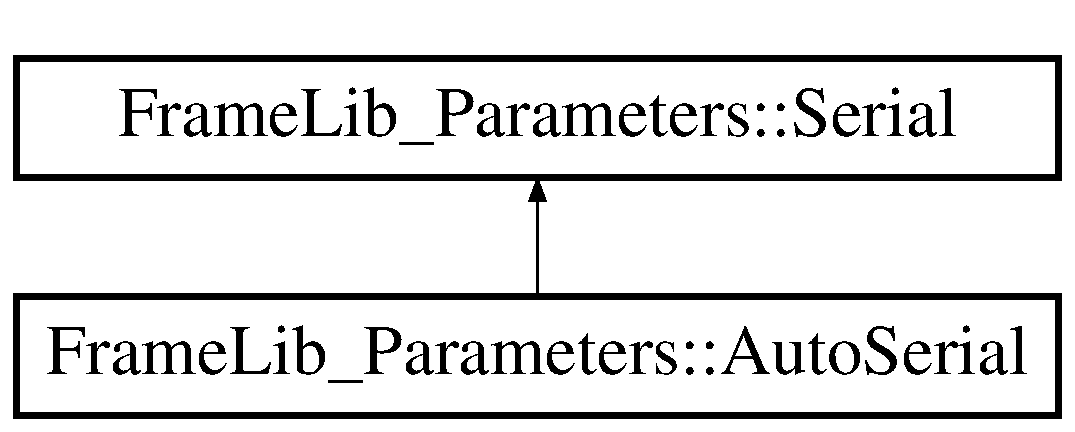
\includegraphics[height=2.000000cm]{class_frame_lib___parameters_1_1_auto_serial}
\end{center}
\end{figure}
\subsection*{Public Member Functions}
\begin{DoxyCompactItemize}
\item 
\hyperlink{class_frame_lib___parameters_1_1_auto_serial_a633ec0dfc1b5a1bdf67b0932e2c132d4}{Auto\+Serial} ()
\item 
\hyperlink{class_frame_lib___parameters_1_1_auto_serial_ade5aeae38060ad0e691517d3d6bc3600}{Auto\+Serial} (size\+\_\+t \hyperlink{class_frame_lib___parameters_1_1_serial_a04ad46904d9fd8119283eae663901886}{size})
\item 
\hyperlink{class_frame_lib___parameters_1_1_auto_serial_a43c7102d42538b237cbacc3e50c655bf}{Auto\+Serial} (const \hyperlink{class_frame_lib___parameters_1_1_serial}{Serial} \&serial)
\item 
\hyperlink{class_frame_lib___parameters_1_1_auto_serial_a9176c245f71bf8f551870863c23fcd28}{Auto\+Serial} (const char $\ast$tag, const char $\ast$string)
\item 
\hyperlink{class_frame_lib___parameters_1_1_auto_serial_adba1790ca1e0ec5376e36dc38469e057}{Auto\+Serial} (const char $\ast$tag, const double $\ast$values, size\+\_\+t N)
\item 
\hyperlink{class_frame_lib___parameters_1_1_auto_serial_a8332e640a34eca6f4c39dc0bd135fdab}{$\sim$\+Auto\+Serial} ()
\item 
void \hyperlink{class_frame_lib___parameters_1_1_auto_serial_a757e1173895b3dc558a7b1a1c0caaae6}{write} (const \hyperlink{class_frame_lib___parameters_1_1_serial}{Serial} $\ast$serialised)
\item 
void \hyperlink{class_frame_lib___parameters_1_1_auto_serial_ae718f5ffe4041355f80bbd0bb25a8205}{write} (const char $\ast$tag, const char $\ast$str)
\item 
void \hyperlink{class_frame_lib___parameters_1_1_auto_serial_aabe8357d608f708e334dcc7fd22ebddd}{write} (const char $\ast$tag, const double $\ast$values, size\+\_\+t N)
\end{DoxyCompactItemize}
\subsection*{Additional Inherited Members}


\subsection{Detailed Description}
an extension of \hyperlink{class_frame_lib___parameters_1_1_serial}{Serial} that manages its own resizable memory. 

\subsection{Constructor \& Destructor Documentation}
\mbox{\Hypertarget{class_frame_lib___parameters_1_1_auto_serial_a633ec0dfc1b5a1bdf67b0932e2c132d4}\label{class_frame_lib___parameters_1_1_auto_serial_a633ec0dfc1b5a1bdf67b0932e2c132d4}} 
\index{Frame\+Lib\+\_\+\+Parameters\+::\+Auto\+Serial@{Frame\+Lib\+\_\+\+Parameters\+::\+Auto\+Serial}!Auto\+Serial@{Auto\+Serial}}
\index{Auto\+Serial@{Auto\+Serial}!Frame\+Lib\+\_\+\+Parameters\+::\+Auto\+Serial@{Frame\+Lib\+\_\+\+Parameters\+::\+Auto\+Serial}}
\subsubsection{\texorpdfstring{Auto\+Serial()}{AutoSerial()}\hspace{0.1cm}{\footnotesize\ttfamily [1/5]}}
{\footnotesize\ttfamily Frame\+Lib\+\_\+\+Parameters\+::\+Auto\+Serial\+::\+Auto\+Serial (\begin{DoxyParamCaption}{ }\end{DoxyParamCaption})\hspace{0.3cm}{\ttfamily [inline]}}

\mbox{\Hypertarget{class_frame_lib___parameters_1_1_auto_serial_ade5aeae38060ad0e691517d3d6bc3600}\label{class_frame_lib___parameters_1_1_auto_serial_ade5aeae38060ad0e691517d3d6bc3600}} 
\index{Frame\+Lib\+\_\+\+Parameters\+::\+Auto\+Serial@{Frame\+Lib\+\_\+\+Parameters\+::\+Auto\+Serial}!Auto\+Serial@{Auto\+Serial}}
\index{Auto\+Serial@{Auto\+Serial}!Frame\+Lib\+\_\+\+Parameters\+::\+Auto\+Serial@{Frame\+Lib\+\_\+\+Parameters\+::\+Auto\+Serial}}
\subsubsection{\texorpdfstring{Auto\+Serial()}{AutoSerial()}\hspace{0.1cm}{\footnotesize\ttfamily [2/5]}}
{\footnotesize\ttfamily Frame\+Lib\+\_\+\+Parameters\+::\+Auto\+Serial\+::\+Auto\+Serial (\begin{DoxyParamCaption}\item[{size\+\_\+t}]{size }\end{DoxyParamCaption})\hspace{0.3cm}{\ttfamily [inline]}}

\mbox{\Hypertarget{class_frame_lib___parameters_1_1_auto_serial_a43c7102d42538b237cbacc3e50c655bf}\label{class_frame_lib___parameters_1_1_auto_serial_a43c7102d42538b237cbacc3e50c655bf}} 
\index{Frame\+Lib\+\_\+\+Parameters\+::\+Auto\+Serial@{Frame\+Lib\+\_\+\+Parameters\+::\+Auto\+Serial}!Auto\+Serial@{Auto\+Serial}}
\index{Auto\+Serial@{Auto\+Serial}!Frame\+Lib\+\_\+\+Parameters\+::\+Auto\+Serial@{Frame\+Lib\+\_\+\+Parameters\+::\+Auto\+Serial}}
\subsubsection{\texorpdfstring{Auto\+Serial()}{AutoSerial()}\hspace{0.1cm}{\footnotesize\ttfamily [3/5]}}
{\footnotesize\ttfamily Frame\+Lib\+\_\+\+Parameters\+::\+Auto\+Serial\+::\+Auto\+Serial (\begin{DoxyParamCaption}\item[{const \hyperlink{class_frame_lib___parameters_1_1_serial}{Serial} \&}]{serial }\end{DoxyParamCaption})\hspace{0.3cm}{\ttfamily [inline]}}

\mbox{\Hypertarget{class_frame_lib___parameters_1_1_auto_serial_a9176c245f71bf8f551870863c23fcd28}\label{class_frame_lib___parameters_1_1_auto_serial_a9176c245f71bf8f551870863c23fcd28}} 
\index{Frame\+Lib\+\_\+\+Parameters\+::\+Auto\+Serial@{Frame\+Lib\+\_\+\+Parameters\+::\+Auto\+Serial}!Auto\+Serial@{Auto\+Serial}}
\index{Auto\+Serial@{Auto\+Serial}!Frame\+Lib\+\_\+\+Parameters\+::\+Auto\+Serial@{Frame\+Lib\+\_\+\+Parameters\+::\+Auto\+Serial}}
\subsubsection{\texorpdfstring{Auto\+Serial()}{AutoSerial()}\hspace{0.1cm}{\footnotesize\ttfamily [4/5]}}
{\footnotesize\ttfamily Frame\+Lib\+\_\+\+Parameters\+::\+Auto\+Serial\+::\+Auto\+Serial (\begin{DoxyParamCaption}\item[{const char $\ast$}]{tag,  }\item[{const char $\ast$}]{string }\end{DoxyParamCaption})\hspace{0.3cm}{\ttfamily [inline]}}

\mbox{\Hypertarget{class_frame_lib___parameters_1_1_auto_serial_adba1790ca1e0ec5376e36dc38469e057}\label{class_frame_lib___parameters_1_1_auto_serial_adba1790ca1e0ec5376e36dc38469e057}} 
\index{Frame\+Lib\+\_\+\+Parameters\+::\+Auto\+Serial@{Frame\+Lib\+\_\+\+Parameters\+::\+Auto\+Serial}!Auto\+Serial@{Auto\+Serial}}
\index{Auto\+Serial@{Auto\+Serial}!Frame\+Lib\+\_\+\+Parameters\+::\+Auto\+Serial@{Frame\+Lib\+\_\+\+Parameters\+::\+Auto\+Serial}}
\subsubsection{\texorpdfstring{Auto\+Serial()}{AutoSerial()}\hspace{0.1cm}{\footnotesize\ttfamily [5/5]}}
{\footnotesize\ttfamily Frame\+Lib\+\_\+\+Parameters\+::\+Auto\+Serial\+::\+Auto\+Serial (\begin{DoxyParamCaption}\item[{const char $\ast$}]{tag,  }\item[{const double $\ast$}]{values,  }\item[{size\+\_\+t}]{N }\end{DoxyParamCaption})\hspace{0.3cm}{\ttfamily [inline]}}

\mbox{\Hypertarget{class_frame_lib___parameters_1_1_auto_serial_a8332e640a34eca6f4c39dc0bd135fdab}\label{class_frame_lib___parameters_1_1_auto_serial_a8332e640a34eca6f4c39dc0bd135fdab}} 
\index{Frame\+Lib\+\_\+\+Parameters\+::\+Auto\+Serial@{Frame\+Lib\+\_\+\+Parameters\+::\+Auto\+Serial}!````~Auto\+Serial@{$\sim$\+Auto\+Serial}}
\index{````~Auto\+Serial@{$\sim$\+Auto\+Serial}!Frame\+Lib\+\_\+\+Parameters\+::\+Auto\+Serial@{Frame\+Lib\+\_\+\+Parameters\+::\+Auto\+Serial}}
\subsubsection{\texorpdfstring{$\sim$\+Auto\+Serial()}{~AutoSerial()}}
{\footnotesize\ttfamily Frame\+Lib\+\_\+\+Parameters\+::\+Auto\+Serial\+::$\sim$\+Auto\+Serial (\begin{DoxyParamCaption}{ }\end{DoxyParamCaption})\hspace{0.3cm}{\ttfamily [inline]}}



\subsection{Member Function Documentation}
\mbox{\Hypertarget{class_frame_lib___parameters_1_1_auto_serial_a757e1173895b3dc558a7b1a1c0caaae6}\label{class_frame_lib___parameters_1_1_auto_serial_a757e1173895b3dc558a7b1a1c0caaae6}} 
\index{Frame\+Lib\+\_\+\+Parameters\+::\+Auto\+Serial@{Frame\+Lib\+\_\+\+Parameters\+::\+Auto\+Serial}!write@{write}}
\index{write@{write}!Frame\+Lib\+\_\+\+Parameters\+::\+Auto\+Serial@{Frame\+Lib\+\_\+\+Parameters\+::\+Auto\+Serial}}
\subsubsection{\texorpdfstring{write()}{write()}\hspace{0.1cm}{\footnotesize\ttfamily [1/3]}}
{\footnotesize\ttfamily void Frame\+Lib\+\_\+\+Parameters\+::\+Auto\+Serial\+::write (\begin{DoxyParamCaption}\item[{const \hyperlink{class_frame_lib___parameters_1_1_serial}{Serial} $\ast$}]{serialised }\end{DoxyParamCaption})\hspace{0.3cm}{\ttfamily [inline]}}

\mbox{\Hypertarget{class_frame_lib___parameters_1_1_auto_serial_ae718f5ffe4041355f80bbd0bb25a8205}\label{class_frame_lib___parameters_1_1_auto_serial_ae718f5ffe4041355f80bbd0bb25a8205}} 
\index{Frame\+Lib\+\_\+\+Parameters\+::\+Auto\+Serial@{Frame\+Lib\+\_\+\+Parameters\+::\+Auto\+Serial}!write@{write}}
\index{write@{write}!Frame\+Lib\+\_\+\+Parameters\+::\+Auto\+Serial@{Frame\+Lib\+\_\+\+Parameters\+::\+Auto\+Serial}}
\subsubsection{\texorpdfstring{write()}{write()}\hspace{0.1cm}{\footnotesize\ttfamily [2/3]}}
{\footnotesize\ttfamily void Frame\+Lib\+\_\+\+Parameters\+::\+Auto\+Serial\+::write (\begin{DoxyParamCaption}\item[{const char $\ast$}]{tag,  }\item[{const char $\ast$}]{str }\end{DoxyParamCaption})\hspace{0.3cm}{\ttfamily [inline]}}

\mbox{\Hypertarget{class_frame_lib___parameters_1_1_auto_serial_aabe8357d608f708e334dcc7fd22ebddd}\label{class_frame_lib___parameters_1_1_auto_serial_aabe8357d608f708e334dcc7fd22ebddd}} 
\index{Frame\+Lib\+\_\+\+Parameters\+::\+Auto\+Serial@{Frame\+Lib\+\_\+\+Parameters\+::\+Auto\+Serial}!write@{write}}
\index{write@{write}!Frame\+Lib\+\_\+\+Parameters\+::\+Auto\+Serial@{Frame\+Lib\+\_\+\+Parameters\+::\+Auto\+Serial}}
\subsubsection{\texorpdfstring{write()}{write()}\hspace{0.1cm}{\footnotesize\ttfamily [3/3]}}
{\footnotesize\ttfamily void Frame\+Lib\+\_\+\+Parameters\+::\+Auto\+Serial\+::write (\begin{DoxyParamCaption}\item[{const char $\ast$}]{tag,  }\item[{const double $\ast$}]{values,  }\item[{size\+\_\+t}]{N }\end{DoxyParamCaption})\hspace{0.3cm}{\ttfamily [inline]}}



The documentation for this class was generated from the following files\+:\begin{DoxyCompactItemize}
\item 
/\+Users/alexharker/\+Documents/\+Max Externals/\+Frame\+Lib/\+Frame\+Lib\+\_\+\+Framework/\hyperlink{_frame_lib___parameters_8h}{Frame\+Lib\+\_\+\+Parameters.\+h}\item 
/\+Users/alexharker/\+Documents/\+Max Externals/\+Frame\+Lib/\+Frame\+Lib\+\_\+\+Framework/\hyperlink{_frame_lib___parameters_8cpp}{Frame\+Lib\+\_\+\+Parameters.\+cpp}\end{DoxyCompactItemize}

\hypertarget{class_delegate_thread}{}\section{Delegate\+Thread Class Reference}
\label{class_delegate_thread}\index{Delegate\+Thread@{Delegate\+Thread}}


{\ttfamily \#include $<$Frame\+Lib\+\_\+\+Threading.\+h$>$}

\subsection*{Public Member Functions}
\begin{DoxyCompactItemize}
\item 
\hyperlink{class_delegate_thread_a96315fa93f55d173f193b1ccc593c0f8}{Delegate\+Thread} (\hyperlink{class_thread_a42f854dd02a3640e422b2f3288067744}{Thread\+::\+Priority\+Level} priority)
\item 
virtual \hyperlink{class_delegate_thread_a19c74ae776c205e9f0ea77119d11cb20}{$\sim$\+Delegate\+Thread} ()
\item 
void \hyperlink{class_delegate_thread_a45a890ecb21c6e560ff9e391837453ad}{start} ()
\item 
void \hyperlink{class_delegate_thread_a487fadd304c533222b14ff950bc05744}{join} ()
\item 
bool \hyperlink{class_delegate_thread_a2024b79dc8f91a1a5af085f41059bf1e}{signal} ()
\item 
bool \hyperlink{class_delegate_thread_a0f03ed4723a9517afb896108d20927e8}{completed} ()
\end{DoxyCompactItemize}


\subsection{Constructor \& Destructor Documentation}
\mbox{\Hypertarget{class_delegate_thread_a96315fa93f55d173f193b1ccc593c0f8}\label{class_delegate_thread_a96315fa93f55d173f193b1ccc593c0f8}} 
\index{Delegate\+Thread@{Delegate\+Thread}!Delegate\+Thread@{Delegate\+Thread}}
\index{Delegate\+Thread@{Delegate\+Thread}!Delegate\+Thread@{Delegate\+Thread}}
\subsubsection{\texorpdfstring{Delegate\+Thread()}{DelegateThread()}}
{\footnotesize\ttfamily Delegate\+Thread\+::\+Delegate\+Thread (\begin{DoxyParamCaption}\item[{\hyperlink{class_thread_a42f854dd02a3640e422b2f3288067744}{Thread\+::\+Priority\+Level}}]{priority }\end{DoxyParamCaption})\hspace{0.3cm}{\ttfamily [inline]}}

\mbox{\Hypertarget{class_delegate_thread_a19c74ae776c205e9f0ea77119d11cb20}\label{class_delegate_thread_a19c74ae776c205e9f0ea77119d11cb20}} 
\index{Delegate\+Thread@{Delegate\+Thread}!````~Delegate\+Thread@{$\sim$\+Delegate\+Thread}}
\index{````~Delegate\+Thread@{$\sim$\+Delegate\+Thread}!Delegate\+Thread@{Delegate\+Thread}}
\subsubsection{\texorpdfstring{$\sim$\+Delegate\+Thread()}{~DelegateThread()}}
{\footnotesize\ttfamily virtual Delegate\+Thread\+::$\sim$\+Delegate\+Thread (\begin{DoxyParamCaption}{ }\end{DoxyParamCaption})\hspace{0.3cm}{\ttfamily [inline]}, {\ttfamily [virtual]}}



\subsection{Member Function Documentation}
\mbox{\Hypertarget{class_delegate_thread_a0f03ed4723a9517afb896108d20927e8}\label{class_delegate_thread_a0f03ed4723a9517afb896108d20927e8}} 
\index{Delegate\+Thread@{Delegate\+Thread}!completed@{completed}}
\index{completed@{completed}!Delegate\+Thread@{Delegate\+Thread}}
\subsubsection{\texorpdfstring{completed()}{completed()}}
{\footnotesize\ttfamily bool Delegate\+Thread\+::completed (\begin{DoxyParamCaption}{ }\end{DoxyParamCaption})}

\mbox{\Hypertarget{class_delegate_thread_a487fadd304c533222b14ff950bc05744}\label{class_delegate_thread_a487fadd304c533222b14ff950bc05744}} 
\index{Delegate\+Thread@{Delegate\+Thread}!join@{join}}
\index{join@{join}!Delegate\+Thread@{Delegate\+Thread}}
\subsubsection{\texorpdfstring{join()}{join()}}
{\footnotesize\ttfamily void Delegate\+Thread\+::join (\begin{DoxyParamCaption}{ }\end{DoxyParamCaption})}

\mbox{\Hypertarget{class_delegate_thread_a2024b79dc8f91a1a5af085f41059bf1e}\label{class_delegate_thread_a2024b79dc8f91a1a5af085f41059bf1e}} 
\index{Delegate\+Thread@{Delegate\+Thread}!signal@{signal}}
\index{signal@{signal}!Delegate\+Thread@{Delegate\+Thread}}
\subsubsection{\texorpdfstring{signal()}{signal()}}
{\footnotesize\ttfamily bool Delegate\+Thread\+::signal (\begin{DoxyParamCaption}{ }\end{DoxyParamCaption})}

\mbox{\Hypertarget{class_delegate_thread_a45a890ecb21c6e560ff9e391837453ad}\label{class_delegate_thread_a45a890ecb21c6e560ff9e391837453ad}} 
\index{Delegate\+Thread@{Delegate\+Thread}!start@{start}}
\index{start@{start}!Delegate\+Thread@{Delegate\+Thread}}
\subsubsection{\texorpdfstring{start()}{start()}}
{\footnotesize\ttfamily void Delegate\+Thread\+::start (\begin{DoxyParamCaption}{ }\end{DoxyParamCaption})\hspace{0.3cm}{\ttfamily [inline]}}



The documentation for this class was generated from the following files\+:\begin{DoxyCompactItemize}
\item 
/\+Users/alexharker/\+Documents/\+Max Externals/\+Frame\+Lib/\+Frame\+Lib\+\_\+\+Framework/\hyperlink{_frame_lib___threading_8h}{Frame\+Lib\+\_\+\+Threading.\+h}\item 
/\+Users/alexharker/\+Documents/\+Max Externals/\+Frame\+Lib/\+Frame\+Lib\+\_\+\+Framework/\hyperlink{_frame_lib___threading_8cpp}{Frame\+Lib\+\_\+\+Threading.\+cpp}\end{DoxyCompactItemize}

\hypertarget{class_f_l___f_p}{}\section{F\+L\+\_\+\+FP Class Reference}
\label{class_f_l___f_p}\index{F\+L\+\_\+\+FP@{F\+L\+\_\+\+FP}}


high-\/precision unsigned fixed-\/point numerical format.  




{\ttfamily \#include $<$Frame\+Lib\+\_\+\+Fixed\+Point.\+h$>$}

Inheritance diagram for F\+L\+\_\+\+FP\+:\begin{figure}[H]
\begin{center}
\leavevmode
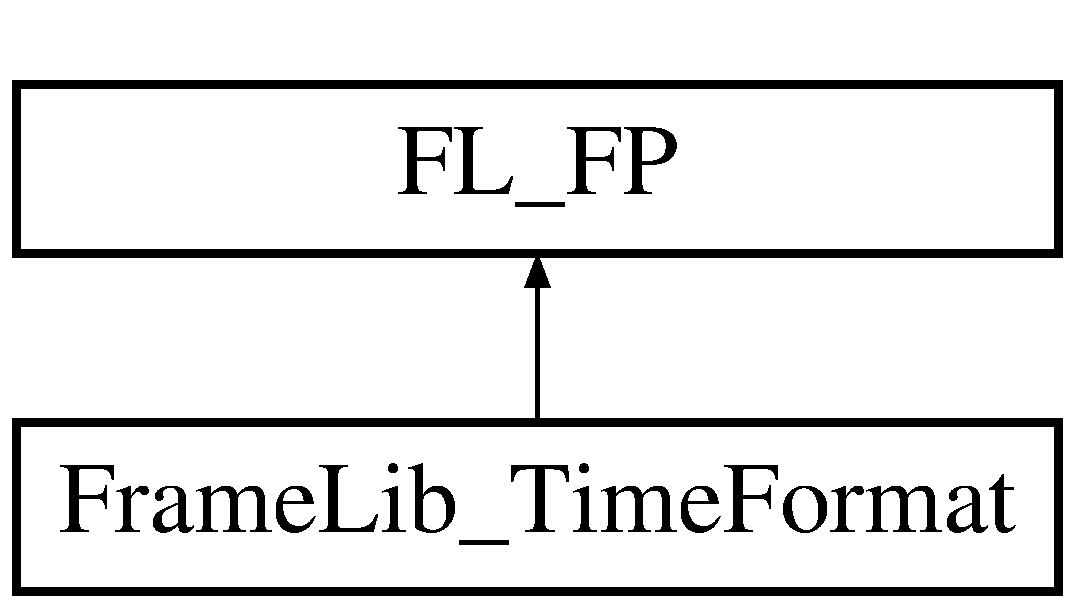
\includegraphics[height=2.000000cm]{class_f_l___f_p}
\end{center}
\end{figure}
\subsection*{Public Member Functions}
\begin{DoxyCompactItemize}
\item 
\hyperlink{class_f_l___f_p_a2db44ca3f010e72af1a0ba97f443fe93}{F\+L\+\_\+\+FP} ()
\item 
\hyperlink{class_f_l___f_p_ac233226f5a38c1180b00965cda0b2ba1}{F\+L\+\_\+\+FP} (uint64\+\_\+t a, uint64\+\_\+t b)
\item 
\hyperlink{class_f_l___f_p_ae69dbbbcee3563f7ff4e3102dd137c05}{F\+L\+\_\+\+FP} (const \hyperlink{struct_f_l___s_p}{F\+L\+\_\+\+SP} \&val)
\item 
\hyperlink{class_f_l___f_p_a552b545bb667d5a6436e89f33586e9fa}{F\+L\+\_\+\+FP} (const double \&val)
\item 
uint64\+\_\+t \hyperlink{class_f_l___f_p_acffd4f751e5042dbed4a28bfe3f90ea5}{int\+Val} () const
\item 
uint64\+\_\+t \hyperlink{class_f_l___f_p_adeac9cc0d327d4759ac35890c13978c0}{frac\+Val} () const
\item 
\hyperlink{class_f_l___f_p}{F\+L\+\_\+\+FP} \& \hyperlink{class_f_l___f_p_ab07d8c341752a6668a3a8a6e0d8ba2c7}{operator+=} (const \hyperlink{class_f_l___f_p}{F\+L\+\_\+\+FP} \&b)
\item 
\hyperlink{class_f_l___f_p}{F\+L\+\_\+\+FP} \& \hyperlink{class_f_l___f_p_a494e954f36fbfd791dfc2117e0de4baa}{operator-\/=} (const \hyperlink{class_f_l___f_p}{F\+L\+\_\+\+FP} \&b)
\item 
\hyperlink{class_f_l___f_p}{F\+L\+\_\+\+FP} \& \hyperlink{class_f_l___f_p_a04123cec30a145c37cfdaa2030ecba5e}{operator$\ast$=} (const \hyperlink{class_f_l___f_p}{F\+L\+\_\+\+FP} \&b)
\item 
\hyperlink{class_f_l___f_p}{F\+L\+\_\+\+FP} \& \hyperlink{class_f_l___f_p_a2bbae2b6138642ae4cf90eb7b3a1ea5f}{operator/=} (const \hyperlink{class_f_l___f_p}{F\+L\+\_\+\+FP} \&b)
\item 
\hyperlink{class_f_l___f_p}{F\+L\+\_\+\+FP} \& \hyperlink{class_f_l___f_p_a883f8d6a0d34a3af9a35654b25f0ba7c}{operator++} ()
\item 
\hyperlink{class_f_l___f_p}{F\+L\+\_\+\+FP} \hyperlink{class_f_l___f_p_a2feeebae2b863b1955232473b4f62db0}{operator++} (int)
\item 
\hyperlink{class_f_l___f_p}{F\+L\+\_\+\+FP} \& \hyperlink{class_f_l___f_p_a3e9f6cc369b21fe2d188ebeca60a3df4}{operator-\/-\/} ()
\item 
\hyperlink{class_f_l___f_p}{F\+L\+\_\+\+FP} \& \hyperlink{class_f_l___f_p_a1a15cf670b1b9a8e66d6ba910bcb8e62}{operator-\/-\/} (int)
\item 
\hyperlink{class_f_l___f_p_af0526310d4b3754485f712b5dfb96b32}{operator double} () const
\item 
\hyperlink{class_f_l___f_p}{F\+L\+\_\+\+FP} \& \hyperlink{class_f_l___f_p_a676730a35c5b8e87c672336a34fa684d}{operator=} (const double \&a)
\item 
\hyperlink{class_f_l___f_p}{F\+L\+\_\+\+FP} \& \hyperlink{class_f_l___f_p_a858ea714be8344937bf2a1b78ff64b55}{operator+=} (const double \&b)
\item 
\hyperlink{class_f_l___f_p}{F\+L\+\_\+\+FP} \& \hyperlink{class_f_l___f_p_a43876e6b2d9ce28d6c230e75dfbe8cd5}{operator-\/=} (const double \&b)
\item 
\hyperlink{class_f_l___f_p}{F\+L\+\_\+\+FP} \& \hyperlink{class_f_l___f_p_aa5786b1ca47a70a1c61c0da74bfc5036}{operator$\ast$=} (const double \&b)
\item 
\hyperlink{class_f_l___f_p}{F\+L\+\_\+\+FP} \& \hyperlink{class_f_l___f_p_ab49fcbb06bdc25f29cc238f4c21c722d}{operator/=} (const double \&b)
\end{DoxyCompactItemize}
\subsection*{Friends}
\begin{DoxyCompactItemize}
\item 
bool \hyperlink{class_f_l___f_p_a7f68a65590040b22d55e29f700a70090}{operator==} (const \hyperlink{class_f_l___f_p}{F\+L\+\_\+\+FP} \&a, const \hyperlink{class_f_l___f_p}{F\+L\+\_\+\+FP} \&b)
\item 
bool \hyperlink{class_f_l___f_p_a694ee4bd94433b815c7f4e5f7a2acd50}{operator!=} (const \hyperlink{class_f_l___f_p}{F\+L\+\_\+\+FP} \&a, const \hyperlink{class_f_l___f_p}{F\+L\+\_\+\+FP} \&b)
\item 
bool \hyperlink{class_f_l___f_p_a7a645d400e5b6aeaf8a3ea2a4512ab9e}{operator$<$} (const \hyperlink{class_f_l___f_p}{F\+L\+\_\+\+FP} \&a, const \hyperlink{class_f_l___f_p}{F\+L\+\_\+\+FP} \&b)
\item 
bool \hyperlink{class_f_l___f_p_ab237b013e66f2d39a3bb466e36741baf}{operator$>$} (const \hyperlink{class_f_l___f_p}{F\+L\+\_\+\+FP} \&a, const \hyperlink{class_f_l___f_p}{F\+L\+\_\+\+FP} \&b)
\item 
bool \hyperlink{class_f_l___f_p_a420177af32f27b84621b1bdc1db5d29a}{operator$<$=} (const \hyperlink{class_f_l___f_p}{F\+L\+\_\+\+FP} \&a, const \hyperlink{class_f_l___f_p}{F\+L\+\_\+\+FP} \&b)
\item 
bool \hyperlink{class_f_l___f_p_a496bb5bc687d589a5ec23c0b81dc5fb2}{operator$>$=} (const \hyperlink{class_f_l___f_p}{F\+L\+\_\+\+FP} \&a, const \hyperlink{class_f_l___f_p}{F\+L\+\_\+\+FP} \&b)
\item 
bool \hyperlink{class_f_l___f_p_a14d7541c865b9e57eaaca1c3fd2c6240}{operator!} (const \hyperlink{class_f_l___f_p}{F\+L\+\_\+\+FP} \&b)
\item 
\hyperlink{class_f_l___f_p}{F\+L\+\_\+\+FP} \hyperlink{class_f_l___f_p_a96dfe1fef405deebcdd77739a80baf4e}{operator+} (const \hyperlink{class_f_l___f_p}{F\+L\+\_\+\+FP} \&a, const \hyperlink{class_f_l___f_p}{F\+L\+\_\+\+FP} \&b)
\item 
\hyperlink{class_f_l___f_p}{F\+L\+\_\+\+FP} \hyperlink{class_f_l___f_p_a29c8d46e78c5c3a20fdfbf9904f0a25d}{operator-\/} (const \hyperlink{class_f_l___f_p}{F\+L\+\_\+\+FP} \&a, const \hyperlink{class_f_l___f_p}{F\+L\+\_\+\+FP} \&b)
\item 
\hyperlink{class_f_l___f_p}{F\+L\+\_\+\+FP} \hyperlink{class_f_l___f_p_a7c9e13210a3e8f9ef270a4895b1fc0d3}{operator$\ast$} (const \hyperlink{class_f_l___f_p}{F\+L\+\_\+\+FP} \&a, const \hyperlink{class_f_l___f_p}{F\+L\+\_\+\+FP} \&b)
\item 
\hyperlink{class_f_l___f_p}{F\+L\+\_\+\+FP} \hyperlink{class_f_l___f_p_a746b7c97a3194b33df5e6e04ce0ce5e8}{operator/} (const \hyperlink{class_f_l___f_p}{F\+L\+\_\+\+FP} \&a, const \hyperlink{class_f_l___f_p}{F\+L\+\_\+\+FP} \&b)
\item 
bool \hyperlink{class_f_l___f_p_a666442f1b900ba2e6680d77ec4261a9e}{operator==} (const \hyperlink{class_f_l___f_p}{F\+L\+\_\+\+FP} \&a, const double \&b)
\item 
bool \hyperlink{class_f_l___f_p_a8b8fd18407f83f9bbf63012179eb694d}{operator==} (const double \&a, const \hyperlink{class_f_l___f_p}{F\+L\+\_\+\+FP} \&b)
\item 
bool \hyperlink{class_f_l___f_p_a3c240fef687da52fed8f3646a924d91e}{operator!=} (const \hyperlink{class_f_l___f_p}{F\+L\+\_\+\+FP} \&a, const double \&b)
\item 
bool \hyperlink{class_f_l___f_p_a699d74159c9061491364140ac24a568b}{operator!=} (const double \&a, const \hyperlink{class_f_l___f_p}{F\+L\+\_\+\+FP} \&b)
\item 
bool \hyperlink{class_f_l___f_p_ae0d89fcb254db9759b80cca31de5ee00}{operator$<$} (const \hyperlink{class_f_l___f_p}{F\+L\+\_\+\+FP} \&a, const double \&b)
\item 
bool \hyperlink{class_f_l___f_p_af1a4354ad8a5d501c5d9f3a784ca3b95}{operator$<$} (const double \&a, const \hyperlink{class_f_l___f_p}{F\+L\+\_\+\+FP} \&b)
\item 
bool \hyperlink{class_f_l___f_p_acc2241533b3b7f53f6e8bc40c77233a5}{operator$>$} (const \hyperlink{class_f_l___f_p}{F\+L\+\_\+\+FP} \&a, const double \&b)
\item 
bool \hyperlink{class_f_l___f_p_aed84a1784274a020d95f2c01746f2b5c}{operator$>$} (const double \&a, const \hyperlink{class_f_l___f_p}{F\+L\+\_\+\+FP} \&b)
\item 
bool \hyperlink{class_f_l___f_p_a2453dc97f7fd85f4a1c07f5d888c4b87}{operator$<$=} (const \hyperlink{class_f_l___f_p}{F\+L\+\_\+\+FP} \&a, const double \&b)
\item 
bool \hyperlink{class_f_l___f_p_a78d1e2f69d82635ea82a2b717d79d5bb}{operator$<$=} (const double \&a, const \hyperlink{class_f_l___f_p}{F\+L\+\_\+\+FP} \&b)
\item 
bool \hyperlink{class_f_l___f_p_ace9ff2ae86cfecb59b601ef983b5189d}{operator$>$=} (const \hyperlink{class_f_l___f_p}{F\+L\+\_\+\+FP} \&a, const double \&b)
\item 
bool \hyperlink{class_f_l___f_p_a1f7bf9f00e36c130033949619f5261dd}{operator$>$=} (const double \&a, const \hyperlink{class_f_l___f_p}{F\+L\+\_\+\+FP} \&b)
\item 
\hyperlink{class_f_l___f_p}{F\+L\+\_\+\+FP} \hyperlink{class_f_l___f_p_a230919bb5d28822bd782aa7ca3465eba}{operator+} (const \hyperlink{class_f_l___f_p}{F\+L\+\_\+\+FP} \&a, const double \&b)
\item 
\hyperlink{class_f_l___f_p}{F\+L\+\_\+\+FP} \hyperlink{class_f_l___f_p_a4934b87fe91ceefeb77cc0fbf926329c}{operator+} (const double \&a, const \hyperlink{class_f_l___f_p}{F\+L\+\_\+\+FP} \&b)
\item 
\hyperlink{class_f_l___f_p}{F\+L\+\_\+\+FP} \hyperlink{class_f_l___f_p_a4355725c40ad917191e6384f58177915}{operator-\/} (const \hyperlink{class_f_l___f_p}{F\+L\+\_\+\+FP} \&a, const double \&b)
\item 
\hyperlink{class_f_l___f_p}{F\+L\+\_\+\+FP} \hyperlink{class_f_l___f_p_afede6b6bcb4b0e35903a5e47cb0096e1}{operator-\/} (const double \&a, const \hyperlink{class_f_l___f_p}{F\+L\+\_\+\+FP} \&b)
\item 
\hyperlink{class_f_l___f_p}{F\+L\+\_\+\+FP} \hyperlink{class_f_l___f_p_a4d88f005bc60cbdceb070335a94a068a}{operator$\ast$} (const \hyperlink{class_f_l___f_p}{F\+L\+\_\+\+FP} \&a, const double \&b)
\item 
\hyperlink{class_f_l___f_p}{F\+L\+\_\+\+FP} \hyperlink{class_f_l___f_p_a248f294ecf7ddc53650ef72b848e6bb5}{operator$\ast$} (const double \&a, const \hyperlink{class_f_l___f_p}{F\+L\+\_\+\+FP} \&b)
\item 
\hyperlink{class_f_l___f_p}{F\+L\+\_\+\+FP} \hyperlink{class_f_l___f_p_a10e4527f31f6a72dfc92215a83bbf439}{operator/} (const \hyperlink{class_f_l___f_p}{F\+L\+\_\+\+FP} \&a, const double \&b)
\item 
\hyperlink{class_f_l___f_p}{F\+L\+\_\+\+FP} \hyperlink{class_f_l___f_p_a748c3789021613fe839afe4289689f88}{operator/} (const double \&a, const \hyperlink{class_f_l___f_p}{F\+L\+\_\+\+FP} \&b)
\end{DoxyCompactItemize}


\subsection{Detailed Description}
high-\/precision unsigned fixed-\/point numerical format. 

This unsigned type allows for 64 bits of integer precision and 64 bits of fractional precision. Basic arithmetic and comparison operators are supported, for this type, and when used in conjunction with double-\/precision floating-\/point numbers. The primary purpose of this type is to precisely represent the time in samples in Frame\+Lib. 

\subsection{Constructor \& Destructor Documentation}
\mbox{\Hypertarget{class_f_l___f_p_a2db44ca3f010e72af1a0ba97f443fe93}\label{class_f_l___f_p_a2db44ca3f010e72af1a0ba97f443fe93}} 
\index{F\+L\+\_\+\+FP@{F\+L\+\_\+\+FP}!F\+L\+\_\+\+FP@{F\+L\+\_\+\+FP}}
\index{F\+L\+\_\+\+FP@{F\+L\+\_\+\+FP}!F\+L\+\_\+\+FP@{F\+L\+\_\+\+FP}}
\subsubsection{\texorpdfstring{F\+L\+\_\+\+F\+P()}{FL\_FP()}\hspace{0.1cm}{\footnotesize\ttfamily [1/4]}}
{\footnotesize\ttfamily F\+L\+\_\+\+F\+P\+::\+F\+L\+\_\+\+FP (\begin{DoxyParamCaption}{ }\end{DoxyParamCaption})\hspace{0.3cm}{\ttfamily [inline]}}

\mbox{\Hypertarget{class_f_l___f_p_ac233226f5a38c1180b00965cda0b2ba1}\label{class_f_l___f_p_ac233226f5a38c1180b00965cda0b2ba1}} 
\index{F\+L\+\_\+\+FP@{F\+L\+\_\+\+FP}!F\+L\+\_\+\+FP@{F\+L\+\_\+\+FP}}
\index{F\+L\+\_\+\+FP@{F\+L\+\_\+\+FP}!F\+L\+\_\+\+FP@{F\+L\+\_\+\+FP}}
\subsubsection{\texorpdfstring{F\+L\+\_\+\+F\+P()}{FL\_FP()}\hspace{0.1cm}{\footnotesize\ttfamily [2/4]}}
{\footnotesize\ttfamily F\+L\+\_\+\+F\+P\+::\+F\+L\+\_\+\+FP (\begin{DoxyParamCaption}\item[{uint64\+\_\+t}]{a,  }\item[{uint64\+\_\+t}]{b }\end{DoxyParamCaption})\hspace{0.3cm}{\ttfamily [inline]}}

\mbox{\Hypertarget{class_f_l___f_p_ae69dbbbcee3563f7ff4e3102dd137c05}\label{class_f_l___f_p_ae69dbbbcee3563f7ff4e3102dd137c05}} 
\index{F\+L\+\_\+\+FP@{F\+L\+\_\+\+FP}!F\+L\+\_\+\+FP@{F\+L\+\_\+\+FP}}
\index{F\+L\+\_\+\+FP@{F\+L\+\_\+\+FP}!F\+L\+\_\+\+FP@{F\+L\+\_\+\+FP}}
\subsubsection{\texorpdfstring{F\+L\+\_\+\+F\+P()}{FL\_FP()}\hspace{0.1cm}{\footnotesize\ttfamily [3/4]}}
{\footnotesize\ttfamily F\+L\+\_\+\+F\+P\+::\+F\+L\+\_\+\+FP (\begin{DoxyParamCaption}\item[{const \hyperlink{struct_f_l___s_p}{F\+L\+\_\+\+SP} \&}]{val }\end{DoxyParamCaption})}

\mbox{\Hypertarget{class_f_l___f_p_a552b545bb667d5a6436e89f33586e9fa}\label{class_f_l___f_p_a552b545bb667d5a6436e89f33586e9fa}} 
\index{F\+L\+\_\+\+FP@{F\+L\+\_\+\+FP}!F\+L\+\_\+\+FP@{F\+L\+\_\+\+FP}}
\index{F\+L\+\_\+\+FP@{F\+L\+\_\+\+FP}!F\+L\+\_\+\+FP@{F\+L\+\_\+\+FP}}
\subsubsection{\texorpdfstring{F\+L\+\_\+\+F\+P()}{FL\_FP()}\hspace{0.1cm}{\footnotesize\ttfamily [4/4]}}
{\footnotesize\ttfamily F\+L\+\_\+\+F\+P\+::\+F\+L\+\_\+\+FP (\begin{DoxyParamCaption}\item[{const double \&}]{val }\end{DoxyParamCaption})}



\subsection{Member Function Documentation}
\mbox{\Hypertarget{class_f_l___f_p_adeac9cc0d327d4759ac35890c13978c0}\label{class_f_l___f_p_adeac9cc0d327d4759ac35890c13978c0}} 
\index{F\+L\+\_\+\+FP@{F\+L\+\_\+\+FP}!frac\+Val@{frac\+Val}}
\index{frac\+Val@{frac\+Val}!F\+L\+\_\+\+FP@{F\+L\+\_\+\+FP}}
\subsubsection{\texorpdfstring{frac\+Val()}{fracVal()}}
{\footnotesize\ttfamily uint64\+\_\+t F\+L\+\_\+\+F\+P\+::frac\+Val (\begin{DoxyParamCaption}{ }\end{DoxyParamCaption}) const\hspace{0.3cm}{\ttfamily [inline]}}

\mbox{\Hypertarget{class_f_l___f_p_acffd4f751e5042dbed4a28bfe3f90ea5}\label{class_f_l___f_p_acffd4f751e5042dbed4a28bfe3f90ea5}} 
\index{F\+L\+\_\+\+FP@{F\+L\+\_\+\+FP}!int\+Val@{int\+Val}}
\index{int\+Val@{int\+Val}!F\+L\+\_\+\+FP@{F\+L\+\_\+\+FP}}
\subsubsection{\texorpdfstring{int\+Val()}{intVal()}}
{\footnotesize\ttfamily uint64\+\_\+t F\+L\+\_\+\+F\+P\+::int\+Val (\begin{DoxyParamCaption}{ }\end{DoxyParamCaption}) const\hspace{0.3cm}{\ttfamily [inline]}}

\mbox{\Hypertarget{class_f_l___f_p_af0526310d4b3754485f712b5dfb96b32}\label{class_f_l___f_p_af0526310d4b3754485f712b5dfb96b32}} 
\index{F\+L\+\_\+\+FP@{F\+L\+\_\+\+FP}!operator double@{operator double}}
\index{operator double@{operator double}!F\+L\+\_\+\+FP@{F\+L\+\_\+\+FP}}
\subsubsection{\texorpdfstring{operator double()}{operator double()}}
{\footnotesize\ttfamily F\+L\+\_\+\+F\+P\+::operator double (\begin{DoxyParamCaption}{ }\end{DoxyParamCaption}) const\hspace{0.3cm}{\ttfamily [inline]}}

\mbox{\Hypertarget{class_f_l___f_p_a04123cec30a145c37cfdaa2030ecba5e}\label{class_f_l___f_p_a04123cec30a145c37cfdaa2030ecba5e}} 
\index{F\+L\+\_\+\+FP@{F\+L\+\_\+\+FP}!operator$\ast$=@{operator$\ast$=}}
\index{operator$\ast$=@{operator$\ast$=}!F\+L\+\_\+\+FP@{F\+L\+\_\+\+FP}}
\subsubsection{\texorpdfstring{operator$\ast$=()}{operator*=()}\hspace{0.1cm}{\footnotesize\ttfamily [1/2]}}
{\footnotesize\ttfamily \hyperlink{class_f_l___f_p}{F\+L\+\_\+\+FP}\& F\+L\+\_\+\+F\+P\+::operator$\ast$= (\begin{DoxyParamCaption}\item[{const \hyperlink{class_f_l___f_p}{F\+L\+\_\+\+FP} \&}]{b }\end{DoxyParamCaption})\hspace{0.3cm}{\ttfamily [inline]}}

\mbox{\Hypertarget{class_f_l___f_p_aa5786b1ca47a70a1c61c0da74bfc5036}\label{class_f_l___f_p_aa5786b1ca47a70a1c61c0da74bfc5036}} 
\index{F\+L\+\_\+\+FP@{F\+L\+\_\+\+FP}!operator$\ast$=@{operator$\ast$=}}
\index{operator$\ast$=@{operator$\ast$=}!F\+L\+\_\+\+FP@{F\+L\+\_\+\+FP}}
\subsubsection{\texorpdfstring{operator$\ast$=()}{operator*=()}\hspace{0.1cm}{\footnotesize\ttfamily [2/2]}}
{\footnotesize\ttfamily \hyperlink{class_f_l___f_p}{F\+L\+\_\+\+FP}\& F\+L\+\_\+\+F\+P\+::operator$\ast$= (\begin{DoxyParamCaption}\item[{const double \&}]{b }\end{DoxyParamCaption})\hspace{0.3cm}{\ttfamily [inline]}}

\mbox{\Hypertarget{class_f_l___f_p_a883f8d6a0d34a3af9a35654b25f0ba7c}\label{class_f_l___f_p_a883f8d6a0d34a3af9a35654b25f0ba7c}} 
\index{F\+L\+\_\+\+FP@{F\+L\+\_\+\+FP}!operator++@{operator++}}
\index{operator++@{operator++}!F\+L\+\_\+\+FP@{F\+L\+\_\+\+FP}}
\subsubsection{\texorpdfstring{operator++()}{operator++()}\hspace{0.1cm}{\footnotesize\ttfamily [1/2]}}
{\footnotesize\ttfamily \hyperlink{class_f_l___f_p}{F\+L\+\_\+\+FP}\& F\+L\+\_\+\+F\+P\+::operator++ (\begin{DoxyParamCaption}{ }\end{DoxyParamCaption})\hspace{0.3cm}{\ttfamily [inline]}}

\mbox{\Hypertarget{class_f_l___f_p_a2feeebae2b863b1955232473b4f62db0}\label{class_f_l___f_p_a2feeebae2b863b1955232473b4f62db0}} 
\index{F\+L\+\_\+\+FP@{F\+L\+\_\+\+FP}!operator++@{operator++}}
\index{operator++@{operator++}!F\+L\+\_\+\+FP@{F\+L\+\_\+\+FP}}
\subsubsection{\texorpdfstring{operator++()}{operator++()}\hspace{0.1cm}{\footnotesize\ttfamily [2/2]}}
{\footnotesize\ttfamily \hyperlink{class_f_l___f_p}{F\+L\+\_\+\+FP} F\+L\+\_\+\+F\+P\+::operator++ (\begin{DoxyParamCaption}\item[{int}]{ }\end{DoxyParamCaption})\hspace{0.3cm}{\ttfamily [inline]}}

\mbox{\Hypertarget{class_f_l___f_p_ab07d8c341752a6668a3a8a6e0d8ba2c7}\label{class_f_l___f_p_ab07d8c341752a6668a3a8a6e0d8ba2c7}} 
\index{F\+L\+\_\+\+FP@{F\+L\+\_\+\+FP}!operator+=@{operator+=}}
\index{operator+=@{operator+=}!F\+L\+\_\+\+FP@{F\+L\+\_\+\+FP}}
\subsubsection{\texorpdfstring{operator+=()}{operator+=()}\hspace{0.1cm}{\footnotesize\ttfamily [1/2]}}
{\footnotesize\ttfamily \hyperlink{class_f_l___f_p}{F\+L\+\_\+\+FP}\& F\+L\+\_\+\+F\+P\+::operator+= (\begin{DoxyParamCaption}\item[{const \hyperlink{class_f_l___f_p}{F\+L\+\_\+\+FP} \&}]{b }\end{DoxyParamCaption})\hspace{0.3cm}{\ttfamily [inline]}}

\mbox{\Hypertarget{class_f_l___f_p_a858ea714be8344937bf2a1b78ff64b55}\label{class_f_l___f_p_a858ea714be8344937bf2a1b78ff64b55}} 
\index{F\+L\+\_\+\+FP@{F\+L\+\_\+\+FP}!operator+=@{operator+=}}
\index{operator+=@{operator+=}!F\+L\+\_\+\+FP@{F\+L\+\_\+\+FP}}
\subsubsection{\texorpdfstring{operator+=()}{operator+=()}\hspace{0.1cm}{\footnotesize\ttfamily [2/2]}}
{\footnotesize\ttfamily \hyperlink{class_f_l___f_p}{F\+L\+\_\+\+FP}\& F\+L\+\_\+\+F\+P\+::operator+= (\begin{DoxyParamCaption}\item[{const double \&}]{b }\end{DoxyParamCaption})\hspace{0.3cm}{\ttfamily [inline]}}

\mbox{\Hypertarget{class_f_l___f_p_a3e9f6cc369b21fe2d188ebeca60a3df4}\label{class_f_l___f_p_a3e9f6cc369b21fe2d188ebeca60a3df4}} 
\index{F\+L\+\_\+\+FP@{F\+L\+\_\+\+FP}!operator-\/-\/@{operator-\/-\/}}
\index{operator-\/-\/@{operator-\/-\/}!F\+L\+\_\+\+FP@{F\+L\+\_\+\+FP}}
\subsubsection{\texorpdfstring{operator-\/-\/()}{operator--()}\hspace{0.1cm}{\footnotesize\ttfamily [1/2]}}
{\footnotesize\ttfamily \hyperlink{class_f_l___f_p}{F\+L\+\_\+\+FP}\& F\+L\+\_\+\+F\+P\+::operator-\/-\/ (\begin{DoxyParamCaption}{ }\end{DoxyParamCaption})\hspace{0.3cm}{\ttfamily [inline]}}

\mbox{\Hypertarget{class_f_l___f_p_a1a15cf670b1b9a8e66d6ba910bcb8e62}\label{class_f_l___f_p_a1a15cf670b1b9a8e66d6ba910bcb8e62}} 
\index{F\+L\+\_\+\+FP@{F\+L\+\_\+\+FP}!operator-\/-\/@{operator-\/-\/}}
\index{operator-\/-\/@{operator-\/-\/}!F\+L\+\_\+\+FP@{F\+L\+\_\+\+FP}}
\subsubsection{\texorpdfstring{operator-\/-\/()}{operator--()}\hspace{0.1cm}{\footnotesize\ttfamily [2/2]}}
{\footnotesize\ttfamily \hyperlink{class_f_l___f_p}{F\+L\+\_\+\+FP}\& F\+L\+\_\+\+F\+P\+::operator-\/-\/ (\begin{DoxyParamCaption}\item[{int}]{ }\end{DoxyParamCaption})\hspace{0.3cm}{\ttfamily [inline]}}

\mbox{\Hypertarget{class_f_l___f_p_a494e954f36fbfd791dfc2117e0de4baa}\label{class_f_l___f_p_a494e954f36fbfd791dfc2117e0de4baa}} 
\index{F\+L\+\_\+\+FP@{F\+L\+\_\+\+FP}!operator-\/=@{operator-\/=}}
\index{operator-\/=@{operator-\/=}!F\+L\+\_\+\+FP@{F\+L\+\_\+\+FP}}
\subsubsection{\texorpdfstring{operator-\/=()}{operator-=()}\hspace{0.1cm}{\footnotesize\ttfamily [1/2]}}
{\footnotesize\ttfamily \hyperlink{class_f_l___f_p}{F\+L\+\_\+\+FP}\& F\+L\+\_\+\+F\+P\+::operator-\/= (\begin{DoxyParamCaption}\item[{const \hyperlink{class_f_l___f_p}{F\+L\+\_\+\+FP} \&}]{b }\end{DoxyParamCaption})\hspace{0.3cm}{\ttfamily [inline]}}

\mbox{\Hypertarget{class_f_l___f_p_a43876e6b2d9ce28d6c230e75dfbe8cd5}\label{class_f_l___f_p_a43876e6b2d9ce28d6c230e75dfbe8cd5}} 
\index{F\+L\+\_\+\+FP@{F\+L\+\_\+\+FP}!operator-\/=@{operator-\/=}}
\index{operator-\/=@{operator-\/=}!F\+L\+\_\+\+FP@{F\+L\+\_\+\+FP}}
\subsubsection{\texorpdfstring{operator-\/=()}{operator-=()}\hspace{0.1cm}{\footnotesize\ttfamily [2/2]}}
{\footnotesize\ttfamily \hyperlink{class_f_l___f_p}{F\+L\+\_\+\+FP}\& F\+L\+\_\+\+F\+P\+::operator-\/= (\begin{DoxyParamCaption}\item[{const double \&}]{b }\end{DoxyParamCaption})\hspace{0.3cm}{\ttfamily [inline]}}

\mbox{\Hypertarget{class_f_l___f_p_a2bbae2b6138642ae4cf90eb7b3a1ea5f}\label{class_f_l___f_p_a2bbae2b6138642ae4cf90eb7b3a1ea5f}} 
\index{F\+L\+\_\+\+FP@{F\+L\+\_\+\+FP}!operator/=@{operator/=}}
\index{operator/=@{operator/=}!F\+L\+\_\+\+FP@{F\+L\+\_\+\+FP}}
\subsubsection{\texorpdfstring{operator/=()}{operator/=()}\hspace{0.1cm}{\footnotesize\ttfamily [1/2]}}
{\footnotesize\ttfamily \hyperlink{class_f_l___f_p}{F\+L\+\_\+\+FP}\& F\+L\+\_\+\+F\+P\+::operator/= (\begin{DoxyParamCaption}\item[{const \hyperlink{class_f_l___f_p}{F\+L\+\_\+\+FP} \&}]{b }\end{DoxyParamCaption})\hspace{0.3cm}{\ttfamily [inline]}}

\mbox{\Hypertarget{class_f_l___f_p_ab49fcbb06bdc25f29cc238f4c21c722d}\label{class_f_l___f_p_ab49fcbb06bdc25f29cc238f4c21c722d}} 
\index{F\+L\+\_\+\+FP@{F\+L\+\_\+\+FP}!operator/=@{operator/=}}
\index{operator/=@{operator/=}!F\+L\+\_\+\+FP@{F\+L\+\_\+\+FP}}
\subsubsection{\texorpdfstring{operator/=()}{operator/=()}\hspace{0.1cm}{\footnotesize\ttfamily [2/2]}}
{\footnotesize\ttfamily \hyperlink{class_f_l___f_p}{F\+L\+\_\+\+FP}\& F\+L\+\_\+\+F\+P\+::operator/= (\begin{DoxyParamCaption}\item[{const double \&}]{b }\end{DoxyParamCaption})\hspace{0.3cm}{\ttfamily [inline]}}

\mbox{\Hypertarget{class_f_l___f_p_a676730a35c5b8e87c672336a34fa684d}\label{class_f_l___f_p_a676730a35c5b8e87c672336a34fa684d}} 
\index{F\+L\+\_\+\+FP@{F\+L\+\_\+\+FP}!operator=@{operator=}}
\index{operator=@{operator=}!F\+L\+\_\+\+FP@{F\+L\+\_\+\+FP}}
\subsubsection{\texorpdfstring{operator=()}{operator=()}}
{\footnotesize\ttfamily \hyperlink{class_f_l___f_p}{F\+L\+\_\+\+FP}\& F\+L\+\_\+\+F\+P\+::operator= (\begin{DoxyParamCaption}\item[{const double \&}]{a }\end{DoxyParamCaption})\hspace{0.3cm}{\ttfamily [inline]}}



\subsection{Friends And Related Function Documentation}
\mbox{\Hypertarget{class_f_l___f_p_a14d7541c865b9e57eaaca1c3fd2c6240}\label{class_f_l___f_p_a14d7541c865b9e57eaaca1c3fd2c6240}} 
\index{F\+L\+\_\+\+FP@{F\+L\+\_\+\+FP}!operator"!@{operator"!}}
\index{operator"!@{operator"!}!F\+L\+\_\+\+FP@{F\+L\+\_\+\+FP}}
\subsubsection{\texorpdfstring{operator"!}{operator!}}
{\footnotesize\ttfamily bool operator! (\begin{DoxyParamCaption}\item[{const \hyperlink{class_f_l___f_p}{F\+L\+\_\+\+FP} \&}]{b }\end{DoxyParamCaption})\hspace{0.3cm}{\ttfamily [friend]}}

\mbox{\Hypertarget{class_f_l___f_p_a694ee4bd94433b815c7f4e5f7a2acd50}\label{class_f_l___f_p_a694ee4bd94433b815c7f4e5f7a2acd50}} 
\index{F\+L\+\_\+\+FP@{F\+L\+\_\+\+FP}!operator"!=@{operator"!=}}
\index{operator"!=@{operator"!=}!F\+L\+\_\+\+FP@{F\+L\+\_\+\+FP}}
\subsubsection{\texorpdfstring{operator"!=}{operator!=}\hspace{0.1cm}{\footnotesize\ttfamily [1/3]}}
{\footnotesize\ttfamily bool \hyperlink{class_f_l___f_p_a14d7541c865b9e57eaaca1c3fd2c6240}{operator!}= (\begin{DoxyParamCaption}\item[{const \hyperlink{class_f_l___f_p}{F\+L\+\_\+\+FP} \&}]{a,  }\item[{const \hyperlink{class_f_l___f_p}{F\+L\+\_\+\+FP} \&}]{b }\end{DoxyParamCaption})\hspace{0.3cm}{\ttfamily [friend]}}

\mbox{\Hypertarget{class_f_l___f_p_a3c240fef687da52fed8f3646a924d91e}\label{class_f_l___f_p_a3c240fef687da52fed8f3646a924d91e}} 
\index{F\+L\+\_\+\+FP@{F\+L\+\_\+\+FP}!operator"!=@{operator"!=}}
\index{operator"!=@{operator"!=}!F\+L\+\_\+\+FP@{F\+L\+\_\+\+FP}}
\subsubsection{\texorpdfstring{operator"!=}{operator!=}\hspace{0.1cm}{\footnotesize\ttfamily [2/3]}}
{\footnotesize\ttfamily bool \hyperlink{class_f_l___f_p_a14d7541c865b9e57eaaca1c3fd2c6240}{operator!}= (\begin{DoxyParamCaption}\item[{const \hyperlink{class_f_l___f_p}{F\+L\+\_\+\+FP} \&}]{a,  }\item[{const double \&}]{b }\end{DoxyParamCaption})\hspace{0.3cm}{\ttfamily [friend]}}

\mbox{\Hypertarget{class_f_l___f_p_a699d74159c9061491364140ac24a568b}\label{class_f_l___f_p_a699d74159c9061491364140ac24a568b}} 
\index{F\+L\+\_\+\+FP@{F\+L\+\_\+\+FP}!operator"!=@{operator"!=}}
\index{operator"!=@{operator"!=}!F\+L\+\_\+\+FP@{F\+L\+\_\+\+FP}}
\subsubsection{\texorpdfstring{operator"!=}{operator!=}\hspace{0.1cm}{\footnotesize\ttfamily [3/3]}}
{\footnotesize\ttfamily bool \hyperlink{class_f_l___f_p_a14d7541c865b9e57eaaca1c3fd2c6240}{operator!}= (\begin{DoxyParamCaption}\item[{const double \&}]{a,  }\item[{const \hyperlink{class_f_l___f_p}{F\+L\+\_\+\+FP} \&}]{b }\end{DoxyParamCaption})\hspace{0.3cm}{\ttfamily [friend]}}

\mbox{\Hypertarget{class_f_l___f_p_a7c9e13210a3e8f9ef270a4895b1fc0d3}\label{class_f_l___f_p_a7c9e13210a3e8f9ef270a4895b1fc0d3}} 
\index{F\+L\+\_\+\+FP@{F\+L\+\_\+\+FP}!operator$\ast$@{operator$\ast$}}
\index{operator$\ast$@{operator$\ast$}!F\+L\+\_\+\+FP@{F\+L\+\_\+\+FP}}
\subsubsection{\texorpdfstring{operator$\ast$}{operator*}\hspace{0.1cm}{\footnotesize\ttfamily [1/3]}}
{\footnotesize\ttfamily \hyperlink{class_f_l___f_p}{F\+L\+\_\+\+FP} operator$\ast$ (\begin{DoxyParamCaption}\item[{const \hyperlink{class_f_l___f_p}{F\+L\+\_\+\+FP} \&}]{a,  }\item[{const \hyperlink{class_f_l___f_p}{F\+L\+\_\+\+FP} \&}]{b }\end{DoxyParamCaption})\hspace{0.3cm}{\ttfamily [friend]}}

\mbox{\Hypertarget{class_f_l___f_p_a4d88f005bc60cbdceb070335a94a068a}\label{class_f_l___f_p_a4d88f005bc60cbdceb070335a94a068a}} 
\index{F\+L\+\_\+\+FP@{F\+L\+\_\+\+FP}!operator$\ast$@{operator$\ast$}}
\index{operator$\ast$@{operator$\ast$}!F\+L\+\_\+\+FP@{F\+L\+\_\+\+FP}}
\subsubsection{\texorpdfstring{operator$\ast$}{operator*}\hspace{0.1cm}{\footnotesize\ttfamily [2/3]}}
{\footnotesize\ttfamily \hyperlink{class_f_l___f_p}{F\+L\+\_\+\+FP} operator$\ast$ (\begin{DoxyParamCaption}\item[{const \hyperlink{class_f_l___f_p}{F\+L\+\_\+\+FP} \&}]{a,  }\item[{const double \&}]{b }\end{DoxyParamCaption})\hspace{0.3cm}{\ttfamily [friend]}}

\mbox{\Hypertarget{class_f_l___f_p_a248f294ecf7ddc53650ef72b848e6bb5}\label{class_f_l___f_p_a248f294ecf7ddc53650ef72b848e6bb5}} 
\index{F\+L\+\_\+\+FP@{F\+L\+\_\+\+FP}!operator$\ast$@{operator$\ast$}}
\index{operator$\ast$@{operator$\ast$}!F\+L\+\_\+\+FP@{F\+L\+\_\+\+FP}}
\subsubsection{\texorpdfstring{operator$\ast$}{operator*}\hspace{0.1cm}{\footnotesize\ttfamily [3/3]}}
{\footnotesize\ttfamily \hyperlink{class_f_l___f_p}{F\+L\+\_\+\+FP} operator$\ast$ (\begin{DoxyParamCaption}\item[{const double \&}]{a,  }\item[{const \hyperlink{class_f_l___f_p}{F\+L\+\_\+\+FP} \&}]{b }\end{DoxyParamCaption})\hspace{0.3cm}{\ttfamily [friend]}}

\mbox{\Hypertarget{class_f_l___f_p_a96dfe1fef405deebcdd77739a80baf4e}\label{class_f_l___f_p_a96dfe1fef405deebcdd77739a80baf4e}} 
\index{F\+L\+\_\+\+FP@{F\+L\+\_\+\+FP}!operator+@{operator+}}
\index{operator+@{operator+}!F\+L\+\_\+\+FP@{F\+L\+\_\+\+FP}}
\subsubsection{\texorpdfstring{operator+}{operator+}\hspace{0.1cm}{\footnotesize\ttfamily [1/3]}}
{\footnotesize\ttfamily \hyperlink{class_f_l___f_p}{F\+L\+\_\+\+FP} operator+ (\begin{DoxyParamCaption}\item[{const \hyperlink{class_f_l___f_p}{F\+L\+\_\+\+FP} \&}]{a,  }\item[{const \hyperlink{class_f_l___f_p}{F\+L\+\_\+\+FP} \&}]{b }\end{DoxyParamCaption})\hspace{0.3cm}{\ttfamily [friend]}}

\mbox{\Hypertarget{class_f_l___f_p_a230919bb5d28822bd782aa7ca3465eba}\label{class_f_l___f_p_a230919bb5d28822bd782aa7ca3465eba}} 
\index{F\+L\+\_\+\+FP@{F\+L\+\_\+\+FP}!operator+@{operator+}}
\index{operator+@{operator+}!F\+L\+\_\+\+FP@{F\+L\+\_\+\+FP}}
\subsubsection{\texorpdfstring{operator+}{operator+}\hspace{0.1cm}{\footnotesize\ttfamily [2/3]}}
{\footnotesize\ttfamily \hyperlink{class_f_l___f_p}{F\+L\+\_\+\+FP} operator+ (\begin{DoxyParamCaption}\item[{const \hyperlink{class_f_l___f_p}{F\+L\+\_\+\+FP} \&}]{a,  }\item[{const double \&}]{b }\end{DoxyParamCaption})\hspace{0.3cm}{\ttfamily [friend]}}

\mbox{\Hypertarget{class_f_l___f_p_a4934b87fe91ceefeb77cc0fbf926329c}\label{class_f_l___f_p_a4934b87fe91ceefeb77cc0fbf926329c}} 
\index{F\+L\+\_\+\+FP@{F\+L\+\_\+\+FP}!operator+@{operator+}}
\index{operator+@{operator+}!F\+L\+\_\+\+FP@{F\+L\+\_\+\+FP}}
\subsubsection{\texorpdfstring{operator+}{operator+}\hspace{0.1cm}{\footnotesize\ttfamily [3/3]}}
{\footnotesize\ttfamily \hyperlink{class_f_l___f_p}{F\+L\+\_\+\+FP} operator+ (\begin{DoxyParamCaption}\item[{const double \&}]{a,  }\item[{const \hyperlink{class_f_l___f_p}{F\+L\+\_\+\+FP} \&}]{b }\end{DoxyParamCaption})\hspace{0.3cm}{\ttfamily [friend]}}

\mbox{\Hypertarget{class_f_l___f_p_a29c8d46e78c5c3a20fdfbf9904f0a25d}\label{class_f_l___f_p_a29c8d46e78c5c3a20fdfbf9904f0a25d}} 
\index{F\+L\+\_\+\+FP@{F\+L\+\_\+\+FP}!operator-\/@{operator-\/}}
\index{operator-\/@{operator-\/}!F\+L\+\_\+\+FP@{F\+L\+\_\+\+FP}}
\subsubsection{\texorpdfstring{operator-\/}{operator-}\hspace{0.1cm}{\footnotesize\ttfamily [1/3]}}
{\footnotesize\ttfamily \hyperlink{class_f_l___f_p}{F\+L\+\_\+\+FP} operator-\/ (\begin{DoxyParamCaption}\item[{const \hyperlink{class_f_l___f_p}{F\+L\+\_\+\+FP} \&}]{a,  }\item[{const \hyperlink{class_f_l___f_p}{F\+L\+\_\+\+FP} \&}]{b }\end{DoxyParamCaption})\hspace{0.3cm}{\ttfamily [friend]}}

\mbox{\Hypertarget{class_f_l___f_p_a4355725c40ad917191e6384f58177915}\label{class_f_l___f_p_a4355725c40ad917191e6384f58177915}} 
\index{F\+L\+\_\+\+FP@{F\+L\+\_\+\+FP}!operator-\/@{operator-\/}}
\index{operator-\/@{operator-\/}!F\+L\+\_\+\+FP@{F\+L\+\_\+\+FP}}
\subsubsection{\texorpdfstring{operator-\/}{operator-}\hspace{0.1cm}{\footnotesize\ttfamily [2/3]}}
{\footnotesize\ttfamily \hyperlink{class_f_l___f_p}{F\+L\+\_\+\+FP} operator-\/ (\begin{DoxyParamCaption}\item[{const \hyperlink{class_f_l___f_p}{F\+L\+\_\+\+FP} \&}]{a,  }\item[{const double \&}]{b }\end{DoxyParamCaption})\hspace{0.3cm}{\ttfamily [friend]}}

\mbox{\Hypertarget{class_f_l___f_p_afede6b6bcb4b0e35903a5e47cb0096e1}\label{class_f_l___f_p_afede6b6bcb4b0e35903a5e47cb0096e1}} 
\index{F\+L\+\_\+\+FP@{F\+L\+\_\+\+FP}!operator-\/@{operator-\/}}
\index{operator-\/@{operator-\/}!F\+L\+\_\+\+FP@{F\+L\+\_\+\+FP}}
\subsubsection{\texorpdfstring{operator-\/}{operator-}\hspace{0.1cm}{\footnotesize\ttfamily [3/3]}}
{\footnotesize\ttfamily \hyperlink{class_f_l___f_p}{F\+L\+\_\+\+FP} operator-\/ (\begin{DoxyParamCaption}\item[{const double \&}]{a,  }\item[{const \hyperlink{class_f_l___f_p}{F\+L\+\_\+\+FP} \&}]{b }\end{DoxyParamCaption})\hspace{0.3cm}{\ttfamily [friend]}}

\mbox{\Hypertarget{class_f_l___f_p_a746b7c97a3194b33df5e6e04ce0ce5e8}\label{class_f_l___f_p_a746b7c97a3194b33df5e6e04ce0ce5e8}} 
\index{F\+L\+\_\+\+FP@{F\+L\+\_\+\+FP}!operator/@{operator/}}
\index{operator/@{operator/}!F\+L\+\_\+\+FP@{F\+L\+\_\+\+FP}}
\subsubsection{\texorpdfstring{operator/}{operator/}\hspace{0.1cm}{\footnotesize\ttfamily [1/3]}}
{\footnotesize\ttfamily \hyperlink{class_f_l___f_p}{F\+L\+\_\+\+FP} operator/ (\begin{DoxyParamCaption}\item[{const \hyperlink{class_f_l___f_p}{F\+L\+\_\+\+FP} \&}]{a,  }\item[{const \hyperlink{class_f_l___f_p}{F\+L\+\_\+\+FP} \&}]{b }\end{DoxyParamCaption})\hspace{0.3cm}{\ttfamily [friend]}}

\mbox{\Hypertarget{class_f_l___f_p_a10e4527f31f6a72dfc92215a83bbf439}\label{class_f_l___f_p_a10e4527f31f6a72dfc92215a83bbf439}} 
\index{F\+L\+\_\+\+FP@{F\+L\+\_\+\+FP}!operator/@{operator/}}
\index{operator/@{operator/}!F\+L\+\_\+\+FP@{F\+L\+\_\+\+FP}}
\subsubsection{\texorpdfstring{operator/}{operator/}\hspace{0.1cm}{\footnotesize\ttfamily [2/3]}}
{\footnotesize\ttfamily \hyperlink{class_f_l___f_p}{F\+L\+\_\+\+FP} operator/ (\begin{DoxyParamCaption}\item[{const \hyperlink{class_f_l___f_p}{F\+L\+\_\+\+FP} \&}]{a,  }\item[{const double \&}]{b }\end{DoxyParamCaption})\hspace{0.3cm}{\ttfamily [friend]}}

\mbox{\Hypertarget{class_f_l___f_p_a748c3789021613fe839afe4289689f88}\label{class_f_l___f_p_a748c3789021613fe839afe4289689f88}} 
\index{F\+L\+\_\+\+FP@{F\+L\+\_\+\+FP}!operator/@{operator/}}
\index{operator/@{operator/}!F\+L\+\_\+\+FP@{F\+L\+\_\+\+FP}}
\subsubsection{\texorpdfstring{operator/}{operator/}\hspace{0.1cm}{\footnotesize\ttfamily [3/3]}}
{\footnotesize\ttfamily \hyperlink{class_f_l___f_p}{F\+L\+\_\+\+FP} operator/ (\begin{DoxyParamCaption}\item[{const double \&}]{a,  }\item[{const \hyperlink{class_f_l___f_p}{F\+L\+\_\+\+FP} \&}]{b }\end{DoxyParamCaption})\hspace{0.3cm}{\ttfamily [friend]}}

\mbox{\Hypertarget{class_f_l___f_p_a7a645d400e5b6aeaf8a3ea2a4512ab9e}\label{class_f_l___f_p_a7a645d400e5b6aeaf8a3ea2a4512ab9e}} 
\index{F\+L\+\_\+\+FP@{F\+L\+\_\+\+FP}!operator$<$@{operator$<$}}
\index{operator$<$@{operator$<$}!F\+L\+\_\+\+FP@{F\+L\+\_\+\+FP}}
\subsubsection{\texorpdfstring{operator$<$}{operator<}\hspace{0.1cm}{\footnotesize\ttfamily [1/3]}}
{\footnotesize\ttfamily bool operator$<$ (\begin{DoxyParamCaption}\item[{const \hyperlink{class_f_l___f_p}{F\+L\+\_\+\+FP} \&}]{a,  }\item[{const \hyperlink{class_f_l___f_p}{F\+L\+\_\+\+FP} \&}]{b }\end{DoxyParamCaption})\hspace{0.3cm}{\ttfamily [friend]}}

\mbox{\Hypertarget{class_f_l___f_p_ae0d89fcb254db9759b80cca31de5ee00}\label{class_f_l___f_p_ae0d89fcb254db9759b80cca31de5ee00}} 
\index{F\+L\+\_\+\+FP@{F\+L\+\_\+\+FP}!operator$<$@{operator$<$}}
\index{operator$<$@{operator$<$}!F\+L\+\_\+\+FP@{F\+L\+\_\+\+FP}}
\subsubsection{\texorpdfstring{operator$<$}{operator<}\hspace{0.1cm}{\footnotesize\ttfamily [2/3]}}
{\footnotesize\ttfamily bool operator$<$ (\begin{DoxyParamCaption}\item[{const \hyperlink{class_f_l___f_p}{F\+L\+\_\+\+FP} \&}]{a,  }\item[{const double \&}]{b }\end{DoxyParamCaption})\hspace{0.3cm}{\ttfamily [friend]}}

\mbox{\Hypertarget{class_f_l___f_p_af1a4354ad8a5d501c5d9f3a784ca3b95}\label{class_f_l___f_p_af1a4354ad8a5d501c5d9f3a784ca3b95}} 
\index{F\+L\+\_\+\+FP@{F\+L\+\_\+\+FP}!operator$<$@{operator$<$}}
\index{operator$<$@{operator$<$}!F\+L\+\_\+\+FP@{F\+L\+\_\+\+FP}}
\subsubsection{\texorpdfstring{operator$<$}{operator<}\hspace{0.1cm}{\footnotesize\ttfamily [3/3]}}
{\footnotesize\ttfamily bool operator$<$ (\begin{DoxyParamCaption}\item[{const double \&}]{a,  }\item[{const \hyperlink{class_f_l___f_p}{F\+L\+\_\+\+FP} \&}]{b }\end{DoxyParamCaption})\hspace{0.3cm}{\ttfamily [friend]}}

\mbox{\Hypertarget{class_f_l___f_p_a420177af32f27b84621b1bdc1db5d29a}\label{class_f_l___f_p_a420177af32f27b84621b1bdc1db5d29a}} 
\index{F\+L\+\_\+\+FP@{F\+L\+\_\+\+FP}!operator$<$=@{operator$<$=}}
\index{operator$<$=@{operator$<$=}!F\+L\+\_\+\+FP@{F\+L\+\_\+\+FP}}
\subsubsection{\texorpdfstring{operator$<$=}{operator<=}\hspace{0.1cm}{\footnotesize\ttfamily [1/3]}}
{\footnotesize\ttfamily bool operator$<$= (\begin{DoxyParamCaption}\item[{const \hyperlink{class_f_l___f_p}{F\+L\+\_\+\+FP} \&}]{a,  }\item[{const \hyperlink{class_f_l___f_p}{F\+L\+\_\+\+FP} \&}]{b }\end{DoxyParamCaption})\hspace{0.3cm}{\ttfamily [friend]}}

\mbox{\Hypertarget{class_f_l___f_p_a2453dc97f7fd85f4a1c07f5d888c4b87}\label{class_f_l___f_p_a2453dc97f7fd85f4a1c07f5d888c4b87}} 
\index{F\+L\+\_\+\+FP@{F\+L\+\_\+\+FP}!operator$<$=@{operator$<$=}}
\index{operator$<$=@{operator$<$=}!F\+L\+\_\+\+FP@{F\+L\+\_\+\+FP}}
\subsubsection{\texorpdfstring{operator$<$=}{operator<=}\hspace{0.1cm}{\footnotesize\ttfamily [2/3]}}
{\footnotesize\ttfamily bool operator$<$= (\begin{DoxyParamCaption}\item[{const \hyperlink{class_f_l___f_p}{F\+L\+\_\+\+FP} \&}]{a,  }\item[{const double \&}]{b }\end{DoxyParamCaption})\hspace{0.3cm}{\ttfamily [friend]}}

\mbox{\Hypertarget{class_f_l___f_p_a78d1e2f69d82635ea82a2b717d79d5bb}\label{class_f_l___f_p_a78d1e2f69d82635ea82a2b717d79d5bb}} 
\index{F\+L\+\_\+\+FP@{F\+L\+\_\+\+FP}!operator$<$=@{operator$<$=}}
\index{operator$<$=@{operator$<$=}!F\+L\+\_\+\+FP@{F\+L\+\_\+\+FP}}
\subsubsection{\texorpdfstring{operator$<$=}{operator<=}\hspace{0.1cm}{\footnotesize\ttfamily [3/3]}}
{\footnotesize\ttfamily bool operator$<$= (\begin{DoxyParamCaption}\item[{const double \&}]{a,  }\item[{const \hyperlink{class_f_l___f_p}{F\+L\+\_\+\+FP} \&}]{b }\end{DoxyParamCaption})\hspace{0.3cm}{\ttfamily [friend]}}

\mbox{\Hypertarget{class_f_l___f_p_a7f68a65590040b22d55e29f700a70090}\label{class_f_l___f_p_a7f68a65590040b22d55e29f700a70090}} 
\index{F\+L\+\_\+\+FP@{F\+L\+\_\+\+FP}!operator==@{operator==}}
\index{operator==@{operator==}!F\+L\+\_\+\+FP@{F\+L\+\_\+\+FP}}
\subsubsection{\texorpdfstring{operator==}{operator==}\hspace{0.1cm}{\footnotesize\ttfamily [1/3]}}
{\footnotesize\ttfamily bool operator== (\begin{DoxyParamCaption}\item[{const \hyperlink{class_f_l___f_p}{F\+L\+\_\+\+FP} \&}]{a,  }\item[{const \hyperlink{class_f_l___f_p}{F\+L\+\_\+\+FP} \&}]{b }\end{DoxyParamCaption})\hspace{0.3cm}{\ttfamily [friend]}}

\mbox{\Hypertarget{class_f_l___f_p_a666442f1b900ba2e6680d77ec4261a9e}\label{class_f_l___f_p_a666442f1b900ba2e6680d77ec4261a9e}} 
\index{F\+L\+\_\+\+FP@{F\+L\+\_\+\+FP}!operator==@{operator==}}
\index{operator==@{operator==}!F\+L\+\_\+\+FP@{F\+L\+\_\+\+FP}}
\subsubsection{\texorpdfstring{operator==}{operator==}\hspace{0.1cm}{\footnotesize\ttfamily [2/3]}}
{\footnotesize\ttfamily bool operator== (\begin{DoxyParamCaption}\item[{const \hyperlink{class_f_l___f_p}{F\+L\+\_\+\+FP} \&}]{a,  }\item[{const double \&}]{b }\end{DoxyParamCaption})\hspace{0.3cm}{\ttfamily [friend]}}

\mbox{\Hypertarget{class_f_l___f_p_a8b8fd18407f83f9bbf63012179eb694d}\label{class_f_l___f_p_a8b8fd18407f83f9bbf63012179eb694d}} 
\index{F\+L\+\_\+\+FP@{F\+L\+\_\+\+FP}!operator==@{operator==}}
\index{operator==@{operator==}!F\+L\+\_\+\+FP@{F\+L\+\_\+\+FP}}
\subsubsection{\texorpdfstring{operator==}{operator==}\hspace{0.1cm}{\footnotesize\ttfamily [3/3]}}
{\footnotesize\ttfamily bool operator== (\begin{DoxyParamCaption}\item[{const double \&}]{a,  }\item[{const \hyperlink{class_f_l___f_p}{F\+L\+\_\+\+FP} \&}]{b }\end{DoxyParamCaption})\hspace{0.3cm}{\ttfamily [friend]}}

\mbox{\Hypertarget{class_f_l___f_p_ab237b013e66f2d39a3bb466e36741baf}\label{class_f_l___f_p_ab237b013e66f2d39a3bb466e36741baf}} 
\index{F\+L\+\_\+\+FP@{F\+L\+\_\+\+FP}!operator$>$@{operator$>$}}
\index{operator$>$@{operator$>$}!F\+L\+\_\+\+FP@{F\+L\+\_\+\+FP}}
\subsubsection{\texorpdfstring{operator$>$}{operator>}\hspace{0.1cm}{\footnotesize\ttfamily [1/3]}}
{\footnotesize\ttfamily bool operator$>$ (\begin{DoxyParamCaption}\item[{const \hyperlink{class_f_l___f_p}{F\+L\+\_\+\+FP} \&}]{a,  }\item[{const \hyperlink{class_f_l___f_p}{F\+L\+\_\+\+FP} \&}]{b }\end{DoxyParamCaption})\hspace{0.3cm}{\ttfamily [friend]}}

\mbox{\Hypertarget{class_f_l___f_p_acc2241533b3b7f53f6e8bc40c77233a5}\label{class_f_l___f_p_acc2241533b3b7f53f6e8bc40c77233a5}} 
\index{F\+L\+\_\+\+FP@{F\+L\+\_\+\+FP}!operator$>$@{operator$>$}}
\index{operator$>$@{operator$>$}!F\+L\+\_\+\+FP@{F\+L\+\_\+\+FP}}
\subsubsection{\texorpdfstring{operator$>$}{operator>}\hspace{0.1cm}{\footnotesize\ttfamily [2/3]}}
{\footnotesize\ttfamily bool operator$>$ (\begin{DoxyParamCaption}\item[{const \hyperlink{class_f_l___f_p}{F\+L\+\_\+\+FP} \&}]{a,  }\item[{const double \&}]{b }\end{DoxyParamCaption})\hspace{0.3cm}{\ttfamily [friend]}}

\mbox{\Hypertarget{class_f_l___f_p_aed84a1784274a020d95f2c01746f2b5c}\label{class_f_l___f_p_aed84a1784274a020d95f2c01746f2b5c}} 
\index{F\+L\+\_\+\+FP@{F\+L\+\_\+\+FP}!operator$>$@{operator$>$}}
\index{operator$>$@{operator$>$}!F\+L\+\_\+\+FP@{F\+L\+\_\+\+FP}}
\subsubsection{\texorpdfstring{operator$>$}{operator>}\hspace{0.1cm}{\footnotesize\ttfamily [3/3]}}
{\footnotesize\ttfamily bool operator$>$ (\begin{DoxyParamCaption}\item[{const double \&}]{a,  }\item[{const \hyperlink{class_f_l___f_p}{F\+L\+\_\+\+FP} \&}]{b }\end{DoxyParamCaption})\hspace{0.3cm}{\ttfamily [friend]}}

\mbox{\Hypertarget{class_f_l___f_p_a496bb5bc687d589a5ec23c0b81dc5fb2}\label{class_f_l___f_p_a496bb5bc687d589a5ec23c0b81dc5fb2}} 
\index{F\+L\+\_\+\+FP@{F\+L\+\_\+\+FP}!operator$>$=@{operator$>$=}}
\index{operator$>$=@{operator$>$=}!F\+L\+\_\+\+FP@{F\+L\+\_\+\+FP}}
\subsubsection{\texorpdfstring{operator$>$=}{operator>=}\hspace{0.1cm}{\footnotesize\ttfamily [1/3]}}
{\footnotesize\ttfamily bool operator$>$= (\begin{DoxyParamCaption}\item[{const \hyperlink{class_f_l___f_p}{F\+L\+\_\+\+FP} \&}]{a,  }\item[{const \hyperlink{class_f_l___f_p}{F\+L\+\_\+\+FP} \&}]{b }\end{DoxyParamCaption})\hspace{0.3cm}{\ttfamily [friend]}}

\mbox{\Hypertarget{class_f_l___f_p_ace9ff2ae86cfecb59b601ef983b5189d}\label{class_f_l___f_p_ace9ff2ae86cfecb59b601ef983b5189d}} 
\index{F\+L\+\_\+\+FP@{F\+L\+\_\+\+FP}!operator$>$=@{operator$>$=}}
\index{operator$>$=@{operator$>$=}!F\+L\+\_\+\+FP@{F\+L\+\_\+\+FP}}
\subsubsection{\texorpdfstring{operator$>$=}{operator>=}\hspace{0.1cm}{\footnotesize\ttfamily [2/3]}}
{\footnotesize\ttfamily bool operator$>$= (\begin{DoxyParamCaption}\item[{const \hyperlink{class_f_l___f_p}{F\+L\+\_\+\+FP} \&}]{a,  }\item[{const double \&}]{b }\end{DoxyParamCaption})\hspace{0.3cm}{\ttfamily [friend]}}

\mbox{\Hypertarget{class_f_l___f_p_a1f7bf9f00e36c130033949619f5261dd}\label{class_f_l___f_p_a1f7bf9f00e36c130033949619f5261dd}} 
\index{F\+L\+\_\+\+FP@{F\+L\+\_\+\+FP}!operator$>$=@{operator$>$=}}
\index{operator$>$=@{operator$>$=}!F\+L\+\_\+\+FP@{F\+L\+\_\+\+FP}}
\subsubsection{\texorpdfstring{operator$>$=}{operator>=}\hspace{0.1cm}{\footnotesize\ttfamily [3/3]}}
{\footnotesize\ttfamily bool operator$>$= (\begin{DoxyParamCaption}\item[{const double \&}]{a,  }\item[{const \hyperlink{class_f_l___f_p}{F\+L\+\_\+\+FP} \&}]{b }\end{DoxyParamCaption})\hspace{0.3cm}{\ttfamily [friend]}}



The documentation for this class was generated from the following files\+:\begin{DoxyCompactItemize}
\item 
/\+Users/alexharker/\+Documents/\+Max Externals/\+Frame\+Lib/\+Frame\+Lib\+\_\+\+Framework/\hyperlink{_frame_lib___fixed_point_8h}{Frame\+Lib\+\_\+\+Fixed\+Point.\+h}\item 
/\+Users/alexharker/\+Documents/\+Max Externals/\+Frame\+Lib/\+Frame\+Lib\+\_\+\+Framework/\hyperlink{_frame_lib___fixed_point_8cpp}{Frame\+Lib\+\_\+\+Fixed\+Point.\+cpp}\end{DoxyCompactItemize}

\hypertarget{struct_f_l___limits}{}\section{F\+L\+\_\+\+Limits$<$ T $>$ Struct Template Reference}
\label{struct_f_l___limits}\index{F\+L\+\_\+\+Limits$<$ T $>$@{F\+L\+\_\+\+Limits$<$ T $>$}}


{\ttfamily \#include $<$Frame\+Lib\+\_\+\+Fixed\+Point.\+h$>$}

\subsection*{Static Public Member Functions}
\begin{DoxyCompactItemize}
\item 
static T \hyperlink{struct_f_l___limits_a59db5350af5e7253aff0fb348913c2cf}{smallest} ()
\item 
static T \hyperlink{struct_f_l___limits_a38b905652f36709bbad943800945ed4e}{largest} ()
\end{DoxyCompactItemize}


\subsection{Member Function Documentation}
\mbox{\Hypertarget{struct_f_l___limits_a38b905652f36709bbad943800945ed4e}\label{struct_f_l___limits_a38b905652f36709bbad943800945ed4e}} 
\index{F\+L\+\_\+\+Limits@{F\+L\+\_\+\+Limits}!largest@{largest}}
\index{largest@{largest}!F\+L\+\_\+\+Limits@{F\+L\+\_\+\+Limits}}
\subsubsection{\texorpdfstring{largest()}{largest()}}
{\footnotesize\ttfamily template$<$class T $>$ \\
static T \hyperlink{struct_f_l___limits}{F\+L\+\_\+\+Limits}$<$ T $>$\+::largest (\begin{DoxyParamCaption}{ }\end{DoxyParamCaption})\hspace{0.3cm}{\ttfamily [inline]}, {\ttfamily [static]}}

\mbox{\Hypertarget{struct_f_l___limits_a59db5350af5e7253aff0fb348913c2cf}\label{struct_f_l___limits_a59db5350af5e7253aff0fb348913c2cf}} 
\index{F\+L\+\_\+\+Limits@{F\+L\+\_\+\+Limits}!smallest@{smallest}}
\index{smallest@{smallest}!F\+L\+\_\+\+Limits@{F\+L\+\_\+\+Limits}}
\subsubsection{\texorpdfstring{smallest()}{smallest()}}
{\footnotesize\ttfamily template$<$class T $>$ \\
static T \hyperlink{struct_f_l___limits}{F\+L\+\_\+\+Limits}$<$ T $>$\+::smallest (\begin{DoxyParamCaption}{ }\end{DoxyParamCaption})\hspace{0.3cm}{\ttfamily [inline]}, {\ttfamily [static]}}



The documentation for this struct was generated from the following file\+:\begin{DoxyCompactItemize}
\item 
Frame\+Lib\+\_\+\+Framework/\hyperlink{_frame_lib___fixed_point_8h}{Frame\+Lib\+\_\+\+Fixed\+Point.\+h}\end{DoxyCompactItemize}

\hypertarget{struct_f_l___limits_3_01_f_l___f_p_01_4}{}\section{F\+L\+\_\+\+Limits$<$ F\+L\+\_\+\+FP $>$ Struct Template Reference}
\label{struct_f_l___limits_3_01_f_l___f_p_01_4}\index{F\+L\+\_\+\+Limits$<$ F\+L\+\_\+\+F\+P $>$@{F\+L\+\_\+\+Limits$<$ F\+L\+\_\+\+F\+P $>$}}


{\ttfamily \#include $<$Frame\+Lib\+\_\+\+Fixed\+Point.\+h$>$}

\subsection*{Static Public Member Functions}
\begin{DoxyCompactItemize}
\item 
static \hyperlink{class_f_l___f_p}{F\+L\+\_\+\+FP} \hyperlink{struct_f_l___limits_3_01_f_l___f_p_01_4_abbe30add075e57d481380848b101b1d5}{smallest} ()
\item 
static \hyperlink{class_f_l___f_p}{F\+L\+\_\+\+FP} \hyperlink{struct_f_l___limits_3_01_f_l___f_p_01_4_a7f91e6801d36f295cf6485a0f8c04aee}{largest} ()
\end{DoxyCompactItemize}


\subsection{Member Function Documentation}
\mbox{\Hypertarget{struct_f_l___limits_3_01_f_l___f_p_01_4_a7f91e6801d36f295cf6485a0f8c04aee}\label{struct_f_l___limits_3_01_f_l___f_p_01_4_a7f91e6801d36f295cf6485a0f8c04aee}} 
\index{F\+L\+\_\+\+Limits$<$ F\+L\+\_\+\+F\+P $>$@{F\+L\+\_\+\+Limits$<$ F\+L\+\_\+\+F\+P $>$}!largest@{largest}}
\index{largest@{largest}!F\+L\+\_\+\+Limits$<$ F\+L\+\_\+\+F\+P $>$@{F\+L\+\_\+\+Limits$<$ F\+L\+\_\+\+F\+P $>$}}
\subsubsection{\texorpdfstring{largest()}{largest()}}
{\footnotesize\ttfamily static \hyperlink{class_f_l___f_p}{F\+L\+\_\+\+FP} \hyperlink{struct_f_l___limits}{F\+L\+\_\+\+Limits}$<$ \hyperlink{class_f_l___f_p}{F\+L\+\_\+\+FP} $>$\+::largest (\begin{DoxyParamCaption}{ }\end{DoxyParamCaption})\hspace{0.3cm}{\ttfamily [inline]}, {\ttfamily [static]}}

\mbox{\Hypertarget{struct_f_l___limits_3_01_f_l___f_p_01_4_abbe30add075e57d481380848b101b1d5}\label{struct_f_l___limits_3_01_f_l___f_p_01_4_abbe30add075e57d481380848b101b1d5}} 
\index{F\+L\+\_\+\+Limits$<$ F\+L\+\_\+\+F\+P $>$@{F\+L\+\_\+\+Limits$<$ F\+L\+\_\+\+F\+P $>$}!smallest@{smallest}}
\index{smallest@{smallest}!F\+L\+\_\+\+Limits$<$ F\+L\+\_\+\+F\+P $>$@{F\+L\+\_\+\+Limits$<$ F\+L\+\_\+\+F\+P $>$}}
\subsubsection{\texorpdfstring{smallest()}{smallest()}}
{\footnotesize\ttfamily static \hyperlink{class_f_l___f_p}{F\+L\+\_\+\+FP} \hyperlink{struct_f_l___limits}{F\+L\+\_\+\+Limits}$<$ \hyperlink{class_f_l___f_p}{F\+L\+\_\+\+FP} $>$\+::smallest (\begin{DoxyParamCaption}{ }\end{DoxyParamCaption})\hspace{0.3cm}{\ttfamily [inline]}, {\ttfamily [static]}}



The documentation for this struct was generated from the following file\+:\begin{DoxyCompactItemize}
\item 
Frame\+Lib\+\_\+\+Framework/\hyperlink{_frame_lib___fixed_point_8h}{Frame\+Lib\+\_\+\+Fixed\+Point.\+h}\end{DoxyCompactItemize}

\hypertarget{struct_f_l___s_p}{}\section{F\+L\+\_\+\+SP Struct Reference}
\label{struct_f_l___s_p}\index{F\+L\+\_\+\+SP@{F\+L\+\_\+\+SP}}


{\ttfamily \#include $<$Frame\+Lib\+\_\+\+Fixed\+Point.\+h$>$}

\subsection*{Public Member Functions}
\begin{DoxyCompactItemize}
\item 
\hyperlink{struct_f_l___s_p_a862ed441d9da9edd82d368ee09686d63}{F\+L\+\_\+\+SP} ()
\item 
\hyperlink{struct_f_l___s_p_ac5e188b9e44e98f6311b6969bb1658be}{F\+L\+\_\+\+SP} (uint64\+\_\+t a, uint64\+\_\+t b, uint64\+\_\+t c)
\item 
uint64\+\_\+t \hyperlink{struct_f_l___s_p_ac515b72596b07a75ab80173537e0358a}{int\+Val} () const
\item 
uint64\+\_\+t \hyperlink{struct_f_l___s_p_a8717bf668103c1de5dfa31cdfabe1b8f}{frac\+Hi\+Val} () const
\item 
uint64\+\_\+t \hyperlink{struct_f_l___s_p_a4121e057fe776544e13014bc15aaceea}{frac\+Lo\+Val} () const
\end{DoxyCompactItemize}
\subsection*{Friends}
\begin{DoxyCompactItemize}
\item 
\hyperlink{struct_f_l___s_p}{F\+L\+\_\+\+SP} \hyperlink{struct_f_l___s_p_a78c2b8a9405fd9e810db0a43bbe03abc}{q\+Mul} (const \hyperlink{struct_f_l___s_p}{F\+L\+\_\+\+SP} \&a, const uint64\+\_\+t \&\hyperlink{struct_f_l___s_p_ac515b72596b07a75ab80173537e0358a}{int\+Val}, const uint64\+\_\+t \&frac\+Val)
\item 
\hyperlink{struct_f_l___s_p}{F\+L\+\_\+\+SP} \hyperlink{struct_f_l___s_p_a871a8c7c5ecf72cb21a348b1e86dd17b}{operator$\ast$} (const \hyperlink{struct_f_l___s_p}{F\+L\+\_\+\+SP} \&a, const \hyperlink{struct_f_l___s_p}{F\+L\+\_\+\+SP} \&b)
\item 
\hyperlink{struct_f_l___s_p}{F\+L\+\_\+\+SP} \hyperlink{struct_f_l___s_p_a2b7132318d02956c6416fef80ad2e29a}{two\+Minus} (const \hyperlink{struct_f_l___s_p}{F\+L\+\_\+\+SP} \&b)
\end{DoxyCompactItemize}


\subsection{Constructor \& Destructor Documentation}
\mbox{\Hypertarget{struct_f_l___s_p_a862ed441d9da9edd82d368ee09686d63}\label{struct_f_l___s_p_a862ed441d9da9edd82d368ee09686d63}} 
\index{F\+L\+\_\+\+SP@{F\+L\+\_\+\+SP}!F\+L\+\_\+\+SP@{F\+L\+\_\+\+SP}}
\index{F\+L\+\_\+\+SP@{F\+L\+\_\+\+SP}!F\+L\+\_\+\+SP@{F\+L\+\_\+\+SP}}
\subsubsection{\texorpdfstring{F\+L\+\_\+\+S\+P()}{FL\_SP()}\hspace{0.1cm}{\footnotesize\ttfamily [1/2]}}
{\footnotesize\ttfamily F\+L\+\_\+\+S\+P\+::\+F\+L\+\_\+\+SP (\begin{DoxyParamCaption}{ }\end{DoxyParamCaption})\hspace{0.3cm}{\ttfamily [inline]}}

\mbox{\Hypertarget{struct_f_l___s_p_ac5e188b9e44e98f6311b6969bb1658be}\label{struct_f_l___s_p_ac5e188b9e44e98f6311b6969bb1658be}} 
\index{F\+L\+\_\+\+SP@{F\+L\+\_\+\+SP}!F\+L\+\_\+\+SP@{F\+L\+\_\+\+SP}}
\index{F\+L\+\_\+\+SP@{F\+L\+\_\+\+SP}!F\+L\+\_\+\+SP@{F\+L\+\_\+\+SP}}
\subsubsection{\texorpdfstring{F\+L\+\_\+\+S\+P()}{FL\_SP()}\hspace{0.1cm}{\footnotesize\ttfamily [2/2]}}
{\footnotesize\ttfamily F\+L\+\_\+\+S\+P\+::\+F\+L\+\_\+\+SP (\begin{DoxyParamCaption}\item[{uint64\+\_\+t}]{a,  }\item[{uint64\+\_\+t}]{b,  }\item[{uint64\+\_\+t}]{c }\end{DoxyParamCaption})\hspace{0.3cm}{\ttfamily [inline]}}



\subsection{Member Function Documentation}
\mbox{\Hypertarget{struct_f_l___s_p_a8717bf668103c1de5dfa31cdfabe1b8f}\label{struct_f_l___s_p_a8717bf668103c1de5dfa31cdfabe1b8f}} 
\index{F\+L\+\_\+\+SP@{F\+L\+\_\+\+SP}!frac\+Hi\+Val@{frac\+Hi\+Val}}
\index{frac\+Hi\+Val@{frac\+Hi\+Val}!F\+L\+\_\+\+SP@{F\+L\+\_\+\+SP}}
\subsubsection{\texorpdfstring{frac\+Hi\+Val()}{fracHiVal()}}
{\footnotesize\ttfamily uint64\+\_\+t F\+L\+\_\+\+S\+P\+::frac\+Hi\+Val (\begin{DoxyParamCaption}{ }\end{DoxyParamCaption}) const\hspace{0.3cm}{\ttfamily [inline]}}

\mbox{\Hypertarget{struct_f_l___s_p_a4121e057fe776544e13014bc15aaceea}\label{struct_f_l___s_p_a4121e057fe776544e13014bc15aaceea}} 
\index{F\+L\+\_\+\+SP@{F\+L\+\_\+\+SP}!frac\+Lo\+Val@{frac\+Lo\+Val}}
\index{frac\+Lo\+Val@{frac\+Lo\+Val}!F\+L\+\_\+\+SP@{F\+L\+\_\+\+SP}}
\subsubsection{\texorpdfstring{frac\+Lo\+Val()}{fracLoVal()}}
{\footnotesize\ttfamily uint64\+\_\+t F\+L\+\_\+\+S\+P\+::frac\+Lo\+Val (\begin{DoxyParamCaption}{ }\end{DoxyParamCaption}) const\hspace{0.3cm}{\ttfamily [inline]}}

\mbox{\Hypertarget{struct_f_l___s_p_ac515b72596b07a75ab80173537e0358a}\label{struct_f_l___s_p_ac515b72596b07a75ab80173537e0358a}} 
\index{F\+L\+\_\+\+SP@{F\+L\+\_\+\+SP}!int\+Val@{int\+Val}}
\index{int\+Val@{int\+Val}!F\+L\+\_\+\+SP@{F\+L\+\_\+\+SP}}
\subsubsection{\texorpdfstring{int\+Val()}{intVal()}}
{\footnotesize\ttfamily uint64\+\_\+t F\+L\+\_\+\+S\+P\+::int\+Val (\begin{DoxyParamCaption}{ }\end{DoxyParamCaption}) const\hspace{0.3cm}{\ttfamily [inline]}}



\subsection{Friends And Related Function Documentation}
\mbox{\Hypertarget{struct_f_l___s_p_a871a8c7c5ecf72cb21a348b1e86dd17b}\label{struct_f_l___s_p_a871a8c7c5ecf72cb21a348b1e86dd17b}} 
\index{F\+L\+\_\+\+SP@{F\+L\+\_\+\+SP}!operator$\ast$@{operator$\ast$}}
\index{operator$\ast$@{operator$\ast$}!F\+L\+\_\+\+SP@{F\+L\+\_\+\+SP}}
\subsubsection{\texorpdfstring{operator$\ast$}{operator*}}
{\footnotesize\ttfamily \hyperlink{struct_f_l___s_p}{F\+L\+\_\+\+SP} operator$\ast$ (\begin{DoxyParamCaption}\item[{const \hyperlink{struct_f_l___s_p}{F\+L\+\_\+\+SP} \&}]{a,  }\item[{const \hyperlink{struct_f_l___s_p}{F\+L\+\_\+\+SP} \&}]{b }\end{DoxyParamCaption})\hspace{0.3cm}{\ttfamily [friend]}}

\mbox{\Hypertarget{struct_f_l___s_p_a78c2b8a9405fd9e810db0a43bbe03abc}\label{struct_f_l___s_p_a78c2b8a9405fd9e810db0a43bbe03abc}} 
\index{F\+L\+\_\+\+SP@{F\+L\+\_\+\+SP}!q\+Mul@{q\+Mul}}
\index{q\+Mul@{q\+Mul}!F\+L\+\_\+\+SP@{F\+L\+\_\+\+SP}}
\subsubsection{\texorpdfstring{q\+Mul}{qMul}}
{\footnotesize\ttfamily \hyperlink{struct_f_l___s_p}{F\+L\+\_\+\+SP} q\+Mul (\begin{DoxyParamCaption}\item[{const \hyperlink{struct_f_l___s_p}{F\+L\+\_\+\+SP} \&}]{a,  }\item[{const uint64\+\_\+t \&}]{int\+Val,  }\item[{const uint64\+\_\+t \&}]{frac\+Val }\end{DoxyParamCaption})\hspace{0.3cm}{\ttfamily [friend]}}

\mbox{\Hypertarget{struct_f_l___s_p_a2b7132318d02956c6416fef80ad2e29a}\label{struct_f_l___s_p_a2b7132318d02956c6416fef80ad2e29a}} 
\index{F\+L\+\_\+\+SP@{F\+L\+\_\+\+SP}!two\+Minus@{two\+Minus}}
\index{two\+Minus@{two\+Minus}!F\+L\+\_\+\+SP@{F\+L\+\_\+\+SP}}
\subsubsection{\texorpdfstring{two\+Minus}{twoMinus}}
{\footnotesize\ttfamily \hyperlink{struct_f_l___s_p}{F\+L\+\_\+\+SP} two\+Minus (\begin{DoxyParamCaption}\item[{const \hyperlink{struct_f_l___s_p}{F\+L\+\_\+\+SP} \&}]{b }\end{DoxyParamCaption})\hspace{0.3cm}{\ttfamily [friend]}}



The documentation for this struct was generated from the following file\+:\begin{DoxyCompactItemize}
\item 
Frame\+Lib\+\_\+\+Framework/\hyperlink{_frame_lib___fixed_point_8h}{Frame\+Lib\+\_\+\+Fixed\+Point.\+h}\end{DoxyCompactItemize}

\hypertarget{class_frame_lib___audio_input}{}\section{Frame\+Lib\+\_\+\+Audio\+Input Class Reference}
\label{class_frame_lib___audio_input}\index{Frame\+Lib\+\_\+\+Audio\+Input@{Frame\+Lib\+\_\+\+Audio\+Input}}


{\ttfamily \#include $<$Frame\+Lib\+\_\+\+D\+S\+P.\+h$>$}

Inheritance diagram for Frame\+Lib\+\_\+\+Audio\+Input\+:\begin{figure}[H]
\begin{center}
\leavevmode
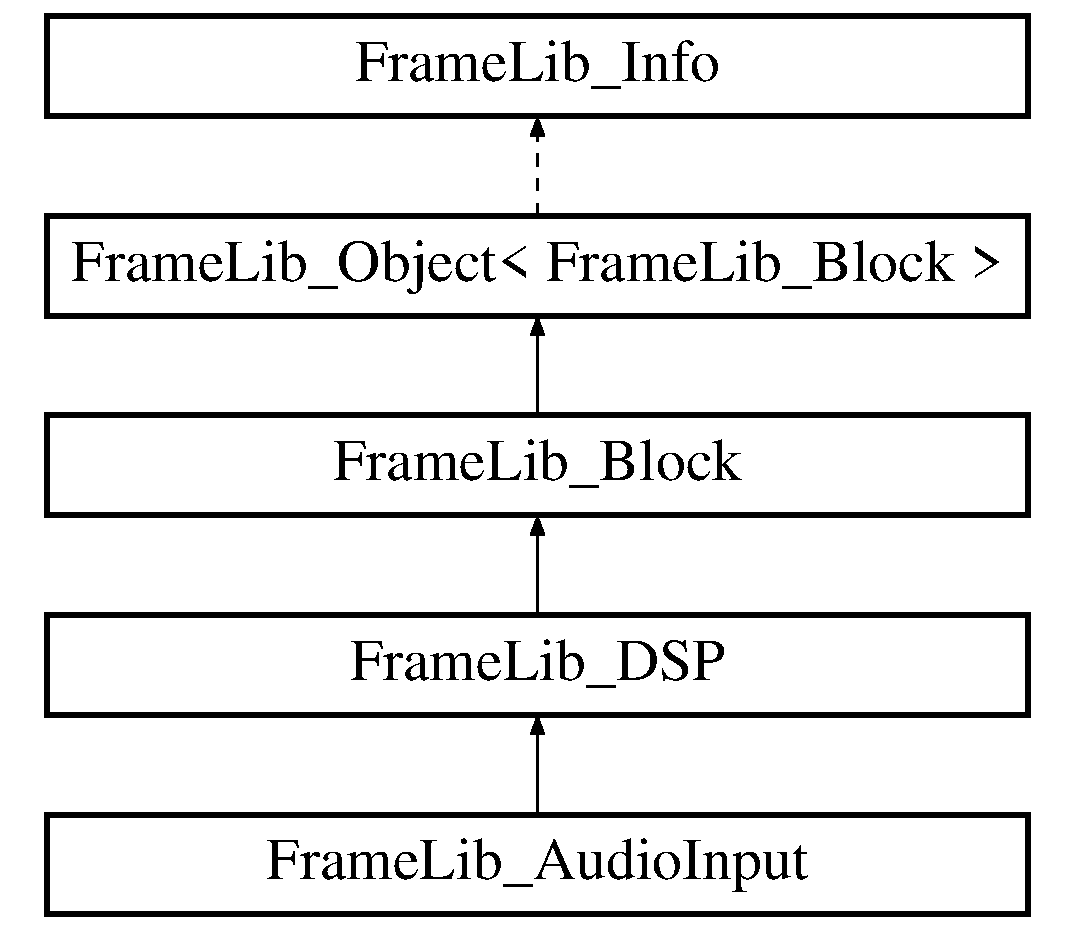
\includegraphics[height=5.000000cm]{class_frame_lib___audio_input}
\end{center}
\end{figure}
\subsection*{Public Member Functions}
\begin{DoxyCompactItemize}
\item 
\hyperlink{class_frame_lib___audio_input_a5fcacfa38f33f949e76d046117835ace}{Frame\+Lib\+\_\+\+Audio\+Input} (\hyperlink{class_frame_lib___context}{Frame\+Lib\+\_\+\+Context} context, void $\ast$owner, \hyperlink{class_frame_lib___parameters_1_1_info}{Frame\+Lib\+\_\+\+Parameters\+::\+Info} $\ast$info, unsigned long n\+Ins=0, unsigned long n\+Outs=0, unsigned long n\+Audio\+Ins=0)
\end{DoxyCompactItemize}
\subsection*{Static Public Member Functions}
\begin{DoxyCompactItemize}
\item 
static \hyperlink{_frame_lib___types_8h_a842c5e2e69277690b064bf363c017980}{Object\+Type} \hyperlink{class_frame_lib___audio_input_a8a6f94b1530b3fd5b604d3151fad5220}{get\+Type} ()
\item 
static bool \hyperlink{class_frame_lib___audio_input_ad0586445ce01e95a3c832ecdc5dc1200}{handles\+Audio} ()
\end{DoxyCompactItemize}
\subsection*{Protected Member Functions}
\begin{DoxyCompactItemize}
\item 
virtual \hyperlink{struct_frame_lib___d_s_p_1_1_scheduler_info}{Scheduler\+Info} \hyperlink{class_frame_lib___audio_input_aaa16c1cb4486b196362b5edf1c60f689}{schedule} (bool new\+Frame, bool no\+Advance)
\end{DoxyCompactItemize}
\subsection*{Additional Inherited Members}


\subsection{Constructor \& Destructor Documentation}
\mbox{\Hypertarget{class_frame_lib___audio_input_a5fcacfa38f33f949e76d046117835ace}\label{class_frame_lib___audio_input_a5fcacfa38f33f949e76d046117835ace}} 
\index{Frame\+Lib\+\_\+\+Audio\+Input@{Frame\+Lib\+\_\+\+Audio\+Input}!Frame\+Lib\+\_\+\+Audio\+Input@{Frame\+Lib\+\_\+\+Audio\+Input}}
\index{Frame\+Lib\+\_\+\+Audio\+Input@{Frame\+Lib\+\_\+\+Audio\+Input}!Frame\+Lib\+\_\+\+Audio\+Input@{Frame\+Lib\+\_\+\+Audio\+Input}}
\subsubsection{\texorpdfstring{Frame\+Lib\+\_\+\+Audio\+Input()}{FrameLib\_AudioInput()}}
{\footnotesize\ttfamily Frame\+Lib\+\_\+\+Audio\+Input\+::\+Frame\+Lib\+\_\+\+Audio\+Input (\begin{DoxyParamCaption}\item[{\hyperlink{class_frame_lib___context}{Frame\+Lib\+\_\+\+Context}}]{context,  }\item[{void $\ast$}]{owner,  }\item[{\hyperlink{class_frame_lib___parameters_1_1_info}{Frame\+Lib\+\_\+\+Parameters\+::\+Info} $\ast$}]{info,  }\item[{unsigned long}]{n\+Ins = {\ttfamily 0},  }\item[{unsigned long}]{n\+Outs = {\ttfamily 0},  }\item[{unsigned long}]{n\+Audio\+Ins = {\ttfamily 0} }\end{DoxyParamCaption})\hspace{0.3cm}{\ttfamily [inline]}}



\subsection{Member Function Documentation}
\mbox{\Hypertarget{class_frame_lib___audio_input_a8a6f94b1530b3fd5b604d3151fad5220}\label{class_frame_lib___audio_input_a8a6f94b1530b3fd5b604d3151fad5220}} 
\index{Frame\+Lib\+\_\+\+Audio\+Input@{Frame\+Lib\+\_\+\+Audio\+Input}!get\+Type@{get\+Type}}
\index{get\+Type@{get\+Type}!Frame\+Lib\+\_\+\+Audio\+Input@{Frame\+Lib\+\_\+\+Audio\+Input}}
\subsubsection{\texorpdfstring{get\+Type()}{getType()}}
{\footnotesize\ttfamily static \hyperlink{_frame_lib___types_8h_a842c5e2e69277690b064bf363c017980}{Object\+Type} Frame\+Lib\+\_\+\+Audio\+Input\+::get\+Type (\begin{DoxyParamCaption}{ }\end{DoxyParamCaption})\hspace{0.3cm}{\ttfamily [inline]}, {\ttfamily [static]}}

\mbox{\Hypertarget{class_frame_lib___audio_input_ad0586445ce01e95a3c832ecdc5dc1200}\label{class_frame_lib___audio_input_ad0586445ce01e95a3c832ecdc5dc1200}} 
\index{Frame\+Lib\+\_\+\+Audio\+Input@{Frame\+Lib\+\_\+\+Audio\+Input}!handles\+Audio@{handles\+Audio}}
\index{handles\+Audio@{handles\+Audio}!Frame\+Lib\+\_\+\+Audio\+Input@{Frame\+Lib\+\_\+\+Audio\+Input}}
\subsubsection{\texorpdfstring{handles\+Audio()}{handlesAudio()}}
{\footnotesize\ttfamily static bool Frame\+Lib\+\_\+\+Audio\+Input\+::handles\+Audio (\begin{DoxyParamCaption}{ }\end{DoxyParamCaption})\hspace{0.3cm}{\ttfamily [inline]}, {\ttfamily [static]}}

\mbox{\Hypertarget{class_frame_lib___audio_input_aaa16c1cb4486b196362b5edf1c60f689}\label{class_frame_lib___audio_input_aaa16c1cb4486b196362b5edf1c60f689}} 
\index{Frame\+Lib\+\_\+\+Audio\+Input@{Frame\+Lib\+\_\+\+Audio\+Input}!schedule@{schedule}}
\index{schedule@{schedule}!Frame\+Lib\+\_\+\+Audio\+Input@{Frame\+Lib\+\_\+\+Audio\+Input}}
\subsubsection{\texorpdfstring{schedule()}{schedule()}}
{\footnotesize\ttfamily virtual \hyperlink{struct_frame_lib___d_s_p_1_1_scheduler_info}{Scheduler\+Info} Frame\+Lib\+\_\+\+Audio\+Input\+::schedule (\begin{DoxyParamCaption}\item[{bool}]{new\+Frame,  }\item[{bool}]{no\+Advance }\end{DoxyParamCaption})\hspace{0.3cm}{\ttfamily [inline]}, {\ttfamily [protected]}, {\ttfamily [virtual]}}



Implements \hyperlink{class_frame_lib___d_s_p}{Frame\+Lib\+\_\+\+D\+SP}.



The documentation for this class was generated from the following file\+:\begin{DoxyCompactItemize}
\item 
/\+Users/alexharker/\+Documents/\+Max Externals/\+Frame\+Lib/\+Frame\+Lib\+\_\+\+Framework/\hyperlink{_frame_lib___d_s_p_8h}{Frame\+Lib\+\_\+\+D\+S\+P.\+h}\end{DoxyCompactItemize}

\hypertarget{class_frame_lib___audio_output}{}\section{Frame\+Lib\+\_\+\+Audio\+Output Class Reference}
\label{class_frame_lib___audio_output}\index{Frame\+Lib\+\_\+\+Audio\+Output@{Frame\+Lib\+\_\+\+Audio\+Output}}


{\ttfamily \#include $<$Frame\+Lib\+\_\+\+D\+S\+P.\+h$>$}

Inheritance diagram for Frame\+Lib\+\_\+\+Audio\+Output\+:\begin{figure}[H]
\begin{center}
\leavevmode
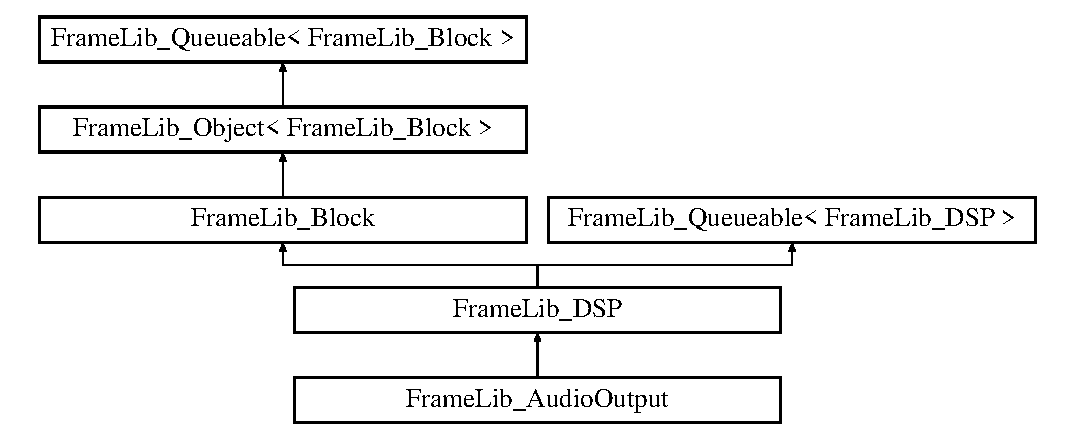
\includegraphics[height=5.000000cm]{class_frame_lib___audio_output}
\end{center}
\end{figure}
\subsection*{Public Member Functions}
\begin{DoxyCompactItemize}
\item 
\hyperlink{class_frame_lib___audio_output_aa63caeed1cdb5887b1a81f1de2b300a1}{Frame\+Lib\+\_\+\+Audio\+Output} (\hyperlink{class_frame_lib___context}{Frame\+Lib\+\_\+\+Context} context, void $\ast$owner, \hyperlink{class_frame_lib___parameters_1_1_info}{Frame\+Lib\+\_\+\+Parameters\+::\+Info} $\ast$info, unsigned long n\+Ins=0, unsigned long n\+Outs=0, unsigned long n\+Audio\+Outs=0)
\end{DoxyCompactItemize}
\subsection*{Static Public Member Functions}
\begin{DoxyCompactItemize}
\item 
static \hyperlink{_frame_lib___types_8h_a842c5e2e69277690b064bf363c017980}{Object\+Type} \hyperlink{class_frame_lib___audio_output_a99908793774ac5046c3e369bc9a19259}{get\+Type} ()
\item 
static bool \hyperlink{class_frame_lib___audio_output_a394659d38e6e48418faf75bbae4cbc01}{handles\+Audio} ()
\end{DoxyCompactItemize}
\subsection*{Protected Member Functions}
\begin{DoxyCompactItemize}
\item 
virtual \hyperlink{struct_frame_lib___d_s_p_1_1_scheduler_info}{Scheduler\+Info} \hyperlink{class_frame_lib___audio_output_a39e97cc3e92147465cf1f6c267de185d}{schedule} (bool new\+Frame, bool no\+Advance)
\end{DoxyCompactItemize}
\subsection*{Additional Inherited Members}


\subsection{Constructor \& Destructor Documentation}
\mbox{\Hypertarget{class_frame_lib___audio_output_aa63caeed1cdb5887b1a81f1de2b300a1}\label{class_frame_lib___audio_output_aa63caeed1cdb5887b1a81f1de2b300a1}} 
\index{Frame\+Lib\+\_\+\+Audio\+Output@{Frame\+Lib\+\_\+\+Audio\+Output}!Frame\+Lib\+\_\+\+Audio\+Output@{Frame\+Lib\+\_\+\+Audio\+Output}}
\index{Frame\+Lib\+\_\+\+Audio\+Output@{Frame\+Lib\+\_\+\+Audio\+Output}!Frame\+Lib\+\_\+\+Audio\+Output@{Frame\+Lib\+\_\+\+Audio\+Output}}
\subsubsection{\texorpdfstring{Frame\+Lib\+\_\+\+Audio\+Output()}{FrameLib\_AudioOutput()}}
{\footnotesize\ttfamily Frame\+Lib\+\_\+\+Audio\+Output\+::\+Frame\+Lib\+\_\+\+Audio\+Output (\begin{DoxyParamCaption}\item[{\hyperlink{class_frame_lib___context}{Frame\+Lib\+\_\+\+Context}}]{context,  }\item[{void $\ast$}]{owner,  }\item[{\hyperlink{class_frame_lib___parameters_1_1_info}{Frame\+Lib\+\_\+\+Parameters\+::\+Info} $\ast$}]{info,  }\item[{unsigned long}]{n\+Ins = {\ttfamily 0},  }\item[{unsigned long}]{n\+Outs = {\ttfamily 0},  }\item[{unsigned long}]{n\+Audio\+Outs = {\ttfamily 0} }\end{DoxyParamCaption})\hspace{0.3cm}{\ttfamily [inline]}}



\subsection{Member Function Documentation}
\mbox{\Hypertarget{class_frame_lib___audio_output_a99908793774ac5046c3e369bc9a19259}\label{class_frame_lib___audio_output_a99908793774ac5046c3e369bc9a19259}} 
\index{Frame\+Lib\+\_\+\+Audio\+Output@{Frame\+Lib\+\_\+\+Audio\+Output}!get\+Type@{get\+Type}}
\index{get\+Type@{get\+Type}!Frame\+Lib\+\_\+\+Audio\+Output@{Frame\+Lib\+\_\+\+Audio\+Output}}
\subsubsection{\texorpdfstring{get\+Type()}{getType()}}
{\footnotesize\ttfamily static \hyperlink{_frame_lib___types_8h_a842c5e2e69277690b064bf363c017980}{Object\+Type} Frame\+Lib\+\_\+\+Audio\+Output\+::get\+Type (\begin{DoxyParamCaption}{ }\end{DoxyParamCaption})\hspace{0.3cm}{\ttfamily [inline]}, {\ttfamily [static]}}

\mbox{\Hypertarget{class_frame_lib___audio_output_a394659d38e6e48418faf75bbae4cbc01}\label{class_frame_lib___audio_output_a394659d38e6e48418faf75bbae4cbc01}} 
\index{Frame\+Lib\+\_\+\+Audio\+Output@{Frame\+Lib\+\_\+\+Audio\+Output}!handles\+Audio@{handles\+Audio}}
\index{handles\+Audio@{handles\+Audio}!Frame\+Lib\+\_\+\+Audio\+Output@{Frame\+Lib\+\_\+\+Audio\+Output}}
\subsubsection{\texorpdfstring{handles\+Audio()}{handlesAudio()}}
{\footnotesize\ttfamily static bool Frame\+Lib\+\_\+\+Audio\+Output\+::handles\+Audio (\begin{DoxyParamCaption}{ }\end{DoxyParamCaption})\hspace{0.3cm}{\ttfamily [inline]}, {\ttfamily [static]}}

\mbox{\Hypertarget{class_frame_lib___audio_output_a39e97cc3e92147465cf1f6c267de185d}\label{class_frame_lib___audio_output_a39e97cc3e92147465cf1f6c267de185d}} 
\index{Frame\+Lib\+\_\+\+Audio\+Output@{Frame\+Lib\+\_\+\+Audio\+Output}!schedule@{schedule}}
\index{schedule@{schedule}!Frame\+Lib\+\_\+\+Audio\+Output@{Frame\+Lib\+\_\+\+Audio\+Output}}
\subsubsection{\texorpdfstring{schedule()}{schedule()}}
{\footnotesize\ttfamily virtual \hyperlink{struct_frame_lib___d_s_p_1_1_scheduler_info}{Scheduler\+Info} Frame\+Lib\+\_\+\+Audio\+Output\+::schedule (\begin{DoxyParamCaption}\item[{bool}]{new\+Frame,  }\item[{bool}]{no\+Advance }\end{DoxyParamCaption})\hspace{0.3cm}{\ttfamily [inline]}, {\ttfamily [protected]}, {\ttfamily [virtual]}}



Implements \hyperlink{class_frame_lib___d_s_p}{Frame\+Lib\+\_\+\+D\+SP}.



The documentation for this class was generated from the following file\+:\begin{DoxyCompactItemize}
\item 
/\+Users/alexharker/\+Documents/\+Max Externals/\+Frame\+Lib/\+Frame\+Lib\+\_\+\+Framework/\hyperlink{_frame_lib___d_s_p_8h}{Frame\+Lib\+\_\+\+D\+S\+P.\+h}\end{DoxyCompactItemize}

\hypertarget{class_frame_lib___block}{}\section{Frame\+Lib\+\_\+\+Block Class Reference}
\label{class_frame_lib___block}\index{Frame\+Lib\+\_\+\+Block@{Frame\+Lib\+\_\+\+Block}}


{\ttfamily \#include $<$Frame\+Lib\+\_\+\+Object.\+h$>$}

Inheritance diagram for Frame\+Lib\+\_\+\+Block\+:\begin{figure}[H]
\begin{center}
\leavevmode
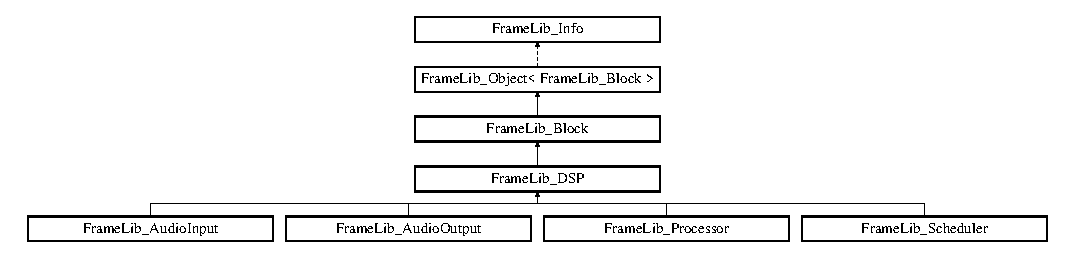
\includegraphics[height=3.017241cm]{class_frame_lib___block}
\end{center}
\end{figure}
\subsection*{Public Member Functions}
\begin{DoxyCompactItemize}
\item 
\hyperlink{class_frame_lib___block_ab56169e5918fe77c1cfa7ddd0a6520a3}{Frame\+Lib\+\_\+\+Block} (\hyperlink{_frame_lib___types_8h_a842c5e2e69277690b064bf363c017980}{Object\+Type} type)
\item 
virtual \hyperlink{class_frame_lib___block_a17c0048595334cb8d63abfcbb77c980d}{$\sim$\+Frame\+Lib\+\_\+\+Block} ()
\item 
virtual void \hyperlink{class_frame_lib___block_a58ad49f15453e8214a298ef0992b00a1}{add\+Connection} (class \hyperlink{class_frame_lib___d_s_p}{Frame\+Lib\+\_\+\+D\+SP} $\ast$object, unsigned long out\+Idx, unsigned long in\+Idx)=0
\item 
virtual void \hyperlink{class_frame_lib___block_a88e998ec661b9afd001e40e68bb52f61}{add\+Connection} (\hyperlink{class_frame_lib___block}{Frame\+Lib\+\_\+\+Block} $\ast$object, unsigned long out\+Idx, unsigned long in\+Idx)
\end{DoxyCompactItemize}
\subsection*{Protected Member Functions}
\begin{DoxyCompactItemize}
\item 
virtual class \hyperlink{class_frame_lib___d_s_p}{Frame\+Lib\+\_\+\+D\+SP} $\ast$ \hyperlink{class_frame_lib___block_a9e8bb5dcd9954618de9a8e3ad27c16a9}{get\+Output\+Object} (unsigned long out\+Idx)=0
\end{DoxyCompactItemize}
\subsection*{Additional Inherited Members}


\subsection{Constructor \& Destructor Documentation}
\mbox{\Hypertarget{class_frame_lib___block_ab56169e5918fe77c1cfa7ddd0a6520a3}\label{class_frame_lib___block_ab56169e5918fe77c1cfa7ddd0a6520a3}} 
\index{Frame\+Lib\+\_\+\+Block@{Frame\+Lib\+\_\+\+Block}!Frame\+Lib\+\_\+\+Block@{Frame\+Lib\+\_\+\+Block}}
\index{Frame\+Lib\+\_\+\+Block@{Frame\+Lib\+\_\+\+Block}!Frame\+Lib\+\_\+\+Block@{Frame\+Lib\+\_\+\+Block}}
\subsubsection{\texorpdfstring{Frame\+Lib\+\_\+\+Block()}{FrameLib\_Block()}}
{\footnotesize\ttfamily Frame\+Lib\+\_\+\+Block\+::\+Frame\+Lib\+\_\+\+Block (\begin{DoxyParamCaption}\item[{\hyperlink{_frame_lib___types_8h_a842c5e2e69277690b064bf363c017980}{Object\+Type}}]{type }\end{DoxyParamCaption})\hspace{0.3cm}{\ttfamily [inline]}}

\mbox{\Hypertarget{class_frame_lib___block_a17c0048595334cb8d63abfcbb77c980d}\label{class_frame_lib___block_a17c0048595334cb8d63abfcbb77c980d}} 
\index{Frame\+Lib\+\_\+\+Block@{Frame\+Lib\+\_\+\+Block}!````~Frame\+Lib\+\_\+\+Block@{$\sim$\+Frame\+Lib\+\_\+\+Block}}
\index{````~Frame\+Lib\+\_\+\+Block@{$\sim$\+Frame\+Lib\+\_\+\+Block}!Frame\+Lib\+\_\+\+Block@{Frame\+Lib\+\_\+\+Block}}
\subsubsection{\texorpdfstring{$\sim$\+Frame\+Lib\+\_\+\+Block()}{~FrameLib\_Block()}}
{\footnotesize\ttfamily virtual Frame\+Lib\+\_\+\+Block\+::$\sim$\+Frame\+Lib\+\_\+\+Block (\begin{DoxyParamCaption}{ }\end{DoxyParamCaption})\hspace{0.3cm}{\ttfamily [inline]}, {\ttfamily [virtual]}}



\subsection{Member Function Documentation}
\mbox{\Hypertarget{class_frame_lib___block_a58ad49f15453e8214a298ef0992b00a1}\label{class_frame_lib___block_a58ad49f15453e8214a298ef0992b00a1}} 
\index{Frame\+Lib\+\_\+\+Block@{Frame\+Lib\+\_\+\+Block}!add\+Connection@{add\+Connection}}
\index{add\+Connection@{add\+Connection}!Frame\+Lib\+\_\+\+Block@{Frame\+Lib\+\_\+\+Block}}
\subsubsection{\texorpdfstring{add\+Connection()}{addConnection()}\hspace{0.1cm}{\footnotesize\ttfamily [1/2]}}
{\footnotesize\ttfamily virtual void Frame\+Lib\+\_\+\+Block\+::add\+Connection (\begin{DoxyParamCaption}\item[{class \hyperlink{class_frame_lib___d_s_p}{Frame\+Lib\+\_\+\+D\+SP} $\ast$}]{object,  }\item[{unsigned long}]{out\+Idx,  }\item[{unsigned long}]{in\+Idx }\end{DoxyParamCaption})\hspace{0.3cm}{\ttfamily [pure virtual]}}



Implemented in \hyperlink{class_frame_lib___d_s_p_a835fc24bc4224279fa53b15bde7a824f}{Frame\+Lib\+\_\+\+D\+SP}.

\mbox{\Hypertarget{class_frame_lib___block_a88e998ec661b9afd001e40e68bb52f61}\label{class_frame_lib___block_a88e998ec661b9afd001e40e68bb52f61}} 
\index{Frame\+Lib\+\_\+\+Block@{Frame\+Lib\+\_\+\+Block}!add\+Connection@{add\+Connection}}
\index{add\+Connection@{add\+Connection}!Frame\+Lib\+\_\+\+Block@{Frame\+Lib\+\_\+\+Block}}
\subsubsection{\texorpdfstring{add\+Connection()}{addConnection()}\hspace{0.1cm}{\footnotesize\ttfamily [2/2]}}
{\footnotesize\ttfamily virtual void Frame\+Lib\+\_\+\+Block\+::add\+Connection (\begin{DoxyParamCaption}\item[{\hyperlink{class_frame_lib___block}{Frame\+Lib\+\_\+\+Block} $\ast$}]{object,  }\item[{unsigned long}]{out\+Idx,  }\item[{unsigned long}]{in\+Idx }\end{DoxyParamCaption})\hspace{0.3cm}{\ttfamily [inline]}, {\ttfamily [virtual]}}



Implements \hyperlink{class_frame_lib___object_ab276c500466359bb43494ff2b7c94cc6}{Frame\+Lib\+\_\+\+Object$<$ Frame\+Lib\+\_\+\+Block $>$}.

\mbox{\Hypertarget{class_frame_lib___block_a9e8bb5dcd9954618de9a8e3ad27c16a9}\label{class_frame_lib___block_a9e8bb5dcd9954618de9a8e3ad27c16a9}} 
\index{Frame\+Lib\+\_\+\+Block@{Frame\+Lib\+\_\+\+Block}!get\+Output\+Object@{get\+Output\+Object}}
\index{get\+Output\+Object@{get\+Output\+Object}!Frame\+Lib\+\_\+\+Block@{Frame\+Lib\+\_\+\+Block}}
\subsubsection{\texorpdfstring{get\+Output\+Object()}{getOutputObject()}}
{\footnotesize\ttfamily virtual class \hyperlink{class_frame_lib___d_s_p}{Frame\+Lib\+\_\+\+D\+SP}$\ast$ Frame\+Lib\+\_\+\+Block\+::get\+Output\+Object (\begin{DoxyParamCaption}\item[{unsigned long}]{out\+Idx }\end{DoxyParamCaption})\hspace{0.3cm}{\ttfamily [protected]}, {\ttfamily [pure virtual]}}



Implemented in \hyperlink{class_frame_lib___d_s_p_a867822cfa9e3ca491c886cff9f79001d}{Frame\+Lib\+\_\+\+D\+SP}.



The documentation for this class was generated from the following file\+:\begin{DoxyCompactItemize}
\item 
Frame\+Lib\+\_\+\+Framework/\hyperlink{_frame_lib___object_8h}{Frame\+Lib\+\_\+\+Object.\+h}\end{DoxyCompactItemize}

\hypertarget{class_frame_lib___context}{}\section{Frame\+Lib\+\_\+\+Context Class Reference}
\label{class_frame_lib___context}\index{Frame\+Lib\+\_\+\+Context@{Frame\+Lib\+\_\+\+Context}}


a class used to represent distinct non-\/connectable areas in the host environment.  




{\ttfamily \#include $<$Frame\+Lib\+\_\+\+Context.\+h$>$}

\subsection*{Public Types}
\begin{DoxyCompactItemize}
\item 
using \hyperlink{class_frame_lib___context_a5282f95b5825866bc4bb2aad500ccfa3}{Allocator} = Managed\+Pointer$<$ \hyperlink{class_frame_lib___local_allocator}{Frame\+Lib\+\_\+\+Local\+Allocator}, \&Global\+::get\+Allocator, \&Global\+::release\+Allocator $>$
\item 
using \hyperlink{class_frame_lib___context_aa1c7f3c910b75dbc827a140e5ad33d12}{Processing\+Queue} = Managed\+Pointer$<$ \hyperlink{class_frame_lib___processing_queue}{Frame\+Lib\+\_\+\+Processing\+Queue}, \&Global\+::get\+Processing\+Queue, \&Global\+::release\+Processing\+Queue $>$
\end{DoxyCompactItemize}
\subsection*{Public Member Functions}
\begin{DoxyCompactItemize}
\item 
\hyperlink{class_frame_lib___context_a2cfe1912e3e9d835de291277c8979ed8}{Frame\+Lib\+\_\+\+Context} (\hyperlink{class_frame_lib___global}{Frame\+Lib\+\_\+\+Global} $\ast$global, void $\ast$reference)
\item 
\hyperlink{class_frame_lib___context_a497e6bee6cea6f053ad04086bbc07e50}{operator Frame\+Lib\+\_\+\+Error\+Reporter \&} ()
\end{DoxyCompactItemize}
\subsection*{Friends}
\begin{DoxyCompactItemize}
\item 
bool \hyperlink{class_frame_lib___context_ab0382454ba28ee3ff302be24ffc861c0}{operator==} (const \hyperlink{class_frame_lib___context}{Frame\+Lib\+\_\+\+Context} \&a, const \hyperlink{class_frame_lib___context}{Frame\+Lib\+\_\+\+Context} \&b)
\item 
bool \hyperlink{class_frame_lib___context_a7aed82ce3d334858032a3c45e3c70169}{operator!=} (const \hyperlink{class_frame_lib___context}{Frame\+Lib\+\_\+\+Context} \&a, const \hyperlink{class_frame_lib___context}{Frame\+Lib\+\_\+\+Context} \&b)
\end{DoxyCompactItemize}


\subsection{Detailed Description}
a class used to represent distinct non-\/connectable areas in the host environment. 

The context acts as a proxy to \hyperlink{class_frame_lib___global}{Frame\+Lib\+\_\+\+Global}, and contains a suitable pointer reference to the context in the host environment. Resources for each context are held in the global object, and the context is passed as a parameter when creating any Frame\+Lib object. 

\subsection{Member Typedef Documentation}
\mbox{\Hypertarget{class_frame_lib___context_a5282f95b5825866bc4bb2aad500ccfa3}\label{class_frame_lib___context_a5282f95b5825866bc4bb2aad500ccfa3}} 
\index{Frame\+Lib\+\_\+\+Context@{Frame\+Lib\+\_\+\+Context}!Allocator@{Allocator}}
\index{Allocator@{Allocator}!Frame\+Lib\+\_\+\+Context@{Frame\+Lib\+\_\+\+Context}}
\subsubsection{\texorpdfstring{Allocator}{Allocator}}
{\footnotesize\ttfamily using \hyperlink{class_frame_lib___context_a5282f95b5825866bc4bb2aad500ccfa3}{Frame\+Lib\+\_\+\+Context\+::\+Allocator} =  Managed\+Pointer$<$\hyperlink{class_frame_lib___local_allocator}{Frame\+Lib\+\_\+\+Local\+Allocator}, \&Global\+::get\+Allocator, \&Global\+::release\+Allocator$>$}

\mbox{\Hypertarget{class_frame_lib___context_aa1c7f3c910b75dbc827a140e5ad33d12}\label{class_frame_lib___context_aa1c7f3c910b75dbc827a140e5ad33d12}} 
\index{Frame\+Lib\+\_\+\+Context@{Frame\+Lib\+\_\+\+Context}!Processing\+Queue@{Processing\+Queue}}
\index{Processing\+Queue@{Processing\+Queue}!Frame\+Lib\+\_\+\+Context@{Frame\+Lib\+\_\+\+Context}}
\subsubsection{\texorpdfstring{Processing\+Queue}{ProcessingQueue}}
{\footnotesize\ttfamily using \hyperlink{class_frame_lib___context_aa1c7f3c910b75dbc827a140e5ad33d12}{Frame\+Lib\+\_\+\+Context\+::\+Processing\+Queue} =  Managed\+Pointer$<$\hyperlink{class_frame_lib___processing_queue}{Frame\+Lib\+\_\+\+Processing\+Queue}, \&Global\+::get\+Processing\+Queue, \&Global\+::release\+Processing\+Queue$>$}



\subsection{Constructor \& Destructor Documentation}
\mbox{\Hypertarget{class_frame_lib___context_a2cfe1912e3e9d835de291277c8979ed8}\label{class_frame_lib___context_a2cfe1912e3e9d835de291277c8979ed8}} 
\index{Frame\+Lib\+\_\+\+Context@{Frame\+Lib\+\_\+\+Context}!Frame\+Lib\+\_\+\+Context@{Frame\+Lib\+\_\+\+Context}}
\index{Frame\+Lib\+\_\+\+Context@{Frame\+Lib\+\_\+\+Context}!Frame\+Lib\+\_\+\+Context@{Frame\+Lib\+\_\+\+Context}}
\subsubsection{\texorpdfstring{Frame\+Lib\+\_\+\+Context()}{FrameLib\_Context()}}
{\footnotesize\ttfamily Frame\+Lib\+\_\+\+Context\+::\+Frame\+Lib\+\_\+\+Context (\begin{DoxyParamCaption}\item[{\hyperlink{class_frame_lib___global}{Frame\+Lib\+\_\+\+Global} $\ast$}]{global,  }\item[{void $\ast$}]{reference }\end{DoxyParamCaption})\hspace{0.3cm}{\ttfamily [inline]}}



\subsection{Member Function Documentation}
\mbox{\Hypertarget{class_frame_lib___context_a497e6bee6cea6f053ad04086bbc07e50}\label{class_frame_lib___context_a497e6bee6cea6f053ad04086bbc07e50}} 
\index{Frame\+Lib\+\_\+\+Context@{Frame\+Lib\+\_\+\+Context}!operator Frame\+Lib\+\_\+\+Error\+Reporter \&@{operator Frame\+Lib\+\_\+\+Error\+Reporter \&}}
\index{operator Frame\+Lib\+\_\+\+Error\+Reporter \&@{operator Frame\+Lib\+\_\+\+Error\+Reporter \&}!Frame\+Lib\+\_\+\+Context@{Frame\+Lib\+\_\+\+Context}}
\subsubsection{\texorpdfstring{operator Frame\+Lib\+\_\+\+Error\+Reporter \&()}{operator FrameLib\_ErrorReporter \&()}}
{\footnotesize\ttfamily Frame\+Lib\+\_\+\+Context\+::operator \hyperlink{class_frame_lib___error_reporter}{Frame\+Lib\+\_\+\+Error\+Reporter} \& (\begin{DoxyParamCaption}{ }\end{DoxyParamCaption})\hspace{0.3cm}{\ttfamily [inline]}}



\subsection{Friends And Related Function Documentation}
\mbox{\Hypertarget{class_frame_lib___context_a7aed82ce3d334858032a3c45e3c70169}\label{class_frame_lib___context_a7aed82ce3d334858032a3c45e3c70169}} 
\index{Frame\+Lib\+\_\+\+Context@{Frame\+Lib\+\_\+\+Context}!operator"!=@{operator"!=}}
\index{operator"!=@{operator"!=}!Frame\+Lib\+\_\+\+Context@{Frame\+Lib\+\_\+\+Context}}
\subsubsection{\texorpdfstring{operator"!=}{operator!=}}
{\footnotesize\ttfamily bool operator!= (\begin{DoxyParamCaption}\item[{const \hyperlink{class_frame_lib___context}{Frame\+Lib\+\_\+\+Context} \&}]{a,  }\item[{const \hyperlink{class_frame_lib___context}{Frame\+Lib\+\_\+\+Context} \&}]{b }\end{DoxyParamCaption})\hspace{0.3cm}{\ttfamily [friend]}}

\mbox{\Hypertarget{class_frame_lib___context_ab0382454ba28ee3ff302be24ffc861c0}\label{class_frame_lib___context_ab0382454ba28ee3ff302be24ffc861c0}} 
\index{Frame\+Lib\+\_\+\+Context@{Frame\+Lib\+\_\+\+Context}!operator==@{operator==}}
\index{operator==@{operator==}!Frame\+Lib\+\_\+\+Context@{Frame\+Lib\+\_\+\+Context}}
\subsubsection{\texorpdfstring{operator==}{operator==}}
{\footnotesize\ttfamily bool operator== (\begin{DoxyParamCaption}\item[{const \hyperlink{class_frame_lib___context}{Frame\+Lib\+\_\+\+Context} \&}]{a,  }\item[{const \hyperlink{class_frame_lib___context}{Frame\+Lib\+\_\+\+Context} \&}]{b }\end{DoxyParamCaption})\hspace{0.3cm}{\ttfamily [friend]}}



The documentation for this class was generated from the following file\+:\begin{DoxyCompactItemize}
\item 
/\+Users/alexharker/\+Documents/\+Max Externals/\+Frame\+Lib/\+Frame\+Lib\+\_\+\+Framework/\hyperlink{_frame_lib___context_8h}{Frame\+Lib\+\_\+\+Context.\+h}\end{DoxyCompactItemize}

\hypertarget{class_frame_lib___d_s_p}{}\section{Frame\+Lib\+\_\+\+D\+SP Class Reference}
\label{class_frame_lib___d_s_p}\index{Frame\+Lib\+\_\+\+D\+SP@{Frame\+Lib\+\_\+\+D\+SP}}


an abstract class containing the core of the D\+SP processing system, which handles single-\/stream scheduling.  




{\ttfamily \#include $<$Frame\+Lib\+\_\+\+D\+S\+P.\+h$>$}

Inheritance diagram for Frame\+Lib\+\_\+\+D\+SP\+:\begin{figure}[H]
\begin{center}
\leavevmode
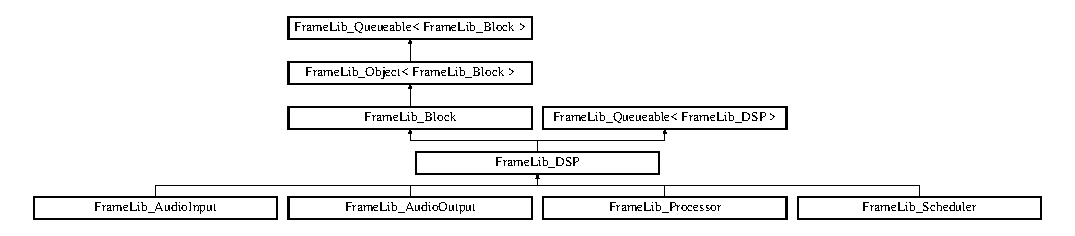
\includegraphics[height=2.723735cm]{class_frame_lib___d_s_p}
\end{center}
\end{figure}
\subsection*{Classes}
\begin{DoxyCompactItemize}
\item 
struct \hyperlink{struct_frame_lib___d_s_p_1_1_scheduler_info}{Scheduler\+Info}
\begin{DoxyCompactList}\small\item\em an struct for returning scheduling info from the schedule() method. \end{DoxyCompactList}\end{DoxyCompactItemize}
\subsection*{Public Member Functions}
\begin{DoxyCompactItemize}
\item 
\hyperlink{class_frame_lib___d_s_p_a05ee5380cce6fa82c2b91c3f08693cc0}{Frame\+Lib\+\_\+\+D\+SP} (\hyperlink{_frame_lib___types_8h_a842c5e2e69277690b064bf363c017980}{Object\+Type} type, \hyperlink{class_frame_lib___context}{Frame\+Lib\+\_\+\+Context} context, \hyperlink{struct_frame_lib___proxy}{Frame\+Lib\+\_\+\+Proxy} $\ast$proxy, \hyperlink{class_frame_lib___parameters_1_1_info}{Frame\+Lib\+\_\+\+Parameters\+::\+Info} $\ast$info, unsigned long n\+Ins, unsigned long n\+Outs, unsigned long n\+Audio\+Chans=0)
\item 
\hyperlink{class_frame_lib___d_s_p_a2cf489678b72fe7e46956e69fac182ed}{$\sim$\+Frame\+Lib\+\_\+\+D\+SP} ()
\item 
\hyperlink{class_frame_lib___d_s_p_afd70a8e76dc70ac0fbe4d3f9a7a5beaf}{Frame\+Lib\+\_\+\+D\+SP} (const \hyperlink{class_frame_lib___d_s_p}{Frame\+Lib\+\_\+\+D\+SP} \&)=delete
\item 
\hyperlink{class_frame_lib___d_s_p}{Frame\+Lib\+\_\+\+D\+SP} \& \hyperlink{class_frame_lib___d_s_p_ab6c001c4768ed250fe9b223de1dc4d5f}{operator=} (const \hyperlink{class_frame_lib___d_s_p}{Frame\+Lib\+\_\+\+D\+SP} \&)=delete
\item 
void \hyperlink{class_frame_lib___d_s_p_a426afa0cf5d8f5c625619da2ccbf9be4}{set\+Fixed\+Input} (unsigned long idx, double $\ast$input, unsigned long size) final
\item 
const double $\ast$ \hyperlink{class_frame_lib___d_s_p_aabcf3bae08ab571f455f08bd7cf5e625}{get\+Fixed\+Input} (unsigned long idx, unsigned long $\ast$size) final
\item 
void \hyperlink{class_frame_lib___d_s_p_a106b275882df26129c1af0ab89487b65}{block\+Update} (const double $\ast$const $\ast$ins, double $\ast$$\ast$outs, unsigned long \hyperlink{_frame_lib___memory_8cpp_a8ef7d53a4cac28bf580a61f265fcaaa6}{block\+Size}) final
\item 
void \hyperlink{class_frame_lib___d_s_p_a0b0edaaaa82b80f3800918283a6a46f0}{reset} (double sampling\+Rate, unsigned long max\+Block\+Size) final
\item 
const \hyperlink{class_frame_lib___parameters}{Frame\+Lib\+\_\+\+Parameters} $\ast$ \hyperlink{class_frame_lib___d_s_p_ab1b692f7fe4340b7837319ceed334f02}{get\+Parameters} () const final
\item 
\hyperlink{_frame_lib___types_8h_ad495a9f61af7fff07d7e97979d1ab854}{Frame\+Type} \hyperlink{class_frame_lib___d_s_p_abbe65d74de56ab71e7fba34380bd19dc}{input\+Type} (unsigned long idx) const final
\item 
\hyperlink{_frame_lib___types_8h_ad495a9f61af7fff07d7e97979d1ab854}{Frame\+Type} \hyperlink{class_frame_lib___d_s_p_a14154f7fe15aa51b683e56e8a368b9ad}{output\+Type} (unsigned long idx) const final
\item 
void \hyperlink{class_frame_lib___d_s_p_a6584230fa17c0b76a045fd1ec99f0482}{auto\+Ordering\+Connections} () final
\item 
void \hyperlink{class_frame_lib___d_s_p_a8c9843103d691ed57e3e265528f575be}{clear\+Auto\+Ordering\+Connections} () final
\end{DoxyCompactItemize}
\subsection*{Protected Member Functions}
\begin{DoxyCompactItemize}
\item 
void \hyperlink{class_frame_lib___d_s_p_a3d184baeb7b55fa099cb9c4a7393c70c}{set\+IO} (unsigned long n\+Ins, unsigned long n\+Outs, unsigned long n\+Audio\+Chans=0)
\item 
void \hyperlink{class_frame_lib___d_s_p_ae88480e015d70507fd1f7853fc17ffa2}{set\+Input\+Mode} (unsigned long idx, bool update, bool trigger, bool switchable, \hyperlink{_frame_lib___types_8h_ad495a9f61af7fff07d7e97979d1ab854}{Frame\+Type} type=\hyperlink{_frame_lib___types_8h_ad495a9f61af7fff07d7e97979d1ab854a4bc2388cbdd721f5039a32f95cd92b03}{k\+Frame\+Normal})
\item 
void \hyperlink{class_frame_lib___d_s_p_abcbe8babb74a7b85faf8846b4a0ff95f}{set\+Parameter\+Input} (unsigned long idx)
\item 
void \hyperlink{class_frame_lib___d_s_p_aa000b56c19ad1fbdc4f3fe56b0ca762d}{add\+Parameter\+Input} ()
\item 
void \hyperlink{class_frame_lib___d_s_p_a43da3ff5b57b3c1da655b0e6c7c0b37f}{set\+Output\+Type} (unsigned long idx, \hyperlink{_frame_lib___types_8h_ad495a9f61af7fff07d7e97979d1ab854}{Frame\+Type} type)
\item 
void \hyperlink{class_frame_lib___d_s_p_aa2854abee0acbd4e3192a38cb5dc4155}{set\+Current\+Output\+Type} (unsigned long idx, \hyperlink{_frame_lib___types_8h_ad495a9f61af7fff07d7e97979d1ab854}{Frame\+Type} type)
\item 
void \hyperlink{class_frame_lib___d_s_p_a2e3084ad267a330ec021bd558edd3f57}{update\+Trigger} (unsigned long idx, bool trigger)
\item 
bool \hyperlink{class_frame_lib___d_s_p_a13e269a66e0b9fb40ead089530e49eaa}{is\+Trigger} (unsigned long idx) const
\item 
\hyperlink{struct_frame_lib___time_format}{Frame\+Lib\+\_\+\+Time\+Format} \hyperlink{class_frame_lib___d_s_p_a2eedff2474f665b5bf7d2f2fa7a1cdc4}{get\+Frame\+Time} () const
\item 
\hyperlink{struct_frame_lib___time_format}{Frame\+Lib\+\_\+\+Time\+Format} \hyperlink{class_frame_lib___d_s_p_afa420e10b7ea7a300bf106631167cac0}{get\+Valid\+Time} () const
\item 
\hyperlink{struct_frame_lib___time_format}{Frame\+Lib\+\_\+\+Time\+Format} \hyperlink{class_frame_lib___d_s_p_afd7cae225f75c8cd4bd773bf188961b2}{get\+Input\+Time} () const
\item 
\hyperlink{struct_frame_lib___time_format}{Frame\+Lib\+\_\+\+Time\+Format} \hyperlink{class_frame_lib___d_s_p_a5734f973e603be4a85764d5f77fa4004}{get\+Current\+Time} () const
\item 
\hyperlink{struct_frame_lib___time_format}{Frame\+Lib\+\_\+\+Time\+Format} \hyperlink{class_frame_lib___d_s_p_a9c34c56420ff9da196150e8a5307e812}{get\+Block\+Start\+Time} () const
\item 
\hyperlink{struct_frame_lib___time_format}{Frame\+Lib\+\_\+\+Time\+Format} \hyperlink{class_frame_lib___d_s_p_a8cd169b635307807b29f1d02ea23635e}{get\+Block\+End\+Time} () const
\item 
\hyperlink{struct_frame_lib___time_format}{Frame\+Lib\+\_\+\+Time\+Format} \hyperlink{class_frame_lib___d_s_p_a705ddc874bc5643f81a0f71894f1ae0c}{get\+Input\+Frame\+Time} (unsigned long idx) const
\item 
\hyperlink{struct_frame_lib___time_format}{Frame\+Lib\+\_\+\+Time\+Format} \hyperlink{class_frame_lib___d_s_p_a699dda68553ddebd5ca8c70326fb40a5}{get\+Input\+Valid\+Time} (unsigned long idx) const
\item 
void \hyperlink{class_frame_lib___d_s_p_a018be5346f473c3c21d5251d6acb85c7}{request\+Output\+Size} (unsigned long idx, size\+\_\+t size)
\item 
void \hyperlink{class_frame_lib___d_s_p_a7716bc548b4418d6951dbbada499d9d3}{request\+Added\+Output\+Size} (unsigned long idx, size\+\_\+t size)
\item 
bool \hyperlink{class_frame_lib___d_s_p_abbf404ed95c61cfa713c988b10f76202}{allocate\+Outputs} ()
\item 
\hyperlink{_frame_lib___types_8h_ad495a9f61af7fff07d7e97979d1ab854}{Frame\+Type} \hyperlink{class_frame_lib___d_s_p_aba80b7c3546f6e65ab0378628dd2be62}{get\+Input\+Current\+Type} (unsigned long idx) const
\item 
const double $\ast$ \hyperlink{class_frame_lib___d_s_p_aea9dee37e1093a12f7764b12ab430a19}{get\+Input} (unsigned long idx, size\+\_\+t $\ast$size) const
\item 
const \hyperlink{class_frame_lib___parameters_1_1_serial}{Frame\+Lib\+\_\+\+Parameters\+::\+Serial} $\ast$ \hyperlink{class_frame_lib___d_s_p_ae2d4474b0545fcc2cbb5ffcfcf75fc94}{get\+Input} (unsigned long idx) const
\item 
\hyperlink{_frame_lib___types_8h_ad495a9f61af7fff07d7e97979d1ab854}{Frame\+Type} \hyperlink{class_frame_lib___d_s_p_ad870d652a2ce82ca2dee8eba91ad8dd8}{get\+Output\+Current\+Type} (unsigned long idx) const
\item 
double $\ast$ \hyperlink{class_frame_lib___d_s_p_a5d72363b6d5ee02e0c52e499fd28205d}{get\+Output} (unsigned long idx, size\+\_\+t $\ast$size) const
\item 
\hyperlink{class_frame_lib___parameters_1_1_serial}{Frame\+Lib\+\_\+\+Parameters\+::\+Serial} $\ast$ \hyperlink{class_frame_lib___d_s_p_a18dc23246a8c9d67a0cc468e782fd5c3}{get\+Output} (unsigned long idx) const
\item 
void \hyperlink{class_frame_lib___d_s_p_ab2cd55c5a42a4c0489503a95a7ce0853}{prepare\+Copy\+Input\+To\+Output} (unsigned long in\+Idx, unsigned long out\+Idx)
\item 
void \hyperlink{class_frame_lib___d_s_p_abe84c66d723767ef803c58f9ada7a7de}{copy\+Input\+To\+Output} (unsigned long in\+Idx, unsigned long out\+Idx)
\item 
\hyperlink{struct_frame_lib___time_format}{Frame\+Lib\+\_\+\+Time\+Format} \hyperlink{class_frame_lib___d_s_p_a057aba18ccdae856a2d3db37caab496c}{hz\+To\+Samples} (const \hyperlink{struct_frame_lib___time_format}{Frame\+Lib\+\_\+\+Time\+Format} \&a)
\item 
\hyperlink{struct_frame_lib___time_format}{Frame\+Lib\+\_\+\+Time\+Format} \hyperlink{class_frame_lib___d_s_p_a00480b59f602bac240106d31f89cd293}{ms\+To\+Samples} (const \hyperlink{struct_frame_lib___time_format}{Frame\+Lib\+\_\+\+Time\+Format} \&a)
\item 
\hyperlink{struct_frame_lib___time_format}{Frame\+Lib\+\_\+\+Time\+Format} \hyperlink{class_frame_lib___d_s_p_a61da3eb72a4528839fd0dd40a6c36ec6}{seconds\+To\+Samples} (const \hyperlink{struct_frame_lib___time_format}{Frame\+Lib\+\_\+\+Time\+Format} \&a)
\item 
double \hyperlink{class_frame_lib___d_s_p_a56400e47d4d4b9fb579734af888245c7}{hz\+To\+Samples} (double a)
\item 
double \hyperlink{class_frame_lib___d_s_p_a353058bf6287b8677324c64e12b1ae27}{ms\+To\+Samples} (double a)
\item 
double \hyperlink{class_frame_lib___d_s_p_a4162905cc8f98f87081a268e0fbe40e4}{seconds\+To\+Samples} (double a)
\end{DoxyCompactItemize}
\subsection*{Static Protected Member Functions}
\begin{DoxyCompactItemize}
\item 
static void \hyperlink{class_frame_lib___d_s_p_acd722a6a2939ed16f748288901f75119}{copy\+Vector} (double $\ast$output, const double $\ast$input, unsigned long size)
\item 
static void \hyperlink{class_frame_lib___d_s_p_a9da9216b727050afef88ff8e1ec01ba0}{zero\+Vector} (double $\ast$output, unsigned long size)
\item 
static void \hyperlink{class_frame_lib___d_s_p_a53100cc66147cbb05374e5d877ad4bd7}{copy\+Vector\+Extend} (double $\ast$output, const double $\ast$input, unsigned long size\+Out, unsigned long size\+In)
\item 
static void \hyperlink{class_frame_lib___d_s_p_a11ceb4866739ced35e33ce353d293130}{copy\+Vector\+Wrap} (double $\ast$output, const double $\ast$input, unsigned long size\+Out, unsigned long size\+In)
\item 
static void \hyperlink{class_frame_lib___d_s_p_aeb49d3b2882291b61acaefe1182f0e2e}{copy\+Vector\+Zero} (double $\ast$output, const double $\ast$input, unsigned long size\+Out, unsigned long size\+In)
\end{DoxyCompactItemize}
\subsection*{Protected Attributes}
\begin{DoxyCompactItemize}
\item 
double \hyperlink{class_frame_lib___d_s_p_ad638dccde211f80eedca3d898f2c6ff6}{m\+Sampling\+Rate}
\item 
unsigned long \hyperlink{class_frame_lib___d_s_p_a92c6d7101aee042e778fc8e09d5c8f77}{m\+Max\+Block\+Size}
\item 
\hyperlink{class_frame_lib___parameters}{Frame\+Lib\+\_\+\+Parameters} \hyperlink{class_frame_lib___d_s_p_a01fec01b8ecbf2a80b98f989a568105c}{m\+Parameters}
\end{DoxyCompactItemize}
\subsection*{Friends}
\begin{DoxyCompactItemize}
\item 
class \hyperlink{class_frame_lib___d_s_p_a71376d0a2e88daa0b12d080d6b5184a5}{Frame\+Lib\+\_\+\+Processing\+Queue}
\end{DoxyCompactItemize}
\subsection*{Additional Inherited Members}


\subsection{Detailed Description}
an abstract class containing the core of the D\+SP processing system, which handles single-\/stream scheduling. 

\subsection{Constructor \& Destructor Documentation}
\mbox{\Hypertarget{class_frame_lib___d_s_p_a05ee5380cce6fa82c2b91c3f08693cc0}\label{class_frame_lib___d_s_p_a05ee5380cce6fa82c2b91c3f08693cc0}} 
\index{Frame\+Lib\+\_\+\+D\+SP@{Frame\+Lib\+\_\+\+D\+SP}!Frame\+Lib\+\_\+\+D\+SP@{Frame\+Lib\+\_\+\+D\+SP}}
\index{Frame\+Lib\+\_\+\+D\+SP@{Frame\+Lib\+\_\+\+D\+SP}!Frame\+Lib\+\_\+\+D\+SP@{Frame\+Lib\+\_\+\+D\+SP}}
\subsubsection{\texorpdfstring{Frame\+Lib\+\_\+\+D\+S\+P()}{FrameLib\_DSP()}\hspace{0.1cm}{\footnotesize\ttfamily [1/2]}}
{\footnotesize\ttfamily Frame\+Lib\+\_\+\+D\+S\+P\+::\+Frame\+Lib\+\_\+\+D\+SP (\begin{DoxyParamCaption}\item[{\hyperlink{_frame_lib___types_8h_a842c5e2e69277690b064bf363c017980}{Object\+Type}}]{type,  }\item[{\hyperlink{class_frame_lib___context}{Frame\+Lib\+\_\+\+Context}}]{context,  }\item[{\hyperlink{struct_frame_lib___proxy}{Frame\+Lib\+\_\+\+Proxy} $\ast$}]{proxy,  }\item[{\hyperlink{class_frame_lib___parameters_1_1_info}{Frame\+Lib\+\_\+\+Parameters\+::\+Info} $\ast$}]{info,  }\item[{unsigned long}]{n\+Ins,  }\item[{unsigned long}]{n\+Outs,  }\item[{unsigned long}]{n\+Audio\+Chans = {\ttfamily 0} }\end{DoxyParamCaption})}

\mbox{\Hypertarget{class_frame_lib___d_s_p_a2cf489678b72fe7e46956e69fac182ed}\label{class_frame_lib___d_s_p_a2cf489678b72fe7e46956e69fac182ed}} 
\index{Frame\+Lib\+\_\+\+D\+SP@{Frame\+Lib\+\_\+\+D\+SP}!````~Frame\+Lib\+\_\+\+D\+SP@{$\sim$\+Frame\+Lib\+\_\+\+D\+SP}}
\index{````~Frame\+Lib\+\_\+\+D\+SP@{$\sim$\+Frame\+Lib\+\_\+\+D\+SP}!Frame\+Lib\+\_\+\+D\+SP@{Frame\+Lib\+\_\+\+D\+SP}}
\subsubsection{\texorpdfstring{$\sim$\+Frame\+Lib\+\_\+\+D\+S\+P()}{~FrameLib\_DSP()}}
{\footnotesize\ttfamily Frame\+Lib\+\_\+\+D\+S\+P\+::$\sim$\+Frame\+Lib\+\_\+\+D\+SP (\begin{DoxyParamCaption}{ }\end{DoxyParamCaption})}

\mbox{\Hypertarget{class_frame_lib___d_s_p_afd70a8e76dc70ac0fbe4d3f9a7a5beaf}\label{class_frame_lib___d_s_p_afd70a8e76dc70ac0fbe4d3f9a7a5beaf}} 
\index{Frame\+Lib\+\_\+\+D\+SP@{Frame\+Lib\+\_\+\+D\+SP}!Frame\+Lib\+\_\+\+D\+SP@{Frame\+Lib\+\_\+\+D\+SP}}
\index{Frame\+Lib\+\_\+\+D\+SP@{Frame\+Lib\+\_\+\+D\+SP}!Frame\+Lib\+\_\+\+D\+SP@{Frame\+Lib\+\_\+\+D\+SP}}
\subsubsection{\texorpdfstring{Frame\+Lib\+\_\+\+D\+S\+P()}{FrameLib\_DSP()}\hspace{0.1cm}{\footnotesize\ttfamily [2/2]}}
{\footnotesize\ttfamily Frame\+Lib\+\_\+\+D\+S\+P\+::\+Frame\+Lib\+\_\+\+D\+SP (\begin{DoxyParamCaption}\item[{const \hyperlink{class_frame_lib___d_s_p}{Frame\+Lib\+\_\+\+D\+SP} \&}]{ }\end{DoxyParamCaption})\hspace{0.3cm}{\ttfamily [delete]}}



\subsection{Member Function Documentation}
\mbox{\Hypertarget{class_frame_lib___d_s_p_aa000b56c19ad1fbdc4f3fe56b0ca762d}\label{class_frame_lib___d_s_p_aa000b56c19ad1fbdc4f3fe56b0ca762d}} 
\index{Frame\+Lib\+\_\+\+D\+SP@{Frame\+Lib\+\_\+\+D\+SP}!add\+Parameter\+Input@{add\+Parameter\+Input}}
\index{add\+Parameter\+Input@{add\+Parameter\+Input}!Frame\+Lib\+\_\+\+D\+SP@{Frame\+Lib\+\_\+\+D\+SP}}
\subsubsection{\texorpdfstring{add\+Parameter\+Input()}{addParameterInput()}}
{\footnotesize\ttfamily void Frame\+Lib\+\_\+\+D\+S\+P\+::add\+Parameter\+Input (\begin{DoxyParamCaption}{ }\end{DoxyParamCaption})\hspace{0.3cm}{\ttfamily [protected]}}

\mbox{\Hypertarget{class_frame_lib___d_s_p_abbf404ed95c61cfa713c988b10f76202}\label{class_frame_lib___d_s_p_abbf404ed95c61cfa713c988b10f76202}} 
\index{Frame\+Lib\+\_\+\+D\+SP@{Frame\+Lib\+\_\+\+D\+SP}!allocate\+Outputs@{allocate\+Outputs}}
\index{allocate\+Outputs@{allocate\+Outputs}!Frame\+Lib\+\_\+\+D\+SP@{Frame\+Lib\+\_\+\+D\+SP}}
\subsubsection{\texorpdfstring{allocate\+Outputs()}{allocateOutputs()}}
{\footnotesize\ttfamily bool Frame\+Lib\+\_\+\+D\+S\+P\+::allocate\+Outputs (\begin{DoxyParamCaption}{ }\end{DoxyParamCaption})\hspace{0.3cm}{\ttfamily [protected]}}

\mbox{\Hypertarget{class_frame_lib___d_s_p_a6584230fa17c0b76a045fd1ec99f0482}\label{class_frame_lib___d_s_p_a6584230fa17c0b76a045fd1ec99f0482}} 
\index{Frame\+Lib\+\_\+\+D\+SP@{Frame\+Lib\+\_\+\+D\+SP}!auto\+Ordering\+Connections@{auto\+Ordering\+Connections}}
\index{auto\+Ordering\+Connections@{auto\+Ordering\+Connections}!Frame\+Lib\+\_\+\+D\+SP@{Frame\+Lib\+\_\+\+D\+SP}}
\subsubsection{\texorpdfstring{auto\+Ordering\+Connections()}{autoOrderingConnections()}}
{\footnotesize\ttfamily void Frame\+Lib\+\_\+\+D\+S\+P\+::auto\+Ordering\+Connections (\begin{DoxyParamCaption}{ }\end{DoxyParamCaption})\hspace{0.3cm}{\ttfamily [final]}, {\ttfamily [virtual]}}



Implements \hyperlink{class_frame_lib___object_afa5bb93302a641c23b5eac7ab0dfe516}{Frame\+Lib\+\_\+\+Object$<$ Frame\+Lib\+\_\+\+Block $>$}.

\mbox{\Hypertarget{class_frame_lib___d_s_p_a106b275882df26129c1af0ab89487b65}\label{class_frame_lib___d_s_p_a106b275882df26129c1af0ab89487b65}} 
\index{Frame\+Lib\+\_\+\+D\+SP@{Frame\+Lib\+\_\+\+D\+SP}!block\+Update@{block\+Update}}
\index{block\+Update@{block\+Update}!Frame\+Lib\+\_\+\+D\+SP@{Frame\+Lib\+\_\+\+D\+SP}}
\subsubsection{\texorpdfstring{block\+Update()}{blockUpdate()}}
{\footnotesize\ttfamily void Frame\+Lib\+\_\+\+D\+S\+P\+::block\+Update (\begin{DoxyParamCaption}\item[{const double $\ast$const $\ast$}]{ins,  }\item[{double $\ast$$\ast$}]{outs,  }\item[{unsigned long}]{block\+Size }\end{DoxyParamCaption})\hspace{0.3cm}{\ttfamily [final]}, {\ttfamily [virtual]}}



Implements \hyperlink{class_frame_lib___object_abd8e6ba645082041000b7a0b67c9b011}{Frame\+Lib\+\_\+\+Object$<$ Frame\+Lib\+\_\+\+Block $>$}.

\mbox{\Hypertarget{class_frame_lib___d_s_p_a8c9843103d691ed57e3e265528f575be}\label{class_frame_lib___d_s_p_a8c9843103d691ed57e3e265528f575be}} 
\index{Frame\+Lib\+\_\+\+D\+SP@{Frame\+Lib\+\_\+\+D\+SP}!clear\+Auto\+Ordering\+Connections@{clear\+Auto\+Ordering\+Connections}}
\index{clear\+Auto\+Ordering\+Connections@{clear\+Auto\+Ordering\+Connections}!Frame\+Lib\+\_\+\+D\+SP@{Frame\+Lib\+\_\+\+D\+SP}}
\subsubsection{\texorpdfstring{clear\+Auto\+Ordering\+Connections()}{clearAutoOrderingConnections()}}
{\footnotesize\ttfamily void Frame\+Lib\+\_\+\+D\+S\+P\+::clear\+Auto\+Ordering\+Connections (\begin{DoxyParamCaption}{ }\end{DoxyParamCaption})\hspace{0.3cm}{\ttfamily [final]}, {\ttfamily [virtual]}}



Implements \hyperlink{class_frame_lib___object_aac43ebfacb59081f7f60957380df7481}{Frame\+Lib\+\_\+\+Object$<$ Frame\+Lib\+\_\+\+Block $>$}.

\mbox{\Hypertarget{class_frame_lib___d_s_p_abe84c66d723767ef803c58f9ada7a7de}\label{class_frame_lib___d_s_p_abe84c66d723767ef803c58f9ada7a7de}} 
\index{Frame\+Lib\+\_\+\+D\+SP@{Frame\+Lib\+\_\+\+D\+SP}!copy\+Input\+To\+Output@{copy\+Input\+To\+Output}}
\index{copy\+Input\+To\+Output@{copy\+Input\+To\+Output}!Frame\+Lib\+\_\+\+D\+SP@{Frame\+Lib\+\_\+\+D\+SP}}
\subsubsection{\texorpdfstring{copy\+Input\+To\+Output()}{copyInputToOutput()}}
{\footnotesize\ttfamily void Frame\+Lib\+\_\+\+D\+S\+P\+::copy\+Input\+To\+Output (\begin{DoxyParamCaption}\item[{unsigned long}]{in\+Idx,  }\item[{unsigned long}]{out\+Idx }\end{DoxyParamCaption})\hspace{0.3cm}{\ttfamily [protected]}}

\mbox{\Hypertarget{class_frame_lib___d_s_p_acd722a6a2939ed16f748288901f75119}\label{class_frame_lib___d_s_p_acd722a6a2939ed16f748288901f75119}} 
\index{Frame\+Lib\+\_\+\+D\+SP@{Frame\+Lib\+\_\+\+D\+SP}!copy\+Vector@{copy\+Vector}}
\index{copy\+Vector@{copy\+Vector}!Frame\+Lib\+\_\+\+D\+SP@{Frame\+Lib\+\_\+\+D\+SP}}
\subsubsection{\texorpdfstring{copy\+Vector()}{copyVector()}}
{\footnotesize\ttfamily static void Frame\+Lib\+\_\+\+D\+S\+P\+::copy\+Vector (\begin{DoxyParamCaption}\item[{double $\ast$}]{output,  }\item[{const double $\ast$}]{input,  }\item[{unsigned long}]{size }\end{DoxyParamCaption})\hspace{0.3cm}{\ttfamily [inline]}, {\ttfamily [static]}, {\ttfamily [protected]}}

\mbox{\Hypertarget{class_frame_lib___d_s_p_a53100cc66147cbb05374e5d877ad4bd7}\label{class_frame_lib___d_s_p_a53100cc66147cbb05374e5d877ad4bd7}} 
\index{Frame\+Lib\+\_\+\+D\+SP@{Frame\+Lib\+\_\+\+D\+SP}!copy\+Vector\+Extend@{copy\+Vector\+Extend}}
\index{copy\+Vector\+Extend@{copy\+Vector\+Extend}!Frame\+Lib\+\_\+\+D\+SP@{Frame\+Lib\+\_\+\+D\+SP}}
\subsubsection{\texorpdfstring{copy\+Vector\+Extend()}{copyVectorExtend()}}
{\footnotesize\ttfamily static void Frame\+Lib\+\_\+\+D\+S\+P\+::copy\+Vector\+Extend (\begin{DoxyParamCaption}\item[{double $\ast$}]{output,  }\item[{const double $\ast$}]{input,  }\item[{unsigned long}]{size\+Out,  }\item[{unsigned long}]{size\+In }\end{DoxyParamCaption})\hspace{0.3cm}{\ttfamily [inline]}, {\ttfamily [static]}, {\ttfamily [protected]}}

\mbox{\Hypertarget{class_frame_lib___d_s_p_a11ceb4866739ced35e33ce353d293130}\label{class_frame_lib___d_s_p_a11ceb4866739ced35e33ce353d293130}} 
\index{Frame\+Lib\+\_\+\+D\+SP@{Frame\+Lib\+\_\+\+D\+SP}!copy\+Vector\+Wrap@{copy\+Vector\+Wrap}}
\index{copy\+Vector\+Wrap@{copy\+Vector\+Wrap}!Frame\+Lib\+\_\+\+D\+SP@{Frame\+Lib\+\_\+\+D\+SP}}
\subsubsection{\texorpdfstring{copy\+Vector\+Wrap()}{copyVectorWrap()}}
{\footnotesize\ttfamily static void Frame\+Lib\+\_\+\+D\+S\+P\+::copy\+Vector\+Wrap (\begin{DoxyParamCaption}\item[{double $\ast$}]{output,  }\item[{const double $\ast$}]{input,  }\item[{unsigned long}]{size\+Out,  }\item[{unsigned long}]{size\+In }\end{DoxyParamCaption})\hspace{0.3cm}{\ttfamily [inline]}, {\ttfamily [static]}, {\ttfamily [protected]}}

\mbox{\Hypertarget{class_frame_lib___d_s_p_aeb49d3b2882291b61acaefe1182f0e2e}\label{class_frame_lib___d_s_p_aeb49d3b2882291b61acaefe1182f0e2e}} 
\index{Frame\+Lib\+\_\+\+D\+SP@{Frame\+Lib\+\_\+\+D\+SP}!copy\+Vector\+Zero@{copy\+Vector\+Zero}}
\index{copy\+Vector\+Zero@{copy\+Vector\+Zero}!Frame\+Lib\+\_\+\+D\+SP@{Frame\+Lib\+\_\+\+D\+SP}}
\subsubsection{\texorpdfstring{copy\+Vector\+Zero()}{copyVectorZero()}}
{\footnotesize\ttfamily static void Frame\+Lib\+\_\+\+D\+S\+P\+::copy\+Vector\+Zero (\begin{DoxyParamCaption}\item[{double $\ast$}]{output,  }\item[{const double $\ast$}]{input,  }\item[{unsigned long}]{size\+Out,  }\item[{unsigned long}]{size\+In }\end{DoxyParamCaption})\hspace{0.3cm}{\ttfamily [inline]}, {\ttfamily [static]}, {\ttfamily [protected]}}

\mbox{\Hypertarget{class_frame_lib___d_s_p_a8cd169b635307807b29f1d02ea23635e}\label{class_frame_lib___d_s_p_a8cd169b635307807b29f1d02ea23635e}} 
\index{Frame\+Lib\+\_\+\+D\+SP@{Frame\+Lib\+\_\+\+D\+SP}!get\+Block\+End\+Time@{get\+Block\+End\+Time}}
\index{get\+Block\+End\+Time@{get\+Block\+End\+Time}!Frame\+Lib\+\_\+\+D\+SP@{Frame\+Lib\+\_\+\+D\+SP}}
\subsubsection{\texorpdfstring{get\+Block\+End\+Time()}{getBlockEndTime()}}
{\footnotesize\ttfamily \hyperlink{struct_frame_lib___time_format}{Frame\+Lib\+\_\+\+Time\+Format} Frame\+Lib\+\_\+\+D\+S\+P\+::get\+Block\+End\+Time (\begin{DoxyParamCaption}{ }\end{DoxyParamCaption}) const\hspace{0.3cm}{\ttfamily [inline]}, {\ttfamily [protected]}}

\mbox{\Hypertarget{class_frame_lib___d_s_p_a9c34c56420ff9da196150e8a5307e812}\label{class_frame_lib___d_s_p_a9c34c56420ff9da196150e8a5307e812}} 
\index{Frame\+Lib\+\_\+\+D\+SP@{Frame\+Lib\+\_\+\+D\+SP}!get\+Block\+Start\+Time@{get\+Block\+Start\+Time}}
\index{get\+Block\+Start\+Time@{get\+Block\+Start\+Time}!Frame\+Lib\+\_\+\+D\+SP@{Frame\+Lib\+\_\+\+D\+SP}}
\subsubsection{\texorpdfstring{get\+Block\+Start\+Time()}{getBlockStartTime()}}
{\footnotesize\ttfamily \hyperlink{struct_frame_lib___time_format}{Frame\+Lib\+\_\+\+Time\+Format} Frame\+Lib\+\_\+\+D\+S\+P\+::get\+Block\+Start\+Time (\begin{DoxyParamCaption}{ }\end{DoxyParamCaption}) const\hspace{0.3cm}{\ttfamily [inline]}, {\ttfamily [protected]}}

\mbox{\Hypertarget{class_frame_lib___d_s_p_a5734f973e603be4a85764d5f77fa4004}\label{class_frame_lib___d_s_p_a5734f973e603be4a85764d5f77fa4004}} 
\index{Frame\+Lib\+\_\+\+D\+SP@{Frame\+Lib\+\_\+\+D\+SP}!get\+Current\+Time@{get\+Current\+Time}}
\index{get\+Current\+Time@{get\+Current\+Time}!Frame\+Lib\+\_\+\+D\+SP@{Frame\+Lib\+\_\+\+D\+SP}}
\subsubsection{\texorpdfstring{get\+Current\+Time()}{getCurrentTime()}}
{\footnotesize\ttfamily \hyperlink{struct_frame_lib___time_format}{Frame\+Lib\+\_\+\+Time\+Format} Frame\+Lib\+\_\+\+D\+S\+P\+::get\+Current\+Time (\begin{DoxyParamCaption}{ }\end{DoxyParamCaption}) const\hspace{0.3cm}{\ttfamily [inline]}, {\ttfamily [protected]}}

\mbox{\Hypertarget{class_frame_lib___d_s_p_aabcf3bae08ab571f455f08bd7cf5e625}\label{class_frame_lib___d_s_p_aabcf3bae08ab571f455f08bd7cf5e625}} 
\index{Frame\+Lib\+\_\+\+D\+SP@{Frame\+Lib\+\_\+\+D\+SP}!get\+Fixed\+Input@{get\+Fixed\+Input}}
\index{get\+Fixed\+Input@{get\+Fixed\+Input}!Frame\+Lib\+\_\+\+D\+SP@{Frame\+Lib\+\_\+\+D\+SP}}
\subsubsection{\texorpdfstring{get\+Fixed\+Input()}{getFixedInput()}}
{\footnotesize\ttfamily const double $\ast$ Frame\+Lib\+\_\+\+D\+S\+P\+::get\+Fixed\+Input (\begin{DoxyParamCaption}\item[{unsigned long}]{idx,  }\item[{unsigned long $\ast$}]{size }\end{DoxyParamCaption})\hspace{0.3cm}{\ttfamily [final]}, {\ttfamily [virtual]}}



Implements \hyperlink{class_frame_lib___object_ab34877668c8b6a2ca5efa6bc10368820}{Frame\+Lib\+\_\+\+Object$<$ Frame\+Lib\+\_\+\+Block $>$}.

\mbox{\Hypertarget{class_frame_lib___d_s_p_a2eedff2474f665b5bf7d2f2fa7a1cdc4}\label{class_frame_lib___d_s_p_a2eedff2474f665b5bf7d2f2fa7a1cdc4}} 
\index{Frame\+Lib\+\_\+\+D\+SP@{Frame\+Lib\+\_\+\+D\+SP}!get\+Frame\+Time@{get\+Frame\+Time}}
\index{get\+Frame\+Time@{get\+Frame\+Time}!Frame\+Lib\+\_\+\+D\+SP@{Frame\+Lib\+\_\+\+D\+SP}}
\subsubsection{\texorpdfstring{get\+Frame\+Time()}{getFrameTime()}}
{\footnotesize\ttfamily \hyperlink{struct_frame_lib___time_format}{Frame\+Lib\+\_\+\+Time\+Format} Frame\+Lib\+\_\+\+D\+S\+P\+::get\+Frame\+Time (\begin{DoxyParamCaption}{ }\end{DoxyParamCaption}) const\hspace{0.3cm}{\ttfamily [inline]}, {\ttfamily [protected]}}

\mbox{\Hypertarget{class_frame_lib___d_s_p_aea9dee37e1093a12f7764b12ab430a19}\label{class_frame_lib___d_s_p_aea9dee37e1093a12f7764b12ab430a19}} 
\index{Frame\+Lib\+\_\+\+D\+SP@{Frame\+Lib\+\_\+\+D\+SP}!get\+Input@{get\+Input}}
\index{get\+Input@{get\+Input}!Frame\+Lib\+\_\+\+D\+SP@{Frame\+Lib\+\_\+\+D\+SP}}
\subsubsection{\texorpdfstring{get\+Input()}{getInput()}\hspace{0.1cm}{\footnotesize\ttfamily [1/2]}}
{\footnotesize\ttfamily const double $\ast$ Frame\+Lib\+\_\+\+D\+S\+P\+::get\+Input (\begin{DoxyParamCaption}\item[{unsigned long}]{idx,  }\item[{size\+\_\+t $\ast$}]{size }\end{DoxyParamCaption}) const\hspace{0.3cm}{\ttfamily [protected]}}

\mbox{\Hypertarget{class_frame_lib___d_s_p_ae2d4474b0545fcc2cbb5ffcfcf75fc94}\label{class_frame_lib___d_s_p_ae2d4474b0545fcc2cbb5ffcfcf75fc94}} 
\index{Frame\+Lib\+\_\+\+D\+SP@{Frame\+Lib\+\_\+\+D\+SP}!get\+Input@{get\+Input}}
\index{get\+Input@{get\+Input}!Frame\+Lib\+\_\+\+D\+SP@{Frame\+Lib\+\_\+\+D\+SP}}
\subsubsection{\texorpdfstring{get\+Input()}{getInput()}\hspace{0.1cm}{\footnotesize\ttfamily [2/2]}}
{\footnotesize\ttfamily const \hyperlink{class_frame_lib___parameters_1_1_serial}{Frame\+Lib\+\_\+\+Parameters\+::\+Serial} $\ast$ Frame\+Lib\+\_\+\+D\+S\+P\+::get\+Input (\begin{DoxyParamCaption}\item[{unsigned long}]{idx }\end{DoxyParamCaption}) const\hspace{0.3cm}{\ttfamily [protected]}}

\mbox{\Hypertarget{class_frame_lib___d_s_p_aba80b7c3546f6e65ab0378628dd2be62}\label{class_frame_lib___d_s_p_aba80b7c3546f6e65ab0378628dd2be62}} 
\index{Frame\+Lib\+\_\+\+D\+SP@{Frame\+Lib\+\_\+\+D\+SP}!get\+Input\+Current\+Type@{get\+Input\+Current\+Type}}
\index{get\+Input\+Current\+Type@{get\+Input\+Current\+Type}!Frame\+Lib\+\_\+\+D\+SP@{Frame\+Lib\+\_\+\+D\+SP}}
\subsubsection{\texorpdfstring{get\+Input\+Current\+Type()}{getInputCurrentType()}}
{\footnotesize\ttfamily \hyperlink{_frame_lib___types_8h_ad495a9f61af7fff07d7e97979d1ab854}{Frame\+Type} Frame\+Lib\+\_\+\+D\+S\+P\+::get\+Input\+Current\+Type (\begin{DoxyParamCaption}\item[{unsigned long}]{idx }\end{DoxyParamCaption}) const\hspace{0.3cm}{\ttfamily [inline]}, {\ttfamily [protected]}}

\mbox{\Hypertarget{class_frame_lib___d_s_p_a705ddc874bc5643f81a0f71894f1ae0c}\label{class_frame_lib___d_s_p_a705ddc874bc5643f81a0f71894f1ae0c}} 
\index{Frame\+Lib\+\_\+\+D\+SP@{Frame\+Lib\+\_\+\+D\+SP}!get\+Input\+Frame\+Time@{get\+Input\+Frame\+Time}}
\index{get\+Input\+Frame\+Time@{get\+Input\+Frame\+Time}!Frame\+Lib\+\_\+\+D\+SP@{Frame\+Lib\+\_\+\+D\+SP}}
\subsubsection{\texorpdfstring{get\+Input\+Frame\+Time()}{getInputFrameTime()}}
{\footnotesize\ttfamily \hyperlink{struct_frame_lib___time_format}{Frame\+Lib\+\_\+\+Time\+Format} Frame\+Lib\+\_\+\+D\+S\+P\+::get\+Input\+Frame\+Time (\begin{DoxyParamCaption}\item[{unsigned long}]{idx }\end{DoxyParamCaption}) const\hspace{0.3cm}{\ttfamily [inline]}, {\ttfamily [protected]}}

\mbox{\Hypertarget{class_frame_lib___d_s_p_afd7cae225f75c8cd4bd773bf188961b2}\label{class_frame_lib___d_s_p_afd7cae225f75c8cd4bd773bf188961b2}} 
\index{Frame\+Lib\+\_\+\+D\+SP@{Frame\+Lib\+\_\+\+D\+SP}!get\+Input\+Time@{get\+Input\+Time}}
\index{get\+Input\+Time@{get\+Input\+Time}!Frame\+Lib\+\_\+\+D\+SP@{Frame\+Lib\+\_\+\+D\+SP}}
\subsubsection{\texorpdfstring{get\+Input\+Time()}{getInputTime()}}
{\footnotesize\ttfamily \hyperlink{struct_frame_lib___time_format}{Frame\+Lib\+\_\+\+Time\+Format} Frame\+Lib\+\_\+\+D\+S\+P\+::get\+Input\+Time (\begin{DoxyParamCaption}{ }\end{DoxyParamCaption}) const\hspace{0.3cm}{\ttfamily [inline]}, {\ttfamily [protected]}}

\mbox{\Hypertarget{class_frame_lib___d_s_p_a699dda68553ddebd5ca8c70326fb40a5}\label{class_frame_lib___d_s_p_a699dda68553ddebd5ca8c70326fb40a5}} 
\index{Frame\+Lib\+\_\+\+D\+SP@{Frame\+Lib\+\_\+\+D\+SP}!get\+Input\+Valid\+Time@{get\+Input\+Valid\+Time}}
\index{get\+Input\+Valid\+Time@{get\+Input\+Valid\+Time}!Frame\+Lib\+\_\+\+D\+SP@{Frame\+Lib\+\_\+\+D\+SP}}
\subsubsection{\texorpdfstring{get\+Input\+Valid\+Time()}{getInputValidTime()}}
{\footnotesize\ttfamily \hyperlink{struct_frame_lib___time_format}{Frame\+Lib\+\_\+\+Time\+Format} Frame\+Lib\+\_\+\+D\+S\+P\+::get\+Input\+Valid\+Time (\begin{DoxyParamCaption}\item[{unsigned long}]{idx }\end{DoxyParamCaption}) const\hspace{0.3cm}{\ttfamily [inline]}, {\ttfamily [protected]}}

\mbox{\Hypertarget{class_frame_lib___d_s_p_a5d72363b6d5ee02e0c52e499fd28205d}\label{class_frame_lib___d_s_p_a5d72363b6d5ee02e0c52e499fd28205d}} 
\index{Frame\+Lib\+\_\+\+D\+SP@{Frame\+Lib\+\_\+\+D\+SP}!get\+Output@{get\+Output}}
\index{get\+Output@{get\+Output}!Frame\+Lib\+\_\+\+D\+SP@{Frame\+Lib\+\_\+\+D\+SP}}
\subsubsection{\texorpdfstring{get\+Output()}{getOutput()}\hspace{0.1cm}{\footnotesize\ttfamily [1/2]}}
{\footnotesize\ttfamily double $\ast$ Frame\+Lib\+\_\+\+D\+S\+P\+::get\+Output (\begin{DoxyParamCaption}\item[{unsigned long}]{idx,  }\item[{size\+\_\+t $\ast$}]{size }\end{DoxyParamCaption}) const\hspace{0.3cm}{\ttfamily [protected]}}

\mbox{\Hypertarget{class_frame_lib___d_s_p_a18dc23246a8c9d67a0cc468e782fd5c3}\label{class_frame_lib___d_s_p_a18dc23246a8c9d67a0cc468e782fd5c3}} 
\index{Frame\+Lib\+\_\+\+D\+SP@{Frame\+Lib\+\_\+\+D\+SP}!get\+Output@{get\+Output}}
\index{get\+Output@{get\+Output}!Frame\+Lib\+\_\+\+D\+SP@{Frame\+Lib\+\_\+\+D\+SP}}
\subsubsection{\texorpdfstring{get\+Output()}{getOutput()}\hspace{0.1cm}{\footnotesize\ttfamily [2/2]}}
{\footnotesize\ttfamily \hyperlink{class_frame_lib___parameters_1_1_serial}{Frame\+Lib\+\_\+\+Parameters\+::\+Serial} $\ast$ Frame\+Lib\+\_\+\+D\+S\+P\+::get\+Output (\begin{DoxyParamCaption}\item[{unsigned long}]{idx }\end{DoxyParamCaption}) const\hspace{0.3cm}{\ttfamily [protected]}}

\mbox{\Hypertarget{class_frame_lib___d_s_p_ad870d652a2ce82ca2dee8eba91ad8dd8}\label{class_frame_lib___d_s_p_ad870d652a2ce82ca2dee8eba91ad8dd8}} 
\index{Frame\+Lib\+\_\+\+D\+SP@{Frame\+Lib\+\_\+\+D\+SP}!get\+Output\+Current\+Type@{get\+Output\+Current\+Type}}
\index{get\+Output\+Current\+Type@{get\+Output\+Current\+Type}!Frame\+Lib\+\_\+\+D\+SP@{Frame\+Lib\+\_\+\+D\+SP}}
\subsubsection{\texorpdfstring{get\+Output\+Current\+Type()}{getOutputCurrentType()}}
{\footnotesize\ttfamily \hyperlink{_frame_lib___types_8h_ad495a9f61af7fff07d7e97979d1ab854}{Frame\+Type} Frame\+Lib\+\_\+\+D\+S\+P\+::get\+Output\+Current\+Type (\begin{DoxyParamCaption}\item[{unsigned long}]{idx }\end{DoxyParamCaption}) const\hspace{0.3cm}{\ttfamily [inline]}, {\ttfamily [protected]}}

\mbox{\Hypertarget{class_frame_lib___d_s_p_ab1b692f7fe4340b7837319ceed334f02}\label{class_frame_lib___d_s_p_ab1b692f7fe4340b7837319ceed334f02}} 
\index{Frame\+Lib\+\_\+\+D\+SP@{Frame\+Lib\+\_\+\+D\+SP}!get\+Parameters@{get\+Parameters}}
\index{get\+Parameters@{get\+Parameters}!Frame\+Lib\+\_\+\+D\+SP@{Frame\+Lib\+\_\+\+D\+SP}}
\subsubsection{\texorpdfstring{get\+Parameters()}{getParameters()}}
{\footnotesize\ttfamily const \hyperlink{class_frame_lib___parameters}{Frame\+Lib\+\_\+\+Parameters}$\ast$ Frame\+Lib\+\_\+\+D\+S\+P\+::get\+Parameters (\begin{DoxyParamCaption}{ }\end{DoxyParamCaption}) const\hspace{0.3cm}{\ttfamily [inline]}, {\ttfamily [final]}, {\ttfamily [virtual]}}



Reimplemented from \hyperlink{class_frame_lib___object_ac90a6770aeef26ee1601889dc16dba56}{Frame\+Lib\+\_\+\+Object$<$ Frame\+Lib\+\_\+\+Block $>$}.

\mbox{\Hypertarget{class_frame_lib___d_s_p_afa420e10b7ea7a300bf106631167cac0}\label{class_frame_lib___d_s_p_afa420e10b7ea7a300bf106631167cac0}} 
\index{Frame\+Lib\+\_\+\+D\+SP@{Frame\+Lib\+\_\+\+D\+SP}!get\+Valid\+Time@{get\+Valid\+Time}}
\index{get\+Valid\+Time@{get\+Valid\+Time}!Frame\+Lib\+\_\+\+D\+SP@{Frame\+Lib\+\_\+\+D\+SP}}
\subsubsection{\texorpdfstring{get\+Valid\+Time()}{getValidTime()}}
{\footnotesize\ttfamily \hyperlink{struct_frame_lib___time_format}{Frame\+Lib\+\_\+\+Time\+Format} Frame\+Lib\+\_\+\+D\+S\+P\+::get\+Valid\+Time (\begin{DoxyParamCaption}{ }\end{DoxyParamCaption}) const\hspace{0.3cm}{\ttfamily [inline]}, {\ttfamily [protected]}}

\mbox{\Hypertarget{class_frame_lib___d_s_p_a057aba18ccdae856a2d3db37caab496c}\label{class_frame_lib___d_s_p_a057aba18ccdae856a2d3db37caab496c}} 
\index{Frame\+Lib\+\_\+\+D\+SP@{Frame\+Lib\+\_\+\+D\+SP}!hz\+To\+Samples@{hz\+To\+Samples}}
\index{hz\+To\+Samples@{hz\+To\+Samples}!Frame\+Lib\+\_\+\+D\+SP@{Frame\+Lib\+\_\+\+D\+SP}}
\subsubsection{\texorpdfstring{hz\+To\+Samples()}{hzToSamples()}\hspace{0.1cm}{\footnotesize\ttfamily [1/2]}}
{\footnotesize\ttfamily \hyperlink{struct_frame_lib___time_format}{Frame\+Lib\+\_\+\+Time\+Format} Frame\+Lib\+\_\+\+D\+S\+P\+::hz\+To\+Samples (\begin{DoxyParamCaption}\item[{const \hyperlink{struct_frame_lib___time_format}{Frame\+Lib\+\_\+\+Time\+Format} \&}]{a }\end{DoxyParamCaption})\hspace{0.3cm}{\ttfamily [inline]}, {\ttfamily [protected]}}

\mbox{\Hypertarget{class_frame_lib___d_s_p_a56400e47d4d4b9fb579734af888245c7}\label{class_frame_lib___d_s_p_a56400e47d4d4b9fb579734af888245c7}} 
\index{Frame\+Lib\+\_\+\+D\+SP@{Frame\+Lib\+\_\+\+D\+SP}!hz\+To\+Samples@{hz\+To\+Samples}}
\index{hz\+To\+Samples@{hz\+To\+Samples}!Frame\+Lib\+\_\+\+D\+SP@{Frame\+Lib\+\_\+\+D\+SP}}
\subsubsection{\texorpdfstring{hz\+To\+Samples()}{hzToSamples()}\hspace{0.1cm}{\footnotesize\ttfamily [2/2]}}
{\footnotesize\ttfamily double Frame\+Lib\+\_\+\+D\+S\+P\+::hz\+To\+Samples (\begin{DoxyParamCaption}\item[{double}]{a }\end{DoxyParamCaption})\hspace{0.3cm}{\ttfamily [inline]}, {\ttfamily [protected]}}

\mbox{\Hypertarget{class_frame_lib___d_s_p_abbe65d74de56ab71e7fba34380bd19dc}\label{class_frame_lib___d_s_p_abbe65d74de56ab71e7fba34380bd19dc}} 
\index{Frame\+Lib\+\_\+\+D\+SP@{Frame\+Lib\+\_\+\+D\+SP}!input\+Type@{input\+Type}}
\index{input\+Type@{input\+Type}!Frame\+Lib\+\_\+\+D\+SP@{Frame\+Lib\+\_\+\+D\+SP}}
\subsubsection{\texorpdfstring{input\+Type()}{inputType()}}
{\footnotesize\ttfamily \hyperlink{_frame_lib___types_8h_ad495a9f61af7fff07d7e97979d1ab854}{Frame\+Type} Frame\+Lib\+\_\+\+D\+S\+P\+::input\+Type (\begin{DoxyParamCaption}\item[{unsigned long}]{idx }\end{DoxyParamCaption}) const\hspace{0.3cm}{\ttfamily [inline]}, {\ttfamily [final]}, {\ttfamily [virtual]}}



Implements \hyperlink{class_frame_lib___object_ab1ab1ae8180bb8b7e881aac6a4e1066c}{Frame\+Lib\+\_\+\+Object$<$ Frame\+Lib\+\_\+\+Block $>$}.

\mbox{\Hypertarget{class_frame_lib___d_s_p_a13e269a66e0b9fb40ead089530e49eaa}\label{class_frame_lib___d_s_p_a13e269a66e0b9fb40ead089530e49eaa}} 
\index{Frame\+Lib\+\_\+\+D\+SP@{Frame\+Lib\+\_\+\+D\+SP}!is\+Trigger@{is\+Trigger}}
\index{is\+Trigger@{is\+Trigger}!Frame\+Lib\+\_\+\+D\+SP@{Frame\+Lib\+\_\+\+D\+SP}}
\subsubsection{\texorpdfstring{is\+Trigger()}{isTrigger()}}
{\footnotesize\ttfamily bool Frame\+Lib\+\_\+\+D\+S\+P\+::is\+Trigger (\begin{DoxyParamCaption}\item[{unsigned long}]{idx }\end{DoxyParamCaption}) const\hspace{0.3cm}{\ttfamily [inline]}, {\ttfamily [protected]}}

\mbox{\Hypertarget{class_frame_lib___d_s_p_a00480b59f602bac240106d31f89cd293}\label{class_frame_lib___d_s_p_a00480b59f602bac240106d31f89cd293}} 
\index{Frame\+Lib\+\_\+\+D\+SP@{Frame\+Lib\+\_\+\+D\+SP}!ms\+To\+Samples@{ms\+To\+Samples}}
\index{ms\+To\+Samples@{ms\+To\+Samples}!Frame\+Lib\+\_\+\+D\+SP@{Frame\+Lib\+\_\+\+D\+SP}}
\subsubsection{\texorpdfstring{ms\+To\+Samples()}{msToSamples()}\hspace{0.1cm}{\footnotesize\ttfamily [1/2]}}
{\footnotesize\ttfamily \hyperlink{struct_frame_lib___time_format}{Frame\+Lib\+\_\+\+Time\+Format} Frame\+Lib\+\_\+\+D\+S\+P\+::ms\+To\+Samples (\begin{DoxyParamCaption}\item[{const \hyperlink{struct_frame_lib___time_format}{Frame\+Lib\+\_\+\+Time\+Format} \&}]{a }\end{DoxyParamCaption})\hspace{0.3cm}{\ttfamily [inline]}, {\ttfamily [protected]}}

\mbox{\Hypertarget{class_frame_lib___d_s_p_a353058bf6287b8677324c64e12b1ae27}\label{class_frame_lib___d_s_p_a353058bf6287b8677324c64e12b1ae27}} 
\index{Frame\+Lib\+\_\+\+D\+SP@{Frame\+Lib\+\_\+\+D\+SP}!ms\+To\+Samples@{ms\+To\+Samples}}
\index{ms\+To\+Samples@{ms\+To\+Samples}!Frame\+Lib\+\_\+\+D\+SP@{Frame\+Lib\+\_\+\+D\+SP}}
\subsubsection{\texorpdfstring{ms\+To\+Samples()}{msToSamples()}\hspace{0.1cm}{\footnotesize\ttfamily [2/2]}}
{\footnotesize\ttfamily double Frame\+Lib\+\_\+\+D\+S\+P\+::ms\+To\+Samples (\begin{DoxyParamCaption}\item[{double}]{a }\end{DoxyParamCaption})\hspace{0.3cm}{\ttfamily [inline]}, {\ttfamily [protected]}}

\mbox{\Hypertarget{class_frame_lib___d_s_p_ab6c001c4768ed250fe9b223de1dc4d5f}\label{class_frame_lib___d_s_p_ab6c001c4768ed250fe9b223de1dc4d5f}} 
\index{Frame\+Lib\+\_\+\+D\+SP@{Frame\+Lib\+\_\+\+D\+SP}!operator=@{operator=}}
\index{operator=@{operator=}!Frame\+Lib\+\_\+\+D\+SP@{Frame\+Lib\+\_\+\+D\+SP}}
\subsubsection{\texorpdfstring{operator=()}{operator=()}}
{\footnotesize\ttfamily \hyperlink{class_frame_lib___d_s_p}{Frame\+Lib\+\_\+\+D\+SP}\& Frame\+Lib\+\_\+\+D\+S\+P\+::operator= (\begin{DoxyParamCaption}\item[{const \hyperlink{class_frame_lib___d_s_p}{Frame\+Lib\+\_\+\+D\+SP} \&}]{ }\end{DoxyParamCaption})\hspace{0.3cm}{\ttfamily [delete]}}

\mbox{\Hypertarget{class_frame_lib___d_s_p_a14154f7fe15aa51b683e56e8a368b9ad}\label{class_frame_lib___d_s_p_a14154f7fe15aa51b683e56e8a368b9ad}} 
\index{Frame\+Lib\+\_\+\+D\+SP@{Frame\+Lib\+\_\+\+D\+SP}!output\+Type@{output\+Type}}
\index{output\+Type@{output\+Type}!Frame\+Lib\+\_\+\+D\+SP@{Frame\+Lib\+\_\+\+D\+SP}}
\subsubsection{\texorpdfstring{output\+Type()}{outputType()}}
{\footnotesize\ttfamily \hyperlink{_frame_lib___types_8h_ad495a9f61af7fff07d7e97979d1ab854}{Frame\+Type} Frame\+Lib\+\_\+\+D\+S\+P\+::output\+Type (\begin{DoxyParamCaption}\item[{unsigned long}]{idx }\end{DoxyParamCaption}) const\hspace{0.3cm}{\ttfamily [inline]}, {\ttfamily [final]}, {\ttfamily [virtual]}}



Implements \hyperlink{class_frame_lib___object_a03eb408844f15d8f73cee67f43149b9d}{Frame\+Lib\+\_\+\+Object$<$ Frame\+Lib\+\_\+\+Block $>$}.

\mbox{\Hypertarget{class_frame_lib___d_s_p_ab2cd55c5a42a4c0489503a95a7ce0853}\label{class_frame_lib___d_s_p_ab2cd55c5a42a4c0489503a95a7ce0853}} 
\index{Frame\+Lib\+\_\+\+D\+SP@{Frame\+Lib\+\_\+\+D\+SP}!prepare\+Copy\+Input\+To\+Output@{prepare\+Copy\+Input\+To\+Output}}
\index{prepare\+Copy\+Input\+To\+Output@{prepare\+Copy\+Input\+To\+Output}!Frame\+Lib\+\_\+\+D\+SP@{Frame\+Lib\+\_\+\+D\+SP}}
\subsubsection{\texorpdfstring{prepare\+Copy\+Input\+To\+Output()}{prepareCopyInputToOutput()}}
{\footnotesize\ttfamily void Frame\+Lib\+\_\+\+D\+S\+P\+::prepare\+Copy\+Input\+To\+Output (\begin{DoxyParamCaption}\item[{unsigned long}]{in\+Idx,  }\item[{unsigned long}]{out\+Idx }\end{DoxyParamCaption})\hspace{0.3cm}{\ttfamily [protected]}}

\mbox{\Hypertarget{class_frame_lib___d_s_p_a7716bc548b4418d6951dbbada499d9d3}\label{class_frame_lib___d_s_p_a7716bc548b4418d6951dbbada499d9d3}} 
\index{Frame\+Lib\+\_\+\+D\+SP@{Frame\+Lib\+\_\+\+D\+SP}!request\+Added\+Output\+Size@{request\+Added\+Output\+Size}}
\index{request\+Added\+Output\+Size@{request\+Added\+Output\+Size}!Frame\+Lib\+\_\+\+D\+SP@{Frame\+Lib\+\_\+\+D\+SP}}
\subsubsection{\texorpdfstring{request\+Added\+Output\+Size()}{requestAddedOutputSize()}}
{\footnotesize\ttfamily void Frame\+Lib\+\_\+\+D\+S\+P\+::request\+Added\+Output\+Size (\begin{DoxyParamCaption}\item[{unsigned long}]{idx,  }\item[{size\+\_\+t}]{size }\end{DoxyParamCaption})\hspace{0.3cm}{\ttfamily [inline]}, {\ttfamily [protected]}}

\mbox{\Hypertarget{class_frame_lib___d_s_p_a018be5346f473c3c21d5251d6acb85c7}\label{class_frame_lib___d_s_p_a018be5346f473c3c21d5251d6acb85c7}} 
\index{Frame\+Lib\+\_\+\+D\+SP@{Frame\+Lib\+\_\+\+D\+SP}!request\+Output\+Size@{request\+Output\+Size}}
\index{request\+Output\+Size@{request\+Output\+Size}!Frame\+Lib\+\_\+\+D\+SP@{Frame\+Lib\+\_\+\+D\+SP}}
\subsubsection{\texorpdfstring{request\+Output\+Size()}{requestOutputSize()}}
{\footnotesize\ttfamily void Frame\+Lib\+\_\+\+D\+S\+P\+::request\+Output\+Size (\begin{DoxyParamCaption}\item[{unsigned long}]{idx,  }\item[{size\+\_\+t}]{size }\end{DoxyParamCaption})\hspace{0.3cm}{\ttfamily [inline]}, {\ttfamily [protected]}}

\mbox{\Hypertarget{class_frame_lib___d_s_p_a0b0edaaaa82b80f3800918283a6a46f0}\label{class_frame_lib___d_s_p_a0b0edaaaa82b80f3800918283a6a46f0}} 
\index{Frame\+Lib\+\_\+\+D\+SP@{Frame\+Lib\+\_\+\+D\+SP}!reset@{reset}}
\index{reset@{reset}!Frame\+Lib\+\_\+\+D\+SP@{Frame\+Lib\+\_\+\+D\+SP}}
\subsubsection{\texorpdfstring{reset()}{reset()}}
{\footnotesize\ttfamily void Frame\+Lib\+\_\+\+D\+S\+P\+::reset (\begin{DoxyParamCaption}\item[{double}]{sampling\+Rate,  }\item[{unsigned long}]{max\+Block\+Size }\end{DoxyParamCaption})\hspace{0.3cm}{\ttfamily [final]}, {\ttfamily [virtual]}}



Implements \hyperlink{class_frame_lib___object_aeb02311ab422dd569aeb982e31a66893}{Frame\+Lib\+\_\+\+Object$<$ Frame\+Lib\+\_\+\+Block $>$}.

\mbox{\Hypertarget{class_frame_lib___d_s_p_a61da3eb72a4528839fd0dd40a6c36ec6}\label{class_frame_lib___d_s_p_a61da3eb72a4528839fd0dd40a6c36ec6}} 
\index{Frame\+Lib\+\_\+\+D\+SP@{Frame\+Lib\+\_\+\+D\+SP}!seconds\+To\+Samples@{seconds\+To\+Samples}}
\index{seconds\+To\+Samples@{seconds\+To\+Samples}!Frame\+Lib\+\_\+\+D\+SP@{Frame\+Lib\+\_\+\+D\+SP}}
\subsubsection{\texorpdfstring{seconds\+To\+Samples()}{secondsToSamples()}\hspace{0.1cm}{\footnotesize\ttfamily [1/2]}}
{\footnotesize\ttfamily \hyperlink{struct_frame_lib___time_format}{Frame\+Lib\+\_\+\+Time\+Format} Frame\+Lib\+\_\+\+D\+S\+P\+::seconds\+To\+Samples (\begin{DoxyParamCaption}\item[{const \hyperlink{struct_frame_lib___time_format}{Frame\+Lib\+\_\+\+Time\+Format} \&}]{a }\end{DoxyParamCaption})\hspace{0.3cm}{\ttfamily [inline]}, {\ttfamily [protected]}}

\mbox{\Hypertarget{class_frame_lib___d_s_p_a4162905cc8f98f87081a268e0fbe40e4}\label{class_frame_lib___d_s_p_a4162905cc8f98f87081a268e0fbe40e4}} 
\index{Frame\+Lib\+\_\+\+D\+SP@{Frame\+Lib\+\_\+\+D\+SP}!seconds\+To\+Samples@{seconds\+To\+Samples}}
\index{seconds\+To\+Samples@{seconds\+To\+Samples}!Frame\+Lib\+\_\+\+D\+SP@{Frame\+Lib\+\_\+\+D\+SP}}
\subsubsection{\texorpdfstring{seconds\+To\+Samples()}{secondsToSamples()}\hspace{0.1cm}{\footnotesize\ttfamily [2/2]}}
{\footnotesize\ttfamily double Frame\+Lib\+\_\+\+D\+S\+P\+::seconds\+To\+Samples (\begin{DoxyParamCaption}\item[{double}]{a }\end{DoxyParamCaption})\hspace{0.3cm}{\ttfamily [inline]}, {\ttfamily [protected]}}

\mbox{\Hypertarget{class_frame_lib___d_s_p_aa2854abee0acbd4e3192a38cb5dc4155}\label{class_frame_lib___d_s_p_aa2854abee0acbd4e3192a38cb5dc4155}} 
\index{Frame\+Lib\+\_\+\+D\+SP@{Frame\+Lib\+\_\+\+D\+SP}!set\+Current\+Output\+Type@{set\+Current\+Output\+Type}}
\index{set\+Current\+Output\+Type@{set\+Current\+Output\+Type}!Frame\+Lib\+\_\+\+D\+SP@{Frame\+Lib\+\_\+\+D\+SP}}
\subsubsection{\texorpdfstring{set\+Current\+Output\+Type()}{setCurrentOutputType()}}
{\footnotesize\ttfamily void Frame\+Lib\+\_\+\+D\+S\+P\+::set\+Current\+Output\+Type (\begin{DoxyParamCaption}\item[{unsigned long}]{idx,  }\item[{\hyperlink{_frame_lib___types_8h_ad495a9f61af7fff07d7e97979d1ab854}{Frame\+Type}}]{type }\end{DoxyParamCaption})\hspace{0.3cm}{\ttfamily [protected]}}

\mbox{\Hypertarget{class_frame_lib___d_s_p_a426afa0cf5d8f5c625619da2ccbf9be4}\label{class_frame_lib___d_s_p_a426afa0cf5d8f5c625619da2ccbf9be4}} 
\index{Frame\+Lib\+\_\+\+D\+SP@{Frame\+Lib\+\_\+\+D\+SP}!set\+Fixed\+Input@{set\+Fixed\+Input}}
\index{set\+Fixed\+Input@{set\+Fixed\+Input}!Frame\+Lib\+\_\+\+D\+SP@{Frame\+Lib\+\_\+\+D\+SP}}
\subsubsection{\texorpdfstring{set\+Fixed\+Input()}{setFixedInput()}}
{\footnotesize\ttfamily void Frame\+Lib\+\_\+\+D\+S\+P\+::set\+Fixed\+Input (\begin{DoxyParamCaption}\item[{unsigned long}]{idx,  }\item[{double $\ast$}]{input,  }\item[{unsigned long}]{size }\end{DoxyParamCaption})\hspace{0.3cm}{\ttfamily [final]}, {\ttfamily [virtual]}}



Implements \hyperlink{class_frame_lib___object_a0d3bed42a21ebf248366f4457722beff}{Frame\+Lib\+\_\+\+Object$<$ Frame\+Lib\+\_\+\+Block $>$}.

\mbox{\Hypertarget{class_frame_lib___d_s_p_ae88480e015d70507fd1f7853fc17ffa2}\label{class_frame_lib___d_s_p_ae88480e015d70507fd1f7853fc17ffa2}} 
\index{Frame\+Lib\+\_\+\+D\+SP@{Frame\+Lib\+\_\+\+D\+SP}!set\+Input\+Mode@{set\+Input\+Mode}}
\index{set\+Input\+Mode@{set\+Input\+Mode}!Frame\+Lib\+\_\+\+D\+SP@{Frame\+Lib\+\_\+\+D\+SP}}
\subsubsection{\texorpdfstring{set\+Input\+Mode()}{setInputMode()}}
{\footnotesize\ttfamily void Frame\+Lib\+\_\+\+D\+S\+P\+::set\+Input\+Mode (\begin{DoxyParamCaption}\item[{unsigned long}]{idx,  }\item[{bool}]{update,  }\item[{bool}]{trigger,  }\item[{bool}]{switchable,  }\item[{\hyperlink{_frame_lib___types_8h_ad495a9f61af7fff07d7e97979d1ab854}{Frame\+Type}}]{type = {\ttfamily \hyperlink{_frame_lib___types_8h_ad495a9f61af7fff07d7e97979d1ab854a4bc2388cbdd721f5039a32f95cd92b03}{k\+Frame\+Normal}} }\end{DoxyParamCaption})\hspace{0.3cm}{\ttfamily [protected]}}

\mbox{\Hypertarget{class_frame_lib___d_s_p_a3d184baeb7b55fa099cb9c4a7393c70c}\label{class_frame_lib___d_s_p_a3d184baeb7b55fa099cb9c4a7393c70c}} 
\index{Frame\+Lib\+\_\+\+D\+SP@{Frame\+Lib\+\_\+\+D\+SP}!set\+IO@{set\+IO}}
\index{set\+IO@{set\+IO}!Frame\+Lib\+\_\+\+D\+SP@{Frame\+Lib\+\_\+\+D\+SP}}
\subsubsection{\texorpdfstring{set\+I\+O()}{setIO()}}
{\footnotesize\ttfamily void Frame\+Lib\+\_\+\+D\+S\+P\+::set\+IO (\begin{DoxyParamCaption}\item[{unsigned long}]{n\+Ins,  }\item[{unsigned long}]{n\+Outs,  }\item[{unsigned long}]{n\+Audio\+Chans = {\ttfamily 0} }\end{DoxyParamCaption})\hspace{0.3cm}{\ttfamily [protected]}}

\mbox{\Hypertarget{class_frame_lib___d_s_p_a43da3ff5b57b3c1da655b0e6c7c0b37f}\label{class_frame_lib___d_s_p_a43da3ff5b57b3c1da655b0e6c7c0b37f}} 
\index{Frame\+Lib\+\_\+\+D\+SP@{Frame\+Lib\+\_\+\+D\+SP}!set\+Output\+Type@{set\+Output\+Type}}
\index{set\+Output\+Type@{set\+Output\+Type}!Frame\+Lib\+\_\+\+D\+SP@{Frame\+Lib\+\_\+\+D\+SP}}
\subsubsection{\texorpdfstring{set\+Output\+Type()}{setOutputType()}}
{\footnotesize\ttfamily void Frame\+Lib\+\_\+\+D\+S\+P\+::set\+Output\+Type (\begin{DoxyParamCaption}\item[{unsigned long}]{idx,  }\item[{\hyperlink{_frame_lib___types_8h_ad495a9f61af7fff07d7e97979d1ab854}{Frame\+Type}}]{type }\end{DoxyParamCaption})\hspace{0.3cm}{\ttfamily [protected]}}

\mbox{\Hypertarget{class_frame_lib___d_s_p_abcbe8babb74a7b85faf8846b4a0ff95f}\label{class_frame_lib___d_s_p_abcbe8babb74a7b85faf8846b4a0ff95f}} 
\index{Frame\+Lib\+\_\+\+D\+SP@{Frame\+Lib\+\_\+\+D\+SP}!set\+Parameter\+Input@{set\+Parameter\+Input}}
\index{set\+Parameter\+Input@{set\+Parameter\+Input}!Frame\+Lib\+\_\+\+D\+SP@{Frame\+Lib\+\_\+\+D\+SP}}
\subsubsection{\texorpdfstring{set\+Parameter\+Input()}{setParameterInput()}}
{\footnotesize\ttfamily void Frame\+Lib\+\_\+\+D\+S\+P\+::set\+Parameter\+Input (\begin{DoxyParamCaption}\item[{unsigned long}]{idx }\end{DoxyParamCaption})\hspace{0.3cm}{\ttfamily [protected]}}

\mbox{\Hypertarget{class_frame_lib___d_s_p_a2e3084ad267a330ec021bd558edd3f57}\label{class_frame_lib___d_s_p_a2e3084ad267a330ec021bd558edd3f57}} 
\index{Frame\+Lib\+\_\+\+D\+SP@{Frame\+Lib\+\_\+\+D\+SP}!update\+Trigger@{update\+Trigger}}
\index{update\+Trigger@{update\+Trigger}!Frame\+Lib\+\_\+\+D\+SP@{Frame\+Lib\+\_\+\+D\+SP}}
\subsubsection{\texorpdfstring{update\+Trigger()}{updateTrigger()}}
{\footnotesize\ttfamily void Frame\+Lib\+\_\+\+D\+S\+P\+::update\+Trigger (\begin{DoxyParamCaption}\item[{unsigned long}]{idx,  }\item[{bool}]{trigger }\end{DoxyParamCaption})\hspace{0.3cm}{\ttfamily [protected]}}

\mbox{\Hypertarget{class_frame_lib___d_s_p_a9da9216b727050afef88ff8e1ec01ba0}\label{class_frame_lib___d_s_p_a9da9216b727050afef88ff8e1ec01ba0}} 
\index{Frame\+Lib\+\_\+\+D\+SP@{Frame\+Lib\+\_\+\+D\+SP}!zero\+Vector@{zero\+Vector}}
\index{zero\+Vector@{zero\+Vector}!Frame\+Lib\+\_\+\+D\+SP@{Frame\+Lib\+\_\+\+D\+SP}}
\subsubsection{\texorpdfstring{zero\+Vector()}{zeroVector()}}
{\footnotesize\ttfamily static void Frame\+Lib\+\_\+\+D\+S\+P\+::zero\+Vector (\begin{DoxyParamCaption}\item[{double $\ast$}]{output,  }\item[{unsigned long}]{size }\end{DoxyParamCaption})\hspace{0.3cm}{\ttfamily [inline]}, {\ttfamily [static]}, {\ttfamily [protected]}}



\subsection{Friends And Related Function Documentation}
\mbox{\Hypertarget{class_frame_lib___d_s_p_a71376d0a2e88daa0b12d080d6b5184a5}\label{class_frame_lib___d_s_p_a71376d0a2e88daa0b12d080d6b5184a5}} 
\index{Frame\+Lib\+\_\+\+D\+SP@{Frame\+Lib\+\_\+\+D\+SP}!Frame\+Lib\+\_\+\+Processing\+Queue@{Frame\+Lib\+\_\+\+Processing\+Queue}}
\index{Frame\+Lib\+\_\+\+Processing\+Queue@{Frame\+Lib\+\_\+\+Processing\+Queue}!Frame\+Lib\+\_\+\+D\+SP@{Frame\+Lib\+\_\+\+D\+SP}}
\subsubsection{\texorpdfstring{Frame\+Lib\+\_\+\+Processing\+Queue}{FrameLib\_ProcessingQueue}}
{\footnotesize\ttfamily friend class \hyperlink{class_frame_lib___processing_queue}{Frame\+Lib\+\_\+\+Processing\+Queue}\hspace{0.3cm}{\ttfamily [friend]}}



\subsection{Member Data Documentation}
\mbox{\Hypertarget{class_frame_lib___d_s_p_a92c6d7101aee042e778fc8e09d5c8f77}\label{class_frame_lib___d_s_p_a92c6d7101aee042e778fc8e09d5c8f77}} 
\index{Frame\+Lib\+\_\+\+D\+SP@{Frame\+Lib\+\_\+\+D\+SP}!m\+Max\+Block\+Size@{m\+Max\+Block\+Size}}
\index{m\+Max\+Block\+Size@{m\+Max\+Block\+Size}!Frame\+Lib\+\_\+\+D\+SP@{Frame\+Lib\+\_\+\+D\+SP}}
\subsubsection{\texorpdfstring{m\+Max\+Block\+Size}{mMaxBlockSize}}
{\footnotesize\ttfamily unsigned long Frame\+Lib\+\_\+\+D\+S\+P\+::m\+Max\+Block\+Size\hspace{0.3cm}{\ttfamily [protected]}}

\mbox{\Hypertarget{class_frame_lib___d_s_p_a01fec01b8ecbf2a80b98f989a568105c}\label{class_frame_lib___d_s_p_a01fec01b8ecbf2a80b98f989a568105c}} 
\index{Frame\+Lib\+\_\+\+D\+SP@{Frame\+Lib\+\_\+\+D\+SP}!m\+Parameters@{m\+Parameters}}
\index{m\+Parameters@{m\+Parameters}!Frame\+Lib\+\_\+\+D\+SP@{Frame\+Lib\+\_\+\+D\+SP}}
\subsubsection{\texorpdfstring{m\+Parameters}{mParameters}}
{\footnotesize\ttfamily \hyperlink{class_frame_lib___parameters}{Frame\+Lib\+\_\+\+Parameters} Frame\+Lib\+\_\+\+D\+S\+P\+::m\+Parameters\hspace{0.3cm}{\ttfamily [protected]}}

\mbox{\Hypertarget{class_frame_lib___d_s_p_ad638dccde211f80eedca3d898f2c6ff6}\label{class_frame_lib___d_s_p_ad638dccde211f80eedca3d898f2c6ff6}} 
\index{Frame\+Lib\+\_\+\+D\+SP@{Frame\+Lib\+\_\+\+D\+SP}!m\+Sampling\+Rate@{m\+Sampling\+Rate}}
\index{m\+Sampling\+Rate@{m\+Sampling\+Rate}!Frame\+Lib\+\_\+\+D\+SP@{Frame\+Lib\+\_\+\+D\+SP}}
\subsubsection{\texorpdfstring{m\+Sampling\+Rate}{mSamplingRate}}
{\footnotesize\ttfamily double Frame\+Lib\+\_\+\+D\+S\+P\+::m\+Sampling\+Rate\hspace{0.3cm}{\ttfamily [protected]}}



The documentation for this class was generated from the following files\+:\begin{DoxyCompactItemize}
\item 
/\+Users/alexharker/\+Documents/\+Max Externals/\+Frame\+Lib/\+Frame\+Lib\+\_\+\+Framework/\hyperlink{_frame_lib___d_s_p_8h}{Frame\+Lib\+\_\+\+D\+S\+P.\+h}\item 
/\+Users/alexharker/\+Documents/\+Max Externals/\+Frame\+Lib/\+Frame\+Lib\+\_\+\+Framework/\hyperlink{_frame_lib___d_s_p_8cpp}{Frame\+Lib\+\_\+\+D\+S\+P.\+cpp}\end{DoxyCompactItemize}

\hypertarget{class_frame_lib___expand}{}\section{Frame\+Lib\+\_\+\+Expand$<$ T $>$ Class Template Reference}
\label{class_frame_lib___expand}\index{Frame\+Lib\+\_\+\+Expand$<$ T $>$@{Frame\+Lib\+\_\+\+Expand$<$ T $>$}}


{\ttfamily \#include $<$Frame\+Lib\+\_\+\+Multichannel.\+h$>$}

Inheritance diagram for Frame\+Lib\+\_\+\+Expand$<$ T $>$\+:\begin{figure}[H]
\begin{center}
\leavevmode
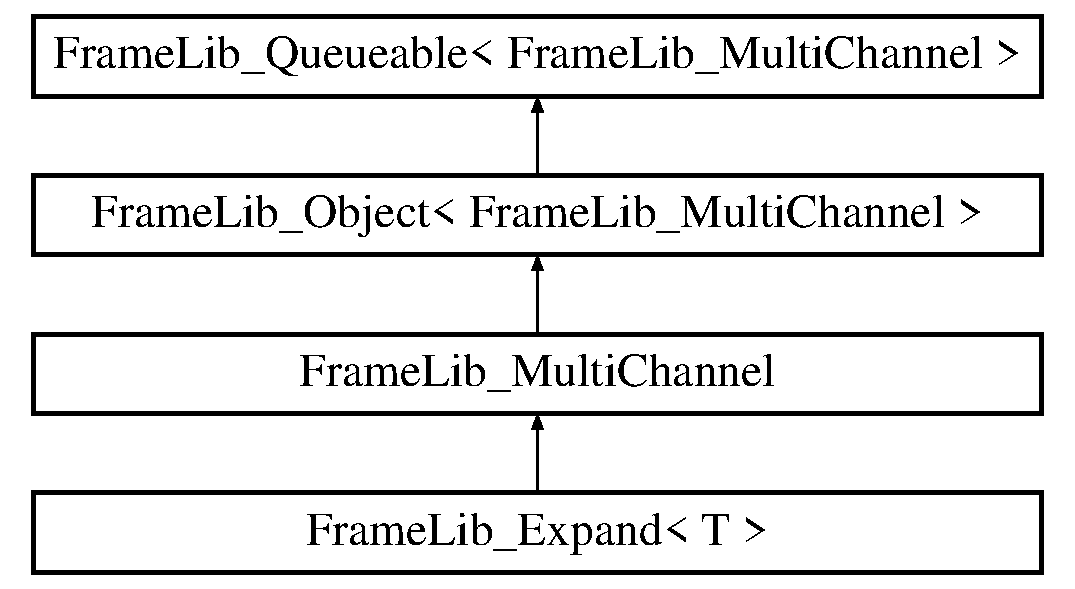
\includegraphics[height=4.000000cm]{class_frame_lib___expand}
\end{center}
\end{figure}
\subsection*{Public Member Functions}
\begin{DoxyCompactItemize}
\item 
\hyperlink{class_frame_lib___expand_a591240aee95c812856a9835b8014a915}{Frame\+Lib\+\_\+\+Expand} (\hyperlink{class_frame_lib___context}{Frame\+Lib\+\_\+\+Context} context, \hyperlink{class_frame_lib___parameters_1_1_serial}{Frame\+Lib\+\_\+\+Parameters\+::\+Serial} $\ast$serialised\+Parameters, void $\ast$owner)
\item 
\hyperlink{class_frame_lib___expand_a3aa2aa689e4b063fa65fe72be311c45f}{$\sim$\+Frame\+Lib\+\_\+\+Expand} ()
\item 
virtual void \hyperlink{class_frame_lib___expand_a73f7bf4264d45f56f249d6303b3e4c35}{set\+Fixed\+Input} (unsigned long idx, double $\ast$input, unsigned long size)
\item 
virtual void \hyperlink{class_frame_lib___expand_ae712d631cb99284e91c3f318534b3c03}{block\+Update} (double $\ast$$\ast$ins, double $\ast$$\ast$outs, unsigned long \hyperlink{_frame_lib___memory_8cpp_a8ef7d53a4cac28bf580a61f265fcaaa6}{block\+Size})
\item 
virtual void \hyperlink{class_frame_lib___expand_a579f16ec32e05ff84ee766038012fc3f}{reset} (double sampling\+Rate, unsigned long max\+Block\+Size)
\item 
virtual std\+::string \hyperlink{class_frame_lib___expand_ac4527eab2bfb55a38bd796d95f2a2562}{object\+Info} (bool verbose)
\item 
virtual std\+::string \hyperlink{class_frame_lib___expand_ab9017c7fe8562857609fcf819b7d1cdd}{input\+Info} (unsigned long idx, bool verbose)
\item 
virtual std\+::string \hyperlink{class_frame_lib___expand_abba12bed97c0b76095f1e1a699591b3e}{output\+Info} (unsigned long idx, bool verbose)
\item 
virtual std\+::string \hyperlink{class_frame_lib___expand_a94ab97ff114452551719fad428fd2d6e}{audio\+Info} (unsigned long idx, bool verbose)
\item 
virtual \hyperlink{_frame_lib___types_8h_ad495a9f61af7fff07d7e97979d1ab854}{Frame\+Type} \hyperlink{class_frame_lib___expand_abfe5f5550062e7cb351d45111dd2958c}{input\+Type} (unsigned long idx) const
\item 
virtual \hyperlink{_frame_lib___types_8h_ad495a9f61af7fff07d7e97979d1ab854}{Frame\+Type} \hyperlink{class_frame_lib___expand_a5ab23cdee5ca51ed5098b8a99164aa6a}{output\+Type} (unsigned long idx) const
\item 
virtual const \hyperlink{class_frame_lib___parameters}{Frame\+Lib\+\_\+\+Parameters} $\ast$ \hyperlink{class_frame_lib___expand_ae399eee75f1f0d854505eb67f8fb4dd0}{get\+Parameters} () const
\item 
virtual void \hyperlink{class_frame_lib___expand_ab3f908391944bd2d6f5492cc67c19cba}{auto\+Ordering\+Connections} ()
\item 
virtual void \hyperlink{class_frame_lib___expand_adbf3c1e77474e23eacabb395409424e5}{clear\+Auto\+Ordering\+Connections} ()
\end{DoxyCompactItemize}
\subsection*{Static Public Member Functions}
\begin{DoxyCompactItemize}
\item 
static bool \hyperlink{class_frame_lib___expand_a77c0e4af675ebb2ac3f47b26939ab94b}{handles\+Audio} ()
\end{DoxyCompactItemize}
\subsection*{Additional Inherited Members}


\subsection{Constructor \& Destructor Documentation}
\mbox{\Hypertarget{class_frame_lib___expand_a591240aee95c812856a9835b8014a915}\label{class_frame_lib___expand_a591240aee95c812856a9835b8014a915}} 
\index{Frame\+Lib\+\_\+\+Expand@{Frame\+Lib\+\_\+\+Expand}!Frame\+Lib\+\_\+\+Expand@{Frame\+Lib\+\_\+\+Expand}}
\index{Frame\+Lib\+\_\+\+Expand@{Frame\+Lib\+\_\+\+Expand}!Frame\+Lib\+\_\+\+Expand@{Frame\+Lib\+\_\+\+Expand}}
\subsubsection{\texorpdfstring{Frame\+Lib\+\_\+\+Expand()}{FrameLib\_Expand()}}
{\footnotesize\ttfamily template$<$class T $>$ \\
\hyperlink{class_frame_lib___expand}{Frame\+Lib\+\_\+\+Expand}$<$ T $>$\+::\hyperlink{class_frame_lib___expand}{Frame\+Lib\+\_\+\+Expand} (\begin{DoxyParamCaption}\item[{\hyperlink{class_frame_lib___context}{Frame\+Lib\+\_\+\+Context}}]{context,  }\item[{\hyperlink{class_frame_lib___parameters_1_1_serial}{Frame\+Lib\+\_\+\+Parameters\+::\+Serial} $\ast$}]{serialised\+Parameters,  }\item[{void $\ast$}]{owner }\end{DoxyParamCaption})\hspace{0.3cm}{\ttfamily [inline]}}

\mbox{\Hypertarget{class_frame_lib___expand_a3aa2aa689e4b063fa65fe72be311c45f}\label{class_frame_lib___expand_a3aa2aa689e4b063fa65fe72be311c45f}} 
\index{Frame\+Lib\+\_\+\+Expand@{Frame\+Lib\+\_\+\+Expand}!````~Frame\+Lib\+\_\+\+Expand@{$\sim$\+Frame\+Lib\+\_\+\+Expand}}
\index{````~Frame\+Lib\+\_\+\+Expand@{$\sim$\+Frame\+Lib\+\_\+\+Expand}!Frame\+Lib\+\_\+\+Expand@{Frame\+Lib\+\_\+\+Expand}}
\subsubsection{\texorpdfstring{$\sim$\+Frame\+Lib\+\_\+\+Expand()}{~FrameLib\_Expand()}}
{\footnotesize\ttfamily template$<$class T $>$ \\
\hyperlink{class_frame_lib___expand}{Frame\+Lib\+\_\+\+Expand}$<$ T $>$\+::$\sim$\hyperlink{class_frame_lib___expand}{Frame\+Lib\+\_\+\+Expand} (\begin{DoxyParamCaption}{ }\end{DoxyParamCaption})\hspace{0.3cm}{\ttfamily [inline]}}



\subsection{Member Function Documentation}
\mbox{\Hypertarget{class_frame_lib___expand_a94ab97ff114452551719fad428fd2d6e}\label{class_frame_lib___expand_a94ab97ff114452551719fad428fd2d6e}} 
\index{Frame\+Lib\+\_\+\+Expand@{Frame\+Lib\+\_\+\+Expand}!audio\+Info@{audio\+Info}}
\index{audio\+Info@{audio\+Info}!Frame\+Lib\+\_\+\+Expand@{Frame\+Lib\+\_\+\+Expand}}
\subsubsection{\texorpdfstring{audio\+Info()}{audioInfo()}}
{\footnotesize\ttfamily template$<$class T $>$ \\
virtual std\+::string \hyperlink{class_frame_lib___expand}{Frame\+Lib\+\_\+\+Expand}$<$ T $>$\+::audio\+Info (\begin{DoxyParamCaption}\item[{unsigned long}]{idx,  }\item[{bool}]{verbose }\end{DoxyParamCaption})\hspace{0.3cm}{\ttfamily [inline]}, {\ttfamily [virtual]}}



Reimplemented from \hyperlink{class_frame_lib___object_af618fcdec82b457911147c7c293bedd7}{Frame\+Lib\+\_\+\+Object$<$ Frame\+Lib\+\_\+\+Multi\+Channel $>$}.

\mbox{\Hypertarget{class_frame_lib___expand_ab3f908391944bd2d6f5492cc67c19cba}\label{class_frame_lib___expand_ab3f908391944bd2d6f5492cc67c19cba}} 
\index{Frame\+Lib\+\_\+\+Expand@{Frame\+Lib\+\_\+\+Expand}!auto\+Ordering\+Connections@{auto\+Ordering\+Connections}}
\index{auto\+Ordering\+Connections@{auto\+Ordering\+Connections}!Frame\+Lib\+\_\+\+Expand@{Frame\+Lib\+\_\+\+Expand}}
\subsubsection{\texorpdfstring{auto\+Ordering\+Connections()}{autoOrderingConnections()}}
{\footnotesize\ttfamily template$<$class T $>$ \\
virtual void \hyperlink{class_frame_lib___expand}{Frame\+Lib\+\_\+\+Expand}$<$ T $>$\+::auto\+Ordering\+Connections (\begin{DoxyParamCaption}{ }\end{DoxyParamCaption})\hspace{0.3cm}{\ttfamily [inline]}, {\ttfamily [virtual]}}



Implements \hyperlink{class_frame_lib___object_afa5bb93302a641c23b5eac7ab0dfe516}{Frame\+Lib\+\_\+\+Object$<$ Frame\+Lib\+\_\+\+Multi\+Channel $>$}.

\mbox{\Hypertarget{class_frame_lib___expand_ae712d631cb99284e91c3f318534b3c03}\label{class_frame_lib___expand_ae712d631cb99284e91c3f318534b3c03}} 
\index{Frame\+Lib\+\_\+\+Expand@{Frame\+Lib\+\_\+\+Expand}!block\+Update@{block\+Update}}
\index{block\+Update@{block\+Update}!Frame\+Lib\+\_\+\+Expand@{Frame\+Lib\+\_\+\+Expand}}
\subsubsection{\texorpdfstring{block\+Update()}{blockUpdate()}}
{\footnotesize\ttfamily template$<$class T $>$ \\
virtual void \hyperlink{class_frame_lib___expand}{Frame\+Lib\+\_\+\+Expand}$<$ T $>$\+::block\+Update (\begin{DoxyParamCaption}\item[{double $\ast$$\ast$}]{ins,  }\item[{double $\ast$$\ast$}]{outs,  }\item[{unsigned long}]{block\+Size }\end{DoxyParamCaption})\hspace{0.3cm}{\ttfamily [inline]}, {\ttfamily [virtual]}}



Reimplemented from \hyperlink{class_frame_lib___multi_channel_a8ad8f1c0138f32ef0bfb7e4673b34d30}{Frame\+Lib\+\_\+\+Multi\+Channel}.

\mbox{\Hypertarget{class_frame_lib___expand_adbf3c1e77474e23eacabb395409424e5}\label{class_frame_lib___expand_adbf3c1e77474e23eacabb395409424e5}} 
\index{Frame\+Lib\+\_\+\+Expand@{Frame\+Lib\+\_\+\+Expand}!clear\+Auto\+Ordering\+Connections@{clear\+Auto\+Ordering\+Connections}}
\index{clear\+Auto\+Ordering\+Connections@{clear\+Auto\+Ordering\+Connections}!Frame\+Lib\+\_\+\+Expand@{Frame\+Lib\+\_\+\+Expand}}
\subsubsection{\texorpdfstring{clear\+Auto\+Ordering\+Connections()}{clearAutoOrderingConnections()}}
{\footnotesize\ttfamily template$<$class T $>$ \\
virtual void \hyperlink{class_frame_lib___expand}{Frame\+Lib\+\_\+\+Expand}$<$ T $>$\+::clear\+Auto\+Ordering\+Connections (\begin{DoxyParamCaption}{ }\end{DoxyParamCaption})\hspace{0.3cm}{\ttfamily [inline]}, {\ttfamily [virtual]}}



Implements \hyperlink{class_frame_lib___object_aac43ebfacb59081f7f60957380df7481}{Frame\+Lib\+\_\+\+Object$<$ Frame\+Lib\+\_\+\+Multi\+Channel $>$}.

\mbox{\Hypertarget{class_frame_lib___expand_ae399eee75f1f0d854505eb67f8fb4dd0}\label{class_frame_lib___expand_ae399eee75f1f0d854505eb67f8fb4dd0}} 
\index{Frame\+Lib\+\_\+\+Expand@{Frame\+Lib\+\_\+\+Expand}!get\+Parameters@{get\+Parameters}}
\index{get\+Parameters@{get\+Parameters}!Frame\+Lib\+\_\+\+Expand@{Frame\+Lib\+\_\+\+Expand}}
\subsubsection{\texorpdfstring{get\+Parameters()}{getParameters()}}
{\footnotesize\ttfamily template$<$class T $>$ \\
virtual const \hyperlink{class_frame_lib___parameters}{Frame\+Lib\+\_\+\+Parameters}$\ast$ \hyperlink{class_frame_lib___expand}{Frame\+Lib\+\_\+\+Expand}$<$ T $>$\+::get\+Parameters (\begin{DoxyParamCaption}{ }\end{DoxyParamCaption}) const\hspace{0.3cm}{\ttfamily [inline]}, {\ttfamily [virtual]}}



Reimplemented from \hyperlink{class_frame_lib___object_ac90a6770aeef26ee1601889dc16dba56}{Frame\+Lib\+\_\+\+Object$<$ Frame\+Lib\+\_\+\+Multi\+Channel $>$}.

\mbox{\Hypertarget{class_frame_lib___expand_a77c0e4af675ebb2ac3f47b26939ab94b}\label{class_frame_lib___expand_a77c0e4af675ebb2ac3f47b26939ab94b}} 
\index{Frame\+Lib\+\_\+\+Expand@{Frame\+Lib\+\_\+\+Expand}!handles\+Audio@{handles\+Audio}}
\index{handles\+Audio@{handles\+Audio}!Frame\+Lib\+\_\+\+Expand@{Frame\+Lib\+\_\+\+Expand}}
\subsubsection{\texorpdfstring{handles\+Audio()}{handlesAudio()}}
{\footnotesize\ttfamily template$<$class T $>$ \\
static bool \hyperlink{class_frame_lib___expand}{Frame\+Lib\+\_\+\+Expand}$<$ T $>$\+::handles\+Audio (\begin{DoxyParamCaption}{ }\end{DoxyParamCaption})\hspace{0.3cm}{\ttfamily [inline]}, {\ttfamily [static]}}

\mbox{\Hypertarget{class_frame_lib___expand_ab9017c7fe8562857609fcf819b7d1cdd}\label{class_frame_lib___expand_ab9017c7fe8562857609fcf819b7d1cdd}} 
\index{Frame\+Lib\+\_\+\+Expand@{Frame\+Lib\+\_\+\+Expand}!input\+Info@{input\+Info}}
\index{input\+Info@{input\+Info}!Frame\+Lib\+\_\+\+Expand@{Frame\+Lib\+\_\+\+Expand}}
\subsubsection{\texorpdfstring{input\+Info()}{inputInfo()}}
{\footnotesize\ttfamily template$<$class T $>$ \\
virtual std\+::string \hyperlink{class_frame_lib___expand}{Frame\+Lib\+\_\+\+Expand}$<$ T $>$\+::input\+Info (\begin{DoxyParamCaption}\item[{unsigned long}]{idx,  }\item[{bool}]{verbose }\end{DoxyParamCaption})\hspace{0.3cm}{\ttfamily [inline]}, {\ttfamily [virtual]}}



Reimplemented from \hyperlink{class_frame_lib___object_a49abea5f18125c425b1eae8710735891}{Frame\+Lib\+\_\+\+Object$<$ Frame\+Lib\+\_\+\+Multi\+Channel $>$}.

\mbox{\Hypertarget{class_frame_lib___expand_abfe5f5550062e7cb351d45111dd2958c}\label{class_frame_lib___expand_abfe5f5550062e7cb351d45111dd2958c}} 
\index{Frame\+Lib\+\_\+\+Expand@{Frame\+Lib\+\_\+\+Expand}!input\+Type@{input\+Type}}
\index{input\+Type@{input\+Type}!Frame\+Lib\+\_\+\+Expand@{Frame\+Lib\+\_\+\+Expand}}
\subsubsection{\texorpdfstring{input\+Type()}{inputType()}}
{\footnotesize\ttfamily template$<$class T $>$ \\
virtual \hyperlink{_frame_lib___types_8h_ad495a9f61af7fff07d7e97979d1ab854}{Frame\+Type} \hyperlink{class_frame_lib___expand}{Frame\+Lib\+\_\+\+Expand}$<$ T $>$\+::input\+Type (\begin{DoxyParamCaption}\item[{unsigned long}]{idx }\end{DoxyParamCaption}) const\hspace{0.3cm}{\ttfamily [inline]}, {\ttfamily [virtual]}}



Implements \hyperlink{class_frame_lib___object_ab1ab1ae8180bb8b7e881aac6a4e1066c}{Frame\+Lib\+\_\+\+Object$<$ Frame\+Lib\+\_\+\+Multi\+Channel $>$}.

\mbox{\Hypertarget{class_frame_lib___expand_ac4527eab2bfb55a38bd796d95f2a2562}\label{class_frame_lib___expand_ac4527eab2bfb55a38bd796d95f2a2562}} 
\index{Frame\+Lib\+\_\+\+Expand@{Frame\+Lib\+\_\+\+Expand}!object\+Info@{object\+Info}}
\index{object\+Info@{object\+Info}!Frame\+Lib\+\_\+\+Expand@{Frame\+Lib\+\_\+\+Expand}}
\subsubsection{\texorpdfstring{object\+Info()}{objectInfo()}}
{\footnotesize\ttfamily template$<$class T $>$ \\
virtual std\+::string \hyperlink{class_frame_lib___expand}{Frame\+Lib\+\_\+\+Expand}$<$ T $>$\+::object\+Info (\begin{DoxyParamCaption}\item[{bool}]{verbose }\end{DoxyParamCaption})\hspace{0.3cm}{\ttfamily [inline]}, {\ttfamily [virtual]}}



Reimplemented from \hyperlink{class_frame_lib___object_a10d673de9a3c59ace6a22ba1cff313c8}{Frame\+Lib\+\_\+\+Object$<$ Frame\+Lib\+\_\+\+Multi\+Channel $>$}.

\mbox{\Hypertarget{class_frame_lib___expand_abba12bed97c0b76095f1e1a699591b3e}\label{class_frame_lib___expand_abba12bed97c0b76095f1e1a699591b3e}} 
\index{Frame\+Lib\+\_\+\+Expand@{Frame\+Lib\+\_\+\+Expand}!output\+Info@{output\+Info}}
\index{output\+Info@{output\+Info}!Frame\+Lib\+\_\+\+Expand@{Frame\+Lib\+\_\+\+Expand}}
\subsubsection{\texorpdfstring{output\+Info()}{outputInfo()}}
{\footnotesize\ttfamily template$<$class T $>$ \\
virtual std\+::string \hyperlink{class_frame_lib___expand}{Frame\+Lib\+\_\+\+Expand}$<$ T $>$\+::output\+Info (\begin{DoxyParamCaption}\item[{unsigned long}]{idx,  }\item[{bool}]{verbose }\end{DoxyParamCaption})\hspace{0.3cm}{\ttfamily [inline]}, {\ttfamily [virtual]}}



Reimplemented from \hyperlink{class_frame_lib___object_a6e6d79e8d620eedbaa50abf324cdedf5}{Frame\+Lib\+\_\+\+Object$<$ Frame\+Lib\+\_\+\+Multi\+Channel $>$}.

\mbox{\Hypertarget{class_frame_lib___expand_a5ab23cdee5ca51ed5098b8a99164aa6a}\label{class_frame_lib___expand_a5ab23cdee5ca51ed5098b8a99164aa6a}} 
\index{Frame\+Lib\+\_\+\+Expand@{Frame\+Lib\+\_\+\+Expand}!output\+Type@{output\+Type}}
\index{output\+Type@{output\+Type}!Frame\+Lib\+\_\+\+Expand@{Frame\+Lib\+\_\+\+Expand}}
\subsubsection{\texorpdfstring{output\+Type()}{outputType()}}
{\footnotesize\ttfamily template$<$class T $>$ \\
virtual \hyperlink{_frame_lib___types_8h_ad495a9f61af7fff07d7e97979d1ab854}{Frame\+Type} \hyperlink{class_frame_lib___expand}{Frame\+Lib\+\_\+\+Expand}$<$ T $>$\+::output\+Type (\begin{DoxyParamCaption}\item[{unsigned long}]{idx }\end{DoxyParamCaption}) const\hspace{0.3cm}{\ttfamily [inline]}, {\ttfamily [virtual]}}



Implements \hyperlink{class_frame_lib___object_a03eb408844f15d8f73cee67f43149b9d}{Frame\+Lib\+\_\+\+Object$<$ Frame\+Lib\+\_\+\+Multi\+Channel $>$}.

\mbox{\Hypertarget{class_frame_lib___expand_a579f16ec32e05ff84ee766038012fc3f}\label{class_frame_lib___expand_a579f16ec32e05ff84ee766038012fc3f}} 
\index{Frame\+Lib\+\_\+\+Expand@{Frame\+Lib\+\_\+\+Expand}!reset@{reset}}
\index{reset@{reset}!Frame\+Lib\+\_\+\+Expand@{Frame\+Lib\+\_\+\+Expand}}
\subsubsection{\texorpdfstring{reset()}{reset()}}
{\footnotesize\ttfamily template$<$class T $>$ \\
virtual void \hyperlink{class_frame_lib___expand}{Frame\+Lib\+\_\+\+Expand}$<$ T $>$\+::reset (\begin{DoxyParamCaption}\item[{double}]{sampling\+Rate,  }\item[{unsigned long}]{max\+Block\+Size }\end{DoxyParamCaption})\hspace{0.3cm}{\ttfamily [inline]}, {\ttfamily [virtual]}}



Reimplemented from \hyperlink{class_frame_lib___multi_channel_af27f3dca507c48459452be825b4c0c72}{Frame\+Lib\+\_\+\+Multi\+Channel}.

\mbox{\Hypertarget{class_frame_lib___expand_a73f7bf4264d45f56f249d6303b3e4c35}\label{class_frame_lib___expand_a73f7bf4264d45f56f249d6303b3e4c35}} 
\index{Frame\+Lib\+\_\+\+Expand@{Frame\+Lib\+\_\+\+Expand}!set\+Fixed\+Input@{set\+Fixed\+Input}}
\index{set\+Fixed\+Input@{set\+Fixed\+Input}!Frame\+Lib\+\_\+\+Expand@{Frame\+Lib\+\_\+\+Expand}}
\subsubsection{\texorpdfstring{set\+Fixed\+Input()}{setFixedInput()}}
{\footnotesize\ttfamily template$<$class T $>$ \\
virtual void \hyperlink{class_frame_lib___expand}{Frame\+Lib\+\_\+\+Expand}$<$ T $>$\+::set\+Fixed\+Input (\begin{DoxyParamCaption}\item[{unsigned long}]{idx,  }\item[{double $\ast$}]{input,  }\item[{unsigned long}]{size }\end{DoxyParamCaption})\hspace{0.3cm}{\ttfamily [inline]}, {\ttfamily [virtual]}}



Reimplemented from \hyperlink{class_frame_lib___multi_channel_a2bbd1050ff53556bf671282312857301}{Frame\+Lib\+\_\+\+Multi\+Channel}.



The documentation for this class was generated from the following file\+:\begin{DoxyCompactItemize}
\item 
/\+Users/alexharker/\+Documents/\+Max Externals/\+Frame\+Lib/\+Frame\+Lib\+\_\+\+Framework/\hyperlink{_frame_lib___multichannel_8h}{Frame\+Lib\+\_\+\+Multichannel.\+h}\end{DoxyCompactItemize}

\hypertarget{class_frame_lib___global}{}\section{Frame\+Lib\+\_\+\+Global Class Reference}
\label{class_frame_lib___global}\index{Frame\+Lib\+\_\+\+Global@{Frame\+Lib\+\_\+\+Global}}


{\ttfamily \#include $<$Frame\+Lib\+\_\+\+Global.\+h$>$}

\subsection*{Public Member Functions}
\begin{DoxyCompactItemize}
\item 
\hyperlink{class_frame_lib___local_allocator}{Frame\+Lib\+\_\+\+Local\+Allocator} $\ast$ \hyperlink{class_frame_lib___global_a31c3fae37e27c9cce286d30ed30838d3}{get\+Allocator} (void $\ast$reference)
\item 
\hyperlink{class_frame_lib___connection_queue}{Frame\+Lib\+\_\+\+Connection\+Queue} $\ast$ \hyperlink{class_frame_lib___global_ae0cfe1ff49ba163758fcb66f9e94b991}{get\+Connection\+Queue} (void $\ast$reference)
\item 
\hyperlink{class_frame_lib___d_s_p_queue}{Frame\+Lib\+\_\+\+D\+S\+P\+Queue} $\ast$ \hyperlink{class_frame_lib___global_a5b4e45a675ea406538781011f7ebc153}{get\+D\+S\+P\+Queue} (void $\ast$reference)
\item 
void \hyperlink{class_frame_lib___global_a78b0ff45eb662f12c41bdd641a416539}{release\+Allocator} (void $\ast$reference)
\item 
void \hyperlink{class_frame_lib___global_ab461ad3b4bdd9c580018373cf1617b1b}{release\+Connection\+Queue} (void $\ast$reference)
\item 
void \hyperlink{class_frame_lib___global_a118b451294a2893fa60edfb09f60002a}{release\+D\+S\+P\+Queue} (void $\ast$reference)
\end{DoxyCompactItemize}
\subsection*{Static Public Member Functions}
\begin{DoxyCompactItemize}
\item 
static \hyperlink{class_frame_lib___global}{Frame\+Lib\+\_\+\+Global} $\ast$ \hyperlink{class_frame_lib___global_ac9a895677da386e8fde525c061a854e4}{get} (\hyperlink{class_frame_lib___global}{Frame\+Lib\+\_\+\+Global} $\ast$$\ast$global)
\item 
static void \hyperlink{class_frame_lib___global_a079e2b866b66d477ae551e0b0e12ea11}{release} (\hyperlink{class_frame_lib___global}{Frame\+Lib\+\_\+\+Global} $\ast$$\ast$global)
\end{DoxyCompactItemize}


\subsection{Member Function Documentation}
\mbox{\Hypertarget{class_frame_lib___global_ac9a895677da386e8fde525c061a854e4}\label{class_frame_lib___global_ac9a895677da386e8fde525c061a854e4}} 
\index{Frame\+Lib\+\_\+\+Global@{Frame\+Lib\+\_\+\+Global}!get@{get}}
\index{get@{get}!Frame\+Lib\+\_\+\+Global@{Frame\+Lib\+\_\+\+Global}}
\subsubsection{\texorpdfstring{get()}{get()}}
{\footnotesize\ttfamily \hyperlink{class_frame_lib___global}{Frame\+Lib\+\_\+\+Global} $\ast$ Frame\+Lib\+\_\+\+Global\+::get (\begin{DoxyParamCaption}\item[{\hyperlink{class_frame_lib___global}{Frame\+Lib\+\_\+\+Global} $\ast$$\ast$}]{global }\end{DoxyParamCaption})\hspace{0.3cm}{\ttfamily [static]}}

\mbox{\Hypertarget{class_frame_lib___global_a31c3fae37e27c9cce286d30ed30838d3}\label{class_frame_lib___global_a31c3fae37e27c9cce286d30ed30838d3}} 
\index{Frame\+Lib\+\_\+\+Global@{Frame\+Lib\+\_\+\+Global}!get\+Allocator@{get\+Allocator}}
\index{get\+Allocator@{get\+Allocator}!Frame\+Lib\+\_\+\+Global@{Frame\+Lib\+\_\+\+Global}}
\subsubsection{\texorpdfstring{get\+Allocator()}{getAllocator()}}
{\footnotesize\ttfamily \hyperlink{class_frame_lib___local_allocator}{Frame\+Lib\+\_\+\+Local\+Allocator} $\ast$ Frame\+Lib\+\_\+\+Global\+::get\+Allocator (\begin{DoxyParamCaption}\item[{void $\ast$}]{reference }\end{DoxyParamCaption})}

\mbox{\Hypertarget{class_frame_lib___global_ae0cfe1ff49ba163758fcb66f9e94b991}\label{class_frame_lib___global_ae0cfe1ff49ba163758fcb66f9e94b991}} 
\index{Frame\+Lib\+\_\+\+Global@{Frame\+Lib\+\_\+\+Global}!get\+Connection\+Queue@{get\+Connection\+Queue}}
\index{get\+Connection\+Queue@{get\+Connection\+Queue}!Frame\+Lib\+\_\+\+Global@{Frame\+Lib\+\_\+\+Global}}
\subsubsection{\texorpdfstring{get\+Connection\+Queue()}{getConnectionQueue()}}
{\footnotesize\ttfamily \hyperlink{class_frame_lib___connection_queue}{Frame\+Lib\+\_\+\+Connection\+Queue} $\ast$ Frame\+Lib\+\_\+\+Global\+::get\+Connection\+Queue (\begin{DoxyParamCaption}\item[{void $\ast$}]{reference }\end{DoxyParamCaption})}

\mbox{\Hypertarget{class_frame_lib___global_a5b4e45a675ea406538781011f7ebc153}\label{class_frame_lib___global_a5b4e45a675ea406538781011f7ebc153}} 
\index{Frame\+Lib\+\_\+\+Global@{Frame\+Lib\+\_\+\+Global}!get\+D\+S\+P\+Queue@{get\+D\+S\+P\+Queue}}
\index{get\+D\+S\+P\+Queue@{get\+D\+S\+P\+Queue}!Frame\+Lib\+\_\+\+Global@{Frame\+Lib\+\_\+\+Global}}
\subsubsection{\texorpdfstring{get\+D\+S\+P\+Queue()}{getDSPQueue()}}
{\footnotesize\ttfamily \hyperlink{class_frame_lib___d_s_p_queue}{Frame\+Lib\+\_\+\+D\+S\+P\+Queue} $\ast$ Frame\+Lib\+\_\+\+Global\+::get\+D\+S\+P\+Queue (\begin{DoxyParamCaption}\item[{void $\ast$}]{reference }\end{DoxyParamCaption})}

\mbox{\Hypertarget{class_frame_lib___global_a079e2b866b66d477ae551e0b0e12ea11}\label{class_frame_lib___global_a079e2b866b66d477ae551e0b0e12ea11}} 
\index{Frame\+Lib\+\_\+\+Global@{Frame\+Lib\+\_\+\+Global}!release@{release}}
\index{release@{release}!Frame\+Lib\+\_\+\+Global@{Frame\+Lib\+\_\+\+Global}}
\subsubsection{\texorpdfstring{release()}{release()}}
{\footnotesize\ttfamily void Frame\+Lib\+\_\+\+Global\+::release (\begin{DoxyParamCaption}\item[{\hyperlink{class_frame_lib___global}{Frame\+Lib\+\_\+\+Global} $\ast$$\ast$}]{global }\end{DoxyParamCaption})\hspace{0.3cm}{\ttfamily [static]}}

\mbox{\Hypertarget{class_frame_lib___global_a78b0ff45eb662f12c41bdd641a416539}\label{class_frame_lib___global_a78b0ff45eb662f12c41bdd641a416539}} 
\index{Frame\+Lib\+\_\+\+Global@{Frame\+Lib\+\_\+\+Global}!release\+Allocator@{release\+Allocator}}
\index{release\+Allocator@{release\+Allocator}!Frame\+Lib\+\_\+\+Global@{Frame\+Lib\+\_\+\+Global}}
\subsubsection{\texorpdfstring{release\+Allocator()}{releaseAllocator()}}
{\footnotesize\ttfamily void Frame\+Lib\+\_\+\+Global\+::release\+Allocator (\begin{DoxyParamCaption}\item[{void $\ast$}]{reference }\end{DoxyParamCaption})}

\mbox{\Hypertarget{class_frame_lib___global_ab461ad3b4bdd9c580018373cf1617b1b}\label{class_frame_lib___global_ab461ad3b4bdd9c580018373cf1617b1b}} 
\index{Frame\+Lib\+\_\+\+Global@{Frame\+Lib\+\_\+\+Global}!release\+Connection\+Queue@{release\+Connection\+Queue}}
\index{release\+Connection\+Queue@{release\+Connection\+Queue}!Frame\+Lib\+\_\+\+Global@{Frame\+Lib\+\_\+\+Global}}
\subsubsection{\texorpdfstring{release\+Connection\+Queue()}{releaseConnectionQueue()}}
{\footnotesize\ttfamily void Frame\+Lib\+\_\+\+Global\+::release\+Connection\+Queue (\begin{DoxyParamCaption}\item[{void $\ast$}]{reference }\end{DoxyParamCaption})}

\mbox{\Hypertarget{class_frame_lib___global_a118b451294a2893fa60edfb09f60002a}\label{class_frame_lib___global_a118b451294a2893fa60edfb09f60002a}} 
\index{Frame\+Lib\+\_\+\+Global@{Frame\+Lib\+\_\+\+Global}!release\+D\+S\+P\+Queue@{release\+D\+S\+P\+Queue}}
\index{release\+D\+S\+P\+Queue@{release\+D\+S\+P\+Queue}!Frame\+Lib\+\_\+\+Global@{Frame\+Lib\+\_\+\+Global}}
\subsubsection{\texorpdfstring{release\+D\+S\+P\+Queue()}{releaseDSPQueue()}}
{\footnotesize\ttfamily void Frame\+Lib\+\_\+\+Global\+::release\+D\+S\+P\+Queue (\begin{DoxyParamCaption}\item[{void $\ast$}]{reference }\end{DoxyParamCaption})}



The documentation for this class was generated from the following files\+:\begin{DoxyCompactItemize}
\item 
Frame\+Lib\+\_\+\+Framework/\hyperlink{_frame_lib___global_8h}{Frame\+Lib\+\_\+\+Global.\+h}\item 
Frame\+Lib\+\_\+\+Framework/\hyperlink{_frame_lib___global_8cpp}{Frame\+Lib\+\_\+\+Global.\+cpp}\end{DoxyCompactItemize}

\hypertarget{class_frame_lib___global_allocator}{}\section{Frame\+Lib\+\_\+\+Global\+Allocator Class Reference}
\label{class_frame_lib___global_allocator}\index{Frame\+Lib\+\_\+\+Global\+Allocator@{Frame\+Lib\+\_\+\+Global\+Allocator}}


a global threadsafe memory allocator suitable for realtime usage.  




{\ttfamily \#include $<$Frame\+Lib\+\_\+\+Memory.\+h$>$}

\subsection*{Classes}
\begin{DoxyCompactItemize}
\item 
class \hyperlink{class_frame_lib___global_allocator_1_1_pruner}{Pruner}
\begin{DoxyCompactList}\small\item\em an R\+A\+II utility for repeated deallocation with only a single lock. \end{DoxyCompactList}\end{DoxyCompactItemize}
\subsection*{Public Member Functions}
\begin{DoxyCompactItemize}
\item 
\hyperlink{class_frame_lib___global_allocator_aeb0d7259cd6bb4c5b8e365a26e370e54}{Frame\+Lib\+\_\+\+Global\+Allocator} (\hyperlink{class_frame_lib___error_reporter}{Frame\+Lib\+\_\+\+Error\+Reporter} \&error\+Reporter)
\item 
\hyperlink{class_frame_lib___global_allocator_a20fa9b3b84bb54eefffb8f30a70883d5}{$\sim$\+Frame\+Lib\+\_\+\+Global\+Allocator} ()
\item 
\hyperlink{class_frame_lib___global_allocator_a7e93abd711eb6acf04601aef3c6b9877}{Frame\+Lib\+\_\+\+Global\+Allocator} (const \hyperlink{class_frame_lib___global_allocator}{Frame\+Lib\+\_\+\+Global\+Allocator} \&)=delete
\item 
\hyperlink{class_frame_lib___global_allocator}{Frame\+Lib\+\_\+\+Global\+Allocator} \& \hyperlink{class_frame_lib___global_allocator_a23d4689821a194c5f89227d135a5703c}{operator=} (const \hyperlink{class_frame_lib___global_allocator}{Frame\+Lib\+\_\+\+Global\+Allocator} \&)=delete
\item 
void $\ast$ \hyperlink{class_frame_lib___global_allocator_af2ef32b9cba8f46c836be2d1df31d8a4}{alloc} (size\+\_\+t size)
\item 
void \hyperlink{class_frame_lib___global_allocator_a8cd36632acf1f6f281f50337bb95e2be}{dealloc} (void $\ast$ptr)
\end{DoxyCompactItemize}
\subsection*{Static Public Member Functions}
\begin{DoxyCompactItemize}
\item 
static size\+\_\+t \hyperlink{class_frame_lib___global_allocator_aebae4f9f17b2d460f7d27e2a68eb9ae8}{get\+Alignment} ()
\item 
static size\+\_\+t \hyperlink{class_frame_lib___global_allocator_a5568abfa871845e293c76e76a891b2ef}{align\+Size} (size\+\_\+t x)
\end{DoxyCompactItemize}


\subsection{Detailed Description}
a global threadsafe memory allocator suitable for realtime usage. 

\subsection{Constructor \& Destructor Documentation}
\mbox{\Hypertarget{class_frame_lib___global_allocator_aeb0d7259cd6bb4c5b8e365a26e370e54}\label{class_frame_lib___global_allocator_aeb0d7259cd6bb4c5b8e365a26e370e54}} 
\index{Frame\+Lib\+\_\+\+Global\+Allocator@{Frame\+Lib\+\_\+\+Global\+Allocator}!Frame\+Lib\+\_\+\+Global\+Allocator@{Frame\+Lib\+\_\+\+Global\+Allocator}}
\index{Frame\+Lib\+\_\+\+Global\+Allocator@{Frame\+Lib\+\_\+\+Global\+Allocator}!Frame\+Lib\+\_\+\+Global\+Allocator@{Frame\+Lib\+\_\+\+Global\+Allocator}}
\subsubsection{\texorpdfstring{Frame\+Lib\+\_\+\+Global\+Allocator()}{FrameLib\_GlobalAllocator()}\hspace{0.1cm}{\footnotesize\ttfamily [1/2]}}
{\footnotesize\ttfamily Frame\+Lib\+\_\+\+Global\+Allocator\+::\+Frame\+Lib\+\_\+\+Global\+Allocator (\begin{DoxyParamCaption}\item[{\hyperlink{class_frame_lib___error_reporter}{Frame\+Lib\+\_\+\+Error\+Reporter} \&}]{error\+Reporter }\end{DoxyParamCaption})\hspace{0.3cm}{\ttfamily [inline]}}

\mbox{\Hypertarget{class_frame_lib___global_allocator_a20fa9b3b84bb54eefffb8f30a70883d5}\label{class_frame_lib___global_allocator_a20fa9b3b84bb54eefffb8f30a70883d5}} 
\index{Frame\+Lib\+\_\+\+Global\+Allocator@{Frame\+Lib\+\_\+\+Global\+Allocator}!````~Frame\+Lib\+\_\+\+Global\+Allocator@{$\sim$\+Frame\+Lib\+\_\+\+Global\+Allocator}}
\index{````~Frame\+Lib\+\_\+\+Global\+Allocator@{$\sim$\+Frame\+Lib\+\_\+\+Global\+Allocator}!Frame\+Lib\+\_\+\+Global\+Allocator@{Frame\+Lib\+\_\+\+Global\+Allocator}}
\subsubsection{\texorpdfstring{$\sim$\+Frame\+Lib\+\_\+\+Global\+Allocator()}{~FrameLib\_GlobalAllocator()}}
{\footnotesize\ttfamily Frame\+Lib\+\_\+\+Global\+Allocator\+::$\sim$\+Frame\+Lib\+\_\+\+Global\+Allocator (\begin{DoxyParamCaption}{ }\end{DoxyParamCaption})\hspace{0.3cm}{\ttfamily [inline]}}

\mbox{\Hypertarget{class_frame_lib___global_allocator_a7e93abd711eb6acf04601aef3c6b9877}\label{class_frame_lib___global_allocator_a7e93abd711eb6acf04601aef3c6b9877}} 
\index{Frame\+Lib\+\_\+\+Global\+Allocator@{Frame\+Lib\+\_\+\+Global\+Allocator}!Frame\+Lib\+\_\+\+Global\+Allocator@{Frame\+Lib\+\_\+\+Global\+Allocator}}
\index{Frame\+Lib\+\_\+\+Global\+Allocator@{Frame\+Lib\+\_\+\+Global\+Allocator}!Frame\+Lib\+\_\+\+Global\+Allocator@{Frame\+Lib\+\_\+\+Global\+Allocator}}
\subsubsection{\texorpdfstring{Frame\+Lib\+\_\+\+Global\+Allocator()}{FrameLib\_GlobalAllocator()}\hspace{0.1cm}{\footnotesize\ttfamily [2/2]}}
{\footnotesize\ttfamily Frame\+Lib\+\_\+\+Global\+Allocator\+::\+Frame\+Lib\+\_\+\+Global\+Allocator (\begin{DoxyParamCaption}\item[{const \hyperlink{class_frame_lib___global_allocator}{Frame\+Lib\+\_\+\+Global\+Allocator} \&}]{ }\end{DoxyParamCaption})\hspace{0.3cm}{\ttfamily [delete]}}



\subsection{Member Function Documentation}
\mbox{\Hypertarget{class_frame_lib___global_allocator_a5568abfa871845e293c76e76a891b2ef}\label{class_frame_lib___global_allocator_a5568abfa871845e293c76e76a891b2ef}} 
\index{Frame\+Lib\+\_\+\+Global\+Allocator@{Frame\+Lib\+\_\+\+Global\+Allocator}!align\+Size@{align\+Size}}
\index{align\+Size@{align\+Size}!Frame\+Lib\+\_\+\+Global\+Allocator@{Frame\+Lib\+\_\+\+Global\+Allocator}}
\subsubsection{\texorpdfstring{align\+Size()}{alignSize()}}
{\footnotesize\ttfamily size\+\_\+t Frame\+Lib\+\_\+\+Global\+Allocator\+::align\+Size (\begin{DoxyParamCaption}\item[{size\+\_\+t}]{x }\end{DoxyParamCaption})\hspace{0.3cm}{\ttfamily [static]}}

\mbox{\Hypertarget{class_frame_lib___global_allocator_af2ef32b9cba8f46c836be2d1df31d8a4}\label{class_frame_lib___global_allocator_af2ef32b9cba8f46c836be2d1df31d8a4}} 
\index{Frame\+Lib\+\_\+\+Global\+Allocator@{Frame\+Lib\+\_\+\+Global\+Allocator}!alloc@{alloc}}
\index{alloc@{alloc}!Frame\+Lib\+\_\+\+Global\+Allocator@{Frame\+Lib\+\_\+\+Global\+Allocator}}
\subsubsection{\texorpdfstring{alloc()}{alloc()}}
{\footnotesize\ttfamily void $\ast$ Frame\+Lib\+\_\+\+Global\+Allocator\+::alloc (\begin{DoxyParamCaption}\item[{size\+\_\+t}]{size }\end{DoxyParamCaption})}

\mbox{\Hypertarget{class_frame_lib___global_allocator_a8cd36632acf1f6f281f50337bb95e2be}\label{class_frame_lib___global_allocator_a8cd36632acf1f6f281f50337bb95e2be}} 
\index{Frame\+Lib\+\_\+\+Global\+Allocator@{Frame\+Lib\+\_\+\+Global\+Allocator}!dealloc@{dealloc}}
\index{dealloc@{dealloc}!Frame\+Lib\+\_\+\+Global\+Allocator@{Frame\+Lib\+\_\+\+Global\+Allocator}}
\subsubsection{\texorpdfstring{dealloc()}{dealloc()}}
{\footnotesize\ttfamily void Frame\+Lib\+\_\+\+Global\+Allocator\+::dealloc (\begin{DoxyParamCaption}\item[{void $\ast$}]{ptr }\end{DoxyParamCaption})}

\mbox{\Hypertarget{class_frame_lib___global_allocator_aebae4f9f17b2d460f7d27e2a68eb9ae8}\label{class_frame_lib___global_allocator_aebae4f9f17b2d460f7d27e2a68eb9ae8}} 
\index{Frame\+Lib\+\_\+\+Global\+Allocator@{Frame\+Lib\+\_\+\+Global\+Allocator}!get\+Alignment@{get\+Alignment}}
\index{get\+Alignment@{get\+Alignment}!Frame\+Lib\+\_\+\+Global\+Allocator@{Frame\+Lib\+\_\+\+Global\+Allocator}}
\subsubsection{\texorpdfstring{get\+Alignment()}{getAlignment()}}
{\footnotesize\ttfamily size\+\_\+t Frame\+Lib\+\_\+\+Global\+Allocator\+::get\+Alignment (\begin{DoxyParamCaption}{ }\end{DoxyParamCaption})\hspace{0.3cm}{\ttfamily [static]}}

\mbox{\Hypertarget{class_frame_lib___global_allocator_a23d4689821a194c5f89227d135a5703c}\label{class_frame_lib___global_allocator_a23d4689821a194c5f89227d135a5703c}} 
\index{Frame\+Lib\+\_\+\+Global\+Allocator@{Frame\+Lib\+\_\+\+Global\+Allocator}!operator=@{operator=}}
\index{operator=@{operator=}!Frame\+Lib\+\_\+\+Global\+Allocator@{Frame\+Lib\+\_\+\+Global\+Allocator}}
\subsubsection{\texorpdfstring{operator=()}{operator=()}}
{\footnotesize\ttfamily \hyperlink{class_frame_lib___global_allocator}{Frame\+Lib\+\_\+\+Global\+Allocator}\& Frame\+Lib\+\_\+\+Global\+Allocator\+::operator= (\begin{DoxyParamCaption}\item[{const \hyperlink{class_frame_lib___global_allocator}{Frame\+Lib\+\_\+\+Global\+Allocator} \&}]{ }\end{DoxyParamCaption})\hspace{0.3cm}{\ttfamily [delete]}}



The documentation for this class was generated from the following files\+:\begin{DoxyCompactItemize}
\item 
/\+Users/alexharker/\+Documents/\+Max Externals/\+Frame\+Lib/\+Frame\+Lib\+\_\+\+Framework/\hyperlink{_frame_lib___memory_8h}{Frame\+Lib\+\_\+\+Memory.\+h}\item 
/\+Users/alexharker/\+Documents/\+Max Externals/\+Frame\+Lib/\+Frame\+Lib\+\_\+\+Framework/\hyperlink{_frame_lib___memory_8cpp}{Frame\+Lib\+\_\+\+Memory.\+cpp}\end{DoxyCompactItemize}

\hypertarget{class_frame_lib___local_allocator}{}\section{Frame\+Lib\+\_\+\+Local\+Allocator Class Reference}
\label{class_frame_lib___local_allocator}\index{Frame\+Lib\+\_\+\+Local\+Allocator@{Frame\+Lib\+\_\+\+Local\+Allocator}}


{\ttfamily \#include $<$Frame\+Lib\+\_\+\+Memory.\+h$>$}

\subsection*{Classes}
\begin{DoxyCompactItemize}
\item 
class \hyperlink{class_frame_lib___local_allocator_1_1_storage}{Storage}
\end{DoxyCompactItemize}
\subsection*{Public Member Functions}
\begin{DoxyCompactItemize}
\item 
\hyperlink{class_frame_lib___local_allocator_a218131bb74240289b83dc7cd0e0ad6a7}{Frame\+Lib\+\_\+\+Local\+Allocator} (\hyperlink{class_frame_lib___global_allocator}{Frame\+Lib\+\_\+\+Global\+Allocator} $\ast$allocator)
\item 
\hyperlink{class_frame_lib___local_allocator_a7c7bc361ea0fc016fdc7da6282c963d4}{$\sim$\+Frame\+Lib\+\_\+\+Local\+Allocator} ()
\item 
void $\ast$ \hyperlink{class_frame_lib___local_allocator_a47d3c43f0a7d094b7d237850523828df}{alloc} (size\+\_\+t size)
\item 
void \hyperlink{class_frame_lib___local_allocator_ab0e907ad680da0a20143c1fe251d0ec8}{dealloc} (void $\ast$ptr)
\item 
void \hyperlink{class_frame_lib___local_allocator_a5d4eef90190d3699cb2026da02749dd5}{clear} ()
\item 
\hyperlink{class_frame_lib___local_allocator_1_1_storage}{Storage} $\ast$ \hyperlink{class_frame_lib___local_allocator_a9659c558d40a3c5b41c1d09f293c39bf}{register\+Storage} (const char $\ast$name)
\item 
void \hyperlink{class_frame_lib___local_allocator_a5bbca2317e172ec8afa22be33a70d748}{release\+Storage} (const char $\ast$name)
\end{DoxyCompactItemize}
\subsection*{Static Public Member Functions}
\begin{DoxyCompactItemize}
\item 
static size\+\_\+t \hyperlink{class_frame_lib___local_allocator_a1925095d14b5f3e2b8e8638aea72258d}{get\+Alignment} ()
\item 
static size\+\_\+t \hyperlink{class_frame_lib___local_allocator_aecfc92521d06870cc16712a1a73ae6ee}{align\+Size} (size\+\_\+t x)
\end{DoxyCompactItemize}


\subsection{Constructor \& Destructor Documentation}
\mbox{\Hypertarget{class_frame_lib___local_allocator_a218131bb74240289b83dc7cd0e0ad6a7}\label{class_frame_lib___local_allocator_a218131bb74240289b83dc7cd0e0ad6a7}} 
\index{Frame\+Lib\+\_\+\+Local\+Allocator@{Frame\+Lib\+\_\+\+Local\+Allocator}!Frame\+Lib\+\_\+\+Local\+Allocator@{Frame\+Lib\+\_\+\+Local\+Allocator}}
\index{Frame\+Lib\+\_\+\+Local\+Allocator@{Frame\+Lib\+\_\+\+Local\+Allocator}!Frame\+Lib\+\_\+\+Local\+Allocator@{Frame\+Lib\+\_\+\+Local\+Allocator}}
\subsubsection{\texorpdfstring{Frame\+Lib\+\_\+\+Local\+Allocator()}{FrameLib\_LocalAllocator()}}
{\footnotesize\ttfamily Frame\+Lib\+\_\+\+Local\+Allocator\+::\+Frame\+Lib\+\_\+\+Local\+Allocator (\begin{DoxyParamCaption}\item[{\hyperlink{class_frame_lib___global_allocator}{Frame\+Lib\+\_\+\+Global\+Allocator} $\ast$}]{allocator }\end{DoxyParamCaption})}

\mbox{\Hypertarget{class_frame_lib___local_allocator_a7c7bc361ea0fc016fdc7da6282c963d4}\label{class_frame_lib___local_allocator_a7c7bc361ea0fc016fdc7da6282c963d4}} 
\index{Frame\+Lib\+\_\+\+Local\+Allocator@{Frame\+Lib\+\_\+\+Local\+Allocator}!````~Frame\+Lib\+\_\+\+Local\+Allocator@{$\sim$\+Frame\+Lib\+\_\+\+Local\+Allocator}}
\index{````~Frame\+Lib\+\_\+\+Local\+Allocator@{$\sim$\+Frame\+Lib\+\_\+\+Local\+Allocator}!Frame\+Lib\+\_\+\+Local\+Allocator@{Frame\+Lib\+\_\+\+Local\+Allocator}}
\subsubsection{\texorpdfstring{$\sim$\+Frame\+Lib\+\_\+\+Local\+Allocator()}{~FrameLib\_LocalAllocator()}}
{\footnotesize\ttfamily Frame\+Lib\+\_\+\+Local\+Allocator\+::$\sim$\+Frame\+Lib\+\_\+\+Local\+Allocator (\begin{DoxyParamCaption}{ }\end{DoxyParamCaption})}



\subsection{Member Function Documentation}
\mbox{\Hypertarget{class_frame_lib___local_allocator_aecfc92521d06870cc16712a1a73ae6ee}\label{class_frame_lib___local_allocator_aecfc92521d06870cc16712a1a73ae6ee}} 
\index{Frame\+Lib\+\_\+\+Local\+Allocator@{Frame\+Lib\+\_\+\+Local\+Allocator}!align\+Size@{align\+Size}}
\index{align\+Size@{align\+Size}!Frame\+Lib\+\_\+\+Local\+Allocator@{Frame\+Lib\+\_\+\+Local\+Allocator}}
\subsubsection{\texorpdfstring{align\+Size()}{alignSize()}}
{\footnotesize\ttfamily static size\+\_\+t Frame\+Lib\+\_\+\+Local\+Allocator\+::align\+Size (\begin{DoxyParamCaption}\item[{size\+\_\+t}]{x }\end{DoxyParamCaption})\hspace{0.3cm}{\ttfamily [inline]}, {\ttfamily [static]}}

\mbox{\Hypertarget{class_frame_lib___local_allocator_a47d3c43f0a7d094b7d237850523828df}\label{class_frame_lib___local_allocator_a47d3c43f0a7d094b7d237850523828df}} 
\index{Frame\+Lib\+\_\+\+Local\+Allocator@{Frame\+Lib\+\_\+\+Local\+Allocator}!alloc@{alloc}}
\index{alloc@{alloc}!Frame\+Lib\+\_\+\+Local\+Allocator@{Frame\+Lib\+\_\+\+Local\+Allocator}}
\subsubsection{\texorpdfstring{alloc()}{alloc()}}
{\footnotesize\ttfamily void $\ast$ Frame\+Lib\+\_\+\+Local\+Allocator\+::alloc (\begin{DoxyParamCaption}\item[{size\+\_\+t}]{size }\end{DoxyParamCaption})}

\mbox{\Hypertarget{class_frame_lib___local_allocator_a5d4eef90190d3699cb2026da02749dd5}\label{class_frame_lib___local_allocator_a5d4eef90190d3699cb2026da02749dd5}} 
\index{Frame\+Lib\+\_\+\+Local\+Allocator@{Frame\+Lib\+\_\+\+Local\+Allocator}!clear@{clear}}
\index{clear@{clear}!Frame\+Lib\+\_\+\+Local\+Allocator@{Frame\+Lib\+\_\+\+Local\+Allocator}}
\subsubsection{\texorpdfstring{clear()}{clear()}}
{\footnotesize\ttfamily void Frame\+Lib\+\_\+\+Local\+Allocator\+::clear (\begin{DoxyParamCaption}{ }\end{DoxyParamCaption})}

\mbox{\Hypertarget{class_frame_lib___local_allocator_ab0e907ad680da0a20143c1fe251d0ec8}\label{class_frame_lib___local_allocator_ab0e907ad680da0a20143c1fe251d0ec8}} 
\index{Frame\+Lib\+\_\+\+Local\+Allocator@{Frame\+Lib\+\_\+\+Local\+Allocator}!dealloc@{dealloc}}
\index{dealloc@{dealloc}!Frame\+Lib\+\_\+\+Local\+Allocator@{Frame\+Lib\+\_\+\+Local\+Allocator}}
\subsubsection{\texorpdfstring{dealloc()}{dealloc()}}
{\footnotesize\ttfamily void Frame\+Lib\+\_\+\+Local\+Allocator\+::dealloc (\begin{DoxyParamCaption}\item[{void $\ast$}]{ptr }\end{DoxyParamCaption})}

\mbox{\Hypertarget{class_frame_lib___local_allocator_a1925095d14b5f3e2b8e8638aea72258d}\label{class_frame_lib___local_allocator_a1925095d14b5f3e2b8e8638aea72258d}} 
\index{Frame\+Lib\+\_\+\+Local\+Allocator@{Frame\+Lib\+\_\+\+Local\+Allocator}!get\+Alignment@{get\+Alignment}}
\index{get\+Alignment@{get\+Alignment}!Frame\+Lib\+\_\+\+Local\+Allocator@{Frame\+Lib\+\_\+\+Local\+Allocator}}
\subsubsection{\texorpdfstring{get\+Alignment()}{getAlignment()}}
{\footnotesize\ttfamily static size\+\_\+t Frame\+Lib\+\_\+\+Local\+Allocator\+::get\+Alignment (\begin{DoxyParamCaption}{ }\end{DoxyParamCaption})\hspace{0.3cm}{\ttfamily [inline]}, {\ttfamily [static]}}

\mbox{\Hypertarget{class_frame_lib___local_allocator_a9659c558d40a3c5b41c1d09f293c39bf}\label{class_frame_lib___local_allocator_a9659c558d40a3c5b41c1d09f293c39bf}} 
\index{Frame\+Lib\+\_\+\+Local\+Allocator@{Frame\+Lib\+\_\+\+Local\+Allocator}!register\+Storage@{register\+Storage}}
\index{register\+Storage@{register\+Storage}!Frame\+Lib\+\_\+\+Local\+Allocator@{Frame\+Lib\+\_\+\+Local\+Allocator}}
\subsubsection{\texorpdfstring{register\+Storage()}{registerStorage()}}
{\footnotesize\ttfamily \hyperlink{class_frame_lib___local_allocator_1_1_storage}{Frame\+Lib\+\_\+\+Local\+Allocator\+::\+Storage} $\ast$ Frame\+Lib\+\_\+\+Local\+Allocator\+::register\+Storage (\begin{DoxyParamCaption}\item[{const char $\ast$}]{name }\end{DoxyParamCaption})}

\mbox{\Hypertarget{class_frame_lib___local_allocator_a5bbca2317e172ec8afa22be33a70d748}\label{class_frame_lib___local_allocator_a5bbca2317e172ec8afa22be33a70d748}} 
\index{Frame\+Lib\+\_\+\+Local\+Allocator@{Frame\+Lib\+\_\+\+Local\+Allocator}!release\+Storage@{release\+Storage}}
\index{release\+Storage@{release\+Storage}!Frame\+Lib\+\_\+\+Local\+Allocator@{Frame\+Lib\+\_\+\+Local\+Allocator}}
\subsubsection{\texorpdfstring{release\+Storage()}{releaseStorage()}}
{\footnotesize\ttfamily void Frame\+Lib\+\_\+\+Local\+Allocator\+::release\+Storage (\begin{DoxyParamCaption}\item[{const char $\ast$}]{name }\end{DoxyParamCaption})}



The documentation for this class was generated from the following files\+:\begin{DoxyCompactItemize}
\item 
Frame\+Lib\+\_\+\+Framework/\hyperlink{_frame_lib___memory_8h}{Frame\+Lib\+\_\+\+Memory.\+h}\item 
Frame\+Lib\+\_\+\+Framework/\hyperlink{_frame_lib___memory_8cpp}{Frame\+Lib\+\_\+\+Memory.\+cpp}\end{DoxyCompactItemize}

\hypertarget{class_frame_lib___multi_channel}{}\section{Frame\+Lib\+\_\+\+Multi\+Channel Class Reference}
\label{class_frame_lib___multi_channel}\index{Frame\+Lib\+\_\+\+Multi\+Channel@{Frame\+Lib\+\_\+\+Multi\+Channel}}


{\ttfamily \#include $<$Frame\+Lib\+\_\+\+Multichannel.\+h$>$}

Inheritance diagram for Frame\+Lib\+\_\+\+Multi\+Channel\+:\begin{figure}[H]
\begin{center}
\leavevmode
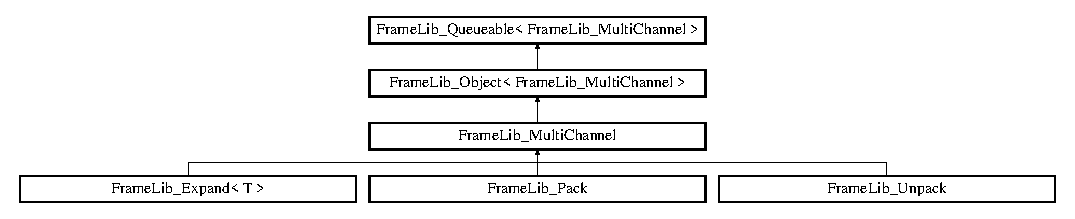
\includegraphics[height=2.715152cm]{class_frame_lib___multi_channel}
\end{center}
\end{figure}
\subsection*{Classes}
\begin{DoxyCompactItemize}
\item 
struct \hyperlink{struct_frame_lib___multi_channel_1_1_connection_info}{Connection\+Info}
\end{DoxyCompactItemize}
\subsection*{Public Member Functions}
\begin{DoxyCompactItemize}
\item 
\hyperlink{class_frame_lib___multi_channel_a77a5841c9d5efaae5bba85e23279a0de}{Frame\+Lib\+\_\+\+Multi\+Channel} (\hyperlink{_frame_lib___types_8h_a842c5e2e69277690b064bf363c017980}{Object\+Type} type, \hyperlink{class_frame_lib___context}{Frame\+Lib\+\_\+\+Context} context, unsigned long n\+Ins, unsigned long n\+Outs)
\item 
\hyperlink{class_frame_lib___multi_channel_aae7ab1c8e9db0c7bc6e26671e1ac4ab4}{Frame\+Lib\+\_\+\+Multi\+Channel} (\hyperlink{_frame_lib___types_8h_a842c5e2e69277690b064bf363c017980}{Object\+Type} type, \hyperlink{class_frame_lib___context}{Frame\+Lib\+\_\+\+Context} context)
\item 
virtual \hyperlink{class_frame_lib___multi_channel_ab6c1272cacfc7bf3cad1e2430d4c7020}{$\sim$\+Frame\+Lib\+\_\+\+Multi\+Channel} ()
\item 
virtual void \hyperlink{class_frame_lib___multi_channel_a2bbd1050ff53556bf671282312857301}{set\+Fixed\+Input} (unsigned long idx, double $\ast$input, unsigned long size)
\item 
virtual void \hyperlink{class_frame_lib___multi_channel_a8ad8f1c0138f32ef0bfb7e4673b34d30}{block\+Update} (double $\ast$$\ast$ins, double $\ast$$\ast$outs, unsigned long \hyperlink{_frame_lib___memory_8cpp_a8ef7d53a4cac28bf580a61f265fcaaa6}{block\+Size})
\item 
virtual void \hyperlink{class_frame_lib___multi_channel_af27f3dca507c48459452be825b4c0c72}{reset} (double sampling\+Rate, unsigned long max\+Block\+Size)
\item 
virtual void \hyperlink{class_frame_lib___multi_channel_ad8b21345a7b864a48060d2475af2fe1e}{delete\+Connection} (unsigned long in\+Idx)
\item 
virtual void \hyperlink{class_frame_lib___multi_channel_ab610f5adf0eb5b287a4a81806ce9b528}{add\+Connection} (\hyperlink{class_frame_lib___multi_channel}{Frame\+Lib\+\_\+\+Multi\+Channel} $\ast$object, unsigned long out\+Idx, unsigned long in\+Idx)
\item 
virtual void \hyperlink{class_frame_lib___multi_channel_aa7dfda2331a430b0db3f43d3bde293aa}{clear\+Connections} ()
\item 
virtual bool \hyperlink{class_frame_lib___multi_channel_a25159857f4088cf179c1d7c3d62cac76}{is\+Connected} (unsigned long in\+Idx)
\end{DoxyCompactItemize}
\subsection*{Static Public Member Functions}
\begin{DoxyCompactItemize}
\item 
static bool \hyperlink{class_frame_lib___multi_channel_a2995ef0ba184b2d8a1c44b74f5f39876}{handles\+Audio} ()
\end{DoxyCompactItemize}
\subsection*{Protected Member Functions}
\begin{DoxyCompactItemize}
\item 
void \hyperlink{class_frame_lib___multi_channel_aa602f450561447330df32fe73167244b}{set\+IO} (unsigned long n\+Ins, unsigned long n\+Outs, unsigned long n\+Audio\+Chans=0)
\item 
unsigned long \hyperlink{class_frame_lib___multi_channel_a8ba357b72ac5103d936e7416384294e0}{get\+Input\+Num\+Chans} (unsigned long in\+Idx)
\item 
\hyperlink{struct_frame_lib___multi_channel_1_1_connection_info}{Connection\+Info} \hyperlink{class_frame_lib___multi_channel_a484bbcd67d139f4166c1b731e63d3b92}{get\+Input\+Chan} (unsigned long in\+Idx, unsigned long chan)
\end{DoxyCompactItemize}
\subsection*{Protected Attributes}
\begin{DoxyCompactItemize}
\item 
std\+::vector$<$ Multi\+Channel\+Output $>$ \hyperlink{class_frame_lib___multi_channel_a2d993bc32c4625a1adbd84997c5d74f2}{m\+Outputs}
\end{DoxyCompactItemize}


\subsection{Constructor \& Destructor Documentation}
\mbox{\Hypertarget{class_frame_lib___multi_channel_a77a5841c9d5efaae5bba85e23279a0de}\label{class_frame_lib___multi_channel_a77a5841c9d5efaae5bba85e23279a0de}} 
\index{Frame\+Lib\+\_\+\+Multi\+Channel@{Frame\+Lib\+\_\+\+Multi\+Channel}!Frame\+Lib\+\_\+\+Multi\+Channel@{Frame\+Lib\+\_\+\+Multi\+Channel}}
\index{Frame\+Lib\+\_\+\+Multi\+Channel@{Frame\+Lib\+\_\+\+Multi\+Channel}!Frame\+Lib\+\_\+\+Multi\+Channel@{Frame\+Lib\+\_\+\+Multi\+Channel}}
\subsubsection{\texorpdfstring{Frame\+Lib\+\_\+\+Multi\+Channel()}{FrameLib\_MultiChannel()}\hspace{0.1cm}{\footnotesize\ttfamily [1/2]}}
{\footnotesize\ttfamily Frame\+Lib\+\_\+\+Multi\+Channel\+::\+Frame\+Lib\+\_\+\+Multi\+Channel (\begin{DoxyParamCaption}\item[{\hyperlink{_frame_lib___types_8h_a842c5e2e69277690b064bf363c017980}{Object\+Type}}]{type,  }\item[{\hyperlink{class_frame_lib___context}{Frame\+Lib\+\_\+\+Context}}]{context,  }\item[{unsigned long}]{n\+Ins,  }\item[{unsigned long}]{n\+Outs }\end{DoxyParamCaption})\hspace{0.3cm}{\ttfamily [inline]}}

\mbox{\Hypertarget{class_frame_lib___multi_channel_aae7ab1c8e9db0c7bc6e26671e1ac4ab4}\label{class_frame_lib___multi_channel_aae7ab1c8e9db0c7bc6e26671e1ac4ab4}} 
\index{Frame\+Lib\+\_\+\+Multi\+Channel@{Frame\+Lib\+\_\+\+Multi\+Channel}!Frame\+Lib\+\_\+\+Multi\+Channel@{Frame\+Lib\+\_\+\+Multi\+Channel}}
\index{Frame\+Lib\+\_\+\+Multi\+Channel@{Frame\+Lib\+\_\+\+Multi\+Channel}!Frame\+Lib\+\_\+\+Multi\+Channel@{Frame\+Lib\+\_\+\+Multi\+Channel}}
\subsubsection{\texorpdfstring{Frame\+Lib\+\_\+\+Multi\+Channel()}{FrameLib\_MultiChannel()}\hspace{0.1cm}{\footnotesize\ttfamily [2/2]}}
{\footnotesize\ttfamily Frame\+Lib\+\_\+\+Multi\+Channel\+::\+Frame\+Lib\+\_\+\+Multi\+Channel (\begin{DoxyParamCaption}\item[{\hyperlink{_frame_lib___types_8h_a842c5e2e69277690b064bf363c017980}{Object\+Type}}]{type,  }\item[{\hyperlink{class_frame_lib___context}{Frame\+Lib\+\_\+\+Context}}]{context }\end{DoxyParamCaption})\hspace{0.3cm}{\ttfamily [inline]}}

\mbox{\Hypertarget{class_frame_lib___multi_channel_ab6c1272cacfc7bf3cad1e2430d4c7020}\label{class_frame_lib___multi_channel_ab6c1272cacfc7bf3cad1e2430d4c7020}} 
\index{Frame\+Lib\+\_\+\+Multi\+Channel@{Frame\+Lib\+\_\+\+Multi\+Channel}!````~Frame\+Lib\+\_\+\+Multi\+Channel@{$\sim$\+Frame\+Lib\+\_\+\+Multi\+Channel}}
\index{````~Frame\+Lib\+\_\+\+Multi\+Channel@{$\sim$\+Frame\+Lib\+\_\+\+Multi\+Channel}!Frame\+Lib\+\_\+\+Multi\+Channel@{Frame\+Lib\+\_\+\+Multi\+Channel}}
\subsubsection{\texorpdfstring{$\sim$\+Frame\+Lib\+\_\+\+Multi\+Channel()}{~FrameLib\_MultiChannel()}}
{\footnotesize\ttfamily virtual Frame\+Lib\+\_\+\+Multi\+Channel\+::$\sim$\+Frame\+Lib\+\_\+\+Multi\+Channel (\begin{DoxyParamCaption}{ }\end{DoxyParamCaption})\hspace{0.3cm}{\ttfamily [inline]}, {\ttfamily [virtual]}}



\subsection{Member Function Documentation}
\mbox{\Hypertarget{class_frame_lib___multi_channel_ab610f5adf0eb5b287a4a81806ce9b528}\label{class_frame_lib___multi_channel_ab610f5adf0eb5b287a4a81806ce9b528}} 
\index{Frame\+Lib\+\_\+\+Multi\+Channel@{Frame\+Lib\+\_\+\+Multi\+Channel}!add\+Connection@{add\+Connection}}
\index{add\+Connection@{add\+Connection}!Frame\+Lib\+\_\+\+Multi\+Channel@{Frame\+Lib\+\_\+\+Multi\+Channel}}
\subsubsection{\texorpdfstring{add\+Connection()}{addConnection()}}
{\footnotesize\ttfamily void Frame\+Lib\+\_\+\+Multi\+Channel\+::add\+Connection (\begin{DoxyParamCaption}\item[{\hyperlink{class_frame_lib___multi_channel}{Frame\+Lib\+\_\+\+Multi\+Channel} $\ast$}]{object,  }\item[{unsigned long}]{out\+Idx,  }\item[{unsigned long}]{in\+Idx }\end{DoxyParamCaption})\hspace{0.3cm}{\ttfamily [virtual]}}



Implements \hyperlink{class_frame_lib___object_ab276c500466359bb43494ff2b7c94cc6}{Frame\+Lib\+\_\+\+Object$<$ Frame\+Lib\+\_\+\+Multi\+Channel $>$}.

\mbox{\Hypertarget{class_frame_lib___multi_channel_a8ad8f1c0138f32ef0bfb7e4673b34d30}\label{class_frame_lib___multi_channel_a8ad8f1c0138f32ef0bfb7e4673b34d30}} 
\index{Frame\+Lib\+\_\+\+Multi\+Channel@{Frame\+Lib\+\_\+\+Multi\+Channel}!block\+Update@{block\+Update}}
\index{block\+Update@{block\+Update}!Frame\+Lib\+\_\+\+Multi\+Channel@{Frame\+Lib\+\_\+\+Multi\+Channel}}
\subsubsection{\texorpdfstring{block\+Update()}{blockUpdate()}}
{\footnotesize\ttfamily virtual void Frame\+Lib\+\_\+\+Multi\+Channel\+::block\+Update (\begin{DoxyParamCaption}\item[{double $\ast$$\ast$}]{ins,  }\item[{double $\ast$$\ast$}]{outs,  }\item[{unsigned long}]{block\+Size }\end{DoxyParamCaption})\hspace{0.3cm}{\ttfamily [inline]}, {\ttfamily [virtual]}}



Implements \hyperlink{class_frame_lib___object_a6efd81ab386e62400960471fa3cc94e7}{Frame\+Lib\+\_\+\+Object$<$ Frame\+Lib\+\_\+\+Multi\+Channel $>$}.



Reimplemented in \hyperlink{class_frame_lib___expand_ae712d631cb99284e91c3f318534b3c03}{Frame\+Lib\+\_\+\+Expand$<$ T $>$}.

\mbox{\Hypertarget{class_frame_lib___multi_channel_aa7dfda2331a430b0db3f43d3bde293aa}\label{class_frame_lib___multi_channel_aa7dfda2331a430b0db3f43d3bde293aa}} 
\index{Frame\+Lib\+\_\+\+Multi\+Channel@{Frame\+Lib\+\_\+\+Multi\+Channel}!clear\+Connections@{clear\+Connections}}
\index{clear\+Connections@{clear\+Connections}!Frame\+Lib\+\_\+\+Multi\+Channel@{Frame\+Lib\+\_\+\+Multi\+Channel}}
\subsubsection{\texorpdfstring{clear\+Connections()}{clearConnections()}}
{\footnotesize\ttfamily void Frame\+Lib\+\_\+\+Multi\+Channel\+::clear\+Connections (\begin{DoxyParamCaption}{ }\end{DoxyParamCaption})\hspace{0.3cm}{\ttfamily [virtual]}}



Implements \hyperlink{class_frame_lib___object_a5b219c0cb96a7b6b1f0c471f665337ec}{Frame\+Lib\+\_\+\+Object$<$ Frame\+Lib\+\_\+\+Multi\+Channel $>$}.

\mbox{\Hypertarget{class_frame_lib___multi_channel_ad8b21345a7b864a48060d2475af2fe1e}\label{class_frame_lib___multi_channel_ad8b21345a7b864a48060d2475af2fe1e}} 
\index{Frame\+Lib\+\_\+\+Multi\+Channel@{Frame\+Lib\+\_\+\+Multi\+Channel}!delete\+Connection@{delete\+Connection}}
\index{delete\+Connection@{delete\+Connection}!Frame\+Lib\+\_\+\+Multi\+Channel@{Frame\+Lib\+\_\+\+Multi\+Channel}}
\subsubsection{\texorpdfstring{delete\+Connection()}{deleteConnection()}}
{\footnotesize\ttfamily void Frame\+Lib\+\_\+\+Multi\+Channel\+::delete\+Connection (\begin{DoxyParamCaption}\item[{unsigned long}]{in\+Idx }\end{DoxyParamCaption})\hspace{0.3cm}{\ttfamily [virtual]}}



Implements \hyperlink{class_frame_lib___object_a4ed6892941c7b68c885b38c202f336b3}{Frame\+Lib\+\_\+\+Object$<$ Frame\+Lib\+\_\+\+Multi\+Channel $>$}.

\mbox{\Hypertarget{class_frame_lib___multi_channel_a484bbcd67d139f4166c1b731e63d3b92}\label{class_frame_lib___multi_channel_a484bbcd67d139f4166c1b731e63d3b92}} 
\index{Frame\+Lib\+\_\+\+Multi\+Channel@{Frame\+Lib\+\_\+\+Multi\+Channel}!get\+Input\+Chan@{get\+Input\+Chan}}
\index{get\+Input\+Chan@{get\+Input\+Chan}!Frame\+Lib\+\_\+\+Multi\+Channel@{Frame\+Lib\+\_\+\+Multi\+Channel}}
\subsubsection{\texorpdfstring{get\+Input\+Chan()}{getInputChan()}}
{\footnotesize\ttfamily \hyperlink{struct_frame_lib___multi_channel_1_1_connection_info}{Connection\+Info} Frame\+Lib\+\_\+\+Multi\+Channel\+::get\+Input\+Chan (\begin{DoxyParamCaption}\item[{unsigned long}]{in\+Idx,  }\item[{unsigned long}]{chan }\end{DoxyParamCaption})\hspace{0.3cm}{\ttfamily [inline]}, {\ttfamily [protected]}}

\mbox{\Hypertarget{class_frame_lib___multi_channel_a8ba357b72ac5103d936e7416384294e0}\label{class_frame_lib___multi_channel_a8ba357b72ac5103d936e7416384294e0}} 
\index{Frame\+Lib\+\_\+\+Multi\+Channel@{Frame\+Lib\+\_\+\+Multi\+Channel}!get\+Input\+Num\+Chans@{get\+Input\+Num\+Chans}}
\index{get\+Input\+Num\+Chans@{get\+Input\+Num\+Chans}!Frame\+Lib\+\_\+\+Multi\+Channel@{Frame\+Lib\+\_\+\+Multi\+Channel}}
\subsubsection{\texorpdfstring{get\+Input\+Num\+Chans()}{getInputNumChans()}}
{\footnotesize\ttfamily unsigned long Frame\+Lib\+\_\+\+Multi\+Channel\+::get\+Input\+Num\+Chans (\begin{DoxyParamCaption}\item[{unsigned long}]{in\+Idx }\end{DoxyParamCaption})\hspace{0.3cm}{\ttfamily [protected]}}

\mbox{\Hypertarget{class_frame_lib___multi_channel_a2995ef0ba184b2d8a1c44b74f5f39876}\label{class_frame_lib___multi_channel_a2995ef0ba184b2d8a1c44b74f5f39876}} 
\index{Frame\+Lib\+\_\+\+Multi\+Channel@{Frame\+Lib\+\_\+\+Multi\+Channel}!handles\+Audio@{handles\+Audio}}
\index{handles\+Audio@{handles\+Audio}!Frame\+Lib\+\_\+\+Multi\+Channel@{Frame\+Lib\+\_\+\+Multi\+Channel}}
\subsubsection{\texorpdfstring{handles\+Audio()}{handlesAudio()}}
{\footnotesize\ttfamily static bool Frame\+Lib\+\_\+\+Multi\+Channel\+::handles\+Audio (\begin{DoxyParamCaption}{ }\end{DoxyParamCaption})\hspace{0.3cm}{\ttfamily [inline]}, {\ttfamily [static]}}

\mbox{\Hypertarget{class_frame_lib___multi_channel_a25159857f4088cf179c1d7c3d62cac76}\label{class_frame_lib___multi_channel_a25159857f4088cf179c1d7c3d62cac76}} 
\index{Frame\+Lib\+\_\+\+Multi\+Channel@{Frame\+Lib\+\_\+\+Multi\+Channel}!is\+Connected@{is\+Connected}}
\index{is\+Connected@{is\+Connected}!Frame\+Lib\+\_\+\+Multi\+Channel@{Frame\+Lib\+\_\+\+Multi\+Channel}}
\subsubsection{\texorpdfstring{is\+Connected()}{isConnected()}}
{\footnotesize\ttfamily bool Frame\+Lib\+\_\+\+Multi\+Channel\+::is\+Connected (\begin{DoxyParamCaption}\item[{unsigned long}]{in\+Idx }\end{DoxyParamCaption})\hspace{0.3cm}{\ttfamily [virtual]}}



Implements \hyperlink{class_frame_lib___object_a773123ebc7b3571e607cb1a6c4296d20}{Frame\+Lib\+\_\+\+Object$<$ Frame\+Lib\+\_\+\+Multi\+Channel $>$}.

\mbox{\Hypertarget{class_frame_lib___multi_channel_af27f3dca507c48459452be825b4c0c72}\label{class_frame_lib___multi_channel_af27f3dca507c48459452be825b4c0c72}} 
\index{Frame\+Lib\+\_\+\+Multi\+Channel@{Frame\+Lib\+\_\+\+Multi\+Channel}!reset@{reset}}
\index{reset@{reset}!Frame\+Lib\+\_\+\+Multi\+Channel@{Frame\+Lib\+\_\+\+Multi\+Channel}}
\subsubsection{\texorpdfstring{reset()}{reset()}}
{\footnotesize\ttfamily virtual void Frame\+Lib\+\_\+\+Multi\+Channel\+::reset (\begin{DoxyParamCaption}\item[{double}]{sampling\+Rate,  }\item[{unsigned long}]{max\+Block\+Size }\end{DoxyParamCaption})\hspace{0.3cm}{\ttfamily [inline]}, {\ttfamily [virtual]}}



Implements \hyperlink{class_frame_lib___object_aeb02311ab422dd569aeb982e31a66893}{Frame\+Lib\+\_\+\+Object$<$ Frame\+Lib\+\_\+\+Multi\+Channel $>$}.



Reimplemented in \hyperlink{class_frame_lib___expand_a579f16ec32e05ff84ee766038012fc3f}{Frame\+Lib\+\_\+\+Expand$<$ T $>$}.

\mbox{\Hypertarget{class_frame_lib___multi_channel_a2bbd1050ff53556bf671282312857301}\label{class_frame_lib___multi_channel_a2bbd1050ff53556bf671282312857301}} 
\index{Frame\+Lib\+\_\+\+Multi\+Channel@{Frame\+Lib\+\_\+\+Multi\+Channel}!set\+Fixed\+Input@{set\+Fixed\+Input}}
\index{set\+Fixed\+Input@{set\+Fixed\+Input}!Frame\+Lib\+\_\+\+Multi\+Channel@{Frame\+Lib\+\_\+\+Multi\+Channel}}
\subsubsection{\texorpdfstring{set\+Fixed\+Input()}{setFixedInput()}}
{\footnotesize\ttfamily virtual void Frame\+Lib\+\_\+\+Multi\+Channel\+::set\+Fixed\+Input (\begin{DoxyParamCaption}\item[{unsigned long}]{idx,  }\item[{double $\ast$}]{input,  }\item[{unsigned long}]{size }\end{DoxyParamCaption})\hspace{0.3cm}{\ttfamily [inline]}, {\ttfamily [virtual]}}



Implements \hyperlink{class_frame_lib___object_a0d3bed42a21ebf248366f4457722beff}{Frame\+Lib\+\_\+\+Object$<$ Frame\+Lib\+\_\+\+Multi\+Channel $>$}.



Reimplemented in \hyperlink{class_frame_lib___expand_a73f7bf4264d45f56f249d6303b3e4c35}{Frame\+Lib\+\_\+\+Expand$<$ T $>$}.

\mbox{\Hypertarget{class_frame_lib___multi_channel_aa602f450561447330df32fe73167244b}\label{class_frame_lib___multi_channel_aa602f450561447330df32fe73167244b}} 
\index{Frame\+Lib\+\_\+\+Multi\+Channel@{Frame\+Lib\+\_\+\+Multi\+Channel}!set\+IO@{set\+IO}}
\index{set\+IO@{set\+IO}!Frame\+Lib\+\_\+\+Multi\+Channel@{Frame\+Lib\+\_\+\+Multi\+Channel}}
\subsubsection{\texorpdfstring{set\+I\+O()}{setIO()}}
{\footnotesize\ttfamily void Frame\+Lib\+\_\+\+Multi\+Channel\+::set\+IO (\begin{DoxyParamCaption}\item[{unsigned long}]{n\+Ins,  }\item[{unsigned long}]{n\+Outs,  }\item[{unsigned long}]{n\+Audio\+Chans = {\ttfamily 0} }\end{DoxyParamCaption})\hspace{0.3cm}{\ttfamily [inline]}, {\ttfamily [protected]}}



\subsection{Member Data Documentation}
\mbox{\Hypertarget{class_frame_lib___multi_channel_a2d993bc32c4625a1adbd84997c5d74f2}\label{class_frame_lib___multi_channel_a2d993bc32c4625a1adbd84997c5d74f2}} 
\index{Frame\+Lib\+\_\+\+Multi\+Channel@{Frame\+Lib\+\_\+\+Multi\+Channel}!m\+Outputs@{m\+Outputs}}
\index{m\+Outputs@{m\+Outputs}!Frame\+Lib\+\_\+\+Multi\+Channel@{Frame\+Lib\+\_\+\+Multi\+Channel}}
\subsubsection{\texorpdfstring{m\+Outputs}{mOutputs}}
{\footnotesize\ttfamily std\+::vector$<$Multi\+Channel\+Output$>$ Frame\+Lib\+\_\+\+Multi\+Channel\+::m\+Outputs\hspace{0.3cm}{\ttfamily [protected]}}



The documentation for this class was generated from the following files\+:\begin{DoxyCompactItemize}
\item 
Frame\+Lib\+\_\+\+Framework/\hyperlink{_frame_lib___multichannel_8h}{Frame\+Lib\+\_\+\+Multichannel.\+h}\item 
Frame\+Lib\+\_\+\+Framework/\hyperlink{_frame_lib___multichannel_8cpp}{Frame\+Lib\+\_\+\+Multichannel.\+cpp}\end{DoxyCompactItemize}

\hypertarget{class_frame_lib___object}{}\section{Frame\+Lib\+\_\+\+Object$<$ T $>$ Class Template Reference}
\label{class_frame_lib___object}\index{Frame\+Lib\+\_\+\+Object$<$ T $>$@{Frame\+Lib\+\_\+\+Object$<$ T $>$}}


an abstract template class providing an interface for Frame\+Lib objects and implementing connectivity  




{\ttfamily \#include $<$Frame\+Lib\+\_\+\+Object.\+h$>$}

Inheritance diagram for Frame\+Lib\+\_\+\+Object$<$ T $>$\+:\begin{figure}[H]
\begin{center}
\leavevmode
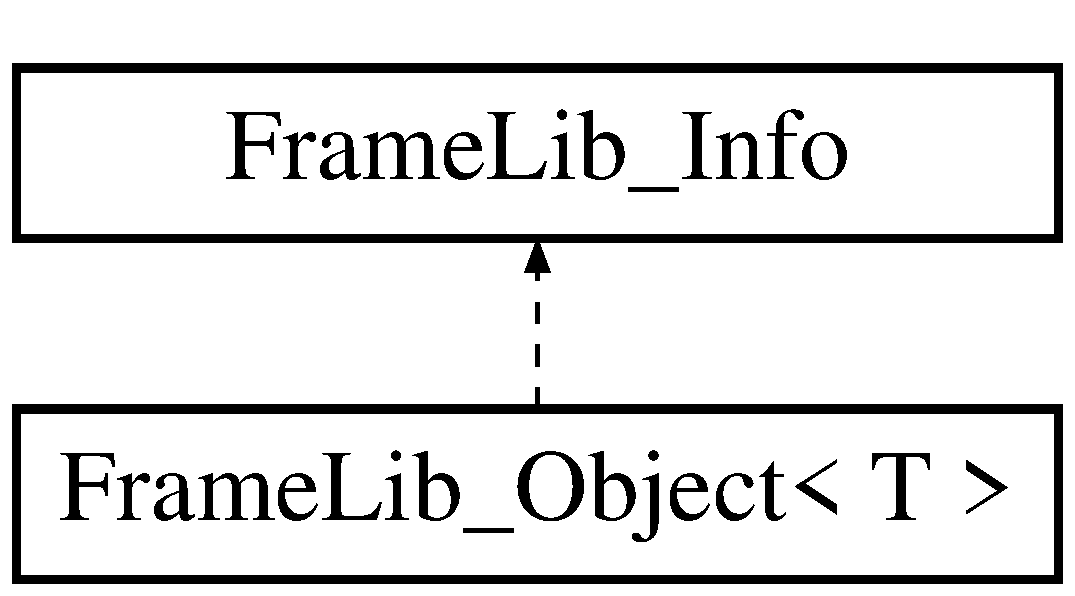
\includegraphics[height=2.000000cm]{class_frame_lib___object}
\end{center}
\end{figure}
\subsection*{Classes}
\begin{DoxyCompactItemize}
\item 
class \hyperlink{struct_frame_lib___object_1_1_connection}{Connection}
\begin{DoxyCompactList}\small\item\em holds the connected object and IO indices for a connection to an object \end{DoxyCompactList}\end{DoxyCompactItemize}
\subsection*{Public Types}
\begin{DoxyCompactItemize}
\item 
using \hyperlink{class_frame_lib___object_a3e6fce9a979bf08406e40e51583cb4ea}{Queue} = typename \hyperlink{class_frame_lib___queueable}{Frame\+Lib\+\_\+\+Queueable}$<$ T $>$\+::\hyperlink{class_frame_lib___object_a3e6fce9a979bf08406e40e51583cb4ea}{Queue}
\end{DoxyCompactItemize}
\subsection*{Public Member Functions}
\begin{DoxyCompactItemize}
\item 
\hyperlink{class_frame_lib___object_ae377e7fd8ca51210af511a9fdc2544e7}{Frame\+Lib\+\_\+\+Object} (\hyperlink{_frame_lib___types_8h_a842c5e2e69277690b064bf363c017980}{Object\+Type} type, \hyperlink{class_frame_lib___context}{Frame\+Lib\+\_\+\+Context} context, \hyperlink{struct_frame_lib___proxy}{Frame\+Lib\+\_\+\+Proxy} $\ast$proxy)
\item 
virtual \hyperlink{class_frame_lib___object_ab88bcc3fe9e1c9da41a4afebb3d05005}{$\sim$\+Frame\+Lib\+\_\+\+Object} ()
\item 
\hyperlink{_frame_lib___types_8h_a842c5e2e69277690b064bf363c017980}{Object\+Type} \hyperlink{class_frame_lib___object_a8d96d1f55054e583a99891ad65f84a3a}{get\+Type} () const
\item 
\hyperlink{class_frame_lib___context}{Frame\+Lib\+\_\+\+Context} \hyperlink{class_frame_lib___object_a8f636902888847c78cf16d74717bd861}{get\+Context} () const
\item 
\hyperlink{struct_frame_lib___proxy}{Frame\+Lib\+\_\+\+Proxy} $\ast$ \hyperlink{class_frame_lib___object_a9aa8f7f487999748f04c39ea2692a8ed}{get\+Proxy} () const
\item 
unsigned long \hyperlink{class_frame_lib___object_a310416236585b52c2de1c47a9aa64b02}{get\+Num\+Ins} () const
\item 
unsigned long \hyperlink{class_frame_lib___object_a255f6ae814dbb946d445ef244dd39975}{get\+Num\+Outs} () const
\item 
unsigned long \hyperlink{class_frame_lib___object_ad29b6281916a933c5baa43cbb7d11efd}{get\+Num\+Audio\+Ins} () const
\item 
unsigned long \hyperlink{class_frame_lib___object_a430c0531a4c38ad49a556af1cca0af88}{get\+Num\+Audio\+Outs} () const
\item 
unsigned long \hyperlink{class_frame_lib___object_a59e6e7dba2d18444be6d5fbee15c73f2}{get\+Num\+Audio\+Chans} () const
\item 
virtual void \hyperlink{class_frame_lib___object_a0d3bed42a21ebf248366f4457722beff}{set\+Fixed\+Input} (unsigned long idx, double $\ast$input, unsigned long size)=0
\item 
virtual const double $\ast$ \hyperlink{class_frame_lib___object_ab34877668c8b6a2ca5efa6bc10368820}{get\+Fixed\+Input} (unsigned long idx, unsigned long $\ast$size)=0
\item 
virtual void \hyperlink{class_frame_lib___object_abd8e6ba645082041000b7a0b67c9b011}{block\+Update} (const double $\ast$const $\ast$ins, double $\ast$$\ast$outs, unsigned long \hyperlink{_frame_lib___memory_8cpp_a8ef7d53a4cac28bf580a61f265fcaaa6}{block\+Size})=0
\item 
virtual void \hyperlink{class_frame_lib___object_aeb02311ab422dd569aeb982e31a66893}{reset} (double sampling\+Rate, unsigned long max\+Block\+Size)=0
\item 
virtual std\+::string \hyperlink{class_frame_lib___object_a10d673de9a3c59ace6a22ba1cff313c8}{object\+Info} (bool verbose=false)
\item 
virtual std\+::string \hyperlink{class_frame_lib___object_a49abea5f18125c425b1eae8710735891}{input\+Info} (unsigned long idx, bool verbose=false)
\item 
virtual std\+::string \hyperlink{class_frame_lib___object_a6e6d79e8d620eedbaa50abf324cdedf5}{output\+Info} (unsigned long idx, bool verbose=false)
\item 
virtual std\+::string \hyperlink{class_frame_lib___object_af618fcdec82b457911147c7c293bedd7}{audio\+Info} (unsigned long idx, bool verbose=false)
\item 
virtual \hyperlink{_frame_lib___types_8h_ad495a9f61af7fff07d7e97979d1ab854}{Frame\+Type} \hyperlink{class_frame_lib___object_ab1ab1ae8180bb8b7e881aac6a4e1066c}{input\+Type} (unsigned long idx) const =0
\item 
virtual \hyperlink{_frame_lib___types_8h_ad495a9f61af7fff07d7e97979d1ab854}{Frame\+Type} \hyperlink{class_frame_lib___object_a03eb408844f15d8f73cee67f43149b9d}{output\+Type} (unsigned long idx) const =0
\item 
virtual const \hyperlink{class_frame_lib___parameters}{Frame\+Lib\+\_\+\+Parameters} $\ast$ \hyperlink{class_frame_lib___object_ac90a6770aeef26ee1601889dc16dba56}{get\+Parameters} () const
\item 
\hyperlink{_frame_lib___types_8h_a2a427ca8c6f961bac8e41f6edecf0722}{Connection\+Result} \hyperlink{class_frame_lib___object_a53722775485e80ba9590750ad68e437b}{add\+Connection} (\hyperlink{struct_frame_lib___object_1_1_connection}{Connection} connection, unsigned long in\+Idx)
\item 
void \hyperlink{class_frame_lib___object_aa7dbc1735ebd68008abd939d50edce49}{delete\+Connection} (unsigned long in\+Idx)
\item 
\hyperlink{_frame_lib___types_8h_a2a427ca8c6f961bac8e41f6edecf0722}{Connection\+Result} \hyperlink{class_frame_lib___object_aaa1ec62334620a049632f72ad2c22538}{add\+Ordering\+Connection} (\hyperlink{struct_frame_lib___object_1_1_connection}{Connection} connection)
\item 
void \hyperlink{class_frame_lib___object_ab2951a9798e792517aac61ba27553159}{delete\+Ordering\+Connection} (\hyperlink{struct_frame_lib___object_1_1_connection}{Connection} connection)
\item 
void \hyperlink{class_frame_lib___object_abd548d2e3899a1a8738a71b3824ac039}{clear\+Ordering\+Connections} ()
\item 
void \hyperlink{class_frame_lib___object_a4fa6add369fd21ddc5250efd740d0285}{clear\+Connections} ()
\item 
\hyperlink{_frame_lib___types_8h_a2a427ca8c6f961bac8e41f6edecf0722}{Connection\+Result} \hyperlink{class_frame_lib___object_a7a1b43b3eda170fbf298b2dfe94f9aa3}{set\+Input\+Alias} (\hyperlink{struct_frame_lib___object_1_1_connection}{Connection} alias, unsigned long in\+Idx)
\item 
\hyperlink{_frame_lib___types_8h_a2a427ca8c6f961bac8e41f6edecf0722}{Connection\+Result} \hyperlink{class_frame_lib___object_a8455782f3ba8037eb07b0d08ca6c59c2}{set\+Ordering\+Alias} (T $\ast$alias)
\item 
\hyperlink{_frame_lib___types_8h_a2a427ca8c6f961bac8e41f6edecf0722}{Connection\+Result} \hyperlink{class_frame_lib___object_a689936615ffd3902f29eec957703f83c}{set\+Output\+Alias} (\hyperlink{struct_frame_lib___object_1_1_connection}{Connection} alias, unsigned long out\+Idx)
\item 
bool \hyperlink{class_frame_lib___object_a2b4ed60a6032ff9fab191fcb492ef404}{is\+Connected} (unsigned long in\+Idx) const
\item 
\hyperlink{struct_frame_lib___object_1_1_connection}{Connection} \hyperlink{class_frame_lib___object_a87d56a68ea04f515206adb616b233048}{get\+Connection} (unsigned long in\+Idx) const
\item 
bool \hyperlink{class_frame_lib___object_a0f0baead3c4ca259a6b4e7a417f45735}{supports\+Ordering\+Connections} () const
\item 
unsigned long \hyperlink{class_frame_lib___object_ace330616fd3334122babc5901b758d28}{get\+Num\+Ordering\+Connections} () const
\item 
\hyperlink{struct_frame_lib___object_1_1_connection}{Connection} \hyperlink{class_frame_lib___object_ad67d23eb04120b30c16b0a213b3d3303}{get\+Ordering\+Connection} (unsigned long idx) const
\item 
virtual void \hyperlink{class_frame_lib___object_afa5bb93302a641c23b5eac7ab0dfe516}{auto\+Ordering\+Connections} ()=0
\item 
virtual void \hyperlink{class_frame_lib___object_aac43ebfacb59081f7f60957380df7481}{clear\+Auto\+Ordering\+Connections} ()=0
\item 
void \hyperlink{class_frame_lib___object_add88ac11ac70eb93b2d05eebf2ab9b82}{call\+Connection\+Update} ()
\item 
{\footnotesize template$<$class U $>$ }\\void \hyperlink{class_frame_lib___object_a9b2213d1010d13c7c79de5d5f053ea1b}{add\+Output\+Dependencies} (std\+::vector$<$ U $\ast$$>$ \&dependencies)
\item 
{\footnotesize template$<$class U $>$ }\\void \hyperlink{class_frame_lib___object_a8da8cac4a5c6f6fcdbfe50e1abd186b0}{add\+Output\+Dependencies} (std\+::vector$<$ U $\ast$$>$ \&dependencies, unsigned long out\+Idx)
\end{DoxyCompactItemize}
\subsection*{Static Public Member Functions}
\begin{DoxyCompactItemize}
\item 
static bool \hyperlink{class_frame_lib___object_a3d8517596d7598585c08af375dae79b9}{handles\+Audio} ()
\end{DoxyCompactItemize}
\subsection*{Protected Member Functions}
\begin{DoxyCompactItemize}
\item 
\hyperlink{struct_frame_lib___object_1_1_connection}{Connection} \hyperlink{class_frame_lib___object_acd33f63f6755575ad4eebabe6b7e2aaa}{get\+Connection\+Internal} (unsigned long in\+Idx) const
\item 
\hyperlink{struct_frame_lib___object_1_1_connection}{Connection} \hyperlink{class_frame_lib___object_ac6075f11200b91f9a133344190a64dc4}{get\+Ordering\+Connection\+Internal} (unsigned long idx) const
\item 
void \hyperlink{class_frame_lib___object_ac59c8a2828c43887ee4093fb1cbe3f9a}{add\+Output\+Dependencies} (\hyperlink{class_frame_lib___object_a3e6fce9a979bf08406e40e51583cb4ea}{Queue} $\ast$queue)
\item 
void \hyperlink{class_frame_lib___object_aaf9637ffd5654f73014c2750cfa54bae}{add\+Output\+Dependencies} (\hyperlink{class_frame_lib___object_a3e6fce9a979bf08406e40e51583cb4ea}{Queue} $\ast$queue, unsigned long out\+Idx)
\item 
void \hyperlink{class_frame_lib___object_a5c34227ace795af7da847fff3f2b300d}{set\+IO} (unsigned long n\+Ins, unsigned long n\+Outs, unsigned long n\+Audio\+Chans=0)
\item 
void \hyperlink{class_frame_lib___object_a60dba6cd7148c3223adb4197d6712839}{enable\+Ordering\+Connections} ()
\item 
{\footnotesize template$<$class U $>$ }\\U $\ast$ \hyperlink{class_frame_lib___object_a32ba9cf8b728317fc92c10310ab83e67}{alloc} (unsigned long N)
\item 
{\footnotesize template$<$class U $>$ }\\void \hyperlink{class_frame_lib___object_ab42be79621db7363ca4a34f63704d04f}{dealloc} (U $\ast$\&ptr)
\item 
void \hyperlink{class_frame_lib___object_a33b99de2c7a35227bc8a40d4c3b2ee76}{clear\+Allocator} ()
\item 
\hyperlink{class_frame_lib___local_allocator_1_1_storage}{Frame\+Lib\+\_\+\+Local\+Allocator\+::\+Storage} $\ast$ \hyperlink{class_frame_lib___object_a316d15b17757ddfef4341d0f8afe443e}{register\+Storage} (const char $\ast$name)
\item 
void \hyperlink{class_frame_lib___object_a4c131dff9d634f17696fb3ae6be06e9b}{release\+Storage} (\hyperlink{class_frame_lib___local_allocator_1_1_storage}{Frame\+Lib\+\_\+\+Local\+Allocator\+::\+Storage} $\ast$\&storage)
\item 
const double $\ast$ \hyperlink{class_frame_lib___object_a604899fbd09fd9b37502ecb07a831b30}{get\+Empty\+Fixed\+Input} (unsigned long idx, unsigned long $\ast$size)
\end{DoxyCompactItemize}
\subsection*{Static Protected Member Functions}
\begin{DoxyCompactItemize}
\item 
static const char $\ast$ \hyperlink{class_frame_lib___object_a2cb965a15f4634a5fdddc2b009005211}{format\+Info} (const char $\ast$verbose\+Str, const char $\ast$brief\+Str, bool verbose)
\item 
static std\+::string \hyperlink{class_frame_lib___object_ab11cf702a6158f0cd9952ceaaf6c4952}{format\+Info} (const char $\ast$str, unsigned long idx)
\item 
static std\+::string \hyperlink{class_frame_lib___object_aa30676408b8f8161894eb0e533a8522b}{format\+Info} (const char $\ast$verbose\+Str, const char $\ast$brief\+Str, unsigned long idx, bool verbose)
\item 
static std\+::string \hyperlink{class_frame_lib___object_a784bf34c1ef238872b64b9668e23de28}{format\+Info} (const char $\ast$str, const char $\ast$replace\+Str)
\item 
static std\+::string \hyperlink{class_frame_lib___object_a7babe2dd654fbd0c8c05eb7f7ea31550}{format\+Info} (const char $\ast$verbose\+Str, const char $\ast$brief\+Str, const char $\ast$replace\+Str, bool verbose)
\item 
static std\+::string \hyperlink{class_frame_lib___object_a7c57bdfc3fa9a9bb34b607ffa240d47e}{parameter\+Input\+Info} (bool verbose)
\item 
static std\+::string \hyperlink{class_frame_lib___object_a26307f11e68962614da4178115e665b7}{numbered\+String} (const char $\ast$str, unsigned long idx)
\item 
{\footnotesize template$<$class U $>$ }\\static bool \hyperlink{class_frame_lib___object_aa06caf2148631c1a6c3204ac6d8b2bc7}{add\+Unique\+Item} (std\+::vector$<$ U $>$ \&list, U item)
\item 
{\footnotesize template$<$class U $>$ }\\static bool \hyperlink{class_frame_lib___object_aa3bdc91a5f12b72e57fbb010e1827f57}{delete\+Unique\+Item} (std\+::vector$<$ U $>$ \&list, U item)
\end{DoxyCompactItemize}


\subsection{Detailed Description}
\subsubsection*{template$<$class T$>$\newline
class Frame\+Lib\+\_\+\+Object$<$ T $>$}

an abstract template class providing an interface for Frame\+Lib objects and implementing connectivity 

\begin{DoxySeeAlso}{See also}
\hyperlink{class_frame_lib___block}{Frame\+Lib\+\_\+\+Block}, \hyperlink{class_frame_lib___d_s_p}{Frame\+Lib\+\_\+\+D\+SP} \hyperlink{class_frame_lib___multistream}{Frame\+Lib\+\_\+\+Multistream} 
\end{DoxySeeAlso}


\subsection{Member Typedef Documentation}
\mbox{\Hypertarget{class_frame_lib___object_a3e6fce9a979bf08406e40e51583cb4ea}\label{class_frame_lib___object_a3e6fce9a979bf08406e40e51583cb4ea}} 
\index{Frame\+Lib\+\_\+\+Object@{Frame\+Lib\+\_\+\+Object}!Queue@{Queue}}
\index{Queue@{Queue}!Frame\+Lib\+\_\+\+Object@{Frame\+Lib\+\_\+\+Object}}
\subsubsection{\texorpdfstring{Queue}{Queue}}
{\footnotesize\ttfamily template$<$class T$>$ \\
using \hyperlink{class_frame_lib___object}{Frame\+Lib\+\_\+\+Object}$<$ T $>$\+::\hyperlink{class_frame_lib___object_a3e6fce9a979bf08406e40e51583cb4ea}{Queue} =  typename \hyperlink{class_frame_lib___queueable}{Frame\+Lib\+\_\+\+Queueable}$<$T$>$\+::\hyperlink{class_frame_lib___object_a3e6fce9a979bf08406e40e51583cb4ea}{Queue}}



\subsection{Constructor \& Destructor Documentation}
\mbox{\Hypertarget{class_frame_lib___object_ae377e7fd8ca51210af511a9fdc2544e7}\label{class_frame_lib___object_ae377e7fd8ca51210af511a9fdc2544e7}} 
\index{Frame\+Lib\+\_\+\+Object@{Frame\+Lib\+\_\+\+Object}!Frame\+Lib\+\_\+\+Object@{Frame\+Lib\+\_\+\+Object}}
\index{Frame\+Lib\+\_\+\+Object@{Frame\+Lib\+\_\+\+Object}!Frame\+Lib\+\_\+\+Object@{Frame\+Lib\+\_\+\+Object}}
\subsubsection{\texorpdfstring{Frame\+Lib\+\_\+\+Object()}{FrameLib\_Object()}}
{\footnotesize\ttfamily template$<$class T$>$ \\
\hyperlink{class_frame_lib___object}{Frame\+Lib\+\_\+\+Object}$<$ T $>$\+::\hyperlink{class_frame_lib___object}{Frame\+Lib\+\_\+\+Object} (\begin{DoxyParamCaption}\item[{\hyperlink{_frame_lib___types_8h_a842c5e2e69277690b064bf363c017980}{Object\+Type}}]{type,  }\item[{\hyperlink{class_frame_lib___context}{Frame\+Lib\+\_\+\+Context}}]{context,  }\item[{\hyperlink{struct_frame_lib___proxy}{Frame\+Lib\+\_\+\+Proxy} $\ast$}]{proxy }\end{DoxyParamCaption})\hspace{0.3cm}{\ttfamily [inline]}}

\mbox{\Hypertarget{class_frame_lib___object_ab88bcc3fe9e1c9da41a4afebb3d05005}\label{class_frame_lib___object_ab88bcc3fe9e1c9da41a4afebb3d05005}} 
\index{Frame\+Lib\+\_\+\+Object@{Frame\+Lib\+\_\+\+Object}!````~Frame\+Lib\+\_\+\+Object@{$\sim$\+Frame\+Lib\+\_\+\+Object}}
\index{````~Frame\+Lib\+\_\+\+Object@{$\sim$\+Frame\+Lib\+\_\+\+Object}!Frame\+Lib\+\_\+\+Object@{Frame\+Lib\+\_\+\+Object}}
\subsubsection{\texorpdfstring{$\sim$\+Frame\+Lib\+\_\+\+Object()}{~FrameLib\_Object()}}
{\footnotesize\ttfamily template$<$class T$>$ \\
virtual \hyperlink{class_frame_lib___object}{Frame\+Lib\+\_\+\+Object}$<$ T $>$\+::$\sim$\hyperlink{class_frame_lib___object}{Frame\+Lib\+\_\+\+Object} (\begin{DoxyParamCaption}{ }\end{DoxyParamCaption})\hspace{0.3cm}{\ttfamily [inline]}, {\ttfamily [virtual]}}



\subsection{Member Function Documentation}
\mbox{\Hypertarget{class_frame_lib___object_a53722775485e80ba9590750ad68e437b}\label{class_frame_lib___object_a53722775485e80ba9590750ad68e437b}} 
\index{Frame\+Lib\+\_\+\+Object@{Frame\+Lib\+\_\+\+Object}!add\+Connection@{add\+Connection}}
\index{add\+Connection@{add\+Connection}!Frame\+Lib\+\_\+\+Object@{Frame\+Lib\+\_\+\+Object}}
\subsubsection{\texorpdfstring{add\+Connection()}{addConnection()}}
{\footnotesize\ttfamily template$<$class T$>$ \\
\hyperlink{_frame_lib___types_8h_a2a427ca8c6f961bac8e41f6edecf0722}{Connection\+Result} \hyperlink{class_frame_lib___object}{Frame\+Lib\+\_\+\+Object}$<$ T $>$\+::add\+Connection (\begin{DoxyParamCaption}\item[{\hyperlink{struct_frame_lib___object_1_1_connection}{Connection}}]{connection,  }\item[{unsigned long}]{in\+Idx }\end{DoxyParamCaption})\hspace{0.3cm}{\ttfamily [inline]}}

\mbox{\Hypertarget{class_frame_lib___object_aaa1ec62334620a049632f72ad2c22538}\label{class_frame_lib___object_aaa1ec62334620a049632f72ad2c22538}} 
\index{Frame\+Lib\+\_\+\+Object@{Frame\+Lib\+\_\+\+Object}!add\+Ordering\+Connection@{add\+Ordering\+Connection}}
\index{add\+Ordering\+Connection@{add\+Ordering\+Connection}!Frame\+Lib\+\_\+\+Object@{Frame\+Lib\+\_\+\+Object}}
\subsubsection{\texorpdfstring{add\+Ordering\+Connection()}{addOrderingConnection()}}
{\footnotesize\ttfamily template$<$class T$>$ \\
\hyperlink{_frame_lib___types_8h_a2a427ca8c6f961bac8e41f6edecf0722}{Connection\+Result} \hyperlink{class_frame_lib___object}{Frame\+Lib\+\_\+\+Object}$<$ T $>$\+::add\+Ordering\+Connection (\begin{DoxyParamCaption}\item[{\hyperlink{struct_frame_lib___object_1_1_connection}{Connection}}]{connection }\end{DoxyParamCaption})\hspace{0.3cm}{\ttfamily [inline]}}

\mbox{\Hypertarget{class_frame_lib___object_a9b2213d1010d13c7c79de5d5f053ea1b}\label{class_frame_lib___object_a9b2213d1010d13c7c79de5d5f053ea1b}} 
\index{Frame\+Lib\+\_\+\+Object@{Frame\+Lib\+\_\+\+Object}!add\+Output\+Dependencies@{add\+Output\+Dependencies}}
\index{add\+Output\+Dependencies@{add\+Output\+Dependencies}!Frame\+Lib\+\_\+\+Object@{Frame\+Lib\+\_\+\+Object}}
\subsubsection{\texorpdfstring{add\+Output\+Dependencies()}{addOutputDependencies()}\hspace{0.1cm}{\footnotesize\ttfamily [1/4]}}
{\footnotesize\ttfamily template$<$class T$>$ \\
template$<$class U $>$ \\
void \hyperlink{class_frame_lib___object}{Frame\+Lib\+\_\+\+Object}$<$ T $>$\+::add\+Output\+Dependencies (\begin{DoxyParamCaption}\item[{std\+::vector$<$ U $\ast$$>$ \&}]{dependencies }\end{DoxyParamCaption})\hspace{0.3cm}{\ttfamily [inline]}}

\mbox{\Hypertarget{class_frame_lib___object_a8da8cac4a5c6f6fcdbfe50e1abd186b0}\label{class_frame_lib___object_a8da8cac4a5c6f6fcdbfe50e1abd186b0}} 
\index{Frame\+Lib\+\_\+\+Object@{Frame\+Lib\+\_\+\+Object}!add\+Output\+Dependencies@{add\+Output\+Dependencies}}
\index{add\+Output\+Dependencies@{add\+Output\+Dependencies}!Frame\+Lib\+\_\+\+Object@{Frame\+Lib\+\_\+\+Object}}
\subsubsection{\texorpdfstring{add\+Output\+Dependencies()}{addOutputDependencies()}\hspace{0.1cm}{\footnotesize\ttfamily [2/4]}}
{\footnotesize\ttfamily template$<$class T$>$ \\
template$<$class U $>$ \\
void \hyperlink{class_frame_lib___object}{Frame\+Lib\+\_\+\+Object}$<$ T $>$\+::add\+Output\+Dependencies (\begin{DoxyParamCaption}\item[{std\+::vector$<$ U $\ast$$>$ \&}]{dependencies,  }\item[{unsigned long}]{out\+Idx }\end{DoxyParamCaption})\hspace{0.3cm}{\ttfamily [inline]}}

\mbox{\Hypertarget{class_frame_lib___object_ac59c8a2828c43887ee4093fb1cbe3f9a}\label{class_frame_lib___object_ac59c8a2828c43887ee4093fb1cbe3f9a}} 
\index{Frame\+Lib\+\_\+\+Object@{Frame\+Lib\+\_\+\+Object}!add\+Output\+Dependencies@{add\+Output\+Dependencies}}
\index{add\+Output\+Dependencies@{add\+Output\+Dependencies}!Frame\+Lib\+\_\+\+Object@{Frame\+Lib\+\_\+\+Object}}
\subsubsection{\texorpdfstring{add\+Output\+Dependencies()}{addOutputDependencies()}\hspace{0.1cm}{\footnotesize\ttfamily [3/4]}}
{\footnotesize\ttfamily template$<$class T$>$ \\
void \hyperlink{class_frame_lib___object}{Frame\+Lib\+\_\+\+Object}$<$ T $>$\+::add\+Output\+Dependencies (\begin{DoxyParamCaption}\item[{\hyperlink{class_frame_lib___object_a3e6fce9a979bf08406e40e51583cb4ea}{Queue} $\ast$}]{queue }\end{DoxyParamCaption})\hspace{0.3cm}{\ttfamily [inline]}, {\ttfamily [protected]}}

\mbox{\Hypertarget{class_frame_lib___object_aaf9637ffd5654f73014c2750cfa54bae}\label{class_frame_lib___object_aaf9637ffd5654f73014c2750cfa54bae}} 
\index{Frame\+Lib\+\_\+\+Object@{Frame\+Lib\+\_\+\+Object}!add\+Output\+Dependencies@{add\+Output\+Dependencies}}
\index{add\+Output\+Dependencies@{add\+Output\+Dependencies}!Frame\+Lib\+\_\+\+Object@{Frame\+Lib\+\_\+\+Object}}
\subsubsection{\texorpdfstring{add\+Output\+Dependencies()}{addOutputDependencies()}\hspace{0.1cm}{\footnotesize\ttfamily [4/4]}}
{\footnotesize\ttfamily template$<$class T$>$ \\
void \hyperlink{class_frame_lib___object}{Frame\+Lib\+\_\+\+Object}$<$ T $>$\+::add\+Output\+Dependencies (\begin{DoxyParamCaption}\item[{\hyperlink{class_frame_lib___object_a3e6fce9a979bf08406e40e51583cb4ea}{Queue} $\ast$}]{queue,  }\item[{unsigned long}]{out\+Idx }\end{DoxyParamCaption})\hspace{0.3cm}{\ttfamily [inline]}, {\ttfamily [protected]}}

\mbox{\Hypertarget{class_frame_lib___object_aa06caf2148631c1a6c3204ac6d8b2bc7}\label{class_frame_lib___object_aa06caf2148631c1a6c3204ac6d8b2bc7}} 
\index{Frame\+Lib\+\_\+\+Object@{Frame\+Lib\+\_\+\+Object}!add\+Unique\+Item@{add\+Unique\+Item}}
\index{add\+Unique\+Item@{add\+Unique\+Item}!Frame\+Lib\+\_\+\+Object@{Frame\+Lib\+\_\+\+Object}}
\subsubsection{\texorpdfstring{add\+Unique\+Item()}{addUniqueItem()}}
{\footnotesize\ttfamily template$<$class T$>$ \\
template$<$class U $>$ \\
static bool \hyperlink{class_frame_lib___object}{Frame\+Lib\+\_\+\+Object}$<$ T $>$\+::add\+Unique\+Item (\begin{DoxyParamCaption}\item[{std\+::vector$<$ U $>$ \&}]{list,  }\item[{U}]{item }\end{DoxyParamCaption})\hspace{0.3cm}{\ttfamily [inline]}, {\ttfamily [static]}, {\ttfamily [protected]}}

\mbox{\Hypertarget{class_frame_lib___object_a32ba9cf8b728317fc92c10310ab83e67}\label{class_frame_lib___object_a32ba9cf8b728317fc92c10310ab83e67}} 
\index{Frame\+Lib\+\_\+\+Object@{Frame\+Lib\+\_\+\+Object}!alloc@{alloc}}
\index{alloc@{alloc}!Frame\+Lib\+\_\+\+Object@{Frame\+Lib\+\_\+\+Object}}
\subsubsection{\texorpdfstring{alloc()}{alloc()}}
{\footnotesize\ttfamily template$<$class T$>$ \\
template$<$class U $>$ \\
U$\ast$ \hyperlink{class_frame_lib___object}{Frame\+Lib\+\_\+\+Object}$<$ T $>$\+::alloc (\begin{DoxyParamCaption}\item[{unsigned long}]{N }\end{DoxyParamCaption})\hspace{0.3cm}{\ttfamily [inline]}, {\ttfamily [protected]}}

\mbox{\Hypertarget{class_frame_lib___object_af618fcdec82b457911147c7c293bedd7}\label{class_frame_lib___object_af618fcdec82b457911147c7c293bedd7}} 
\index{Frame\+Lib\+\_\+\+Object@{Frame\+Lib\+\_\+\+Object}!audio\+Info@{audio\+Info}}
\index{audio\+Info@{audio\+Info}!Frame\+Lib\+\_\+\+Object@{Frame\+Lib\+\_\+\+Object}}
\subsubsection{\texorpdfstring{audio\+Info()}{audioInfo()}}
{\footnotesize\ttfamily template$<$class T$>$ \\
virtual std\+::string \hyperlink{class_frame_lib___object}{Frame\+Lib\+\_\+\+Object}$<$ T $>$\+::audio\+Info (\begin{DoxyParamCaption}\item[{unsigned long}]{idx,  }\item[{bool}]{verbose = {\ttfamily false} }\end{DoxyParamCaption})\hspace{0.3cm}{\ttfamily [inline]}, {\ttfamily [virtual]}}



Reimplemented in \hyperlink{class_frame_lib___expand_ab55544cf81d2ea1c9b53db6124eddc88}{Frame\+Lib\+\_\+\+Expand$<$ T $>$}.

\mbox{\Hypertarget{class_frame_lib___object_afa5bb93302a641c23b5eac7ab0dfe516}\label{class_frame_lib___object_afa5bb93302a641c23b5eac7ab0dfe516}} 
\index{Frame\+Lib\+\_\+\+Object@{Frame\+Lib\+\_\+\+Object}!auto\+Ordering\+Connections@{auto\+Ordering\+Connections}}
\index{auto\+Ordering\+Connections@{auto\+Ordering\+Connections}!Frame\+Lib\+\_\+\+Object@{Frame\+Lib\+\_\+\+Object}}
\subsubsection{\texorpdfstring{auto\+Ordering\+Connections()}{autoOrderingConnections()}}
{\footnotesize\ttfamily template$<$class T$>$ \\
virtual void \hyperlink{class_frame_lib___object}{Frame\+Lib\+\_\+\+Object}$<$ T $>$\+::auto\+Ordering\+Connections (\begin{DoxyParamCaption}{ }\end{DoxyParamCaption})\hspace{0.3cm}{\ttfamily [pure virtual]}}



Implemented in \hyperlink{class_frame_lib___expand_affdd2a6ec7ae518770f1fdfea1ce8768}{Frame\+Lib\+\_\+\+Expand$<$ T $>$}, and \hyperlink{class_frame_lib___d_s_p_a6584230fa17c0b76a045fd1ec99f0482}{Frame\+Lib\+\_\+\+D\+SP}.

\mbox{\Hypertarget{class_frame_lib___object_abd8e6ba645082041000b7a0b67c9b011}\label{class_frame_lib___object_abd8e6ba645082041000b7a0b67c9b011}} 
\index{Frame\+Lib\+\_\+\+Object@{Frame\+Lib\+\_\+\+Object}!block\+Update@{block\+Update}}
\index{block\+Update@{block\+Update}!Frame\+Lib\+\_\+\+Object@{Frame\+Lib\+\_\+\+Object}}
\subsubsection{\texorpdfstring{block\+Update()}{blockUpdate()}}
{\footnotesize\ttfamily template$<$class T$>$ \\
virtual void \hyperlink{class_frame_lib___object}{Frame\+Lib\+\_\+\+Object}$<$ T $>$\+::block\+Update (\begin{DoxyParamCaption}\item[{const double $\ast$const $\ast$}]{ins,  }\item[{double $\ast$$\ast$}]{outs,  }\item[{unsigned long}]{block\+Size }\end{DoxyParamCaption})\hspace{0.3cm}{\ttfamily [pure virtual]}}



Implemented in \hyperlink{class_frame_lib___expand_a5601bb681542a7da33a688af0c74c163}{Frame\+Lib\+\_\+\+Expand$<$ T $>$}, and \hyperlink{class_frame_lib___d_s_p_a106b275882df26129c1af0ab89487b65}{Frame\+Lib\+\_\+\+D\+SP}.

\mbox{\Hypertarget{class_frame_lib___object_add88ac11ac70eb93b2d05eebf2ab9b82}\label{class_frame_lib___object_add88ac11ac70eb93b2d05eebf2ab9b82}} 
\index{Frame\+Lib\+\_\+\+Object@{Frame\+Lib\+\_\+\+Object}!call\+Connection\+Update@{call\+Connection\+Update}}
\index{call\+Connection\+Update@{call\+Connection\+Update}!Frame\+Lib\+\_\+\+Object@{Frame\+Lib\+\_\+\+Object}}
\subsubsection{\texorpdfstring{call\+Connection\+Update()}{callConnectionUpdate()}}
{\footnotesize\ttfamily template$<$class T$>$ \\
void \hyperlink{class_frame_lib___object}{Frame\+Lib\+\_\+\+Object}$<$ T $>$\+::call\+Connection\+Update (\begin{DoxyParamCaption}{ }\end{DoxyParamCaption})\hspace{0.3cm}{\ttfamily [inline]}}

\mbox{\Hypertarget{class_frame_lib___object_a33b99de2c7a35227bc8a40d4c3b2ee76}\label{class_frame_lib___object_a33b99de2c7a35227bc8a40d4c3b2ee76}} 
\index{Frame\+Lib\+\_\+\+Object@{Frame\+Lib\+\_\+\+Object}!clear\+Allocator@{clear\+Allocator}}
\index{clear\+Allocator@{clear\+Allocator}!Frame\+Lib\+\_\+\+Object@{Frame\+Lib\+\_\+\+Object}}
\subsubsection{\texorpdfstring{clear\+Allocator()}{clearAllocator()}}
{\footnotesize\ttfamily template$<$class T$>$ \\
void \hyperlink{class_frame_lib___object}{Frame\+Lib\+\_\+\+Object}$<$ T $>$\+::clear\+Allocator (\begin{DoxyParamCaption}{ }\end{DoxyParamCaption})\hspace{0.3cm}{\ttfamily [inline]}, {\ttfamily [protected]}}

\mbox{\Hypertarget{class_frame_lib___object_aac43ebfacb59081f7f60957380df7481}\label{class_frame_lib___object_aac43ebfacb59081f7f60957380df7481}} 
\index{Frame\+Lib\+\_\+\+Object@{Frame\+Lib\+\_\+\+Object}!clear\+Auto\+Ordering\+Connections@{clear\+Auto\+Ordering\+Connections}}
\index{clear\+Auto\+Ordering\+Connections@{clear\+Auto\+Ordering\+Connections}!Frame\+Lib\+\_\+\+Object@{Frame\+Lib\+\_\+\+Object}}
\subsubsection{\texorpdfstring{clear\+Auto\+Ordering\+Connections()}{clearAutoOrderingConnections()}}
{\footnotesize\ttfamily template$<$class T$>$ \\
virtual void \hyperlink{class_frame_lib___object}{Frame\+Lib\+\_\+\+Object}$<$ T $>$\+::clear\+Auto\+Ordering\+Connections (\begin{DoxyParamCaption}{ }\end{DoxyParamCaption})\hspace{0.3cm}{\ttfamily [pure virtual]}}



Implemented in \hyperlink{class_frame_lib___expand_a1fc74f5aa29990019307078693016f78}{Frame\+Lib\+\_\+\+Expand$<$ T $>$}, and \hyperlink{class_frame_lib___d_s_p_a8c9843103d691ed57e3e265528f575be}{Frame\+Lib\+\_\+\+D\+SP}.

\mbox{\Hypertarget{class_frame_lib___object_a4fa6add369fd21ddc5250efd740d0285}\label{class_frame_lib___object_a4fa6add369fd21ddc5250efd740d0285}} 
\index{Frame\+Lib\+\_\+\+Object@{Frame\+Lib\+\_\+\+Object}!clear\+Connections@{clear\+Connections}}
\index{clear\+Connections@{clear\+Connections}!Frame\+Lib\+\_\+\+Object@{Frame\+Lib\+\_\+\+Object}}
\subsubsection{\texorpdfstring{clear\+Connections()}{clearConnections()}}
{\footnotesize\ttfamily template$<$class T$>$ \\
void \hyperlink{class_frame_lib___object}{Frame\+Lib\+\_\+\+Object}$<$ T $>$\+::clear\+Connections (\begin{DoxyParamCaption}{ }\end{DoxyParamCaption})\hspace{0.3cm}{\ttfamily [inline]}}

\mbox{\Hypertarget{class_frame_lib___object_abd548d2e3899a1a8738a71b3824ac039}\label{class_frame_lib___object_abd548d2e3899a1a8738a71b3824ac039}} 
\index{Frame\+Lib\+\_\+\+Object@{Frame\+Lib\+\_\+\+Object}!clear\+Ordering\+Connections@{clear\+Ordering\+Connections}}
\index{clear\+Ordering\+Connections@{clear\+Ordering\+Connections}!Frame\+Lib\+\_\+\+Object@{Frame\+Lib\+\_\+\+Object}}
\subsubsection{\texorpdfstring{clear\+Ordering\+Connections()}{clearOrderingConnections()}}
{\footnotesize\ttfamily template$<$class T$>$ \\
void \hyperlink{class_frame_lib___object}{Frame\+Lib\+\_\+\+Object}$<$ T $>$\+::clear\+Ordering\+Connections (\begin{DoxyParamCaption}{ }\end{DoxyParamCaption})\hspace{0.3cm}{\ttfamily [inline]}}

\mbox{\Hypertarget{class_frame_lib___object_ab42be79621db7363ca4a34f63704d04f}\label{class_frame_lib___object_ab42be79621db7363ca4a34f63704d04f}} 
\index{Frame\+Lib\+\_\+\+Object@{Frame\+Lib\+\_\+\+Object}!dealloc@{dealloc}}
\index{dealloc@{dealloc}!Frame\+Lib\+\_\+\+Object@{Frame\+Lib\+\_\+\+Object}}
\subsubsection{\texorpdfstring{dealloc()}{dealloc()}}
{\footnotesize\ttfamily template$<$class T$>$ \\
template$<$class U $>$ \\
void \hyperlink{class_frame_lib___object}{Frame\+Lib\+\_\+\+Object}$<$ T $>$\+::dealloc (\begin{DoxyParamCaption}\item[{U $\ast$\&}]{ptr }\end{DoxyParamCaption})\hspace{0.3cm}{\ttfamily [inline]}, {\ttfamily [protected]}}

\mbox{\Hypertarget{class_frame_lib___object_aa7dbc1735ebd68008abd939d50edce49}\label{class_frame_lib___object_aa7dbc1735ebd68008abd939d50edce49}} 
\index{Frame\+Lib\+\_\+\+Object@{Frame\+Lib\+\_\+\+Object}!delete\+Connection@{delete\+Connection}}
\index{delete\+Connection@{delete\+Connection}!Frame\+Lib\+\_\+\+Object@{Frame\+Lib\+\_\+\+Object}}
\subsubsection{\texorpdfstring{delete\+Connection()}{deleteConnection()}}
{\footnotesize\ttfamily template$<$class T$>$ \\
void \hyperlink{class_frame_lib___object}{Frame\+Lib\+\_\+\+Object}$<$ T $>$\+::delete\+Connection (\begin{DoxyParamCaption}\item[{unsigned long}]{in\+Idx }\end{DoxyParamCaption})\hspace{0.3cm}{\ttfamily [inline]}}

\mbox{\Hypertarget{class_frame_lib___object_ab2951a9798e792517aac61ba27553159}\label{class_frame_lib___object_ab2951a9798e792517aac61ba27553159}} 
\index{Frame\+Lib\+\_\+\+Object@{Frame\+Lib\+\_\+\+Object}!delete\+Ordering\+Connection@{delete\+Ordering\+Connection}}
\index{delete\+Ordering\+Connection@{delete\+Ordering\+Connection}!Frame\+Lib\+\_\+\+Object@{Frame\+Lib\+\_\+\+Object}}
\subsubsection{\texorpdfstring{delete\+Ordering\+Connection()}{deleteOrderingConnection()}}
{\footnotesize\ttfamily template$<$class T$>$ \\
void \hyperlink{class_frame_lib___object}{Frame\+Lib\+\_\+\+Object}$<$ T $>$\+::delete\+Ordering\+Connection (\begin{DoxyParamCaption}\item[{\hyperlink{struct_frame_lib___object_1_1_connection}{Connection}}]{connection }\end{DoxyParamCaption})\hspace{0.3cm}{\ttfamily [inline]}}

\mbox{\Hypertarget{class_frame_lib___object_aa3bdc91a5f12b72e57fbb010e1827f57}\label{class_frame_lib___object_aa3bdc91a5f12b72e57fbb010e1827f57}} 
\index{Frame\+Lib\+\_\+\+Object@{Frame\+Lib\+\_\+\+Object}!delete\+Unique\+Item@{delete\+Unique\+Item}}
\index{delete\+Unique\+Item@{delete\+Unique\+Item}!Frame\+Lib\+\_\+\+Object@{Frame\+Lib\+\_\+\+Object}}
\subsubsection{\texorpdfstring{delete\+Unique\+Item()}{deleteUniqueItem()}}
{\footnotesize\ttfamily template$<$class T$>$ \\
template$<$class U $>$ \\
static bool \hyperlink{class_frame_lib___object}{Frame\+Lib\+\_\+\+Object}$<$ T $>$\+::delete\+Unique\+Item (\begin{DoxyParamCaption}\item[{std\+::vector$<$ U $>$ \&}]{list,  }\item[{U}]{item }\end{DoxyParamCaption})\hspace{0.3cm}{\ttfamily [inline]}, {\ttfamily [static]}, {\ttfamily [protected]}}

\mbox{\Hypertarget{class_frame_lib___object_a60dba6cd7148c3223adb4197d6712839}\label{class_frame_lib___object_a60dba6cd7148c3223adb4197d6712839}} 
\index{Frame\+Lib\+\_\+\+Object@{Frame\+Lib\+\_\+\+Object}!enable\+Ordering\+Connections@{enable\+Ordering\+Connections}}
\index{enable\+Ordering\+Connections@{enable\+Ordering\+Connections}!Frame\+Lib\+\_\+\+Object@{Frame\+Lib\+\_\+\+Object}}
\subsubsection{\texorpdfstring{enable\+Ordering\+Connections()}{enableOrderingConnections()}}
{\footnotesize\ttfamily template$<$class T$>$ \\
void \hyperlink{class_frame_lib___object}{Frame\+Lib\+\_\+\+Object}$<$ T $>$\+::enable\+Ordering\+Connections (\begin{DoxyParamCaption}{ }\end{DoxyParamCaption})\hspace{0.3cm}{\ttfamily [inline]}, {\ttfamily [protected]}}

\mbox{\Hypertarget{class_frame_lib___object_a2cb965a15f4634a5fdddc2b009005211}\label{class_frame_lib___object_a2cb965a15f4634a5fdddc2b009005211}} 
\index{Frame\+Lib\+\_\+\+Object@{Frame\+Lib\+\_\+\+Object}!format\+Info@{format\+Info}}
\index{format\+Info@{format\+Info}!Frame\+Lib\+\_\+\+Object@{Frame\+Lib\+\_\+\+Object}}
\subsubsection{\texorpdfstring{format\+Info()}{formatInfo()}\hspace{0.1cm}{\footnotesize\ttfamily [1/5]}}
{\footnotesize\ttfamily template$<$class T$>$ \\
static const char$\ast$ \hyperlink{class_frame_lib___object}{Frame\+Lib\+\_\+\+Object}$<$ T $>$\+::format\+Info (\begin{DoxyParamCaption}\item[{const char $\ast$}]{verbose\+Str,  }\item[{const char $\ast$}]{brief\+Str,  }\item[{bool}]{verbose }\end{DoxyParamCaption})\hspace{0.3cm}{\ttfamily [inline]}, {\ttfamily [static]}, {\ttfamily [protected]}}

\mbox{\Hypertarget{class_frame_lib___object_ab11cf702a6158f0cd9952ceaaf6c4952}\label{class_frame_lib___object_ab11cf702a6158f0cd9952ceaaf6c4952}} 
\index{Frame\+Lib\+\_\+\+Object@{Frame\+Lib\+\_\+\+Object}!format\+Info@{format\+Info}}
\index{format\+Info@{format\+Info}!Frame\+Lib\+\_\+\+Object@{Frame\+Lib\+\_\+\+Object}}
\subsubsection{\texorpdfstring{format\+Info()}{formatInfo()}\hspace{0.1cm}{\footnotesize\ttfamily [2/5]}}
{\footnotesize\ttfamily template$<$class T$>$ \\
static std\+::string \hyperlink{class_frame_lib___object}{Frame\+Lib\+\_\+\+Object}$<$ T $>$\+::format\+Info (\begin{DoxyParamCaption}\item[{const char $\ast$}]{str,  }\item[{unsigned long}]{idx }\end{DoxyParamCaption})\hspace{0.3cm}{\ttfamily [inline]}, {\ttfamily [static]}, {\ttfamily [protected]}}

\mbox{\Hypertarget{class_frame_lib___object_aa30676408b8f8161894eb0e533a8522b}\label{class_frame_lib___object_aa30676408b8f8161894eb0e533a8522b}} 
\index{Frame\+Lib\+\_\+\+Object@{Frame\+Lib\+\_\+\+Object}!format\+Info@{format\+Info}}
\index{format\+Info@{format\+Info}!Frame\+Lib\+\_\+\+Object@{Frame\+Lib\+\_\+\+Object}}
\subsubsection{\texorpdfstring{format\+Info()}{formatInfo()}\hspace{0.1cm}{\footnotesize\ttfamily [3/5]}}
{\footnotesize\ttfamily template$<$class T$>$ \\
static std\+::string \hyperlink{class_frame_lib___object}{Frame\+Lib\+\_\+\+Object}$<$ T $>$\+::format\+Info (\begin{DoxyParamCaption}\item[{const char $\ast$}]{verbose\+Str,  }\item[{const char $\ast$}]{brief\+Str,  }\item[{unsigned long}]{idx,  }\item[{bool}]{verbose }\end{DoxyParamCaption})\hspace{0.3cm}{\ttfamily [inline]}, {\ttfamily [static]}, {\ttfamily [protected]}}

\mbox{\Hypertarget{class_frame_lib___object_a784bf34c1ef238872b64b9668e23de28}\label{class_frame_lib___object_a784bf34c1ef238872b64b9668e23de28}} 
\index{Frame\+Lib\+\_\+\+Object@{Frame\+Lib\+\_\+\+Object}!format\+Info@{format\+Info}}
\index{format\+Info@{format\+Info}!Frame\+Lib\+\_\+\+Object@{Frame\+Lib\+\_\+\+Object}}
\subsubsection{\texorpdfstring{format\+Info()}{formatInfo()}\hspace{0.1cm}{\footnotesize\ttfamily [4/5]}}
{\footnotesize\ttfamily template$<$class T$>$ \\
static std\+::string \hyperlink{class_frame_lib___object}{Frame\+Lib\+\_\+\+Object}$<$ T $>$\+::format\+Info (\begin{DoxyParamCaption}\item[{const char $\ast$}]{str,  }\item[{const char $\ast$}]{replace\+Str }\end{DoxyParamCaption})\hspace{0.3cm}{\ttfamily [inline]}, {\ttfamily [static]}, {\ttfamily [protected]}}

\mbox{\Hypertarget{class_frame_lib___object_a7babe2dd654fbd0c8c05eb7f7ea31550}\label{class_frame_lib___object_a7babe2dd654fbd0c8c05eb7f7ea31550}} 
\index{Frame\+Lib\+\_\+\+Object@{Frame\+Lib\+\_\+\+Object}!format\+Info@{format\+Info}}
\index{format\+Info@{format\+Info}!Frame\+Lib\+\_\+\+Object@{Frame\+Lib\+\_\+\+Object}}
\subsubsection{\texorpdfstring{format\+Info()}{formatInfo()}\hspace{0.1cm}{\footnotesize\ttfamily [5/5]}}
{\footnotesize\ttfamily template$<$class T$>$ \\
static std\+::string \hyperlink{class_frame_lib___object}{Frame\+Lib\+\_\+\+Object}$<$ T $>$\+::format\+Info (\begin{DoxyParamCaption}\item[{const char $\ast$}]{verbose\+Str,  }\item[{const char $\ast$}]{brief\+Str,  }\item[{const char $\ast$}]{replace\+Str,  }\item[{bool}]{verbose }\end{DoxyParamCaption})\hspace{0.3cm}{\ttfamily [inline]}, {\ttfamily [static]}, {\ttfamily [protected]}}

\mbox{\Hypertarget{class_frame_lib___object_a87d56a68ea04f515206adb616b233048}\label{class_frame_lib___object_a87d56a68ea04f515206adb616b233048}} 
\index{Frame\+Lib\+\_\+\+Object@{Frame\+Lib\+\_\+\+Object}!get\+Connection@{get\+Connection}}
\index{get\+Connection@{get\+Connection}!Frame\+Lib\+\_\+\+Object@{Frame\+Lib\+\_\+\+Object}}
\subsubsection{\texorpdfstring{get\+Connection()}{getConnection()}}
{\footnotesize\ttfamily template$<$class T$>$ \\
\hyperlink{struct_frame_lib___object_1_1_connection}{Connection} \hyperlink{class_frame_lib___object}{Frame\+Lib\+\_\+\+Object}$<$ T $>$\+::get\+Connection (\begin{DoxyParamCaption}\item[{unsigned long}]{in\+Idx }\end{DoxyParamCaption}) const\hspace{0.3cm}{\ttfamily [inline]}}

\mbox{\Hypertarget{class_frame_lib___object_acd33f63f6755575ad4eebabe6b7e2aaa}\label{class_frame_lib___object_acd33f63f6755575ad4eebabe6b7e2aaa}} 
\index{Frame\+Lib\+\_\+\+Object@{Frame\+Lib\+\_\+\+Object}!get\+Connection\+Internal@{get\+Connection\+Internal}}
\index{get\+Connection\+Internal@{get\+Connection\+Internal}!Frame\+Lib\+\_\+\+Object@{Frame\+Lib\+\_\+\+Object}}
\subsubsection{\texorpdfstring{get\+Connection\+Internal()}{getConnectionInternal()}}
{\footnotesize\ttfamily template$<$class T$>$ \\
\hyperlink{struct_frame_lib___object_1_1_connection}{Connection} \hyperlink{class_frame_lib___object}{Frame\+Lib\+\_\+\+Object}$<$ T $>$\+::get\+Connection\+Internal (\begin{DoxyParamCaption}\item[{unsigned long}]{in\+Idx }\end{DoxyParamCaption}) const\hspace{0.3cm}{\ttfamily [inline]}, {\ttfamily [protected]}}

\mbox{\Hypertarget{class_frame_lib___object_a8f636902888847c78cf16d74717bd861}\label{class_frame_lib___object_a8f636902888847c78cf16d74717bd861}} 
\index{Frame\+Lib\+\_\+\+Object@{Frame\+Lib\+\_\+\+Object}!get\+Context@{get\+Context}}
\index{get\+Context@{get\+Context}!Frame\+Lib\+\_\+\+Object@{Frame\+Lib\+\_\+\+Object}}
\subsubsection{\texorpdfstring{get\+Context()}{getContext()}}
{\footnotesize\ttfamily template$<$class T$>$ \\
\hyperlink{class_frame_lib___context}{Frame\+Lib\+\_\+\+Context} \hyperlink{class_frame_lib___object}{Frame\+Lib\+\_\+\+Object}$<$ T $>$\+::get\+Context (\begin{DoxyParamCaption}{ }\end{DoxyParamCaption}) const\hspace{0.3cm}{\ttfamily [inline]}}

\mbox{\Hypertarget{class_frame_lib___object_a604899fbd09fd9b37502ecb07a831b30}\label{class_frame_lib___object_a604899fbd09fd9b37502ecb07a831b30}} 
\index{Frame\+Lib\+\_\+\+Object@{Frame\+Lib\+\_\+\+Object}!get\+Empty\+Fixed\+Input@{get\+Empty\+Fixed\+Input}}
\index{get\+Empty\+Fixed\+Input@{get\+Empty\+Fixed\+Input}!Frame\+Lib\+\_\+\+Object@{Frame\+Lib\+\_\+\+Object}}
\subsubsection{\texorpdfstring{get\+Empty\+Fixed\+Input()}{getEmptyFixedInput()}}
{\footnotesize\ttfamily template$<$class T$>$ \\
const double$\ast$ \hyperlink{class_frame_lib___object}{Frame\+Lib\+\_\+\+Object}$<$ T $>$\+::get\+Empty\+Fixed\+Input (\begin{DoxyParamCaption}\item[{unsigned long}]{idx,  }\item[{unsigned long $\ast$}]{size }\end{DoxyParamCaption})\hspace{0.3cm}{\ttfamily [inline]}, {\ttfamily [protected]}}

\mbox{\Hypertarget{class_frame_lib___object_ab34877668c8b6a2ca5efa6bc10368820}\label{class_frame_lib___object_ab34877668c8b6a2ca5efa6bc10368820}} 
\index{Frame\+Lib\+\_\+\+Object@{Frame\+Lib\+\_\+\+Object}!get\+Fixed\+Input@{get\+Fixed\+Input}}
\index{get\+Fixed\+Input@{get\+Fixed\+Input}!Frame\+Lib\+\_\+\+Object@{Frame\+Lib\+\_\+\+Object}}
\subsubsection{\texorpdfstring{get\+Fixed\+Input()}{getFixedInput()}}
{\footnotesize\ttfamily template$<$class T$>$ \\
virtual const double$\ast$ \hyperlink{class_frame_lib___object}{Frame\+Lib\+\_\+\+Object}$<$ T $>$\+::get\+Fixed\+Input (\begin{DoxyParamCaption}\item[{unsigned long}]{idx,  }\item[{unsigned long $\ast$}]{size }\end{DoxyParamCaption})\hspace{0.3cm}{\ttfamily [pure virtual]}}



Implemented in \hyperlink{class_frame_lib___expand_aea5cb729f1e2e69c5db41b53a991e0c6}{Frame\+Lib\+\_\+\+Expand$<$ T $>$}, and \hyperlink{class_frame_lib___d_s_p_aabcf3bae08ab571f455f08bd7cf5e625}{Frame\+Lib\+\_\+\+D\+SP}.

\mbox{\Hypertarget{class_frame_lib___object_a59e6e7dba2d18444be6d5fbee15c73f2}\label{class_frame_lib___object_a59e6e7dba2d18444be6d5fbee15c73f2}} 
\index{Frame\+Lib\+\_\+\+Object@{Frame\+Lib\+\_\+\+Object}!get\+Num\+Audio\+Chans@{get\+Num\+Audio\+Chans}}
\index{get\+Num\+Audio\+Chans@{get\+Num\+Audio\+Chans}!Frame\+Lib\+\_\+\+Object@{Frame\+Lib\+\_\+\+Object}}
\subsubsection{\texorpdfstring{get\+Num\+Audio\+Chans()}{getNumAudioChans()}}
{\footnotesize\ttfamily template$<$class T$>$ \\
unsigned long \hyperlink{class_frame_lib___object}{Frame\+Lib\+\_\+\+Object}$<$ T $>$\+::get\+Num\+Audio\+Chans (\begin{DoxyParamCaption}{ }\end{DoxyParamCaption}) const\hspace{0.3cm}{\ttfamily [inline]}}

\mbox{\Hypertarget{class_frame_lib___object_ad29b6281916a933c5baa43cbb7d11efd}\label{class_frame_lib___object_ad29b6281916a933c5baa43cbb7d11efd}} 
\index{Frame\+Lib\+\_\+\+Object@{Frame\+Lib\+\_\+\+Object}!get\+Num\+Audio\+Ins@{get\+Num\+Audio\+Ins}}
\index{get\+Num\+Audio\+Ins@{get\+Num\+Audio\+Ins}!Frame\+Lib\+\_\+\+Object@{Frame\+Lib\+\_\+\+Object}}
\subsubsection{\texorpdfstring{get\+Num\+Audio\+Ins()}{getNumAudioIns()}}
{\footnotesize\ttfamily template$<$class T$>$ \\
unsigned long \hyperlink{class_frame_lib___object}{Frame\+Lib\+\_\+\+Object}$<$ T $>$\+::get\+Num\+Audio\+Ins (\begin{DoxyParamCaption}{ }\end{DoxyParamCaption}) const\hspace{0.3cm}{\ttfamily [inline]}}

\mbox{\Hypertarget{class_frame_lib___object_a430c0531a4c38ad49a556af1cca0af88}\label{class_frame_lib___object_a430c0531a4c38ad49a556af1cca0af88}} 
\index{Frame\+Lib\+\_\+\+Object@{Frame\+Lib\+\_\+\+Object}!get\+Num\+Audio\+Outs@{get\+Num\+Audio\+Outs}}
\index{get\+Num\+Audio\+Outs@{get\+Num\+Audio\+Outs}!Frame\+Lib\+\_\+\+Object@{Frame\+Lib\+\_\+\+Object}}
\subsubsection{\texorpdfstring{get\+Num\+Audio\+Outs()}{getNumAudioOuts()}}
{\footnotesize\ttfamily template$<$class T$>$ \\
unsigned long \hyperlink{class_frame_lib___object}{Frame\+Lib\+\_\+\+Object}$<$ T $>$\+::get\+Num\+Audio\+Outs (\begin{DoxyParamCaption}{ }\end{DoxyParamCaption}) const\hspace{0.3cm}{\ttfamily [inline]}}

\mbox{\Hypertarget{class_frame_lib___object_a310416236585b52c2de1c47a9aa64b02}\label{class_frame_lib___object_a310416236585b52c2de1c47a9aa64b02}} 
\index{Frame\+Lib\+\_\+\+Object@{Frame\+Lib\+\_\+\+Object}!get\+Num\+Ins@{get\+Num\+Ins}}
\index{get\+Num\+Ins@{get\+Num\+Ins}!Frame\+Lib\+\_\+\+Object@{Frame\+Lib\+\_\+\+Object}}
\subsubsection{\texorpdfstring{get\+Num\+Ins()}{getNumIns()}}
{\footnotesize\ttfamily template$<$class T$>$ \\
unsigned long \hyperlink{class_frame_lib___object}{Frame\+Lib\+\_\+\+Object}$<$ T $>$\+::get\+Num\+Ins (\begin{DoxyParamCaption}{ }\end{DoxyParamCaption}) const\hspace{0.3cm}{\ttfamily [inline]}}

\mbox{\Hypertarget{class_frame_lib___object_ace330616fd3334122babc5901b758d28}\label{class_frame_lib___object_ace330616fd3334122babc5901b758d28}} 
\index{Frame\+Lib\+\_\+\+Object@{Frame\+Lib\+\_\+\+Object}!get\+Num\+Ordering\+Connections@{get\+Num\+Ordering\+Connections}}
\index{get\+Num\+Ordering\+Connections@{get\+Num\+Ordering\+Connections}!Frame\+Lib\+\_\+\+Object@{Frame\+Lib\+\_\+\+Object}}
\subsubsection{\texorpdfstring{get\+Num\+Ordering\+Connections()}{getNumOrderingConnections()}}
{\footnotesize\ttfamily template$<$class T$>$ \\
unsigned long \hyperlink{class_frame_lib___object}{Frame\+Lib\+\_\+\+Object}$<$ T $>$\+::get\+Num\+Ordering\+Connections (\begin{DoxyParamCaption}{ }\end{DoxyParamCaption}) const\hspace{0.3cm}{\ttfamily [inline]}}

\mbox{\Hypertarget{class_frame_lib___object_a255f6ae814dbb946d445ef244dd39975}\label{class_frame_lib___object_a255f6ae814dbb946d445ef244dd39975}} 
\index{Frame\+Lib\+\_\+\+Object@{Frame\+Lib\+\_\+\+Object}!get\+Num\+Outs@{get\+Num\+Outs}}
\index{get\+Num\+Outs@{get\+Num\+Outs}!Frame\+Lib\+\_\+\+Object@{Frame\+Lib\+\_\+\+Object}}
\subsubsection{\texorpdfstring{get\+Num\+Outs()}{getNumOuts()}}
{\footnotesize\ttfamily template$<$class T$>$ \\
unsigned long \hyperlink{class_frame_lib___object}{Frame\+Lib\+\_\+\+Object}$<$ T $>$\+::get\+Num\+Outs (\begin{DoxyParamCaption}{ }\end{DoxyParamCaption}) const\hspace{0.3cm}{\ttfamily [inline]}}

\mbox{\Hypertarget{class_frame_lib___object_ad67d23eb04120b30c16b0a213b3d3303}\label{class_frame_lib___object_ad67d23eb04120b30c16b0a213b3d3303}} 
\index{Frame\+Lib\+\_\+\+Object@{Frame\+Lib\+\_\+\+Object}!get\+Ordering\+Connection@{get\+Ordering\+Connection}}
\index{get\+Ordering\+Connection@{get\+Ordering\+Connection}!Frame\+Lib\+\_\+\+Object@{Frame\+Lib\+\_\+\+Object}}
\subsubsection{\texorpdfstring{get\+Ordering\+Connection()}{getOrderingConnection()}}
{\footnotesize\ttfamily template$<$class T$>$ \\
\hyperlink{struct_frame_lib___object_1_1_connection}{Connection} \hyperlink{class_frame_lib___object}{Frame\+Lib\+\_\+\+Object}$<$ T $>$\+::get\+Ordering\+Connection (\begin{DoxyParamCaption}\item[{unsigned long}]{idx }\end{DoxyParamCaption}) const\hspace{0.3cm}{\ttfamily [inline]}}

\mbox{\Hypertarget{class_frame_lib___object_ac6075f11200b91f9a133344190a64dc4}\label{class_frame_lib___object_ac6075f11200b91f9a133344190a64dc4}} 
\index{Frame\+Lib\+\_\+\+Object@{Frame\+Lib\+\_\+\+Object}!get\+Ordering\+Connection\+Internal@{get\+Ordering\+Connection\+Internal}}
\index{get\+Ordering\+Connection\+Internal@{get\+Ordering\+Connection\+Internal}!Frame\+Lib\+\_\+\+Object@{Frame\+Lib\+\_\+\+Object}}
\subsubsection{\texorpdfstring{get\+Ordering\+Connection\+Internal()}{getOrderingConnectionInternal()}}
{\footnotesize\ttfamily template$<$class T$>$ \\
\hyperlink{struct_frame_lib___object_1_1_connection}{Connection} \hyperlink{class_frame_lib___object}{Frame\+Lib\+\_\+\+Object}$<$ T $>$\+::get\+Ordering\+Connection\+Internal (\begin{DoxyParamCaption}\item[{unsigned long}]{idx }\end{DoxyParamCaption}) const\hspace{0.3cm}{\ttfamily [inline]}, {\ttfamily [protected]}}

\mbox{\Hypertarget{class_frame_lib___object_ac90a6770aeef26ee1601889dc16dba56}\label{class_frame_lib___object_ac90a6770aeef26ee1601889dc16dba56}} 
\index{Frame\+Lib\+\_\+\+Object@{Frame\+Lib\+\_\+\+Object}!get\+Parameters@{get\+Parameters}}
\index{get\+Parameters@{get\+Parameters}!Frame\+Lib\+\_\+\+Object@{Frame\+Lib\+\_\+\+Object}}
\subsubsection{\texorpdfstring{get\+Parameters()}{getParameters()}}
{\footnotesize\ttfamily template$<$class T$>$ \\
virtual const \hyperlink{class_frame_lib___parameters}{Frame\+Lib\+\_\+\+Parameters}$\ast$ \hyperlink{class_frame_lib___object}{Frame\+Lib\+\_\+\+Object}$<$ T $>$\+::get\+Parameters (\begin{DoxyParamCaption}{ }\end{DoxyParamCaption}) const\hspace{0.3cm}{\ttfamily [inline]}, {\ttfamily [virtual]}}



Reimplemented in \hyperlink{class_frame_lib___expand_a7fed62e92c707d454fa49ce10dee39ff}{Frame\+Lib\+\_\+\+Expand$<$ T $>$}, and \hyperlink{class_frame_lib___d_s_p_ab1b692f7fe4340b7837319ceed334f02}{Frame\+Lib\+\_\+\+D\+SP}.

\mbox{\Hypertarget{class_frame_lib___object_a9aa8f7f487999748f04c39ea2692a8ed}\label{class_frame_lib___object_a9aa8f7f487999748f04c39ea2692a8ed}} 
\index{Frame\+Lib\+\_\+\+Object@{Frame\+Lib\+\_\+\+Object}!get\+Proxy@{get\+Proxy}}
\index{get\+Proxy@{get\+Proxy}!Frame\+Lib\+\_\+\+Object@{Frame\+Lib\+\_\+\+Object}}
\subsubsection{\texorpdfstring{get\+Proxy()}{getProxy()}}
{\footnotesize\ttfamily template$<$class T$>$ \\
\hyperlink{struct_frame_lib___proxy}{Frame\+Lib\+\_\+\+Proxy}$\ast$ \hyperlink{class_frame_lib___object}{Frame\+Lib\+\_\+\+Object}$<$ T $>$\+::get\+Proxy (\begin{DoxyParamCaption}{ }\end{DoxyParamCaption}) const\hspace{0.3cm}{\ttfamily [inline]}}

\mbox{\Hypertarget{class_frame_lib___object_a8d96d1f55054e583a99891ad65f84a3a}\label{class_frame_lib___object_a8d96d1f55054e583a99891ad65f84a3a}} 
\index{Frame\+Lib\+\_\+\+Object@{Frame\+Lib\+\_\+\+Object}!get\+Type@{get\+Type}}
\index{get\+Type@{get\+Type}!Frame\+Lib\+\_\+\+Object@{Frame\+Lib\+\_\+\+Object}}
\subsubsection{\texorpdfstring{get\+Type()}{getType()}}
{\footnotesize\ttfamily template$<$class T$>$ \\
\hyperlink{_frame_lib___types_8h_a842c5e2e69277690b064bf363c017980}{Object\+Type} \hyperlink{class_frame_lib___object}{Frame\+Lib\+\_\+\+Object}$<$ T $>$\+::get\+Type (\begin{DoxyParamCaption}{ }\end{DoxyParamCaption}) const\hspace{0.3cm}{\ttfamily [inline]}}

\mbox{\Hypertarget{class_frame_lib___object_a3d8517596d7598585c08af375dae79b9}\label{class_frame_lib___object_a3d8517596d7598585c08af375dae79b9}} 
\index{Frame\+Lib\+\_\+\+Object@{Frame\+Lib\+\_\+\+Object}!handles\+Audio@{handles\+Audio}}
\index{handles\+Audio@{handles\+Audio}!Frame\+Lib\+\_\+\+Object@{Frame\+Lib\+\_\+\+Object}}
\subsubsection{\texorpdfstring{handles\+Audio()}{handlesAudio()}}
{\footnotesize\ttfamily template$<$class T$>$ \\
static bool \hyperlink{class_frame_lib___object}{Frame\+Lib\+\_\+\+Object}$<$ T $>$\+::handles\+Audio (\begin{DoxyParamCaption}{ }\end{DoxyParamCaption})\hspace{0.3cm}{\ttfamily [inline]}, {\ttfamily [static]}}

\mbox{\Hypertarget{class_frame_lib___object_a49abea5f18125c425b1eae8710735891}\label{class_frame_lib___object_a49abea5f18125c425b1eae8710735891}} 
\index{Frame\+Lib\+\_\+\+Object@{Frame\+Lib\+\_\+\+Object}!input\+Info@{input\+Info}}
\index{input\+Info@{input\+Info}!Frame\+Lib\+\_\+\+Object@{Frame\+Lib\+\_\+\+Object}}
\subsubsection{\texorpdfstring{input\+Info()}{inputInfo()}}
{\footnotesize\ttfamily template$<$class T$>$ \\
virtual std\+::string \hyperlink{class_frame_lib___object}{Frame\+Lib\+\_\+\+Object}$<$ T $>$\+::input\+Info (\begin{DoxyParamCaption}\item[{unsigned long}]{idx,  }\item[{bool}]{verbose = {\ttfamily false} }\end{DoxyParamCaption})\hspace{0.3cm}{\ttfamily [inline]}, {\ttfamily [virtual]}}



Reimplemented in \hyperlink{class_frame_lib___expand_a0e29df27f7dac1cd8082a468a24fe07e}{Frame\+Lib\+\_\+\+Expand$<$ T $>$}.

\mbox{\Hypertarget{class_frame_lib___object_ab1ab1ae8180bb8b7e881aac6a4e1066c}\label{class_frame_lib___object_ab1ab1ae8180bb8b7e881aac6a4e1066c}} 
\index{Frame\+Lib\+\_\+\+Object@{Frame\+Lib\+\_\+\+Object}!input\+Type@{input\+Type}}
\index{input\+Type@{input\+Type}!Frame\+Lib\+\_\+\+Object@{Frame\+Lib\+\_\+\+Object}}
\subsubsection{\texorpdfstring{input\+Type()}{inputType()}}
{\footnotesize\ttfamily template$<$class T$>$ \\
virtual \hyperlink{_frame_lib___types_8h_ad495a9f61af7fff07d7e97979d1ab854}{Frame\+Type} \hyperlink{class_frame_lib___object}{Frame\+Lib\+\_\+\+Object}$<$ T $>$\+::input\+Type (\begin{DoxyParamCaption}\item[{unsigned long}]{idx }\end{DoxyParamCaption}) const\hspace{0.3cm}{\ttfamily [pure virtual]}}



Implemented in \hyperlink{class_frame_lib___expand_ad5300f03d5fe2531a97ecb4e28a044bf}{Frame\+Lib\+\_\+\+Expand$<$ T $>$}, and \hyperlink{class_frame_lib___d_s_p_abbe65d74de56ab71e7fba34380bd19dc}{Frame\+Lib\+\_\+\+D\+SP}.

\mbox{\Hypertarget{class_frame_lib___object_a2b4ed60a6032ff9fab191fcb492ef404}\label{class_frame_lib___object_a2b4ed60a6032ff9fab191fcb492ef404}} 
\index{Frame\+Lib\+\_\+\+Object@{Frame\+Lib\+\_\+\+Object}!is\+Connected@{is\+Connected}}
\index{is\+Connected@{is\+Connected}!Frame\+Lib\+\_\+\+Object@{Frame\+Lib\+\_\+\+Object}}
\subsubsection{\texorpdfstring{is\+Connected()}{isConnected()}}
{\footnotesize\ttfamily template$<$class T$>$ \\
bool \hyperlink{class_frame_lib___object}{Frame\+Lib\+\_\+\+Object}$<$ T $>$\+::is\+Connected (\begin{DoxyParamCaption}\item[{unsigned long}]{in\+Idx }\end{DoxyParamCaption}) const\hspace{0.3cm}{\ttfamily [inline]}}

\mbox{\Hypertarget{class_frame_lib___object_a26307f11e68962614da4178115e665b7}\label{class_frame_lib___object_a26307f11e68962614da4178115e665b7}} 
\index{Frame\+Lib\+\_\+\+Object@{Frame\+Lib\+\_\+\+Object}!numbered\+String@{numbered\+String}}
\index{numbered\+String@{numbered\+String}!Frame\+Lib\+\_\+\+Object@{Frame\+Lib\+\_\+\+Object}}
\subsubsection{\texorpdfstring{numbered\+String()}{numberedString()}}
{\footnotesize\ttfamily template$<$class T$>$ \\
static std\+::string \hyperlink{class_frame_lib___object}{Frame\+Lib\+\_\+\+Object}$<$ T $>$\+::numbered\+String (\begin{DoxyParamCaption}\item[{const char $\ast$}]{str,  }\item[{unsigned long}]{idx }\end{DoxyParamCaption})\hspace{0.3cm}{\ttfamily [inline]}, {\ttfamily [static]}, {\ttfamily [protected]}}

\mbox{\Hypertarget{class_frame_lib___object_a10d673de9a3c59ace6a22ba1cff313c8}\label{class_frame_lib___object_a10d673de9a3c59ace6a22ba1cff313c8}} 
\index{Frame\+Lib\+\_\+\+Object@{Frame\+Lib\+\_\+\+Object}!object\+Info@{object\+Info}}
\index{object\+Info@{object\+Info}!Frame\+Lib\+\_\+\+Object@{Frame\+Lib\+\_\+\+Object}}
\subsubsection{\texorpdfstring{object\+Info()}{objectInfo()}}
{\footnotesize\ttfamily template$<$class T$>$ \\
virtual std\+::string \hyperlink{class_frame_lib___object}{Frame\+Lib\+\_\+\+Object}$<$ T $>$\+::object\+Info (\begin{DoxyParamCaption}\item[{bool}]{verbose = {\ttfamily false} }\end{DoxyParamCaption})\hspace{0.3cm}{\ttfamily [inline]}, {\ttfamily [virtual]}}



Reimplemented in \hyperlink{class_frame_lib___expand_ae3cdc7661ba6a00f816e9aaea68ce262}{Frame\+Lib\+\_\+\+Expand$<$ T $>$}.

\mbox{\Hypertarget{class_frame_lib___object_a6e6d79e8d620eedbaa50abf324cdedf5}\label{class_frame_lib___object_a6e6d79e8d620eedbaa50abf324cdedf5}} 
\index{Frame\+Lib\+\_\+\+Object@{Frame\+Lib\+\_\+\+Object}!output\+Info@{output\+Info}}
\index{output\+Info@{output\+Info}!Frame\+Lib\+\_\+\+Object@{Frame\+Lib\+\_\+\+Object}}
\subsubsection{\texorpdfstring{output\+Info()}{outputInfo()}}
{\footnotesize\ttfamily template$<$class T$>$ \\
virtual std\+::string \hyperlink{class_frame_lib___object}{Frame\+Lib\+\_\+\+Object}$<$ T $>$\+::output\+Info (\begin{DoxyParamCaption}\item[{unsigned long}]{idx,  }\item[{bool}]{verbose = {\ttfamily false} }\end{DoxyParamCaption})\hspace{0.3cm}{\ttfamily [inline]}, {\ttfamily [virtual]}}



Reimplemented in \hyperlink{class_frame_lib___expand_a0c7a6f0cc3779c6fb6a61fe8e3a8bc60}{Frame\+Lib\+\_\+\+Expand$<$ T $>$}.

\mbox{\Hypertarget{class_frame_lib___object_a03eb408844f15d8f73cee67f43149b9d}\label{class_frame_lib___object_a03eb408844f15d8f73cee67f43149b9d}} 
\index{Frame\+Lib\+\_\+\+Object@{Frame\+Lib\+\_\+\+Object}!output\+Type@{output\+Type}}
\index{output\+Type@{output\+Type}!Frame\+Lib\+\_\+\+Object@{Frame\+Lib\+\_\+\+Object}}
\subsubsection{\texorpdfstring{output\+Type()}{outputType()}}
{\footnotesize\ttfamily template$<$class T$>$ \\
virtual \hyperlink{_frame_lib___types_8h_ad495a9f61af7fff07d7e97979d1ab854}{Frame\+Type} \hyperlink{class_frame_lib___object}{Frame\+Lib\+\_\+\+Object}$<$ T $>$\+::output\+Type (\begin{DoxyParamCaption}\item[{unsigned long}]{idx }\end{DoxyParamCaption}) const\hspace{0.3cm}{\ttfamily [pure virtual]}}



Implemented in \hyperlink{class_frame_lib___expand_a235019747538c76a1505f60e0773c041}{Frame\+Lib\+\_\+\+Expand$<$ T $>$}, and \hyperlink{class_frame_lib___d_s_p_a14154f7fe15aa51b683e56e8a368b9ad}{Frame\+Lib\+\_\+\+D\+SP}.

\mbox{\Hypertarget{class_frame_lib___object_a7c57bdfc3fa9a9bb34b607ffa240d47e}\label{class_frame_lib___object_a7c57bdfc3fa9a9bb34b607ffa240d47e}} 
\index{Frame\+Lib\+\_\+\+Object@{Frame\+Lib\+\_\+\+Object}!parameter\+Input\+Info@{parameter\+Input\+Info}}
\index{parameter\+Input\+Info@{parameter\+Input\+Info}!Frame\+Lib\+\_\+\+Object@{Frame\+Lib\+\_\+\+Object}}
\subsubsection{\texorpdfstring{parameter\+Input\+Info()}{parameterInputInfo()}}
{\footnotesize\ttfamily template$<$class T$>$ \\
static std\+::string \hyperlink{class_frame_lib___object}{Frame\+Lib\+\_\+\+Object}$<$ T $>$\+::parameter\+Input\+Info (\begin{DoxyParamCaption}\item[{bool}]{verbose }\end{DoxyParamCaption})\hspace{0.3cm}{\ttfamily [inline]}, {\ttfamily [static]}, {\ttfamily [protected]}}

\mbox{\Hypertarget{class_frame_lib___object_a316d15b17757ddfef4341d0f8afe443e}\label{class_frame_lib___object_a316d15b17757ddfef4341d0f8afe443e}} 
\index{Frame\+Lib\+\_\+\+Object@{Frame\+Lib\+\_\+\+Object}!register\+Storage@{register\+Storage}}
\index{register\+Storage@{register\+Storage}!Frame\+Lib\+\_\+\+Object@{Frame\+Lib\+\_\+\+Object}}
\subsubsection{\texorpdfstring{register\+Storage()}{registerStorage()}}
{\footnotesize\ttfamily template$<$class T$>$ \\
\hyperlink{class_frame_lib___local_allocator_1_1_storage}{Frame\+Lib\+\_\+\+Local\+Allocator\+::\+Storage}$\ast$ \hyperlink{class_frame_lib___object}{Frame\+Lib\+\_\+\+Object}$<$ T $>$\+::register\+Storage (\begin{DoxyParamCaption}\item[{const char $\ast$}]{name }\end{DoxyParamCaption})\hspace{0.3cm}{\ttfamily [inline]}, {\ttfamily [protected]}}

\mbox{\Hypertarget{class_frame_lib___object_a4c131dff9d634f17696fb3ae6be06e9b}\label{class_frame_lib___object_a4c131dff9d634f17696fb3ae6be06e9b}} 
\index{Frame\+Lib\+\_\+\+Object@{Frame\+Lib\+\_\+\+Object}!release\+Storage@{release\+Storage}}
\index{release\+Storage@{release\+Storage}!Frame\+Lib\+\_\+\+Object@{Frame\+Lib\+\_\+\+Object}}
\subsubsection{\texorpdfstring{release\+Storage()}{releaseStorage()}}
{\footnotesize\ttfamily template$<$class T$>$ \\
void \hyperlink{class_frame_lib___object}{Frame\+Lib\+\_\+\+Object}$<$ T $>$\+::release\+Storage (\begin{DoxyParamCaption}\item[{\hyperlink{class_frame_lib___local_allocator_1_1_storage}{Frame\+Lib\+\_\+\+Local\+Allocator\+::\+Storage} $\ast$\&}]{storage }\end{DoxyParamCaption})\hspace{0.3cm}{\ttfamily [inline]}, {\ttfamily [protected]}}

\mbox{\Hypertarget{class_frame_lib___object_aeb02311ab422dd569aeb982e31a66893}\label{class_frame_lib___object_aeb02311ab422dd569aeb982e31a66893}} 
\index{Frame\+Lib\+\_\+\+Object@{Frame\+Lib\+\_\+\+Object}!reset@{reset}}
\index{reset@{reset}!Frame\+Lib\+\_\+\+Object@{Frame\+Lib\+\_\+\+Object}}
\subsubsection{\texorpdfstring{reset()}{reset()}}
{\footnotesize\ttfamily template$<$class T$>$ \\
virtual void \hyperlink{class_frame_lib___object}{Frame\+Lib\+\_\+\+Object}$<$ T $>$\+::reset (\begin{DoxyParamCaption}\item[{double}]{sampling\+Rate,  }\item[{unsigned long}]{max\+Block\+Size }\end{DoxyParamCaption})\hspace{0.3cm}{\ttfamily [pure virtual]}}



Implemented in \hyperlink{class_frame_lib___expand_aab1637f19abfa1ca21abb9f2bbff6062}{Frame\+Lib\+\_\+\+Expand$<$ T $>$}, and \hyperlink{class_frame_lib___d_s_p_a0b0edaaaa82b80f3800918283a6a46f0}{Frame\+Lib\+\_\+\+D\+SP}.

\mbox{\Hypertarget{class_frame_lib___object_a0d3bed42a21ebf248366f4457722beff}\label{class_frame_lib___object_a0d3bed42a21ebf248366f4457722beff}} 
\index{Frame\+Lib\+\_\+\+Object@{Frame\+Lib\+\_\+\+Object}!set\+Fixed\+Input@{set\+Fixed\+Input}}
\index{set\+Fixed\+Input@{set\+Fixed\+Input}!Frame\+Lib\+\_\+\+Object@{Frame\+Lib\+\_\+\+Object}}
\subsubsection{\texorpdfstring{set\+Fixed\+Input()}{setFixedInput()}}
{\footnotesize\ttfamily template$<$class T$>$ \\
virtual void \hyperlink{class_frame_lib___object}{Frame\+Lib\+\_\+\+Object}$<$ T $>$\+::set\+Fixed\+Input (\begin{DoxyParamCaption}\item[{unsigned long}]{idx,  }\item[{double $\ast$}]{input,  }\item[{unsigned long}]{size }\end{DoxyParamCaption})\hspace{0.3cm}{\ttfamily [pure virtual]}}



Implemented in \hyperlink{class_frame_lib___expand_ae7e72800c3b52698383e333885921ce4}{Frame\+Lib\+\_\+\+Expand$<$ T $>$}, and \hyperlink{class_frame_lib___d_s_p_a426afa0cf5d8f5c625619da2ccbf9be4}{Frame\+Lib\+\_\+\+D\+SP}.

\mbox{\Hypertarget{class_frame_lib___object_a7a1b43b3eda170fbf298b2dfe94f9aa3}\label{class_frame_lib___object_a7a1b43b3eda170fbf298b2dfe94f9aa3}} 
\index{Frame\+Lib\+\_\+\+Object@{Frame\+Lib\+\_\+\+Object}!set\+Input\+Alias@{set\+Input\+Alias}}
\index{set\+Input\+Alias@{set\+Input\+Alias}!Frame\+Lib\+\_\+\+Object@{Frame\+Lib\+\_\+\+Object}}
\subsubsection{\texorpdfstring{set\+Input\+Alias()}{setInputAlias()}}
{\footnotesize\ttfamily template$<$class T$>$ \\
\hyperlink{_frame_lib___types_8h_a2a427ca8c6f961bac8e41f6edecf0722}{Connection\+Result} \hyperlink{class_frame_lib___object}{Frame\+Lib\+\_\+\+Object}$<$ T $>$\+::set\+Input\+Alias (\begin{DoxyParamCaption}\item[{\hyperlink{struct_frame_lib___object_1_1_connection}{Connection}}]{alias,  }\item[{unsigned long}]{in\+Idx }\end{DoxyParamCaption})\hspace{0.3cm}{\ttfamily [inline]}}

\mbox{\Hypertarget{class_frame_lib___object_a5c34227ace795af7da847fff3f2b300d}\label{class_frame_lib___object_a5c34227ace795af7da847fff3f2b300d}} 
\index{Frame\+Lib\+\_\+\+Object@{Frame\+Lib\+\_\+\+Object}!set\+IO@{set\+IO}}
\index{set\+IO@{set\+IO}!Frame\+Lib\+\_\+\+Object@{Frame\+Lib\+\_\+\+Object}}
\subsubsection{\texorpdfstring{set\+I\+O()}{setIO()}}
{\footnotesize\ttfamily template$<$class T$>$ \\
void \hyperlink{class_frame_lib___object}{Frame\+Lib\+\_\+\+Object}$<$ T $>$\+::set\+IO (\begin{DoxyParamCaption}\item[{unsigned long}]{n\+Ins,  }\item[{unsigned long}]{n\+Outs,  }\item[{unsigned long}]{n\+Audio\+Chans = {\ttfamily 0} }\end{DoxyParamCaption})\hspace{0.3cm}{\ttfamily [inline]}, {\ttfamily [protected]}}

\mbox{\Hypertarget{class_frame_lib___object_a8455782f3ba8037eb07b0d08ca6c59c2}\label{class_frame_lib___object_a8455782f3ba8037eb07b0d08ca6c59c2}} 
\index{Frame\+Lib\+\_\+\+Object@{Frame\+Lib\+\_\+\+Object}!set\+Ordering\+Alias@{set\+Ordering\+Alias}}
\index{set\+Ordering\+Alias@{set\+Ordering\+Alias}!Frame\+Lib\+\_\+\+Object@{Frame\+Lib\+\_\+\+Object}}
\subsubsection{\texorpdfstring{set\+Ordering\+Alias()}{setOrderingAlias()}}
{\footnotesize\ttfamily template$<$class T$>$ \\
\hyperlink{_frame_lib___types_8h_a2a427ca8c6f961bac8e41f6edecf0722}{Connection\+Result} \hyperlink{class_frame_lib___object}{Frame\+Lib\+\_\+\+Object}$<$ T $>$\+::set\+Ordering\+Alias (\begin{DoxyParamCaption}\item[{T $\ast$}]{alias }\end{DoxyParamCaption})\hspace{0.3cm}{\ttfamily [inline]}}

\mbox{\Hypertarget{class_frame_lib___object_a689936615ffd3902f29eec957703f83c}\label{class_frame_lib___object_a689936615ffd3902f29eec957703f83c}} 
\index{Frame\+Lib\+\_\+\+Object@{Frame\+Lib\+\_\+\+Object}!set\+Output\+Alias@{set\+Output\+Alias}}
\index{set\+Output\+Alias@{set\+Output\+Alias}!Frame\+Lib\+\_\+\+Object@{Frame\+Lib\+\_\+\+Object}}
\subsubsection{\texorpdfstring{set\+Output\+Alias()}{setOutputAlias()}}
{\footnotesize\ttfamily template$<$class T$>$ \\
\hyperlink{_frame_lib___types_8h_a2a427ca8c6f961bac8e41f6edecf0722}{Connection\+Result} \hyperlink{class_frame_lib___object}{Frame\+Lib\+\_\+\+Object}$<$ T $>$\+::set\+Output\+Alias (\begin{DoxyParamCaption}\item[{\hyperlink{struct_frame_lib___object_1_1_connection}{Connection}}]{alias,  }\item[{unsigned long}]{out\+Idx }\end{DoxyParamCaption})\hspace{0.3cm}{\ttfamily [inline]}}

\mbox{\Hypertarget{class_frame_lib___object_a0f0baead3c4ca259a6b4e7a417f45735}\label{class_frame_lib___object_a0f0baead3c4ca259a6b4e7a417f45735}} 
\index{Frame\+Lib\+\_\+\+Object@{Frame\+Lib\+\_\+\+Object}!supports\+Ordering\+Connections@{supports\+Ordering\+Connections}}
\index{supports\+Ordering\+Connections@{supports\+Ordering\+Connections}!Frame\+Lib\+\_\+\+Object@{Frame\+Lib\+\_\+\+Object}}
\subsubsection{\texorpdfstring{supports\+Ordering\+Connections()}{supportsOrderingConnections()}}
{\footnotesize\ttfamily template$<$class T$>$ \\
bool \hyperlink{class_frame_lib___object}{Frame\+Lib\+\_\+\+Object}$<$ T $>$\+::supports\+Ordering\+Connections (\begin{DoxyParamCaption}{ }\end{DoxyParamCaption}) const\hspace{0.3cm}{\ttfamily [inline]}}



The documentation for this class was generated from the following file\+:\begin{DoxyCompactItemize}
\item 
/\+Users/alexharker/\+Documents/\+Max Externals/\+Frame\+Lib/\+Frame\+Lib\+\_\+\+Framework/\hyperlink{_frame_lib___object_8h}{Frame\+Lib\+\_\+\+Object.\+h}\end{DoxyCompactItemize}

\hypertarget{class_frame_lib___pack}{}\section{Frame\+Lib\+\_\+\+Pack Class Reference}
\label{class_frame_lib___pack}\index{Frame\+Lib\+\_\+\+Pack@{Frame\+Lib\+\_\+\+Pack}}


{\ttfamily \#include $<$Frame\+Lib\+\_\+\+Multichannel.\+h$>$}

Inheritance diagram for Frame\+Lib\+\_\+\+Pack\+:\begin{figure}[H]
\begin{center}
\leavevmode
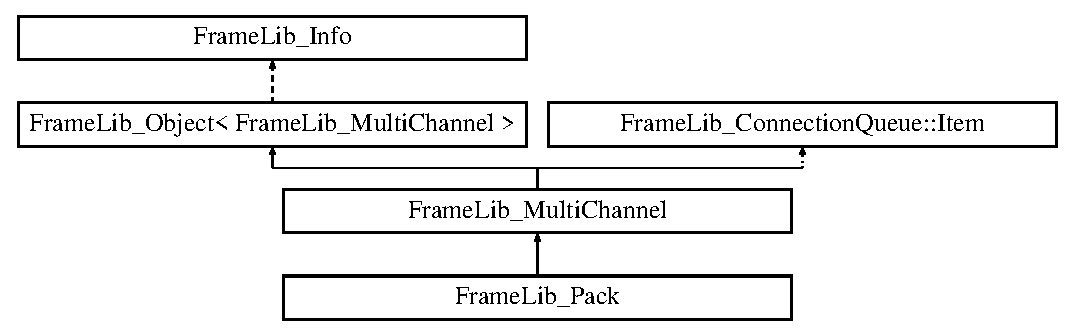
\includegraphics[height=4.000000cm]{class_frame_lib___pack}
\end{center}
\end{figure}
\subsection*{Public Member Functions}
\begin{DoxyCompactItemize}
\item 
\hyperlink{class_frame_lib___pack_aded2a9815261f73a8231f5df6c647ac2}{Frame\+Lib\+\_\+\+Pack} (\hyperlink{class_frame_lib___context}{Frame\+Lib\+\_\+\+Context} context, \hyperlink{class_frame_lib___parameters_1_1_serial}{Frame\+Lib\+\_\+\+Parameters\+::\+Serial} $\ast$serialised\+Parameters, void $\ast$owner)
\item 
virtual std\+::string \hyperlink{class_frame_lib___pack_aa15c5f54847d99c3bd3f9c2cf7688fd2}{object\+Info} (bool verbose)
\item 
virtual std\+::string \hyperlink{class_frame_lib___pack_ae9dacf16825332c2227cd9fd9af9db1d}{input\+Info} (unsigned long idx, bool verbose)
\item 
virtual std\+::string \hyperlink{class_frame_lib___pack_a40e71debefbc3e5e507e4f494e9efd68}{output\+Info} (unsigned long idx, bool verbose)
\item 
virtual const \hyperlink{class_frame_lib___parameters}{Frame\+Lib\+\_\+\+Parameters} $\ast$ \hyperlink{class_frame_lib___pack_af3f27c6065dc2e5c8106de50c42d63c3}{get\+Parameters} () const
\item 
virtual \hyperlink{_frame_lib___types_8h_ad495a9f61af7fff07d7e97979d1ab854}{Frame\+Type} \hyperlink{class_frame_lib___pack_af516c48cb7d0e685c6572dbdd1377b66}{input\+Type} (unsigned long idx) const
\item 
virtual \hyperlink{_frame_lib___types_8h_ad495a9f61af7fff07d7e97979d1ab854}{Frame\+Type} \hyperlink{class_frame_lib___pack_a48e9118d038396653928116b5c69077f}{output\+Type} (unsigned long idx) const
\item 
virtual void \hyperlink{class_frame_lib___pack_aacf276d3ed114e4aa03b8e640164d116}{auto\+Ordering\+Connections} ()
\item 
virtual void \hyperlink{class_frame_lib___pack_af0b40307726462df7754ead87c7c8a9c}{clear\+Auto\+Ordering\+Connections} ()
\end{DoxyCompactItemize}
\subsection*{Additional Inherited Members}


\subsection{Constructor \& Destructor Documentation}
\mbox{\Hypertarget{class_frame_lib___pack_aded2a9815261f73a8231f5df6c647ac2}\label{class_frame_lib___pack_aded2a9815261f73a8231f5df6c647ac2}} 
\index{Frame\+Lib\+\_\+\+Pack@{Frame\+Lib\+\_\+\+Pack}!Frame\+Lib\+\_\+\+Pack@{Frame\+Lib\+\_\+\+Pack}}
\index{Frame\+Lib\+\_\+\+Pack@{Frame\+Lib\+\_\+\+Pack}!Frame\+Lib\+\_\+\+Pack@{Frame\+Lib\+\_\+\+Pack}}
\subsubsection{\texorpdfstring{Frame\+Lib\+\_\+\+Pack()}{FrameLib\_Pack()}}
{\footnotesize\ttfamily Frame\+Lib\+\_\+\+Pack\+::\+Frame\+Lib\+\_\+\+Pack (\begin{DoxyParamCaption}\item[{\hyperlink{class_frame_lib___context}{Frame\+Lib\+\_\+\+Context}}]{context,  }\item[{\hyperlink{class_frame_lib___parameters_1_1_serial}{Frame\+Lib\+\_\+\+Parameters\+::\+Serial} $\ast$}]{serialised\+Parameters,  }\item[{void $\ast$}]{owner }\end{DoxyParamCaption})}



\subsection{Member Function Documentation}
\mbox{\Hypertarget{class_frame_lib___pack_aacf276d3ed114e4aa03b8e640164d116}\label{class_frame_lib___pack_aacf276d3ed114e4aa03b8e640164d116}} 
\index{Frame\+Lib\+\_\+\+Pack@{Frame\+Lib\+\_\+\+Pack}!auto\+Ordering\+Connections@{auto\+Ordering\+Connections}}
\index{auto\+Ordering\+Connections@{auto\+Ordering\+Connections}!Frame\+Lib\+\_\+\+Pack@{Frame\+Lib\+\_\+\+Pack}}
\subsubsection{\texorpdfstring{auto\+Ordering\+Connections()}{autoOrderingConnections()}}
{\footnotesize\ttfamily virtual void Frame\+Lib\+\_\+\+Pack\+::auto\+Ordering\+Connections (\begin{DoxyParamCaption}{ }\end{DoxyParamCaption})\hspace{0.3cm}{\ttfamily [inline]}, {\ttfamily [virtual]}}



Implements \hyperlink{class_frame_lib___object_afa5bb93302a641c23b5eac7ab0dfe516}{Frame\+Lib\+\_\+\+Object$<$ Frame\+Lib\+\_\+\+Multi\+Channel $>$}.

\mbox{\Hypertarget{class_frame_lib___pack_af0b40307726462df7754ead87c7c8a9c}\label{class_frame_lib___pack_af0b40307726462df7754ead87c7c8a9c}} 
\index{Frame\+Lib\+\_\+\+Pack@{Frame\+Lib\+\_\+\+Pack}!clear\+Auto\+Ordering\+Connections@{clear\+Auto\+Ordering\+Connections}}
\index{clear\+Auto\+Ordering\+Connections@{clear\+Auto\+Ordering\+Connections}!Frame\+Lib\+\_\+\+Pack@{Frame\+Lib\+\_\+\+Pack}}
\subsubsection{\texorpdfstring{clear\+Auto\+Ordering\+Connections()}{clearAutoOrderingConnections()}}
{\footnotesize\ttfamily virtual void Frame\+Lib\+\_\+\+Pack\+::clear\+Auto\+Ordering\+Connections (\begin{DoxyParamCaption}{ }\end{DoxyParamCaption})\hspace{0.3cm}{\ttfamily [inline]}, {\ttfamily [virtual]}}



Implements \hyperlink{class_frame_lib___object_aac43ebfacb59081f7f60957380df7481}{Frame\+Lib\+\_\+\+Object$<$ Frame\+Lib\+\_\+\+Multi\+Channel $>$}.

\mbox{\Hypertarget{class_frame_lib___pack_af3f27c6065dc2e5c8106de50c42d63c3}\label{class_frame_lib___pack_af3f27c6065dc2e5c8106de50c42d63c3}} 
\index{Frame\+Lib\+\_\+\+Pack@{Frame\+Lib\+\_\+\+Pack}!get\+Parameters@{get\+Parameters}}
\index{get\+Parameters@{get\+Parameters}!Frame\+Lib\+\_\+\+Pack@{Frame\+Lib\+\_\+\+Pack}}
\subsubsection{\texorpdfstring{get\+Parameters()}{getParameters()}}
{\footnotesize\ttfamily virtual const \hyperlink{class_frame_lib___parameters}{Frame\+Lib\+\_\+\+Parameters}$\ast$ Frame\+Lib\+\_\+\+Pack\+::get\+Parameters (\begin{DoxyParamCaption}{ }\end{DoxyParamCaption}) const\hspace{0.3cm}{\ttfamily [inline]}, {\ttfamily [virtual]}}



Reimplemented from \hyperlink{class_frame_lib___object_ac90a6770aeef26ee1601889dc16dba56}{Frame\+Lib\+\_\+\+Object$<$ Frame\+Lib\+\_\+\+Multi\+Channel $>$}.

\mbox{\Hypertarget{class_frame_lib___pack_ae9dacf16825332c2227cd9fd9af9db1d}\label{class_frame_lib___pack_ae9dacf16825332c2227cd9fd9af9db1d}} 
\index{Frame\+Lib\+\_\+\+Pack@{Frame\+Lib\+\_\+\+Pack}!input\+Info@{input\+Info}}
\index{input\+Info@{input\+Info}!Frame\+Lib\+\_\+\+Pack@{Frame\+Lib\+\_\+\+Pack}}
\subsubsection{\texorpdfstring{input\+Info()}{inputInfo()}}
{\footnotesize\ttfamily std\+::string Frame\+Lib\+\_\+\+Pack\+::input\+Info (\begin{DoxyParamCaption}\item[{unsigned long}]{idx,  }\item[{bool}]{verbose }\end{DoxyParamCaption})\hspace{0.3cm}{\ttfamily [virtual]}}



Reimplemented from \hyperlink{class_frame_lib___object_a49abea5f18125c425b1eae8710735891}{Frame\+Lib\+\_\+\+Object$<$ Frame\+Lib\+\_\+\+Multi\+Channel $>$}.

\mbox{\Hypertarget{class_frame_lib___pack_af516c48cb7d0e685c6572dbdd1377b66}\label{class_frame_lib___pack_af516c48cb7d0e685c6572dbdd1377b66}} 
\index{Frame\+Lib\+\_\+\+Pack@{Frame\+Lib\+\_\+\+Pack}!input\+Type@{input\+Type}}
\index{input\+Type@{input\+Type}!Frame\+Lib\+\_\+\+Pack@{Frame\+Lib\+\_\+\+Pack}}
\subsubsection{\texorpdfstring{input\+Type()}{inputType()}}
{\footnotesize\ttfamily virtual \hyperlink{_frame_lib___types_8h_ad495a9f61af7fff07d7e97979d1ab854}{Frame\+Type} Frame\+Lib\+\_\+\+Pack\+::input\+Type (\begin{DoxyParamCaption}\item[{unsigned long}]{idx }\end{DoxyParamCaption}) const\hspace{0.3cm}{\ttfamily [inline]}, {\ttfamily [virtual]}}



Implements \hyperlink{class_frame_lib___object_ab1ab1ae8180bb8b7e881aac6a4e1066c}{Frame\+Lib\+\_\+\+Object$<$ Frame\+Lib\+\_\+\+Multi\+Channel $>$}.

\mbox{\Hypertarget{class_frame_lib___pack_aa15c5f54847d99c3bd3f9c2cf7688fd2}\label{class_frame_lib___pack_aa15c5f54847d99c3bd3f9c2cf7688fd2}} 
\index{Frame\+Lib\+\_\+\+Pack@{Frame\+Lib\+\_\+\+Pack}!object\+Info@{object\+Info}}
\index{object\+Info@{object\+Info}!Frame\+Lib\+\_\+\+Pack@{Frame\+Lib\+\_\+\+Pack}}
\subsubsection{\texorpdfstring{object\+Info()}{objectInfo()}}
{\footnotesize\ttfamily std\+::string Frame\+Lib\+\_\+\+Pack\+::object\+Info (\begin{DoxyParamCaption}\item[{bool}]{verbose }\end{DoxyParamCaption})\hspace{0.3cm}{\ttfamily [virtual]}}



Reimplemented from \hyperlink{class_frame_lib___object_a10d673de9a3c59ace6a22ba1cff313c8}{Frame\+Lib\+\_\+\+Object$<$ Frame\+Lib\+\_\+\+Multi\+Channel $>$}.

\mbox{\Hypertarget{class_frame_lib___pack_a40e71debefbc3e5e507e4f494e9efd68}\label{class_frame_lib___pack_a40e71debefbc3e5e507e4f494e9efd68}} 
\index{Frame\+Lib\+\_\+\+Pack@{Frame\+Lib\+\_\+\+Pack}!output\+Info@{output\+Info}}
\index{output\+Info@{output\+Info}!Frame\+Lib\+\_\+\+Pack@{Frame\+Lib\+\_\+\+Pack}}
\subsubsection{\texorpdfstring{output\+Info()}{outputInfo()}}
{\footnotesize\ttfamily std\+::string Frame\+Lib\+\_\+\+Pack\+::output\+Info (\begin{DoxyParamCaption}\item[{unsigned long}]{idx,  }\item[{bool}]{verbose }\end{DoxyParamCaption})\hspace{0.3cm}{\ttfamily [virtual]}}



Reimplemented from \hyperlink{class_frame_lib___object_a6e6d79e8d620eedbaa50abf324cdedf5}{Frame\+Lib\+\_\+\+Object$<$ Frame\+Lib\+\_\+\+Multi\+Channel $>$}.

\mbox{\Hypertarget{class_frame_lib___pack_a48e9118d038396653928116b5c69077f}\label{class_frame_lib___pack_a48e9118d038396653928116b5c69077f}} 
\index{Frame\+Lib\+\_\+\+Pack@{Frame\+Lib\+\_\+\+Pack}!output\+Type@{output\+Type}}
\index{output\+Type@{output\+Type}!Frame\+Lib\+\_\+\+Pack@{Frame\+Lib\+\_\+\+Pack}}
\subsubsection{\texorpdfstring{output\+Type()}{outputType()}}
{\footnotesize\ttfamily virtual \hyperlink{_frame_lib___types_8h_ad495a9f61af7fff07d7e97979d1ab854}{Frame\+Type} Frame\+Lib\+\_\+\+Pack\+::output\+Type (\begin{DoxyParamCaption}\item[{unsigned long}]{idx }\end{DoxyParamCaption}) const\hspace{0.3cm}{\ttfamily [inline]}, {\ttfamily [virtual]}}



Implements \hyperlink{class_frame_lib___object_a03eb408844f15d8f73cee67f43149b9d}{Frame\+Lib\+\_\+\+Object$<$ Frame\+Lib\+\_\+\+Multi\+Channel $>$}.



The documentation for this class was generated from the following files\+:\begin{DoxyCompactItemize}
\item 
/\+Users/alexharker/\+Documents/\+Max Externals/\+Frame\+Lib/\+Frame\+Lib\+\_\+\+Framework/\hyperlink{_frame_lib___multichannel_8h}{Frame\+Lib\+\_\+\+Multichannel.\+h}\item 
/\+Users/alexharker/\+Documents/\+Max Externals/\+Frame\+Lib/\+Frame\+Lib\+\_\+\+Framework/\hyperlink{_frame_lib___multichannel_8cpp}{Frame\+Lib\+\_\+\+Multichannel.\+cpp}\end{DoxyCompactItemize}

\hypertarget{class_frame_lib___parameters}{}\section{Frame\+Lib\+\_\+\+Parameters Class Reference}
\label{class_frame_lib___parameters}\index{Frame\+Lib\+\_\+\+Parameters@{Frame\+Lib\+\_\+\+Parameters}}


{\ttfamily \#include $<$Frame\+Lib\+\_\+\+Parameters.\+h$>$}

\subsection*{Classes}
\begin{DoxyCompactItemize}
\item 
class \hyperlink{class_frame_lib___parameters_1_1_auto_serial}{Auto\+Serial}
\item 
class \hyperlink{class_frame_lib___parameters_1_1_info}{Info}
\item 
class \hyperlink{class_frame_lib___parameters_1_1_serial}{Serial}
\end{DoxyCompactItemize}
\subsection*{Public Types}
\begin{DoxyCompactItemize}
\item 
enum \hyperlink{class_frame_lib___parameters_a61fa243341eccefa66dbb744b7e047a0}{Numeric\+Type} \{ \hyperlink{class_frame_lib___parameters_a61fa243341eccefa66dbb744b7e047a0a276b662bb47e28e71aa9374b2c9583df}{k\+Numeric\+Bool}, 
\hyperlink{class_frame_lib___parameters_a61fa243341eccefa66dbb744b7e047a0af4eb00dbe8016ef96f31092df714d02e}{k\+Numeric\+Integer}, 
\hyperlink{class_frame_lib___parameters_a61fa243341eccefa66dbb744b7e047a0ac3c5ba5da1109012d2351911622767ee}{k\+Numeric\+Double}, 
\hyperlink{class_frame_lib___parameters_a61fa243341eccefa66dbb744b7e047a0ac4ef7b3184143f6cf48ba5aacf4afe15}{k\+Numeric\+None}
 \}
\item 
enum \hyperlink{class_frame_lib___parameters_a01bd45aaa25fa8cfaec369e2c8a8371a}{Type} \{ \newline
\hyperlink{class_frame_lib___parameters_a01bd45aaa25fa8cfaec369e2c8a8371aa43cf5c8a114a76cac0e943b3c9629b4b}{k\+Value}, 
\hyperlink{class_frame_lib___parameters_a01bd45aaa25fa8cfaec369e2c8a8371aae4be9c3bbdbe55e5e3dbb6c0d137c55f}{k\+Enum}, 
\hyperlink{class_frame_lib___parameters_a01bd45aaa25fa8cfaec369e2c8a8371aa827654e4ba3c421c522ec9d3bf2fc53f}{k\+String}, 
\hyperlink{class_frame_lib___parameters_a01bd45aaa25fa8cfaec369e2c8a8371aa7b2efcbcd57063e0b8c79db30ee60c74}{k\+Array}, 
\newline
\hyperlink{class_frame_lib___parameters_a01bd45aaa25fa8cfaec369e2c8a8371aa03c56a5d94eda74df98b245ebb2def2b}{k\+Variable\+Array}
 \}
\item 
enum \hyperlink{class_frame_lib___parameters_afcefd8a6a664599b93f635538d95265a}{Clip\+Mode} \{ \hyperlink{class_frame_lib___parameters_afcefd8a6a664599b93f635538d95265aa74d385df6b21c2f8fe20454725b41b08}{k\+None}, 
\hyperlink{class_frame_lib___parameters_afcefd8a6a664599b93f635538d95265aaba937501eab62c28a9c6be9f80647924}{k\+Min}, 
\hyperlink{class_frame_lib___parameters_afcefd8a6a664599b93f635538d95265aab9b24c826e2734c4ab24c242f22c0c7d}{k\+Max}, 
\hyperlink{class_frame_lib___parameters_afcefd8a6a664599b93f635538d95265aad36dffe61b1814eb301e184c88cfed0a}{k\+Clip}
 \}
\end{DoxyCompactItemize}
\subsection*{Public Member Functions}
\begin{DoxyCompactItemize}
\item 
\hyperlink{class_frame_lib___parameters_a901d16f8654b147d21cf2b87d3ed8a14}{Frame\+Lib\+\_\+\+Parameters} (\hyperlink{class_frame_lib___parameters_1_1_info}{Info} $\ast$info)
\item 
\hyperlink{class_frame_lib___parameters_a5bb469337e8a213ba9f397bc6af269c8}{$\sim$\+Frame\+Lib\+\_\+\+Parameters} ()
\item 
unsigned long \hyperlink{class_frame_lib___parameters_a391d0cb37c904981f7ad52bc0ba1b111}{size} () const
\item 
long \hyperlink{class_frame_lib___parameters_a6188f2b27de6850129ea084c99aa4669}{get\+Idx} (const char $\ast$name) const
\item 
long \hyperlink{class_frame_lib___parameters_a79b95cc8a0494356b12fa2ac51ece583}{max\+Argument} () const
\item 
void \hyperlink{class_frame_lib___parameters_ad975cc435f4fa2006e1a722dad784d9a}{add\+Bool} (unsigned long index, const char $\ast$name, bool default\+Value=false, long argument\+Idx=-\/1)
\item 
void \hyperlink{class_frame_lib___parameters_ab05bf4cd30eecd26bba972efd171798c}{add\+Double} (unsigned long index, const char $\ast$name, double default\+Value=0.\+0, long argument\+Idx=-\/1)
\item 
void \hyperlink{class_frame_lib___parameters_a9cb86d9fa829686a58e7776dcc45b60a}{add\+Int} (unsigned long index, const char $\ast$name, long default\+Value=0, long argument\+Idx=-\/1)
\item 
void \hyperlink{class_frame_lib___parameters_a54881a00c48e949914b130383c110a0a}{add\+String} (unsigned long index, const char $\ast$name, long argument\+Idx=-\/1)
\item 
void \hyperlink{class_frame_lib___parameters_ae79973b1261a0a63a14f6c4b299d0fb6}{add\+Enum} (unsigned long index, const char $\ast$name, long argument\+Idx=-\/1)
\item 
void \hyperlink{class_frame_lib___parameters_a9840a17de7f4c3078d26f23ec88eb02d}{add\+Enum\+Item} (unsigned long index, const char $\ast$str)
\item 
void \hyperlink{class_frame_lib___parameters_a9239184fd366b1cbaeec545577c20ab2}{add\+Bool\+Array} (unsigned long index, const char $\ast$name, long default\+Value, size\+\_\+t \hyperlink{class_frame_lib___parameters_a391d0cb37c904981f7ad52bc0ba1b111}{size}, long argument\+Idx=-\/1)
\item 
void \hyperlink{class_frame_lib___parameters_a409ad961a1376b59eb9927894ee08d35}{add\+Int\+Array} (unsigned long index, const char $\ast$name, long default\+Value, size\+\_\+t \hyperlink{class_frame_lib___parameters_a391d0cb37c904981f7ad52bc0ba1b111}{size}, long argument\+Idx=-\/1)
\item 
void \hyperlink{class_frame_lib___parameters_adfdb57e149f9c14afabf37a39263ad16}{add\+Double\+Array} (unsigned long index, const char $\ast$name, double default\+Value, size\+\_\+t \hyperlink{class_frame_lib___parameters_a391d0cb37c904981f7ad52bc0ba1b111}{size}, long argument\+Idx=-\/1)
\item 
void \hyperlink{class_frame_lib___parameters_a7d29ce5a989b58dd19a00fccea66de9f}{add\+Variable\+Bool\+Array} (unsigned long index, const char $\ast$name, long default\+Value, size\+\_\+t max\+Size, size\+\_\+t \hyperlink{class_frame_lib___parameters_a391d0cb37c904981f7ad52bc0ba1b111}{size}, long argument\+Idx=-\/1)
\item 
void \hyperlink{class_frame_lib___parameters_abd0359eb3df2b07acf25ef5d1f2873fe}{add\+Variable\+Int\+Array} (unsigned long index, const char $\ast$name, long default\+Value, size\+\_\+t max\+Size, size\+\_\+t \hyperlink{class_frame_lib___parameters_a391d0cb37c904981f7ad52bc0ba1b111}{size}, long argument\+Idx=-\/1)
\item 
void \hyperlink{class_frame_lib___parameters_afefc06df8236e718674b7d7adac313ec}{add\+Variable\+Double\+Array} (unsigned long index, const char $\ast$name, double default\+Value, size\+\_\+t max\+Size, size\+\_\+t \hyperlink{class_frame_lib___parameters_a391d0cb37c904981f7ad52bc0ba1b111}{size}, long argument\+Idx=-\/1)
\item 
void \hyperlink{class_frame_lib___parameters_a29ca4962b55f16a90fd54a246fb17810}{set\+Instantiation} ()
\item 
void \hyperlink{class_frame_lib___parameters_ad3ade0db8b31a6cc85f4b66b6ad94cca}{set\+Min} (double min)
\item 
void \hyperlink{class_frame_lib___parameters_a921441264480d6e01d6053c21d98a8f8}{set\+Max} (double max)
\item 
void \hyperlink{class_frame_lib___parameters_aadd3ae63aa5ea79bc65f16bc892522e3}{set\+Clip} (double min, double max)
\item 
void \hyperlink{class_frame_lib___parameters_a1028e3913b7f38000f71ce4b172143a7}{set} (\hyperlink{class_frame_lib___parameters_1_1_serial}{Serial} $\ast$serialised)
\item 
void \hyperlink{class_frame_lib___parameters_ac6f06219212d719bdbebfd71ef8af498}{set} (unsigned long idx, bool value)
\item 
void \hyperlink{class_frame_lib___parameters_a9dad319808446724cecb563e73468f44}{set} (const char $\ast$name, bool value)
\item 
void \hyperlink{class_frame_lib___parameters_a84c1cba168d37877b3883302af6c3d9e}{set} (unsigned long idx, long value)
\item 
void \hyperlink{class_frame_lib___parameters_abf85c9c040394d99956bd46b0227b3c7}{set} (const char $\ast$name, long value)
\item 
void \hyperlink{class_frame_lib___parameters_a0391ec487908f254507df22ad88e8745}{set} (unsigned long idx, double value)
\item 
void \hyperlink{class_frame_lib___parameters_a6b1af7f2835bd529388055fac19ba494}{set} (const char $\ast$name, double value)
\item 
void \hyperlink{class_frame_lib___parameters_a076802f4d9ac90035a4202c5acb7333f}{set} (unsigned long idx, char $\ast$str)
\item 
void \hyperlink{class_frame_lib___parameters_aaa0b5e9c31955ba649e69ba8971dbe5d}{set} (const char $\ast$name, char $\ast$str)
\item 
void \hyperlink{class_frame_lib___parameters_a2cd3483982c6b856744bdd8782b2f522}{set} (unsigned long idx, double $\ast$values, size\+\_\+t N)
\item 
void \hyperlink{class_frame_lib___parameters_add616cf6328c08d81d1af54ff6109059}{set} (const char $\ast$name, double $\ast$values, size\+\_\+t N)
\item 
void \hyperlink{class_frame_lib___parameters_a5c0764e11e7723b034fc9951b4dcfb3e}{clear} (unsigned long idx)
\item 
void \hyperlink{class_frame_lib___parameters_a6a4c25214fbf10b639346170c957d3f5}{clear} (const char $\ast$name)
\item 
std\+::string \hyperlink{class_frame_lib___parameters_a525cfe083e686bc5de04aee1004f3bfe}{get\+Name} (unsigned long idx) const
\item 
long \hyperlink{class_frame_lib___parameters_a9dd267fcd72252b366d7f0fd5112e668}{get\+Argument\+Idx} (unsigned long idx) const
\item 
long \hyperlink{class_frame_lib___parameters_a91ad76185df1c37e58f18cb7fc81c140}{get\+Argument\+Idx} (const char $\ast$name) const
\item 
\hyperlink{class_frame_lib___parameters_a01bd45aaa25fa8cfaec369e2c8a8371a}{Type} \hyperlink{class_frame_lib___parameters_ae81f3bf43c6301b1abadd5b2539f8925}{get\+Type} (unsigned long idx) const
\item 
\hyperlink{class_frame_lib___parameters_a01bd45aaa25fa8cfaec369e2c8a8371a}{Type} \hyperlink{class_frame_lib___parameters_a705bba592b790d1b884b2ea4dd4bdbd4}{get\+Type} (const char $\ast$name) const
\item 
\hyperlink{class_frame_lib___parameters_a61fa243341eccefa66dbb744b7e047a0}{Numeric\+Type} \hyperlink{class_frame_lib___parameters_a57052803e8a3ab34c40bf4dedd33e196}{get\+Numeric\+Type} (unsigned long idx) const
\item 
\hyperlink{class_frame_lib___parameters_a61fa243341eccefa66dbb744b7e047a0}{Numeric\+Type} \hyperlink{class_frame_lib___parameters_a7d9b774329a6e87643a6714913687cfe}{get\+Numeric\+Type} (const char $\ast$name) const
\item 
std\+::string \hyperlink{class_frame_lib___parameters_a75457679ab4b67d5d438bf8619544d94}{get\+Type\+String} (unsigned long idx) const
\item 
std\+::string \hyperlink{class_frame_lib___parameters_a7531a5e8e9ea19a84dd8314ed2ebe4f3}{get\+Type\+String} (const char $\ast$name) const
\item 
\hyperlink{class_frame_lib___parameters_afcefd8a6a664599b93f635538d95265a}{Clip\+Mode} \hyperlink{class_frame_lib___parameters_ac574f7fd7e17b4d5df393c84b81b4431}{get\+Clip\+Mode} (unsigned long idx) const
\item 
\hyperlink{class_frame_lib___parameters_afcefd8a6a664599b93f635538d95265a}{Clip\+Mode} \hyperlink{class_frame_lib___parameters_ab54fc0edf6fed7029dec5dd09f884b38}{get\+Clip\+Mode} (const char $\ast$name) const
\item 
double \hyperlink{class_frame_lib___parameters_af73a52dd8beadde0c65159fd2d8d35ce}{get\+Min} (unsigned long idx) const
\item 
double \hyperlink{class_frame_lib___parameters_ac188e94ada437c42fceac7f1c502c536}{get\+Min} (const char $\ast$name) const
\item 
double \hyperlink{class_frame_lib___parameters_a6d18778368a98852e2d710748ecea5fb}{get\+Max} (unsigned long idx) const
\item 
double \hyperlink{class_frame_lib___parameters_a9b1b814d8df6fed63adb0854383df279}{get\+Max} (const char $\ast$name) const
\item 
void \hyperlink{class_frame_lib___parameters_a9addab9977edd69cc6cfa7b5f4a70a9d}{get\+Range} (unsigned long idx, double $\ast$min, double $\ast$max) const
\item 
void \hyperlink{class_frame_lib___parameters_a3287eb6847370554758129162e5eff11}{get\+Range} (const char $\ast$name, double $\ast$min, double $\ast$max) const
\item 
std\+::string \hyperlink{class_frame_lib___parameters_a19f6d2862f0b6c2a9fffa496362beef1}{get\+Item\+String} (unsigned long idx, unsigned long item) const
\item 
std\+::string \hyperlink{class_frame_lib___parameters_a5cda6528deb6a8a306b6de6f7eeaa2fb}{get\+Item\+String} (const char $\ast$name, unsigned long item) const
\item 
std\+::string \hyperlink{class_frame_lib___parameters_a6e90c72b4f3ece2ab4fe7dd893d399e3}{get\+Info} (unsigned long idx) const
\item 
std\+::string \hyperlink{class_frame_lib___parameters_aa278b4f3ac4bb743e2941fd004748133}{get\+Info} (const char $\ast$name) const
\item 
double \hyperlink{class_frame_lib___parameters_a6d28eb24ae285237724b2249f342c3d8}{get\+Default} (unsigned long idx) const
\item 
double \hyperlink{class_frame_lib___parameters_a2524dc5f2566eb521f95a342eb980239}{get\+Default} (const char $\ast$name) const
\item 
std\+::string \hyperlink{class_frame_lib___parameters_aa6544b983343464c17299ab6f1874bce}{get\+Default\+String} (unsigned long idx) const
\item 
std\+::string \hyperlink{class_frame_lib___parameters_aa8481b077e92ff7548123b97411280a1}{get\+Default\+String} (const char $\ast$name) const
\item 
double \hyperlink{class_frame_lib___parameters_a64dc41237eccad96a857b4f675f4054d}{get\+Value} (unsigned long idx) const
\item 
double \hyperlink{class_frame_lib___parameters_afa54042c7a35164482fcba5112bd3e24}{get\+Value} (const char $\ast$name) const
\item 
long \hyperlink{class_frame_lib___parameters_adc9dcbcbf2ac23f0e15a35db8090aa88}{get\+Int} (unsigned long idx) const
\item 
long \hyperlink{class_frame_lib___parameters_a31833d0ce833197dbde6346159bf3222}{get\+Int} (const char $\ast$name) const
\item 
long \hyperlink{class_frame_lib___parameters_ad27a46c31a31f42a6efb7c29c6937595}{get\+Bool} (unsigned long idx) const
\item 
bool \hyperlink{class_frame_lib___parameters_adb0e6fa234026a2cd72eb5baed059b30}{get\+Bool} (const char $\ast$name) const
\item 
const char $\ast$ \hyperlink{class_frame_lib___parameters_a9853e712e3ee11410175d6e3028d862a}{get\+String} (unsigned long idx) const
\item 
const char $\ast$ \hyperlink{class_frame_lib___parameters_acee2bbf4822572b7b37447462f50c44b}{get\+String} (const char $\ast$name) const
\item 
const double $\ast$ \hyperlink{class_frame_lib___parameters_adc277fde0bbaa9250076b58efc9428e6}{get\+Array} (unsigned long idx) const
\item 
const double $\ast$ \hyperlink{class_frame_lib___parameters_a4a5ff203e9384ca2fb73b7589a6de74e}{get\+Array} (const char $\ast$name) const
\item 
const double $\ast$ \hyperlink{class_frame_lib___parameters_a645085b04512fadc95ff59b910954bdc}{get\+Array} (unsigned long idx, size\+\_\+t $\ast$\hyperlink{class_frame_lib___parameters_a391d0cb37c904981f7ad52bc0ba1b111}{size}) const
\item 
const double $\ast$ \hyperlink{class_frame_lib___parameters_a09126c9d1be171bde88fe171944bc038}{get\+Array} (const char $\ast$name, size\+\_\+t $\ast$\hyperlink{class_frame_lib___parameters_a391d0cb37c904981f7ad52bc0ba1b111}{size}) const
\item 
size\+\_\+t \hyperlink{class_frame_lib___parameters_a393371aad3079281d84150f9343b8e88}{get\+Array\+Size} (unsigned long idx) const
\item 
size\+\_\+t \hyperlink{class_frame_lib___parameters_a6aab87bc340522a457d3275728d6ad69}{get\+Array\+Size} (const char $\ast$name) const
\item 
size\+\_\+t \hyperlink{class_frame_lib___parameters_ac65d6b2f5cee3b3c95b321c67de6fadb}{get\+Array\+Max\+Size} (unsigned long idx) const
\item 
size\+\_\+t \hyperlink{class_frame_lib___parameters_aa471582edb55bbb44146a560228821ef}{get\+Array\+Max\+Size} (const char $\ast$name) const
\item 
bool \hyperlink{class_frame_lib___parameters_a1ddc66de3c5b22c98c61692139d6edb1}{changed} (unsigned long idx)
\item 
bool \hyperlink{class_frame_lib___parameters_a6bd6af480a8d8f589ee7443c690f75b0}{changed} (const char $\ast$name)
\end{DoxyCompactItemize}


\subsection{Member Enumeration Documentation}
\mbox{\Hypertarget{class_frame_lib___parameters_afcefd8a6a664599b93f635538d95265a}\label{class_frame_lib___parameters_afcefd8a6a664599b93f635538d95265a}} 
\index{Frame\+Lib\+\_\+\+Parameters@{Frame\+Lib\+\_\+\+Parameters}!Clip\+Mode@{Clip\+Mode}}
\index{Clip\+Mode@{Clip\+Mode}!Frame\+Lib\+\_\+\+Parameters@{Frame\+Lib\+\_\+\+Parameters}}
\subsubsection{\texorpdfstring{Clip\+Mode}{ClipMode}}
{\footnotesize\ttfamily enum \hyperlink{class_frame_lib___parameters_afcefd8a6a664599b93f635538d95265a}{Frame\+Lib\+\_\+\+Parameters\+::\+Clip\+Mode}}

\begin{DoxyEnumFields}{Enumerator}
\raisebox{\heightof{T}}[0pt][0pt]{\index{k\+None@{k\+None}!Frame\+Lib\+\_\+\+Parameters@{Frame\+Lib\+\_\+\+Parameters}}\index{Frame\+Lib\+\_\+\+Parameters@{Frame\+Lib\+\_\+\+Parameters}!k\+None@{k\+None}}}\mbox{\Hypertarget{class_frame_lib___parameters_afcefd8a6a664599b93f635538d95265aa74d385df6b21c2f8fe20454725b41b08}\label{class_frame_lib___parameters_afcefd8a6a664599b93f635538d95265aa74d385df6b21c2f8fe20454725b41b08}} 
k\+None&\\
\hline

\raisebox{\heightof{T}}[0pt][0pt]{\index{k\+Min@{k\+Min}!Frame\+Lib\+\_\+\+Parameters@{Frame\+Lib\+\_\+\+Parameters}}\index{Frame\+Lib\+\_\+\+Parameters@{Frame\+Lib\+\_\+\+Parameters}!k\+Min@{k\+Min}}}\mbox{\Hypertarget{class_frame_lib___parameters_afcefd8a6a664599b93f635538d95265aaba937501eab62c28a9c6be9f80647924}\label{class_frame_lib___parameters_afcefd8a6a664599b93f635538d95265aaba937501eab62c28a9c6be9f80647924}} 
k\+Min&\\
\hline

\raisebox{\heightof{T}}[0pt][0pt]{\index{k\+Max@{k\+Max}!Frame\+Lib\+\_\+\+Parameters@{Frame\+Lib\+\_\+\+Parameters}}\index{Frame\+Lib\+\_\+\+Parameters@{Frame\+Lib\+\_\+\+Parameters}!k\+Max@{k\+Max}}}\mbox{\Hypertarget{class_frame_lib___parameters_afcefd8a6a664599b93f635538d95265aab9b24c826e2734c4ab24c242f22c0c7d}\label{class_frame_lib___parameters_afcefd8a6a664599b93f635538d95265aab9b24c826e2734c4ab24c242f22c0c7d}} 
k\+Max&\\
\hline

\raisebox{\heightof{T}}[0pt][0pt]{\index{k\+Clip@{k\+Clip}!Frame\+Lib\+\_\+\+Parameters@{Frame\+Lib\+\_\+\+Parameters}}\index{Frame\+Lib\+\_\+\+Parameters@{Frame\+Lib\+\_\+\+Parameters}!k\+Clip@{k\+Clip}}}\mbox{\Hypertarget{class_frame_lib___parameters_afcefd8a6a664599b93f635538d95265aad36dffe61b1814eb301e184c88cfed0a}\label{class_frame_lib___parameters_afcefd8a6a664599b93f635538d95265aad36dffe61b1814eb301e184c88cfed0a}} 
k\+Clip&\\
\hline

\end{DoxyEnumFields}
\mbox{\Hypertarget{class_frame_lib___parameters_a61fa243341eccefa66dbb744b7e047a0}\label{class_frame_lib___parameters_a61fa243341eccefa66dbb744b7e047a0}} 
\index{Frame\+Lib\+\_\+\+Parameters@{Frame\+Lib\+\_\+\+Parameters}!Numeric\+Type@{Numeric\+Type}}
\index{Numeric\+Type@{Numeric\+Type}!Frame\+Lib\+\_\+\+Parameters@{Frame\+Lib\+\_\+\+Parameters}}
\subsubsection{\texorpdfstring{Numeric\+Type}{NumericType}}
{\footnotesize\ttfamily enum \hyperlink{class_frame_lib___parameters_a61fa243341eccefa66dbb744b7e047a0}{Frame\+Lib\+\_\+\+Parameters\+::\+Numeric\+Type}}

\begin{DoxyEnumFields}{Enumerator}
\raisebox{\heightof{T}}[0pt][0pt]{\index{k\+Numeric\+Bool@{k\+Numeric\+Bool}!Frame\+Lib\+\_\+\+Parameters@{Frame\+Lib\+\_\+\+Parameters}}\index{Frame\+Lib\+\_\+\+Parameters@{Frame\+Lib\+\_\+\+Parameters}!k\+Numeric\+Bool@{k\+Numeric\+Bool}}}\mbox{\Hypertarget{class_frame_lib___parameters_a61fa243341eccefa66dbb744b7e047a0a276b662bb47e28e71aa9374b2c9583df}\label{class_frame_lib___parameters_a61fa243341eccefa66dbb744b7e047a0a276b662bb47e28e71aa9374b2c9583df}} 
k\+Numeric\+Bool&\\
\hline

\raisebox{\heightof{T}}[0pt][0pt]{\index{k\+Numeric\+Integer@{k\+Numeric\+Integer}!Frame\+Lib\+\_\+\+Parameters@{Frame\+Lib\+\_\+\+Parameters}}\index{Frame\+Lib\+\_\+\+Parameters@{Frame\+Lib\+\_\+\+Parameters}!k\+Numeric\+Integer@{k\+Numeric\+Integer}}}\mbox{\Hypertarget{class_frame_lib___parameters_a61fa243341eccefa66dbb744b7e047a0af4eb00dbe8016ef96f31092df714d02e}\label{class_frame_lib___parameters_a61fa243341eccefa66dbb744b7e047a0af4eb00dbe8016ef96f31092df714d02e}} 
k\+Numeric\+Integer&\\
\hline

\raisebox{\heightof{T}}[0pt][0pt]{\index{k\+Numeric\+Double@{k\+Numeric\+Double}!Frame\+Lib\+\_\+\+Parameters@{Frame\+Lib\+\_\+\+Parameters}}\index{Frame\+Lib\+\_\+\+Parameters@{Frame\+Lib\+\_\+\+Parameters}!k\+Numeric\+Double@{k\+Numeric\+Double}}}\mbox{\Hypertarget{class_frame_lib___parameters_a61fa243341eccefa66dbb744b7e047a0ac3c5ba5da1109012d2351911622767ee}\label{class_frame_lib___parameters_a61fa243341eccefa66dbb744b7e047a0ac3c5ba5da1109012d2351911622767ee}} 
k\+Numeric\+Double&\\
\hline

\raisebox{\heightof{T}}[0pt][0pt]{\index{k\+Numeric\+None@{k\+Numeric\+None}!Frame\+Lib\+\_\+\+Parameters@{Frame\+Lib\+\_\+\+Parameters}}\index{Frame\+Lib\+\_\+\+Parameters@{Frame\+Lib\+\_\+\+Parameters}!k\+Numeric\+None@{k\+Numeric\+None}}}\mbox{\Hypertarget{class_frame_lib___parameters_a61fa243341eccefa66dbb744b7e047a0ac4ef7b3184143f6cf48ba5aacf4afe15}\label{class_frame_lib___parameters_a61fa243341eccefa66dbb744b7e047a0ac4ef7b3184143f6cf48ba5aacf4afe15}} 
k\+Numeric\+None&\\
\hline

\end{DoxyEnumFields}
\mbox{\Hypertarget{class_frame_lib___parameters_a01bd45aaa25fa8cfaec369e2c8a8371a}\label{class_frame_lib___parameters_a01bd45aaa25fa8cfaec369e2c8a8371a}} 
\index{Frame\+Lib\+\_\+\+Parameters@{Frame\+Lib\+\_\+\+Parameters}!Type@{Type}}
\index{Type@{Type}!Frame\+Lib\+\_\+\+Parameters@{Frame\+Lib\+\_\+\+Parameters}}
\subsubsection{\texorpdfstring{Type}{Type}}
{\footnotesize\ttfamily enum \hyperlink{class_frame_lib___parameters_a01bd45aaa25fa8cfaec369e2c8a8371a}{Frame\+Lib\+\_\+\+Parameters\+::\+Type}}

\begin{DoxyEnumFields}{Enumerator}
\raisebox{\heightof{T}}[0pt][0pt]{\index{k\+Value@{k\+Value}!Frame\+Lib\+\_\+\+Parameters@{Frame\+Lib\+\_\+\+Parameters}}\index{Frame\+Lib\+\_\+\+Parameters@{Frame\+Lib\+\_\+\+Parameters}!k\+Value@{k\+Value}}}\mbox{\Hypertarget{class_frame_lib___parameters_a01bd45aaa25fa8cfaec369e2c8a8371aa43cf5c8a114a76cac0e943b3c9629b4b}\label{class_frame_lib___parameters_a01bd45aaa25fa8cfaec369e2c8a8371aa43cf5c8a114a76cac0e943b3c9629b4b}} 
k\+Value&\\
\hline

\raisebox{\heightof{T}}[0pt][0pt]{\index{k\+Enum@{k\+Enum}!Frame\+Lib\+\_\+\+Parameters@{Frame\+Lib\+\_\+\+Parameters}}\index{Frame\+Lib\+\_\+\+Parameters@{Frame\+Lib\+\_\+\+Parameters}!k\+Enum@{k\+Enum}}}\mbox{\Hypertarget{class_frame_lib___parameters_a01bd45aaa25fa8cfaec369e2c8a8371aae4be9c3bbdbe55e5e3dbb6c0d137c55f}\label{class_frame_lib___parameters_a01bd45aaa25fa8cfaec369e2c8a8371aae4be9c3bbdbe55e5e3dbb6c0d137c55f}} 
k\+Enum&\\
\hline

\raisebox{\heightof{T}}[0pt][0pt]{\index{k\+String@{k\+String}!Frame\+Lib\+\_\+\+Parameters@{Frame\+Lib\+\_\+\+Parameters}}\index{Frame\+Lib\+\_\+\+Parameters@{Frame\+Lib\+\_\+\+Parameters}!k\+String@{k\+String}}}\mbox{\Hypertarget{class_frame_lib___parameters_a01bd45aaa25fa8cfaec369e2c8a8371aa827654e4ba3c421c522ec9d3bf2fc53f}\label{class_frame_lib___parameters_a01bd45aaa25fa8cfaec369e2c8a8371aa827654e4ba3c421c522ec9d3bf2fc53f}} 
k\+String&\\
\hline

\raisebox{\heightof{T}}[0pt][0pt]{\index{k\+Array@{k\+Array}!Frame\+Lib\+\_\+\+Parameters@{Frame\+Lib\+\_\+\+Parameters}}\index{Frame\+Lib\+\_\+\+Parameters@{Frame\+Lib\+\_\+\+Parameters}!k\+Array@{k\+Array}}}\mbox{\Hypertarget{class_frame_lib___parameters_a01bd45aaa25fa8cfaec369e2c8a8371aa7b2efcbcd57063e0b8c79db30ee60c74}\label{class_frame_lib___parameters_a01bd45aaa25fa8cfaec369e2c8a8371aa7b2efcbcd57063e0b8c79db30ee60c74}} 
k\+Array&\\
\hline

\raisebox{\heightof{T}}[0pt][0pt]{\index{k\+Variable\+Array@{k\+Variable\+Array}!Frame\+Lib\+\_\+\+Parameters@{Frame\+Lib\+\_\+\+Parameters}}\index{Frame\+Lib\+\_\+\+Parameters@{Frame\+Lib\+\_\+\+Parameters}!k\+Variable\+Array@{k\+Variable\+Array}}}\mbox{\Hypertarget{class_frame_lib___parameters_a01bd45aaa25fa8cfaec369e2c8a8371aa03c56a5d94eda74df98b245ebb2def2b}\label{class_frame_lib___parameters_a01bd45aaa25fa8cfaec369e2c8a8371aa03c56a5d94eda74df98b245ebb2def2b}} 
k\+Variable\+Array&\\
\hline

\end{DoxyEnumFields}


\subsection{Constructor \& Destructor Documentation}
\mbox{\Hypertarget{class_frame_lib___parameters_a901d16f8654b147d21cf2b87d3ed8a14}\label{class_frame_lib___parameters_a901d16f8654b147d21cf2b87d3ed8a14}} 
\index{Frame\+Lib\+\_\+\+Parameters@{Frame\+Lib\+\_\+\+Parameters}!Frame\+Lib\+\_\+\+Parameters@{Frame\+Lib\+\_\+\+Parameters}}
\index{Frame\+Lib\+\_\+\+Parameters@{Frame\+Lib\+\_\+\+Parameters}!Frame\+Lib\+\_\+\+Parameters@{Frame\+Lib\+\_\+\+Parameters}}
\subsubsection{\texorpdfstring{Frame\+Lib\+\_\+\+Parameters()}{FrameLib\_Parameters()}}
{\footnotesize\ttfamily Frame\+Lib\+\_\+\+Parameters\+::\+Frame\+Lib\+\_\+\+Parameters (\begin{DoxyParamCaption}\item[{\hyperlink{class_frame_lib___parameters_1_1_info}{Info} $\ast$}]{info }\end{DoxyParamCaption})\hspace{0.3cm}{\ttfamily [inline]}}

\mbox{\Hypertarget{class_frame_lib___parameters_a5bb469337e8a213ba9f397bc6af269c8}\label{class_frame_lib___parameters_a5bb469337e8a213ba9f397bc6af269c8}} 
\index{Frame\+Lib\+\_\+\+Parameters@{Frame\+Lib\+\_\+\+Parameters}!````~Frame\+Lib\+\_\+\+Parameters@{$\sim$\+Frame\+Lib\+\_\+\+Parameters}}
\index{````~Frame\+Lib\+\_\+\+Parameters@{$\sim$\+Frame\+Lib\+\_\+\+Parameters}!Frame\+Lib\+\_\+\+Parameters@{Frame\+Lib\+\_\+\+Parameters}}
\subsubsection{\texorpdfstring{$\sim$\+Frame\+Lib\+\_\+\+Parameters()}{~FrameLib\_Parameters()}}
{\footnotesize\ttfamily Frame\+Lib\+\_\+\+Parameters\+::$\sim$\+Frame\+Lib\+\_\+\+Parameters (\begin{DoxyParamCaption}{ }\end{DoxyParamCaption})\hspace{0.3cm}{\ttfamily [inline]}}



\subsection{Member Function Documentation}
\mbox{\Hypertarget{class_frame_lib___parameters_ad975cc435f4fa2006e1a722dad784d9a}\label{class_frame_lib___parameters_ad975cc435f4fa2006e1a722dad784d9a}} 
\index{Frame\+Lib\+\_\+\+Parameters@{Frame\+Lib\+\_\+\+Parameters}!add\+Bool@{add\+Bool}}
\index{add\+Bool@{add\+Bool}!Frame\+Lib\+\_\+\+Parameters@{Frame\+Lib\+\_\+\+Parameters}}
\subsubsection{\texorpdfstring{add\+Bool()}{addBool()}}
{\footnotesize\ttfamily void Frame\+Lib\+\_\+\+Parameters\+::add\+Bool (\begin{DoxyParamCaption}\item[{unsigned long}]{index,  }\item[{const char $\ast$}]{name,  }\item[{bool}]{default\+Value = {\ttfamily false},  }\item[{long}]{argument\+Idx = {\ttfamily -\/1} }\end{DoxyParamCaption})\hspace{0.3cm}{\ttfamily [inline]}}

\mbox{\Hypertarget{class_frame_lib___parameters_a9239184fd366b1cbaeec545577c20ab2}\label{class_frame_lib___parameters_a9239184fd366b1cbaeec545577c20ab2}} 
\index{Frame\+Lib\+\_\+\+Parameters@{Frame\+Lib\+\_\+\+Parameters}!add\+Bool\+Array@{add\+Bool\+Array}}
\index{add\+Bool\+Array@{add\+Bool\+Array}!Frame\+Lib\+\_\+\+Parameters@{Frame\+Lib\+\_\+\+Parameters}}
\subsubsection{\texorpdfstring{add\+Bool\+Array()}{addBoolArray()}}
{\footnotesize\ttfamily void Frame\+Lib\+\_\+\+Parameters\+::add\+Bool\+Array (\begin{DoxyParamCaption}\item[{unsigned long}]{index,  }\item[{const char $\ast$}]{name,  }\item[{long}]{default\+Value,  }\item[{size\+\_\+t}]{size,  }\item[{long}]{argument\+Idx = {\ttfamily -\/1} }\end{DoxyParamCaption})\hspace{0.3cm}{\ttfamily [inline]}}

\mbox{\Hypertarget{class_frame_lib___parameters_ab05bf4cd30eecd26bba972efd171798c}\label{class_frame_lib___parameters_ab05bf4cd30eecd26bba972efd171798c}} 
\index{Frame\+Lib\+\_\+\+Parameters@{Frame\+Lib\+\_\+\+Parameters}!add\+Double@{add\+Double}}
\index{add\+Double@{add\+Double}!Frame\+Lib\+\_\+\+Parameters@{Frame\+Lib\+\_\+\+Parameters}}
\subsubsection{\texorpdfstring{add\+Double()}{addDouble()}}
{\footnotesize\ttfamily void Frame\+Lib\+\_\+\+Parameters\+::add\+Double (\begin{DoxyParamCaption}\item[{unsigned long}]{index,  }\item[{const char $\ast$}]{name,  }\item[{double}]{default\+Value = {\ttfamily 0.0},  }\item[{long}]{argument\+Idx = {\ttfamily -\/1} }\end{DoxyParamCaption})\hspace{0.3cm}{\ttfamily [inline]}}

\mbox{\Hypertarget{class_frame_lib___parameters_adfdb57e149f9c14afabf37a39263ad16}\label{class_frame_lib___parameters_adfdb57e149f9c14afabf37a39263ad16}} 
\index{Frame\+Lib\+\_\+\+Parameters@{Frame\+Lib\+\_\+\+Parameters}!add\+Double\+Array@{add\+Double\+Array}}
\index{add\+Double\+Array@{add\+Double\+Array}!Frame\+Lib\+\_\+\+Parameters@{Frame\+Lib\+\_\+\+Parameters}}
\subsubsection{\texorpdfstring{add\+Double\+Array()}{addDoubleArray()}}
{\footnotesize\ttfamily void Frame\+Lib\+\_\+\+Parameters\+::add\+Double\+Array (\begin{DoxyParamCaption}\item[{unsigned long}]{index,  }\item[{const char $\ast$}]{name,  }\item[{double}]{default\+Value,  }\item[{size\+\_\+t}]{size,  }\item[{long}]{argument\+Idx = {\ttfamily -\/1} }\end{DoxyParamCaption})\hspace{0.3cm}{\ttfamily [inline]}}

\mbox{\Hypertarget{class_frame_lib___parameters_ae79973b1261a0a63a14f6c4b299d0fb6}\label{class_frame_lib___parameters_ae79973b1261a0a63a14f6c4b299d0fb6}} 
\index{Frame\+Lib\+\_\+\+Parameters@{Frame\+Lib\+\_\+\+Parameters}!add\+Enum@{add\+Enum}}
\index{add\+Enum@{add\+Enum}!Frame\+Lib\+\_\+\+Parameters@{Frame\+Lib\+\_\+\+Parameters}}
\subsubsection{\texorpdfstring{add\+Enum()}{addEnum()}}
{\footnotesize\ttfamily void Frame\+Lib\+\_\+\+Parameters\+::add\+Enum (\begin{DoxyParamCaption}\item[{unsigned long}]{index,  }\item[{const char $\ast$}]{name,  }\item[{long}]{argument\+Idx = {\ttfamily -\/1} }\end{DoxyParamCaption})\hspace{0.3cm}{\ttfamily [inline]}}

\mbox{\Hypertarget{class_frame_lib___parameters_a9840a17de7f4c3078d26f23ec88eb02d}\label{class_frame_lib___parameters_a9840a17de7f4c3078d26f23ec88eb02d}} 
\index{Frame\+Lib\+\_\+\+Parameters@{Frame\+Lib\+\_\+\+Parameters}!add\+Enum\+Item@{add\+Enum\+Item}}
\index{add\+Enum\+Item@{add\+Enum\+Item}!Frame\+Lib\+\_\+\+Parameters@{Frame\+Lib\+\_\+\+Parameters}}
\subsubsection{\texorpdfstring{add\+Enum\+Item()}{addEnumItem()}}
{\footnotesize\ttfamily void Frame\+Lib\+\_\+\+Parameters\+::add\+Enum\+Item (\begin{DoxyParamCaption}\item[{unsigned long}]{index,  }\item[{const char $\ast$}]{str }\end{DoxyParamCaption})\hspace{0.3cm}{\ttfamily [inline]}}

\mbox{\Hypertarget{class_frame_lib___parameters_a9cb86d9fa829686a58e7776dcc45b60a}\label{class_frame_lib___parameters_a9cb86d9fa829686a58e7776dcc45b60a}} 
\index{Frame\+Lib\+\_\+\+Parameters@{Frame\+Lib\+\_\+\+Parameters}!add\+Int@{add\+Int}}
\index{add\+Int@{add\+Int}!Frame\+Lib\+\_\+\+Parameters@{Frame\+Lib\+\_\+\+Parameters}}
\subsubsection{\texorpdfstring{add\+Int()}{addInt()}}
{\footnotesize\ttfamily void Frame\+Lib\+\_\+\+Parameters\+::add\+Int (\begin{DoxyParamCaption}\item[{unsigned long}]{index,  }\item[{const char $\ast$}]{name,  }\item[{long}]{default\+Value = {\ttfamily 0},  }\item[{long}]{argument\+Idx = {\ttfamily -\/1} }\end{DoxyParamCaption})\hspace{0.3cm}{\ttfamily [inline]}}

\mbox{\Hypertarget{class_frame_lib___parameters_a409ad961a1376b59eb9927894ee08d35}\label{class_frame_lib___parameters_a409ad961a1376b59eb9927894ee08d35}} 
\index{Frame\+Lib\+\_\+\+Parameters@{Frame\+Lib\+\_\+\+Parameters}!add\+Int\+Array@{add\+Int\+Array}}
\index{add\+Int\+Array@{add\+Int\+Array}!Frame\+Lib\+\_\+\+Parameters@{Frame\+Lib\+\_\+\+Parameters}}
\subsubsection{\texorpdfstring{add\+Int\+Array()}{addIntArray()}}
{\footnotesize\ttfamily void Frame\+Lib\+\_\+\+Parameters\+::add\+Int\+Array (\begin{DoxyParamCaption}\item[{unsigned long}]{index,  }\item[{const char $\ast$}]{name,  }\item[{long}]{default\+Value,  }\item[{size\+\_\+t}]{size,  }\item[{long}]{argument\+Idx = {\ttfamily -\/1} }\end{DoxyParamCaption})\hspace{0.3cm}{\ttfamily [inline]}}

\mbox{\Hypertarget{class_frame_lib___parameters_a54881a00c48e949914b130383c110a0a}\label{class_frame_lib___parameters_a54881a00c48e949914b130383c110a0a}} 
\index{Frame\+Lib\+\_\+\+Parameters@{Frame\+Lib\+\_\+\+Parameters}!add\+String@{add\+String}}
\index{add\+String@{add\+String}!Frame\+Lib\+\_\+\+Parameters@{Frame\+Lib\+\_\+\+Parameters}}
\subsubsection{\texorpdfstring{add\+String()}{addString()}}
{\footnotesize\ttfamily void Frame\+Lib\+\_\+\+Parameters\+::add\+String (\begin{DoxyParamCaption}\item[{unsigned long}]{index,  }\item[{const char $\ast$}]{name,  }\item[{long}]{argument\+Idx = {\ttfamily -\/1} }\end{DoxyParamCaption})\hspace{0.3cm}{\ttfamily [inline]}}

\mbox{\Hypertarget{class_frame_lib___parameters_a7d29ce5a989b58dd19a00fccea66de9f}\label{class_frame_lib___parameters_a7d29ce5a989b58dd19a00fccea66de9f}} 
\index{Frame\+Lib\+\_\+\+Parameters@{Frame\+Lib\+\_\+\+Parameters}!add\+Variable\+Bool\+Array@{add\+Variable\+Bool\+Array}}
\index{add\+Variable\+Bool\+Array@{add\+Variable\+Bool\+Array}!Frame\+Lib\+\_\+\+Parameters@{Frame\+Lib\+\_\+\+Parameters}}
\subsubsection{\texorpdfstring{add\+Variable\+Bool\+Array()}{addVariableBoolArray()}}
{\footnotesize\ttfamily void Frame\+Lib\+\_\+\+Parameters\+::add\+Variable\+Bool\+Array (\begin{DoxyParamCaption}\item[{unsigned long}]{index,  }\item[{const char $\ast$}]{name,  }\item[{long}]{default\+Value,  }\item[{size\+\_\+t}]{max\+Size,  }\item[{size\+\_\+t}]{size,  }\item[{long}]{argument\+Idx = {\ttfamily -\/1} }\end{DoxyParamCaption})\hspace{0.3cm}{\ttfamily [inline]}}

\mbox{\Hypertarget{class_frame_lib___parameters_afefc06df8236e718674b7d7adac313ec}\label{class_frame_lib___parameters_afefc06df8236e718674b7d7adac313ec}} 
\index{Frame\+Lib\+\_\+\+Parameters@{Frame\+Lib\+\_\+\+Parameters}!add\+Variable\+Double\+Array@{add\+Variable\+Double\+Array}}
\index{add\+Variable\+Double\+Array@{add\+Variable\+Double\+Array}!Frame\+Lib\+\_\+\+Parameters@{Frame\+Lib\+\_\+\+Parameters}}
\subsubsection{\texorpdfstring{add\+Variable\+Double\+Array()}{addVariableDoubleArray()}}
{\footnotesize\ttfamily void Frame\+Lib\+\_\+\+Parameters\+::add\+Variable\+Double\+Array (\begin{DoxyParamCaption}\item[{unsigned long}]{index,  }\item[{const char $\ast$}]{name,  }\item[{double}]{default\+Value,  }\item[{size\+\_\+t}]{max\+Size,  }\item[{size\+\_\+t}]{size,  }\item[{long}]{argument\+Idx = {\ttfamily -\/1} }\end{DoxyParamCaption})\hspace{0.3cm}{\ttfamily [inline]}}

\mbox{\Hypertarget{class_frame_lib___parameters_abd0359eb3df2b07acf25ef5d1f2873fe}\label{class_frame_lib___parameters_abd0359eb3df2b07acf25ef5d1f2873fe}} 
\index{Frame\+Lib\+\_\+\+Parameters@{Frame\+Lib\+\_\+\+Parameters}!add\+Variable\+Int\+Array@{add\+Variable\+Int\+Array}}
\index{add\+Variable\+Int\+Array@{add\+Variable\+Int\+Array}!Frame\+Lib\+\_\+\+Parameters@{Frame\+Lib\+\_\+\+Parameters}}
\subsubsection{\texorpdfstring{add\+Variable\+Int\+Array()}{addVariableIntArray()}}
{\footnotesize\ttfamily void Frame\+Lib\+\_\+\+Parameters\+::add\+Variable\+Int\+Array (\begin{DoxyParamCaption}\item[{unsigned long}]{index,  }\item[{const char $\ast$}]{name,  }\item[{long}]{default\+Value,  }\item[{size\+\_\+t}]{max\+Size,  }\item[{size\+\_\+t}]{size,  }\item[{long}]{argument\+Idx = {\ttfamily -\/1} }\end{DoxyParamCaption})\hspace{0.3cm}{\ttfamily [inline]}}

\mbox{\Hypertarget{class_frame_lib___parameters_a1ddc66de3c5b22c98c61692139d6edb1}\label{class_frame_lib___parameters_a1ddc66de3c5b22c98c61692139d6edb1}} 
\index{Frame\+Lib\+\_\+\+Parameters@{Frame\+Lib\+\_\+\+Parameters}!changed@{changed}}
\index{changed@{changed}!Frame\+Lib\+\_\+\+Parameters@{Frame\+Lib\+\_\+\+Parameters}}
\subsubsection{\texorpdfstring{changed()}{changed()}\hspace{0.1cm}{\footnotesize\ttfamily [1/2]}}
{\footnotesize\ttfamily bool Frame\+Lib\+\_\+\+Parameters\+::changed (\begin{DoxyParamCaption}\item[{unsigned long}]{idx }\end{DoxyParamCaption})\hspace{0.3cm}{\ttfamily [inline]}}

\mbox{\Hypertarget{class_frame_lib___parameters_a6bd6af480a8d8f589ee7443c690f75b0}\label{class_frame_lib___parameters_a6bd6af480a8d8f589ee7443c690f75b0}} 
\index{Frame\+Lib\+\_\+\+Parameters@{Frame\+Lib\+\_\+\+Parameters}!changed@{changed}}
\index{changed@{changed}!Frame\+Lib\+\_\+\+Parameters@{Frame\+Lib\+\_\+\+Parameters}}
\subsubsection{\texorpdfstring{changed()}{changed()}\hspace{0.1cm}{\footnotesize\ttfamily [2/2]}}
{\footnotesize\ttfamily bool Frame\+Lib\+\_\+\+Parameters\+::changed (\begin{DoxyParamCaption}\item[{const char $\ast$}]{name }\end{DoxyParamCaption})\hspace{0.3cm}{\ttfamily [inline]}}

\mbox{\Hypertarget{class_frame_lib___parameters_a5c0764e11e7723b034fc9951b4dcfb3e}\label{class_frame_lib___parameters_a5c0764e11e7723b034fc9951b4dcfb3e}} 
\index{Frame\+Lib\+\_\+\+Parameters@{Frame\+Lib\+\_\+\+Parameters}!clear@{clear}}
\index{clear@{clear}!Frame\+Lib\+\_\+\+Parameters@{Frame\+Lib\+\_\+\+Parameters}}
\subsubsection{\texorpdfstring{clear()}{clear()}\hspace{0.1cm}{\footnotesize\ttfamily [1/2]}}
{\footnotesize\ttfamily void Frame\+Lib\+\_\+\+Parameters\+::clear (\begin{DoxyParamCaption}\item[{unsigned long}]{idx }\end{DoxyParamCaption})\hspace{0.3cm}{\ttfamily [inline]}}

\mbox{\Hypertarget{class_frame_lib___parameters_a6a4c25214fbf10b639346170c957d3f5}\label{class_frame_lib___parameters_a6a4c25214fbf10b639346170c957d3f5}} 
\index{Frame\+Lib\+\_\+\+Parameters@{Frame\+Lib\+\_\+\+Parameters}!clear@{clear}}
\index{clear@{clear}!Frame\+Lib\+\_\+\+Parameters@{Frame\+Lib\+\_\+\+Parameters}}
\subsubsection{\texorpdfstring{clear()}{clear()}\hspace{0.1cm}{\footnotesize\ttfamily [2/2]}}
{\footnotesize\ttfamily void Frame\+Lib\+\_\+\+Parameters\+::clear (\begin{DoxyParamCaption}\item[{const char $\ast$}]{name }\end{DoxyParamCaption})\hspace{0.3cm}{\ttfamily [inline]}}

\mbox{\Hypertarget{class_frame_lib___parameters_a9dd267fcd72252b366d7f0fd5112e668}\label{class_frame_lib___parameters_a9dd267fcd72252b366d7f0fd5112e668}} 
\index{Frame\+Lib\+\_\+\+Parameters@{Frame\+Lib\+\_\+\+Parameters}!get\+Argument\+Idx@{get\+Argument\+Idx}}
\index{get\+Argument\+Idx@{get\+Argument\+Idx}!Frame\+Lib\+\_\+\+Parameters@{Frame\+Lib\+\_\+\+Parameters}}
\subsubsection{\texorpdfstring{get\+Argument\+Idx()}{getArgumentIdx()}\hspace{0.1cm}{\footnotesize\ttfamily [1/2]}}
{\footnotesize\ttfamily long Frame\+Lib\+\_\+\+Parameters\+::get\+Argument\+Idx (\begin{DoxyParamCaption}\item[{unsigned long}]{idx }\end{DoxyParamCaption}) const\hspace{0.3cm}{\ttfamily [inline]}}

\mbox{\Hypertarget{class_frame_lib___parameters_a91ad76185df1c37e58f18cb7fc81c140}\label{class_frame_lib___parameters_a91ad76185df1c37e58f18cb7fc81c140}} 
\index{Frame\+Lib\+\_\+\+Parameters@{Frame\+Lib\+\_\+\+Parameters}!get\+Argument\+Idx@{get\+Argument\+Idx}}
\index{get\+Argument\+Idx@{get\+Argument\+Idx}!Frame\+Lib\+\_\+\+Parameters@{Frame\+Lib\+\_\+\+Parameters}}
\subsubsection{\texorpdfstring{get\+Argument\+Idx()}{getArgumentIdx()}\hspace{0.1cm}{\footnotesize\ttfamily [2/2]}}
{\footnotesize\ttfamily long Frame\+Lib\+\_\+\+Parameters\+::get\+Argument\+Idx (\begin{DoxyParamCaption}\item[{const char $\ast$}]{name }\end{DoxyParamCaption}) const\hspace{0.3cm}{\ttfamily [inline]}}

\mbox{\Hypertarget{class_frame_lib___parameters_adc277fde0bbaa9250076b58efc9428e6}\label{class_frame_lib___parameters_adc277fde0bbaa9250076b58efc9428e6}} 
\index{Frame\+Lib\+\_\+\+Parameters@{Frame\+Lib\+\_\+\+Parameters}!get\+Array@{get\+Array}}
\index{get\+Array@{get\+Array}!Frame\+Lib\+\_\+\+Parameters@{Frame\+Lib\+\_\+\+Parameters}}
\subsubsection{\texorpdfstring{get\+Array()}{getArray()}\hspace{0.1cm}{\footnotesize\ttfamily [1/4]}}
{\footnotesize\ttfamily const double$\ast$ Frame\+Lib\+\_\+\+Parameters\+::get\+Array (\begin{DoxyParamCaption}\item[{unsigned long}]{idx }\end{DoxyParamCaption}) const\hspace{0.3cm}{\ttfamily [inline]}}

\mbox{\Hypertarget{class_frame_lib___parameters_a4a5ff203e9384ca2fb73b7589a6de74e}\label{class_frame_lib___parameters_a4a5ff203e9384ca2fb73b7589a6de74e}} 
\index{Frame\+Lib\+\_\+\+Parameters@{Frame\+Lib\+\_\+\+Parameters}!get\+Array@{get\+Array}}
\index{get\+Array@{get\+Array}!Frame\+Lib\+\_\+\+Parameters@{Frame\+Lib\+\_\+\+Parameters}}
\subsubsection{\texorpdfstring{get\+Array()}{getArray()}\hspace{0.1cm}{\footnotesize\ttfamily [2/4]}}
{\footnotesize\ttfamily const double$\ast$ Frame\+Lib\+\_\+\+Parameters\+::get\+Array (\begin{DoxyParamCaption}\item[{const char $\ast$}]{name }\end{DoxyParamCaption}) const\hspace{0.3cm}{\ttfamily [inline]}}

\mbox{\Hypertarget{class_frame_lib___parameters_a645085b04512fadc95ff59b910954bdc}\label{class_frame_lib___parameters_a645085b04512fadc95ff59b910954bdc}} 
\index{Frame\+Lib\+\_\+\+Parameters@{Frame\+Lib\+\_\+\+Parameters}!get\+Array@{get\+Array}}
\index{get\+Array@{get\+Array}!Frame\+Lib\+\_\+\+Parameters@{Frame\+Lib\+\_\+\+Parameters}}
\subsubsection{\texorpdfstring{get\+Array()}{getArray()}\hspace{0.1cm}{\footnotesize\ttfamily [3/4]}}
{\footnotesize\ttfamily const double$\ast$ Frame\+Lib\+\_\+\+Parameters\+::get\+Array (\begin{DoxyParamCaption}\item[{unsigned long}]{idx,  }\item[{size\+\_\+t $\ast$}]{size }\end{DoxyParamCaption}) const\hspace{0.3cm}{\ttfamily [inline]}}

\mbox{\Hypertarget{class_frame_lib___parameters_a09126c9d1be171bde88fe171944bc038}\label{class_frame_lib___parameters_a09126c9d1be171bde88fe171944bc038}} 
\index{Frame\+Lib\+\_\+\+Parameters@{Frame\+Lib\+\_\+\+Parameters}!get\+Array@{get\+Array}}
\index{get\+Array@{get\+Array}!Frame\+Lib\+\_\+\+Parameters@{Frame\+Lib\+\_\+\+Parameters}}
\subsubsection{\texorpdfstring{get\+Array()}{getArray()}\hspace{0.1cm}{\footnotesize\ttfamily [4/4]}}
{\footnotesize\ttfamily const double$\ast$ Frame\+Lib\+\_\+\+Parameters\+::get\+Array (\begin{DoxyParamCaption}\item[{const char $\ast$}]{name,  }\item[{size\+\_\+t $\ast$}]{size }\end{DoxyParamCaption}) const\hspace{0.3cm}{\ttfamily [inline]}}

\mbox{\Hypertarget{class_frame_lib___parameters_ac65d6b2f5cee3b3c95b321c67de6fadb}\label{class_frame_lib___parameters_ac65d6b2f5cee3b3c95b321c67de6fadb}} 
\index{Frame\+Lib\+\_\+\+Parameters@{Frame\+Lib\+\_\+\+Parameters}!get\+Array\+Max\+Size@{get\+Array\+Max\+Size}}
\index{get\+Array\+Max\+Size@{get\+Array\+Max\+Size}!Frame\+Lib\+\_\+\+Parameters@{Frame\+Lib\+\_\+\+Parameters}}
\subsubsection{\texorpdfstring{get\+Array\+Max\+Size()}{getArrayMaxSize()}\hspace{0.1cm}{\footnotesize\ttfamily [1/2]}}
{\footnotesize\ttfamily size\+\_\+t Frame\+Lib\+\_\+\+Parameters\+::get\+Array\+Max\+Size (\begin{DoxyParamCaption}\item[{unsigned long}]{idx }\end{DoxyParamCaption}) const\hspace{0.3cm}{\ttfamily [inline]}}

\mbox{\Hypertarget{class_frame_lib___parameters_aa471582edb55bbb44146a560228821ef}\label{class_frame_lib___parameters_aa471582edb55bbb44146a560228821ef}} 
\index{Frame\+Lib\+\_\+\+Parameters@{Frame\+Lib\+\_\+\+Parameters}!get\+Array\+Max\+Size@{get\+Array\+Max\+Size}}
\index{get\+Array\+Max\+Size@{get\+Array\+Max\+Size}!Frame\+Lib\+\_\+\+Parameters@{Frame\+Lib\+\_\+\+Parameters}}
\subsubsection{\texorpdfstring{get\+Array\+Max\+Size()}{getArrayMaxSize()}\hspace{0.1cm}{\footnotesize\ttfamily [2/2]}}
{\footnotesize\ttfamily size\+\_\+t Frame\+Lib\+\_\+\+Parameters\+::get\+Array\+Max\+Size (\begin{DoxyParamCaption}\item[{const char $\ast$}]{name }\end{DoxyParamCaption}) const\hspace{0.3cm}{\ttfamily [inline]}}

\mbox{\Hypertarget{class_frame_lib___parameters_a393371aad3079281d84150f9343b8e88}\label{class_frame_lib___parameters_a393371aad3079281d84150f9343b8e88}} 
\index{Frame\+Lib\+\_\+\+Parameters@{Frame\+Lib\+\_\+\+Parameters}!get\+Array\+Size@{get\+Array\+Size}}
\index{get\+Array\+Size@{get\+Array\+Size}!Frame\+Lib\+\_\+\+Parameters@{Frame\+Lib\+\_\+\+Parameters}}
\subsubsection{\texorpdfstring{get\+Array\+Size()}{getArraySize()}\hspace{0.1cm}{\footnotesize\ttfamily [1/2]}}
{\footnotesize\ttfamily size\+\_\+t Frame\+Lib\+\_\+\+Parameters\+::get\+Array\+Size (\begin{DoxyParamCaption}\item[{unsigned long}]{idx }\end{DoxyParamCaption}) const\hspace{0.3cm}{\ttfamily [inline]}}

\mbox{\Hypertarget{class_frame_lib___parameters_a6aab87bc340522a457d3275728d6ad69}\label{class_frame_lib___parameters_a6aab87bc340522a457d3275728d6ad69}} 
\index{Frame\+Lib\+\_\+\+Parameters@{Frame\+Lib\+\_\+\+Parameters}!get\+Array\+Size@{get\+Array\+Size}}
\index{get\+Array\+Size@{get\+Array\+Size}!Frame\+Lib\+\_\+\+Parameters@{Frame\+Lib\+\_\+\+Parameters}}
\subsubsection{\texorpdfstring{get\+Array\+Size()}{getArraySize()}\hspace{0.1cm}{\footnotesize\ttfamily [2/2]}}
{\footnotesize\ttfamily size\+\_\+t Frame\+Lib\+\_\+\+Parameters\+::get\+Array\+Size (\begin{DoxyParamCaption}\item[{const char $\ast$}]{name }\end{DoxyParamCaption}) const\hspace{0.3cm}{\ttfamily [inline]}}

\mbox{\Hypertarget{class_frame_lib___parameters_ad27a46c31a31f42a6efb7c29c6937595}\label{class_frame_lib___parameters_ad27a46c31a31f42a6efb7c29c6937595}} 
\index{Frame\+Lib\+\_\+\+Parameters@{Frame\+Lib\+\_\+\+Parameters}!get\+Bool@{get\+Bool}}
\index{get\+Bool@{get\+Bool}!Frame\+Lib\+\_\+\+Parameters@{Frame\+Lib\+\_\+\+Parameters}}
\subsubsection{\texorpdfstring{get\+Bool()}{getBool()}\hspace{0.1cm}{\footnotesize\ttfamily [1/2]}}
{\footnotesize\ttfamily long Frame\+Lib\+\_\+\+Parameters\+::get\+Bool (\begin{DoxyParamCaption}\item[{unsigned long}]{idx }\end{DoxyParamCaption}) const\hspace{0.3cm}{\ttfamily [inline]}}

\mbox{\Hypertarget{class_frame_lib___parameters_adb0e6fa234026a2cd72eb5baed059b30}\label{class_frame_lib___parameters_adb0e6fa234026a2cd72eb5baed059b30}} 
\index{Frame\+Lib\+\_\+\+Parameters@{Frame\+Lib\+\_\+\+Parameters}!get\+Bool@{get\+Bool}}
\index{get\+Bool@{get\+Bool}!Frame\+Lib\+\_\+\+Parameters@{Frame\+Lib\+\_\+\+Parameters}}
\subsubsection{\texorpdfstring{get\+Bool()}{getBool()}\hspace{0.1cm}{\footnotesize\ttfamily [2/2]}}
{\footnotesize\ttfamily bool Frame\+Lib\+\_\+\+Parameters\+::get\+Bool (\begin{DoxyParamCaption}\item[{const char $\ast$}]{name }\end{DoxyParamCaption}) const\hspace{0.3cm}{\ttfamily [inline]}}

\mbox{\Hypertarget{class_frame_lib___parameters_ac574f7fd7e17b4d5df393c84b81b4431}\label{class_frame_lib___parameters_ac574f7fd7e17b4d5df393c84b81b4431}} 
\index{Frame\+Lib\+\_\+\+Parameters@{Frame\+Lib\+\_\+\+Parameters}!get\+Clip\+Mode@{get\+Clip\+Mode}}
\index{get\+Clip\+Mode@{get\+Clip\+Mode}!Frame\+Lib\+\_\+\+Parameters@{Frame\+Lib\+\_\+\+Parameters}}
\subsubsection{\texorpdfstring{get\+Clip\+Mode()}{getClipMode()}\hspace{0.1cm}{\footnotesize\ttfamily [1/2]}}
{\footnotesize\ttfamily \hyperlink{class_frame_lib___parameters_afcefd8a6a664599b93f635538d95265a}{Clip\+Mode} Frame\+Lib\+\_\+\+Parameters\+::get\+Clip\+Mode (\begin{DoxyParamCaption}\item[{unsigned long}]{idx }\end{DoxyParamCaption}) const\hspace{0.3cm}{\ttfamily [inline]}}

\mbox{\Hypertarget{class_frame_lib___parameters_ab54fc0edf6fed7029dec5dd09f884b38}\label{class_frame_lib___parameters_ab54fc0edf6fed7029dec5dd09f884b38}} 
\index{Frame\+Lib\+\_\+\+Parameters@{Frame\+Lib\+\_\+\+Parameters}!get\+Clip\+Mode@{get\+Clip\+Mode}}
\index{get\+Clip\+Mode@{get\+Clip\+Mode}!Frame\+Lib\+\_\+\+Parameters@{Frame\+Lib\+\_\+\+Parameters}}
\subsubsection{\texorpdfstring{get\+Clip\+Mode()}{getClipMode()}\hspace{0.1cm}{\footnotesize\ttfamily [2/2]}}
{\footnotesize\ttfamily \hyperlink{class_frame_lib___parameters_afcefd8a6a664599b93f635538d95265a}{Clip\+Mode} Frame\+Lib\+\_\+\+Parameters\+::get\+Clip\+Mode (\begin{DoxyParamCaption}\item[{const char $\ast$}]{name }\end{DoxyParamCaption}) const\hspace{0.3cm}{\ttfamily [inline]}}

\mbox{\Hypertarget{class_frame_lib___parameters_a6d28eb24ae285237724b2249f342c3d8}\label{class_frame_lib___parameters_a6d28eb24ae285237724b2249f342c3d8}} 
\index{Frame\+Lib\+\_\+\+Parameters@{Frame\+Lib\+\_\+\+Parameters}!get\+Default@{get\+Default}}
\index{get\+Default@{get\+Default}!Frame\+Lib\+\_\+\+Parameters@{Frame\+Lib\+\_\+\+Parameters}}
\subsubsection{\texorpdfstring{get\+Default()}{getDefault()}\hspace{0.1cm}{\footnotesize\ttfamily [1/2]}}
{\footnotesize\ttfamily double Frame\+Lib\+\_\+\+Parameters\+::get\+Default (\begin{DoxyParamCaption}\item[{unsigned long}]{idx }\end{DoxyParamCaption}) const\hspace{0.3cm}{\ttfamily [inline]}}

\mbox{\Hypertarget{class_frame_lib___parameters_a2524dc5f2566eb521f95a342eb980239}\label{class_frame_lib___parameters_a2524dc5f2566eb521f95a342eb980239}} 
\index{Frame\+Lib\+\_\+\+Parameters@{Frame\+Lib\+\_\+\+Parameters}!get\+Default@{get\+Default}}
\index{get\+Default@{get\+Default}!Frame\+Lib\+\_\+\+Parameters@{Frame\+Lib\+\_\+\+Parameters}}
\subsubsection{\texorpdfstring{get\+Default()}{getDefault()}\hspace{0.1cm}{\footnotesize\ttfamily [2/2]}}
{\footnotesize\ttfamily double Frame\+Lib\+\_\+\+Parameters\+::get\+Default (\begin{DoxyParamCaption}\item[{const char $\ast$}]{name }\end{DoxyParamCaption}) const\hspace{0.3cm}{\ttfamily [inline]}}

\mbox{\Hypertarget{class_frame_lib___parameters_aa6544b983343464c17299ab6f1874bce}\label{class_frame_lib___parameters_aa6544b983343464c17299ab6f1874bce}} 
\index{Frame\+Lib\+\_\+\+Parameters@{Frame\+Lib\+\_\+\+Parameters}!get\+Default\+String@{get\+Default\+String}}
\index{get\+Default\+String@{get\+Default\+String}!Frame\+Lib\+\_\+\+Parameters@{Frame\+Lib\+\_\+\+Parameters}}
\subsubsection{\texorpdfstring{get\+Default\+String()}{getDefaultString()}\hspace{0.1cm}{\footnotesize\ttfamily [1/2]}}
{\footnotesize\ttfamily std\+::string Frame\+Lib\+\_\+\+Parameters\+::get\+Default\+String (\begin{DoxyParamCaption}\item[{unsigned long}]{idx }\end{DoxyParamCaption}) const}

\mbox{\Hypertarget{class_frame_lib___parameters_aa8481b077e92ff7548123b97411280a1}\label{class_frame_lib___parameters_aa8481b077e92ff7548123b97411280a1}} 
\index{Frame\+Lib\+\_\+\+Parameters@{Frame\+Lib\+\_\+\+Parameters}!get\+Default\+String@{get\+Default\+String}}
\index{get\+Default\+String@{get\+Default\+String}!Frame\+Lib\+\_\+\+Parameters@{Frame\+Lib\+\_\+\+Parameters}}
\subsubsection{\texorpdfstring{get\+Default\+String()}{getDefaultString()}\hspace{0.1cm}{\footnotesize\ttfamily [2/2]}}
{\footnotesize\ttfamily std\+::string Frame\+Lib\+\_\+\+Parameters\+::get\+Default\+String (\begin{DoxyParamCaption}\item[{const char $\ast$}]{name }\end{DoxyParamCaption}) const\hspace{0.3cm}{\ttfamily [inline]}}

\mbox{\Hypertarget{class_frame_lib___parameters_a6188f2b27de6850129ea084c99aa4669}\label{class_frame_lib___parameters_a6188f2b27de6850129ea084c99aa4669}} 
\index{Frame\+Lib\+\_\+\+Parameters@{Frame\+Lib\+\_\+\+Parameters}!get\+Idx@{get\+Idx}}
\index{get\+Idx@{get\+Idx}!Frame\+Lib\+\_\+\+Parameters@{Frame\+Lib\+\_\+\+Parameters}}
\subsubsection{\texorpdfstring{get\+Idx()}{getIdx()}}
{\footnotesize\ttfamily long Frame\+Lib\+\_\+\+Parameters\+::get\+Idx (\begin{DoxyParamCaption}\item[{const char $\ast$}]{name }\end{DoxyParamCaption}) const\hspace{0.3cm}{\ttfamily [inline]}}

\mbox{\Hypertarget{class_frame_lib___parameters_a6e90c72b4f3ece2ab4fe7dd893d399e3}\label{class_frame_lib___parameters_a6e90c72b4f3ece2ab4fe7dd893d399e3}} 
\index{Frame\+Lib\+\_\+\+Parameters@{Frame\+Lib\+\_\+\+Parameters}!get\+Info@{get\+Info}}
\index{get\+Info@{get\+Info}!Frame\+Lib\+\_\+\+Parameters@{Frame\+Lib\+\_\+\+Parameters}}
\subsubsection{\texorpdfstring{get\+Info()}{getInfo()}\hspace{0.1cm}{\footnotesize\ttfamily [1/2]}}
{\footnotesize\ttfamily std\+::string Frame\+Lib\+\_\+\+Parameters\+::get\+Info (\begin{DoxyParamCaption}\item[{unsigned long}]{idx }\end{DoxyParamCaption}) const\hspace{0.3cm}{\ttfamily [inline]}}

\mbox{\Hypertarget{class_frame_lib___parameters_aa278b4f3ac4bb743e2941fd004748133}\label{class_frame_lib___parameters_aa278b4f3ac4bb743e2941fd004748133}} 
\index{Frame\+Lib\+\_\+\+Parameters@{Frame\+Lib\+\_\+\+Parameters}!get\+Info@{get\+Info}}
\index{get\+Info@{get\+Info}!Frame\+Lib\+\_\+\+Parameters@{Frame\+Lib\+\_\+\+Parameters}}
\subsubsection{\texorpdfstring{get\+Info()}{getInfo()}\hspace{0.1cm}{\footnotesize\ttfamily [2/2]}}
{\footnotesize\ttfamily std\+::string Frame\+Lib\+\_\+\+Parameters\+::get\+Info (\begin{DoxyParamCaption}\item[{const char $\ast$}]{name }\end{DoxyParamCaption}) const\hspace{0.3cm}{\ttfamily [inline]}}

\mbox{\Hypertarget{class_frame_lib___parameters_adc9dcbcbf2ac23f0e15a35db8090aa88}\label{class_frame_lib___parameters_adc9dcbcbf2ac23f0e15a35db8090aa88}} 
\index{Frame\+Lib\+\_\+\+Parameters@{Frame\+Lib\+\_\+\+Parameters}!get\+Int@{get\+Int}}
\index{get\+Int@{get\+Int}!Frame\+Lib\+\_\+\+Parameters@{Frame\+Lib\+\_\+\+Parameters}}
\subsubsection{\texorpdfstring{get\+Int()}{getInt()}\hspace{0.1cm}{\footnotesize\ttfamily [1/2]}}
{\footnotesize\ttfamily long Frame\+Lib\+\_\+\+Parameters\+::get\+Int (\begin{DoxyParamCaption}\item[{unsigned long}]{idx }\end{DoxyParamCaption}) const\hspace{0.3cm}{\ttfamily [inline]}}

\mbox{\Hypertarget{class_frame_lib___parameters_a31833d0ce833197dbde6346159bf3222}\label{class_frame_lib___parameters_a31833d0ce833197dbde6346159bf3222}} 
\index{Frame\+Lib\+\_\+\+Parameters@{Frame\+Lib\+\_\+\+Parameters}!get\+Int@{get\+Int}}
\index{get\+Int@{get\+Int}!Frame\+Lib\+\_\+\+Parameters@{Frame\+Lib\+\_\+\+Parameters}}
\subsubsection{\texorpdfstring{get\+Int()}{getInt()}\hspace{0.1cm}{\footnotesize\ttfamily [2/2]}}
{\footnotesize\ttfamily long Frame\+Lib\+\_\+\+Parameters\+::get\+Int (\begin{DoxyParamCaption}\item[{const char $\ast$}]{name }\end{DoxyParamCaption}) const\hspace{0.3cm}{\ttfamily [inline]}}

\mbox{\Hypertarget{class_frame_lib___parameters_a19f6d2862f0b6c2a9fffa496362beef1}\label{class_frame_lib___parameters_a19f6d2862f0b6c2a9fffa496362beef1}} 
\index{Frame\+Lib\+\_\+\+Parameters@{Frame\+Lib\+\_\+\+Parameters}!get\+Item\+String@{get\+Item\+String}}
\index{get\+Item\+String@{get\+Item\+String}!Frame\+Lib\+\_\+\+Parameters@{Frame\+Lib\+\_\+\+Parameters}}
\subsubsection{\texorpdfstring{get\+Item\+String()}{getItemString()}\hspace{0.1cm}{\footnotesize\ttfamily [1/2]}}
{\footnotesize\ttfamily std\+::string Frame\+Lib\+\_\+\+Parameters\+::get\+Item\+String (\begin{DoxyParamCaption}\item[{unsigned long}]{idx,  }\item[{unsigned long}]{item }\end{DoxyParamCaption}) const\hspace{0.3cm}{\ttfamily [inline]}}

\mbox{\Hypertarget{class_frame_lib___parameters_a5cda6528deb6a8a306b6de6f7eeaa2fb}\label{class_frame_lib___parameters_a5cda6528deb6a8a306b6de6f7eeaa2fb}} 
\index{Frame\+Lib\+\_\+\+Parameters@{Frame\+Lib\+\_\+\+Parameters}!get\+Item\+String@{get\+Item\+String}}
\index{get\+Item\+String@{get\+Item\+String}!Frame\+Lib\+\_\+\+Parameters@{Frame\+Lib\+\_\+\+Parameters}}
\subsubsection{\texorpdfstring{get\+Item\+String()}{getItemString()}\hspace{0.1cm}{\footnotesize\ttfamily [2/2]}}
{\footnotesize\ttfamily std\+::string Frame\+Lib\+\_\+\+Parameters\+::get\+Item\+String (\begin{DoxyParamCaption}\item[{const char $\ast$}]{name,  }\item[{unsigned long}]{item }\end{DoxyParamCaption}) const\hspace{0.3cm}{\ttfamily [inline]}}

\mbox{\Hypertarget{class_frame_lib___parameters_a6d18778368a98852e2d710748ecea5fb}\label{class_frame_lib___parameters_a6d18778368a98852e2d710748ecea5fb}} 
\index{Frame\+Lib\+\_\+\+Parameters@{Frame\+Lib\+\_\+\+Parameters}!get\+Max@{get\+Max}}
\index{get\+Max@{get\+Max}!Frame\+Lib\+\_\+\+Parameters@{Frame\+Lib\+\_\+\+Parameters}}
\subsubsection{\texorpdfstring{get\+Max()}{getMax()}\hspace{0.1cm}{\footnotesize\ttfamily [1/2]}}
{\footnotesize\ttfamily double Frame\+Lib\+\_\+\+Parameters\+::get\+Max (\begin{DoxyParamCaption}\item[{unsigned long}]{idx }\end{DoxyParamCaption}) const\hspace{0.3cm}{\ttfamily [inline]}}

\mbox{\Hypertarget{class_frame_lib___parameters_a9b1b814d8df6fed63adb0854383df279}\label{class_frame_lib___parameters_a9b1b814d8df6fed63adb0854383df279}} 
\index{Frame\+Lib\+\_\+\+Parameters@{Frame\+Lib\+\_\+\+Parameters}!get\+Max@{get\+Max}}
\index{get\+Max@{get\+Max}!Frame\+Lib\+\_\+\+Parameters@{Frame\+Lib\+\_\+\+Parameters}}
\subsubsection{\texorpdfstring{get\+Max()}{getMax()}\hspace{0.1cm}{\footnotesize\ttfamily [2/2]}}
{\footnotesize\ttfamily double Frame\+Lib\+\_\+\+Parameters\+::get\+Max (\begin{DoxyParamCaption}\item[{const char $\ast$}]{name }\end{DoxyParamCaption}) const\hspace{0.3cm}{\ttfamily [inline]}}

\mbox{\Hypertarget{class_frame_lib___parameters_af73a52dd8beadde0c65159fd2d8d35ce}\label{class_frame_lib___parameters_af73a52dd8beadde0c65159fd2d8d35ce}} 
\index{Frame\+Lib\+\_\+\+Parameters@{Frame\+Lib\+\_\+\+Parameters}!get\+Min@{get\+Min}}
\index{get\+Min@{get\+Min}!Frame\+Lib\+\_\+\+Parameters@{Frame\+Lib\+\_\+\+Parameters}}
\subsubsection{\texorpdfstring{get\+Min()}{getMin()}\hspace{0.1cm}{\footnotesize\ttfamily [1/2]}}
{\footnotesize\ttfamily double Frame\+Lib\+\_\+\+Parameters\+::get\+Min (\begin{DoxyParamCaption}\item[{unsigned long}]{idx }\end{DoxyParamCaption}) const\hspace{0.3cm}{\ttfamily [inline]}}

\mbox{\Hypertarget{class_frame_lib___parameters_ac188e94ada437c42fceac7f1c502c536}\label{class_frame_lib___parameters_ac188e94ada437c42fceac7f1c502c536}} 
\index{Frame\+Lib\+\_\+\+Parameters@{Frame\+Lib\+\_\+\+Parameters}!get\+Min@{get\+Min}}
\index{get\+Min@{get\+Min}!Frame\+Lib\+\_\+\+Parameters@{Frame\+Lib\+\_\+\+Parameters}}
\subsubsection{\texorpdfstring{get\+Min()}{getMin()}\hspace{0.1cm}{\footnotesize\ttfamily [2/2]}}
{\footnotesize\ttfamily double Frame\+Lib\+\_\+\+Parameters\+::get\+Min (\begin{DoxyParamCaption}\item[{const char $\ast$}]{name }\end{DoxyParamCaption}) const\hspace{0.3cm}{\ttfamily [inline]}}

\mbox{\Hypertarget{class_frame_lib___parameters_a525cfe083e686bc5de04aee1004f3bfe}\label{class_frame_lib___parameters_a525cfe083e686bc5de04aee1004f3bfe}} 
\index{Frame\+Lib\+\_\+\+Parameters@{Frame\+Lib\+\_\+\+Parameters}!get\+Name@{get\+Name}}
\index{get\+Name@{get\+Name}!Frame\+Lib\+\_\+\+Parameters@{Frame\+Lib\+\_\+\+Parameters}}
\subsubsection{\texorpdfstring{get\+Name()}{getName()}}
{\footnotesize\ttfamily std\+::string Frame\+Lib\+\_\+\+Parameters\+::get\+Name (\begin{DoxyParamCaption}\item[{unsigned long}]{idx }\end{DoxyParamCaption}) const\hspace{0.3cm}{\ttfamily [inline]}}

\mbox{\Hypertarget{class_frame_lib___parameters_a57052803e8a3ab34c40bf4dedd33e196}\label{class_frame_lib___parameters_a57052803e8a3ab34c40bf4dedd33e196}} 
\index{Frame\+Lib\+\_\+\+Parameters@{Frame\+Lib\+\_\+\+Parameters}!get\+Numeric\+Type@{get\+Numeric\+Type}}
\index{get\+Numeric\+Type@{get\+Numeric\+Type}!Frame\+Lib\+\_\+\+Parameters@{Frame\+Lib\+\_\+\+Parameters}}
\subsubsection{\texorpdfstring{get\+Numeric\+Type()}{getNumericType()}\hspace{0.1cm}{\footnotesize\ttfamily [1/2]}}
{\footnotesize\ttfamily \hyperlink{class_frame_lib___parameters_a61fa243341eccefa66dbb744b7e047a0}{Frame\+Lib\+\_\+\+Parameters\+::\+Numeric\+Type} Frame\+Lib\+\_\+\+Parameters\+::get\+Numeric\+Type (\begin{DoxyParamCaption}\item[{unsigned long}]{idx }\end{DoxyParamCaption}) const}

\mbox{\Hypertarget{class_frame_lib___parameters_a7d9b774329a6e87643a6714913687cfe}\label{class_frame_lib___parameters_a7d9b774329a6e87643a6714913687cfe}} 
\index{Frame\+Lib\+\_\+\+Parameters@{Frame\+Lib\+\_\+\+Parameters}!get\+Numeric\+Type@{get\+Numeric\+Type}}
\index{get\+Numeric\+Type@{get\+Numeric\+Type}!Frame\+Lib\+\_\+\+Parameters@{Frame\+Lib\+\_\+\+Parameters}}
\subsubsection{\texorpdfstring{get\+Numeric\+Type()}{getNumericType()}\hspace{0.1cm}{\footnotesize\ttfamily [2/2]}}
{\footnotesize\ttfamily \hyperlink{class_frame_lib___parameters_a61fa243341eccefa66dbb744b7e047a0}{Numeric\+Type} Frame\+Lib\+\_\+\+Parameters\+::get\+Numeric\+Type (\begin{DoxyParamCaption}\item[{const char $\ast$}]{name }\end{DoxyParamCaption}) const\hspace{0.3cm}{\ttfamily [inline]}}

\mbox{\Hypertarget{class_frame_lib___parameters_a9addab9977edd69cc6cfa7b5f4a70a9d}\label{class_frame_lib___parameters_a9addab9977edd69cc6cfa7b5f4a70a9d}} 
\index{Frame\+Lib\+\_\+\+Parameters@{Frame\+Lib\+\_\+\+Parameters}!get\+Range@{get\+Range}}
\index{get\+Range@{get\+Range}!Frame\+Lib\+\_\+\+Parameters@{Frame\+Lib\+\_\+\+Parameters}}
\subsubsection{\texorpdfstring{get\+Range()}{getRange()}\hspace{0.1cm}{\footnotesize\ttfamily [1/2]}}
{\footnotesize\ttfamily void Frame\+Lib\+\_\+\+Parameters\+::get\+Range (\begin{DoxyParamCaption}\item[{unsigned long}]{idx,  }\item[{double $\ast$}]{min,  }\item[{double $\ast$}]{max }\end{DoxyParamCaption}) const\hspace{0.3cm}{\ttfamily [inline]}}

\mbox{\Hypertarget{class_frame_lib___parameters_a3287eb6847370554758129162e5eff11}\label{class_frame_lib___parameters_a3287eb6847370554758129162e5eff11}} 
\index{Frame\+Lib\+\_\+\+Parameters@{Frame\+Lib\+\_\+\+Parameters}!get\+Range@{get\+Range}}
\index{get\+Range@{get\+Range}!Frame\+Lib\+\_\+\+Parameters@{Frame\+Lib\+\_\+\+Parameters}}
\subsubsection{\texorpdfstring{get\+Range()}{getRange()}\hspace{0.1cm}{\footnotesize\ttfamily [2/2]}}
{\footnotesize\ttfamily void Frame\+Lib\+\_\+\+Parameters\+::get\+Range (\begin{DoxyParamCaption}\item[{const char $\ast$}]{name,  }\item[{double $\ast$}]{min,  }\item[{double $\ast$}]{max }\end{DoxyParamCaption}) const\hspace{0.3cm}{\ttfamily [inline]}}

\mbox{\Hypertarget{class_frame_lib___parameters_a9853e712e3ee11410175d6e3028d862a}\label{class_frame_lib___parameters_a9853e712e3ee11410175d6e3028d862a}} 
\index{Frame\+Lib\+\_\+\+Parameters@{Frame\+Lib\+\_\+\+Parameters}!get\+String@{get\+String}}
\index{get\+String@{get\+String}!Frame\+Lib\+\_\+\+Parameters@{Frame\+Lib\+\_\+\+Parameters}}
\subsubsection{\texorpdfstring{get\+String()}{getString()}\hspace{0.1cm}{\footnotesize\ttfamily [1/2]}}
{\footnotesize\ttfamily const char$\ast$ Frame\+Lib\+\_\+\+Parameters\+::get\+String (\begin{DoxyParamCaption}\item[{unsigned long}]{idx }\end{DoxyParamCaption}) const\hspace{0.3cm}{\ttfamily [inline]}}

\mbox{\Hypertarget{class_frame_lib___parameters_acee2bbf4822572b7b37447462f50c44b}\label{class_frame_lib___parameters_acee2bbf4822572b7b37447462f50c44b}} 
\index{Frame\+Lib\+\_\+\+Parameters@{Frame\+Lib\+\_\+\+Parameters}!get\+String@{get\+String}}
\index{get\+String@{get\+String}!Frame\+Lib\+\_\+\+Parameters@{Frame\+Lib\+\_\+\+Parameters}}
\subsubsection{\texorpdfstring{get\+String()}{getString()}\hspace{0.1cm}{\footnotesize\ttfamily [2/2]}}
{\footnotesize\ttfamily const char$\ast$ Frame\+Lib\+\_\+\+Parameters\+::get\+String (\begin{DoxyParamCaption}\item[{const char $\ast$}]{name }\end{DoxyParamCaption}) const\hspace{0.3cm}{\ttfamily [inline]}}

\mbox{\Hypertarget{class_frame_lib___parameters_ae81f3bf43c6301b1abadd5b2539f8925}\label{class_frame_lib___parameters_ae81f3bf43c6301b1abadd5b2539f8925}} 
\index{Frame\+Lib\+\_\+\+Parameters@{Frame\+Lib\+\_\+\+Parameters}!get\+Type@{get\+Type}}
\index{get\+Type@{get\+Type}!Frame\+Lib\+\_\+\+Parameters@{Frame\+Lib\+\_\+\+Parameters}}
\subsubsection{\texorpdfstring{get\+Type()}{getType()}\hspace{0.1cm}{\footnotesize\ttfamily [1/2]}}
{\footnotesize\ttfamily \hyperlink{class_frame_lib___parameters_a01bd45aaa25fa8cfaec369e2c8a8371a}{Type} Frame\+Lib\+\_\+\+Parameters\+::get\+Type (\begin{DoxyParamCaption}\item[{unsigned long}]{idx }\end{DoxyParamCaption}) const\hspace{0.3cm}{\ttfamily [inline]}}

\mbox{\Hypertarget{class_frame_lib___parameters_a705bba592b790d1b884b2ea4dd4bdbd4}\label{class_frame_lib___parameters_a705bba592b790d1b884b2ea4dd4bdbd4}} 
\index{Frame\+Lib\+\_\+\+Parameters@{Frame\+Lib\+\_\+\+Parameters}!get\+Type@{get\+Type}}
\index{get\+Type@{get\+Type}!Frame\+Lib\+\_\+\+Parameters@{Frame\+Lib\+\_\+\+Parameters}}
\subsubsection{\texorpdfstring{get\+Type()}{getType()}\hspace{0.1cm}{\footnotesize\ttfamily [2/2]}}
{\footnotesize\ttfamily \hyperlink{class_frame_lib___parameters_a01bd45aaa25fa8cfaec369e2c8a8371a}{Type} Frame\+Lib\+\_\+\+Parameters\+::get\+Type (\begin{DoxyParamCaption}\item[{const char $\ast$}]{name }\end{DoxyParamCaption}) const\hspace{0.3cm}{\ttfamily [inline]}}

\mbox{\Hypertarget{class_frame_lib___parameters_a75457679ab4b67d5d438bf8619544d94}\label{class_frame_lib___parameters_a75457679ab4b67d5d438bf8619544d94}} 
\index{Frame\+Lib\+\_\+\+Parameters@{Frame\+Lib\+\_\+\+Parameters}!get\+Type\+String@{get\+Type\+String}}
\index{get\+Type\+String@{get\+Type\+String}!Frame\+Lib\+\_\+\+Parameters@{Frame\+Lib\+\_\+\+Parameters}}
\subsubsection{\texorpdfstring{get\+Type\+String()}{getTypeString()}\hspace{0.1cm}{\footnotesize\ttfamily [1/2]}}
{\footnotesize\ttfamily std\+::string Frame\+Lib\+\_\+\+Parameters\+::get\+Type\+String (\begin{DoxyParamCaption}\item[{unsigned long}]{idx }\end{DoxyParamCaption}) const}

\mbox{\Hypertarget{class_frame_lib___parameters_a7531a5e8e9ea19a84dd8314ed2ebe4f3}\label{class_frame_lib___parameters_a7531a5e8e9ea19a84dd8314ed2ebe4f3}} 
\index{Frame\+Lib\+\_\+\+Parameters@{Frame\+Lib\+\_\+\+Parameters}!get\+Type\+String@{get\+Type\+String}}
\index{get\+Type\+String@{get\+Type\+String}!Frame\+Lib\+\_\+\+Parameters@{Frame\+Lib\+\_\+\+Parameters}}
\subsubsection{\texorpdfstring{get\+Type\+String()}{getTypeString()}\hspace{0.1cm}{\footnotesize\ttfamily [2/2]}}
{\footnotesize\ttfamily std\+::string Frame\+Lib\+\_\+\+Parameters\+::get\+Type\+String (\begin{DoxyParamCaption}\item[{const char $\ast$}]{name }\end{DoxyParamCaption}) const\hspace{0.3cm}{\ttfamily [inline]}}

\mbox{\Hypertarget{class_frame_lib___parameters_a64dc41237eccad96a857b4f675f4054d}\label{class_frame_lib___parameters_a64dc41237eccad96a857b4f675f4054d}} 
\index{Frame\+Lib\+\_\+\+Parameters@{Frame\+Lib\+\_\+\+Parameters}!get\+Value@{get\+Value}}
\index{get\+Value@{get\+Value}!Frame\+Lib\+\_\+\+Parameters@{Frame\+Lib\+\_\+\+Parameters}}
\subsubsection{\texorpdfstring{get\+Value()}{getValue()}\hspace{0.1cm}{\footnotesize\ttfamily [1/2]}}
{\footnotesize\ttfamily double Frame\+Lib\+\_\+\+Parameters\+::get\+Value (\begin{DoxyParamCaption}\item[{unsigned long}]{idx }\end{DoxyParamCaption}) const\hspace{0.3cm}{\ttfamily [inline]}}

\mbox{\Hypertarget{class_frame_lib___parameters_afa54042c7a35164482fcba5112bd3e24}\label{class_frame_lib___parameters_afa54042c7a35164482fcba5112bd3e24}} 
\index{Frame\+Lib\+\_\+\+Parameters@{Frame\+Lib\+\_\+\+Parameters}!get\+Value@{get\+Value}}
\index{get\+Value@{get\+Value}!Frame\+Lib\+\_\+\+Parameters@{Frame\+Lib\+\_\+\+Parameters}}
\subsubsection{\texorpdfstring{get\+Value()}{getValue()}\hspace{0.1cm}{\footnotesize\ttfamily [2/2]}}
{\footnotesize\ttfamily double Frame\+Lib\+\_\+\+Parameters\+::get\+Value (\begin{DoxyParamCaption}\item[{const char $\ast$}]{name }\end{DoxyParamCaption}) const\hspace{0.3cm}{\ttfamily [inline]}}

\mbox{\Hypertarget{class_frame_lib___parameters_a79b95cc8a0494356b12fa2ac51ece583}\label{class_frame_lib___parameters_a79b95cc8a0494356b12fa2ac51ece583}} 
\index{Frame\+Lib\+\_\+\+Parameters@{Frame\+Lib\+\_\+\+Parameters}!max\+Argument@{max\+Argument}}
\index{max\+Argument@{max\+Argument}!Frame\+Lib\+\_\+\+Parameters@{Frame\+Lib\+\_\+\+Parameters}}
\subsubsection{\texorpdfstring{max\+Argument()}{maxArgument()}}
{\footnotesize\ttfamily long Frame\+Lib\+\_\+\+Parameters\+::max\+Argument (\begin{DoxyParamCaption}{ }\end{DoxyParamCaption}) const\hspace{0.3cm}{\ttfamily [inline]}}

\mbox{\Hypertarget{class_frame_lib___parameters_a1028e3913b7f38000f71ce4b172143a7}\label{class_frame_lib___parameters_a1028e3913b7f38000f71ce4b172143a7}} 
\index{Frame\+Lib\+\_\+\+Parameters@{Frame\+Lib\+\_\+\+Parameters}!set@{set}}
\index{set@{set}!Frame\+Lib\+\_\+\+Parameters@{Frame\+Lib\+\_\+\+Parameters}}
\subsubsection{\texorpdfstring{set()}{set()}\hspace{0.1cm}{\footnotesize\ttfamily [1/11]}}
{\footnotesize\ttfamily void Frame\+Lib\+\_\+\+Parameters\+::set (\begin{DoxyParamCaption}\item[{\hyperlink{class_frame_lib___parameters_1_1_serial}{Serial} $\ast$}]{serialised }\end{DoxyParamCaption})\hspace{0.3cm}{\ttfamily [inline]}}

\mbox{\Hypertarget{class_frame_lib___parameters_ac6f06219212d719bdbebfd71ef8af498}\label{class_frame_lib___parameters_ac6f06219212d719bdbebfd71ef8af498}} 
\index{Frame\+Lib\+\_\+\+Parameters@{Frame\+Lib\+\_\+\+Parameters}!set@{set}}
\index{set@{set}!Frame\+Lib\+\_\+\+Parameters@{Frame\+Lib\+\_\+\+Parameters}}
\subsubsection{\texorpdfstring{set()}{set()}\hspace{0.1cm}{\footnotesize\ttfamily [2/11]}}
{\footnotesize\ttfamily void Frame\+Lib\+\_\+\+Parameters\+::set (\begin{DoxyParamCaption}\item[{unsigned long}]{idx,  }\item[{bool}]{value }\end{DoxyParamCaption})\hspace{0.3cm}{\ttfamily [inline]}}

\mbox{\Hypertarget{class_frame_lib___parameters_a9dad319808446724cecb563e73468f44}\label{class_frame_lib___parameters_a9dad319808446724cecb563e73468f44}} 
\index{Frame\+Lib\+\_\+\+Parameters@{Frame\+Lib\+\_\+\+Parameters}!set@{set}}
\index{set@{set}!Frame\+Lib\+\_\+\+Parameters@{Frame\+Lib\+\_\+\+Parameters}}
\subsubsection{\texorpdfstring{set()}{set()}\hspace{0.1cm}{\footnotesize\ttfamily [3/11]}}
{\footnotesize\ttfamily void Frame\+Lib\+\_\+\+Parameters\+::set (\begin{DoxyParamCaption}\item[{const char $\ast$}]{name,  }\item[{bool}]{value }\end{DoxyParamCaption})\hspace{0.3cm}{\ttfamily [inline]}}

\mbox{\Hypertarget{class_frame_lib___parameters_a84c1cba168d37877b3883302af6c3d9e}\label{class_frame_lib___parameters_a84c1cba168d37877b3883302af6c3d9e}} 
\index{Frame\+Lib\+\_\+\+Parameters@{Frame\+Lib\+\_\+\+Parameters}!set@{set}}
\index{set@{set}!Frame\+Lib\+\_\+\+Parameters@{Frame\+Lib\+\_\+\+Parameters}}
\subsubsection{\texorpdfstring{set()}{set()}\hspace{0.1cm}{\footnotesize\ttfamily [4/11]}}
{\footnotesize\ttfamily void Frame\+Lib\+\_\+\+Parameters\+::set (\begin{DoxyParamCaption}\item[{unsigned long}]{idx,  }\item[{long}]{value }\end{DoxyParamCaption})\hspace{0.3cm}{\ttfamily [inline]}}

\mbox{\Hypertarget{class_frame_lib___parameters_abf85c9c040394d99956bd46b0227b3c7}\label{class_frame_lib___parameters_abf85c9c040394d99956bd46b0227b3c7}} 
\index{Frame\+Lib\+\_\+\+Parameters@{Frame\+Lib\+\_\+\+Parameters}!set@{set}}
\index{set@{set}!Frame\+Lib\+\_\+\+Parameters@{Frame\+Lib\+\_\+\+Parameters}}
\subsubsection{\texorpdfstring{set()}{set()}\hspace{0.1cm}{\footnotesize\ttfamily [5/11]}}
{\footnotesize\ttfamily void Frame\+Lib\+\_\+\+Parameters\+::set (\begin{DoxyParamCaption}\item[{const char $\ast$}]{name,  }\item[{long}]{value }\end{DoxyParamCaption})\hspace{0.3cm}{\ttfamily [inline]}}

\mbox{\Hypertarget{class_frame_lib___parameters_a0391ec487908f254507df22ad88e8745}\label{class_frame_lib___parameters_a0391ec487908f254507df22ad88e8745}} 
\index{Frame\+Lib\+\_\+\+Parameters@{Frame\+Lib\+\_\+\+Parameters}!set@{set}}
\index{set@{set}!Frame\+Lib\+\_\+\+Parameters@{Frame\+Lib\+\_\+\+Parameters}}
\subsubsection{\texorpdfstring{set()}{set()}\hspace{0.1cm}{\footnotesize\ttfamily [6/11]}}
{\footnotesize\ttfamily void Frame\+Lib\+\_\+\+Parameters\+::set (\begin{DoxyParamCaption}\item[{unsigned long}]{idx,  }\item[{double}]{value }\end{DoxyParamCaption})\hspace{0.3cm}{\ttfamily [inline]}}

\mbox{\Hypertarget{class_frame_lib___parameters_a6b1af7f2835bd529388055fac19ba494}\label{class_frame_lib___parameters_a6b1af7f2835bd529388055fac19ba494}} 
\index{Frame\+Lib\+\_\+\+Parameters@{Frame\+Lib\+\_\+\+Parameters}!set@{set}}
\index{set@{set}!Frame\+Lib\+\_\+\+Parameters@{Frame\+Lib\+\_\+\+Parameters}}
\subsubsection{\texorpdfstring{set()}{set()}\hspace{0.1cm}{\footnotesize\ttfamily [7/11]}}
{\footnotesize\ttfamily void Frame\+Lib\+\_\+\+Parameters\+::set (\begin{DoxyParamCaption}\item[{const char $\ast$}]{name,  }\item[{double}]{value }\end{DoxyParamCaption})\hspace{0.3cm}{\ttfamily [inline]}}

\mbox{\Hypertarget{class_frame_lib___parameters_a076802f4d9ac90035a4202c5acb7333f}\label{class_frame_lib___parameters_a076802f4d9ac90035a4202c5acb7333f}} 
\index{Frame\+Lib\+\_\+\+Parameters@{Frame\+Lib\+\_\+\+Parameters}!set@{set}}
\index{set@{set}!Frame\+Lib\+\_\+\+Parameters@{Frame\+Lib\+\_\+\+Parameters}}
\subsubsection{\texorpdfstring{set()}{set()}\hspace{0.1cm}{\footnotesize\ttfamily [8/11]}}
{\footnotesize\ttfamily void Frame\+Lib\+\_\+\+Parameters\+::set (\begin{DoxyParamCaption}\item[{unsigned long}]{idx,  }\item[{char $\ast$}]{str }\end{DoxyParamCaption})\hspace{0.3cm}{\ttfamily [inline]}}

\mbox{\Hypertarget{class_frame_lib___parameters_aaa0b5e9c31955ba649e69ba8971dbe5d}\label{class_frame_lib___parameters_aaa0b5e9c31955ba649e69ba8971dbe5d}} 
\index{Frame\+Lib\+\_\+\+Parameters@{Frame\+Lib\+\_\+\+Parameters}!set@{set}}
\index{set@{set}!Frame\+Lib\+\_\+\+Parameters@{Frame\+Lib\+\_\+\+Parameters}}
\subsubsection{\texorpdfstring{set()}{set()}\hspace{0.1cm}{\footnotesize\ttfamily [9/11]}}
{\footnotesize\ttfamily void Frame\+Lib\+\_\+\+Parameters\+::set (\begin{DoxyParamCaption}\item[{const char $\ast$}]{name,  }\item[{char $\ast$}]{str }\end{DoxyParamCaption})\hspace{0.3cm}{\ttfamily [inline]}}

\mbox{\Hypertarget{class_frame_lib___parameters_a2cd3483982c6b856744bdd8782b2f522}\label{class_frame_lib___parameters_a2cd3483982c6b856744bdd8782b2f522}} 
\index{Frame\+Lib\+\_\+\+Parameters@{Frame\+Lib\+\_\+\+Parameters}!set@{set}}
\index{set@{set}!Frame\+Lib\+\_\+\+Parameters@{Frame\+Lib\+\_\+\+Parameters}}
\subsubsection{\texorpdfstring{set()}{set()}\hspace{0.1cm}{\footnotesize\ttfamily [10/11]}}
{\footnotesize\ttfamily void Frame\+Lib\+\_\+\+Parameters\+::set (\begin{DoxyParamCaption}\item[{unsigned long}]{idx,  }\item[{double $\ast$}]{values,  }\item[{size\+\_\+t}]{N }\end{DoxyParamCaption})\hspace{0.3cm}{\ttfamily [inline]}}

\mbox{\Hypertarget{class_frame_lib___parameters_add616cf6328c08d81d1af54ff6109059}\label{class_frame_lib___parameters_add616cf6328c08d81d1af54ff6109059}} 
\index{Frame\+Lib\+\_\+\+Parameters@{Frame\+Lib\+\_\+\+Parameters}!set@{set}}
\index{set@{set}!Frame\+Lib\+\_\+\+Parameters@{Frame\+Lib\+\_\+\+Parameters}}
\subsubsection{\texorpdfstring{set()}{set()}\hspace{0.1cm}{\footnotesize\ttfamily [11/11]}}
{\footnotesize\ttfamily void Frame\+Lib\+\_\+\+Parameters\+::set (\begin{DoxyParamCaption}\item[{const char $\ast$}]{name,  }\item[{double $\ast$}]{values,  }\item[{size\+\_\+t}]{N }\end{DoxyParamCaption})\hspace{0.3cm}{\ttfamily [inline]}}

\mbox{\Hypertarget{class_frame_lib___parameters_aadd3ae63aa5ea79bc65f16bc892522e3}\label{class_frame_lib___parameters_aadd3ae63aa5ea79bc65f16bc892522e3}} 
\index{Frame\+Lib\+\_\+\+Parameters@{Frame\+Lib\+\_\+\+Parameters}!set\+Clip@{set\+Clip}}
\index{set\+Clip@{set\+Clip}!Frame\+Lib\+\_\+\+Parameters@{Frame\+Lib\+\_\+\+Parameters}}
\subsubsection{\texorpdfstring{set\+Clip()}{setClip()}}
{\footnotesize\ttfamily void Frame\+Lib\+\_\+\+Parameters\+::set\+Clip (\begin{DoxyParamCaption}\item[{double}]{min,  }\item[{double}]{max }\end{DoxyParamCaption})\hspace{0.3cm}{\ttfamily [inline]}}

\mbox{\Hypertarget{class_frame_lib___parameters_a29ca4962b55f16a90fd54a246fb17810}\label{class_frame_lib___parameters_a29ca4962b55f16a90fd54a246fb17810}} 
\index{Frame\+Lib\+\_\+\+Parameters@{Frame\+Lib\+\_\+\+Parameters}!set\+Instantiation@{set\+Instantiation}}
\index{set\+Instantiation@{set\+Instantiation}!Frame\+Lib\+\_\+\+Parameters@{Frame\+Lib\+\_\+\+Parameters}}
\subsubsection{\texorpdfstring{set\+Instantiation()}{setInstantiation()}}
{\footnotesize\ttfamily void Frame\+Lib\+\_\+\+Parameters\+::set\+Instantiation (\begin{DoxyParamCaption}{ }\end{DoxyParamCaption})\hspace{0.3cm}{\ttfamily [inline]}}

\mbox{\Hypertarget{class_frame_lib___parameters_a921441264480d6e01d6053c21d98a8f8}\label{class_frame_lib___parameters_a921441264480d6e01d6053c21d98a8f8}} 
\index{Frame\+Lib\+\_\+\+Parameters@{Frame\+Lib\+\_\+\+Parameters}!set\+Max@{set\+Max}}
\index{set\+Max@{set\+Max}!Frame\+Lib\+\_\+\+Parameters@{Frame\+Lib\+\_\+\+Parameters}}
\subsubsection{\texorpdfstring{set\+Max()}{setMax()}}
{\footnotesize\ttfamily void Frame\+Lib\+\_\+\+Parameters\+::set\+Max (\begin{DoxyParamCaption}\item[{double}]{max }\end{DoxyParamCaption})\hspace{0.3cm}{\ttfamily [inline]}}

\mbox{\Hypertarget{class_frame_lib___parameters_ad3ade0db8b31a6cc85f4b66b6ad94cca}\label{class_frame_lib___parameters_ad3ade0db8b31a6cc85f4b66b6ad94cca}} 
\index{Frame\+Lib\+\_\+\+Parameters@{Frame\+Lib\+\_\+\+Parameters}!set\+Min@{set\+Min}}
\index{set\+Min@{set\+Min}!Frame\+Lib\+\_\+\+Parameters@{Frame\+Lib\+\_\+\+Parameters}}
\subsubsection{\texorpdfstring{set\+Min()}{setMin()}}
{\footnotesize\ttfamily void Frame\+Lib\+\_\+\+Parameters\+::set\+Min (\begin{DoxyParamCaption}\item[{double}]{min }\end{DoxyParamCaption})\hspace{0.3cm}{\ttfamily [inline]}}

\mbox{\Hypertarget{class_frame_lib___parameters_a391d0cb37c904981f7ad52bc0ba1b111}\label{class_frame_lib___parameters_a391d0cb37c904981f7ad52bc0ba1b111}} 
\index{Frame\+Lib\+\_\+\+Parameters@{Frame\+Lib\+\_\+\+Parameters}!size@{size}}
\index{size@{size}!Frame\+Lib\+\_\+\+Parameters@{Frame\+Lib\+\_\+\+Parameters}}
\subsubsection{\texorpdfstring{size()}{size()}}
{\footnotesize\ttfamily unsigned long Frame\+Lib\+\_\+\+Parameters\+::size (\begin{DoxyParamCaption}{ }\end{DoxyParamCaption}) const\hspace{0.3cm}{\ttfamily [inline]}}



The documentation for this class was generated from the following files\+:\begin{DoxyCompactItemize}
\item 
/\+Users/alexharker/\+Documents/\+Max Externals/\+Frame\+Lib/\+Frame\+Lib\+\_\+\+Framework/\hyperlink{_frame_lib___parameters_8h}{Frame\+Lib\+\_\+\+Parameters.\+h}\item 
/\+Users/alexharker/\+Documents/\+Max Externals/\+Frame\+Lib/\+Frame\+Lib\+\_\+\+Framework/\hyperlink{_frame_lib___parameters_8cpp}{Frame\+Lib\+\_\+\+Parameters.\+cpp}\end{DoxyCompactItemize}

\hypertarget{class_frame_lib___processing_queue}{}\section{Frame\+Lib\+\_\+\+Processing\+Queue Class Reference}
\label{class_frame_lib___processing_queue}\index{Frame\+Lib\+\_\+\+Processing\+Queue@{Frame\+Lib\+\_\+\+Processing\+Queue}}


a minimal processing queue that is used to non-\/recursively process Frame\+L\+I\+B\+\_\+\+D\+SP objects in a network.  




{\ttfamily \#include $<$Frame\+Lib\+\_\+\+Processing\+Queue.\+h$>$}

\subsection*{Public Member Functions}
\begin{DoxyCompactItemize}
\item 
\hyperlink{class_frame_lib___processing_queue_a78a6230062203a2257260353053c30a4}{Frame\+Lib\+\_\+\+Processing\+Queue} (\hyperlink{class_frame_lib___error_reporter}{Frame\+Lib\+\_\+\+Error\+Reporter} \&error\+Reporter)
\item 
\hyperlink{class_frame_lib___processing_queue_aa41a1203cd7c47f1a27e97c56aed3683}{Frame\+Lib\+\_\+\+Processing\+Queue} (const \hyperlink{class_frame_lib___processing_queue}{Frame\+Lib\+\_\+\+Processing\+Queue} \&)=delete
\item 
\hyperlink{class_frame_lib___processing_queue}{Frame\+Lib\+\_\+\+Processing\+Queue} \& \hyperlink{class_frame_lib___processing_queue_a44a9ef734bc91efcee0bb95188e89e62}{operator=} (const \hyperlink{class_frame_lib___processing_queue}{Frame\+Lib\+\_\+\+Processing\+Queue} \&)=delete
\item 
void \hyperlink{class_frame_lib___processing_queue_add4ce0ad0a1cc32eb2df5522adea7e62}{add} (\hyperlink{class_frame_lib___d_s_p}{Frame\+Lib\+\_\+\+D\+SP} $\ast$object)
\item 
void \hyperlink{class_frame_lib___processing_queue_a5550993e0c39bb9d6075fdf6d5aec956}{reset} ()
\item 
bool \hyperlink{class_frame_lib___processing_queue_a2d82a4d810794436e31e02ff54904f6f}{is\+Timed\+Out} ()
\end{DoxyCompactItemize}


\subsection{Detailed Description}
a minimal processing queue that is used to non-\/recursively process Frame\+L\+I\+B\+\_\+\+D\+SP objects in a network. 

\subsection{Constructor \& Destructor Documentation}
\mbox{\Hypertarget{class_frame_lib___processing_queue_a78a6230062203a2257260353053c30a4}\label{class_frame_lib___processing_queue_a78a6230062203a2257260353053c30a4}} 
\index{Frame\+Lib\+\_\+\+Processing\+Queue@{Frame\+Lib\+\_\+\+Processing\+Queue}!Frame\+Lib\+\_\+\+Processing\+Queue@{Frame\+Lib\+\_\+\+Processing\+Queue}}
\index{Frame\+Lib\+\_\+\+Processing\+Queue@{Frame\+Lib\+\_\+\+Processing\+Queue}!Frame\+Lib\+\_\+\+Processing\+Queue@{Frame\+Lib\+\_\+\+Processing\+Queue}}
\subsubsection{\texorpdfstring{Frame\+Lib\+\_\+\+Processing\+Queue()}{FrameLib\_ProcessingQueue()}\hspace{0.1cm}{\footnotesize\ttfamily [1/2]}}
{\footnotesize\ttfamily Frame\+Lib\+\_\+\+Processing\+Queue\+::\+Frame\+Lib\+\_\+\+Processing\+Queue (\begin{DoxyParamCaption}\item[{\hyperlink{class_frame_lib___error_reporter}{Frame\+Lib\+\_\+\+Error\+Reporter} \&}]{error\+Reporter }\end{DoxyParamCaption})\hspace{0.3cm}{\ttfamily [inline]}}

\mbox{\Hypertarget{class_frame_lib___processing_queue_aa41a1203cd7c47f1a27e97c56aed3683}\label{class_frame_lib___processing_queue_aa41a1203cd7c47f1a27e97c56aed3683}} 
\index{Frame\+Lib\+\_\+\+Processing\+Queue@{Frame\+Lib\+\_\+\+Processing\+Queue}!Frame\+Lib\+\_\+\+Processing\+Queue@{Frame\+Lib\+\_\+\+Processing\+Queue}}
\index{Frame\+Lib\+\_\+\+Processing\+Queue@{Frame\+Lib\+\_\+\+Processing\+Queue}!Frame\+Lib\+\_\+\+Processing\+Queue@{Frame\+Lib\+\_\+\+Processing\+Queue}}
\subsubsection{\texorpdfstring{Frame\+Lib\+\_\+\+Processing\+Queue()}{FrameLib\_ProcessingQueue()}\hspace{0.1cm}{\footnotesize\ttfamily [2/2]}}
{\footnotesize\ttfamily Frame\+Lib\+\_\+\+Processing\+Queue\+::\+Frame\+Lib\+\_\+\+Processing\+Queue (\begin{DoxyParamCaption}\item[{const \hyperlink{class_frame_lib___processing_queue}{Frame\+Lib\+\_\+\+Processing\+Queue} \&}]{ }\end{DoxyParamCaption})\hspace{0.3cm}{\ttfamily [delete]}}



\subsection{Member Function Documentation}
\mbox{\Hypertarget{class_frame_lib___processing_queue_add4ce0ad0a1cc32eb2df5522adea7e62}\label{class_frame_lib___processing_queue_add4ce0ad0a1cc32eb2df5522adea7e62}} 
\index{Frame\+Lib\+\_\+\+Processing\+Queue@{Frame\+Lib\+\_\+\+Processing\+Queue}!add@{add}}
\index{add@{add}!Frame\+Lib\+\_\+\+Processing\+Queue@{Frame\+Lib\+\_\+\+Processing\+Queue}}
\subsubsection{\texorpdfstring{add()}{add()}}
{\footnotesize\ttfamily void Frame\+Lib\+\_\+\+Processing\+Queue\+::add (\begin{DoxyParamCaption}\item[{\hyperlink{class_frame_lib___d_s_p}{Frame\+Lib\+\_\+\+D\+SP} $\ast$}]{object }\end{DoxyParamCaption})}

\mbox{\Hypertarget{class_frame_lib___processing_queue_a2d82a4d810794436e31e02ff54904f6f}\label{class_frame_lib___processing_queue_a2d82a4d810794436e31e02ff54904f6f}} 
\index{Frame\+Lib\+\_\+\+Processing\+Queue@{Frame\+Lib\+\_\+\+Processing\+Queue}!is\+Timed\+Out@{is\+Timed\+Out}}
\index{is\+Timed\+Out@{is\+Timed\+Out}!Frame\+Lib\+\_\+\+Processing\+Queue@{Frame\+Lib\+\_\+\+Processing\+Queue}}
\subsubsection{\texorpdfstring{is\+Timed\+Out()}{isTimedOut()}}
{\footnotesize\ttfamily bool Frame\+Lib\+\_\+\+Processing\+Queue\+::is\+Timed\+Out (\begin{DoxyParamCaption}{ }\end{DoxyParamCaption})\hspace{0.3cm}{\ttfamily [inline]}}

\mbox{\Hypertarget{class_frame_lib___processing_queue_a44a9ef734bc91efcee0bb95188e89e62}\label{class_frame_lib___processing_queue_a44a9ef734bc91efcee0bb95188e89e62}} 
\index{Frame\+Lib\+\_\+\+Processing\+Queue@{Frame\+Lib\+\_\+\+Processing\+Queue}!operator=@{operator=}}
\index{operator=@{operator=}!Frame\+Lib\+\_\+\+Processing\+Queue@{Frame\+Lib\+\_\+\+Processing\+Queue}}
\subsubsection{\texorpdfstring{operator=()}{operator=()}}
{\footnotesize\ttfamily \hyperlink{class_frame_lib___processing_queue}{Frame\+Lib\+\_\+\+Processing\+Queue}\& Frame\+Lib\+\_\+\+Processing\+Queue\+::operator= (\begin{DoxyParamCaption}\item[{const \hyperlink{class_frame_lib___processing_queue}{Frame\+Lib\+\_\+\+Processing\+Queue} \&}]{ }\end{DoxyParamCaption})\hspace{0.3cm}{\ttfamily [delete]}}

\mbox{\Hypertarget{class_frame_lib___processing_queue_a5550993e0c39bb9d6075fdf6d5aec956}\label{class_frame_lib___processing_queue_a5550993e0c39bb9d6075fdf6d5aec956}} 
\index{Frame\+Lib\+\_\+\+Processing\+Queue@{Frame\+Lib\+\_\+\+Processing\+Queue}!reset@{reset}}
\index{reset@{reset}!Frame\+Lib\+\_\+\+Processing\+Queue@{Frame\+Lib\+\_\+\+Processing\+Queue}}
\subsubsection{\texorpdfstring{reset()}{reset()}}
{\footnotesize\ttfamily void Frame\+Lib\+\_\+\+Processing\+Queue\+::reset (\begin{DoxyParamCaption}{ }\end{DoxyParamCaption})\hspace{0.3cm}{\ttfamily [inline]}}



The documentation for this class was generated from the following files\+:\begin{DoxyCompactItemize}
\item 
/\+Users/alexharker/\+Documents/\+Max Externals/\+Frame\+Lib/\+Frame\+Lib\+\_\+\+Framework/\hyperlink{_frame_lib___processing_queue_8h}{Frame\+Lib\+\_\+\+Processing\+Queue.\+h}\item 
/\+Users/alexharker/\+Documents/\+Max Externals/\+Frame\+Lib/\+Frame\+Lib\+\_\+\+Framework/\hyperlink{_frame_lib___processing_queue_8cpp}{Frame\+Lib\+\_\+\+Processing\+Queue.\+cpp}\end{DoxyCompactItemize}

\hypertarget{class_frame_lib___processor}{}\section{Frame\+Lib\+\_\+\+Processor Class Reference}
\label{class_frame_lib___processor}\index{Frame\+Lib\+\_\+\+Processor@{Frame\+Lib\+\_\+\+Processor}}


{\ttfamily \#include $<$Frame\+Lib\+\_\+\+D\+S\+P.\+h$>$}

Inheritance diagram for Frame\+Lib\+\_\+\+Processor\+:\begin{figure}[H]
\begin{center}
\leavevmode
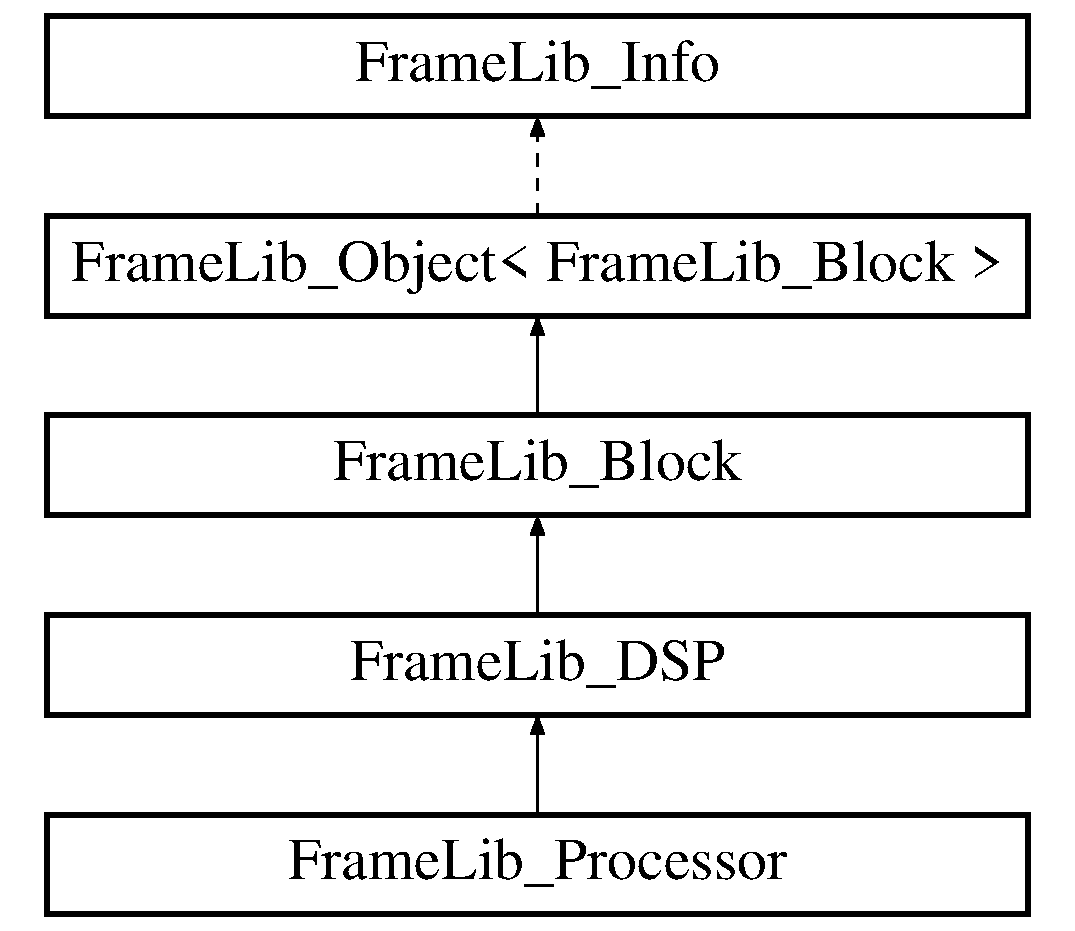
\includegraphics[height=5.000000cm]{class_frame_lib___processor}
\end{center}
\end{figure}
\subsection*{Public Member Functions}
\begin{DoxyCompactItemize}
\item 
\hyperlink{class_frame_lib___processor_aaa48ccb4d8b92b2d51408499e2d52e8c}{Frame\+Lib\+\_\+\+Processor} (\hyperlink{class_frame_lib___context}{Frame\+Lib\+\_\+\+Context} context, \hyperlink{class_frame_lib___parameters_1_1_info}{Frame\+Lib\+\_\+\+Parameters\+::\+Info} $\ast$info, unsigned long n\+Ins=0, unsigned long n\+Outs=0)
\end{DoxyCompactItemize}
\subsection*{Static Public Member Functions}
\begin{DoxyCompactItemize}
\item 
static \hyperlink{_frame_lib___types_8h_a842c5e2e69277690b064bf363c017980}{Object\+Type} \hyperlink{class_frame_lib___processor_a9cf7b310f4d1ca8843b201d692fcf544}{get\+Type} ()
\item 
static bool \hyperlink{class_frame_lib___processor_a77869c3007f363ce914d9e0073953660}{handles\+Audio} ()
\end{DoxyCompactItemize}
\subsection*{Protected Member Functions}
\begin{DoxyCompactItemize}
\item 
virtual \hyperlink{struct_frame_lib___d_s_p_1_1_scheduler_info}{Scheduler\+Info} \hyperlink{class_frame_lib___processor_a2487e6433f6a5e79014664a0500ccc24}{schedule} (bool new\+Frame, bool no\+Advance)
\item 
void \hyperlink{class_frame_lib___processor_a84035040e5e1cff07e16502ee290881e}{set\+IO} (unsigned long n\+Ins, unsigned long n\+Outs)
\end{DoxyCompactItemize}
\subsection*{Additional Inherited Members}


\subsection{Constructor \& Destructor Documentation}
\mbox{\Hypertarget{class_frame_lib___processor_aaa48ccb4d8b92b2d51408499e2d52e8c}\label{class_frame_lib___processor_aaa48ccb4d8b92b2d51408499e2d52e8c}} 
\index{Frame\+Lib\+\_\+\+Processor@{Frame\+Lib\+\_\+\+Processor}!Frame\+Lib\+\_\+\+Processor@{Frame\+Lib\+\_\+\+Processor}}
\index{Frame\+Lib\+\_\+\+Processor@{Frame\+Lib\+\_\+\+Processor}!Frame\+Lib\+\_\+\+Processor@{Frame\+Lib\+\_\+\+Processor}}
\subsubsection{\texorpdfstring{Frame\+Lib\+\_\+\+Processor()}{FrameLib\_Processor()}}
{\footnotesize\ttfamily Frame\+Lib\+\_\+\+Processor\+::\+Frame\+Lib\+\_\+\+Processor (\begin{DoxyParamCaption}\item[{\hyperlink{class_frame_lib___context}{Frame\+Lib\+\_\+\+Context}}]{context,  }\item[{\hyperlink{class_frame_lib___parameters_1_1_info}{Frame\+Lib\+\_\+\+Parameters\+::\+Info} $\ast$}]{info,  }\item[{unsigned long}]{n\+Ins = {\ttfamily 0},  }\item[{unsigned long}]{n\+Outs = {\ttfamily 0} }\end{DoxyParamCaption})\hspace{0.3cm}{\ttfamily [inline]}}



\subsection{Member Function Documentation}
\mbox{\Hypertarget{class_frame_lib___processor_a9cf7b310f4d1ca8843b201d692fcf544}\label{class_frame_lib___processor_a9cf7b310f4d1ca8843b201d692fcf544}} 
\index{Frame\+Lib\+\_\+\+Processor@{Frame\+Lib\+\_\+\+Processor}!get\+Type@{get\+Type}}
\index{get\+Type@{get\+Type}!Frame\+Lib\+\_\+\+Processor@{Frame\+Lib\+\_\+\+Processor}}
\subsubsection{\texorpdfstring{get\+Type()}{getType()}}
{\footnotesize\ttfamily static \hyperlink{_frame_lib___types_8h_a842c5e2e69277690b064bf363c017980}{Object\+Type} Frame\+Lib\+\_\+\+Processor\+::get\+Type (\begin{DoxyParamCaption}{ }\end{DoxyParamCaption})\hspace{0.3cm}{\ttfamily [inline]}, {\ttfamily [static]}}

\mbox{\Hypertarget{class_frame_lib___processor_a77869c3007f363ce914d9e0073953660}\label{class_frame_lib___processor_a77869c3007f363ce914d9e0073953660}} 
\index{Frame\+Lib\+\_\+\+Processor@{Frame\+Lib\+\_\+\+Processor}!handles\+Audio@{handles\+Audio}}
\index{handles\+Audio@{handles\+Audio}!Frame\+Lib\+\_\+\+Processor@{Frame\+Lib\+\_\+\+Processor}}
\subsubsection{\texorpdfstring{handles\+Audio()}{handlesAudio()}}
{\footnotesize\ttfamily static bool Frame\+Lib\+\_\+\+Processor\+::handles\+Audio (\begin{DoxyParamCaption}{ }\end{DoxyParamCaption})\hspace{0.3cm}{\ttfamily [inline]}, {\ttfamily [static]}}

\mbox{\Hypertarget{class_frame_lib___processor_a2487e6433f6a5e79014664a0500ccc24}\label{class_frame_lib___processor_a2487e6433f6a5e79014664a0500ccc24}} 
\index{Frame\+Lib\+\_\+\+Processor@{Frame\+Lib\+\_\+\+Processor}!schedule@{schedule}}
\index{schedule@{schedule}!Frame\+Lib\+\_\+\+Processor@{Frame\+Lib\+\_\+\+Processor}}
\subsubsection{\texorpdfstring{schedule()}{schedule()}}
{\footnotesize\ttfamily virtual \hyperlink{struct_frame_lib___d_s_p_1_1_scheduler_info}{Scheduler\+Info} Frame\+Lib\+\_\+\+Processor\+::schedule (\begin{DoxyParamCaption}\item[{bool}]{new\+Frame,  }\item[{bool}]{no\+Advance }\end{DoxyParamCaption})\hspace{0.3cm}{\ttfamily [inline]}, {\ttfamily [protected]}, {\ttfamily [virtual]}}



Implements \hyperlink{class_frame_lib___d_s_p}{Frame\+Lib\+\_\+\+D\+SP}.

\mbox{\Hypertarget{class_frame_lib___processor_a84035040e5e1cff07e16502ee290881e}\label{class_frame_lib___processor_a84035040e5e1cff07e16502ee290881e}} 
\index{Frame\+Lib\+\_\+\+Processor@{Frame\+Lib\+\_\+\+Processor}!set\+IO@{set\+IO}}
\index{set\+IO@{set\+IO}!Frame\+Lib\+\_\+\+Processor@{Frame\+Lib\+\_\+\+Processor}}
\subsubsection{\texorpdfstring{set\+I\+O()}{setIO()}}
{\footnotesize\ttfamily void Frame\+Lib\+\_\+\+Processor\+::set\+IO (\begin{DoxyParamCaption}\item[{unsigned long}]{n\+Ins,  }\item[{unsigned long}]{n\+Outs }\end{DoxyParamCaption})\hspace{0.3cm}{\ttfamily [inline]}, {\ttfamily [protected]}}



The documentation for this class was generated from the following file\+:\begin{DoxyCompactItemize}
\item 
Frame\+Lib\+\_\+\+Framework/\hyperlink{_frame_lib___d_s_p_8h}{Frame\+Lib\+\_\+\+D\+S\+P.\+h}\end{DoxyCompactItemize}

\hypertarget{class_frame_lib___queueable}{}\section{Frame\+Lib\+\_\+\+Queueable$<$ T $>$ Class Template Reference}
\label{class_frame_lib___queueable}\index{Frame\+Lib\+\_\+\+Queueable$<$ T $>$@{Frame\+Lib\+\_\+\+Queueable$<$ T $>$}}


a template class for items that can be placed on a queue  




{\ttfamily \#include $<$Frame\+Lib\+\_\+\+Object.\+h$>$}

Inheritance diagram for Frame\+Lib\+\_\+\+Queueable$<$ T $>$\+:\begin{figure}[H]
\begin{center}
\leavevmode
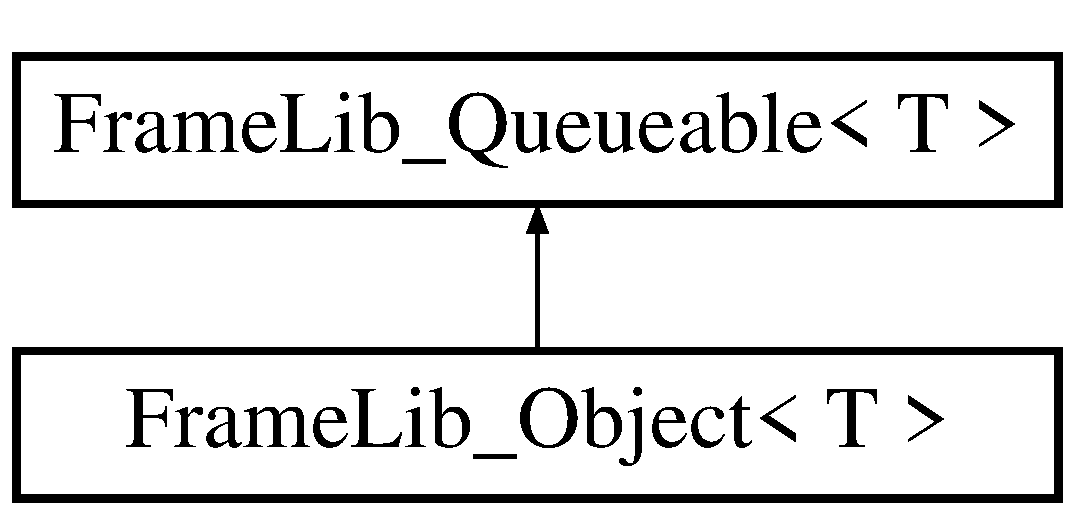
\includegraphics[height=2.000000cm]{class_frame_lib___queueable}
\end{center}
\end{figure}
\subsection*{Classes}
\begin{DoxyCompactItemize}
\item 
class \hyperlink{class_frame_lib___queueable_1_1_queue}{Queue}
\begin{DoxyCompactList}\small\item\em a single-\/threaded queue for non-\/recursive queuing of items for processing \end{DoxyCompactList}\end{DoxyCompactItemize}
\subsection*{Public Member Functions}
\begin{DoxyCompactItemize}
\item 
\hyperlink{class_frame_lib___queueable_ae851e341082e42b5d9f35fce31f51870}{Frame\+Lib\+\_\+\+Queueable} ()
\end{DoxyCompactItemize}


\subsection{Detailed Description}
\subsubsection*{template$<$class T$>$\newline
class Frame\+Lib\+\_\+\+Queueable$<$ T $>$}

a template class for items that can be placed on a queue 

\subsection{Constructor \& Destructor Documentation}
\mbox{\Hypertarget{class_frame_lib___queueable_ae851e341082e42b5d9f35fce31f51870}\label{class_frame_lib___queueable_ae851e341082e42b5d9f35fce31f51870}} 
\index{Frame\+Lib\+\_\+\+Queueable@{Frame\+Lib\+\_\+\+Queueable}!Frame\+Lib\+\_\+\+Queueable@{Frame\+Lib\+\_\+\+Queueable}}
\index{Frame\+Lib\+\_\+\+Queueable@{Frame\+Lib\+\_\+\+Queueable}!Frame\+Lib\+\_\+\+Queueable@{Frame\+Lib\+\_\+\+Queueable}}
\subsubsection{\texorpdfstring{Frame\+Lib\+\_\+\+Queueable()}{FrameLib\_Queueable()}}
{\footnotesize\ttfamily template$<$class T$>$ \\
\hyperlink{class_frame_lib___queueable}{Frame\+Lib\+\_\+\+Queueable}$<$ T $>$\+::\hyperlink{class_frame_lib___queueable}{Frame\+Lib\+\_\+\+Queueable} (\begin{DoxyParamCaption}{ }\end{DoxyParamCaption})\hspace{0.3cm}{\ttfamily [inline]}}



The documentation for this class was generated from the following file\+:\begin{DoxyCompactItemize}
\item 
/\+Users/alexharker/\+Documents/\+Max Externals/\+Frame\+Lib/\+Frame\+Lib\+\_\+\+Framework/\hyperlink{_frame_lib___object_8h}{Frame\+Lib\+\_\+\+Object.\+h}\end{DoxyCompactItemize}

\hypertarget{class_frame_lib___scheduler}{}\section{Frame\+Lib\+\_\+\+Scheduler Class Reference}
\label{class_frame_lib___scheduler}\index{Frame\+Lib\+\_\+\+Scheduler@{Frame\+Lib\+\_\+\+Scheduler}}


{\ttfamily \#include $<$Frame\+Lib\+\_\+\+D\+S\+P.\+h$>$}

Inheritance diagram for Frame\+Lib\+\_\+\+Scheduler\+:\begin{figure}[H]
\begin{center}
\leavevmode
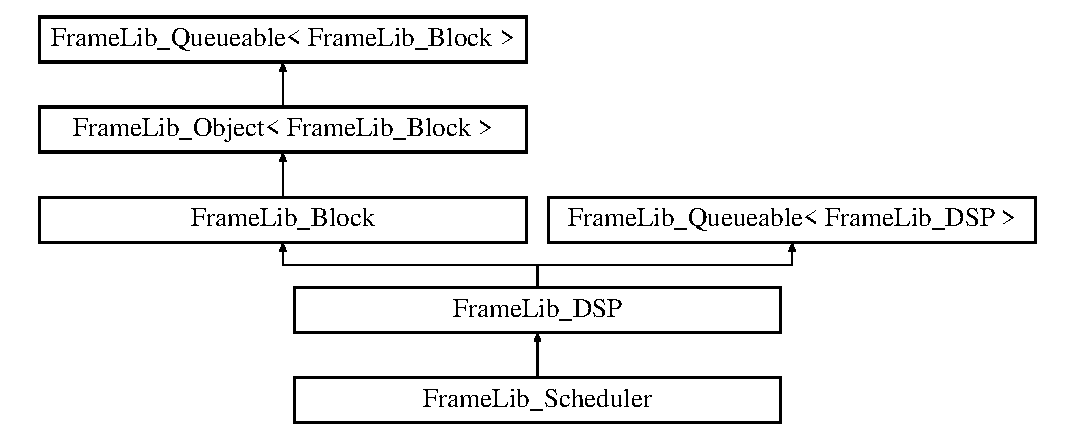
\includegraphics[height=5.000000cm]{class_frame_lib___scheduler}
\end{center}
\end{figure}
\subsection*{Public Member Functions}
\begin{DoxyCompactItemize}
\item 
\hyperlink{class_frame_lib___scheduler_adf967edcf371c60833c9c4dfb0daff1a}{Frame\+Lib\+\_\+\+Scheduler} (\hyperlink{class_frame_lib___context}{Frame\+Lib\+\_\+\+Context} context, void $\ast$owner, \hyperlink{class_frame_lib___parameters_1_1_info}{Frame\+Lib\+\_\+\+Parameters\+::\+Info} $\ast$info, unsigned long n\+Ins=0, unsigned long n\+Outs=0, unsigned long n\+Audio\+Ins=0)
\end{DoxyCompactItemize}
\subsection*{Static Public Member Functions}
\begin{DoxyCompactItemize}
\item 
static \hyperlink{_frame_lib___types_8h_a842c5e2e69277690b064bf363c017980}{Object\+Type} \hyperlink{class_frame_lib___scheduler_a7d93c185e4d7b2d13852dad251dc769b}{get\+Type} ()
\item 
static bool \hyperlink{class_frame_lib___scheduler_a6ab661f5a92b9cc0096af2cde6c6f513}{handles\+Audio} ()
\end{DoxyCompactItemize}
\subsection*{Protected Member Functions}
\begin{DoxyCompactItemize}
\item 
virtual void \hyperlink{class_frame_lib___scheduler_aa5c10907d7d11e1beef86d19b8e93601}{process} ()
\end{DoxyCompactItemize}
\subsection*{Additional Inherited Members}


\subsection{Constructor \& Destructor Documentation}
\mbox{\Hypertarget{class_frame_lib___scheduler_adf967edcf371c60833c9c4dfb0daff1a}\label{class_frame_lib___scheduler_adf967edcf371c60833c9c4dfb0daff1a}} 
\index{Frame\+Lib\+\_\+\+Scheduler@{Frame\+Lib\+\_\+\+Scheduler}!Frame\+Lib\+\_\+\+Scheduler@{Frame\+Lib\+\_\+\+Scheduler}}
\index{Frame\+Lib\+\_\+\+Scheduler@{Frame\+Lib\+\_\+\+Scheduler}!Frame\+Lib\+\_\+\+Scheduler@{Frame\+Lib\+\_\+\+Scheduler}}
\subsubsection{\texorpdfstring{Frame\+Lib\+\_\+\+Scheduler()}{FrameLib\_Scheduler()}}
{\footnotesize\ttfamily Frame\+Lib\+\_\+\+Scheduler\+::\+Frame\+Lib\+\_\+\+Scheduler (\begin{DoxyParamCaption}\item[{\hyperlink{class_frame_lib___context}{Frame\+Lib\+\_\+\+Context}}]{context,  }\item[{void $\ast$}]{owner,  }\item[{\hyperlink{class_frame_lib___parameters_1_1_info}{Frame\+Lib\+\_\+\+Parameters\+::\+Info} $\ast$}]{info,  }\item[{unsigned long}]{n\+Ins = {\ttfamily 0},  }\item[{unsigned long}]{n\+Outs = {\ttfamily 0},  }\item[{unsigned long}]{n\+Audio\+Ins = {\ttfamily 0} }\end{DoxyParamCaption})\hspace{0.3cm}{\ttfamily [inline]}}



\subsection{Member Function Documentation}
\mbox{\Hypertarget{class_frame_lib___scheduler_a7d93c185e4d7b2d13852dad251dc769b}\label{class_frame_lib___scheduler_a7d93c185e4d7b2d13852dad251dc769b}} 
\index{Frame\+Lib\+\_\+\+Scheduler@{Frame\+Lib\+\_\+\+Scheduler}!get\+Type@{get\+Type}}
\index{get\+Type@{get\+Type}!Frame\+Lib\+\_\+\+Scheduler@{Frame\+Lib\+\_\+\+Scheduler}}
\subsubsection{\texorpdfstring{get\+Type()}{getType()}}
{\footnotesize\ttfamily static \hyperlink{_frame_lib___types_8h_a842c5e2e69277690b064bf363c017980}{Object\+Type} Frame\+Lib\+\_\+\+Scheduler\+::get\+Type (\begin{DoxyParamCaption}{ }\end{DoxyParamCaption})\hspace{0.3cm}{\ttfamily [inline]}, {\ttfamily [static]}}

\mbox{\Hypertarget{class_frame_lib___scheduler_a6ab661f5a92b9cc0096af2cde6c6f513}\label{class_frame_lib___scheduler_a6ab661f5a92b9cc0096af2cde6c6f513}} 
\index{Frame\+Lib\+\_\+\+Scheduler@{Frame\+Lib\+\_\+\+Scheduler}!handles\+Audio@{handles\+Audio}}
\index{handles\+Audio@{handles\+Audio}!Frame\+Lib\+\_\+\+Scheduler@{Frame\+Lib\+\_\+\+Scheduler}}
\subsubsection{\texorpdfstring{handles\+Audio()}{handlesAudio()}}
{\footnotesize\ttfamily static bool Frame\+Lib\+\_\+\+Scheduler\+::handles\+Audio (\begin{DoxyParamCaption}{ }\end{DoxyParamCaption})\hspace{0.3cm}{\ttfamily [inline]}, {\ttfamily [static]}}

\mbox{\Hypertarget{class_frame_lib___scheduler_aa5c10907d7d11e1beef86d19b8e93601}\label{class_frame_lib___scheduler_aa5c10907d7d11e1beef86d19b8e93601}} 
\index{Frame\+Lib\+\_\+\+Scheduler@{Frame\+Lib\+\_\+\+Scheduler}!process@{process}}
\index{process@{process}!Frame\+Lib\+\_\+\+Scheduler@{Frame\+Lib\+\_\+\+Scheduler}}
\subsubsection{\texorpdfstring{process()}{process()}}
{\footnotesize\ttfamily virtual void Frame\+Lib\+\_\+\+Scheduler\+::process (\begin{DoxyParamCaption}{ }\end{DoxyParamCaption})\hspace{0.3cm}{\ttfamily [inline]}, {\ttfamily [protected]}, {\ttfamily [virtual]}}



Implements \hyperlink{class_frame_lib___d_s_p}{Frame\+Lib\+\_\+\+D\+SP}.



The documentation for this class was generated from the following file\+:\begin{DoxyCompactItemize}
\item 
/\+Users/alexharker/\+Documents/\+Max Externals/\+Frame\+Lib/\+Frame\+Lib\+\_\+\+Framework/\hyperlink{_frame_lib___d_s_p_8h}{Frame\+Lib\+\_\+\+D\+S\+P.\+h}\end{DoxyCompactItemize}

\hypertarget{class_frame_lib___unpack}{}\section{Frame\+Lib\+\_\+\+Unpack Class Reference}
\label{class_frame_lib___unpack}\index{Frame\+Lib\+\_\+\+Unpack@{Frame\+Lib\+\_\+\+Unpack}}


{\ttfamily \#include $<$Frame\+Lib\+\_\+\+Multichannel.\+h$>$}

Inheritance diagram for Frame\+Lib\+\_\+\+Unpack\+:\begin{figure}[H]
\begin{center}
\leavevmode
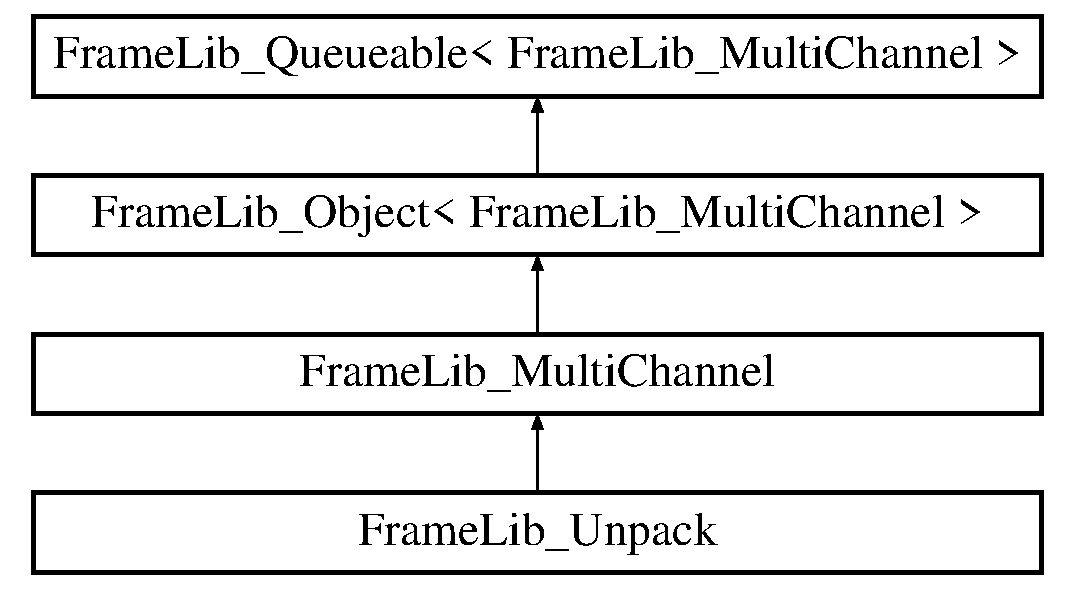
\includegraphics[height=4.000000cm]{class_frame_lib___unpack}
\end{center}
\end{figure}
\subsection*{Public Member Functions}
\begin{DoxyCompactItemize}
\item 
\hyperlink{class_frame_lib___unpack_a987b9186fb9ec69664610f3893063dcc}{Frame\+Lib\+\_\+\+Unpack} (\hyperlink{class_frame_lib___context}{Frame\+Lib\+\_\+\+Context} context, \hyperlink{class_frame_lib___parameters_1_1_serial}{Frame\+Lib\+\_\+\+Parameters\+::\+Serial} $\ast$serialised\+Parameters, void $\ast$owner)
\item 
virtual std\+::string \hyperlink{class_frame_lib___unpack_ab298a6feb7c051f3563a01caacd99c02}{object\+Info} (bool verbose)
\item 
virtual std\+::string \hyperlink{class_frame_lib___unpack_a1ee09b9d9ab16f598f3462d9b29533be}{input\+Info} (unsigned long idx, bool verbose)
\item 
virtual std\+::string \hyperlink{class_frame_lib___unpack_a7e9a710850c3d94d73d00ea27a90d494}{output\+Info} (unsigned long idx, bool verbose)
\item 
virtual const \hyperlink{class_frame_lib___parameters}{Frame\+Lib\+\_\+\+Parameters} $\ast$ \hyperlink{class_frame_lib___unpack_aa9da91c13a8e4d648bdef0037973dc56}{get\+Parameters} ()
\item 
virtual \hyperlink{_frame_lib___types_8h_ad495a9f61af7fff07d7e97979d1ab854}{Frame\+Type} \hyperlink{class_frame_lib___unpack_a003ea8257f11fe375cc9bf2e6b5a8db1}{input\+Type} (unsigned long idx)
\item 
virtual \hyperlink{_frame_lib___types_8h_ad495a9f61af7fff07d7e97979d1ab854}{Frame\+Type} \hyperlink{class_frame_lib___unpack_a7a88aeaeeaa657858c014a685ef901e7}{output\+Type} (unsigned long idx)
\end{DoxyCompactItemize}
\subsection*{Additional Inherited Members}


\subsection{Constructor \& Destructor Documentation}
\mbox{\Hypertarget{class_frame_lib___unpack_a987b9186fb9ec69664610f3893063dcc}\label{class_frame_lib___unpack_a987b9186fb9ec69664610f3893063dcc}} 
\index{Frame\+Lib\+\_\+\+Unpack@{Frame\+Lib\+\_\+\+Unpack}!Frame\+Lib\+\_\+\+Unpack@{Frame\+Lib\+\_\+\+Unpack}}
\index{Frame\+Lib\+\_\+\+Unpack@{Frame\+Lib\+\_\+\+Unpack}!Frame\+Lib\+\_\+\+Unpack@{Frame\+Lib\+\_\+\+Unpack}}
\subsubsection{\texorpdfstring{Frame\+Lib\+\_\+\+Unpack()}{FrameLib\_Unpack()}}
{\footnotesize\ttfamily Frame\+Lib\+\_\+\+Unpack\+::\+Frame\+Lib\+\_\+\+Unpack (\begin{DoxyParamCaption}\item[{\hyperlink{class_frame_lib___context}{Frame\+Lib\+\_\+\+Context}}]{context,  }\item[{\hyperlink{class_frame_lib___parameters_1_1_serial}{Frame\+Lib\+\_\+\+Parameters\+::\+Serial} $\ast$}]{serialised\+Parameters,  }\item[{void $\ast$}]{owner }\end{DoxyParamCaption})}



\subsection{Member Function Documentation}
\mbox{\Hypertarget{class_frame_lib___unpack_aa9da91c13a8e4d648bdef0037973dc56}\label{class_frame_lib___unpack_aa9da91c13a8e4d648bdef0037973dc56}} 
\index{Frame\+Lib\+\_\+\+Unpack@{Frame\+Lib\+\_\+\+Unpack}!get\+Parameters@{get\+Parameters}}
\index{get\+Parameters@{get\+Parameters}!Frame\+Lib\+\_\+\+Unpack@{Frame\+Lib\+\_\+\+Unpack}}
\subsubsection{\texorpdfstring{get\+Parameters()}{getParameters()}}
{\footnotesize\ttfamily virtual const \hyperlink{class_frame_lib___parameters}{Frame\+Lib\+\_\+\+Parameters}$\ast$ Frame\+Lib\+\_\+\+Unpack\+::get\+Parameters (\begin{DoxyParamCaption}{ }\end{DoxyParamCaption})\hspace{0.3cm}{\ttfamily [inline]}, {\ttfamily [virtual]}}



Reimplemented from \hyperlink{class_frame_lib___object_aaebb53211e0617e9203d1088c2fcb9c2}{Frame\+Lib\+\_\+\+Object$<$ Frame\+Lib\+\_\+\+Multi\+Channel $>$}.

\mbox{\Hypertarget{class_frame_lib___unpack_a1ee09b9d9ab16f598f3462d9b29533be}\label{class_frame_lib___unpack_a1ee09b9d9ab16f598f3462d9b29533be}} 
\index{Frame\+Lib\+\_\+\+Unpack@{Frame\+Lib\+\_\+\+Unpack}!input\+Info@{input\+Info}}
\index{input\+Info@{input\+Info}!Frame\+Lib\+\_\+\+Unpack@{Frame\+Lib\+\_\+\+Unpack}}
\subsubsection{\texorpdfstring{input\+Info()}{inputInfo()}}
{\footnotesize\ttfamily std\+::string Frame\+Lib\+\_\+\+Unpack\+::input\+Info (\begin{DoxyParamCaption}\item[{unsigned long}]{idx,  }\item[{bool}]{verbose }\end{DoxyParamCaption})\hspace{0.3cm}{\ttfamily [virtual]}}



Reimplemented from \hyperlink{class_frame_lib___object_a49abea5f18125c425b1eae8710735891}{Frame\+Lib\+\_\+\+Object$<$ Frame\+Lib\+\_\+\+Multi\+Channel $>$}.

\mbox{\Hypertarget{class_frame_lib___unpack_a003ea8257f11fe375cc9bf2e6b5a8db1}\label{class_frame_lib___unpack_a003ea8257f11fe375cc9bf2e6b5a8db1}} 
\index{Frame\+Lib\+\_\+\+Unpack@{Frame\+Lib\+\_\+\+Unpack}!input\+Type@{input\+Type}}
\index{input\+Type@{input\+Type}!Frame\+Lib\+\_\+\+Unpack@{Frame\+Lib\+\_\+\+Unpack}}
\subsubsection{\texorpdfstring{input\+Type()}{inputType()}}
{\footnotesize\ttfamily virtual \hyperlink{_frame_lib___types_8h_ad495a9f61af7fff07d7e97979d1ab854}{Frame\+Type} Frame\+Lib\+\_\+\+Unpack\+::input\+Type (\begin{DoxyParamCaption}\item[{unsigned long}]{idx }\end{DoxyParamCaption})\hspace{0.3cm}{\ttfamily [inline]}, {\ttfamily [virtual]}}



Implements \hyperlink{class_frame_lib___object_a6c5d94f1577471d33204078e86f51ff3}{Frame\+Lib\+\_\+\+Object$<$ Frame\+Lib\+\_\+\+Multi\+Channel $>$}.

\mbox{\Hypertarget{class_frame_lib___unpack_ab298a6feb7c051f3563a01caacd99c02}\label{class_frame_lib___unpack_ab298a6feb7c051f3563a01caacd99c02}} 
\index{Frame\+Lib\+\_\+\+Unpack@{Frame\+Lib\+\_\+\+Unpack}!object\+Info@{object\+Info}}
\index{object\+Info@{object\+Info}!Frame\+Lib\+\_\+\+Unpack@{Frame\+Lib\+\_\+\+Unpack}}
\subsubsection{\texorpdfstring{object\+Info()}{objectInfo()}}
{\footnotesize\ttfamily std\+::string Frame\+Lib\+\_\+\+Unpack\+::object\+Info (\begin{DoxyParamCaption}\item[{bool}]{verbose }\end{DoxyParamCaption})\hspace{0.3cm}{\ttfamily [virtual]}}



Reimplemented from \hyperlink{class_frame_lib___object_a10d673de9a3c59ace6a22ba1cff313c8}{Frame\+Lib\+\_\+\+Object$<$ Frame\+Lib\+\_\+\+Multi\+Channel $>$}.

\mbox{\Hypertarget{class_frame_lib___unpack_a7e9a710850c3d94d73d00ea27a90d494}\label{class_frame_lib___unpack_a7e9a710850c3d94d73d00ea27a90d494}} 
\index{Frame\+Lib\+\_\+\+Unpack@{Frame\+Lib\+\_\+\+Unpack}!output\+Info@{output\+Info}}
\index{output\+Info@{output\+Info}!Frame\+Lib\+\_\+\+Unpack@{Frame\+Lib\+\_\+\+Unpack}}
\subsubsection{\texorpdfstring{output\+Info()}{outputInfo()}}
{\footnotesize\ttfamily std\+::string Frame\+Lib\+\_\+\+Unpack\+::output\+Info (\begin{DoxyParamCaption}\item[{unsigned long}]{idx,  }\item[{bool}]{verbose }\end{DoxyParamCaption})\hspace{0.3cm}{\ttfamily [virtual]}}



Reimplemented from \hyperlink{class_frame_lib___object_a6e6d79e8d620eedbaa50abf324cdedf5}{Frame\+Lib\+\_\+\+Object$<$ Frame\+Lib\+\_\+\+Multi\+Channel $>$}.

\mbox{\Hypertarget{class_frame_lib___unpack_a7a88aeaeeaa657858c014a685ef901e7}\label{class_frame_lib___unpack_a7a88aeaeeaa657858c014a685ef901e7}} 
\index{Frame\+Lib\+\_\+\+Unpack@{Frame\+Lib\+\_\+\+Unpack}!output\+Type@{output\+Type}}
\index{output\+Type@{output\+Type}!Frame\+Lib\+\_\+\+Unpack@{Frame\+Lib\+\_\+\+Unpack}}
\subsubsection{\texorpdfstring{output\+Type()}{outputType()}}
{\footnotesize\ttfamily virtual \hyperlink{_frame_lib___types_8h_ad495a9f61af7fff07d7e97979d1ab854}{Frame\+Type} Frame\+Lib\+\_\+\+Unpack\+::output\+Type (\begin{DoxyParamCaption}\item[{unsigned long}]{idx }\end{DoxyParamCaption})\hspace{0.3cm}{\ttfamily [inline]}, {\ttfamily [virtual]}}



Implements \hyperlink{class_frame_lib___object_abdfca6b259f5fc7f97f4f2e016c1d80f}{Frame\+Lib\+\_\+\+Object$<$ Frame\+Lib\+\_\+\+Multi\+Channel $>$}.



The documentation for this class was generated from the following files\+:\begin{DoxyCompactItemize}
\item 
Frame\+Lib\+\_\+\+Framework/\hyperlink{_frame_lib___multichannel_8h}{Frame\+Lib\+\_\+\+Multichannel.\+h}\item 
Frame\+Lib\+\_\+\+Framework/\hyperlink{_frame_lib___multichannel_8cpp}{Frame\+Lib\+\_\+\+Multichannel.\+cpp}\end{DoxyCompactItemize}

\hypertarget{class_frame_lib___parameters_1_1_info}{}\section{Frame\+Lib\+\_\+\+Parameters\+:\+:Info Class Reference}
\label{class_frame_lib___parameters_1_1_info}\index{Frame\+Lib\+\_\+\+Parameters\+::\+Info@{Frame\+Lib\+\_\+\+Parameters\+::\+Info}}


a class for passing info strings to \hyperlink{class_frame_lib___parameters}{Frame\+Lib\+\_\+\+Parameters}.  




{\ttfamily \#include $<$Frame\+Lib\+\_\+\+Parameters.\+h$>$}

\subsection*{Public Member Functions}
\begin{DoxyCompactItemize}
\item 
void \hyperlink{class_frame_lib___parameters_1_1_info_a7d2360d181ac4e0d8e49af6b5777b38b}{add} (const char $\ast$str)
\item 
void \hyperlink{class_frame_lib___parameters_1_1_info_ae5b7b0ee9401ba93b5a15cc25f0f7863}{add} (const std\+::string \&str)
\item 
const char $\ast$ \hyperlink{class_frame_lib___parameters_1_1_info_a1f1518215e8de95d2e587de919ff47f0}{get} (unsigned long idx)
\end{DoxyCompactItemize}


\subsection{Detailed Description}
a class for passing info strings to \hyperlink{class_frame_lib___parameters}{Frame\+Lib\+\_\+\+Parameters}. 

\subsection{Member Function Documentation}
\mbox{\Hypertarget{class_frame_lib___parameters_1_1_info_a7d2360d181ac4e0d8e49af6b5777b38b}\label{class_frame_lib___parameters_1_1_info_a7d2360d181ac4e0d8e49af6b5777b38b}} 
\index{Frame\+Lib\+\_\+\+Parameters\+::\+Info@{Frame\+Lib\+\_\+\+Parameters\+::\+Info}!add@{add}}
\index{add@{add}!Frame\+Lib\+\_\+\+Parameters\+::\+Info@{Frame\+Lib\+\_\+\+Parameters\+::\+Info}}
\subsubsection{\texorpdfstring{add()}{add()}\hspace{0.1cm}{\footnotesize\ttfamily [1/2]}}
{\footnotesize\ttfamily void Frame\+Lib\+\_\+\+Parameters\+::\+Info\+::add (\begin{DoxyParamCaption}\item[{const char $\ast$}]{str }\end{DoxyParamCaption})\hspace{0.3cm}{\ttfamily [inline]}}

\mbox{\Hypertarget{class_frame_lib___parameters_1_1_info_ae5b7b0ee9401ba93b5a15cc25f0f7863}\label{class_frame_lib___parameters_1_1_info_ae5b7b0ee9401ba93b5a15cc25f0f7863}} 
\index{Frame\+Lib\+\_\+\+Parameters\+::\+Info@{Frame\+Lib\+\_\+\+Parameters\+::\+Info}!add@{add}}
\index{add@{add}!Frame\+Lib\+\_\+\+Parameters\+::\+Info@{Frame\+Lib\+\_\+\+Parameters\+::\+Info}}
\subsubsection{\texorpdfstring{add()}{add()}\hspace{0.1cm}{\footnotesize\ttfamily [2/2]}}
{\footnotesize\ttfamily void Frame\+Lib\+\_\+\+Parameters\+::\+Info\+::add (\begin{DoxyParamCaption}\item[{const std\+::string \&}]{str }\end{DoxyParamCaption})\hspace{0.3cm}{\ttfamily [inline]}}

\mbox{\Hypertarget{class_frame_lib___parameters_1_1_info_a1f1518215e8de95d2e587de919ff47f0}\label{class_frame_lib___parameters_1_1_info_a1f1518215e8de95d2e587de919ff47f0}} 
\index{Frame\+Lib\+\_\+\+Parameters\+::\+Info@{Frame\+Lib\+\_\+\+Parameters\+::\+Info}!get@{get}}
\index{get@{get}!Frame\+Lib\+\_\+\+Parameters\+::\+Info@{Frame\+Lib\+\_\+\+Parameters\+::\+Info}}
\subsubsection{\texorpdfstring{get()}{get()}}
{\footnotesize\ttfamily const char$\ast$ Frame\+Lib\+\_\+\+Parameters\+::\+Info\+::get (\begin{DoxyParamCaption}\item[{unsigned long}]{idx }\end{DoxyParamCaption})\hspace{0.3cm}{\ttfamily [inline]}}



The documentation for this class was generated from the following file\+:\begin{DoxyCompactItemize}
\item 
/\+Users/alexharker/\+Documents/\+Max Externals/\+Frame\+Lib/\+Frame\+Lib\+\_\+\+Framework/\hyperlink{_frame_lib___parameters_8h}{Frame\+Lib\+\_\+\+Parameters.\+h}\end{DoxyCompactItemize}

\hypertarget{class_frame_lib___global_allocator_1_1_pruner}{}\section{Frame\+Lib\+\_\+\+Global\+Allocator\+:\+:Pruner Class Reference}
\label{class_frame_lib___global_allocator_1_1_pruner}\index{Frame\+Lib\+\_\+\+Global\+Allocator\+::\+Pruner@{Frame\+Lib\+\_\+\+Global\+Allocator\+::\+Pruner}}


{\ttfamily \#include $<$Frame\+Lib\+\_\+\+Memory.\+h$>$}

\subsection*{Public Member Functions}
\begin{DoxyCompactItemize}
\item 
\hyperlink{class_frame_lib___global_allocator_1_1_pruner_aaeef6460d559456c61e25854f016625c}{Pruner} (\hyperlink{class_frame_lib___global_allocator}{Frame\+Lib\+\_\+\+Global\+Allocator} $\ast$allocator)
\item 
\hyperlink{class_frame_lib___global_allocator_1_1_pruner_af1b947e70e93d005e5a996ea2010e51a}{$\sim$\+Pruner} ()
\item 
void \hyperlink{class_frame_lib___global_allocator_1_1_pruner_ad261c2fb12e19ce40ed3af4c550c479c}{dealloc} (void $\ast$ptr)
\end{DoxyCompactItemize}


\subsection{Constructor \& Destructor Documentation}
\mbox{\Hypertarget{class_frame_lib___global_allocator_1_1_pruner_aaeef6460d559456c61e25854f016625c}\label{class_frame_lib___global_allocator_1_1_pruner_aaeef6460d559456c61e25854f016625c}} 
\index{Frame\+Lib\+\_\+\+Global\+Allocator\+::\+Pruner@{Frame\+Lib\+\_\+\+Global\+Allocator\+::\+Pruner}!Pruner@{Pruner}}
\index{Pruner@{Pruner}!Frame\+Lib\+\_\+\+Global\+Allocator\+::\+Pruner@{Frame\+Lib\+\_\+\+Global\+Allocator\+::\+Pruner}}
\subsubsection{\texorpdfstring{Pruner()}{Pruner()}}
{\footnotesize\ttfamily Frame\+Lib\+\_\+\+Global\+Allocator\+::\+Pruner\+::\+Pruner (\begin{DoxyParamCaption}\item[{\hyperlink{class_frame_lib___global_allocator}{Frame\+Lib\+\_\+\+Global\+Allocator} $\ast$}]{allocator }\end{DoxyParamCaption})\hspace{0.3cm}{\ttfamily [inline]}}

\mbox{\Hypertarget{class_frame_lib___global_allocator_1_1_pruner_af1b947e70e93d005e5a996ea2010e51a}\label{class_frame_lib___global_allocator_1_1_pruner_af1b947e70e93d005e5a996ea2010e51a}} 
\index{Frame\+Lib\+\_\+\+Global\+Allocator\+::\+Pruner@{Frame\+Lib\+\_\+\+Global\+Allocator\+::\+Pruner}!````~Pruner@{$\sim$\+Pruner}}
\index{````~Pruner@{$\sim$\+Pruner}!Frame\+Lib\+\_\+\+Global\+Allocator\+::\+Pruner@{Frame\+Lib\+\_\+\+Global\+Allocator\+::\+Pruner}}
\subsubsection{\texorpdfstring{$\sim$\+Pruner()}{~Pruner()}}
{\footnotesize\ttfamily Frame\+Lib\+\_\+\+Global\+Allocator\+::\+Pruner\+::$\sim$\+Pruner (\begin{DoxyParamCaption}{ }\end{DoxyParamCaption})\hspace{0.3cm}{\ttfamily [inline]}}



\subsection{Member Function Documentation}
\mbox{\Hypertarget{class_frame_lib___global_allocator_1_1_pruner_ad261c2fb12e19ce40ed3af4c550c479c}\label{class_frame_lib___global_allocator_1_1_pruner_ad261c2fb12e19ce40ed3af4c550c479c}} 
\index{Frame\+Lib\+\_\+\+Global\+Allocator\+::\+Pruner@{Frame\+Lib\+\_\+\+Global\+Allocator\+::\+Pruner}!dealloc@{dealloc}}
\index{dealloc@{dealloc}!Frame\+Lib\+\_\+\+Global\+Allocator\+::\+Pruner@{Frame\+Lib\+\_\+\+Global\+Allocator\+::\+Pruner}}
\subsubsection{\texorpdfstring{dealloc()}{dealloc()}}
{\footnotesize\ttfamily void Frame\+Lib\+\_\+\+Global\+Allocator\+::\+Pruner\+::dealloc (\begin{DoxyParamCaption}\item[{void $\ast$}]{ptr }\end{DoxyParamCaption})\hspace{0.3cm}{\ttfamily [inline]}}



The documentation for this class was generated from the following file\+:\begin{DoxyCompactItemize}
\item 
Frame\+Lib\+\_\+\+Framework/\hyperlink{_frame_lib___memory_8h}{Frame\+Lib\+\_\+\+Memory.\+h}\end{DoxyCompactItemize}

\hypertarget{class_frame_lib___queueable_1_1_queue}{}\section{Frame\+Lib\+\_\+\+Queueable$<$ T $>$\+:\+:Queue Class Reference}
\label{class_frame_lib___queueable_1_1_queue}\index{Frame\+Lib\+\_\+\+Queueable$<$ T $>$\+::\+Queue@{Frame\+Lib\+\_\+\+Queueable$<$ T $>$\+::\+Queue}}


{\ttfamily \#include $<$Frame\+Lib\+\_\+\+Object.\+h$>$}

\subsection*{Public Member Functions}
\begin{DoxyCompactItemize}
\item 
\hyperlink{class_frame_lib___queueable_1_1_queue_a5eb25b5751d5cc25331aa5e1b4fcb6ae}{Queue} ()
\item 
\hyperlink{class_frame_lib___queueable_1_1_queue_af701d261343c894ba4cde0aa8dd99bd1}{Queue} (T $\ast$object, Method method)
\item 
void \hyperlink{class_frame_lib___queueable_1_1_queue_abf0d41d8f1e7988e1bde9b8a5f899f30}{add} (T $\ast$object, Method method)
\item 
T $\ast$ \hyperlink{class_frame_lib___queueable_1_1_queue_a57e16be316a37b9b6d0d5cf7267e4d12}{get\+First} () const
\end{DoxyCompactItemize}


\subsection{Constructor \& Destructor Documentation}
\mbox{\Hypertarget{class_frame_lib___queueable_1_1_queue_a5eb25b5751d5cc25331aa5e1b4fcb6ae}\label{class_frame_lib___queueable_1_1_queue_a5eb25b5751d5cc25331aa5e1b4fcb6ae}} 
\index{Frame\+Lib\+\_\+\+Queueable\+::\+Queue@{Frame\+Lib\+\_\+\+Queueable\+::\+Queue}!Queue@{Queue}}
\index{Queue@{Queue}!Frame\+Lib\+\_\+\+Queueable\+::\+Queue@{Frame\+Lib\+\_\+\+Queueable\+::\+Queue}}
\subsubsection{\texorpdfstring{Queue()}{Queue()}\hspace{0.1cm}{\footnotesize\ttfamily [1/2]}}
{\footnotesize\ttfamily template$<$class T$>$ \\
\hyperlink{class_frame_lib___queueable}{Frame\+Lib\+\_\+\+Queueable}$<$ T $>$\+::Queue\+::\+Queue (\begin{DoxyParamCaption}{ }\end{DoxyParamCaption})\hspace{0.3cm}{\ttfamily [inline]}}

\mbox{\Hypertarget{class_frame_lib___queueable_1_1_queue_af701d261343c894ba4cde0aa8dd99bd1}\label{class_frame_lib___queueable_1_1_queue_af701d261343c894ba4cde0aa8dd99bd1}} 
\index{Frame\+Lib\+\_\+\+Queueable\+::\+Queue@{Frame\+Lib\+\_\+\+Queueable\+::\+Queue}!Queue@{Queue}}
\index{Queue@{Queue}!Frame\+Lib\+\_\+\+Queueable\+::\+Queue@{Frame\+Lib\+\_\+\+Queueable\+::\+Queue}}
\subsubsection{\texorpdfstring{Queue()}{Queue()}\hspace{0.1cm}{\footnotesize\ttfamily [2/2]}}
{\footnotesize\ttfamily template$<$class T$>$ \\
\hyperlink{class_frame_lib___queueable}{Frame\+Lib\+\_\+\+Queueable}$<$ T $>$\+::Queue\+::\+Queue (\begin{DoxyParamCaption}\item[{T $\ast$}]{object,  }\item[{Method}]{method }\end{DoxyParamCaption})\hspace{0.3cm}{\ttfamily [inline]}}



\subsection{Member Function Documentation}
\mbox{\Hypertarget{class_frame_lib___queueable_1_1_queue_abf0d41d8f1e7988e1bde9b8a5f899f30}\label{class_frame_lib___queueable_1_1_queue_abf0d41d8f1e7988e1bde9b8a5f899f30}} 
\index{Frame\+Lib\+\_\+\+Queueable\+::\+Queue@{Frame\+Lib\+\_\+\+Queueable\+::\+Queue}!add@{add}}
\index{add@{add}!Frame\+Lib\+\_\+\+Queueable\+::\+Queue@{Frame\+Lib\+\_\+\+Queueable\+::\+Queue}}
\subsubsection{\texorpdfstring{add()}{add()}}
{\footnotesize\ttfamily template$<$class T$>$ \\
void \hyperlink{class_frame_lib___queueable}{Frame\+Lib\+\_\+\+Queueable}$<$ T $>$\+::Queue\+::add (\begin{DoxyParamCaption}\item[{T $\ast$}]{object,  }\item[{Method}]{method }\end{DoxyParamCaption})\hspace{0.3cm}{\ttfamily [inline]}}

\mbox{\Hypertarget{class_frame_lib___queueable_1_1_queue_a57e16be316a37b9b6d0d5cf7267e4d12}\label{class_frame_lib___queueable_1_1_queue_a57e16be316a37b9b6d0d5cf7267e4d12}} 
\index{Frame\+Lib\+\_\+\+Queueable\+::\+Queue@{Frame\+Lib\+\_\+\+Queueable\+::\+Queue}!get\+First@{get\+First}}
\index{get\+First@{get\+First}!Frame\+Lib\+\_\+\+Queueable\+::\+Queue@{Frame\+Lib\+\_\+\+Queueable\+::\+Queue}}
\subsubsection{\texorpdfstring{get\+First()}{getFirst()}}
{\footnotesize\ttfamily template$<$class T$>$ \\
T$\ast$ \hyperlink{class_frame_lib___queueable}{Frame\+Lib\+\_\+\+Queueable}$<$ T $>$\+::Queue\+::get\+First (\begin{DoxyParamCaption}{ }\end{DoxyParamCaption}) const\hspace{0.3cm}{\ttfamily [inline]}}



The documentation for this class was generated from the following file\+:\begin{DoxyCompactItemize}
\item 
/\+Users/alexharker/\+Documents/\+Max Externals/\+Frame\+Lib/\+Frame\+Lib\+\_\+\+Framework/\hyperlink{_frame_lib___object_8h}{Frame\+Lib\+\_\+\+Object.\+h}\end{DoxyCompactItemize}

\hypertarget{struct_frame_lib___d_s_p_1_1_scheduler_info}{}\section{Frame\+Lib\+\_\+\+D\+SP\+:\+:Scheduler\+Info Struct Reference}
\label{struct_frame_lib___d_s_p_1_1_scheduler_info}\index{Frame\+Lib\+\_\+\+D\+S\+P\+::\+Scheduler\+Info@{Frame\+Lib\+\_\+\+D\+S\+P\+::\+Scheduler\+Info}}


{\ttfamily \#include $<$Frame\+Lib\+\_\+\+D\+S\+P.\+h$>$}

\subsection*{Public Member Functions}
\begin{DoxyCompactItemize}
\item 
\hyperlink{struct_frame_lib___d_s_p_1_1_scheduler_info_a5939a752d4ea50eea67c019805254a82}{Scheduler\+Info} ()
\item 
\hyperlink{struct_frame_lib___d_s_p_1_1_scheduler_info_a82a4ba6533c2d663620c4276b7d27dce}{Scheduler\+Info} (\hyperlink{_frame_lib___types_8h_a699a4071a9eaaa283906a5ebd0a79ac0}{Frame\+Lib\+\_\+\+Time\+Format} time\+Advance, bool new\+Frame, bool output\+Done)
\end{DoxyCompactItemize}
\subsection*{Public Attributes}
\begin{DoxyCompactItemize}
\item 
\hyperlink{_frame_lib___types_8h_a699a4071a9eaaa283906a5ebd0a79ac0}{Frame\+Lib\+\_\+\+Time\+Format} \hyperlink{struct_frame_lib___d_s_p_1_1_scheduler_info_ae38d8335efc201f8c2c967ffea7b6076}{m\+Time\+Advance}
\item 
bool \hyperlink{struct_frame_lib___d_s_p_1_1_scheduler_info_a88fa8b1c2060d60f4ae1cf164405c85f}{m\+New\+Frame}
\item 
bool \hyperlink{struct_frame_lib___d_s_p_1_1_scheduler_info_aee41d636cde5b117b4ce8610905d668d}{m\+Output\+Done}
\end{DoxyCompactItemize}


\subsection{Constructor \& Destructor Documentation}
\mbox{\Hypertarget{struct_frame_lib___d_s_p_1_1_scheduler_info_a5939a752d4ea50eea67c019805254a82}\label{struct_frame_lib___d_s_p_1_1_scheduler_info_a5939a752d4ea50eea67c019805254a82}} 
\index{Frame\+Lib\+\_\+\+D\+S\+P\+::\+Scheduler\+Info@{Frame\+Lib\+\_\+\+D\+S\+P\+::\+Scheduler\+Info}!Scheduler\+Info@{Scheduler\+Info}}
\index{Scheduler\+Info@{Scheduler\+Info}!Frame\+Lib\+\_\+\+D\+S\+P\+::\+Scheduler\+Info@{Frame\+Lib\+\_\+\+D\+S\+P\+::\+Scheduler\+Info}}
\subsubsection{\texorpdfstring{Scheduler\+Info()}{SchedulerInfo()}\hspace{0.1cm}{\footnotesize\ttfamily [1/2]}}
{\footnotesize\ttfamily Frame\+Lib\+\_\+\+D\+S\+P\+::\+Scheduler\+Info\+::\+Scheduler\+Info (\begin{DoxyParamCaption}{ }\end{DoxyParamCaption})\hspace{0.3cm}{\ttfamily [inline]}}

\mbox{\Hypertarget{struct_frame_lib___d_s_p_1_1_scheduler_info_a82a4ba6533c2d663620c4276b7d27dce}\label{struct_frame_lib___d_s_p_1_1_scheduler_info_a82a4ba6533c2d663620c4276b7d27dce}} 
\index{Frame\+Lib\+\_\+\+D\+S\+P\+::\+Scheduler\+Info@{Frame\+Lib\+\_\+\+D\+S\+P\+::\+Scheduler\+Info}!Scheduler\+Info@{Scheduler\+Info}}
\index{Scheduler\+Info@{Scheduler\+Info}!Frame\+Lib\+\_\+\+D\+S\+P\+::\+Scheduler\+Info@{Frame\+Lib\+\_\+\+D\+S\+P\+::\+Scheduler\+Info}}
\subsubsection{\texorpdfstring{Scheduler\+Info()}{SchedulerInfo()}\hspace{0.1cm}{\footnotesize\ttfamily [2/2]}}
{\footnotesize\ttfamily Frame\+Lib\+\_\+\+D\+S\+P\+::\+Scheduler\+Info\+::\+Scheduler\+Info (\begin{DoxyParamCaption}\item[{\hyperlink{_frame_lib___types_8h_a699a4071a9eaaa283906a5ebd0a79ac0}{Frame\+Lib\+\_\+\+Time\+Format}}]{time\+Advance,  }\item[{bool}]{new\+Frame,  }\item[{bool}]{output\+Done }\end{DoxyParamCaption})\hspace{0.3cm}{\ttfamily [inline]}}



\subsection{Member Data Documentation}
\mbox{\Hypertarget{struct_frame_lib___d_s_p_1_1_scheduler_info_a88fa8b1c2060d60f4ae1cf164405c85f}\label{struct_frame_lib___d_s_p_1_1_scheduler_info_a88fa8b1c2060d60f4ae1cf164405c85f}} 
\index{Frame\+Lib\+\_\+\+D\+S\+P\+::\+Scheduler\+Info@{Frame\+Lib\+\_\+\+D\+S\+P\+::\+Scheduler\+Info}!m\+New\+Frame@{m\+New\+Frame}}
\index{m\+New\+Frame@{m\+New\+Frame}!Frame\+Lib\+\_\+\+D\+S\+P\+::\+Scheduler\+Info@{Frame\+Lib\+\_\+\+D\+S\+P\+::\+Scheduler\+Info}}
\subsubsection{\texorpdfstring{m\+New\+Frame}{mNewFrame}}
{\footnotesize\ttfamily bool Frame\+Lib\+\_\+\+D\+S\+P\+::\+Scheduler\+Info\+::m\+New\+Frame}

\mbox{\Hypertarget{struct_frame_lib___d_s_p_1_1_scheduler_info_aee41d636cde5b117b4ce8610905d668d}\label{struct_frame_lib___d_s_p_1_1_scheduler_info_aee41d636cde5b117b4ce8610905d668d}} 
\index{Frame\+Lib\+\_\+\+D\+S\+P\+::\+Scheduler\+Info@{Frame\+Lib\+\_\+\+D\+S\+P\+::\+Scheduler\+Info}!m\+Output\+Done@{m\+Output\+Done}}
\index{m\+Output\+Done@{m\+Output\+Done}!Frame\+Lib\+\_\+\+D\+S\+P\+::\+Scheduler\+Info@{Frame\+Lib\+\_\+\+D\+S\+P\+::\+Scheduler\+Info}}
\subsubsection{\texorpdfstring{m\+Output\+Done}{mOutputDone}}
{\footnotesize\ttfamily bool Frame\+Lib\+\_\+\+D\+S\+P\+::\+Scheduler\+Info\+::m\+Output\+Done}

\mbox{\Hypertarget{struct_frame_lib___d_s_p_1_1_scheduler_info_ae38d8335efc201f8c2c967ffea7b6076}\label{struct_frame_lib___d_s_p_1_1_scheduler_info_ae38d8335efc201f8c2c967ffea7b6076}} 
\index{Frame\+Lib\+\_\+\+D\+S\+P\+::\+Scheduler\+Info@{Frame\+Lib\+\_\+\+D\+S\+P\+::\+Scheduler\+Info}!m\+Time\+Advance@{m\+Time\+Advance}}
\index{m\+Time\+Advance@{m\+Time\+Advance}!Frame\+Lib\+\_\+\+D\+S\+P\+::\+Scheduler\+Info@{Frame\+Lib\+\_\+\+D\+S\+P\+::\+Scheduler\+Info}}
\subsubsection{\texorpdfstring{m\+Time\+Advance}{mTimeAdvance}}
{\footnotesize\ttfamily \hyperlink{_frame_lib___types_8h_a699a4071a9eaaa283906a5ebd0a79ac0}{Frame\+Lib\+\_\+\+Time\+Format} Frame\+Lib\+\_\+\+D\+S\+P\+::\+Scheduler\+Info\+::m\+Time\+Advance}



The documentation for this struct was generated from the following file\+:\begin{DoxyCompactItemize}
\item 
/\+Users/alexharker/\+Documents/\+Max Externals/\+Frame\+Lib/\+Frame\+Lib\+\_\+\+Framework/\hyperlink{_frame_lib___d_s_p_8h}{Frame\+Lib\+\_\+\+D\+S\+P.\+h}\end{DoxyCompactItemize}

\hypertarget{class_semaphore}{}\section{Semaphore Class Reference}
\label{class_semaphore}\index{Semaphore@{Semaphore}}


{\ttfamily \#include $<$Frame\+Lib\+\_\+\+Threading.\+h$>$}

\subsection*{Public Member Functions}
\begin{DoxyCompactItemize}
\item 
\hyperlink{class_semaphore_ab1a0d6b277f585116f7f077b15d09fbf}{Semaphore} (long max\+Count)
\item 
\hyperlink{class_semaphore_a633658a6fde276bffc912028725c6ade}{$\sim$\+Semaphore} ()
\item 
void \hyperlink{class_semaphore_ab04c0934fbf281eb49bd332ecd07c856}{close} ()
\item 
void \hyperlink{class_semaphore_adcd7d652d882d0ab4b068070235ef079}{signal} (long n)
\item 
bool \hyperlink{class_semaphore_a496aae0d0eceef9385c9dcae4c3d9b36}{wait} ()
\end{DoxyCompactItemize}


\subsection{Constructor \& Destructor Documentation}
\mbox{\Hypertarget{class_semaphore_ab1a0d6b277f585116f7f077b15d09fbf}\label{class_semaphore_ab1a0d6b277f585116f7f077b15d09fbf}} 
\index{Semaphore@{Semaphore}!Semaphore@{Semaphore}}
\index{Semaphore@{Semaphore}!Semaphore@{Semaphore}}
\subsubsection{\texorpdfstring{Semaphore()}{Semaphore()}}
{\footnotesize\ttfamily Semaphore\+::\+Semaphore (\begin{DoxyParamCaption}\item[{long}]{max\+Count }\end{DoxyParamCaption})}

\mbox{\Hypertarget{class_semaphore_a633658a6fde276bffc912028725c6ade}\label{class_semaphore_a633658a6fde276bffc912028725c6ade}} 
\index{Semaphore@{Semaphore}!````~Semaphore@{$\sim$\+Semaphore}}
\index{````~Semaphore@{$\sim$\+Semaphore}!Semaphore@{Semaphore}}
\subsubsection{\texorpdfstring{$\sim$\+Semaphore()}{~Semaphore()}}
{\footnotesize\ttfamily Semaphore\+::$\sim$\+Semaphore (\begin{DoxyParamCaption}{ }\end{DoxyParamCaption})}



\subsection{Member Function Documentation}
\mbox{\Hypertarget{class_semaphore_ab04c0934fbf281eb49bd332ecd07c856}\label{class_semaphore_ab04c0934fbf281eb49bd332ecd07c856}} 
\index{Semaphore@{Semaphore}!close@{close}}
\index{close@{close}!Semaphore@{Semaphore}}
\subsubsection{\texorpdfstring{close()}{close()}}
{\footnotesize\ttfamily void Semaphore\+::close (\begin{DoxyParamCaption}{ }\end{DoxyParamCaption})}

\mbox{\Hypertarget{class_semaphore_adcd7d652d882d0ab4b068070235ef079}\label{class_semaphore_adcd7d652d882d0ab4b068070235ef079}} 
\index{Semaphore@{Semaphore}!signal@{signal}}
\index{signal@{signal}!Semaphore@{Semaphore}}
\subsubsection{\texorpdfstring{signal()}{signal()}}
{\footnotesize\ttfamily void Semaphore\+::signal (\begin{DoxyParamCaption}\item[{long}]{n }\end{DoxyParamCaption})}

\mbox{\Hypertarget{class_semaphore_a496aae0d0eceef9385c9dcae4c3d9b36}\label{class_semaphore_a496aae0d0eceef9385c9dcae4c3d9b36}} 
\index{Semaphore@{Semaphore}!wait@{wait}}
\index{wait@{wait}!Semaphore@{Semaphore}}
\subsubsection{\texorpdfstring{wait()}{wait()}}
{\footnotesize\ttfamily bool Semaphore\+::wait (\begin{DoxyParamCaption}{ }\end{DoxyParamCaption})}



The documentation for this class was generated from the following files\+:\begin{DoxyCompactItemize}
\item 
/\+Users/alexharker/\+Documents/\+Max Externals/\+Frame\+Lib/\+Frame\+Lib\+\_\+\+Framework/\hyperlink{_frame_lib___threading_8h}{Frame\+Lib\+\_\+\+Threading.\+h}\item 
/\+Users/alexharker/\+Documents/\+Max Externals/\+Frame\+Lib/\+Frame\+Lib\+\_\+\+Framework/\hyperlink{_frame_lib___threading_8cpp}{Frame\+Lib\+\_\+\+Threading.\+cpp}\end{DoxyCompactItemize}

\hypertarget{class_frame_lib___parameters_1_1_serial}{}\section{Frame\+Lib\+\_\+\+Parameters\+:\+:Serial Class Reference}
\label{class_frame_lib___parameters_1_1_serial}\index{Frame\+Lib\+\_\+\+Parameters\+::\+Serial@{Frame\+Lib\+\_\+\+Parameters\+::\+Serial}}


{\ttfamily \#include $<$Frame\+Lib\+\_\+\+Parameters.\+h$>$}

Inheritance diagram for Frame\+Lib\+\_\+\+Parameters\+:\+:Serial\+:\begin{figure}[H]
\begin{center}
\leavevmode
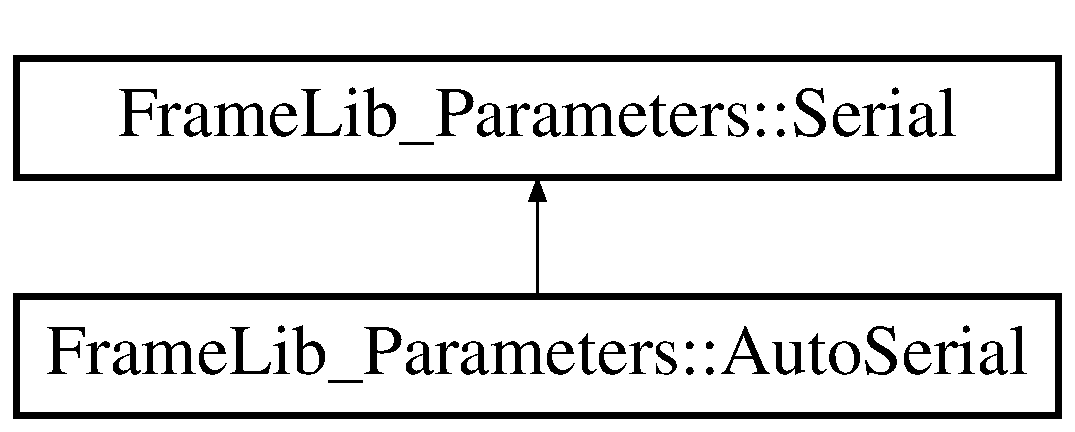
\includegraphics[height=2.000000cm]{class_frame_lib___parameters_1_1_serial}
\end{center}
\end{figure}
\subsection*{Public Member Functions}
\begin{DoxyCompactItemize}
\item 
\hyperlink{class_frame_lib___parameters_1_1_serial_a240eb02a38ab2e545c088f63df9f1851}{Serial} (\hyperlink{_frame_lib___types_8h_a2c5689a997a12479b7d925e565428141}{Byte\+Pointer} ptr, size\+\_\+t \hyperlink{class_frame_lib___parameters_1_1_serial_a04ad46904d9fd8119283eae663901886}{size})
\item 
\hyperlink{class_frame_lib___parameters_1_1_serial_af433868e4f3db5ef6581e3aae7b430a6}{Serial} ()
\item 
void \hyperlink{class_frame_lib___parameters_1_1_serial_ac06dc6d9539d62ec2a292263e6322e62}{write} (\hyperlink{class_frame_lib___parameters_1_1_serial}{Serial} $\ast$serialised)
\item 
void \hyperlink{class_frame_lib___parameters_1_1_serial_ac28ddf8524a2f0124ed8b6585a59fe10}{write} (const char $\ast$tag, const char $\ast$str)
\item 
void \hyperlink{class_frame_lib___parameters_1_1_serial_a27af79a7ed1e500511e36731ec10b910}{write} (const char $\ast$tag, const double $\ast$values, size\+\_\+t N)
\item 
void \hyperlink{class_frame_lib___parameters_1_1_serial_a16178b2e34449dc5f63d5d2f16ba17d5}{read} (\hyperlink{class_frame_lib___parameters}{Frame\+Lib\+\_\+\+Parameters} $\ast$parameters) const
\item 
size\+\_\+t \hyperlink{class_frame_lib___parameters_1_1_serial_a04ad46904d9fd8119283eae663901886}{size} () const
\item 
void \hyperlink{class_frame_lib___parameters_1_1_serial_a5c5fdd1e22ef366407e77b09554df8f8}{clear} ()
\end{DoxyCompactItemize}
\subsection*{Static Public Member Functions}
\begin{DoxyCompactItemize}
\item 
static size\+\_\+t \hyperlink{class_frame_lib___parameters_1_1_serial_a05ed411c98c4c7507c6cb2f6025d617f}{calc\+Size} (\hyperlink{class_frame_lib___parameters_1_1_serial}{Serial} $\ast$serialised)
\item 
static size\+\_\+t \hyperlink{class_frame_lib___parameters_1_1_serial_a183e96d800f8d225f18beac3bdb61b17}{calc\+Size} (const char $\ast$tag, const char $\ast$str)
\item 
static size\+\_\+t \hyperlink{class_frame_lib___parameters_1_1_serial_a44526eae9c814a6a699962f8cb36b151}{calc\+Size} (const char $\ast$tag, size\+\_\+t N)
\item 
static size\+\_\+t \hyperlink{class_frame_lib___parameters_1_1_serial_afe1693889f171a4fe7ccf005a0c46520}{align\+Size} (size\+\_\+t \hyperlink{class_frame_lib___parameters_1_1_serial_a04ad46904d9fd8119283eae663901886}{size})
\item 
static size\+\_\+t \hyperlink{class_frame_lib___parameters_1_1_serial_af2dce9c3db5d635bf715152678473bc3}{in\+Place\+Size} (size\+\_\+t \hyperlink{class_frame_lib___parameters_1_1_serial_a04ad46904d9fd8119283eae663901886}{size})
\item 
static \hyperlink{class_frame_lib___parameters_1_1_serial}{Serial} $\ast$ \hyperlink{class_frame_lib___parameters_1_1_serial_a10da741b93f9798f86a97240fd4b33e8}{new\+In\+Place} (void $\ast$ptr, size\+\_\+t \hyperlink{class_frame_lib___parameters_1_1_serial_a04ad46904d9fd8119283eae663901886}{size})
\end{DoxyCompactItemize}
\subsection*{Static Public Attributes}
\begin{DoxyCompactItemize}
\item 
static const size\+\_\+t \hyperlink{class_frame_lib___parameters_1_1_serial_a9932ac93f403097497aee15214b6e762}{alignment} = sizeof(double)
\item 
static const size\+\_\+t \hyperlink{class_frame_lib___parameters_1_1_serial_a3e9cdc14a396be22be1746c456080868}{min\+Grow\+Size} = 512
\end{DoxyCompactItemize}
\subsection*{Protected Member Functions}
\begin{DoxyCompactItemize}
\item 
bool \hyperlink{class_frame_lib___parameters_1_1_serial_a85681aac08fc30d99942fefee262a4ea}{check\+Size} (size\+\_\+t write\+Size)
\end{DoxyCompactItemize}
\subsection*{Protected Attributes}
\begin{DoxyCompactItemize}
\item 
\hyperlink{_frame_lib___types_8h_a2c5689a997a12479b7d925e565428141}{Byte\+Pointer} \hyperlink{class_frame_lib___parameters_1_1_serial_a28ea665fc997bfdef3947079505ece1f}{m\+Ptr}
\item 
size\+\_\+t \hyperlink{class_frame_lib___parameters_1_1_serial_a348d0da027db94981ccf75c939d46a98}{m\+Size}
\item 
size\+\_\+t \hyperlink{class_frame_lib___parameters_1_1_serial_abd8b4549cf121628d9f1f5ed518e6729}{m\+Max\+Size}
\end{DoxyCompactItemize}


\subsection{Constructor \& Destructor Documentation}
\mbox{\Hypertarget{class_frame_lib___parameters_1_1_serial_a240eb02a38ab2e545c088f63df9f1851}\label{class_frame_lib___parameters_1_1_serial_a240eb02a38ab2e545c088f63df9f1851}} 
\index{Frame\+Lib\+\_\+\+Parameters\+::\+Serial@{Frame\+Lib\+\_\+\+Parameters\+::\+Serial}!Serial@{Serial}}
\index{Serial@{Serial}!Frame\+Lib\+\_\+\+Parameters\+::\+Serial@{Frame\+Lib\+\_\+\+Parameters\+::\+Serial}}
\subsubsection{\texorpdfstring{Serial()}{Serial()}\hspace{0.1cm}{\footnotesize\ttfamily [1/2]}}
{\footnotesize\ttfamily Frame\+Lib\+\_\+\+Parameters\+::\+Serial\+::\+Serial (\begin{DoxyParamCaption}\item[{\hyperlink{_frame_lib___types_8h_a2c5689a997a12479b7d925e565428141}{Byte\+Pointer}}]{ptr,  }\item[{size\+\_\+t}]{size }\end{DoxyParamCaption})}

\mbox{\Hypertarget{class_frame_lib___parameters_1_1_serial_af433868e4f3db5ef6581e3aae7b430a6}\label{class_frame_lib___parameters_1_1_serial_af433868e4f3db5ef6581e3aae7b430a6}} 
\index{Frame\+Lib\+\_\+\+Parameters\+::\+Serial@{Frame\+Lib\+\_\+\+Parameters\+::\+Serial}!Serial@{Serial}}
\index{Serial@{Serial}!Frame\+Lib\+\_\+\+Parameters\+::\+Serial@{Frame\+Lib\+\_\+\+Parameters\+::\+Serial}}
\subsubsection{\texorpdfstring{Serial()}{Serial()}\hspace{0.1cm}{\footnotesize\ttfamily [2/2]}}
{\footnotesize\ttfamily Frame\+Lib\+\_\+\+Parameters\+::\+Serial\+::\+Serial (\begin{DoxyParamCaption}{ }\end{DoxyParamCaption})}



\subsection{Member Function Documentation}
\mbox{\Hypertarget{class_frame_lib___parameters_1_1_serial_afe1693889f171a4fe7ccf005a0c46520}\label{class_frame_lib___parameters_1_1_serial_afe1693889f171a4fe7ccf005a0c46520}} 
\index{Frame\+Lib\+\_\+\+Parameters\+::\+Serial@{Frame\+Lib\+\_\+\+Parameters\+::\+Serial}!align\+Size@{align\+Size}}
\index{align\+Size@{align\+Size}!Frame\+Lib\+\_\+\+Parameters\+::\+Serial@{Frame\+Lib\+\_\+\+Parameters\+::\+Serial}}
\subsubsection{\texorpdfstring{align\+Size()}{alignSize()}}
{\footnotesize\ttfamily static size\+\_\+t Frame\+Lib\+\_\+\+Parameters\+::\+Serial\+::align\+Size (\begin{DoxyParamCaption}\item[{size\+\_\+t}]{size }\end{DoxyParamCaption})\hspace{0.3cm}{\ttfamily [inline]}, {\ttfamily [static]}}

\mbox{\Hypertarget{class_frame_lib___parameters_1_1_serial_a05ed411c98c4c7507c6cb2f6025d617f}\label{class_frame_lib___parameters_1_1_serial_a05ed411c98c4c7507c6cb2f6025d617f}} 
\index{Frame\+Lib\+\_\+\+Parameters\+::\+Serial@{Frame\+Lib\+\_\+\+Parameters\+::\+Serial}!calc\+Size@{calc\+Size}}
\index{calc\+Size@{calc\+Size}!Frame\+Lib\+\_\+\+Parameters\+::\+Serial@{Frame\+Lib\+\_\+\+Parameters\+::\+Serial}}
\subsubsection{\texorpdfstring{calc\+Size()}{calcSize()}\hspace{0.1cm}{\footnotesize\ttfamily [1/3]}}
{\footnotesize\ttfamily static size\+\_\+t Frame\+Lib\+\_\+\+Parameters\+::\+Serial\+::calc\+Size (\begin{DoxyParamCaption}\item[{\hyperlink{class_frame_lib___parameters_1_1_serial}{Serial} $\ast$}]{serialised }\end{DoxyParamCaption})\hspace{0.3cm}{\ttfamily [inline]}, {\ttfamily [static]}}

\mbox{\Hypertarget{class_frame_lib___parameters_1_1_serial_a183e96d800f8d225f18beac3bdb61b17}\label{class_frame_lib___parameters_1_1_serial_a183e96d800f8d225f18beac3bdb61b17}} 
\index{Frame\+Lib\+\_\+\+Parameters\+::\+Serial@{Frame\+Lib\+\_\+\+Parameters\+::\+Serial}!calc\+Size@{calc\+Size}}
\index{calc\+Size@{calc\+Size}!Frame\+Lib\+\_\+\+Parameters\+::\+Serial@{Frame\+Lib\+\_\+\+Parameters\+::\+Serial}}
\subsubsection{\texorpdfstring{calc\+Size()}{calcSize()}\hspace{0.1cm}{\footnotesize\ttfamily [2/3]}}
{\footnotesize\ttfamily static size\+\_\+t Frame\+Lib\+\_\+\+Parameters\+::\+Serial\+::calc\+Size (\begin{DoxyParamCaption}\item[{const char $\ast$}]{tag,  }\item[{const char $\ast$}]{str }\end{DoxyParamCaption})\hspace{0.3cm}{\ttfamily [inline]}, {\ttfamily [static]}}

\mbox{\Hypertarget{class_frame_lib___parameters_1_1_serial_a44526eae9c814a6a699962f8cb36b151}\label{class_frame_lib___parameters_1_1_serial_a44526eae9c814a6a699962f8cb36b151}} 
\index{Frame\+Lib\+\_\+\+Parameters\+::\+Serial@{Frame\+Lib\+\_\+\+Parameters\+::\+Serial}!calc\+Size@{calc\+Size}}
\index{calc\+Size@{calc\+Size}!Frame\+Lib\+\_\+\+Parameters\+::\+Serial@{Frame\+Lib\+\_\+\+Parameters\+::\+Serial}}
\subsubsection{\texorpdfstring{calc\+Size()}{calcSize()}\hspace{0.1cm}{\footnotesize\ttfamily [3/3]}}
{\footnotesize\ttfamily static size\+\_\+t Frame\+Lib\+\_\+\+Parameters\+::\+Serial\+::calc\+Size (\begin{DoxyParamCaption}\item[{const char $\ast$}]{tag,  }\item[{size\+\_\+t}]{N }\end{DoxyParamCaption})\hspace{0.3cm}{\ttfamily [inline]}, {\ttfamily [static]}}

\mbox{\Hypertarget{class_frame_lib___parameters_1_1_serial_a85681aac08fc30d99942fefee262a4ea}\label{class_frame_lib___parameters_1_1_serial_a85681aac08fc30d99942fefee262a4ea}} 
\index{Frame\+Lib\+\_\+\+Parameters\+::\+Serial@{Frame\+Lib\+\_\+\+Parameters\+::\+Serial}!check\+Size@{check\+Size}}
\index{check\+Size@{check\+Size}!Frame\+Lib\+\_\+\+Parameters\+::\+Serial@{Frame\+Lib\+\_\+\+Parameters\+::\+Serial}}
\subsubsection{\texorpdfstring{check\+Size()}{checkSize()}}
{\footnotesize\ttfamily bool Frame\+Lib\+\_\+\+Parameters\+::\+Serial\+::check\+Size (\begin{DoxyParamCaption}\item[{size\+\_\+t}]{write\+Size }\end{DoxyParamCaption})\hspace{0.3cm}{\ttfamily [protected]}}

\mbox{\Hypertarget{class_frame_lib___parameters_1_1_serial_a5c5fdd1e22ef366407e77b09554df8f8}\label{class_frame_lib___parameters_1_1_serial_a5c5fdd1e22ef366407e77b09554df8f8}} 
\index{Frame\+Lib\+\_\+\+Parameters\+::\+Serial@{Frame\+Lib\+\_\+\+Parameters\+::\+Serial}!clear@{clear}}
\index{clear@{clear}!Frame\+Lib\+\_\+\+Parameters\+::\+Serial@{Frame\+Lib\+\_\+\+Parameters\+::\+Serial}}
\subsubsection{\texorpdfstring{clear()}{clear()}}
{\footnotesize\ttfamily void Frame\+Lib\+\_\+\+Parameters\+::\+Serial\+::clear (\begin{DoxyParamCaption}{ }\end{DoxyParamCaption})\hspace{0.3cm}{\ttfamily [inline]}}

\mbox{\Hypertarget{class_frame_lib___parameters_1_1_serial_af2dce9c3db5d635bf715152678473bc3}\label{class_frame_lib___parameters_1_1_serial_af2dce9c3db5d635bf715152678473bc3}} 
\index{Frame\+Lib\+\_\+\+Parameters\+::\+Serial@{Frame\+Lib\+\_\+\+Parameters\+::\+Serial}!in\+Place\+Size@{in\+Place\+Size}}
\index{in\+Place\+Size@{in\+Place\+Size}!Frame\+Lib\+\_\+\+Parameters\+::\+Serial@{Frame\+Lib\+\_\+\+Parameters\+::\+Serial}}
\subsubsection{\texorpdfstring{in\+Place\+Size()}{inPlaceSize()}}
{\footnotesize\ttfamily static size\+\_\+t Frame\+Lib\+\_\+\+Parameters\+::\+Serial\+::in\+Place\+Size (\begin{DoxyParamCaption}\item[{size\+\_\+t}]{size }\end{DoxyParamCaption})\hspace{0.3cm}{\ttfamily [inline]}, {\ttfamily [static]}}

\mbox{\Hypertarget{class_frame_lib___parameters_1_1_serial_a10da741b93f9798f86a97240fd4b33e8}\label{class_frame_lib___parameters_1_1_serial_a10da741b93f9798f86a97240fd4b33e8}} 
\index{Frame\+Lib\+\_\+\+Parameters\+::\+Serial@{Frame\+Lib\+\_\+\+Parameters\+::\+Serial}!new\+In\+Place@{new\+In\+Place}}
\index{new\+In\+Place@{new\+In\+Place}!Frame\+Lib\+\_\+\+Parameters\+::\+Serial@{Frame\+Lib\+\_\+\+Parameters\+::\+Serial}}
\subsubsection{\texorpdfstring{new\+In\+Place()}{newInPlace()}}
{\footnotesize\ttfamily static \hyperlink{class_frame_lib___parameters_1_1_serial}{Serial}$\ast$ Frame\+Lib\+\_\+\+Parameters\+::\+Serial\+::new\+In\+Place (\begin{DoxyParamCaption}\item[{void $\ast$}]{ptr,  }\item[{size\+\_\+t}]{size }\end{DoxyParamCaption})\hspace{0.3cm}{\ttfamily [inline]}, {\ttfamily [static]}}

\mbox{\Hypertarget{class_frame_lib___parameters_1_1_serial_a16178b2e34449dc5f63d5d2f16ba17d5}\label{class_frame_lib___parameters_1_1_serial_a16178b2e34449dc5f63d5d2f16ba17d5}} 
\index{Frame\+Lib\+\_\+\+Parameters\+::\+Serial@{Frame\+Lib\+\_\+\+Parameters\+::\+Serial}!read@{read}}
\index{read@{read}!Frame\+Lib\+\_\+\+Parameters\+::\+Serial@{Frame\+Lib\+\_\+\+Parameters\+::\+Serial}}
\subsubsection{\texorpdfstring{read()}{read()}}
{\footnotesize\ttfamily void Frame\+Lib\+\_\+\+Parameters\+::\+Serial\+::read (\begin{DoxyParamCaption}\item[{\hyperlink{class_frame_lib___parameters}{Frame\+Lib\+\_\+\+Parameters} $\ast$}]{parameters }\end{DoxyParamCaption}) const}

\mbox{\Hypertarget{class_frame_lib___parameters_1_1_serial_a04ad46904d9fd8119283eae663901886}\label{class_frame_lib___parameters_1_1_serial_a04ad46904d9fd8119283eae663901886}} 
\index{Frame\+Lib\+\_\+\+Parameters\+::\+Serial@{Frame\+Lib\+\_\+\+Parameters\+::\+Serial}!size@{size}}
\index{size@{size}!Frame\+Lib\+\_\+\+Parameters\+::\+Serial@{Frame\+Lib\+\_\+\+Parameters\+::\+Serial}}
\subsubsection{\texorpdfstring{size()}{size()}}
{\footnotesize\ttfamily size\+\_\+t Frame\+Lib\+\_\+\+Parameters\+::\+Serial\+::size (\begin{DoxyParamCaption}{ }\end{DoxyParamCaption}) const\hspace{0.3cm}{\ttfamily [inline]}}

\mbox{\Hypertarget{class_frame_lib___parameters_1_1_serial_ac06dc6d9539d62ec2a292263e6322e62}\label{class_frame_lib___parameters_1_1_serial_ac06dc6d9539d62ec2a292263e6322e62}} 
\index{Frame\+Lib\+\_\+\+Parameters\+::\+Serial@{Frame\+Lib\+\_\+\+Parameters\+::\+Serial}!write@{write}}
\index{write@{write}!Frame\+Lib\+\_\+\+Parameters\+::\+Serial@{Frame\+Lib\+\_\+\+Parameters\+::\+Serial}}
\subsubsection{\texorpdfstring{write()}{write()}\hspace{0.1cm}{\footnotesize\ttfamily [1/3]}}
{\footnotesize\ttfamily void Frame\+Lib\+\_\+\+Parameters\+::\+Serial\+::write (\begin{DoxyParamCaption}\item[{\hyperlink{class_frame_lib___parameters_1_1_serial}{Serial} $\ast$}]{serialised }\end{DoxyParamCaption})}

\mbox{\Hypertarget{class_frame_lib___parameters_1_1_serial_ac28ddf8524a2f0124ed8b6585a59fe10}\label{class_frame_lib___parameters_1_1_serial_ac28ddf8524a2f0124ed8b6585a59fe10}} 
\index{Frame\+Lib\+\_\+\+Parameters\+::\+Serial@{Frame\+Lib\+\_\+\+Parameters\+::\+Serial}!write@{write}}
\index{write@{write}!Frame\+Lib\+\_\+\+Parameters\+::\+Serial@{Frame\+Lib\+\_\+\+Parameters\+::\+Serial}}
\subsubsection{\texorpdfstring{write()}{write()}\hspace{0.1cm}{\footnotesize\ttfamily [2/3]}}
{\footnotesize\ttfamily void Frame\+Lib\+\_\+\+Parameters\+::\+Serial\+::write (\begin{DoxyParamCaption}\item[{const char $\ast$}]{tag,  }\item[{const char $\ast$}]{str }\end{DoxyParamCaption})}

\mbox{\Hypertarget{class_frame_lib___parameters_1_1_serial_a27af79a7ed1e500511e36731ec10b910}\label{class_frame_lib___parameters_1_1_serial_a27af79a7ed1e500511e36731ec10b910}} 
\index{Frame\+Lib\+\_\+\+Parameters\+::\+Serial@{Frame\+Lib\+\_\+\+Parameters\+::\+Serial}!write@{write}}
\index{write@{write}!Frame\+Lib\+\_\+\+Parameters\+::\+Serial@{Frame\+Lib\+\_\+\+Parameters\+::\+Serial}}
\subsubsection{\texorpdfstring{write()}{write()}\hspace{0.1cm}{\footnotesize\ttfamily [3/3]}}
{\footnotesize\ttfamily void Frame\+Lib\+\_\+\+Parameters\+::\+Serial\+::write (\begin{DoxyParamCaption}\item[{const char $\ast$}]{tag,  }\item[{const double $\ast$}]{values,  }\item[{size\+\_\+t}]{N }\end{DoxyParamCaption})}



\subsection{Member Data Documentation}
\mbox{\Hypertarget{class_frame_lib___parameters_1_1_serial_a9932ac93f403097497aee15214b6e762}\label{class_frame_lib___parameters_1_1_serial_a9932ac93f403097497aee15214b6e762}} 
\index{Frame\+Lib\+\_\+\+Parameters\+::\+Serial@{Frame\+Lib\+\_\+\+Parameters\+::\+Serial}!alignment@{alignment}}
\index{alignment@{alignment}!Frame\+Lib\+\_\+\+Parameters\+::\+Serial@{Frame\+Lib\+\_\+\+Parameters\+::\+Serial}}
\subsubsection{\texorpdfstring{alignment}{alignment}}
{\footnotesize\ttfamily const size\+\_\+t Frame\+Lib\+\_\+\+Parameters\+::\+Serial\+::alignment = sizeof(double)\hspace{0.3cm}{\ttfamily [static]}}

\mbox{\Hypertarget{class_frame_lib___parameters_1_1_serial_a3e9cdc14a396be22be1746c456080868}\label{class_frame_lib___parameters_1_1_serial_a3e9cdc14a396be22be1746c456080868}} 
\index{Frame\+Lib\+\_\+\+Parameters\+::\+Serial@{Frame\+Lib\+\_\+\+Parameters\+::\+Serial}!min\+Grow\+Size@{min\+Grow\+Size}}
\index{min\+Grow\+Size@{min\+Grow\+Size}!Frame\+Lib\+\_\+\+Parameters\+::\+Serial@{Frame\+Lib\+\_\+\+Parameters\+::\+Serial}}
\subsubsection{\texorpdfstring{min\+Grow\+Size}{minGrowSize}}
{\footnotesize\ttfamily const size\+\_\+t Frame\+Lib\+\_\+\+Parameters\+::\+Serial\+::min\+Grow\+Size = 512\hspace{0.3cm}{\ttfamily [static]}}

\mbox{\Hypertarget{class_frame_lib___parameters_1_1_serial_abd8b4549cf121628d9f1f5ed518e6729}\label{class_frame_lib___parameters_1_1_serial_abd8b4549cf121628d9f1f5ed518e6729}} 
\index{Frame\+Lib\+\_\+\+Parameters\+::\+Serial@{Frame\+Lib\+\_\+\+Parameters\+::\+Serial}!m\+Max\+Size@{m\+Max\+Size}}
\index{m\+Max\+Size@{m\+Max\+Size}!Frame\+Lib\+\_\+\+Parameters\+::\+Serial@{Frame\+Lib\+\_\+\+Parameters\+::\+Serial}}
\subsubsection{\texorpdfstring{m\+Max\+Size}{mMaxSize}}
{\footnotesize\ttfamily size\+\_\+t Frame\+Lib\+\_\+\+Parameters\+::\+Serial\+::m\+Max\+Size\hspace{0.3cm}{\ttfamily [protected]}}

\mbox{\Hypertarget{class_frame_lib___parameters_1_1_serial_a28ea665fc997bfdef3947079505ece1f}\label{class_frame_lib___parameters_1_1_serial_a28ea665fc997bfdef3947079505ece1f}} 
\index{Frame\+Lib\+\_\+\+Parameters\+::\+Serial@{Frame\+Lib\+\_\+\+Parameters\+::\+Serial}!m\+Ptr@{m\+Ptr}}
\index{m\+Ptr@{m\+Ptr}!Frame\+Lib\+\_\+\+Parameters\+::\+Serial@{Frame\+Lib\+\_\+\+Parameters\+::\+Serial}}
\subsubsection{\texorpdfstring{m\+Ptr}{mPtr}}
{\footnotesize\ttfamily \hyperlink{_frame_lib___types_8h_a2c5689a997a12479b7d925e565428141}{Byte\+Pointer} Frame\+Lib\+\_\+\+Parameters\+::\+Serial\+::m\+Ptr\hspace{0.3cm}{\ttfamily [protected]}}

\mbox{\Hypertarget{class_frame_lib___parameters_1_1_serial_a348d0da027db94981ccf75c939d46a98}\label{class_frame_lib___parameters_1_1_serial_a348d0da027db94981ccf75c939d46a98}} 
\index{Frame\+Lib\+\_\+\+Parameters\+::\+Serial@{Frame\+Lib\+\_\+\+Parameters\+::\+Serial}!m\+Size@{m\+Size}}
\index{m\+Size@{m\+Size}!Frame\+Lib\+\_\+\+Parameters\+::\+Serial@{Frame\+Lib\+\_\+\+Parameters\+::\+Serial}}
\subsubsection{\texorpdfstring{m\+Size}{mSize}}
{\footnotesize\ttfamily size\+\_\+t Frame\+Lib\+\_\+\+Parameters\+::\+Serial\+::m\+Size\hspace{0.3cm}{\ttfamily [protected]}}



The documentation for this class was generated from the following files\+:\begin{DoxyCompactItemize}
\item 
Frame\+Lib\+\_\+\+Framework/\hyperlink{_frame_lib___parameters_8h}{Frame\+Lib\+\_\+\+Parameters.\+h}\item 
Frame\+Lib\+\_\+\+Framework/\hyperlink{_frame_lib___parameters_8cpp}{Frame\+Lib\+\_\+\+Parameters.\+cpp}\end{DoxyCompactItemize}

\hypertarget{class_spin_lock}{}\section{Spin\+Lock Class Reference}
\label{class_spin_lock}\index{Spin\+Lock@{Spin\+Lock}}


{\ttfamily \#include $<$Frame\+Lib\+\_\+\+Threading.\+h$>$}

\subsection*{Public Member Functions}
\begin{DoxyCompactItemize}
\item 
\hyperlink{class_spin_lock_a7dc17bb50466088acb8ea4a45d43b183}{Spin\+Lock} ()
\item 
\hyperlink{class_spin_lock_a8524b06bc92442aa10d7f5ba3d184e50}{$\sim$\+Spin\+Lock} ()
\item 
bool \hyperlink{class_spin_lock_a5c9211c6e3323218948c48e22623836f}{attempt} ()
\item 
void \hyperlink{class_spin_lock_ae35cf9e034be7ddced1fcfaefb0161ca}{acquire} ()
\item 
void \hyperlink{class_spin_lock_a7915866117b47f7e1e881a6363c943dd}{release} ()
\end{DoxyCompactItemize}


\subsection{Constructor \& Destructor Documentation}
\mbox{\Hypertarget{class_spin_lock_a7dc17bb50466088acb8ea4a45d43b183}\label{class_spin_lock_a7dc17bb50466088acb8ea4a45d43b183}} 
\index{Spin\+Lock@{Spin\+Lock}!Spin\+Lock@{Spin\+Lock}}
\index{Spin\+Lock@{Spin\+Lock}!Spin\+Lock@{Spin\+Lock}}
\subsubsection{\texorpdfstring{Spin\+Lock()}{SpinLock()}}
{\footnotesize\ttfamily Spin\+Lock\+::\+Spin\+Lock (\begin{DoxyParamCaption}{ }\end{DoxyParamCaption})\hspace{0.3cm}{\ttfamily [inline]}}

\mbox{\Hypertarget{class_spin_lock_a8524b06bc92442aa10d7f5ba3d184e50}\label{class_spin_lock_a8524b06bc92442aa10d7f5ba3d184e50}} 
\index{Spin\+Lock@{Spin\+Lock}!````~Spin\+Lock@{$\sim$\+Spin\+Lock}}
\index{````~Spin\+Lock@{$\sim$\+Spin\+Lock}!Spin\+Lock@{Spin\+Lock}}
\subsubsection{\texorpdfstring{$\sim$\+Spin\+Lock()}{~SpinLock()}}
{\footnotesize\ttfamily Spin\+Lock\+::$\sim$\+Spin\+Lock (\begin{DoxyParamCaption}{ }\end{DoxyParamCaption})\hspace{0.3cm}{\ttfamily [inline]}}



\subsection{Member Function Documentation}
\mbox{\Hypertarget{class_spin_lock_ae35cf9e034be7ddced1fcfaefb0161ca}\label{class_spin_lock_ae35cf9e034be7ddced1fcfaefb0161ca}} 
\index{Spin\+Lock@{Spin\+Lock}!acquire@{acquire}}
\index{acquire@{acquire}!Spin\+Lock@{Spin\+Lock}}
\subsubsection{\texorpdfstring{acquire()}{acquire()}}
{\footnotesize\ttfamily void Spin\+Lock\+::acquire (\begin{DoxyParamCaption}{ }\end{DoxyParamCaption})\hspace{0.3cm}{\ttfamily [inline]}}

\mbox{\Hypertarget{class_spin_lock_a5c9211c6e3323218948c48e22623836f}\label{class_spin_lock_a5c9211c6e3323218948c48e22623836f}} 
\index{Spin\+Lock@{Spin\+Lock}!attempt@{attempt}}
\index{attempt@{attempt}!Spin\+Lock@{Spin\+Lock}}
\subsubsection{\texorpdfstring{attempt()}{attempt()}}
{\footnotesize\ttfamily bool Spin\+Lock\+::attempt (\begin{DoxyParamCaption}{ }\end{DoxyParamCaption})\hspace{0.3cm}{\ttfamily [inline]}}

\mbox{\Hypertarget{class_spin_lock_a7915866117b47f7e1e881a6363c943dd}\label{class_spin_lock_a7915866117b47f7e1e881a6363c943dd}} 
\index{Spin\+Lock@{Spin\+Lock}!release@{release}}
\index{release@{release}!Spin\+Lock@{Spin\+Lock}}
\subsubsection{\texorpdfstring{release()}{release()}}
{\footnotesize\ttfamily void Spin\+Lock\+::release (\begin{DoxyParamCaption}{ }\end{DoxyParamCaption})\hspace{0.3cm}{\ttfamily [inline]}}



The documentation for this class was generated from the following file\+:\begin{DoxyCompactItemize}
\item 
/\+Users/alexharker/\+Documents/\+Max Externals/\+Frame\+Lib/\+Frame\+Lib\+\_\+\+Framework/\hyperlink{_frame_lib___threading_8h}{Frame\+Lib\+\_\+\+Threading.\+h}\end{DoxyCompactItemize}

\hypertarget{class_spin_lock_holder}{}\section{Spin\+Lock\+Holder Class Reference}
\label{class_spin_lock_holder}\index{Spin\+Lock\+Holder@{Spin\+Lock\+Holder}}


{\ttfamily \#include $<$Frame\+Lib\+\_\+\+Threading.\+h$>$}

\subsection*{Public Member Functions}
\begin{DoxyCompactItemize}
\item 
\hyperlink{class_spin_lock_holder_a60a136bed18e62325c4ff5fa1ffc8aa5}{Spin\+Lock\+Holder} (\hyperlink{class_spin_lock}{Spin\+Lock} $\ast$lock)
\item 
\hyperlink{class_spin_lock_holder_ad5e4d4e03d210bfd2e054dd12d36be91}{$\sim$\+Spin\+Lock\+Holder} ()
\item 
void \hyperlink{class_spin_lock_holder_ac875a2a26da06fb075b5d3ea52acf104}{destroy} ()
\end{DoxyCompactItemize}


\subsection{Constructor \& Destructor Documentation}
\mbox{\Hypertarget{class_spin_lock_holder_a60a136bed18e62325c4ff5fa1ffc8aa5}\label{class_spin_lock_holder_a60a136bed18e62325c4ff5fa1ffc8aa5}} 
\index{Spin\+Lock\+Holder@{Spin\+Lock\+Holder}!Spin\+Lock\+Holder@{Spin\+Lock\+Holder}}
\index{Spin\+Lock\+Holder@{Spin\+Lock\+Holder}!Spin\+Lock\+Holder@{Spin\+Lock\+Holder}}
\subsubsection{\texorpdfstring{Spin\+Lock\+Holder()}{SpinLockHolder()}}
{\footnotesize\ttfamily Spin\+Lock\+Holder\+::\+Spin\+Lock\+Holder (\begin{DoxyParamCaption}\item[{\hyperlink{class_spin_lock}{Spin\+Lock} $\ast$}]{lock }\end{DoxyParamCaption})\hspace{0.3cm}{\ttfamily [inline]}}

\mbox{\Hypertarget{class_spin_lock_holder_ad5e4d4e03d210bfd2e054dd12d36be91}\label{class_spin_lock_holder_ad5e4d4e03d210bfd2e054dd12d36be91}} 
\index{Spin\+Lock\+Holder@{Spin\+Lock\+Holder}!````~Spin\+Lock\+Holder@{$\sim$\+Spin\+Lock\+Holder}}
\index{````~Spin\+Lock\+Holder@{$\sim$\+Spin\+Lock\+Holder}!Spin\+Lock\+Holder@{Spin\+Lock\+Holder}}
\subsubsection{\texorpdfstring{$\sim$\+Spin\+Lock\+Holder()}{~SpinLockHolder()}}
{\footnotesize\ttfamily Spin\+Lock\+Holder\+::$\sim$\+Spin\+Lock\+Holder (\begin{DoxyParamCaption}{ }\end{DoxyParamCaption})\hspace{0.3cm}{\ttfamily [inline]}}



\subsection{Member Function Documentation}
\mbox{\Hypertarget{class_spin_lock_holder_ac875a2a26da06fb075b5d3ea52acf104}\label{class_spin_lock_holder_ac875a2a26da06fb075b5d3ea52acf104}} 
\index{Spin\+Lock\+Holder@{Spin\+Lock\+Holder}!destroy@{destroy}}
\index{destroy@{destroy}!Spin\+Lock\+Holder@{Spin\+Lock\+Holder}}
\subsubsection{\texorpdfstring{destroy()}{destroy()}}
{\footnotesize\ttfamily void Spin\+Lock\+Holder\+::destroy (\begin{DoxyParamCaption}{ }\end{DoxyParamCaption})\hspace{0.3cm}{\ttfamily [inline]}}



The documentation for this class was generated from the following file\+:\begin{DoxyCompactItemize}
\item 
/\+Users/alexharker/\+Documents/\+Max Externals/\+Frame\+Lib/\+Frame\+Lib\+\_\+\+Framework/\hyperlink{_frame_lib___threading_8h}{Frame\+Lib\+\_\+\+Threading.\+h}\end{DoxyCompactItemize}

\hypertarget{class_frame_lib___local_allocator_1_1_storage}{}\section{Frame\+Lib\+\_\+\+Local\+Allocator\+:\+:Storage Class Reference}
\label{class_frame_lib___local_allocator_1_1_storage}\index{Frame\+Lib\+\_\+\+Local\+Allocator\+::\+Storage@{Frame\+Lib\+\_\+\+Local\+Allocator\+::\+Storage}}


named storage local to a specific context.  




{\ttfamily \#include $<$Frame\+Lib\+\_\+\+Memory.\+h$>$}

\subsection*{Classes}
\begin{DoxyCompactItemize}
\item 
class \hyperlink{class_frame_lib___local_allocator_1_1_storage_1_1_access}{Access}
\begin{DoxyCompactList}\small\item\em an R\+A\+II utility for safely accessing a \hyperlink{class_frame_lib___local_allocator_1_1_storage}{Storage} object. \end{DoxyCompactList}\end{DoxyCompactItemize}
\subsection*{Public Member Functions}
\begin{DoxyCompactItemize}
\item 
const char $\ast$ \hyperlink{class_frame_lib___local_allocator_1_1_storage_ac1a8a26c698837c22b87b76999041bf2}{get\+Name} () const
\end{DoxyCompactItemize}
\subsection*{Protected Member Functions}
\begin{DoxyCompactItemize}
\item 
\hyperlink{_frame_lib___types_8h_ad495a9f61af7fff07d7e97979d1ab854}{Frame\+Type} \hyperlink{class_frame_lib___local_allocator_1_1_storage_ad32b168f553ec8bfebe03a09bd4f5617}{get\+Type} () const
\item 
double $\ast$ \hyperlink{class_frame_lib___local_allocator_1_1_storage_a8f5940887df76dcc85b47368bf181b95}{get\+Vector} () const
\item 
unsigned long \hyperlink{class_frame_lib___local_allocator_1_1_storage_abcff0780f5809e833bb241205f87d356}{get\+Vector\+Size} () const
\item 
unsigned long \hyperlink{class_frame_lib___local_allocator_1_1_storage_a97b908fd494c73e037e9af8730e67ebb}{get\+Tagged\+Size} () const
\item 
\hyperlink{class_frame_lib___parameters_1_1_serial}{Serial} $\ast$ \hyperlink{class_frame_lib___local_allocator_1_1_storage_aaca03c77d94f96049ee65ca1ede99450}{get\+Tagged} () const
\item 
void \hyperlink{class_frame_lib___local_allocator_1_1_storage_a3b432eda27a1cd4ca6fce89015c60c75}{resize} (bool tagged, size\+\_\+t size)
\item 
\hyperlink{class_frame_lib___local_allocator_1_1_storage_a51742c2b24393570cf3478d0ad7530f8}{Storage} (const char $\ast$name, \hyperlink{class_frame_lib___local_allocator}{Frame\+Lib\+\_\+\+Local\+Allocator} $\ast$allocator)
\item 
\hyperlink{class_frame_lib___local_allocator_1_1_storage_a562e98ee56a7fcff07f90621572688b1}{$\sim$\+Storage} ()
\item 
\hyperlink{class_frame_lib___local_allocator_1_1_storage_aa3c128a573d8d69cf8f990361c21ed7f}{Storage} (const \hyperlink{class_frame_lib___local_allocator_1_1_storage}{Storage} \&)=delete
\item 
\hyperlink{class_frame_lib___local_allocator_1_1_storage}{Storage} \& \hyperlink{class_frame_lib___local_allocator_1_1_storage_a93d7ce8d96576ecb14b79f00afcad050}{operator=} (const \hyperlink{class_frame_lib___local_allocator_1_1_storage}{Storage} \&)=delete
\item 
void \hyperlink{class_frame_lib___local_allocator_1_1_storage_a6589845a528ed83f75785003a32aaeb0}{increment} ()
\item 
unsigned long \hyperlink{class_frame_lib___local_allocator_1_1_storage_af9f0b3faffe38cc459d28dfec814d158}{decrement} ()
\end{DoxyCompactItemize}
\subsection*{Friends}
\begin{DoxyCompactItemize}
\item 
class \hyperlink{class_frame_lib___local_allocator_1_1_storage_ab38ae86a5b2f6f2e79c8b7ed2a9c8c20}{Frame\+Lib\+\_\+\+Local\+Allocator}
\end{DoxyCompactItemize}


\subsection{Detailed Description}
named storage local to a specific context. 

\subsection{Constructor \& Destructor Documentation}
\mbox{\Hypertarget{class_frame_lib___local_allocator_1_1_storage_a51742c2b24393570cf3478d0ad7530f8}\label{class_frame_lib___local_allocator_1_1_storage_a51742c2b24393570cf3478d0ad7530f8}} 
\index{Frame\+Lib\+\_\+\+Local\+Allocator\+::\+Storage@{Frame\+Lib\+\_\+\+Local\+Allocator\+::\+Storage}!Storage@{Storage}}
\index{Storage@{Storage}!Frame\+Lib\+\_\+\+Local\+Allocator\+::\+Storage@{Frame\+Lib\+\_\+\+Local\+Allocator\+::\+Storage}}
\subsubsection{\texorpdfstring{Storage()}{Storage()}\hspace{0.1cm}{\footnotesize\ttfamily [1/2]}}
{\footnotesize\ttfamily Frame\+Lib\+\_\+\+Local\+Allocator\+::\+Storage\+::\+Storage (\begin{DoxyParamCaption}\item[{const char $\ast$}]{name,  }\item[{\hyperlink{class_frame_lib___local_allocator}{Frame\+Lib\+\_\+\+Local\+Allocator} $\ast$}]{allocator }\end{DoxyParamCaption})\hspace{0.3cm}{\ttfamily [protected]}}

\mbox{\Hypertarget{class_frame_lib___local_allocator_1_1_storage_a562e98ee56a7fcff07f90621572688b1}\label{class_frame_lib___local_allocator_1_1_storage_a562e98ee56a7fcff07f90621572688b1}} 
\index{Frame\+Lib\+\_\+\+Local\+Allocator\+::\+Storage@{Frame\+Lib\+\_\+\+Local\+Allocator\+::\+Storage}!````~Storage@{$\sim$\+Storage}}
\index{````~Storage@{$\sim$\+Storage}!Frame\+Lib\+\_\+\+Local\+Allocator\+::\+Storage@{Frame\+Lib\+\_\+\+Local\+Allocator\+::\+Storage}}
\subsubsection{\texorpdfstring{$\sim$\+Storage()}{~Storage()}}
{\footnotesize\ttfamily Frame\+Lib\+\_\+\+Local\+Allocator\+::\+Storage\+::$\sim$\+Storage (\begin{DoxyParamCaption}{ }\end{DoxyParamCaption})\hspace{0.3cm}{\ttfamily [protected]}}

\mbox{\Hypertarget{class_frame_lib___local_allocator_1_1_storage_aa3c128a573d8d69cf8f990361c21ed7f}\label{class_frame_lib___local_allocator_1_1_storage_aa3c128a573d8d69cf8f990361c21ed7f}} 
\index{Frame\+Lib\+\_\+\+Local\+Allocator\+::\+Storage@{Frame\+Lib\+\_\+\+Local\+Allocator\+::\+Storage}!Storage@{Storage}}
\index{Storage@{Storage}!Frame\+Lib\+\_\+\+Local\+Allocator\+::\+Storage@{Frame\+Lib\+\_\+\+Local\+Allocator\+::\+Storage}}
\subsubsection{\texorpdfstring{Storage()}{Storage()}\hspace{0.1cm}{\footnotesize\ttfamily [2/2]}}
{\footnotesize\ttfamily Frame\+Lib\+\_\+\+Local\+Allocator\+::\+Storage\+::\+Storage (\begin{DoxyParamCaption}\item[{const \hyperlink{class_frame_lib___local_allocator_1_1_storage}{Storage} \&}]{ }\end{DoxyParamCaption})\hspace{0.3cm}{\ttfamily [protected]}, {\ttfamily [delete]}}



\subsection{Member Function Documentation}
\mbox{\Hypertarget{class_frame_lib___local_allocator_1_1_storage_af9f0b3faffe38cc459d28dfec814d158}\label{class_frame_lib___local_allocator_1_1_storage_af9f0b3faffe38cc459d28dfec814d158}} 
\index{Frame\+Lib\+\_\+\+Local\+Allocator\+::\+Storage@{Frame\+Lib\+\_\+\+Local\+Allocator\+::\+Storage}!decrement@{decrement}}
\index{decrement@{decrement}!Frame\+Lib\+\_\+\+Local\+Allocator\+::\+Storage@{Frame\+Lib\+\_\+\+Local\+Allocator\+::\+Storage}}
\subsubsection{\texorpdfstring{decrement()}{decrement()}}
{\footnotesize\ttfamily unsigned long Frame\+Lib\+\_\+\+Local\+Allocator\+::\+Storage\+::decrement (\begin{DoxyParamCaption}{ }\end{DoxyParamCaption})\hspace{0.3cm}{\ttfamily [inline]}, {\ttfamily [protected]}}

\mbox{\Hypertarget{class_frame_lib___local_allocator_1_1_storage_ac1a8a26c698837c22b87b76999041bf2}\label{class_frame_lib___local_allocator_1_1_storage_ac1a8a26c698837c22b87b76999041bf2}} 
\index{Frame\+Lib\+\_\+\+Local\+Allocator\+::\+Storage@{Frame\+Lib\+\_\+\+Local\+Allocator\+::\+Storage}!get\+Name@{get\+Name}}
\index{get\+Name@{get\+Name}!Frame\+Lib\+\_\+\+Local\+Allocator\+::\+Storage@{Frame\+Lib\+\_\+\+Local\+Allocator\+::\+Storage}}
\subsubsection{\texorpdfstring{get\+Name()}{getName()}}
{\footnotesize\ttfamily const char$\ast$ Frame\+Lib\+\_\+\+Local\+Allocator\+::\+Storage\+::get\+Name (\begin{DoxyParamCaption}{ }\end{DoxyParamCaption}) const\hspace{0.3cm}{\ttfamily [inline]}}

\mbox{\Hypertarget{class_frame_lib___local_allocator_1_1_storage_aaca03c77d94f96049ee65ca1ede99450}\label{class_frame_lib___local_allocator_1_1_storage_aaca03c77d94f96049ee65ca1ede99450}} 
\index{Frame\+Lib\+\_\+\+Local\+Allocator\+::\+Storage@{Frame\+Lib\+\_\+\+Local\+Allocator\+::\+Storage}!get\+Tagged@{get\+Tagged}}
\index{get\+Tagged@{get\+Tagged}!Frame\+Lib\+\_\+\+Local\+Allocator\+::\+Storage@{Frame\+Lib\+\_\+\+Local\+Allocator\+::\+Storage}}
\subsubsection{\texorpdfstring{get\+Tagged()}{getTagged()}}
{\footnotesize\ttfamily \hyperlink{class_frame_lib___parameters_1_1_serial}{Serial}$\ast$ Frame\+Lib\+\_\+\+Local\+Allocator\+::\+Storage\+::get\+Tagged (\begin{DoxyParamCaption}{ }\end{DoxyParamCaption}) const\hspace{0.3cm}{\ttfamily [inline]}, {\ttfamily [protected]}}

\mbox{\Hypertarget{class_frame_lib___local_allocator_1_1_storage_a97b908fd494c73e037e9af8730e67ebb}\label{class_frame_lib___local_allocator_1_1_storage_a97b908fd494c73e037e9af8730e67ebb}} 
\index{Frame\+Lib\+\_\+\+Local\+Allocator\+::\+Storage@{Frame\+Lib\+\_\+\+Local\+Allocator\+::\+Storage}!get\+Tagged\+Size@{get\+Tagged\+Size}}
\index{get\+Tagged\+Size@{get\+Tagged\+Size}!Frame\+Lib\+\_\+\+Local\+Allocator\+::\+Storage@{Frame\+Lib\+\_\+\+Local\+Allocator\+::\+Storage}}
\subsubsection{\texorpdfstring{get\+Tagged\+Size()}{getTaggedSize()}}
{\footnotesize\ttfamily unsigned long Frame\+Lib\+\_\+\+Local\+Allocator\+::\+Storage\+::get\+Tagged\+Size (\begin{DoxyParamCaption}{ }\end{DoxyParamCaption}) const\hspace{0.3cm}{\ttfamily [inline]}, {\ttfamily [protected]}}

\mbox{\Hypertarget{class_frame_lib___local_allocator_1_1_storage_ad32b168f553ec8bfebe03a09bd4f5617}\label{class_frame_lib___local_allocator_1_1_storage_ad32b168f553ec8bfebe03a09bd4f5617}} 
\index{Frame\+Lib\+\_\+\+Local\+Allocator\+::\+Storage@{Frame\+Lib\+\_\+\+Local\+Allocator\+::\+Storage}!get\+Type@{get\+Type}}
\index{get\+Type@{get\+Type}!Frame\+Lib\+\_\+\+Local\+Allocator\+::\+Storage@{Frame\+Lib\+\_\+\+Local\+Allocator\+::\+Storage}}
\subsubsection{\texorpdfstring{get\+Type()}{getType()}}
{\footnotesize\ttfamily \hyperlink{_frame_lib___types_8h_ad495a9f61af7fff07d7e97979d1ab854}{Frame\+Type} Frame\+Lib\+\_\+\+Local\+Allocator\+::\+Storage\+::get\+Type (\begin{DoxyParamCaption}{ }\end{DoxyParamCaption}) const\hspace{0.3cm}{\ttfamily [inline]}, {\ttfamily [protected]}}

\mbox{\Hypertarget{class_frame_lib___local_allocator_1_1_storage_a8f5940887df76dcc85b47368bf181b95}\label{class_frame_lib___local_allocator_1_1_storage_a8f5940887df76dcc85b47368bf181b95}} 
\index{Frame\+Lib\+\_\+\+Local\+Allocator\+::\+Storage@{Frame\+Lib\+\_\+\+Local\+Allocator\+::\+Storage}!get\+Vector@{get\+Vector}}
\index{get\+Vector@{get\+Vector}!Frame\+Lib\+\_\+\+Local\+Allocator\+::\+Storage@{Frame\+Lib\+\_\+\+Local\+Allocator\+::\+Storage}}
\subsubsection{\texorpdfstring{get\+Vector()}{getVector()}}
{\footnotesize\ttfamily double$\ast$ Frame\+Lib\+\_\+\+Local\+Allocator\+::\+Storage\+::get\+Vector (\begin{DoxyParamCaption}{ }\end{DoxyParamCaption}) const\hspace{0.3cm}{\ttfamily [inline]}, {\ttfamily [protected]}}

\mbox{\Hypertarget{class_frame_lib___local_allocator_1_1_storage_abcff0780f5809e833bb241205f87d356}\label{class_frame_lib___local_allocator_1_1_storage_abcff0780f5809e833bb241205f87d356}} 
\index{Frame\+Lib\+\_\+\+Local\+Allocator\+::\+Storage@{Frame\+Lib\+\_\+\+Local\+Allocator\+::\+Storage}!get\+Vector\+Size@{get\+Vector\+Size}}
\index{get\+Vector\+Size@{get\+Vector\+Size}!Frame\+Lib\+\_\+\+Local\+Allocator\+::\+Storage@{Frame\+Lib\+\_\+\+Local\+Allocator\+::\+Storage}}
\subsubsection{\texorpdfstring{get\+Vector\+Size()}{getVectorSize()}}
{\footnotesize\ttfamily unsigned long Frame\+Lib\+\_\+\+Local\+Allocator\+::\+Storage\+::get\+Vector\+Size (\begin{DoxyParamCaption}{ }\end{DoxyParamCaption}) const\hspace{0.3cm}{\ttfamily [inline]}, {\ttfamily [protected]}}

\mbox{\Hypertarget{class_frame_lib___local_allocator_1_1_storage_a6589845a528ed83f75785003a32aaeb0}\label{class_frame_lib___local_allocator_1_1_storage_a6589845a528ed83f75785003a32aaeb0}} 
\index{Frame\+Lib\+\_\+\+Local\+Allocator\+::\+Storage@{Frame\+Lib\+\_\+\+Local\+Allocator\+::\+Storage}!increment@{increment}}
\index{increment@{increment}!Frame\+Lib\+\_\+\+Local\+Allocator\+::\+Storage@{Frame\+Lib\+\_\+\+Local\+Allocator\+::\+Storage}}
\subsubsection{\texorpdfstring{increment()}{increment()}}
{\footnotesize\ttfamily void Frame\+Lib\+\_\+\+Local\+Allocator\+::\+Storage\+::increment (\begin{DoxyParamCaption}{ }\end{DoxyParamCaption})\hspace{0.3cm}{\ttfamily [inline]}, {\ttfamily [protected]}}

\mbox{\Hypertarget{class_frame_lib___local_allocator_1_1_storage_a93d7ce8d96576ecb14b79f00afcad050}\label{class_frame_lib___local_allocator_1_1_storage_a93d7ce8d96576ecb14b79f00afcad050}} 
\index{Frame\+Lib\+\_\+\+Local\+Allocator\+::\+Storage@{Frame\+Lib\+\_\+\+Local\+Allocator\+::\+Storage}!operator=@{operator=}}
\index{operator=@{operator=}!Frame\+Lib\+\_\+\+Local\+Allocator\+::\+Storage@{Frame\+Lib\+\_\+\+Local\+Allocator\+::\+Storage}}
\subsubsection{\texorpdfstring{operator=()}{operator=()}}
{\footnotesize\ttfamily \hyperlink{class_frame_lib___local_allocator_1_1_storage}{Storage}\& Frame\+Lib\+\_\+\+Local\+Allocator\+::\+Storage\+::operator= (\begin{DoxyParamCaption}\item[{const \hyperlink{class_frame_lib___local_allocator_1_1_storage}{Storage} \&}]{ }\end{DoxyParamCaption})\hspace{0.3cm}{\ttfamily [protected]}, {\ttfamily [delete]}}

\mbox{\Hypertarget{class_frame_lib___local_allocator_1_1_storage_a3b432eda27a1cd4ca6fce89015c60c75}\label{class_frame_lib___local_allocator_1_1_storage_a3b432eda27a1cd4ca6fce89015c60c75}} 
\index{Frame\+Lib\+\_\+\+Local\+Allocator\+::\+Storage@{Frame\+Lib\+\_\+\+Local\+Allocator\+::\+Storage}!resize@{resize}}
\index{resize@{resize}!Frame\+Lib\+\_\+\+Local\+Allocator\+::\+Storage@{Frame\+Lib\+\_\+\+Local\+Allocator\+::\+Storage}}
\subsubsection{\texorpdfstring{resize()}{resize()}}
{\footnotesize\ttfamily void Frame\+Lib\+\_\+\+Local\+Allocator\+::\+Storage\+::resize (\begin{DoxyParamCaption}\item[{bool}]{tagged,  }\item[{size\+\_\+t}]{size }\end{DoxyParamCaption})\hspace{0.3cm}{\ttfamily [protected]}}



\subsection{Friends And Related Function Documentation}
\mbox{\Hypertarget{class_frame_lib___local_allocator_1_1_storage_ab38ae86a5b2f6f2e79c8b7ed2a9c8c20}\label{class_frame_lib___local_allocator_1_1_storage_ab38ae86a5b2f6f2e79c8b7ed2a9c8c20}} 
\index{Frame\+Lib\+\_\+\+Local\+Allocator\+::\+Storage@{Frame\+Lib\+\_\+\+Local\+Allocator\+::\+Storage}!Frame\+Lib\+\_\+\+Local\+Allocator@{Frame\+Lib\+\_\+\+Local\+Allocator}}
\index{Frame\+Lib\+\_\+\+Local\+Allocator@{Frame\+Lib\+\_\+\+Local\+Allocator}!Frame\+Lib\+\_\+\+Local\+Allocator\+::\+Storage@{Frame\+Lib\+\_\+\+Local\+Allocator\+::\+Storage}}
\subsubsection{\texorpdfstring{Frame\+Lib\+\_\+\+Local\+Allocator}{FrameLib\_LocalAllocator}}
{\footnotesize\ttfamily friend class \hyperlink{class_frame_lib___local_allocator}{Frame\+Lib\+\_\+\+Local\+Allocator}\hspace{0.3cm}{\ttfamily [friend]}}



The documentation for this class was generated from the following files\+:\begin{DoxyCompactItemize}
\item 
/\+Users/alexharker/\+Documents/\+Max Externals/\+Frame\+Lib/\+Frame\+Lib\+\_\+\+Framework/\hyperlink{_frame_lib___memory_8h}{Frame\+Lib\+\_\+\+Memory.\+h}\item 
/\+Users/alexharker/\+Documents/\+Max Externals/\+Frame\+Lib/\+Frame\+Lib\+\_\+\+Framework/\hyperlink{_frame_lib___memory_8cpp}{Frame\+Lib\+\_\+\+Memory.\+cpp}\end{DoxyCompactItemize}

\hypertarget{class_thread}{}\section{Thread Class Reference}
\label{class_thread}\index{Thread@{Thread}}


{\ttfamily \#include $<$Frame\+Lib\+\_\+\+Threading.\+h$>$}

\subsection*{Public Types}
\begin{DoxyCompactItemize}
\item 
enum \hyperlink{class_thread_a42f854dd02a3640e422b2f3288067744}{Priority\+Level} \{ \hyperlink{class_thread_a42f854dd02a3640e422b2f3288067744ae20f890967b6df0a8aa24cf670a1cad6}{k\+Low\+Priority}, 
\hyperlink{class_thread_a42f854dd02a3640e422b2f3288067744ad4857183cc85091bf07a0f9c041db327}{k\+Medium\+Priority}, 
\hyperlink{class_thread_a42f854dd02a3640e422b2f3288067744a7ab7b3dc443fa32c450094df3cfeb2f4}{k\+High\+Priority}, 
\hyperlink{class_thread_a42f854dd02a3640e422b2f3288067744af64d747a911dc5f1878e4c4a945d2bb5}{k\+Audio\+Priority}
 \}
\end{DoxyCompactItemize}
\subsection*{Public Member Functions}
\begin{DoxyCompactItemize}
\item 
\hyperlink{class_thread_ac97b1f37fb35b96d2dc27cc40e9e60ab}{Thread} (\hyperlink{class_thread_a42f854dd02a3640e422b2f3288067744}{Priority\+Level} priority, Thread\+Function\+Type $\ast$thread\+Function, void $\ast$arg)
\item 
\hyperlink{class_thread_a37d9edd3a1a776cbc27dedff949c9726}{$\sim$\+Thread} ()
\item 
void \hyperlink{class_thread_a1f53ee62bd30a7924186ef26150ce262}{start} ()
\item 
void \hyperlink{class_thread_a4d9d788e98388a3217831a9046709deb}{join} ()
\end{DoxyCompactItemize}


\subsection{Member Enumeration Documentation}
\mbox{\Hypertarget{class_thread_a42f854dd02a3640e422b2f3288067744}\label{class_thread_a42f854dd02a3640e422b2f3288067744}} 
\index{Thread@{Thread}!Priority\+Level@{Priority\+Level}}
\index{Priority\+Level@{Priority\+Level}!Thread@{Thread}}
\subsubsection{\texorpdfstring{Priority\+Level}{PriorityLevel}}
{\footnotesize\ttfamily enum \hyperlink{class_thread_a42f854dd02a3640e422b2f3288067744}{Thread\+::\+Priority\+Level}}

\begin{DoxyEnumFields}{Enumerator}
\raisebox{\heightof{T}}[0pt][0pt]{\index{k\+Low\+Priority@{k\+Low\+Priority}!Thread@{Thread}}\index{Thread@{Thread}!k\+Low\+Priority@{k\+Low\+Priority}}}\mbox{\Hypertarget{class_thread_a42f854dd02a3640e422b2f3288067744ae20f890967b6df0a8aa24cf670a1cad6}\label{class_thread_a42f854dd02a3640e422b2f3288067744ae20f890967b6df0a8aa24cf670a1cad6}} 
k\+Low\+Priority&\\
\hline

\raisebox{\heightof{T}}[0pt][0pt]{\index{k\+Medium\+Priority@{k\+Medium\+Priority}!Thread@{Thread}}\index{Thread@{Thread}!k\+Medium\+Priority@{k\+Medium\+Priority}}}\mbox{\Hypertarget{class_thread_a42f854dd02a3640e422b2f3288067744ad4857183cc85091bf07a0f9c041db327}\label{class_thread_a42f854dd02a3640e422b2f3288067744ad4857183cc85091bf07a0f9c041db327}} 
k\+Medium\+Priority&\\
\hline

\raisebox{\heightof{T}}[0pt][0pt]{\index{k\+High\+Priority@{k\+High\+Priority}!Thread@{Thread}}\index{Thread@{Thread}!k\+High\+Priority@{k\+High\+Priority}}}\mbox{\Hypertarget{class_thread_a42f854dd02a3640e422b2f3288067744a7ab7b3dc443fa32c450094df3cfeb2f4}\label{class_thread_a42f854dd02a3640e422b2f3288067744a7ab7b3dc443fa32c450094df3cfeb2f4}} 
k\+High\+Priority&\\
\hline

\raisebox{\heightof{T}}[0pt][0pt]{\index{k\+Audio\+Priority@{k\+Audio\+Priority}!Thread@{Thread}}\index{Thread@{Thread}!k\+Audio\+Priority@{k\+Audio\+Priority}}}\mbox{\Hypertarget{class_thread_a42f854dd02a3640e422b2f3288067744af64d747a911dc5f1878e4c4a945d2bb5}\label{class_thread_a42f854dd02a3640e422b2f3288067744af64d747a911dc5f1878e4c4a945d2bb5}} 
k\+Audio\+Priority&\\
\hline

\end{DoxyEnumFields}


\subsection{Constructor \& Destructor Documentation}
\mbox{\Hypertarget{class_thread_ac97b1f37fb35b96d2dc27cc40e9e60ab}\label{class_thread_ac97b1f37fb35b96d2dc27cc40e9e60ab}} 
\index{Thread@{Thread}!Thread@{Thread}}
\index{Thread@{Thread}!Thread@{Thread}}
\subsubsection{\texorpdfstring{Thread()}{Thread()}}
{\footnotesize\ttfamily Thread\+::\+Thread (\begin{DoxyParamCaption}\item[{\hyperlink{class_thread_a42f854dd02a3640e422b2f3288067744}{Priority\+Level}}]{priority,  }\item[{Thread\+Function\+Type $\ast$}]{thread\+Function,  }\item[{void $\ast$}]{arg }\end{DoxyParamCaption})\hspace{0.3cm}{\ttfamily [inline]}}

\mbox{\Hypertarget{class_thread_a37d9edd3a1a776cbc27dedff949c9726}\label{class_thread_a37d9edd3a1a776cbc27dedff949c9726}} 
\index{Thread@{Thread}!````~Thread@{$\sim$\+Thread}}
\index{````~Thread@{$\sim$\+Thread}!Thread@{Thread}}
\subsubsection{\texorpdfstring{$\sim$\+Thread()}{~Thread()}}
{\footnotesize\ttfamily Thread\+::$\sim$\+Thread (\begin{DoxyParamCaption}{ }\end{DoxyParamCaption})}



\subsection{Member Function Documentation}
\mbox{\Hypertarget{class_thread_a4d9d788e98388a3217831a9046709deb}\label{class_thread_a4d9d788e98388a3217831a9046709deb}} 
\index{Thread@{Thread}!join@{join}}
\index{join@{join}!Thread@{Thread}}
\subsubsection{\texorpdfstring{join()}{join()}}
{\footnotesize\ttfamily void Thread\+::join (\begin{DoxyParamCaption}{ }\end{DoxyParamCaption})}

\mbox{\Hypertarget{class_thread_a1f53ee62bd30a7924186ef26150ce262}\label{class_thread_a1f53ee62bd30a7924186ef26150ce262}} 
\index{Thread@{Thread}!start@{start}}
\index{start@{start}!Thread@{Thread}}
\subsubsection{\texorpdfstring{start()}{start()}}
{\footnotesize\ttfamily void Thread\+::start (\begin{DoxyParamCaption}{ }\end{DoxyParamCaption})}



The documentation for this class was generated from the following files\+:\begin{DoxyCompactItemize}
\item 
/\+Users/alexharker/\+Documents/\+Max Externals/\+Frame\+Lib/\+Frame\+Lib\+\_\+\+Framework/\hyperlink{_frame_lib___threading_8h}{Frame\+Lib\+\_\+\+Threading.\+h}\item 
/\+Users/alexharker/\+Documents/\+Max Externals/\+Frame\+Lib/\+Frame\+Lib\+\_\+\+Framework/\hyperlink{_frame_lib___threading_8cpp}{Frame\+Lib\+\_\+\+Threading.\+cpp}\end{DoxyCompactItemize}

\hypertarget{class_triggerable_thread}{}\section{Triggerable\+Thread Class Reference}
\label{class_triggerable_thread}\index{Triggerable\+Thread@{Triggerable\+Thread}}


{\ttfamily \#include $<$Frame\+Lib\+\_\+\+Threading.\+h$>$}

\subsection*{Public Member Functions}
\begin{DoxyCompactItemize}
\item 
\hyperlink{class_triggerable_thread_a885e5555ad6448162889bd7999d2b7b1}{Triggerable\+Thread} (\hyperlink{class_thread_a42f854dd02a3640e422b2f3288067744}{Thread\+::\+Priority\+Level} priority)
\item 
virtual \hyperlink{class_triggerable_thread_abd45768172a989fca203f476ad2124bb}{$\sim$\+Triggerable\+Thread} ()
\item 
void \hyperlink{class_triggerable_thread_acda64886ceb38f18168d4af4c27391ed}{start} ()
\item 
void \hyperlink{class_triggerable_thread_ab0ce124fac1a131bdc27b0a757470820}{join} ()
\item 
void \hyperlink{class_triggerable_thread_a5f470639d15d37ad5a9388b39d9bbe41}{signal} ()
\end{DoxyCompactItemize}


\subsection{Constructor \& Destructor Documentation}
\mbox{\Hypertarget{class_triggerable_thread_a885e5555ad6448162889bd7999d2b7b1}\label{class_triggerable_thread_a885e5555ad6448162889bd7999d2b7b1}} 
\index{Triggerable\+Thread@{Triggerable\+Thread}!Triggerable\+Thread@{Triggerable\+Thread}}
\index{Triggerable\+Thread@{Triggerable\+Thread}!Triggerable\+Thread@{Triggerable\+Thread}}
\subsubsection{\texorpdfstring{Triggerable\+Thread()}{TriggerableThread()}}
{\footnotesize\ttfamily Triggerable\+Thread\+::\+Triggerable\+Thread (\begin{DoxyParamCaption}\item[{\hyperlink{class_thread_a42f854dd02a3640e422b2f3288067744}{Thread\+::\+Priority\+Level}}]{priority }\end{DoxyParamCaption})\hspace{0.3cm}{\ttfamily [inline]}}

\mbox{\Hypertarget{class_triggerable_thread_abd45768172a989fca203f476ad2124bb}\label{class_triggerable_thread_abd45768172a989fca203f476ad2124bb}} 
\index{Triggerable\+Thread@{Triggerable\+Thread}!````~Triggerable\+Thread@{$\sim$\+Triggerable\+Thread}}
\index{````~Triggerable\+Thread@{$\sim$\+Triggerable\+Thread}!Triggerable\+Thread@{Triggerable\+Thread}}
\subsubsection{\texorpdfstring{$\sim$\+Triggerable\+Thread()}{~TriggerableThread()}}
{\footnotesize\ttfamily virtual Triggerable\+Thread\+::$\sim$\+Triggerable\+Thread (\begin{DoxyParamCaption}{ }\end{DoxyParamCaption})\hspace{0.3cm}{\ttfamily [inline]}, {\ttfamily [virtual]}}



\subsection{Member Function Documentation}
\mbox{\Hypertarget{class_triggerable_thread_ab0ce124fac1a131bdc27b0a757470820}\label{class_triggerable_thread_ab0ce124fac1a131bdc27b0a757470820}} 
\index{Triggerable\+Thread@{Triggerable\+Thread}!join@{join}}
\index{join@{join}!Triggerable\+Thread@{Triggerable\+Thread}}
\subsubsection{\texorpdfstring{join()}{join()}}
{\footnotesize\ttfamily void Triggerable\+Thread\+::join (\begin{DoxyParamCaption}{ }\end{DoxyParamCaption})}

\mbox{\Hypertarget{class_triggerable_thread_a5f470639d15d37ad5a9388b39d9bbe41}\label{class_triggerable_thread_a5f470639d15d37ad5a9388b39d9bbe41}} 
\index{Triggerable\+Thread@{Triggerable\+Thread}!signal@{signal}}
\index{signal@{signal}!Triggerable\+Thread@{Triggerable\+Thread}}
\subsubsection{\texorpdfstring{signal()}{signal()}}
{\footnotesize\ttfamily void Triggerable\+Thread\+::signal (\begin{DoxyParamCaption}{ }\end{DoxyParamCaption})\hspace{0.3cm}{\ttfamily [inline]}}

\mbox{\Hypertarget{class_triggerable_thread_acda64886ceb38f18168d4af4c27391ed}\label{class_triggerable_thread_acda64886ceb38f18168d4af4c27391ed}} 
\index{Triggerable\+Thread@{Triggerable\+Thread}!start@{start}}
\index{start@{start}!Triggerable\+Thread@{Triggerable\+Thread}}
\subsubsection{\texorpdfstring{start()}{start()}}
{\footnotesize\ttfamily void Triggerable\+Thread\+::start (\begin{DoxyParamCaption}{ }\end{DoxyParamCaption})\hspace{0.3cm}{\ttfamily [inline]}}



The documentation for this class was generated from the following files\+:\begin{DoxyCompactItemize}
\item 
/\+Users/alexharker/\+Documents/\+Max Externals/\+Frame\+Lib/\+Frame\+Lib\+\_\+\+Framework/\hyperlink{_frame_lib___threading_8h}{Frame\+Lib\+\_\+\+Threading.\+h}\item 
/\+Users/alexharker/\+Documents/\+Max Externals/\+Frame\+Lib/\+Frame\+Lib\+\_\+\+Framework/\hyperlink{_frame_lib___threading_8cpp}{Frame\+Lib\+\_\+\+Threading.\+cpp}\end{DoxyCompactItemize}

\hypertarget{struct_frame_lib___object_1_1_untyped_connection}{}\section{Frame\+Lib\+\_\+\+Object$<$ T $>$\+:\+:Untyped\+Connection$<$ U $>$ Struct Template Reference}
\label{struct_frame_lib___object_1_1_untyped_connection}\index{Frame\+Lib\+\_\+\+Object$<$ T $>$\+::\+Untyped\+Connection$<$ U $>$@{Frame\+Lib\+\_\+\+Object$<$ T $>$\+::\+Untyped\+Connection$<$ U $>$}}


{\ttfamily \#include $<$Frame\+Lib\+\_\+\+Object.\+h$>$}

\subsection*{Public Member Functions}
\begin{DoxyCompactItemize}
\item 
\hyperlink{struct_frame_lib___object_1_1_untyped_connection_ab0706f58f5ab054f8f13cf4bfd2b861b}{Untyped\+Connection} ()
\item 
\hyperlink{struct_frame_lib___object_1_1_untyped_connection_a3285c1e1381b29dd07d4213611a857f5}{Untyped\+Connection} (U $\ast$object, unsigned long index)
\end{DoxyCompactItemize}
\subsection*{Public Attributes}
\begin{DoxyCompactItemize}
\item 
U $\ast$ \hyperlink{struct_frame_lib___object_1_1_untyped_connection_ad7e6dbcc1873cedfe4a2a0a87cd1bffc}{m\+Object}
\item 
unsigned long \hyperlink{struct_frame_lib___object_1_1_untyped_connection_aec4b0807a42ae5bb1c936861dea4d02e}{m\+Index}
\end{DoxyCompactItemize}


\subsection{Constructor \& Destructor Documentation}
\mbox{\Hypertarget{struct_frame_lib___object_1_1_untyped_connection_ab0706f58f5ab054f8f13cf4bfd2b861b}\label{struct_frame_lib___object_1_1_untyped_connection_ab0706f58f5ab054f8f13cf4bfd2b861b}} 
\index{Frame\+Lib\+\_\+\+Object\+::\+Untyped\+Connection@{Frame\+Lib\+\_\+\+Object\+::\+Untyped\+Connection}!Untyped\+Connection@{Untyped\+Connection}}
\index{Untyped\+Connection@{Untyped\+Connection}!Frame\+Lib\+\_\+\+Object\+::\+Untyped\+Connection@{Frame\+Lib\+\_\+\+Object\+::\+Untyped\+Connection}}
\subsubsection{\texorpdfstring{Untyped\+Connection()}{UntypedConnection()}\hspace{0.1cm}{\footnotesize\ttfamily [1/2]}}
{\footnotesize\ttfamily template$<$class T$>$ \\
template$<$class U $>$ \\
\hyperlink{class_frame_lib___object}{Frame\+Lib\+\_\+\+Object}$<$ T $>$\+::\hyperlink{struct_frame_lib___object_1_1_untyped_connection}{Untyped\+Connection}$<$ U $>$\+::\hyperlink{struct_frame_lib___object_1_1_untyped_connection}{Untyped\+Connection} (\begin{DoxyParamCaption}{ }\end{DoxyParamCaption})\hspace{0.3cm}{\ttfamily [inline]}}

\mbox{\Hypertarget{struct_frame_lib___object_1_1_untyped_connection_a3285c1e1381b29dd07d4213611a857f5}\label{struct_frame_lib___object_1_1_untyped_connection_a3285c1e1381b29dd07d4213611a857f5}} 
\index{Frame\+Lib\+\_\+\+Object\+::\+Untyped\+Connection@{Frame\+Lib\+\_\+\+Object\+::\+Untyped\+Connection}!Untyped\+Connection@{Untyped\+Connection}}
\index{Untyped\+Connection@{Untyped\+Connection}!Frame\+Lib\+\_\+\+Object\+::\+Untyped\+Connection@{Frame\+Lib\+\_\+\+Object\+::\+Untyped\+Connection}}
\subsubsection{\texorpdfstring{Untyped\+Connection()}{UntypedConnection()}\hspace{0.1cm}{\footnotesize\ttfamily [2/2]}}
{\footnotesize\ttfamily template$<$class T$>$ \\
template$<$class U $>$ \\
\hyperlink{class_frame_lib___object}{Frame\+Lib\+\_\+\+Object}$<$ T $>$\+::\hyperlink{struct_frame_lib___object_1_1_untyped_connection}{Untyped\+Connection}$<$ U $>$\+::\hyperlink{struct_frame_lib___object_1_1_untyped_connection}{Untyped\+Connection} (\begin{DoxyParamCaption}\item[{U $\ast$}]{object,  }\item[{unsigned long}]{index }\end{DoxyParamCaption})\hspace{0.3cm}{\ttfamily [inline]}}



\subsection{Member Data Documentation}
\mbox{\Hypertarget{struct_frame_lib___object_1_1_untyped_connection_aec4b0807a42ae5bb1c936861dea4d02e}\label{struct_frame_lib___object_1_1_untyped_connection_aec4b0807a42ae5bb1c936861dea4d02e}} 
\index{Frame\+Lib\+\_\+\+Object\+::\+Untyped\+Connection@{Frame\+Lib\+\_\+\+Object\+::\+Untyped\+Connection}!m\+Index@{m\+Index}}
\index{m\+Index@{m\+Index}!Frame\+Lib\+\_\+\+Object\+::\+Untyped\+Connection@{Frame\+Lib\+\_\+\+Object\+::\+Untyped\+Connection}}
\subsubsection{\texorpdfstring{m\+Index}{mIndex}}
{\footnotesize\ttfamily template$<$class T$>$ \\
template$<$class U $>$ \\
unsigned long \hyperlink{class_frame_lib___object}{Frame\+Lib\+\_\+\+Object}$<$ T $>$\+::\hyperlink{struct_frame_lib___object_1_1_untyped_connection}{Untyped\+Connection}$<$ U $>$\+::m\+Index}

\mbox{\Hypertarget{struct_frame_lib___object_1_1_untyped_connection_ad7e6dbcc1873cedfe4a2a0a87cd1bffc}\label{struct_frame_lib___object_1_1_untyped_connection_ad7e6dbcc1873cedfe4a2a0a87cd1bffc}} 
\index{Frame\+Lib\+\_\+\+Object\+::\+Untyped\+Connection@{Frame\+Lib\+\_\+\+Object\+::\+Untyped\+Connection}!m\+Object@{m\+Object}}
\index{m\+Object@{m\+Object}!Frame\+Lib\+\_\+\+Object\+::\+Untyped\+Connection@{Frame\+Lib\+\_\+\+Object\+::\+Untyped\+Connection}}
\subsubsection{\texorpdfstring{m\+Object}{mObject}}
{\footnotesize\ttfamily template$<$class T$>$ \\
template$<$class U $>$ \\
U$\ast$ \hyperlink{class_frame_lib___object}{Frame\+Lib\+\_\+\+Object}$<$ T $>$\+::\hyperlink{struct_frame_lib___object_1_1_untyped_connection}{Untyped\+Connection}$<$ U $>$\+::m\+Object}



The documentation for this struct was generated from the following file\+:\begin{DoxyCompactItemize}
\item 
/\+Users/alexharker/\+Documents/\+Max Externals/\+Frame\+Lib/\+Frame\+Lib\+\_\+\+Framework/\hyperlink{_frame_lib___object_8h}{Frame\+Lib\+\_\+\+Object.\+h}\end{DoxyCompactItemize}

\chapter{File Documentation}
\hypertarget{_frame_lib___context_8h}{}\section{/\+Users/alexharker/\+Documents/\+Max Externals/\+Frame\+Lib/\+Frame\+Lib\+\_\+\+Framework/\+Frame\+Lib\+\_\+\+Context.h File Reference}
\label{_frame_lib___context_8h}\index{/\+Users/alexharker/\+Documents/\+Max Externals/\+Frame\+Lib/\+Frame\+Lib\+\_\+\+Framework/\+Frame\+Lib\+\_\+\+Context.\+h@{/\+Users/alexharker/\+Documents/\+Max Externals/\+Frame\+Lib/\+Frame\+Lib\+\_\+\+Framework/\+Frame\+Lib\+\_\+\+Context.\+h}}
{\ttfamily \#include \char`\"{}Frame\+Lib\+\_\+\+Types.\+h\char`\"{}}\newline
{\ttfamily \#include \char`\"{}Frame\+Lib\+\_\+\+Global.\+h\char`\"{}}\newline
{\ttfamily \#include \char`\"{}Frame\+Lib\+\_\+\+Errors.\+h\char`\"{}}\newline
\subsection*{Classes}
\begin{DoxyCompactItemize}
\item 
class \hyperlink{class_frame_lib___context}{Frame\+Lib\+\_\+\+Context}
\begin{DoxyCompactList}\small\item\em a class used to represent distinct non-\/connectable areas in the host environment. \end{DoxyCompactList}\end{DoxyCompactItemize}

\hypertarget{_frame_lib___d_s_p_8cpp}{}\section{/\+Users/alexharker/\+Documents/\+Max Externals/\+Frame\+Lib/\+Frame\+Lib\+\_\+\+Framework/\+Frame\+Lib\+\_\+\+D\+SP.cpp File Reference}
\label{_frame_lib___d_s_p_8cpp}\index{/\+Users/alexharker/\+Documents/\+Max Externals/\+Frame\+Lib/\+Frame\+Lib\+\_\+\+Framework/\+Frame\+Lib\+\_\+\+D\+S\+P.\+cpp@{/\+Users/alexharker/\+Documents/\+Max Externals/\+Frame\+Lib/\+Frame\+Lib\+\_\+\+Framework/\+Frame\+Lib\+\_\+\+D\+S\+P.\+cpp}}
{\ttfamily \#include \char`\"{}Frame\+Lib\+\_\+\+D\+S\+P.\+h\char`\"{}}\newline

\hypertarget{_frame_lib___d_s_p_8h}{}\section{Frame\+Lib\+\_\+\+Framework/\+Frame\+Lib\+\_\+\+D\+SP.h File Reference}
\label{_frame_lib___d_s_p_8h}\index{Frame\+Lib\+\_\+\+Framework/\+Frame\+Lib\+\_\+\+D\+S\+P.\+h@{Frame\+Lib\+\_\+\+Framework/\+Frame\+Lib\+\_\+\+D\+S\+P.\+h}}
{\ttfamily \#include \char`\"{}Frame\+Lib\+\_\+\+Types.\+h\char`\"{}}\newline
{\ttfamily \#include \char`\"{}Frame\+Lib\+\_\+\+Context.\+h\char`\"{}}\newline
{\ttfamily \#include \char`\"{}Frame\+Lib\+\_\+\+Object.\+h\char`\"{}}\newline
{\ttfamily \#include \char`\"{}Frame\+Lib\+\_\+\+D\+S\+P\+Queue.\+h\char`\"{}}\newline
{\ttfamily \#include $<$limits$>$}\newline
{\ttfamily \#include $<$vector$>$}\newline
{\ttfamily \#include $<$algorithm$>$}\newline
\subsection*{Classes}
\begin{DoxyCompactItemize}
\item 
class \hyperlink{class_frame_lib___d_s_p}{Frame\+Lib\+\_\+\+D\+SP}
\item 
struct \hyperlink{struct_frame_lib___d_s_p_1_1_scheduler_info}{Frame\+Lib\+\_\+\+D\+S\+P\+::\+Scheduler\+Info}
\item 
class \hyperlink{class_frame_lib___processor}{Frame\+Lib\+\_\+\+Processor}
\item 
class \hyperlink{class_frame_lib___audio_input}{Frame\+Lib\+\_\+\+Audio\+Input}
\item 
class \hyperlink{class_frame_lib___audio_output}{Frame\+Lib\+\_\+\+Audio\+Output}
\item 
class \hyperlink{class_frame_lib___scheduler}{Frame\+Lib\+\_\+\+Scheduler}
\end{DoxyCompactItemize}

\hypertarget{_frame_lib___fixed_point_8cpp}{}\section{/\+Users/alexharker/\+Documents/\+Max Externals/\+Frame\+Lib/\+Frame\+Lib\+\_\+\+Framework/\+Frame\+Lib\+\_\+\+Fixed\+Point.cpp File Reference}
\label{_frame_lib___fixed_point_8cpp}\index{/\+Users/alexharker/\+Documents/\+Max Externals/\+Frame\+Lib/\+Frame\+Lib\+\_\+\+Framework/\+Frame\+Lib\+\_\+\+Fixed\+Point.\+cpp@{/\+Users/alexharker/\+Documents/\+Max Externals/\+Frame\+Lib/\+Frame\+Lib\+\_\+\+Framework/\+Frame\+Lib\+\_\+\+Fixed\+Point.\+cpp}}
{\ttfamily \#include \char`\"{}Frame\+Lib\+\_\+\+Fixed\+Point.\+h\char`\"{}}\newline
\subsection*{Functions}
\begin{DoxyCompactItemize}
\item 
uint64\+\_\+t \hyperlink{_frame_lib___fixed_point_8cpp_aee0053b3a3406e08fdab648fdb0dc44b}{lo32\+Bits} (uint64\+\_\+t a)
\item 
uint64\+\_\+t \hyperlink{_frame_lib___fixed_point_8cpp_aa6ab1536cd8a80e2309b7c92d7c99b7c}{hi32\+Bits} (uint64\+\_\+t a)
\item 
uint64\+\_\+t \hyperlink{_frame_lib___fixed_point_8cpp_ada3dc742db0d208b451634649e7b43f2}{join\+Bits} (uint64\+\_\+t hi, uint64\+\_\+t lo)
\item 
uint64\+\_\+t \hyperlink{_frame_lib___fixed_point_8cpp_ab81f7ffd59adc8ab5ca92fcd93779f95}{lo\+To\+Hi\+Bits} (uint64\+\_\+t a)
\item 
bool \hyperlink{_frame_lib___fixed_point_8cpp_ac299063112fbf7d932916981cdac3ed5}{check\+High\+Bit} (uint64\+\_\+t a)
\item 
bool \hyperlink{_frame_lib___fixed_point_8cpp_adfb3316b227f3540fd09213a21f187d1}{add\+With\+Carry} (uint64\+\_\+t $\ast$result, const uint64\+\_\+t \&a, const uint64\+\_\+t \&b)
\item 
bool \hyperlink{_frame_lib___fixed_point_8cpp_a3bc0c126a75bb31b52f82bae1620cfd0}{sub\+With\+Carry} (uint64\+\_\+t $\ast$result, const uint64\+\_\+t \&a, const uint64\+\_\+t \&b)
\item 
\hyperlink{struct_f_l___s_p}{F\+L\+\_\+\+SP} \hyperlink{_frame_lib___fixed_point_8cpp_a78c2b8a9405fd9e810db0a43bbe03abc}{q\+Mul} (const \hyperlink{struct_f_l___s_p}{F\+L\+\_\+\+SP} \&a, const uint64\+\_\+t \&int\+Val, const uint64\+\_\+t \&frac\+Val)
\item 
\hyperlink{struct_f_l___s_p}{F\+L\+\_\+\+SP} \hyperlink{_frame_lib___fixed_point_8cpp_a871a8c7c5ecf72cb21a348b1e86dd17b}{operator$\ast$} (const \hyperlink{struct_f_l___s_p}{F\+L\+\_\+\+SP} \&a, const \hyperlink{struct_f_l___s_p}{F\+L\+\_\+\+SP} \&b)
\item 
\hyperlink{struct_f_l___s_p}{F\+L\+\_\+\+SP} \hyperlink{_frame_lib___fixed_point_8cpp_a2b7132318d02956c6416fef80ad2e29a}{two\+Minus} (const \hyperlink{struct_f_l___s_p}{F\+L\+\_\+\+SP} \&b)
\item 
\hyperlink{class_f_l___f_p}{F\+L\+\_\+\+FP} \hyperlink{_frame_lib___fixed_point_8cpp_a96dfe1fef405deebcdd77739a80baf4e}{operator+} (const \hyperlink{class_f_l___f_p}{F\+L\+\_\+\+FP} \&a, const \hyperlink{class_f_l___f_p}{F\+L\+\_\+\+FP} \&b)
\item 
\hyperlink{class_f_l___f_p}{F\+L\+\_\+\+FP} \hyperlink{_frame_lib___fixed_point_8cpp_a29c8d46e78c5c3a20fdfbf9904f0a25d}{operator-\/} (const \hyperlink{class_f_l___f_p}{F\+L\+\_\+\+FP} \&a, const \hyperlink{class_f_l___f_p}{F\+L\+\_\+\+FP} \&b)
\item 
\hyperlink{class_f_l___f_p}{F\+L\+\_\+\+FP} \hyperlink{_frame_lib___fixed_point_8cpp_a7c9e13210a3e8f9ef270a4895b1fc0d3}{operator$\ast$} (const \hyperlink{class_f_l___f_p}{F\+L\+\_\+\+FP} \&a, const \hyperlink{class_f_l___f_p}{F\+L\+\_\+\+FP} \&b)
\item 
\hyperlink{class_f_l___f_p}{F\+L\+\_\+\+FP} \hyperlink{_frame_lib___fixed_point_8cpp_a746b7c97a3194b33df5e6e04ce0ce5e8}{operator/} (const \hyperlink{class_f_l___f_p}{F\+L\+\_\+\+FP} \&a, const \hyperlink{class_f_l___f_p}{F\+L\+\_\+\+FP} \&b)
\end{DoxyCompactItemize}


\subsection{Function Documentation}
\mbox{\Hypertarget{_frame_lib___fixed_point_8cpp_adfb3316b227f3540fd09213a21f187d1}\label{_frame_lib___fixed_point_8cpp_adfb3316b227f3540fd09213a21f187d1}} 
\index{Frame\+Lib\+\_\+\+Fixed\+Point.\+cpp@{Frame\+Lib\+\_\+\+Fixed\+Point.\+cpp}!add\+With\+Carry@{add\+With\+Carry}}
\index{add\+With\+Carry@{add\+With\+Carry}!Frame\+Lib\+\_\+\+Fixed\+Point.\+cpp@{Frame\+Lib\+\_\+\+Fixed\+Point.\+cpp}}
\subsubsection{\texorpdfstring{add\+With\+Carry()}{addWithCarry()}}
{\footnotesize\ttfamily bool add\+With\+Carry (\begin{DoxyParamCaption}\item[{uint64\+\_\+t $\ast$}]{result,  }\item[{const uint64\+\_\+t \&}]{a,  }\item[{const uint64\+\_\+t \&}]{b }\end{DoxyParamCaption})}

\mbox{\Hypertarget{_frame_lib___fixed_point_8cpp_ac299063112fbf7d932916981cdac3ed5}\label{_frame_lib___fixed_point_8cpp_ac299063112fbf7d932916981cdac3ed5}} 
\index{Frame\+Lib\+\_\+\+Fixed\+Point.\+cpp@{Frame\+Lib\+\_\+\+Fixed\+Point.\+cpp}!check\+High\+Bit@{check\+High\+Bit}}
\index{check\+High\+Bit@{check\+High\+Bit}!Frame\+Lib\+\_\+\+Fixed\+Point.\+cpp@{Frame\+Lib\+\_\+\+Fixed\+Point.\+cpp}}
\subsubsection{\texorpdfstring{check\+High\+Bit()}{checkHighBit()}}
{\footnotesize\ttfamily bool check\+High\+Bit (\begin{DoxyParamCaption}\item[{uint64\+\_\+t}]{a }\end{DoxyParamCaption})}

\mbox{\Hypertarget{_frame_lib___fixed_point_8cpp_aa6ab1536cd8a80e2309b7c92d7c99b7c}\label{_frame_lib___fixed_point_8cpp_aa6ab1536cd8a80e2309b7c92d7c99b7c}} 
\index{Frame\+Lib\+\_\+\+Fixed\+Point.\+cpp@{Frame\+Lib\+\_\+\+Fixed\+Point.\+cpp}!hi32\+Bits@{hi32\+Bits}}
\index{hi32\+Bits@{hi32\+Bits}!Frame\+Lib\+\_\+\+Fixed\+Point.\+cpp@{Frame\+Lib\+\_\+\+Fixed\+Point.\+cpp}}
\subsubsection{\texorpdfstring{hi32\+Bits()}{hi32Bits()}}
{\footnotesize\ttfamily uint64\+\_\+t hi32\+Bits (\begin{DoxyParamCaption}\item[{uint64\+\_\+t}]{a }\end{DoxyParamCaption})}

\mbox{\Hypertarget{_frame_lib___fixed_point_8cpp_ada3dc742db0d208b451634649e7b43f2}\label{_frame_lib___fixed_point_8cpp_ada3dc742db0d208b451634649e7b43f2}} 
\index{Frame\+Lib\+\_\+\+Fixed\+Point.\+cpp@{Frame\+Lib\+\_\+\+Fixed\+Point.\+cpp}!join\+Bits@{join\+Bits}}
\index{join\+Bits@{join\+Bits}!Frame\+Lib\+\_\+\+Fixed\+Point.\+cpp@{Frame\+Lib\+\_\+\+Fixed\+Point.\+cpp}}
\subsubsection{\texorpdfstring{join\+Bits()}{joinBits()}}
{\footnotesize\ttfamily uint64\+\_\+t join\+Bits (\begin{DoxyParamCaption}\item[{uint64\+\_\+t}]{hi,  }\item[{uint64\+\_\+t}]{lo }\end{DoxyParamCaption})}

\mbox{\Hypertarget{_frame_lib___fixed_point_8cpp_aee0053b3a3406e08fdab648fdb0dc44b}\label{_frame_lib___fixed_point_8cpp_aee0053b3a3406e08fdab648fdb0dc44b}} 
\index{Frame\+Lib\+\_\+\+Fixed\+Point.\+cpp@{Frame\+Lib\+\_\+\+Fixed\+Point.\+cpp}!lo32\+Bits@{lo32\+Bits}}
\index{lo32\+Bits@{lo32\+Bits}!Frame\+Lib\+\_\+\+Fixed\+Point.\+cpp@{Frame\+Lib\+\_\+\+Fixed\+Point.\+cpp}}
\subsubsection{\texorpdfstring{lo32\+Bits()}{lo32Bits()}}
{\footnotesize\ttfamily uint64\+\_\+t lo32\+Bits (\begin{DoxyParamCaption}\item[{uint64\+\_\+t}]{a }\end{DoxyParamCaption})}

\mbox{\Hypertarget{_frame_lib___fixed_point_8cpp_ab81f7ffd59adc8ab5ca92fcd93779f95}\label{_frame_lib___fixed_point_8cpp_ab81f7ffd59adc8ab5ca92fcd93779f95}} 
\index{Frame\+Lib\+\_\+\+Fixed\+Point.\+cpp@{Frame\+Lib\+\_\+\+Fixed\+Point.\+cpp}!lo\+To\+Hi\+Bits@{lo\+To\+Hi\+Bits}}
\index{lo\+To\+Hi\+Bits@{lo\+To\+Hi\+Bits}!Frame\+Lib\+\_\+\+Fixed\+Point.\+cpp@{Frame\+Lib\+\_\+\+Fixed\+Point.\+cpp}}
\subsubsection{\texorpdfstring{lo\+To\+Hi\+Bits()}{loToHiBits()}}
{\footnotesize\ttfamily uint64\+\_\+t lo\+To\+Hi\+Bits (\begin{DoxyParamCaption}\item[{uint64\+\_\+t}]{a }\end{DoxyParamCaption})}

\mbox{\Hypertarget{_frame_lib___fixed_point_8cpp_a871a8c7c5ecf72cb21a348b1e86dd17b}\label{_frame_lib___fixed_point_8cpp_a871a8c7c5ecf72cb21a348b1e86dd17b}} 
\index{Frame\+Lib\+\_\+\+Fixed\+Point.\+cpp@{Frame\+Lib\+\_\+\+Fixed\+Point.\+cpp}!operator$\ast$@{operator$\ast$}}
\index{operator$\ast$@{operator$\ast$}!Frame\+Lib\+\_\+\+Fixed\+Point.\+cpp@{Frame\+Lib\+\_\+\+Fixed\+Point.\+cpp}}
\subsubsection{\texorpdfstring{operator$\ast$()}{operator*()}\hspace{0.1cm}{\footnotesize\ttfamily [1/2]}}
{\footnotesize\ttfamily \hyperlink{struct_f_l___s_p}{F\+L\+\_\+\+SP} operator$\ast$ (\begin{DoxyParamCaption}\item[{const \hyperlink{struct_f_l___s_p}{F\+L\+\_\+\+SP} \&}]{a,  }\item[{const \hyperlink{struct_f_l___s_p}{F\+L\+\_\+\+SP} \&}]{b }\end{DoxyParamCaption})}

\mbox{\Hypertarget{_frame_lib___fixed_point_8cpp_a7c9e13210a3e8f9ef270a4895b1fc0d3}\label{_frame_lib___fixed_point_8cpp_a7c9e13210a3e8f9ef270a4895b1fc0d3}} 
\index{Frame\+Lib\+\_\+\+Fixed\+Point.\+cpp@{Frame\+Lib\+\_\+\+Fixed\+Point.\+cpp}!operator$\ast$@{operator$\ast$}}
\index{operator$\ast$@{operator$\ast$}!Frame\+Lib\+\_\+\+Fixed\+Point.\+cpp@{Frame\+Lib\+\_\+\+Fixed\+Point.\+cpp}}
\subsubsection{\texorpdfstring{operator$\ast$()}{operator*()}\hspace{0.1cm}{\footnotesize\ttfamily [2/2]}}
{\footnotesize\ttfamily \hyperlink{class_f_l___f_p}{F\+L\+\_\+\+FP} operator$\ast$ (\begin{DoxyParamCaption}\item[{const \hyperlink{class_f_l___f_p}{F\+L\+\_\+\+FP} \&}]{a,  }\item[{const \hyperlink{class_f_l___f_p}{F\+L\+\_\+\+FP} \&}]{b }\end{DoxyParamCaption})}

\mbox{\Hypertarget{_frame_lib___fixed_point_8cpp_a96dfe1fef405deebcdd77739a80baf4e}\label{_frame_lib___fixed_point_8cpp_a96dfe1fef405deebcdd77739a80baf4e}} 
\index{Frame\+Lib\+\_\+\+Fixed\+Point.\+cpp@{Frame\+Lib\+\_\+\+Fixed\+Point.\+cpp}!operator+@{operator+}}
\index{operator+@{operator+}!Frame\+Lib\+\_\+\+Fixed\+Point.\+cpp@{Frame\+Lib\+\_\+\+Fixed\+Point.\+cpp}}
\subsubsection{\texorpdfstring{operator+()}{operator+()}}
{\footnotesize\ttfamily \hyperlink{class_f_l___f_p}{F\+L\+\_\+\+FP} operator+ (\begin{DoxyParamCaption}\item[{const \hyperlink{class_f_l___f_p}{F\+L\+\_\+\+FP} \&}]{a,  }\item[{const \hyperlink{class_f_l___f_p}{F\+L\+\_\+\+FP} \&}]{b }\end{DoxyParamCaption})}

\mbox{\Hypertarget{_frame_lib___fixed_point_8cpp_a29c8d46e78c5c3a20fdfbf9904f0a25d}\label{_frame_lib___fixed_point_8cpp_a29c8d46e78c5c3a20fdfbf9904f0a25d}} 
\index{Frame\+Lib\+\_\+\+Fixed\+Point.\+cpp@{Frame\+Lib\+\_\+\+Fixed\+Point.\+cpp}!operator-\/@{operator-\/}}
\index{operator-\/@{operator-\/}!Frame\+Lib\+\_\+\+Fixed\+Point.\+cpp@{Frame\+Lib\+\_\+\+Fixed\+Point.\+cpp}}
\subsubsection{\texorpdfstring{operator-\/()}{operator-()}}
{\footnotesize\ttfamily \hyperlink{class_f_l___f_p}{F\+L\+\_\+\+FP} operator-\/ (\begin{DoxyParamCaption}\item[{const \hyperlink{class_f_l___f_p}{F\+L\+\_\+\+FP} \&}]{a,  }\item[{const \hyperlink{class_f_l___f_p}{F\+L\+\_\+\+FP} \&}]{b }\end{DoxyParamCaption})}

\mbox{\Hypertarget{_frame_lib___fixed_point_8cpp_a746b7c97a3194b33df5e6e04ce0ce5e8}\label{_frame_lib___fixed_point_8cpp_a746b7c97a3194b33df5e6e04ce0ce5e8}} 
\index{Frame\+Lib\+\_\+\+Fixed\+Point.\+cpp@{Frame\+Lib\+\_\+\+Fixed\+Point.\+cpp}!operator/@{operator/}}
\index{operator/@{operator/}!Frame\+Lib\+\_\+\+Fixed\+Point.\+cpp@{Frame\+Lib\+\_\+\+Fixed\+Point.\+cpp}}
\subsubsection{\texorpdfstring{operator/()}{operator/()}}
{\footnotesize\ttfamily \hyperlink{class_f_l___f_p}{F\+L\+\_\+\+FP} operator/ (\begin{DoxyParamCaption}\item[{const \hyperlink{class_f_l___f_p}{F\+L\+\_\+\+FP} \&}]{a,  }\item[{const \hyperlink{class_f_l___f_p}{F\+L\+\_\+\+FP} \&}]{b }\end{DoxyParamCaption})}

\mbox{\Hypertarget{_frame_lib___fixed_point_8cpp_a78c2b8a9405fd9e810db0a43bbe03abc}\label{_frame_lib___fixed_point_8cpp_a78c2b8a9405fd9e810db0a43bbe03abc}} 
\index{Frame\+Lib\+\_\+\+Fixed\+Point.\+cpp@{Frame\+Lib\+\_\+\+Fixed\+Point.\+cpp}!q\+Mul@{q\+Mul}}
\index{q\+Mul@{q\+Mul}!Frame\+Lib\+\_\+\+Fixed\+Point.\+cpp@{Frame\+Lib\+\_\+\+Fixed\+Point.\+cpp}}
\subsubsection{\texorpdfstring{q\+Mul()}{qMul()}}
{\footnotesize\ttfamily \hyperlink{struct_f_l___s_p}{F\+L\+\_\+\+SP} q\+Mul (\begin{DoxyParamCaption}\item[{const \hyperlink{struct_f_l___s_p}{F\+L\+\_\+\+SP} \&}]{a,  }\item[{const uint64\+\_\+t \&}]{int\+Val,  }\item[{const uint64\+\_\+t \&}]{frac\+Val }\end{DoxyParamCaption})}

\mbox{\Hypertarget{_frame_lib___fixed_point_8cpp_a3bc0c126a75bb31b52f82bae1620cfd0}\label{_frame_lib___fixed_point_8cpp_a3bc0c126a75bb31b52f82bae1620cfd0}} 
\index{Frame\+Lib\+\_\+\+Fixed\+Point.\+cpp@{Frame\+Lib\+\_\+\+Fixed\+Point.\+cpp}!sub\+With\+Carry@{sub\+With\+Carry}}
\index{sub\+With\+Carry@{sub\+With\+Carry}!Frame\+Lib\+\_\+\+Fixed\+Point.\+cpp@{Frame\+Lib\+\_\+\+Fixed\+Point.\+cpp}}
\subsubsection{\texorpdfstring{sub\+With\+Carry()}{subWithCarry()}}
{\footnotesize\ttfamily bool sub\+With\+Carry (\begin{DoxyParamCaption}\item[{uint64\+\_\+t $\ast$}]{result,  }\item[{const uint64\+\_\+t \&}]{a,  }\item[{const uint64\+\_\+t \&}]{b }\end{DoxyParamCaption})}

\mbox{\Hypertarget{_frame_lib___fixed_point_8cpp_a2b7132318d02956c6416fef80ad2e29a}\label{_frame_lib___fixed_point_8cpp_a2b7132318d02956c6416fef80ad2e29a}} 
\index{Frame\+Lib\+\_\+\+Fixed\+Point.\+cpp@{Frame\+Lib\+\_\+\+Fixed\+Point.\+cpp}!two\+Minus@{two\+Minus}}
\index{two\+Minus@{two\+Minus}!Frame\+Lib\+\_\+\+Fixed\+Point.\+cpp@{Frame\+Lib\+\_\+\+Fixed\+Point.\+cpp}}
\subsubsection{\texorpdfstring{two\+Minus()}{twoMinus()}}
{\footnotesize\ttfamily \hyperlink{struct_f_l___s_p}{F\+L\+\_\+\+SP} two\+Minus (\begin{DoxyParamCaption}\item[{const \hyperlink{struct_f_l___s_p}{F\+L\+\_\+\+SP} \&}]{b }\end{DoxyParamCaption})}


\hypertarget{_frame_lib___fixed_point_8h}{}\section{Frame\+Lib\+\_\+\+Framework/\+Frame\+Lib\+\_\+\+Fixed\+Point.h File Reference}
\label{_frame_lib___fixed_point_8h}\index{Frame\+Lib\+\_\+\+Framework/\+Frame\+Lib\+\_\+\+Fixed\+Point.\+h@{Frame\+Lib\+\_\+\+Framework/\+Frame\+Lib\+\_\+\+Fixed\+Point.\+h}}
{\ttfamily \#include $<$stdint.\+h$>$}\newline
{\ttfamily \#include $<$cmath$>$}\newline
{\ttfamily \#include $<$limits$>$}\newline
\subsection*{Classes}
\begin{DoxyCompactItemize}
\item 
struct \hyperlink{struct_f_l___s_p}{F\+L\+\_\+\+SP}
\item 
class \hyperlink{class_f_l___f_p}{F\+L\+\_\+\+FP}
\item 
struct \hyperlink{struct_f_l___limits}{F\+L\+\_\+\+Limits$<$ T $>$}
\item 
struct \hyperlink{struct_f_l___limits_3_01_f_l___f_p_01_4}{F\+L\+\_\+\+Limits$<$ F\+L\+\_\+\+F\+P $>$}
\end{DoxyCompactItemize}
\subsection*{Functions}
\begin{DoxyCompactItemize}
\item 
double \hyperlink{_frame_lib___fixed_point_8h_ad635e490db2d598944f6911c558509d0}{non\+Zero\+Positive} (double \&a)
\end{DoxyCompactItemize}


\subsection{Function Documentation}
\mbox{\Hypertarget{_frame_lib___fixed_point_8h_ad635e490db2d598944f6911c558509d0}\label{_frame_lib___fixed_point_8h_ad635e490db2d598944f6911c558509d0}} 
\index{Frame\+Lib\+\_\+\+Fixed\+Point.\+h@{Frame\+Lib\+\_\+\+Fixed\+Point.\+h}!non\+Zero\+Positive@{non\+Zero\+Positive}}
\index{non\+Zero\+Positive@{non\+Zero\+Positive}!Frame\+Lib\+\_\+\+Fixed\+Point.\+h@{Frame\+Lib\+\_\+\+Fixed\+Point.\+h}}
\subsubsection{\texorpdfstring{non\+Zero\+Positive()}{nonZeroPositive()}}
{\footnotesize\ttfamily double non\+Zero\+Positive (\begin{DoxyParamCaption}\item[{double \&}]{a }\end{DoxyParamCaption})\hspace{0.3cm}{\ttfamily [inline]}}


\hypertarget{_frame_lib___global_8cpp}{}\section{Frame\+Lib\+\_\+\+Framework/\+Frame\+Lib\+\_\+\+Global.cpp File Reference}
\label{_frame_lib___global_8cpp}\index{Frame\+Lib\+\_\+\+Framework/\+Frame\+Lib\+\_\+\+Global.\+cpp@{Frame\+Lib\+\_\+\+Framework/\+Frame\+Lib\+\_\+\+Global.\+cpp}}
{\ttfamily \#include \char`\"{}Frame\+Lib\+\_\+\+Global.\+h\char`\"{}}\newline

\hypertarget{_frame_lib___global_8h}{}\section{/\+Users/alexharker/\+Documents/\+Max Externals/\+Frame\+Lib/\+Frame\+Lib\+\_\+\+Framework/\+Frame\+Lib\+\_\+\+Global.h File Reference}
\label{_frame_lib___global_8h}\index{/\+Users/alexharker/\+Documents/\+Max Externals/\+Frame\+Lib/\+Frame\+Lib\+\_\+\+Framework/\+Frame\+Lib\+\_\+\+Global.\+h@{/\+Users/alexharker/\+Documents/\+Max Externals/\+Frame\+Lib/\+Frame\+Lib\+\_\+\+Framework/\+Frame\+Lib\+\_\+\+Global.\+h}}
{\ttfamily \#include \char`\"{}Frame\+Lib\+\_\+\+Memory.\+h\char`\"{}}\newline
{\ttfamily \#include \char`\"{}Frame\+Lib\+\_\+\+Processing\+Queue.\+h\char`\"{}}\newline
{\ttfamily \#include \char`\"{}Frame\+Lib\+\_\+\+Threading.\+h\char`\"{}}\newline
{\ttfamily \#include $<$vector$>$}\newline
\subsection*{Classes}
\begin{DoxyCompactItemize}
\item 
class \hyperlink{class_frame_lib___global}{Frame\+Lib\+\_\+\+Global}
\end{DoxyCompactItemize}

\hypertarget{_frame_lib___memory_8cpp}{}\section{Frame\+Lib\+\_\+\+Framework/\+Frame\+Lib\+\_\+\+Memory.cpp File Reference}
\label{_frame_lib___memory_8cpp}\index{Frame\+Lib\+\_\+\+Framework/\+Frame\+Lib\+\_\+\+Memory.\+cpp@{Frame\+Lib\+\_\+\+Framework/\+Frame\+Lib\+\_\+\+Memory.\+cpp}}
{\ttfamily \#include \char`\"{}Frame\+Lib\+\_\+\+Memory.\+h\char`\"{}}\newline
{\ttfamily \#include \char`\"{}Frame\+Lib\+\_\+\+Types.\+h\char`\"{}}\newline
\subsection*{Functions}
\begin{DoxyCompactItemize}
\item 
size\+\_\+t \hyperlink{_frame_lib___memory_8cpp_a2956225ee1a7430752db3e30be179bfd}{aligned\+Size} (size\+\_\+t x)
\item 
size\+\_\+t \hyperlink{_frame_lib___memory_8cpp_a8ef7d53a4cac28bf580a61f265fcaaa6}{block\+Size} (void $\ast$ptr)
\end{DoxyCompactItemize}


\subsection{Function Documentation}
\mbox{\Hypertarget{_frame_lib___memory_8cpp_a2956225ee1a7430752db3e30be179bfd}\label{_frame_lib___memory_8cpp_a2956225ee1a7430752db3e30be179bfd}} 
\index{Frame\+Lib\+\_\+\+Memory.\+cpp@{Frame\+Lib\+\_\+\+Memory.\+cpp}!aligned\+Size@{aligned\+Size}}
\index{aligned\+Size@{aligned\+Size}!Frame\+Lib\+\_\+\+Memory.\+cpp@{Frame\+Lib\+\_\+\+Memory.\+cpp}}
\subsubsection{\texorpdfstring{aligned\+Size()}{alignedSize()}}
{\footnotesize\ttfamily size\+\_\+t aligned\+Size (\begin{DoxyParamCaption}\item[{size\+\_\+t}]{x }\end{DoxyParamCaption})}

\mbox{\Hypertarget{_frame_lib___memory_8cpp_a8ef7d53a4cac28bf580a61f265fcaaa6}\label{_frame_lib___memory_8cpp_a8ef7d53a4cac28bf580a61f265fcaaa6}} 
\index{Frame\+Lib\+\_\+\+Memory.\+cpp@{Frame\+Lib\+\_\+\+Memory.\+cpp}!block\+Size@{block\+Size}}
\index{block\+Size@{block\+Size}!Frame\+Lib\+\_\+\+Memory.\+cpp@{Frame\+Lib\+\_\+\+Memory.\+cpp}}
\subsubsection{\texorpdfstring{block\+Size()}{blockSize()}}
{\footnotesize\ttfamily size\+\_\+t block\+Size (\begin{DoxyParamCaption}\item[{void $\ast$}]{ptr }\end{DoxyParamCaption})\hspace{0.3cm}{\ttfamily [inline]}}


\hypertarget{_frame_lib___memory_8h}{}\section{/\+Users/alexharker/\+Documents/\+Max Externals/\+Frame\+Lib/\+Frame\+Lib\+\_\+\+Framework/\+Frame\+Lib\+\_\+\+Memory.h File Reference}
\label{_frame_lib___memory_8h}\index{/\+Users/alexharker/\+Documents/\+Max Externals/\+Frame\+Lib/\+Frame\+Lib\+\_\+\+Framework/\+Frame\+Lib\+\_\+\+Memory.\+h@{/\+Users/alexharker/\+Documents/\+Max Externals/\+Frame\+Lib/\+Frame\+Lib\+\_\+\+Framework/\+Frame\+Lib\+\_\+\+Memory.\+h}}
{\ttfamily \#include \char`\"{}tlsf.\+h\char`\"{}}\newline
{\ttfamily \#include \char`\"{}Frame\+Lib\+\_\+\+Threading.\+h\char`\"{}}\newline
{\ttfamily \#include $<$vector$>$}\newline
{\ttfamily \#include $<$ctime$>$}\newline
{\ttfamily \#include $<$string$>$}\newline
\subsection*{Classes}
\begin{DoxyCompactItemize}
\item 
class \hyperlink{class_frame_lib___global_allocator}{Frame\+Lib\+\_\+\+Global\+Allocator}
\item 
class \hyperlink{class_frame_lib___global_allocator_1_1_pruner}{Frame\+Lib\+\_\+\+Global\+Allocator\+::\+Pruner}
\item 
class \hyperlink{class_frame_lib___local_allocator}{Frame\+Lib\+\_\+\+Local\+Allocator}
\item 
class \hyperlink{class_frame_lib___local_allocator_1_1_storage}{Frame\+Lib\+\_\+\+Local\+Allocator\+::\+Storage}
\end{DoxyCompactItemize}

\hypertarget{_frame_lib___multichannel_8cpp}{}\section{/\+Users/alexharker/\+Documents/\+Max Externals/\+Frame\+Lib/\+Frame\+Lib\+\_\+\+Framework/\+Frame\+Lib\+\_\+\+Multichannel.cpp File Reference}
\label{_frame_lib___multichannel_8cpp}\index{/\+Users/alexharker/\+Documents/\+Max Externals/\+Frame\+Lib/\+Frame\+Lib\+\_\+\+Framework/\+Frame\+Lib\+\_\+\+Multichannel.\+cpp@{/\+Users/alexharker/\+Documents/\+Max Externals/\+Frame\+Lib/\+Frame\+Lib\+\_\+\+Framework/\+Frame\+Lib\+\_\+\+Multichannel.\+cpp}}
{\ttfamily \#include \char`\"{}Frame\+Lib\+\_\+\+Multichannel.\+h\char`\"{}}\newline

\hypertarget{_frame_lib___multichannel_8h}{}\section{/\+Users/alexharker/\+Documents/\+Max Externals/\+Frame\+Lib/\+Frame\+Lib\+\_\+\+Framework/\+Frame\+Lib\+\_\+\+Multichannel.h File Reference}
\label{_frame_lib___multichannel_8h}\index{/\+Users/alexharker/\+Documents/\+Max Externals/\+Frame\+Lib/\+Frame\+Lib\+\_\+\+Framework/\+Frame\+Lib\+\_\+\+Multichannel.\+h@{/\+Users/alexharker/\+Documents/\+Max Externals/\+Frame\+Lib/\+Frame\+Lib\+\_\+\+Framework/\+Frame\+Lib\+\_\+\+Multichannel.\+h}}
{\ttfamily \#include \char`\"{}Frame\+Lib\+\_\+\+Context.\+h\char`\"{}}\newline
{\ttfamily \#include \char`\"{}Frame\+Lib\+\_\+\+Object.\+h\char`\"{}}\newline
{\ttfamily \#include \char`\"{}Frame\+Lib\+\_\+\+D\+S\+P.\+h\char`\"{}}\newline
{\ttfamily \#include $<$algorithm$>$}\newline
{\ttfamily \#include $<$vector$>$}\newline
\subsection*{Classes}
\begin{DoxyCompactItemize}
\item 
class \hyperlink{class_frame_lib___multi_channel}{Frame\+Lib\+\_\+\+Multi\+Channel}
\item 
class \hyperlink{class_frame_lib___pack}{Frame\+Lib\+\_\+\+Pack}
\item 
class \hyperlink{class_frame_lib___unpack}{Frame\+Lib\+\_\+\+Unpack}
\item 
class \hyperlink{class_frame_lib___expand}{Frame\+Lib\+\_\+\+Expand$<$ T $>$}
\end{DoxyCompactItemize}

\hypertarget{_frame_lib___object_8h}{}\section{/\+Users/alexharker/\+Documents/\+Max Externals/\+Frame\+Lib/\+Frame\+Lib\+\_\+\+Framework/\+Frame\+Lib\+\_\+\+Object.h File Reference}
\label{_frame_lib___object_8h}\index{/\+Users/alexharker/\+Documents/\+Max Externals/\+Frame\+Lib/\+Frame\+Lib\+\_\+\+Framework/\+Frame\+Lib\+\_\+\+Object.\+h@{/\+Users/alexharker/\+Documents/\+Max Externals/\+Frame\+Lib/\+Frame\+Lib\+\_\+\+Framework/\+Frame\+Lib\+\_\+\+Object.\+h}}
{\ttfamily \#include \char`\"{}Frame\+Lib\+\_\+\+Types.\+h\char`\"{}}\newline
{\ttfamily \#include \char`\"{}Frame\+Lib\+\_\+\+Context.\+h\char`\"{}}\newline
{\ttfamily \#include \char`\"{}Frame\+Lib\+\_\+\+Parameters.\+h\char`\"{}}\newline
{\ttfamily \#include $<$string$>$}\newline
{\ttfamily \#include $<$sstream$>$}\newline
{\ttfamily \#include $<$iostream$>$}\newline
\subsection*{Classes}
\begin{DoxyCompactItemize}
\item 
class \hyperlink{class_frame_lib___queueable}{Frame\+Lib\+\_\+\+Queueable$<$ T $>$}
\item 
class \hyperlink{class_frame_lib___queueable_1_1_queue}{Frame\+Lib\+\_\+\+Queueable$<$ T $>$\+::\+Queue}
\item 
class \hyperlink{class_frame_lib___object}{Frame\+Lib\+\_\+\+Object$<$ T $>$}
\item 
struct \hyperlink{struct_frame_lib___object_1_1_untyped_connection}{Frame\+Lib\+\_\+\+Object$<$ T $>$\+::\+Untyped\+Connection$<$ U $>$}
\item 
class \hyperlink{class_frame_lib___block}{Frame\+Lib\+\_\+\+Block}
\end{DoxyCompactItemize}

\hypertarget{_frame_lib___parameters_8cpp}{}\section{Frame\+Lib\+\_\+\+Framework/\+Frame\+Lib\+\_\+\+Parameters.cpp File Reference}
\label{_frame_lib___parameters_8cpp}\index{Frame\+Lib\+\_\+\+Framework/\+Frame\+Lib\+\_\+\+Parameters.\+cpp@{Frame\+Lib\+\_\+\+Framework/\+Frame\+Lib\+\_\+\+Parameters.\+cpp}}
{\ttfamily \#include \char`\"{}Frame\+Lib\+\_\+\+Parameters.\+h\char`\"{}}\newline
\subsection*{Functions}
\begin{DoxyCompactItemize}
\item 
bool \hyperlink{_frame_lib___parameters_8cpp_a97361084ea7a0347710f4ea67e81f754}{check\+Min} (double min)
\item 
bool \hyperlink{_frame_lib___parameters_8cpp_af98378519cfed88b1d3e798f288b5724}{check\+Max} (double max)
\item 
bool \hyperlink{_frame_lib___parameters_8cpp_ac70c586eff74035bb8f4823691443cad}{check\+Range} (double min, double max)
\end{DoxyCompactItemize}


\subsection{Function Documentation}
\mbox{\Hypertarget{_frame_lib___parameters_8cpp_af98378519cfed88b1d3e798f288b5724}\label{_frame_lib___parameters_8cpp_af98378519cfed88b1d3e798f288b5724}} 
\index{Frame\+Lib\+\_\+\+Parameters.\+cpp@{Frame\+Lib\+\_\+\+Parameters.\+cpp}!check\+Max@{check\+Max}}
\index{check\+Max@{check\+Max}!Frame\+Lib\+\_\+\+Parameters.\+cpp@{Frame\+Lib\+\_\+\+Parameters.\+cpp}}
\subsubsection{\texorpdfstring{check\+Max()}{checkMax()}}
{\footnotesize\ttfamily bool check\+Max (\begin{DoxyParamCaption}\item[{double}]{max }\end{DoxyParamCaption})}

\mbox{\Hypertarget{_frame_lib___parameters_8cpp_a97361084ea7a0347710f4ea67e81f754}\label{_frame_lib___parameters_8cpp_a97361084ea7a0347710f4ea67e81f754}} 
\index{Frame\+Lib\+\_\+\+Parameters.\+cpp@{Frame\+Lib\+\_\+\+Parameters.\+cpp}!check\+Min@{check\+Min}}
\index{check\+Min@{check\+Min}!Frame\+Lib\+\_\+\+Parameters.\+cpp@{Frame\+Lib\+\_\+\+Parameters.\+cpp}}
\subsubsection{\texorpdfstring{check\+Min()}{checkMin()}}
{\footnotesize\ttfamily bool check\+Min (\begin{DoxyParamCaption}\item[{double}]{min }\end{DoxyParamCaption})}

\mbox{\Hypertarget{_frame_lib___parameters_8cpp_ac70c586eff74035bb8f4823691443cad}\label{_frame_lib___parameters_8cpp_ac70c586eff74035bb8f4823691443cad}} 
\index{Frame\+Lib\+\_\+\+Parameters.\+cpp@{Frame\+Lib\+\_\+\+Parameters.\+cpp}!check\+Range@{check\+Range}}
\index{check\+Range@{check\+Range}!Frame\+Lib\+\_\+\+Parameters.\+cpp@{Frame\+Lib\+\_\+\+Parameters.\+cpp}}
\subsubsection{\texorpdfstring{check\+Range()}{checkRange()}}
{\footnotesize\ttfamily bool check\+Range (\begin{DoxyParamCaption}\item[{double}]{min,  }\item[{double}]{max }\end{DoxyParamCaption})}


\hypertarget{_frame_lib___parameters_8h}{}\section{/\+Users/alexharker/\+Documents/\+Max Externals/\+Frame\+Lib/\+Frame\+Lib\+\_\+\+Framework/\+Frame\+Lib\+\_\+\+Parameters.h File Reference}
\label{_frame_lib___parameters_8h}\index{/\+Users/alexharker/\+Documents/\+Max Externals/\+Frame\+Lib/\+Frame\+Lib\+\_\+\+Framework/\+Frame\+Lib\+\_\+\+Parameters.\+h@{/\+Users/alexharker/\+Documents/\+Max Externals/\+Frame\+Lib/\+Frame\+Lib\+\_\+\+Framework/\+Frame\+Lib\+\_\+\+Parameters.\+h}}
{\ttfamily \#include \char`\"{}Frame\+Lib\+\_\+\+Types.\+h\char`\"{}}\newline
{\ttfamily \#include \char`\"{}Frame\+Lib\+\_\+\+Memory.\+h\char`\"{}}\newline
{\ttfamily \#include $<$vector$>$}\newline
{\ttfamily \#include $<$cstring$>$}\newline
{\ttfamily \#include $<$cassert$>$}\newline
{\ttfamily \#include $<$limits$>$}\newline
{\ttfamily \#include $<$string$>$}\newline
\subsection*{Classes}
\begin{DoxyCompactItemize}
\item 
class \hyperlink{class_frame_lib___parameters}{Frame\+Lib\+\_\+\+Parameters}
\item 
class \hyperlink{class_frame_lib___parameters_1_1_serial}{Frame\+Lib\+\_\+\+Parameters\+::\+Serial}
\item 
class \hyperlink{class_frame_lib___parameters_1_1_auto_serial}{Frame\+Lib\+\_\+\+Parameters\+::\+Auto\+Serial}
\item 
class \hyperlink{class_frame_lib___parameters_1_1_info}{Frame\+Lib\+\_\+\+Parameters\+::\+Info}
\end{DoxyCompactItemize}

\hypertarget{_frame_lib___processing_queue_8cpp}{}\section{/\+Users/alexharker/\+Documents/\+Max Externals/\+Frame\+Lib/\+Frame\+Lib\+\_\+\+Framework/\+Frame\+Lib\+\_\+\+Processing\+Queue.cpp File Reference}
\label{_frame_lib___processing_queue_8cpp}\index{/\+Users/alexharker/\+Documents/\+Max Externals/\+Frame\+Lib/\+Frame\+Lib\+\_\+\+Framework/\+Frame\+Lib\+\_\+\+Processing\+Queue.\+cpp@{/\+Users/alexharker/\+Documents/\+Max Externals/\+Frame\+Lib/\+Frame\+Lib\+\_\+\+Framework/\+Frame\+Lib\+\_\+\+Processing\+Queue.\+cpp}}
{\ttfamily \#include \char`\"{}Frame\+Lib\+\_\+\+Processing\+Queue.\+h\char`\"{}}\newline
{\ttfamily \#include \char`\"{}Frame\+Lib\+\_\+\+D\+S\+P.\+h\char`\"{}}\newline

\hypertarget{_frame_lib___processing_queue_8h}{}\section{/\+Users/alexharker/\+Documents/\+Max Externals/\+Frame\+Lib/\+Frame\+Lib\+\_\+\+Framework/\+Frame\+Lib\+\_\+\+Processing\+Queue.h File Reference}
\label{_frame_lib___processing_queue_8h}\index{/\+Users/alexharker/\+Documents/\+Max Externals/\+Frame\+Lib/\+Frame\+Lib\+\_\+\+Framework/\+Frame\+Lib\+\_\+\+Processing\+Queue.\+h@{/\+Users/alexharker/\+Documents/\+Max Externals/\+Frame\+Lib/\+Frame\+Lib\+\_\+\+Framework/\+Frame\+Lib\+\_\+\+Processing\+Queue.\+h}}
{\ttfamily \#include \char`\"{}Frame\+Lib\+\_\+\+Types.\+h\char`\"{}}\newline
{\ttfamily \#include \char`\"{}Frame\+Lib\+\_\+\+Errors.\+h\char`\"{}}\newline
{\ttfamily \#include $<$chrono$>$}\newline
\subsection*{Classes}
\begin{DoxyCompactItemize}
\item 
class \hyperlink{class_frame_lib___processing_queue}{Frame\+Lib\+\_\+\+Processing\+Queue}
\begin{DoxyCompactList}\small\item\em a minimal processing queue that is used to non-\/recursively process Frame\+L\+I\+B\+\_\+\+D\+SP objects in a network. \end{DoxyCompactList}\end{DoxyCompactItemize}

\hypertarget{_frame_lib___threading_8cpp}{}\section{Frame\+Lib\+\_\+\+Framework/\+Frame\+Lib\+\_\+\+Threading.cpp File Reference}
\label{_frame_lib___threading_8cpp}\index{Frame\+Lib\+\_\+\+Framework/\+Frame\+Lib\+\_\+\+Threading.\+cpp@{Frame\+Lib\+\_\+\+Framework/\+Frame\+Lib\+\_\+\+Threading.\+cpp}}
{\ttfamily \#include $<$assert.\+h$>$}\newline
{\ttfamily \#include \char`\"{}Frame\+Lib\+\_\+\+Threading.\+h\char`\"{}}\newline
\subsection*{Functions}
\begin{DoxyCompactItemize}
\item 
void \hyperlink{_frame_lib___threading_8cpp_a60de64d75454385b23995437f1d72669}{start} ()
\end{DoxyCompactItemize}


\subsection{Function Documentation}
\mbox{\Hypertarget{_frame_lib___threading_8cpp_a60de64d75454385b23995437f1d72669}\label{_frame_lib___threading_8cpp_a60de64d75454385b23995437f1d72669}} 
\index{Frame\+Lib\+\_\+\+Threading.\+cpp@{Frame\+Lib\+\_\+\+Threading.\+cpp}!start@{start}}
\index{start@{start}!Frame\+Lib\+\_\+\+Threading.\+cpp@{Frame\+Lib\+\_\+\+Threading.\+cpp}}
\subsubsection{\texorpdfstring{start()}{start()}}
{\footnotesize\ttfamily void start (\begin{DoxyParamCaption}{ }\end{DoxyParamCaption})}


\hypertarget{_frame_lib___threading_8h}{}\section{Frame\+Lib\+\_\+\+Framework/\+Frame\+Lib\+\_\+\+Threading.h File Reference}
\label{_frame_lib___threading_8h}\index{Frame\+Lib\+\_\+\+Framework/\+Frame\+Lib\+\_\+\+Threading.\+h@{Frame\+Lib\+\_\+\+Framework/\+Frame\+Lib\+\_\+\+Threading.\+h}}
{\ttfamily \#include $<$windows.\+h$>$}\newline
\subsection*{Classes}
\begin{DoxyCompactItemize}
\item 
class \hyperlink{class_frame_lib___atomic32}{Frame\+Lib\+\_\+\+Atomic32}
\item 
class \hyperlink{class_frame_lib___atomic_ptr}{Frame\+Lib\+\_\+\+Atomic\+Ptr$<$ T $>$}
\item 
class \hyperlink{class_frame_lib___spin_lock}{Frame\+Lib\+\_\+\+Spin\+Lock}
\item 
class \hyperlink{class_frame_lib___spin_lock_hold}{Frame\+Lib\+\_\+\+Spin\+Lock\+Hold}
\item 
class \hyperlink{class_thread}{Thread}
\item 
class \hyperlink{class_semaphore}{Semaphore}
\item 
class \hyperlink{class_triggerable_thread}{Triggerable\+Thread}
\item 
class \hyperlink{class_delegate_thread}{Delegate\+Thread}
\end{DoxyCompactItemize}
\subsection*{Typedefs}
\begin{DoxyCompactItemize}
\item 
typedef volatile long \hyperlink{_frame_lib___threading_8h_aed681d885c9ec2bd85817f099851ae1e}{Atomic32}
\item 
typedef volatile P\+V\+O\+ID \hyperlink{_frame_lib___threading_8h_ab9bb2dadfff70925c7444dffa62048e5}{Atomic\+Ptr}
\item 
typedef H\+A\+N\+D\+LE \hyperlink{_frame_lib___threading_8h_a23d46994ccecb2d2cdd2cd19e1be5d8b}{O\+S\+Thread\+Type}
\item 
typedef H\+A\+N\+D\+LE \hyperlink{_frame_lib___threading_8h_ac1f3f30b0db8d33c2f2545d10ca53022}{O\+S\+Semaphore\+Type}
\item 
typedef D\+W\+O\+RD W\+I\+N\+A\+PI \hyperlink{_frame_lib___threading_8h_a5e95688da54d445d695f59082795e4df}{O\+S\+Thread\+Function\+Type}(L\+P\+V\+O\+ID arg)
\end{DoxyCompactItemize}


\subsection{Typedef Documentation}
\mbox{\Hypertarget{_frame_lib___threading_8h_aed681d885c9ec2bd85817f099851ae1e}\label{_frame_lib___threading_8h_aed681d885c9ec2bd85817f099851ae1e}} 
\index{Frame\+Lib\+\_\+\+Threading.\+h@{Frame\+Lib\+\_\+\+Threading.\+h}!Atomic32@{Atomic32}}
\index{Atomic32@{Atomic32}!Frame\+Lib\+\_\+\+Threading.\+h@{Frame\+Lib\+\_\+\+Threading.\+h}}
\subsubsection{\texorpdfstring{Atomic32}{Atomic32}}
{\footnotesize\ttfamily typedef volatile long \hyperlink{_frame_lib___threading_8h_aed681d885c9ec2bd85817f099851ae1e}{Atomic32}}

\mbox{\Hypertarget{_frame_lib___threading_8h_ab9bb2dadfff70925c7444dffa62048e5}\label{_frame_lib___threading_8h_ab9bb2dadfff70925c7444dffa62048e5}} 
\index{Frame\+Lib\+\_\+\+Threading.\+h@{Frame\+Lib\+\_\+\+Threading.\+h}!Atomic\+Ptr@{Atomic\+Ptr}}
\index{Atomic\+Ptr@{Atomic\+Ptr}!Frame\+Lib\+\_\+\+Threading.\+h@{Frame\+Lib\+\_\+\+Threading.\+h}}
\subsubsection{\texorpdfstring{Atomic\+Ptr}{AtomicPtr}}
{\footnotesize\ttfamily typedef volatile P\+V\+O\+ID \hyperlink{_frame_lib___threading_8h_ab9bb2dadfff70925c7444dffa62048e5}{Atomic\+Ptr}}

\mbox{\Hypertarget{_frame_lib___threading_8h_ac1f3f30b0db8d33c2f2545d10ca53022}\label{_frame_lib___threading_8h_ac1f3f30b0db8d33c2f2545d10ca53022}} 
\index{Frame\+Lib\+\_\+\+Threading.\+h@{Frame\+Lib\+\_\+\+Threading.\+h}!O\+S\+Semaphore\+Type@{O\+S\+Semaphore\+Type}}
\index{O\+S\+Semaphore\+Type@{O\+S\+Semaphore\+Type}!Frame\+Lib\+\_\+\+Threading.\+h@{Frame\+Lib\+\_\+\+Threading.\+h}}
\subsubsection{\texorpdfstring{O\+S\+Semaphore\+Type}{OSSemaphoreType}}
{\footnotesize\ttfamily typedef H\+A\+N\+D\+LE \hyperlink{_frame_lib___threading_8h_ac1f3f30b0db8d33c2f2545d10ca53022}{O\+S\+Semaphore\+Type}}

\mbox{\Hypertarget{_frame_lib___threading_8h_a5e95688da54d445d695f59082795e4df}\label{_frame_lib___threading_8h_a5e95688da54d445d695f59082795e4df}} 
\index{Frame\+Lib\+\_\+\+Threading.\+h@{Frame\+Lib\+\_\+\+Threading.\+h}!O\+S\+Thread\+Function\+Type@{O\+S\+Thread\+Function\+Type}}
\index{O\+S\+Thread\+Function\+Type@{O\+S\+Thread\+Function\+Type}!Frame\+Lib\+\_\+\+Threading.\+h@{Frame\+Lib\+\_\+\+Threading.\+h}}
\subsubsection{\texorpdfstring{O\+S\+Thread\+Function\+Type}{OSThreadFunctionType}}
{\footnotesize\ttfamily typedef D\+W\+O\+RD W\+I\+N\+A\+PI O\+S\+Thread\+Function\+Type(L\+P\+V\+O\+ID arg)}

\mbox{\Hypertarget{_frame_lib___threading_8h_a23d46994ccecb2d2cdd2cd19e1be5d8b}\label{_frame_lib___threading_8h_a23d46994ccecb2d2cdd2cd19e1be5d8b}} 
\index{Frame\+Lib\+\_\+\+Threading.\+h@{Frame\+Lib\+\_\+\+Threading.\+h}!O\+S\+Thread\+Type@{O\+S\+Thread\+Type}}
\index{O\+S\+Thread\+Type@{O\+S\+Thread\+Type}!Frame\+Lib\+\_\+\+Threading.\+h@{Frame\+Lib\+\_\+\+Threading.\+h}}
\subsubsection{\texorpdfstring{O\+S\+Thread\+Type}{OSThreadType}}
{\footnotesize\ttfamily typedef H\+A\+N\+D\+LE \hyperlink{_frame_lib___threading_8h_a23d46994ccecb2d2cdd2cd19e1be5d8b}{O\+S\+Thread\+Type}}


\hypertarget{_frame_lib___types_8h}{}\section{/\+Users/alexharker/\+Documents/\+Max Externals/\+Frame\+Lib/\+Frame\+Lib\+\_\+\+Framework/\+Frame\+Lib\+\_\+\+Types.h File Reference}
\label{_frame_lib___types_8h}\index{/\+Users/alexharker/\+Documents/\+Max Externals/\+Frame\+Lib/\+Frame\+Lib\+\_\+\+Framework/\+Frame\+Lib\+\_\+\+Types.\+h@{/\+Users/alexharker/\+Documents/\+Max Externals/\+Frame\+Lib/\+Frame\+Lib\+\_\+\+Framework/\+Frame\+Lib\+\_\+\+Types.\+h}}
{\ttfamily \#include \char`\"{}Frame\+Lib\+\_\+\+Fixed\+Point.\+h\char`\"{}}\newline
{\ttfamily \#include $<$stdint.\+h$>$}\newline
{\ttfamily \#include $<$memory$>$}\newline
{\ttfamily \#include $<$vector$>$}\newline
\subsection*{Classes}
\begin{DoxyCompactItemize}
\item 
struct \hyperlink{struct_frame_lib___time_format}{Frame\+Lib\+\_\+\+Time\+Format}
\begin{DoxyCompactList}\small\item\em a type for representing time in fixed-\/point high-\/precision for scheduling purposes. \end{DoxyCompactList}\item 
struct \hyperlink{struct_frame_lib___proxy}{Frame\+Lib\+\_\+\+Proxy}
\begin{DoxyCompactList}\small\item\em a virtual struct allowing for extensible communication to/from the host environment. \end{DoxyCompactList}\item 
class \hyperlink{struct_frame_lib___owned_list}{Frame\+Lib\+\_\+\+Owned\+List$<$ T $>$}
\begin{DoxyCompactList}\small\item\em a convenience wrapper for dealing with a vector of objects owned by pointer. \end{DoxyCompactList}\end{DoxyCompactItemize}
\subsection*{Typedefs}
\begin{DoxyCompactItemize}
\item 
typedef unsigned char \hyperlink{_frame_lib___types_8h_ae3a497195d617519e5353ea7b417940f}{Byte}
\item 
typedef unsigned char $\ast$ \hyperlink{_frame_lib___types_8h_a2c5689a997a12479b7d925e565428141}{Byte\+Pointer}
\end{DoxyCompactItemize}
\subsection*{Enumerations}
\begin{DoxyCompactItemize}
\item 
enum \hyperlink{_frame_lib___types_8h_a842c5e2e69277690b064bf363c017980}{Object\+Type} \{ \hyperlink{_frame_lib___types_8h_a842c5e2e69277690b064bf363c017980a1aeceb4d8bf67a4d84e082604da2cffd}{k\+Output}, 
\hyperlink{_frame_lib___types_8h_a842c5e2e69277690b064bf363c017980a5b943ca40c39db0ea2260e8cc0de82cf}{k\+Processor}, 
\hyperlink{_frame_lib___types_8h_a842c5e2e69277690b064bf363c017980a618a746f8c3d171ae0a7c2d9ced0c21c}{k\+Scheduler}
 \}
\item 
enum \hyperlink{_frame_lib___types_8h_ad495a9f61af7fff07d7e97979d1ab854}{Frame\+Type} \{ \hyperlink{_frame_lib___types_8h_ad495a9f61af7fff07d7e97979d1ab854af38f588c15f42faf6da474016124079c}{k\+Frame\+Any}, 
\hyperlink{_frame_lib___types_8h_ad495a9f61af7fff07d7e97979d1ab854a4bc2388cbdd721f5039a32f95cd92b03}{k\+Frame\+Normal}, 
\hyperlink{_frame_lib___types_8h_ad495a9f61af7fff07d7e97979d1ab854a5aee2d6178ee23e61651d75ebc9b21c3}{k\+Frame\+Tagged}
 \}
\item 
enum \hyperlink{_frame_lib___types_8h_ad8ed01ff3ff33333d8e19db4d2818bb6}{Data\+Type} \{ \hyperlink{_frame_lib___types_8h_ad8ed01ff3ff33333d8e19db4d2818bb6a6e202ffd504c2ae6e4f094c04a6fb753}{k\+Vector}, 
\hyperlink{_frame_lib___types_8h_ad8ed01ff3ff33333d8e19db4d2818bb6aa5a30c385cc94aa0233a0af81ef90d6a}{k\+Single\+String}
 \}
\item 
enum \hyperlink{_frame_lib___types_8h_a2a427ca8c6f961bac8e41f6edecf0722}{Connection\+Result} \{ \newline
\hyperlink{_frame_lib___types_8h_a2a427ca8c6f961bac8e41f6edecf0722acbb7410537aa828b1bd79f9f482c4f58}{k\+Connect\+Success}, 
\hyperlink{_frame_lib___types_8h_a2a427ca8c6f961bac8e41f6edecf0722aa60bde05fabf20fadbc9383756c0eb79}{k\+Connect\+Wrong\+Context}, 
\hyperlink{_frame_lib___types_8h_a2a427ca8c6f961bac8e41f6edecf0722ab9d26eda5af349a5999d6dfe4ebfdc40}{k\+Connect\+Self\+Connection}, 
\hyperlink{_frame_lib___types_8h_a2a427ca8c6f961bac8e41f6edecf0722a9d2a53b28aad91bf56798bb950e093b0}{k\+Connect\+Feedback\+Detected}, 
\newline
\hyperlink{_frame_lib___types_8h_a2a427ca8c6f961bac8e41f6edecf0722ae8d1018327af38e058cd3b7a92284248}{k\+Connect\+No\+Ordering\+Support}, 
\hyperlink{_frame_lib___types_8h_a2a427ca8c6f961bac8e41f6edecf0722ac2d587c92eaceb7c3a66b6f0f59e68fd}{k\+Connect\+Aliased}
 \}
\end{DoxyCompactItemize}


\subsection{Typedef Documentation}
\mbox{\Hypertarget{_frame_lib___types_8h_ae3a497195d617519e5353ea7b417940f}\label{_frame_lib___types_8h_ae3a497195d617519e5353ea7b417940f}} 
\index{Frame\+Lib\+\_\+\+Types.\+h@{Frame\+Lib\+\_\+\+Types.\+h}!Byte@{Byte}}
\index{Byte@{Byte}!Frame\+Lib\+\_\+\+Types.\+h@{Frame\+Lib\+\_\+\+Types.\+h}}
\subsubsection{\texorpdfstring{Byte}{Byte}}
{\footnotesize\ttfamily typedef unsigned char \hyperlink{_frame_lib___types_8h_ae3a497195d617519e5353ea7b417940f}{Byte}}

\mbox{\Hypertarget{_frame_lib___types_8h_a2c5689a997a12479b7d925e565428141}\label{_frame_lib___types_8h_a2c5689a997a12479b7d925e565428141}} 
\index{Frame\+Lib\+\_\+\+Types.\+h@{Frame\+Lib\+\_\+\+Types.\+h}!Byte\+Pointer@{Byte\+Pointer}}
\index{Byte\+Pointer@{Byte\+Pointer}!Frame\+Lib\+\_\+\+Types.\+h@{Frame\+Lib\+\_\+\+Types.\+h}}
\subsubsection{\texorpdfstring{Byte\+Pointer}{BytePointer}}
{\footnotesize\ttfamily typedef unsigned char$\ast$ \hyperlink{_frame_lib___types_8h_a2c5689a997a12479b7d925e565428141}{Byte\+Pointer}}



\subsection{Enumeration Type Documentation}
\mbox{\Hypertarget{_frame_lib___types_8h_a2a427ca8c6f961bac8e41f6edecf0722}\label{_frame_lib___types_8h_a2a427ca8c6f961bac8e41f6edecf0722}} 
\index{Frame\+Lib\+\_\+\+Types.\+h@{Frame\+Lib\+\_\+\+Types.\+h}!Connection\+Result@{Connection\+Result}}
\index{Connection\+Result@{Connection\+Result}!Frame\+Lib\+\_\+\+Types.\+h@{Frame\+Lib\+\_\+\+Types.\+h}}
\subsubsection{\texorpdfstring{Connection\+Result}{ConnectionResult}}
{\footnotesize\ttfamily enum \hyperlink{_frame_lib___types_8h_a2a427ca8c6f961bac8e41f6edecf0722}{Connection\+Result}}

\begin{DoxyEnumFields}{Enumerator}
\raisebox{\heightof{T}}[0pt][0pt]{\index{k\+Connect\+Success@{k\+Connect\+Success}!Frame\+Lib\+\_\+\+Types.\+h@{Frame\+Lib\+\_\+\+Types.\+h}}\index{Frame\+Lib\+\_\+\+Types.\+h@{Frame\+Lib\+\_\+\+Types.\+h}!k\+Connect\+Success@{k\+Connect\+Success}}}\mbox{\Hypertarget{_frame_lib___types_8h_a2a427ca8c6f961bac8e41f6edecf0722acbb7410537aa828b1bd79f9f482c4f58}\label{_frame_lib___types_8h_a2a427ca8c6f961bac8e41f6edecf0722acbb7410537aa828b1bd79f9f482c4f58}} 
k\+Connect\+Success&\\
\hline

\raisebox{\heightof{T}}[0pt][0pt]{\index{k\+Connect\+Wrong\+Context@{k\+Connect\+Wrong\+Context}!Frame\+Lib\+\_\+\+Types.\+h@{Frame\+Lib\+\_\+\+Types.\+h}}\index{Frame\+Lib\+\_\+\+Types.\+h@{Frame\+Lib\+\_\+\+Types.\+h}!k\+Connect\+Wrong\+Context@{k\+Connect\+Wrong\+Context}}}\mbox{\Hypertarget{_frame_lib___types_8h_a2a427ca8c6f961bac8e41f6edecf0722aa60bde05fabf20fadbc9383756c0eb79}\label{_frame_lib___types_8h_a2a427ca8c6f961bac8e41f6edecf0722aa60bde05fabf20fadbc9383756c0eb79}} 
k\+Connect\+Wrong\+Context&\\
\hline

\raisebox{\heightof{T}}[0pt][0pt]{\index{k\+Connect\+Self\+Connection@{k\+Connect\+Self\+Connection}!Frame\+Lib\+\_\+\+Types.\+h@{Frame\+Lib\+\_\+\+Types.\+h}}\index{Frame\+Lib\+\_\+\+Types.\+h@{Frame\+Lib\+\_\+\+Types.\+h}!k\+Connect\+Self\+Connection@{k\+Connect\+Self\+Connection}}}\mbox{\Hypertarget{_frame_lib___types_8h_a2a427ca8c6f961bac8e41f6edecf0722ab9d26eda5af349a5999d6dfe4ebfdc40}\label{_frame_lib___types_8h_a2a427ca8c6f961bac8e41f6edecf0722ab9d26eda5af349a5999d6dfe4ebfdc40}} 
k\+Connect\+Self\+Connection&\\
\hline

\raisebox{\heightof{T}}[0pt][0pt]{\index{k\+Connect\+Feedback\+Detected@{k\+Connect\+Feedback\+Detected}!Frame\+Lib\+\_\+\+Types.\+h@{Frame\+Lib\+\_\+\+Types.\+h}}\index{Frame\+Lib\+\_\+\+Types.\+h@{Frame\+Lib\+\_\+\+Types.\+h}!k\+Connect\+Feedback\+Detected@{k\+Connect\+Feedback\+Detected}}}\mbox{\Hypertarget{_frame_lib___types_8h_a2a427ca8c6f961bac8e41f6edecf0722a9d2a53b28aad91bf56798bb950e093b0}\label{_frame_lib___types_8h_a2a427ca8c6f961bac8e41f6edecf0722a9d2a53b28aad91bf56798bb950e093b0}} 
k\+Connect\+Feedback\+Detected&\\
\hline

\raisebox{\heightof{T}}[0pt][0pt]{\index{k\+Connect\+No\+Ordering\+Support@{k\+Connect\+No\+Ordering\+Support}!Frame\+Lib\+\_\+\+Types.\+h@{Frame\+Lib\+\_\+\+Types.\+h}}\index{Frame\+Lib\+\_\+\+Types.\+h@{Frame\+Lib\+\_\+\+Types.\+h}!k\+Connect\+No\+Ordering\+Support@{k\+Connect\+No\+Ordering\+Support}}}\mbox{\Hypertarget{_frame_lib___types_8h_a2a427ca8c6f961bac8e41f6edecf0722ae8d1018327af38e058cd3b7a92284248}\label{_frame_lib___types_8h_a2a427ca8c6f961bac8e41f6edecf0722ae8d1018327af38e058cd3b7a92284248}} 
k\+Connect\+No\+Ordering\+Support&\\
\hline

\raisebox{\heightof{T}}[0pt][0pt]{\index{k\+Connect\+Aliased@{k\+Connect\+Aliased}!Frame\+Lib\+\_\+\+Types.\+h@{Frame\+Lib\+\_\+\+Types.\+h}}\index{Frame\+Lib\+\_\+\+Types.\+h@{Frame\+Lib\+\_\+\+Types.\+h}!k\+Connect\+Aliased@{k\+Connect\+Aliased}}}\mbox{\Hypertarget{_frame_lib___types_8h_a2a427ca8c6f961bac8e41f6edecf0722ac2d587c92eaceb7c3a66b6f0f59e68fd}\label{_frame_lib___types_8h_a2a427ca8c6f961bac8e41f6edecf0722ac2d587c92eaceb7c3a66b6f0f59e68fd}} 
k\+Connect\+Aliased&\\
\hline

\end{DoxyEnumFields}
\mbox{\Hypertarget{_frame_lib___types_8h_ad8ed01ff3ff33333d8e19db4d2818bb6}\label{_frame_lib___types_8h_ad8ed01ff3ff33333d8e19db4d2818bb6}} 
\index{Frame\+Lib\+\_\+\+Types.\+h@{Frame\+Lib\+\_\+\+Types.\+h}!Data\+Type@{Data\+Type}}
\index{Data\+Type@{Data\+Type}!Frame\+Lib\+\_\+\+Types.\+h@{Frame\+Lib\+\_\+\+Types.\+h}}
\subsubsection{\texorpdfstring{Data\+Type}{DataType}}
{\footnotesize\ttfamily enum \hyperlink{_frame_lib___types_8h_ad8ed01ff3ff33333d8e19db4d2818bb6}{Data\+Type}}

\begin{DoxyEnumFields}{Enumerator}
\raisebox{\heightof{T}}[0pt][0pt]{\index{k\+Vector@{k\+Vector}!Frame\+Lib\+\_\+\+Types.\+h@{Frame\+Lib\+\_\+\+Types.\+h}}\index{Frame\+Lib\+\_\+\+Types.\+h@{Frame\+Lib\+\_\+\+Types.\+h}!k\+Vector@{k\+Vector}}}\mbox{\Hypertarget{_frame_lib___types_8h_ad8ed01ff3ff33333d8e19db4d2818bb6a6e202ffd504c2ae6e4f094c04a6fb753}\label{_frame_lib___types_8h_ad8ed01ff3ff33333d8e19db4d2818bb6a6e202ffd504c2ae6e4f094c04a6fb753}} 
k\+Vector&\\
\hline

\raisebox{\heightof{T}}[0pt][0pt]{\index{k\+Single\+String@{k\+Single\+String}!Frame\+Lib\+\_\+\+Types.\+h@{Frame\+Lib\+\_\+\+Types.\+h}}\index{Frame\+Lib\+\_\+\+Types.\+h@{Frame\+Lib\+\_\+\+Types.\+h}!k\+Single\+String@{k\+Single\+String}}}\mbox{\Hypertarget{_frame_lib___types_8h_ad8ed01ff3ff33333d8e19db4d2818bb6aa5a30c385cc94aa0233a0af81ef90d6a}\label{_frame_lib___types_8h_ad8ed01ff3ff33333d8e19db4d2818bb6aa5a30c385cc94aa0233a0af81ef90d6a}} 
k\+Single\+String&\\
\hline

\end{DoxyEnumFields}
\mbox{\Hypertarget{_frame_lib___types_8h_ad495a9f61af7fff07d7e97979d1ab854}\label{_frame_lib___types_8h_ad495a9f61af7fff07d7e97979d1ab854}} 
\index{Frame\+Lib\+\_\+\+Types.\+h@{Frame\+Lib\+\_\+\+Types.\+h}!Frame\+Type@{Frame\+Type}}
\index{Frame\+Type@{Frame\+Type}!Frame\+Lib\+\_\+\+Types.\+h@{Frame\+Lib\+\_\+\+Types.\+h}}
\subsubsection{\texorpdfstring{Frame\+Type}{FrameType}}
{\footnotesize\ttfamily enum \hyperlink{_frame_lib___types_8h_ad495a9f61af7fff07d7e97979d1ab854}{Frame\+Type}}

\begin{DoxyEnumFields}{Enumerator}
\raisebox{\heightof{T}}[0pt][0pt]{\index{k\+Frame\+Any@{k\+Frame\+Any}!Frame\+Lib\+\_\+\+Types.\+h@{Frame\+Lib\+\_\+\+Types.\+h}}\index{Frame\+Lib\+\_\+\+Types.\+h@{Frame\+Lib\+\_\+\+Types.\+h}!k\+Frame\+Any@{k\+Frame\+Any}}}\mbox{\Hypertarget{_frame_lib___types_8h_ad495a9f61af7fff07d7e97979d1ab854af38f588c15f42faf6da474016124079c}\label{_frame_lib___types_8h_ad495a9f61af7fff07d7e97979d1ab854af38f588c15f42faf6da474016124079c}} 
k\+Frame\+Any&\\
\hline

\raisebox{\heightof{T}}[0pt][0pt]{\index{k\+Frame\+Normal@{k\+Frame\+Normal}!Frame\+Lib\+\_\+\+Types.\+h@{Frame\+Lib\+\_\+\+Types.\+h}}\index{Frame\+Lib\+\_\+\+Types.\+h@{Frame\+Lib\+\_\+\+Types.\+h}!k\+Frame\+Normal@{k\+Frame\+Normal}}}\mbox{\Hypertarget{_frame_lib___types_8h_ad495a9f61af7fff07d7e97979d1ab854a4bc2388cbdd721f5039a32f95cd92b03}\label{_frame_lib___types_8h_ad495a9f61af7fff07d7e97979d1ab854a4bc2388cbdd721f5039a32f95cd92b03}} 
k\+Frame\+Normal&\\
\hline

\raisebox{\heightof{T}}[0pt][0pt]{\index{k\+Frame\+Tagged@{k\+Frame\+Tagged}!Frame\+Lib\+\_\+\+Types.\+h@{Frame\+Lib\+\_\+\+Types.\+h}}\index{Frame\+Lib\+\_\+\+Types.\+h@{Frame\+Lib\+\_\+\+Types.\+h}!k\+Frame\+Tagged@{k\+Frame\+Tagged}}}\mbox{\Hypertarget{_frame_lib___types_8h_ad495a9f61af7fff07d7e97979d1ab854a5aee2d6178ee23e61651d75ebc9b21c3}\label{_frame_lib___types_8h_ad495a9f61af7fff07d7e97979d1ab854a5aee2d6178ee23e61651d75ebc9b21c3}} 
k\+Frame\+Tagged&\\
\hline

\end{DoxyEnumFields}
\mbox{\Hypertarget{_frame_lib___types_8h_a842c5e2e69277690b064bf363c017980}\label{_frame_lib___types_8h_a842c5e2e69277690b064bf363c017980}} 
\index{Frame\+Lib\+\_\+\+Types.\+h@{Frame\+Lib\+\_\+\+Types.\+h}!Object\+Type@{Object\+Type}}
\index{Object\+Type@{Object\+Type}!Frame\+Lib\+\_\+\+Types.\+h@{Frame\+Lib\+\_\+\+Types.\+h}}
\subsubsection{\texorpdfstring{Object\+Type}{ObjectType}}
{\footnotesize\ttfamily enum \hyperlink{_frame_lib___types_8h_a842c5e2e69277690b064bf363c017980}{Object\+Type}}

\begin{DoxyEnumFields}{Enumerator}
\raisebox{\heightof{T}}[0pt][0pt]{\index{k\+Output@{k\+Output}!Frame\+Lib\+\_\+\+Types.\+h@{Frame\+Lib\+\_\+\+Types.\+h}}\index{Frame\+Lib\+\_\+\+Types.\+h@{Frame\+Lib\+\_\+\+Types.\+h}!k\+Output@{k\+Output}}}\mbox{\Hypertarget{_frame_lib___types_8h_a842c5e2e69277690b064bf363c017980a1aeceb4d8bf67a4d84e082604da2cffd}\label{_frame_lib___types_8h_a842c5e2e69277690b064bf363c017980a1aeceb4d8bf67a4d84e082604da2cffd}} 
k\+Output&\\
\hline

\raisebox{\heightof{T}}[0pt][0pt]{\index{k\+Processor@{k\+Processor}!Frame\+Lib\+\_\+\+Types.\+h@{Frame\+Lib\+\_\+\+Types.\+h}}\index{Frame\+Lib\+\_\+\+Types.\+h@{Frame\+Lib\+\_\+\+Types.\+h}!k\+Processor@{k\+Processor}}}\mbox{\Hypertarget{_frame_lib___types_8h_a842c5e2e69277690b064bf363c017980a5b943ca40c39db0ea2260e8cc0de82cf}\label{_frame_lib___types_8h_a842c5e2e69277690b064bf363c017980a5b943ca40c39db0ea2260e8cc0de82cf}} 
k\+Processor&\\
\hline

\raisebox{\heightof{T}}[0pt][0pt]{\index{k\+Scheduler@{k\+Scheduler}!Frame\+Lib\+\_\+\+Types.\+h@{Frame\+Lib\+\_\+\+Types.\+h}}\index{Frame\+Lib\+\_\+\+Types.\+h@{Frame\+Lib\+\_\+\+Types.\+h}!k\+Scheduler@{k\+Scheduler}}}\mbox{\Hypertarget{_frame_lib___types_8h_a842c5e2e69277690b064bf363c017980a618a746f8c3d171ae0a7c2d9ced0c21c}\label{_frame_lib___types_8h_a842c5e2e69277690b064bf363c017980a618a746f8c3d171ae0a7c2d9ced0c21c}} 
k\+Scheduler&\\
\hline

\end{DoxyEnumFields}

%--- End generated contents ---

% Index
\backmatter
\newpage
\phantomsection
\clearemptydoublepage
\addcontentsline{toc}{chapter}{Index}
\printindex

\end{document}
